\documentclass[12pt]{scrbook}

%!TEX root = ComputerScienceOne.tex

\usepackage{xcolor}
\definecolor{darkred}{rgb}{0.75,0,0}
\definecolor{darkblue}{rgb}{0,0,0.5}
\definecolor{darkgreen}{rgb}{0,0.5,0}
\definecolor{darkergreen}{rgb}{0,0.75,0}
\definecolor{darkmagenta}{rgb}{0.55,0,0.55}
\definecolor{left}{HTML}{041832}
\definecolor{secondary}{HTML}{241024}

\usepackage[colorlinks=true,
		     urlcolor=darkblue,
		     citecolor=darkergreen,
		     linkcolor=darkblue,
		     plainpages=false,
		     pdfpagelabels]{hyperref}
\hypersetup{
  pdfpagemode=none,
  pdftitle={Computer Science One},
  pdfauthor={Christopher M. Bourke},
  pdfsubject={Computer Science, Programming},
  pdfkeywords={Computer Science, Programming, C, Java, PHP}
}


%\usepackage{fullpage}
\usepackage{wrapfig}
\usepackage{titling}
\usepackage{multirow}
%\newcommand{\subtitle}[1]{%
%  \posttitle{%
%    \par\end{center}
%    \begin{center}\large#1\end{center}
%    \vskip0.5em}%
%}

%used to make the floating option, [h!] force floats 
% to typeset where we want them
\usepackage{float}

%Used so that we can add captions to "floats" that
%are broken over multiple pages
\usepackage{caption}

%as per online advice
\usepackage{microtype}
%\usepackage[T1]{fontenc}
%\usepackage{lmodern}
\usepackage[ascii]{inputenc}

%http://en.wikibooks.org/wiki/LaTeX/Glossary
%must create the glossaries by using command:
%makeglossaries ComputerScienceOne
\newcommand{\ignore}[1]{}
\usepackage[toc,acronym]{glossaries}
\makeglossaries
%!TEX root = ComputerScienceOne.tex

\newglossaryentry{abstraction}
{
  name=abstraction,
  description={a technique for managing complexity whereby levels of complexity are established so that higher levels do not see or have to worry about details at lower levels}
}

\newglossaryentry{algorithm}
{
  name=algorithm,
  description={a process or method that consists of a specified step-by-step set of operations}
}

\newglossaryentry{anonymous class}
{
  name=anonymous class,
  description={a class that is defined ``inline'' without declaring a named class; typically created because the instance has a single use and there is no reason to create multiple instances},
  plural=anonymous classes
}

\newglossaryentry{anonymous function}
{
  name=anonymous function,
  description={a function that has no identifier or name, typically created so that it can be passed as an argument to another function as a callback},
  plural=anonymous functions
}

\newglossaryentry{anti-pattern}
{
  name=anti-pattern,
  description={a common software pattern that is used as a solution to recurring problems that is usually ineffective in solving the problem or introduces risks and other problems; a technical term for common ``bad-habits'' that can be found in software}
}

\newglossaryentry{array}
{
  name=array,
  description={an ordered collection of pieces of data, usually of the same type}
}

\newglossaryentry{assignment operator}
{
  name=assignment operator,
  description={an operator that allows a user to assign a value to a variable}
}

\newglossaryentry{backward compatible}
{
  name=backward compatible,
  description={a program, code, library, or standard that is compatible with previous versions so that current
  	and older versions of it can coexist and successfully operate without breaking anything}
}

\newglossaryentry{bit}
{
  name=bit,
  description={the basic unit of information in a digital computer.  A bit can be either 1 or 0 (alternatively, \True/\False, 
  	on/off, high voltage/low voltage, etc.).  Originally a portmanteau (mash up) of \textbf{b}inary dig\textbf{it}}
}

\newglossaryentry{Boolean}
{
  name=Boolean,
  description={a data type that represents the truth value of a logical statement.  Booleans typically have only two 
  	values: \True or \False}
}

\newglossaryentry{bug}
{
  name=bug,
  description={A flaw or mistake in a computer program that results in incorrect behavior that may have unintended such as errors or failure.  The
  	term predates modern computer systems but was popularized by Grace Hopper who, when working with the Mark II computer in 1946 traced
  	a system failure to a moth stuck in a relay}
}

\newglossaryentry{byte}
{
  name=byte,
  description={a unit of information in a digital computer consisting of 8 bits}
}

\newglossaryentry{cache}
{
  name=cache,
  description={a component or data structure that stores data in an efficiently retrievable manner so that future requests for the data are fast}
}

\newglossaryentry{callback}
{
  name=callback,
  description={a function or executable unit of code that is passed as an argument to another function with the intention that the function that it is passed to will execute or ``call back'' the passed function at some point}
}

\newglossaryentry{call by reference}
{
  name=call by reference,
  description={when a variable's memory address is passed as a parameter to a function, enabling the function to manipulate the contents of the memory address and change the original variable's value}
}

\newglossaryentry{call by value}
{
  name=call by value,
  description={when a \emph{copy} of a variable's value is passed as a parameter to a function; the function has no reference to the original variable and thus changes to the copy inside the function have no effect on the original variable}
}

\newglossaryentry{case sensitive}
{
  name=case sensitive,
  description={a language is case sensitive if it recognizes differences between lower and upper case characters in 
  	identifier names.  A language is case insensitive if it does not}
}

\newglossaryentry{chomp}
{
  name=chomp,
  description={the operation of removing any endline characters from a string (especially when read from a file); may also refer more generally to removing leading and trailing whitespace from a string or ``trimming'' it}
}

\newglossaryentry{closure}
{
  name=closure,
  description={a function with its own environment in which variables exist}
}

\newglossaryentry{code smell}
{
  name=code smell,
  description={a symptom or common pattern in source code that is usually indicative of a deeper problem or design flaw; smells are usually not bugs and may not cause problems in and of themselves, but instead indicate a pattern of carelessness or low quality of software design or implementation}
}

\newglossaryentry{comparator}
{
  name=comparator,
  description={a function or object that allows you to pass in two elements $a, b$ for comparison and returns an integer indicating their relative order: something negative, zero, or something positive if $a < b$, $a = b$ or $a > b$ respectively}
}

\newglossaryentry{compile}
{
  name=compile,
  description={the process of translating code in a high-level programming language to a low level language such as assembly or machine code}
}

\newglossaryentry{computer engineering}
{
  name=computer engineering,
  description={a discipline integrating electrical engineering and computer science that tends to focus on the development of hardware and its interaction with software}
}

\newglossaryentry{computer science}
{
  name=computer science,
  description={the mathematical modeling and scientific study of computation}
}

\newglossaryentry{concatenation}
{
  name=concatenation,
  description={the process of combining two (or more) strings to create a new string by appending one of them to the end of the other}
}

\newglossaryentry{contradiction}
{
  name=contradiction,
  description={a logical statement that is always \False regardless of the truth values of the statement's variables}
}

\newglossaryentry{constant}
{
  name=constant,
  description={a variable whose value cannot be changed once set}
}

\newglossaryentry{control flow}
{
  name=control flow,
  description={the order in which individual statements in a program are executed or evaluated}
}

\newglossaryentry{cruft}
{
  name=cruft,
  description={anything that is left over, redundant or getting in the way; in the context of code cruft is code that is no longer needed, legacy or simply poorly written source code}
}

\newglossaryentry{dangling pointer}
{
  name=dangling pointer,
  description={when a reference to dynamically allocated memory is lost and the memory can no longer be deallocated, resulting in a memory leak.  Alternatively, when a reference points to memory that gets deallocated or reallocated but the pointer remains unmodified, still referencing the deallocated memory}
}

\newglossaryentry{dead code}
{
  name=dead code,
  description={a code segment that has no effect on a program either because it is unused or unreachable (the 
	conditions involving the code will never be satisfied)}
}

\newglossaryentry{debug}
{
  name=debug,
  description={the process of analyzing a program to find a fault or error with the code that leads to bad or unexpected results}
}

\newglossaryentry{debugger}
{
  name=debugger,
  description={a software tool that facilitates debugging; usually a debugger simulates the execution of a program allowing a developer to view the contents of a program as it executes and to ``walk'' through the execution step by step}
}

\newglossaryentry{deep copy}
{
  name=deep copy,
  description={in contrast to a shallow copy, a deep copy is a copy of an array or other piece of data that is distinct from the original.  Changes to one copy do not affect the other}
}

\newglossaryentry{defensive programming}
{
  name=defensive programming,
  description={an approach to programming in which error conditions are checked and handled, preventing undefined or
  	erroneous operations from happening in a program}
}

\newglossaryentry{dynamic programming}
{
  name=dynamic programming,
  description={a technique for solving problems that involves iteratively computing values to subproblems, storing them in a table so that they can be used to solve larger versions of the problem}
}

\newglossaryentry{dynamic typing}
{
  name=dynamic typing,
  description={a variable whose type can change during runtime based on the value it is assigned}
}

\newglossaryentry{encapsulation}
{
  name=encapsulation,
  description={the grouping and protection of data together into one logical entity along with the functionality (functions or methods)
  	that act on that data}
}

\newglossaryentry{enumerated type}
{
  name=enumerated type,
  description={a data type (usually user defined) that consists of a list of named values}
}

\newglossaryentry{exception}
{
  name=exception,
  description={an event or occurrence of an erroneous or ``exceptional'' condition that interrupts the normal flow of control in a program, handing control over to exception handler(s)}
}

\newglossaryentry{expression}
{
  name=expression,
  description={a combination of values, constants, literals, variables, operators and possibly function calls such that when evaluated, produce a resulting value}
}

\newglossaryentry{file}
{
  name=file,
  description={a resource on a computer stored in memory that holds data}
}

\newglossaryentry{flowchart}
{
  name=flowchart,
  description={a diagram that represents an algorithm or process, showing steps as boxes connected by arrows which establish an
  order or flow}
}

\newglossaryentry{function}
{
  name=function,
  description={a sequence of program instructions that perform a specific task, packaged as a unit, also
  known as a \emph{subroutine}}
}

\newglossaryentry{function overloading}
{
  name=function overloading,
  description={the ability to define multiple functions with the same name but with with a different number of or different types of parameters}
}

\newglossaryentry{garbage collection}
{
  name=garbage collection,
  description={automated memory management in which a garbage collector attempts to reclaim memory (garbage) that is no
	longer being used by a program so that it can be reallocated for other purposes}
}

\newglossaryentry{global scope}
{
  name=global scope,
  description={a variable, function, or other element in a program has global scope if it is visible or has effect throughout
  	the entire program}
}

\newglossaryentry{grok}
{
  name=grok,
  description={slang, meaning to understand something}
}

\newglossaryentry{hardware}
{
  name=hardware,
  description={(computer hardware) the physical components that make up a computer system such as the processor, motherboard, storage devices, input and output devices, etc.}
}

\newglossaryentry{hexadecimal}
{
  name=hexadecimal,
  description={base-16 number system using the symbols 0, 1, \ldots, 9, A, B, C, D, E, F; usually denoted with a prefix \mintinline{text}{0x} such as
\mintinline{text}{0xff1321ab01}}
}


\newglossaryentry{hoisting}
{
  name=hoisting,
  description={usually used in interpreted languages, hoisting involves processing code to find variable or function declarations and processing them before actually executing the code or script}
}

\newglossaryentry{identifier}
{
  name=identifier,
  description={a symbol, token, or label that is used to refer to a variable.  Essentially, a variable's name}
}

\newglossaryentry{idiom}
{
  name=idiom,
  description={in the context of programming, an idiom is a commonly used pattern, expression or way of structuring code that is well-understood for users of the language.  For example, a for-loop structure that iterates over elements in an array.  May also refer to a programming design pattern.}
}

\newglossaryentry{inheritance}
{
  name=inheritance,
  description={an object oriented programming principle that allows you to derive an object from another object, usually to allow for more specificity}
}

\newglossaryentry{immutable}
{
  name=immutable,
  description={an object whose internal state cannot be changed once created, alternatively, one whose internal state
  cannot be \emph{observably} changed once created}
}

\newglossaryentry{input}
{
  name=input,
  description={data or information that is provided to a computer program for processing}
}

\newglossaryentry{interactive}
{
  name=interactive,
  description={a program that is designed to interface with humans by prompting them for input and displaying output directly to them}
}

\newglossaryentry{keyword}
{
  name=keyword,
  description={a word in a programming language with a special meaning in a particular context.  In
	contrast to a reserved word, a keyword \emph{may} be used for an identifier (variable or function name)
	but it is strongly discouraged to do so as the keyword already has an intended meaning}
}

\newglossaryentry{kilobyte}
{
  name=kilobyte,
  description={a unit of information in a digital computer consisting of 1024 bytes (equivalently, $2^{10}$ bytes), KB for short}
}

\newglossaryentry{kludge}
{
  name=kludge,
  description={a poorly designed or ``thrown-together'' solution; a design that is a collection of ill-fitting parts that may be functional, but is fragile and not easily maintained}
}

\newglossaryentry{lambda expression}
{
  name=lambda expression,
  description={another term for anonymous functions},
  plural=lambda expressions
}

\newglossaryentry{lexicographic}
{
  name=lexicographic,
  description={a generalization of the usual dictionary order as codified with the ASCII character table}
}

\newglossaryentry{linking}
{
  name=linking,
  description={the process of generating an executable file from (multiple) object files}
}

\newglossaryentry{lint}
{
  name=lint,
  description={(or linter) a static code analysis tool that analyzes code for suspicious or error-prone code that is likely to cause problems}
}

\newglossaryentry{literal}
{
  name=literal,
  description={in a programming language, a literal is notation for specifying a value such as a number of string that can be 
  	directly assigned to a variable}
}

\newglossaryentry{map}
{
  name=map,
  description={a data structure that allows you to store elements as key-value pairs with the key mapping to a value}
}

\newglossaryentry{magic number}
{
  name=magic number,
  description={a value used in a program with unexplained, undocumented, or ambiguous meaning, usually making the code less understandable}
}

\newglossaryentry{mantissa}
{
  name=mantissa,
  description={the part of a floating-point number consisting of its significant digits (called a significand in scientific notation)}
}

\newglossaryentry{memoization}
{
  name=memoization,
  description={a technique which uses a table to store previously computed values of a function so that they do not need to be recomputed, essentially the table serves as a cache}
}

\newglossaryentry{memory leak}
{
  name=memory leak,
  description={the gradual loss of memory when a program fails to deallocate or free up unused memory, degrading performance and possibly resulting in the termination of the program when memory runs out}
}

\newglossaryentry{naming convention}
{
  name=naming convention,
  description={a set of guidelines for choosing identifier names for variables, functions, etc. in a programming language.  Conventions may be generally accepted by all developers of a particular language or they may be established for use in a particular library, framework, or organization}
}

\newglossaryentry{network}
{
  name=network,
  description={a collection of two or more computer systems linked together through a physical connection over which data can be transmitted using some protocol}
}

\newglossaryentry{octal}
{
  name=octal,
  description={base-8 number system using the symbols 0, 1, 2, \ldots, 6, 7; usually denoted with a single leading zero such as
\mintinline{text}{0123742}}
}

\newglossaryentry{open recursion}
{
  name=open recursion,
  description={a mechanism by which an object is able to refer to itself
  usually using a keyword such as \mintinline{text}{this} or 
  \mintinline{text}{self}.}
}

\newglossaryentry{operand}
{
  name=operand,
  description={the arguments that an operator applies to}
}

\newglossaryentry{operator}
{
  name=operator,
  description={a symbol used to denote some transformation that combines or changes the operands it is applied to to produce a new value}
}

\newglossaryentry{order of precedence}
{
  name=order of precedence,
  description={the order in which operators are evaluated, multiplication is performed before addition for example}
}

\newglossaryentry{output}
{
  name=output,
  description={data or information that is produced as the result of the execution of a program}
}

\newglossaryentry{overflow}
{
  name=overflow,
  description={when an arithmetic operation results in a number that is larger than the specified type can represent overflow occurs resulting in an invalid result}
}

\newglossaryentry{parse}
{
  name=parse,
  description={to process data to identify its individual components or elements}
}

\newglossaryentry{persistence}
{
  name=persistence,
  description={the characteristic of data that outlives the process or program that created it; the saving of data across multiple runs of a program}
}

\newglossaryentry{pointer}
{
  name=pointer,
  description={a reference to a particular memory location in a computer}
}

\newglossaryentry{polymorphism}
{
  name=polymorphism,
  description={an object oriented programming concept that allows you to treat a variable, method, or object as different types}
}

\newglossaryentry{primitive}
{
  name=primitive,
  description={a basic data type that is defined and provided by a programming language.  Typically numeric and character types are primitive types in a language for example.  Generally, the user doesn't need to define the operations involving primitive types as they are defined by the language.  Primitive data types are used as the basic building blocks in a program and used to \emph{compose} more complex user-defined types}
}

\newglossaryentry{procedural abstraction}
{
  name=procedural abstraction,
  description={the concept that a procedure or sequence of operations can be encapsulated into one logical unit (function, subroutine, etc.) so that a user need not concern themselves with the low-level details of how it operates}
}

\newglossaryentry{program stack}
{
  name=program stack,
  description={also referred to as a \emph{call stack}, it is an area of memory where stack frames are stored for each function call containing memory for arguments, local variables and return values/addresses}
}

\newglossaryentry{prompt}
{
  name=interactive,
  description={an informal, abstract, high-level description of a process or algorithm}
}

\newglossaryentry{protocol}
{
  name=protocol,
  description={a set of rules or procedures that define how communication takes place}
}

\newglossaryentry{pseudocode}
{
  name=pseudocode,
  description={the act of a program asking a user to enter input and subsequently waiting for the user to enter data}
}

\newglossaryentry{queue}
{
  name=queue,
  description={a data structure that store elements in a FIFO (First-In First-Out) manner; elements can be added to the end of a queue by an \emph{enqueue} operation and removed from the start of a queue by a \emph{dequeue} operation}
}

\newglossaryentry{query}
{
  name=query,
  description={an operation that retrieves data, typically from a database}
}


\newglossaryentry{radix}
{
  name=radix,
  description={the base of a number system.  Binary, octal, decimal, hexadecimal would be base 2, 8, 10, and 16 respectively}
}

\newglossaryentry{reentrant}
{
  name=reentrant,
  description={a function that can be interrupted during its execution while another thread can successfully invoke the function without the two functions interfering with the data used in either function call}
}

\newglossaryentry{regular expression}
{
  name=regular expression,
  description={a sequence of characters in which special characters and directives can be used to define a complex pattern that can be searched and matched in another string or data}
}

\newglossaryentry{refactor}
{
  name=refactor,
  description={the process of modifying, updating or restructuring code without changing its external behavior; refactoring may be done to make code more efficient, more readable, more reliable, or simply to bring it into compliance with style or coding conventions}
}

\newglossaryentry{reference}
{
  name=reference,
  description={a reference in a computer program is a variable that refers to an object or function in memory}
}

\newglossaryentry{reserved word}
{
  name=reserved word,
  description={a word or identifier in a language that has a special meaning to the syntax of the language and 
  	therefore cannot be used as an identifier in variables, functions, etc.}
}

\newglossaryentry{scope}
{
  name=scope,
  description={the \emph{scope} of a variable, method, or other entity in a program
  	is the part of the program in which the name or reference of the entity is bound.
	That is, the part of the program that ``knows'' about the variable in which the variable
	can be accessed, changed, or used}
}

\newglossaryentry{segmentation fault}
{
  name=segmentation fault,
  description={a fault or error that arises when a program attempts to access a segment of memory that it is not allowed access to, usually resulting in the program being terminated by the operating system}
}

\newglossaryentry{shallow copy}
{
  name=shallow copy,
  description={in contrast to a deep copy, a shallow copy is merely a reference that refers to the original array or piece of data.  The two references point to the same data, so if the data is modified, both references will realize it.}
}

\newglossaryentry{short circuiting}
{
  name=short circuiting,
  description={the process by which the second operand in a logical statement is not evaluated if the
  	value of the expression is determined by the first operand}
}

\newglossaryentry{signature}
{
  name=signature,
  description={a function signature is how a function is uniquely identified.  A signature includes the name (identifier) of the function, its parameter list (and maybe types) and the return type}
}

\newglossaryentry{software}
{
  name=software,
  description={any set of machine-readable instructions that can be executed in a computer processor}
}

\newglossaryentry{software engineering}
{
  name=software engineering,
  description={the study and application of engineering principles to the design, development, and maintenance of complex software systems}
}

\newglossaryentry{spaghetti code}
{
  name=spaghetti code,
  description={a negative term used for code that is overly complex, disorganized or unstructured code}
}

\newglossaryentry{stack}
{
  name=stack,
  description={a data structure that stores elements in a LIFO (last-in first-out) manner; elements can be added to a stack via a \emph{push} operation which places the element on the ``top'' of the stack; elements can be removed from the top of the stack via a \emph{pop} operation}
}

\newglossaryentry{stack overflow}
{
  name=stack overflow,
  description={when a program runs out of stack space, it may result in a stack overflow and the termination of the program}
}

\newglossaryentry{static analysis}
{
  name=static analysis,
  description={the analysis of software that is performed on source (or object) code without actually running or compiling a program usually by using an automated tool that can detect actual or potential problems with the source code (other than syntactic problems that could easily be found by a compiler)}
}

\newglossaryentry{static dispatch}
{
  name=static dispatch,
  description={when function overloading is supported in a language, this is the mechanism by which the compiler determines \emph{which} function should be called based on the number and type of arguments passed to the function when it is called}
}

\newglossaryentry{static typing}
{
  name=static typing,
  description={a variable whose type is specified when it is created (declared) and does not change while the
  	variable remains in scope}
}

\newglossaryentry{string}
{
  name=string,
  description={a data type that consists of a sequence of characters which are encoded under some encoding standard such as ASCII or Unicode}
}

\newglossaryentry{string concatenation}
{
  name=string concatenation,
  description={an operation by which a string and another data type are combined to form a new string}
}

\newglossaryentry{syntactic sugar}
{
  name=syntactic sugar,
  description={syntax in a language or program that is not absolutely necessary (that is, the
  	same thing can be achieved using other syntax), but may be shorter, more convenient, or
	easier to read/write.  In general, such syntax makes the language ``sweeter'' for the
	humans reading and writing it}
}

\newglossaryentry{tautology}
{
  name=tautology,
  description={a logical statement that is always \True regardless of the truth values of the statement's variables}
}

\newglossaryentry{top-down design}
{
  name=top-down design,
  description={an approach to problem solving where a problem is broken down into smaller parts}
}

\newglossaryentry{token}
{
  name=token,
  description={when something (usually a string) is parsed, the individual components or elements are referred to as tokens}
}

\newglossaryentry{transpile}
{
  name=transpile,
  description={to (automatically) translate code in one programming language into code in another programming language, usually between two high-level programming languages}
}

\newglossaryentry{truncation}
{
  name=truncation,
  description={removing the fractional part of a floating-point number to make it an integer.  Truncation is \emph{not} a 
  	rounding operation}
}

\newglossaryentry{two's complement}
{
  name=two's complement,
  description={A way of representing signed (positive and negative) integers using the first bit as a sign bit (0 for positive, 1 for negative) and where negative numbers are represented as the complement with respect to $2^n$ (the result of subtracting the number from $2^n$) }
}

\newglossaryentry{type}
{
  name=type,
  description={a variable's type is the classification of the data it represents which could be numeric, string, boolean, or
  	a user defined type}
}

\newglossaryentry{type casting}
{
  name=type casting,
  description={converting or variable's type into another type, for example, converting an integer into a more general floating-point number, or
  	converting a floating-point number into an integer, truncating and losing the fractional part}
}

\newglossaryentry{underflow}
{
  name=underflow,
  description={when an arithmetic operation involving floating-point numbers results in a number that is smaller than the smallest representable
  number underflow occurs resulting in an invalid result}
}

\newglossaryentry{unwinding}
{
  name=unwinding,
  description={the process of removing a stack frame when returning from a function}
}

\newglossaryentry{Unicode}
{
  name=Unicode,
  description={an international character encoding standard used in programming languages and data formats}
}

\newglossaryentry{validation}
{
  name=validation,
  description={the process of verifying that data is correct or conforms to certain expectations including formatting, type, range of values,
  	represents a valid value, etc.}
}

\newglossaryentry{variable}
{
  name=variable,
  description={a memory location which stores a value that may be set using an assignment operator.  Typically a variable
  	is referred to using a name or \emph{identifier}}
}

\newglossaryentry{widget}
{
  name=widget,
  description={a generic term for a graphical user interface component such as a button or text box}
}

\newacronym{acmLabel}{ACM}{Association for Computing Machinery}

\newacronym{aluLabel}{ALU}{Arithmetic and Logic Unit}

\newacronym{apiLabel}{API}{Application Programmer Interface}

\newacronym[longplural={American National Standards Institute}]{ansiLabel}{ANSI}{American National Standards Institute}

\newacronym{asciiLabel}{ASCII}{American Standard Code for Information Interchange}

\newacronym{ceLabel}{CE}{Computer Engineering}

\newacronym{claLabel}{CLA}{Command Line Arguments}

\newacronym{cliLabel}{CLI}{Command Line Interface}

\newacronym{cmsLabel}{CMS}{Content Management System}

\newacronym{cmykLabel}{CMYK}{Cyan-Magenta-Yellow-Key}

\newacronym{cpuLabel}{CPU}{Central Processing Unit}

\newacronym{csLabel}{CS}{Computer Science}

\newacronym{cssLabel}{CSS}{Cascading Style Sheets}

\newacronym{csvLabel}{CSV}{Comma Separated Values}

\newacronym{cyaLabel}{CYA}{Cover Your Ass}

\newacronym{cwdLabel}{CWD}{Current Working Directory}

\newacronym{dryLabel}{DRY}{Don't Repeat Yourself}

\newacronym{ebLabel}{EB}{Exabyte}

\newacronym{ecmaLabel}{ECMA}{European Computer Manufacturers Association}

\newacronym{ediLabel}{EDI}{Electronic Data Interchange}

\newacronym{eofLabel}{EOF}{End Of File}

\newacronym{fifoLabel}{FIFO}{First-In First-Out}

\newacronym{fossLabel}{FOSS}{Free and Open Source Software}

\newacronym{gbLabel}{GB}{Gigabyte}

\newacronym{gccLabel}{GCC}{GNU Compiler Collection}

\newacronym{gdbLabel}{GDB}{GNU Debugger}

\newacronym{gimpLabel}{GIMP}{GNU Image Manipulation Program}

\newacronym{gifLabel}{GIF}{Graphics Interchange Format}

\newacronym{gisLabel}{GIS}{Geographic Information System}

\newacronym{gnuLabel}{GNU}{GNU's Not Unix!}

\newacronym{guiLabel}{GUI}{Graphical User Interface}

\newacronym{htmlLabel}{HTML}{HyperText Markup Language}

\newacronym{ideLabel}{IDE}{Integrated Development Environment}

\newacronym{jdbcLabel}{JDBC}{Java Database Connectivity}

\newacronym{jdkLabel}{JDK}{Java Development Kit}

\newacronym{jeeLabel}{JEE}{Java Enterprise Edition}

\newacronym{jitLabel}{JIT}{Just In Time}

\newacronym{jpegLabel}{JPEG}{Joint Photographic Experts Group}

\newacronym{jreLabel}{JRE}{Java Runtime Environment}

\newacronym{jsonLabel}{JSON}{JavaScript Object Notation}

\newacronym{jvmLabel}{JVM}{Java Virtual Machine}

\newacronym{iecLabel}{IEC}{International Electrotechnical Commission}

\newacronym{ieeeLabel}{IEEE}{Institute of Electrical and Electronics Engineers}

\newacronym{ipLabel}{IP}{Internet Protocol}

\newacronym{isoLabel}{ISO}{International Organization for Standardization}

\newacronym{kbLabel}{KB}{Kilobyte}

\newacronym{lifoLabel}{LIFO}{Last-In First-Out}

\newacronym{macLabel}{MAC}{Media Access Control}

\newacronym{mbLabel}{MB}{Megabyte}

\newacronym{mpegLabel}{MPEG}{Moving Picture Experts Group}

\newacronym{mp3Label}{MP3}{MPEG-2 Audio Layer III}

\newacronym{nistLabel}{NIST}{National Institute of Standards and Technology}

\newacronym{oopLabel}{OOP}{Object-Oriented Programming}

\newacronym{odbcLabel}{ODBC}{Open Database Connectivity}

\newacronym{oemLabel}{OEM}{Original Equipment Manufacturer}

\newacronym{pbLabel}{PB}{Petabyte}

\newacronym{pdfLabel}{PDF}{Portable Document Format}

\newacronym{phpLabel}{PHP}{PHP: Hypertext Preprocessor (a recursive backronym; used to stand for Personal Home Page)}

\newacronym{pngLabel}{PNG}{Portable Network Graphics}

\newacronym{pojoLabel}{POJO}{Plain Old Java Object}

\newacronym{posixLabel}{POSIX}{Portable Operating System Interface}

\newacronym{ramLabel}{RAM}{Random Access Memory}

\newacronym{replLabel}{REPL}{Read-Eval-Print Loop}

\newacronym{rgbLabel}{RGB}{Red-Green-Blue}

\newacronym{romLabel}{ROM}{Read-Only Memory}

\newacronym{rtfmLabel}{RTFM}{Read The ``Freaking'' Manual}

\newacronym{rtmLabel}{RTM}{Read The Manual}

\newacronym{sdkLabel}{SDK}{Software Development Kit}

\newacronym{seLabel}{SE}{Software Engineering}

\newacronym{seoLabel}{SEO}{Search Engine Optimization}

\newacronym{sqlLabel}{SQL}{Structured Query Language}

\newacronym{sslLabel}{SSL}{Secure Sockets Layer}

\newacronym{steamLabel}{STEAM}{Science, Technology, Engineering, Art, and Math}

\newacronym{stemLabel}{STEM}{Science, Technology, Engineering, and Math}

\newacronym{tbLabel}{TB}{Terabyte}

\newacronym{tcpLabel}{TCP}{Transmission Control Protocol}

\newacronym{tddLabel}{TDD}{Test-Driven Development}

\newacronym{tsvLabel}{TSV}{Tab Separated Values}

\newacronym{uiLabel}{UI}{User Interface}

\newacronym{urlLabel}{URL}{Uniform Resource Locator}

\newacronym{utfLabel}{UTF-8}{Universal (Character Set) Transformation Format--8-bit}

\newacronym{uxLabel}{UX}{User Experience}

\newacronym{vlsiLabel}{VLSI}{Very Large Scale Integration}

\newacronym{wwwLabel}{WWW}{World Wide Web}

\newacronym{w3cLabel}{W3C}{World Wide Web Consortium}

\newacronym{xmlLabel}{XML}{Extensible Markup Language}


%\glsaddall

%http://en.wikibooks.org/wiki/LaTeX/Indexing
\usepackage{makeidx}
\makeindex

\setlength{\parindent}{0pt}
\setlength{\parskip}{.35cm}

\usepackage{graphicx}
\usepackage{framed}
\usepackage{amssymb,amsmath,amsthm}

\usepackage{subfigure}

\theoremstyle{remark}
\newtheorem{ExInternal}{Exercise}[section]



\makeatletter
\let\@exercises\@empty%
\newcommand\exercise[2][]{%
    \g@addto@macro\@exercises{%
        \begin{ExInternal}[#1]%
            #2%
        \end{ExInternal}%
    }%
}

\newcommand\exerciseshere{%
    \subsection*{Exercises}
    \@exercises%
    \global\let\@exercises\@empty%
}
\makeatother

\usepackage{tikz}
\usetikzlibrary{backgrounds}
\usetikzlibrary{decorations.pathreplacing}
\usetikzlibrary{patterns}
\usetikzlibrary{fadings}
\usetikzlibrary{shapes,arrows,arrows.meta}
\usetikzlibrary{positioning}
% Define block styles
\tikzstyle{decision} = [diamond, draw, fill=yellow!20, 
    text width=6em, text badly centered, node distance=5cm, inner sep=0pt]
\tikzstyle{block} = [rectangle, draw, fill=blue!20, 
    text width=5em, text centered, node distance=5cm, minimum height=4em]
\tikzstyle{action} = [rectangle, draw, fill=green!20, 
    text width=5em, text centered, rounded corners, node distance=5cm, minimum height=4em]
\tikzstyle{line} = [draw, -latex']

\definecolor{mintedBackground}{rgb}{0.95,0.95,0.95}
\definecolor{mintedInlineBackground}{rgb}{.90,.90,1}

%\usepackage{newfloat}
\usepackage[newfloat=true,chapter]{minted}
\setminted{mathescape,
               linenos,
               autogobble,
               frame=none,
               framesep=2mm,
               framerule=0.4pt,
               %label=foo,
               xleftmargin=2em,
               xrightmargin=0em,
               startinline=true,  %PHP only, allow it to omit the PHP Tags *** with this option, variables using dollar sign in comments are treated as latex math
               numbersep=8pt, %gap between line numbers and start of line
               style=default, %syntax highlighting style, default is "default"
               			    %gallery: http://help.farbox.com/pygments.html
			    	    %list available: pygmentize -L styles
               bgcolor=mintedBackground} %prevents breaking across pages
               
\setmintedinline{bgcolor={mintedInlineBackground}}
\setminted[text]{bgcolor={mintedBackground},linenos=false,autogobble,xleftmargin=1em}
%\setminted[php]{bgcolor=mintedBackgroundPHP} %startinline=True}
\SetupFloatingEnvironment{listing}{name=Code Sample}
\SetupFloatingEnvironment{listing}{listname=List of Code Samples}

\BeforeBeginEnvironment{minted}{\vspace{.25cm}}
\AfterEndEnvironment{minted}{\vspace{.25cm}}

\usepackage[boxed,slide,linesnumbered,algochapter]{algorithm2e}
\SetKwProg{Fn}{Function}{}{end}
\SetKwComment{Comment}{//}{}
\DontPrintSemicolon
\SetKwSty{textsc} %
\IncMargin{5em}
%\SetAlFnt{\scriptsize} %
\SetKwInOut{Input}{Input} %
\SetKwInOut{Output}{Output} %
%\setalcapskip{1em} % changed to
\SetAlCapSkip{1em}
\setlength{\algomargin}{2em} %
%\Setvlineskip{0em} % changed to:
\SetVlineSkip{0em}
\SetKwRepeat{Do}{do}{while}

\usepackage[yyyymmdd,hhmmss]{datetime}

\theoremstyle{definition}
\newtheorem{theorem}{Theorem}
\newtheorem{exer}{Exercise}
\numberwithin{exer}{chapter}

\newtheorem{problem}{Problem}


%\usepackage{xspace}
\newcommand{\Neg}{\ensuremath{\neg}}
\renewcommand{\And}{\ensuremath{\mathbin{\textsc{And}}}}
%\renewcommand{\And}{
%\ifmmode\, \textsc{And} \,
%\else\textsc{And}\xspace\fi
%}
\newcommand{\Or}{\ensuremath{\mathbin{\textsc{Or}}}}
\newcommand{\True}{\emph{true}\xspace}
\newcommand{\False}{\emph{false}\xspace}
\newcommand{\Null}{\textsc{Null}}

\title{Computer Science I}
\subtitle{Programming in C, Java, and Beyond}
\author{Dr.\ Chris Bourke\\
        \href{mailto:cbourke@cse.unl.edu}{cbourke@cse.unl.edu} \\
        Department of Computer Science \& Engineering\\
        University of Nebraska--Lincoln\\
        Lincoln, NE 68588, USA
}

\date{\today\  \currenttime \\ Version 1.3.6}


\begin{document}

  \begin{tikzpicture}[remember picture,overlay,block/.style={
  text width=0.95*\columnwidth, 
  anchor=west,
  minimum height=1cm
  }, 
font=\small
]
    \node [shading = axis,rectangle, left color=left!80!white, right color=left!20!white,shading angle=120, anchor=north, minimum width=\paperwidth, minimum height=\paperheight,opacity=.70] (box) at (current page.north){  ~ };

    \node [shading = axis,rectangle, left color=secondary!80!white, right color=secondary!20!white,shading angle=45, anchor=north, minimum width=\paperwidth, minimum height=\paperheight,opacity=.60] (box) at (current page.north){  ~ };

    \node[block,align=center] at (0, -8) {\maketitle};
    
    \node[draw,circle,opacity=0.1] (a1) at (37.75, -15) {$\phi$}; 
\node[draw,circle,opacity=0.1] (a2) at (37.513441039434, -11.240002993071) {$\varepsilon$}; 
\node[draw,circle,opacity=0.1] (a3) at (36.807494833859, -7.5393033850544) {$\psi$}; 
\node[draw,circle,opacity=0.1] (a4) at (35.643294576648, -3.9562634194597) {$\varepsilon$}; 
\node[draw,circle,opacity=0.1] (a5) at (34.039200401316, -0.54738977694854) {$\Upsilon$}; 
\node[draw,circle,opacity=0.1] (a6) at (32.020509831248, 2.6335575687742) {$\delta$}; 
\node[draw,circle,opacity=0.1] (a7) at (29.619058822642, 5.5364131778607) {$\gamma$}; 
\node[draw,circle,opacity=0.1] (a8) at (26.872719692461, 8.1153972832737) {$\gamma$}; 
\node[draw,circle,opacity=0.1] (a9) at (23.82480384937, 10.32983776506) {$\Omega$}; 
\node[draw,circle,opacity=0.1] (a10) at (20.523378746952, 12.144811573981) {$\Psi$}; 
\node[draw,circle,opacity=0.1] (a11) at (17.020509831248, 13.531695488855) {$\Gamma$}; 
\node[draw,circle,opacity=0.1] (a12) at (13.371439437572, 14.468617521861) {$\phi$}; 
\node[draw,circle,opacity=0.1] (a13) at (9.6337155858794, 14.940801852848) {$\Gamma$}; 
\node[draw,circle,opacity=0.1] (a14) at (5.8662844141206, 14.940801852848) {$\kappa$}; 
\node[draw,circle,opacity=0.1] (a15) at (2.1285605624283, 14.468617521861) {$\xi$}; 
\node[draw,circle,opacity=0.1] (a16) at (-1.5205098312484, 13.531695488855) {$\gamma$}; 
\node[draw,circle,opacity=0.1] (a17) at (-5.0233787469522, 12.144811573981) {$\chi$}; 
\node[draw,circle,opacity=0.1] (a18) at (-8.3248038493699, 10.32983776506) {$\psi$}; 
\node[draw,circle,opacity=0.1] (a19) at (-11.372719692461, 8.1153972832737) {$\Xi$}; 
\node[draw,circle,opacity=0.1] (a20) at (-14.119058822642, 5.5364131778607) {$\theta$}; 
\node[draw,circle,opacity=0.1] (a21) at (-16.520509831248, 2.6335575687742) {$\rho$}; 
\node[draw,circle,opacity=0.1] (a22) at (-18.539200401316, -0.54738977694854) {$\psi$}; 
\node[draw,circle,opacity=0.1] (a23) at (-20.143294576648, -3.9562634194597) {$\vartheta$}; 
\node[draw,circle,opacity=0.1] (a24) at (-21.307494833859, -7.5393033850544) {$\Psi$}; 
\node[draw,circle,opacity=0.1] (a25) at (-22.013441039434, -11.240002993071) {$\Upsilon$}; 
\node[draw,circle,opacity=0.1] (a26) at (-22.25, -15) {$\epsilon$}; 
\node[draw,circle,opacity=0.1] (a27) at (-22.013441039434, -18.759997006929) {$\Delta$}; 
\node[draw,circle,opacity=0.1] (a28) at (-21.307494833859, -22.460696614946) {$\gamma$}; 
\node[draw,circle,opacity=0.1] (a29) at (-20.143294576648, -26.04373658054) {$\kappa$}; 
\node[draw,circle,opacity=0.1] (a30) at (-18.539200401316, -29.452610223051) {$\sigma$}; 
\node[draw,circle,opacity=0.1] (a31) at (-16.520509831248, -32.633557568774) {$\Gamma$}; 
\node[draw,circle,opacity=0.1] (a32) at (-14.119058822642, -35.536413177861) {$\pi$}; 
\node[draw,circle,opacity=0.1] (a33) at (-11.372719692461, -38.115397283274) {$\psi$}; 
\node[draw,circle,opacity=0.1] (a34) at (-8.3248038493699, -40.32983776506) {$\chi$}; 
\node[draw,circle,opacity=0.1] (a35) at (-5.0233787469522, -42.144811573981) {$\Gamma$}; 
\node[draw,circle,opacity=0.1] (a36) at (-1.5205098312484, -43.531695488855) {$\omega$}; 
\node[draw,circle,opacity=0.1] (a37) at (2.1285605624283, -44.468617521861) {$\chi$}; 
\node[draw,circle,opacity=0.1] (a38) at (5.8662844141206, -44.940801852848) {$\beta$}; 
\node[draw,circle,opacity=0.1] (a39) at (9.6337155858794, -44.940801852848) {$\Delta$}; 
\node[draw,circle,opacity=0.1] (a40) at (13.371439437572, -44.468617521861) {$\pi$}; 
\node[draw,circle,opacity=0.1] (a41) at (17.020509831248, -43.531695488855) {$\Lambda$}; 
\node[draw,circle,opacity=0.1] (a42) at (20.523378746952, -42.144811573981) {$\Psi$}; 
\node[draw,circle,opacity=0.1] (a43) at (23.82480384937, -40.32983776506) {$\upsilon$}; 
\node[draw,circle,opacity=0.1] (a44) at (26.872719692461, -38.115397283274) {$\Delta$}; 
\node[draw,circle,opacity=0.1] (a45) at (29.619058822642, -35.536413177861) {$\varpi$}; 
\node[draw,circle,opacity=0.1] (a46) at (32.020509831248, -32.633557568774) {$\chi$}; 
\node[draw,circle,opacity=0.1] (a47) at (34.039200401316, -29.452610223051) {$\Xi$}; 
\node[draw,circle,opacity=0.1] (a48) at (35.643294576648, -26.04373658054) {$\varrho$}; 
\node[draw,circle,opacity=0.1] (a49) at (36.807494833859, -22.460696614946) {$\vartheta$}; 
\node[draw,circle,opacity=0.1] (a50) at (37.513441039434, -18.759997006929) {$\varphi$}; 
\draw[opacity=0.1] (a1) -- (a2);
\draw[opacity=0.1] (a1) -- (a3);
\draw[opacity=0.1] (a1) -- (a4);
\draw[opacity=0.1] (a1) -- (a5);
\draw[opacity=0.1] (a1) -- (a6);
\draw[opacity=0.1] (a1) -- (a7);
\draw[opacity=0.1] (a1) -- (a8);
\draw[opacity=0.1] (a1) -- (a9);
\draw[opacity=0.1] (a1) -- (a10);
\draw[opacity=0.1] (a1) -- (a11);
\draw[opacity=0.1] (a1) -- (a12);
\draw[opacity=0.1] (a1) -- (a13);
\draw[opacity=0.1] (a1) -- (a14);
\draw[opacity=0.1] (a1) -- (a15);
\draw[opacity=0.1] (a1) -- (a16);
\draw[opacity=0.1] (a1) -- (a17);
\draw[opacity=0.1] (a1) -- (a18);
\draw[opacity=0.1] (a1) -- (a19);
\draw[opacity=0.1] (a1) -- (a20);
\draw[opacity=0.1] (a1) -- (a21);
\draw[opacity=0.1] (a1) -- (a22);
\draw[opacity=0.1] (a1) -- (a23);
\draw[opacity=0.1] (a1) -- (a24);
\draw[opacity=0.1] (a1) -- (a25);
\draw[opacity=0.1] (a1) -- (a26);
\draw[opacity=0.1] (a1) -- (a27);
\draw[opacity=0.1] (a1) -- (a28);
\draw[opacity=0.1] (a1) -- (a29);
\draw[opacity=0.1] (a1) -- (a30);
\draw[opacity=0.1] (a1) -- (a31);
\draw[opacity=0.1] (a1) -- (a32);
\draw[opacity=0.1] (a1) -- (a33);
\draw[opacity=0.1] (a1) -- (a34);
\draw[opacity=0.1] (a1) -- (a35);
\draw[opacity=0.1] (a1) -- (a36);
\draw[opacity=0.1] (a1) -- (a37);
\draw[opacity=0.1] (a1) -- (a38);
\draw[opacity=0.1] (a1) -- (a39);
\draw[opacity=0.1] (a1) -- (a40);
\draw[opacity=0.1] (a1) -- (a41);
\draw[opacity=0.1] (a1) -- (a42);
\draw[opacity=0.1] (a1) -- (a43);
\draw[opacity=0.1] (a1) -- (a44);
\draw[opacity=0.1] (a1) -- (a45);
\draw[opacity=0.1] (a1) -- (a46);
\draw[opacity=0.1] (a1) -- (a47);
\draw[opacity=0.1] (a1) -- (a48);
\draw[opacity=0.1] (a1) -- (a49);
\draw[opacity=0.1] (a1) -- (a50);
\draw[opacity=0.1] (a2) -- (a3);
\draw[opacity=0.1] (a2) -- (a4);
\draw[opacity=0.1] (a2) -- (a5);
\draw[opacity=0.1] (a2) -- (a6);
\draw[opacity=0.1] (a2) -- (a7);
\draw[opacity=0.1] (a2) -- (a8);
\draw[opacity=0.1] (a2) -- (a9);
\draw[opacity=0.1] (a2) -- (a10);
\draw[opacity=0.1] (a2) -- (a11);
\draw[opacity=0.1] (a2) -- (a12);
\draw[opacity=0.1] (a2) -- (a13);
\draw[opacity=0.1] (a2) -- (a14);
\draw[opacity=0.1] (a2) -- (a15);
\draw[opacity=0.1] (a2) -- (a16);
\draw[opacity=0.1] (a2) -- (a17);
\draw[opacity=0.1] (a2) -- (a18);
\draw[opacity=0.1] (a2) -- (a19);
\draw[opacity=0.1] (a2) -- (a20);
\draw[opacity=0.1] (a2) -- (a21);
\draw[opacity=0.1] (a2) -- (a22);
\draw[opacity=0.1] (a2) -- (a23);
\draw[opacity=0.1] (a2) -- (a24);
\draw[opacity=0.1] (a2) -- (a25);
\draw[opacity=0.1] (a2) -- (a26);
\draw[opacity=0.1] (a2) -- (a27);
\draw[opacity=0.1] (a2) -- (a28);
\draw[opacity=0.1] (a2) -- (a29);
\draw[opacity=0.1] (a2) -- (a30);
\draw[opacity=0.1] (a2) -- (a31);
\draw[opacity=0.1] (a2) -- (a32);
\draw[opacity=0.1] (a2) -- (a33);
\draw[opacity=0.1] (a2) -- (a34);
\draw[opacity=0.1] (a2) -- (a35);
\draw[opacity=0.1] (a2) -- (a36);
\draw[opacity=0.1] (a2) -- (a37);
\draw[opacity=0.1] (a2) -- (a38);
\draw[opacity=0.1] (a2) -- (a39);
\draw[opacity=0.1] (a2) -- (a40);
\draw[opacity=0.1] (a2) -- (a41);
\draw[opacity=0.1] (a2) -- (a42);
\draw[opacity=0.1] (a2) -- (a43);
\draw[opacity=0.1] (a2) -- (a44);
\draw[opacity=0.1] (a2) -- (a45);
\draw[opacity=0.1] (a2) -- (a46);
\draw[opacity=0.1] (a2) -- (a47);
\draw[opacity=0.1] (a2) -- (a48);
\draw[opacity=0.1] (a2) -- (a49);
\draw[opacity=0.1] (a2) -- (a50);
\draw[opacity=0.1] (a3) -- (a4);
\draw[opacity=0.1] (a3) -- (a5);
\draw[opacity=0.1] (a3) -- (a6);
\draw[opacity=0.1] (a3) -- (a7);
\draw[opacity=0.1] (a3) -- (a8);
\draw[opacity=0.1] (a3) -- (a9);
\draw[opacity=0.1] (a3) -- (a10);
\draw[opacity=0.1] (a3) -- (a11);
\draw[opacity=0.1] (a3) -- (a12);
\draw[opacity=0.1] (a3) -- (a13);
\draw[opacity=0.1] (a3) -- (a14);
\draw[opacity=0.1] (a3) -- (a15);
\draw[opacity=0.1] (a3) -- (a16);
\draw[opacity=0.1] (a3) -- (a17);
\draw[opacity=0.1] (a3) -- (a18);
\draw[opacity=0.1] (a3) -- (a19);
\draw[opacity=0.1] (a3) -- (a20);
\draw[opacity=0.1] (a3) -- (a21);
\draw[opacity=0.1] (a3) -- (a22);
\draw[opacity=0.1] (a3) -- (a23);
\draw[opacity=0.1] (a3) -- (a24);
\draw[opacity=0.1] (a3) -- (a25);
\draw[opacity=0.1] (a3) -- (a26);
\draw[opacity=0.1] (a3) -- (a27);
\draw[opacity=0.1] (a3) -- (a28);
\draw[opacity=0.1] (a3) -- (a29);
\draw[opacity=0.1] (a3) -- (a30);
\draw[opacity=0.1] (a3) -- (a31);
\draw[opacity=0.1] (a3) -- (a32);
\draw[opacity=0.1] (a3) -- (a33);
\draw[opacity=0.1] (a3) -- (a34);
\draw[opacity=0.1] (a3) -- (a35);
\draw[opacity=0.1] (a3) -- (a36);
\draw[opacity=0.1] (a3) -- (a37);
\draw[opacity=0.1] (a3) -- (a38);
\draw[opacity=0.1] (a3) -- (a39);
\draw[opacity=0.1] (a3) -- (a40);
\draw[opacity=0.1] (a3) -- (a41);
\draw[opacity=0.1] (a3) -- (a42);
\draw[opacity=0.1] (a3) -- (a43);
\draw[opacity=0.1] (a3) -- (a44);
\draw[opacity=0.1] (a3) -- (a45);
\draw[opacity=0.1] (a3) -- (a46);
\draw[opacity=0.1] (a3) -- (a47);
\draw[opacity=0.1] (a3) -- (a48);
\draw[opacity=0.1] (a3) -- (a49);
\draw[opacity=0.1] (a3) -- (a50);
\draw[opacity=0.1] (a4) -- (a5);
\draw[opacity=0.1] (a4) -- (a6);
\draw[opacity=0.1] (a4) -- (a7);
\draw[opacity=0.1] (a4) -- (a8);
\draw[opacity=0.1] (a4) -- (a9);
\draw[opacity=0.1] (a4) -- (a10);
\draw[opacity=0.1] (a4) -- (a11);
\draw[opacity=0.1] (a4) -- (a12);
\draw[opacity=0.1] (a4) -- (a13);
\draw[opacity=0.1] (a4) -- (a14);
\draw[opacity=0.1] (a4) -- (a15);
\draw[opacity=0.1] (a4) -- (a16);
\draw[opacity=0.1] (a4) -- (a17);
\draw[opacity=0.1] (a4) -- (a18);
\draw[opacity=0.1] (a4) -- (a19);
\draw[opacity=0.1] (a4) -- (a20);
\draw[opacity=0.1] (a4) -- (a21);
\draw[opacity=0.1] (a4) -- (a22);
\draw[opacity=0.1] (a4) -- (a23);
\draw[opacity=0.1] (a4) -- (a24);
\draw[opacity=0.1] (a4) -- (a25);
\draw[opacity=0.1] (a4) -- (a26);
\draw[opacity=0.1] (a4) -- (a27);
\draw[opacity=0.1] (a4) -- (a28);
\draw[opacity=0.1] (a4) -- (a29);
\draw[opacity=0.1] (a4) -- (a30);
\draw[opacity=0.1] (a4) -- (a31);
\draw[opacity=0.1] (a4) -- (a32);
\draw[opacity=0.1] (a4) -- (a33);
\draw[opacity=0.1] (a4) -- (a34);
\draw[opacity=0.1] (a4) -- (a35);
\draw[opacity=0.1] (a4) -- (a36);
\draw[opacity=0.1] (a4) -- (a37);
\draw[opacity=0.1] (a4) -- (a38);
\draw[opacity=0.1] (a4) -- (a39);
\draw[opacity=0.1] (a4) -- (a40);
\draw[opacity=0.1] (a4) -- (a41);
\draw[opacity=0.1] (a4) -- (a42);
\draw[opacity=0.1] (a4) -- (a43);
\draw[opacity=0.1] (a4) -- (a44);
\draw[opacity=0.1] (a4) -- (a45);
\draw[opacity=0.1] (a4) -- (a46);
\draw[opacity=0.1] (a4) -- (a47);
\draw[opacity=0.1] (a4) -- (a48);
\draw[opacity=0.1] (a4) -- (a49);
\draw[opacity=0.1] (a4) -- (a50);
\draw[opacity=0.1] (a5) -- (a6);
\draw[opacity=0.1] (a5) -- (a7);
\draw[opacity=0.1] (a5) -- (a8);
\draw[opacity=0.1] (a5) -- (a9);
\draw[opacity=0.1] (a5) -- (a10);
\draw[opacity=0.1] (a5) -- (a11);
\draw[opacity=0.1] (a5) -- (a12);
\draw[opacity=0.1] (a5) -- (a13);
\draw[opacity=0.1] (a5) -- (a14);
\draw[opacity=0.1] (a5) -- (a15);
\draw[opacity=0.1] (a5) -- (a16);
\draw[opacity=0.1] (a5) -- (a17);
\draw[opacity=0.1] (a5) -- (a18);
\draw[opacity=0.1] (a5) -- (a19);
\draw[opacity=0.1] (a5) -- (a20);
\draw[opacity=0.1] (a5) -- (a21);
\draw[opacity=0.1] (a5) -- (a22);
\draw[opacity=0.1] (a5) -- (a23);
\draw[opacity=0.1] (a5) -- (a24);
\draw[opacity=0.1] (a5) -- (a25);
\draw[opacity=0.1] (a5) -- (a26);
\draw[opacity=0.1] (a5) -- (a27);
\draw[opacity=0.1] (a5) -- (a28);
\draw[opacity=0.1] (a5) -- (a29);
\draw[opacity=0.1] (a5) -- (a30);
\draw[opacity=0.1] (a5) -- (a31);
\draw[opacity=0.1] (a5) -- (a32);
\draw[opacity=0.1] (a5) -- (a33);
\draw[opacity=0.1] (a5) -- (a34);
\draw[opacity=0.1] (a5) -- (a35);
\draw[opacity=0.1] (a5) -- (a36);
\draw[opacity=0.1] (a5) -- (a37);
\draw[opacity=0.1] (a5) -- (a38);
\draw[opacity=0.1] (a5) -- (a39);
\draw[opacity=0.1] (a5) -- (a40);
\draw[opacity=0.1] (a5) -- (a41);
\draw[opacity=0.1] (a5) -- (a42);
\draw[opacity=0.1] (a5) -- (a43);
\draw[opacity=0.1] (a5) -- (a44);
\draw[opacity=0.1] (a5) -- (a45);
\draw[opacity=0.1] (a5) -- (a46);
\draw[opacity=0.1] (a5) -- (a47);
\draw[opacity=0.1] (a5) -- (a48);
\draw[opacity=0.1] (a5) -- (a49);
\draw[opacity=0.1] (a5) -- (a50);
\draw[opacity=0.1] (a6) -- (a7);
\draw[opacity=0.1] (a6) -- (a8);
\draw[opacity=0.1] (a6) -- (a9);
\draw[opacity=0.1] (a6) -- (a10);
\draw[opacity=0.1] (a6) -- (a11);
\draw[opacity=0.1] (a6) -- (a12);
\draw[opacity=0.1] (a6) -- (a13);
\draw[opacity=0.1] (a6) -- (a14);
\draw[opacity=0.1] (a6) -- (a15);
\draw[opacity=0.1] (a6) -- (a16);
\draw[opacity=0.1] (a6) -- (a17);
\draw[opacity=0.1] (a6) -- (a18);
\draw[opacity=0.1] (a6) -- (a19);
\draw[opacity=0.1] (a6) -- (a20);
\draw[opacity=0.1] (a6) -- (a21);
\draw[opacity=0.1] (a6) -- (a22);
\draw[opacity=0.1] (a6) -- (a23);
\draw[opacity=0.1] (a6) -- (a24);
\draw[opacity=0.1] (a6) -- (a25);
\draw[opacity=0.1] (a6) -- (a26);
\draw[opacity=0.1] (a6) -- (a27);
\draw[opacity=0.1] (a6) -- (a28);
\draw[opacity=0.1] (a6) -- (a29);
\draw[opacity=0.1] (a6) -- (a30);
\draw[opacity=0.1] (a6) -- (a31);
\draw[opacity=0.1] (a6) -- (a32);
\draw[opacity=0.1] (a6) -- (a33);
\draw[opacity=0.1] (a6) -- (a34);
\draw[opacity=0.1] (a6) -- (a35);
\draw[opacity=0.1] (a6) -- (a36);
\draw[opacity=0.1] (a6) -- (a37);
\draw[opacity=0.1] (a6) -- (a38);
\draw[opacity=0.1] (a6) -- (a39);
\draw[opacity=0.1] (a6) -- (a40);
\draw[opacity=0.1] (a6) -- (a41);
\draw[opacity=0.1] (a6) -- (a42);
\draw[opacity=0.1] (a6) -- (a43);
\draw[opacity=0.1] (a6) -- (a44);
\draw[opacity=0.1] (a6) -- (a45);
\draw[opacity=0.1] (a6) -- (a46);
\draw[opacity=0.1] (a6) -- (a47);
\draw[opacity=0.1] (a6) -- (a48);
\draw[opacity=0.1] (a6) -- (a49);
\draw[opacity=0.1] (a6) -- (a50);
\draw[opacity=0.1] (a7) -- (a8);
\draw[opacity=0.1] (a7) -- (a9);
\draw[opacity=0.1] (a7) -- (a10);
\draw[opacity=0.1] (a7) -- (a11);
\draw[opacity=0.1] (a7) -- (a12);
\draw[opacity=0.1] (a7) -- (a13);
\draw[opacity=0.1] (a7) -- (a14);
\draw[opacity=0.1] (a7) -- (a15);
\draw[opacity=0.1] (a7) -- (a16);
\draw[opacity=0.1] (a7) -- (a17);
\draw[opacity=0.1] (a7) -- (a18);
\draw[opacity=0.1] (a7) -- (a19);
\draw[opacity=0.1] (a7) -- (a20);
\draw[opacity=0.1] (a7) -- (a21);
\draw[opacity=0.1] (a7) -- (a22);
\draw[opacity=0.1] (a7) -- (a23);
\draw[opacity=0.1] (a7) -- (a24);
\draw[opacity=0.1] (a7) -- (a25);
\draw[opacity=0.1] (a7) -- (a26);
\draw[opacity=0.1] (a7) -- (a27);
\draw[opacity=0.1] (a7) -- (a28);
\draw[opacity=0.1] (a7) -- (a29);
\draw[opacity=0.1] (a7) -- (a30);
\draw[opacity=0.1] (a7) -- (a31);
\draw[opacity=0.1] (a7) -- (a32);
\draw[opacity=0.1] (a7) -- (a33);
\draw[opacity=0.1] (a7) -- (a34);
\draw[opacity=0.1] (a7) -- (a35);
\draw[opacity=0.1] (a7) -- (a36);
\draw[opacity=0.1] (a7) -- (a37);
\draw[opacity=0.1] (a7) -- (a38);
\draw[opacity=0.1] (a7) -- (a39);
\draw[opacity=0.1] (a7) -- (a40);
\draw[opacity=0.1] (a7) -- (a41);
\draw[opacity=0.1] (a7) -- (a42);
\draw[opacity=0.1] (a7) -- (a43);
\draw[opacity=0.1] (a7) -- (a44);
\draw[opacity=0.1] (a7) -- (a45);
\draw[opacity=0.1] (a7) -- (a46);
\draw[opacity=0.1] (a7) -- (a47);
\draw[opacity=0.1] (a7) -- (a48);
\draw[opacity=0.1] (a7) -- (a49);
\draw[opacity=0.1] (a7) -- (a50);
\draw[opacity=0.1] (a8) -- (a9);
\draw[opacity=0.1] (a8) -- (a10);
\draw[opacity=0.1] (a8) -- (a11);
\draw[opacity=0.1] (a8) -- (a12);
\draw[opacity=0.1] (a8) -- (a13);
\draw[opacity=0.1] (a8) -- (a14);
\draw[opacity=0.1] (a8) -- (a15);
\draw[opacity=0.1] (a8) -- (a16);
\draw[opacity=0.1] (a8) -- (a17);
\draw[opacity=0.1] (a8) -- (a18);
\draw[opacity=0.1] (a8) -- (a19);
\draw[opacity=0.1] (a8) -- (a20);
\draw[opacity=0.1] (a8) -- (a21);
\draw[opacity=0.1] (a8) -- (a22);
\draw[opacity=0.1] (a8) -- (a23);
\draw[opacity=0.1] (a8) -- (a24);
\draw[opacity=0.1] (a8) -- (a25);
\draw[opacity=0.1] (a8) -- (a26);
\draw[opacity=0.1] (a8) -- (a27);
\draw[opacity=0.1] (a8) -- (a28);
\draw[opacity=0.1] (a8) -- (a29);
\draw[opacity=0.1] (a8) -- (a30);
\draw[opacity=0.1] (a8) -- (a31);
\draw[opacity=0.1] (a8) -- (a32);
\draw[opacity=0.1] (a8) -- (a33);
\draw[opacity=0.1] (a8) -- (a34);
\draw[opacity=0.1] (a8) -- (a35);
\draw[opacity=0.1] (a8) -- (a36);
\draw[opacity=0.1] (a8) -- (a37);
\draw[opacity=0.1] (a8) -- (a38);
\draw[opacity=0.1] (a8) -- (a39);
\draw[opacity=0.1] (a8) -- (a40);
\draw[opacity=0.1] (a8) -- (a41);
\draw[opacity=0.1] (a8) -- (a42);
\draw[opacity=0.1] (a8) -- (a43);
\draw[opacity=0.1] (a8) -- (a44);
\draw[opacity=0.1] (a8) -- (a45);
\draw[opacity=0.1] (a8) -- (a46);
\draw[opacity=0.1] (a8) -- (a47);
\draw[opacity=0.1] (a8) -- (a48);
\draw[opacity=0.1] (a8) -- (a49);
\draw[opacity=0.1] (a8) -- (a50);
\draw[opacity=0.1] (a9) -- (a10);
\draw[opacity=0.1] (a9) -- (a11);
\draw[opacity=0.1] (a9) -- (a12);
\draw[opacity=0.1] (a9) -- (a13);
\draw[opacity=0.1] (a9) -- (a14);
\draw[opacity=0.1] (a9) -- (a15);
\draw[opacity=0.1] (a9) -- (a16);
\draw[opacity=0.1] (a9) -- (a17);
\draw[opacity=0.1] (a9) -- (a18);
\draw[opacity=0.1] (a9) -- (a19);
\draw[opacity=0.1] (a9) -- (a20);
\draw[opacity=0.1] (a9) -- (a21);
\draw[opacity=0.1] (a9) -- (a22);
\draw[opacity=0.1] (a9) -- (a23);
\draw[opacity=0.1] (a9) -- (a24);
\draw[opacity=0.1] (a9) -- (a25);
\draw[opacity=0.1] (a9) -- (a26);
\draw[opacity=0.1] (a9) -- (a27);
\draw[opacity=0.1] (a9) -- (a28);
\draw[opacity=0.1] (a9) -- (a29);
\draw[opacity=0.1] (a9) -- (a30);
\draw[opacity=0.1] (a9) -- (a31);
\draw[opacity=0.1] (a9) -- (a32);
\draw[opacity=0.1] (a9) -- (a33);
\draw[opacity=0.1] (a9) -- (a34);
\draw[opacity=0.1] (a9) -- (a35);
\draw[opacity=0.1] (a9) -- (a36);
\draw[opacity=0.1] (a9) -- (a37);
\draw[opacity=0.1] (a9) -- (a38);
\draw[opacity=0.1] (a9) -- (a39);
\draw[opacity=0.1] (a9) -- (a40);
\draw[opacity=0.1] (a9) -- (a41);
\draw[opacity=0.1] (a9) -- (a42);
\draw[opacity=0.1] (a9) -- (a43);
\draw[opacity=0.1] (a9) -- (a44);
\draw[opacity=0.1] (a9) -- (a45);
\draw[opacity=0.1] (a9) -- (a46);
\draw[opacity=0.1] (a9) -- (a47);
\draw[opacity=0.1] (a9) -- (a48);
\draw[opacity=0.1] (a9) -- (a49);
\draw[opacity=0.1] (a9) -- (a50);
\draw[opacity=0.1] (a10) -- (a11);
\draw[opacity=0.1] (a10) -- (a12);
\draw[opacity=0.1] (a10) -- (a13);
\draw[opacity=0.1] (a10) -- (a14);
\draw[opacity=0.1] (a10) -- (a15);
\draw[opacity=0.1] (a10) -- (a16);
\draw[opacity=0.1] (a10) -- (a17);
\draw[opacity=0.1] (a10) -- (a18);
\draw[opacity=0.1] (a10) -- (a19);
\draw[opacity=0.1] (a10) -- (a20);
\draw[opacity=0.1] (a10) -- (a21);
\draw[opacity=0.1] (a10) -- (a22);
\draw[opacity=0.1] (a10) -- (a23);
\draw[opacity=0.1] (a10) -- (a24);
\draw[opacity=0.1] (a10) -- (a25);
\draw[opacity=0.1] (a10) -- (a26);
\draw[opacity=0.1] (a10) -- (a27);
\draw[opacity=0.1] (a10) -- (a28);
\draw[opacity=0.1] (a10) -- (a29);
\draw[opacity=0.1] (a10) -- (a30);
\draw[opacity=0.1] (a10) -- (a31);
\draw[opacity=0.1] (a10) -- (a32);
\draw[opacity=0.1] (a10) -- (a33);
\draw[opacity=0.1] (a10) -- (a34);
\draw[opacity=0.1] (a10) -- (a35);
\draw[opacity=0.1] (a10) -- (a36);
\draw[opacity=0.1] (a10) -- (a37);
\draw[opacity=0.1] (a10) -- (a38);
\draw[opacity=0.1] (a10) -- (a39);
\draw[opacity=0.1] (a10) -- (a40);
\draw[opacity=0.1] (a10) -- (a41);
\draw[opacity=0.1] (a10) -- (a42);
\draw[opacity=0.1] (a10) -- (a43);
\draw[opacity=0.1] (a10) -- (a44);
\draw[opacity=0.1] (a10) -- (a45);
\draw[opacity=0.1] (a10) -- (a46);
\draw[opacity=0.1] (a10) -- (a47);
\draw[opacity=0.1] (a10) -- (a48);
\draw[opacity=0.1] (a10) -- (a49);
\draw[opacity=0.1] (a10) -- (a50);
\draw[opacity=0.1] (a11) -- (a12);
\draw[opacity=0.1] (a11) -- (a13);
\draw[opacity=0.1] (a11) -- (a14);
\draw[opacity=0.1] (a11) -- (a15);
\draw[opacity=0.1] (a11) -- (a16);
\draw[opacity=0.1] (a11) -- (a17);
\draw[opacity=0.1] (a11) -- (a18);
\draw[opacity=0.1] (a11) -- (a19);
\draw[opacity=0.1] (a11) -- (a20);
\draw[opacity=0.1] (a11) -- (a21);
\draw[opacity=0.1] (a11) -- (a22);
\draw[opacity=0.1] (a11) -- (a23);
\draw[opacity=0.1] (a11) -- (a24);
\draw[opacity=0.1] (a11) -- (a25);
\draw[opacity=0.1] (a11) -- (a26);
\draw[opacity=0.1] (a11) -- (a27);
\draw[opacity=0.1] (a11) -- (a28);
\draw[opacity=0.1] (a11) -- (a29);
\draw[opacity=0.1] (a11) -- (a30);
\draw[opacity=0.1] (a11) -- (a31);
\draw[opacity=0.1] (a11) -- (a32);
\draw[opacity=0.1] (a11) -- (a33);
\draw[opacity=0.1] (a11) -- (a34);
\draw[opacity=0.1] (a11) -- (a35);
\draw[opacity=0.1] (a11) -- (a36);
\draw[opacity=0.1] (a11) -- (a37);
\draw[opacity=0.1] (a11) -- (a38);
\draw[opacity=0.1] (a11) -- (a39);
\draw[opacity=0.1] (a11) -- (a40);
\draw[opacity=0.1] (a11) -- (a41);
\draw[opacity=0.1] (a11) -- (a42);
\draw[opacity=0.1] (a11) -- (a43);
\draw[opacity=0.1] (a11) -- (a44);
\draw[opacity=0.1] (a11) -- (a45);
\draw[opacity=0.1] (a11) -- (a46);
\draw[opacity=0.1] (a11) -- (a47);
\draw[opacity=0.1] (a11) -- (a48);
\draw[opacity=0.1] (a11) -- (a49);
\draw[opacity=0.1] (a11) -- (a50);
\draw[opacity=0.1] (a12) -- (a13);
\draw[opacity=0.1] (a12) -- (a14);
\draw[opacity=0.1] (a12) -- (a15);
\draw[opacity=0.1] (a12) -- (a16);
\draw[opacity=0.1] (a12) -- (a17);
\draw[opacity=0.1] (a12) -- (a18);
\draw[opacity=0.1] (a12) -- (a19);
\draw[opacity=0.1] (a12) -- (a20);
\draw[opacity=0.1] (a12) -- (a21);
\draw[opacity=0.1] (a12) -- (a22);
\draw[opacity=0.1] (a12) -- (a23);
\draw[opacity=0.1] (a12) -- (a24);
\draw[opacity=0.1] (a12) -- (a25);
\draw[opacity=0.1] (a12) -- (a26);
\draw[opacity=0.1] (a12) -- (a27);
\draw[opacity=0.1] (a12) -- (a28);
\draw[opacity=0.1] (a12) -- (a29);
\draw[opacity=0.1] (a12) -- (a30);
\draw[opacity=0.1] (a12) -- (a31);
\draw[opacity=0.1] (a12) -- (a32);
\draw[opacity=0.1] (a12) -- (a33);
\draw[opacity=0.1] (a12) -- (a34);
\draw[opacity=0.1] (a12) -- (a35);
\draw[opacity=0.1] (a12) -- (a36);
\draw[opacity=0.1] (a12) -- (a37);
\draw[opacity=0.1] (a12) -- (a38);
\draw[opacity=0.1] (a12) -- (a39);
\draw[opacity=0.1] (a12) -- (a40);
\draw[opacity=0.1] (a12) -- (a41);
\draw[opacity=0.1] (a12) -- (a42);
\draw[opacity=0.1] (a12) -- (a43);
\draw[opacity=0.1] (a12) -- (a44);
\draw[opacity=0.1] (a12) -- (a45);
\draw[opacity=0.1] (a12) -- (a46);
\draw[opacity=0.1] (a12) -- (a47);
\draw[opacity=0.1] (a12) -- (a48);
\draw[opacity=0.1] (a12) -- (a49);
\draw[opacity=0.1] (a12) -- (a50);
\draw[opacity=0.1] (a13) -- (a14);
\draw[opacity=0.1] (a13) -- (a15);
\draw[opacity=0.1] (a13) -- (a16);
\draw[opacity=0.1] (a13) -- (a17);
\draw[opacity=0.1] (a13) -- (a18);
\draw[opacity=0.1] (a13) -- (a19);
\draw[opacity=0.1] (a13) -- (a20);
\draw[opacity=0.1] (a13) -- (a21);
\draw[opacity=0.1] (a13) -- (a22);
\draw[opacity=0.1] (a13) -- (a23);
\draw[opacity=0.1] (a13) -- (a24);
\draw[opacity=0.1] (a13) -- (a25);
\draw[opacity=0.1] (a13) -- (a26);
\draw[opacity=0.1] (a13) -- (a27);
\draw[opacity=0.1] (a13) -- (a28);
\draw[opacity=0.1] (a13) -- (a29);
\draw[opacity=0.1] (a13) -- (a30);
\draw[opacity=0.1] (a13) -- (a31);
\draw[opacity=0.1] (a13) -- (a32);
\draw[opacity=0.1] (a13) -- (a33);
\draw[opacity=0.1] (a13) -- (a34);
\draw[opacity=0.1] (a13) -- (a35);
\draw[opacity=0.1] (a13) -- (a36);
\draw[opacity=0.1] (a13) -- (a37);
\draw[opacity=0.1] (a13) -- (a38);
\draw[opacity=0.1] (a13) -- (a39);
\draw[opacity=0.1] (a13) -- (a40);
\draw[opacity=0.1] (a13) -- (a41);
\draw[opacity=0.1] (a13) -- (a42);
\draw[opacity=0.1] (a13) -- (a43);
\draw[opacity=0.1] (a13) -- (a44);
\draw[opacity=0.1] (a13) -- (a45);
\draw[opacity=0.1] (a13) -- (a46);
\draw[opacity=0.1] (a13) -- (a47);
\draw[opacity=0.1] (a13) -- (a48);
\draw[opacity=0.1] (a13) -- (a49);
\draw[opacity=0.1] (a13) -- (a50);
\draw[opacity=0.1] (a14) -- (a15);
\draw[opacity=0.1] (a14) -- (a16);
\draw[opacity=0.1] (a14) -- (a17);
\draw[opacity=0.1] (a14) -- (a18);
\draw[opacity=0.1] (a14) -- (a19);
\draw[opacity=0.1] (a14) -- (a20);
\draw[opacity=0.1] (a14) -- (a21);
\draw[opacity=0.1] (a14) -- (a22);
\draw[opacity=0.1] (a14) -- (a23);
\draw[opacity=0.1] (a14) -- (a24);
\draw[opacity=0.1] (a14) -- (a25);
\draw[opacity=0.1] (a14) -- (a26);
\draw[opacity=0.1] (a14) -- (a27);
\draw[opacity=0.1] (a14) -- (a28);
\draw[opacity=0.1] (a14) -- (a29);
\draw[opacity=0.1] (a14) -- (a30);
\draw[opacity=0.1] (a14) -- (a31);
\draw[opacity=0.1] (a14) -- (a32);
\draw[opacity=0.1] (a14) -- (a33);
\draw[opacity=0.1] (a14) -- (a34);
\draw[opacity=0.1] (a14) -- (a35);
\draw[opacity=0.1] (a14) -- (a36);
\draw[opacity=0.1] (a14) -- (a37);
\draw[opacity=0.1] (a14) -- (a38);
\draw[opacity=0.1] (a14) -- (a39);
\draw[opacity=0.1] (a14) -- (a40);
\draw[opacity=0.1] (a14) -- (a41);
\draw[opacity=0.1] (a14) -- (a42);
\draw[opacity=0.1] (a14) -- (a43);
\draw[opacity=0.1] (a14) -- (a44);
\draw[opacity=0.1] (a14) -- (a45);
\draw[opacity=0.1] (a14) -- (a46);
\draw[opacity=0.1] (a14) -- (a47);
\draw[opacity=0.1] (a14) -- (a48);
\draw[opacity=0.1] (a14) -- (a49);
\draw[opacity=0.1] (a14) -- (a50);
\draw[opacity=0.1] (a15) -- (a16);
\draw[opacity=0.1] (a15) -- (a17);
\draw[opacity=0.1] (a15) -- (a18);
\draw[opacity=0.1] (a15) -- (a19);
\draw[opacity=0.1] (a15) -- (a20);
\draw[opacity=0.1] (a15) -- (a21);
\draw[opacity=0.1] (a15) -- (a22);
\draw[opacity=0.1] (a15) -- (a23);
\draw[opacity=0.1] (a15) -- (a24);
\draw[opacity=0.1] (a15) -- (a25);
\draw[opacity=0.1] (a15) -- (a26);
\draw[opacity=0.1] (a15) -- (a27);
\draw[opacity=0.1] (a15) -- (a28);
\draw[opacity=0.1] (a15) -- (a29);
\draw[opacity=0.1] (a15) -- (a30);
\draw[opacity=0.1] (a15) -- (a31);
\draw[opacity=0.1] (a15) -- (a32);
\draw[opacity=0.1] (a15) -- (a33);
\draw[opacity=0.1] (a15) -- (a34);
\draw[opacity=0.1] (a15) -- (a35);
\draw[opacity=0.1] (a15) -- (a36);
\draw[opacity=0.1] (a15) -- (a37);
\draw[opacity=0.1] (a15) -- (a38);
\draw[opacity=0.1] (a15) -- (a39);
\draw[opacity=0.1] (a15) -- (a40);
\draw[opacity=0.1] (a15) -- (a41);
\draw[opacity=0.1] (a15) -- (a42);
\draw[opacity=0.1] (a15) -- (a43);
\draw[opacity=0.1] (a15) -- (a44);
\draw[opacity=0.1] (a15) -- (a45);
\draw[opacity=0.1] (a15) -- (a46);
\draw[opacity=0.1] (a15) -- (a47);
\draw[opacity=0.1] (a15) -- (a48);
\draw[opacity=0.1] (a15) -- (a49);
\draw[opacity=0.1] (a15) -- (a50);
\draw[opacity=0.1] (a16) -- (a17);
\draw[opacity=0.1] (a16) -- (a18);
\draw[opacity=0.1] (a16) -- (a19);
\draw[opacity=0.1] (a16) -- (a20);
\draw[opacity=0.1] (a16) -- (a21);
\draw[opacity=0.1] (a16) -- (a22);
\draw[opacity=0.1] (a16) -- (a23);
\draw[opacity=0.1] (a16) -- (a24);
\draw[opacity=0.1] (a16) -- (a25);
\draw[opacity=0.1] (a16) -- (a26);
\draw[opacity=0.1] (a16) -- (a27);
\draw[opacity=0.1] (a16) -- (a28);
\draw[opacity=0.1] (a16) -- (a29);
\draw[opacity=0.1] (a16) -- (a30);
\draw[opacity=0.1] (a16) -- (a31);
\draw[opacity=0.1] (a16) -- (a32);
\draw[opacity=0.1] (a16) -- (a33);
\draw[opacity=0.1] (a16) -- (a34);
\draw[opacity=0.1] (a16) -- (a35);
\draw[opacity=0.1] (a16) -- (a36);
\draw[opacity=0.1] (a16) -- (a37);
\draw[opacity=0.1] (a16) -- (a38);
\draw[opacity=0.1] (a16) -- (a39);
\draw[opacity=0.1] (a16) -- (a40);
\draw[opacity=0.1] (a16) -- (a41);
\draw[opacity=0.1] (a16) -- (a42);
\draw[opacity=0.1] (a16) -- (a43);
\draw[opacity=0.1] (a16) -- (a44);
\draw[opacity=0.1] (a16) -- (a45);
\draw[opacity=0.1] (a16) -- (a46);
\draw[opacity=0.1] (a16) -- (a47);
\draw[opacity=0.1] (a16) -- (a48);
\draw[opacity=0.1] (a16) -- (a49);
\draw[opacity=0.1] (a16) -- (a50);
\draw[opacity=0.1] (a17) -- (a18);
\draw[opacity=0.1] (a17) -- (a19);
\draw[opacity=0.1] (a17) -- (a20);
\draw[opacity=0.1] (a17) -- (a21);
\draw[opacity=0.1] (a17) -- (a22);
\draw[opacity=0.1] (a17) -- (a23);
\draw[opacity=0.1] (a17) -- (a24);
\draw[opacity=0.1] (a17) -- (a25);
\draw[opacity=0.1] (a17) -- (a26);
\draw[opacity=0.1] (a17) -- (a27);
\draw[opacity=0.1] (a17) -- (a28);
\draw[opacity=0.1] (a17) -- (a29);
\draw[opacity=0.1] (a17) -- (a30);
\draw[opacity=0.1] (a17) -- (a31);
\draw[opacity=0.1] (a17) -- (a32);
\draw[opacity=0.1] (a17) -- (a33);
\draw[opacity=0.1] (a17) -- (a34);
\draw[opacity=0.1] (a17) -- (a35);
\draw[opacity=0.1] (a17) -- (a36);
\draw[opacity=0.1] (a17) -- (a37);
\draw[opacity=0.1] (a17) -- (a38);
\draw[opacity=0.1] (a17) -- (a39);
\draw[opacity=0.1] (a17) -- (a40);
\draw[opacity=0.1] (a17) -- (a41);
\draw[opacity=0.1] (a17) -- (a42);
\draw[opacity=0.1] (a17) -- (a43);
\draw[opacity=0.1] (a17) -- (a44);
\draw[opacity=0.1] (a17) -- (a45);
\draw[opacity=0.1] (a17) -- (a46);
\draw[opacity=0.1] (a17) -- (a47);
\draw[opacity=0.1] (a17) -- (a48);
\draw[opacity=0.1] (a17) -- (a49);
\draw[opacity=0.1] (a17) -- (a50);
\draw[opacity=0.1] (a18) -- (a19);
\draw[opacity=0.1] (a18) -- (a20);
\draw[opacity=0.1] (a18) -- (a21);
\draw[opacity=0.1] (a18) -- (a22);
\draw[opacity=0.1] (a18) -- (a23);
\draw[opacity=0.1] (a18) -- (a24);
\draw[opacity=0.1] (a18) -- (a25);
\draw[opacity=0.1] (a18) -- (a26);
\draw[opacity=0.1] (a18) -- (a27);
\draw[opacity=0.1] (a18) -- (a28);
\draw[opacity=0.1] (a18) -- (a29);
\draw[opacity=0.1] (a18) -- (a30);
\draw[opacity=0.1] (a18) -- (a31);
\draw[opacity=0.1] (a18) -- (a32);
\draw[opacity=0.1] (a18) -- (a33);
\draw[opacity=0.1] (a18) -- (a34);
\draw[opacity=0.1] (a18) -- (a35);
\draw[opacity=0.1] (a18) -- (a36);
\draw[opacity=0.1] (a18) -- (a37);
\draw[opacity=0.1] (a18) -- (a38);
\draw[opacity=0.1] (a18) -- (a39);
\draw[opacity=0.1] (a18) -- (a40);
\draw[opacity=0.1] (a18) -- (a41);
\draw[opacity=0.1] (a18) -- (a42);
\draw[opacity=0.1] (a18) -- (a43);
\draw[opacity=0.1] (a18) -- (a44);
\draw[opacity=0.1] (a18) -- (a45);
\draw[opacity=0.1] (a18) -- (a46);
\draw[opacity=0.1] (a18) -- (a47);
\draw[opacity=0.1] (a18) -- (a48);
\draw[opacity=0.1] (a18) -- (a49);
\draw[opacity=0.1] (a18) -- (a50);
\draw[opacity=0.1] (a19) -- (a20);
\draw[opacity=0.1] (a19) -- (a21);
\draw[opacity=0.1] (a19) -- (a22);
\draw[opacity=0.1] (a19) -- (a23);
\draw[opacity=0.1] (a19) -- (a24);
\draw[opacity=0.1] (a19) -- (a25);
\draw[opacity=0.1] (a19) -- (a26);
\draw[opacity=0.1] (a19) -- (a27);
\draw[opacity=0.1] (a19) -- (a28);
\draw[opacity=0.1] (a19) -- (a29);
\draw[opacity=0.1] (a19) -- (a30);
\draw[opacity=0.1] (a19) -- (a31);
\draw[opacity=0.1] (a19) -- (a32);
\draw[opacity=0.1] (a19) -- (a33);
\draw[opacity=0.1] (a19) -- (a34);
\draw[opacity=0.1] (a19) -- (a35);
\draw[opacity=0.1] (a19) -- (a36);
\draw[opacity=0.1] (a19) -- (a37);
\draw[opacity=0.1] (a19) -- (a38);
\draw[opacity=0.1] (a19) -- (a39);
\draw[opacity=0.1] (a19) -- (a40);
\draw[opacity=0.1] (a19) -- (a41);
\draw[opacity=0.1] (a19) -- (a42);
\draw[opacity=0.1] (a19) -- (a43);
\draw[opacity=0.1] (a19) -- (a44);
\draw[opacity=0.1] (a19) -- (a45);
\draw[opacity=0.1] (a19) -- (a46);
\draw[opacity=0.1] (a19) -- (a47);
\draw[opacity=0.1] (a19) -- (a48);
\draw[opacity=0.1] (a19) -- (a49);
\draw[opacity=0.1] (a19) -- (a50);
\draw[opacity=0.1] (a20) -- (a21);
\draw[opacity=0.1] (a20) -- (a22);
\draw[opacity=0.1] (a20) -- (a23);
\draw[opacity=0.1] (a20) -- (a24);
\draw[opacity=0.1] (a20) -- (a25);
\draw[opacity=0.1] (a20) -- (a26);
\draw[opacity=0.1] (a20) -- (a27);
\draw[opacity=0.1] (a20) -- (a28);
\draw[opacity=0.1] (a20) -- (a29);
\draw[opacity=0.1] (a20) -- (a30);
\draw[opacity=0.1] (a20) -- (a31);
\draw[opacity=0.1] (a20) -- (a32);
\draw[opacity=0.1] (a20) -- (a33);
\draw[opacity=0.1] (a20) -- (a34);
\draw[opacity=0.1] (a20) -- (a35);
\draw[opacity=0.1] (a20) -- (a36);
\draw[opacity=0.1] (a20) -- (a37);
\draw[opacity=0.1] (a20) -- (a38);
\draw[opacity=0.1] (a20) -- (a39);
\draw[opacity=0.1] (a20) -- (a40);
\draw[opacity=0.1] (a20) -- (a41);
\draw[opacity=0.1] (a20) -- (a42);
\draw[opacity=0.1] (a20) -- (a43);
\draw[opacity=0.1] (a20) -- (a44);
\draw[opacity=0.1] (a20) -- (a45);
\draw[opacity=0.1] (a20) -- (a46);
\draw[opacity=0.1] (a20) -- (a47);
\draw[opacity=0.1] (a20) -- (a48);
\draw[opacity=0.1] (a20) -- (a49);
\draw[opacity=0.1] (a20) -- (a50);
\draw[opacity=0.1] (a21) -- (a22);
\draw[opacity=0.1] (a21) -- (a23);
\draw[opacity=0.1] (a21) -- (a24);
\draw[opacity=0.1] (a21) -- (a25);
\draw[opacity=0.1] (a21) -- (a26);
\draw[opacity=0.1] (a21) -- (a27);
\draw[opacity=0.1] (a21) -- (a28);
\draw[opacity=0.1] (a21) -- (a29);
\draw[opacity=0.1] (a21) -- (a30);
\draw[opacity=0.1] (a21) -- (a31);
\draw[opacity=0.1] (a21) -- (a32);
\draw[opacity=0.1] (a21) -- (a33);
\draw[opacity=0.1] (a21) -- (a34);
\draw[opacity=0.1] (a21) -- (a35);
\draw[opacity=0.1] (a21) -- (a36);
\draw[opacity=0.1] (a21) -- (a37);
\draw[opacity=0.1] (a21) -- (a38);
\draw[opacity=0.1] (a21) -- (a39);
\draw[opacity=0.1] (a21) -- (a40);
\draw[opacity=0.1] (a21) -- (a41);
\draw[opacity=0.1] (a21) -- (a42);
\draw[opacity=0.1] (a21) -- (a43);
\draw[opacity=0.1] (a21) -- (a44);
\draw[opacity=0.1] (a21) -- (a45);
\draw[opacity=0.1] (a21) -- (a46);
\draw[opacity=0.1] (a21) -- (a47);
\draw[opacity=0.1] (a21) -- (a48);
\draw[opacity=0.1] (a21) -- (a49);
\draw[opacity=0.1] (a21) -- (a50);
\draw[opacity=0.1] (a22) -- (a23);
\draw[opacity=0.1] (a22) -- (a24);
\draw[opacity=0.1] (a22) -- (a25);
\draw[opacity=0.1] (a22) -- (a26);
\draw[opacity=0.1] (a22) -- (a27);
\draw[opacity=0.1] (a22) -- (a28);
\draw[opacity=0.1] (a22) -- (a29);
\draw[opacity=0.1] (a22) -- (a30);
\draw[opacity=0.1] (a22) -- (a31);
\draw[opacity=0.1] (a22) -- (a32);
\draw[opacity=0.1] (a22) -- (a33);
\draw[opacity=0.1] (a22) -- (a34);
\draw[opacity=0.1] (a22) -- (a35);
\draw[opacity=0.1] (a22) -- (a36);
\draw[opacity=0.1] (a22) -- (a37);
\draw[opacity=0.1] (a22) -- (a38);
\draw[opacity=0.1] (a22) -- (a39);
\draw[opacity=0.1] (a22) -- (a40);
\draw[opacity=0.1] (a22) -- (a41);
\draw[opacity=0.1] (a22) -- (a42);
\draw[opacity=0.1] (a22) -- (a43);
\draw[opacity=0.1] (a22) -- (a44);
\draw[opacity=0.1] (a22) -- (a45);
\draw[opacity=0.1] (a22) -- (a46);
\draw[opacity=0.1] (a22) -- (a47);
\draw[opacity=0.1] (a22) -- (a48);
\draw[opacity=0.1] (a22) -- (a49);
\draw[opacity=0.1] (a22) -- (a50);
\draw[opacity=0.1] (a23) -- (a24);
\draw[opacity=0.1] (a23) -- (a25);
\draw[opacity=0.1] (a23) -- (a26);
\draw[opacity=0.1] (a23) -- (a27);
\draw[opacity=0.1] (a23) -- (a28);
\draw[opacity=0.1] (a23) -- (a29);
\draw[opacity=0.1] (a23) -- (a30);
\draw[opacity=0.1] (a23) -- (a31);
\draw[opacity=0.1] (a23) -- (a32);
\draw[opacity=0.1] (a23) -- (a33);
\draw[opacity=0.1] (a23) -- (a34);
\draw[opacity=0.1] (a23) -- (a35);
\draw[opacity=0.1] (a23) -- (a36);
\draw[opacity=0.1] (a23) -- (a37);
\draw[opacity=0.1] (a23) -- (a38);
\draw[opacity=0.1] (a23) -- (a39);
\draw[opacity=0.1] (a23) -- (a40);
\draw[opacity=0.1] (a23) -- (a41);
\draw[opacity=0.1] (a23) -- (a42);
\draw[opacity=0.1] (a23) -- (a43);
\draw[opacity=0.1] (a23) -- (a44);
\draw[opacity=0.1] (a23) -- (a45);
\draw[opacity=0.1] (a23) -- (a46);
\draw[opacity=0.1] (a23) -- (a47);
\draw[opacity=0.1] (a23) -- (a48);
\draw[opacity=0.1] (a23) -- (a49);
\draw[opacity=0.1] (a23) -- (a50);
\draw[opacity=0.1] (a24) -- (a25);
\draw[opacity=0.1] (a24) -- (a26);
\draw[opacity=0.1] (a24) -- (a27);
\draw[opacity=0.1] (a24) -- (a28);
\draw[opacity=0.1] (a24) -- (a29);
\draw[opacity=0.1] (a24) -- (a30);
\draw[opacity=0.1] (a24) -- (a31);
\draw[opacity=0.1] (a24) -- (a32);
\draw[opacity=0.1] (a24) -- (a33);
\draw[opacity=0.1] (a24) -- (a34);
\draw[opacity=0.1] (a24) -- (a35);
\draw[opacity=0.1] (a24) -- (a36);
\draw[opacity=0.1] (a24) -- (a37);
\draw[opacity=0.1] (a24) -- (a38);
\draw[opacity=0.1] (a24) -- (a39);
\draw[opacity=0.1] (a24) -- (a40);
\draw[opacity=0.1] (a24) -- (a41);
\draw[opacity=0.1] (a24) -- (a42);
\draw[opacity=0.1] (a24) -- (a43);
\draw[opacity=0.1] (a24) -- (a44);
\draw[opacity=0.1] (a24) -- (a45);
\draw[opacity=0.1] (a24) -- (a46);
\draw[opacity=0.1] (a24) -- (a47);
\draw[opacity=0.1] (a24) -- (a48);
\draw[opacity=0.1] (a24) -- (a49);
\draw[opacity=0.1] (a24) -- (a50);
\draw[opacity=0.1] (a25) -- (a26);
\draw[opacity=0.1] (a25) -- (a27);
\draw[opacity=0.1] (a25) -- (a28);
\draw[opacity=0.1] (a25) -- (a29);
\draw[opacity=0.1] (a25) -- (a30);
\draw[opacity=0.1] (a25) -- (a31);
\draw[opacity=0.1] (a25) -- (a32);
\draw[opacity=0.1] (a25) -- (a33);
\draw[opacity=0.1] (a25) -- (a34);
\draw[opacity=0.1] (a25) -- (a35);
\draw[opacity=0.1] (a25) -- (a36);
\draw[opacity=0.1] (a25) -- (a37);
\draw[opacity=0.1] (a25) -- (a38);
\draw[opacity=0.1] (a25) -- (a39);
\draw[opacity=0.1] (a25) -- (a40);
\draw[opacity=0.1] (a25) -- (a41);
\draw[opacity=0.1] (a25) -- (a42);
\draw[opacity=0.1] (a25) -- (a43);
\draw[opacity=0.1] (a25) -- (a44);
\draw[opacity=0.1] (a25) -- (a45);
\draw[opacity=0.1] (a25) -- (a46);
\draw[opacity=0.1] (a25) -- (a47);
\draw[opacity=0.1] (a25) -- (a48);
\draw[opacity=0.1] (a25) -- (a49);
\draw[opacity=0.1] (a25) -- (a50);
\draw[opacity=0.1] (a26) -- (a27);
\draw[opacity=0.1] (a26) -- (a28);
\draw[opacity=0.1] (a26) -- (a29);
\draw[opacity=0.1] (a26) -- (a30);
\draw[opacity=0.1] (a26) -- (a31);
\draw[opacity=0.1] (a26) -- (a32);
\draw[opacity=0.1] (a26) -- (a33);
\draw[opacity=0.1] (a26) -- (a34);
\draw[opacity=0.1] (a26) -- (a35);
\draw[opacity=0.1] (a26) -- (a36);
\draw[opacity=0.1] (a26) -- (a37);
\draw[opacity=0.1] (a26) -- (a38);
\draw[opacity=0.1] (a26) -- (a39);
\draw[opacity=0.1] (a26) -- (a40);
\draw[opacity=0.1] (a26) -- (a41);
\draw[opacity=0.1] (a26) -- (a42);
\draw[opacity=0.1] (a26) -- (a43);
\draw[opacity=0.1] (a26) -- (a44);
\draw[opacity=0.1] (a26) -- (a45);
\draw[opacity=0.1] (a26) -- (a46);
\draw[opacity=0.1] (a26) -- (a47);
\draw[opacity=0.1] (a26) -- (a48);
\draw[opacity=0.1] (a26) -- (a49);
\draw[opacity=0.1] (a26) -- (a50);
\draw[opacity=0.1] (a27) -- (a28);
\draw[opacity=0.1] (a27) -- (a29);
\draw[opacity=0.1] (a27) -- (a30);
\draw[opacity=0.1] (a27) -- (a31);
\draw[opacity=0.1] (a27) -- (a32);
\draw[opacity=0.1] (a27) -- (a33);
\draw[opacity=0.1] (a27) -- (a34);
\draw[opacity=0.1] (a27) -- (a35);
\draw[opacity=0.1] (a27) -- (a36);
\draw[opacity=0.1] (a27) -- (a37);
\draw[opacity=0.1] (a27) -- (a38);
\draw[opacity=0.1] (a27) -- (a39);
\draw[opacity=0.1] (a27) -- (a40);
\draw[opacity=0.1] (a27) -- (a41);
\draw[opacity=0.1] (a27) -- (a42);
\draw[opacity=0.1] (a27) -- (a43);
\draw[opacity=0.1] (a27) -- (a44);
\draw[opacity=0.1] (a27) -- (a45);
\draw[opacity=0.1] (a27) -- (a46);
\draw[opacity=0.1] (a27) -- (a47);
\draw[opacity=0.1] (a27) -- (a48);
\draw[opacity=0.1] (a27) -- (a49);
\draw[opacity=0.1] (a27) -- (a50);
\draw[opacity=0.1] (a28) -- (a29);
\draw[opacity=0.1] (a28) -- (a30);
\draw[opacity=0.1] (a28) -- (a31);
\draw[opacity=0.1] (a28) -- (a32);
\draw[opacity=0.1] (a28) -- (a33);
\draw[opacity=0.1] (a28) -- (a34);
\draw[opacity=0.1] (a28) -- (a35);
\draw[opacity=0.1] (a28) -- (a36);
\draw[opacity=0.1] (a28) -- (a37);
\draw[opacity=0.1] (a28) -- (a38);
\draw[opacity=0.1] (a28) -- (a39);
\draw[opacity=0.1] (a28) -- (a40);
\draw[opacity=0.1] (a28) -- (a41);
\draw[opacity=0.1] (a28) -- (a42);
\draw[opacity=0.1] (a28) -- (a43);
\draw[opacity=0.1] (a28) -- (a44);
\draw[opacity=0.1] (a28) -- (a45);
\draw[opacity=0.1] (a28) -- (a46);
\draw[opacity=0.1] (a28) -- (a47);
\draw[opacity=0.1] (a28) -- (a48);
\draw[opacity=0.1] (a28) -- (a49);
\draw[opacity=0.1] (a28) -- (a50);
\draw[opacity=0.1] (a29) -- (a30);
\draw[opacity=0.1] (a29) -- (a31);
\draw[opacity=0.1] (a29) -- (a32);
\draw[opacity=0.1] (a29) -- (a33);
\draw[opacity=0.1] (a29) -- (a34);
\draw[opacity=0.1] (a29) -- (a35);
\draw[opacity=0.1] (a29) -- (a36);
\draw[opacity=0.1] (a29) -- (a37);
\draw[opacity=0.1] (a29) -- (a38);
\draw[opacity=0.1] (a29) -- (a39);
\draw[opacity=0.1] (a29) -- (a40);
\draw[opacity=0.1] (a29) -- (a41);
\draw[opacity=0.1] (a29) -- (a42);
\draw[opacity=0.1] (a29) -- (a43);
\draw[opacity=0.1] (a29) -- (a44);
\draw[opacity=0.1] (a29) -- (a45);
\draw[opacity=0.1] (a29) -- (a46);
\draw[opacity=0.1] (a29) -- (a47);
\draw[opacity=0.1] (a29) -- (a48);
\draw[opacity=0.1] (a29) -- (a49);
\draw[opacity=0.1] (a29) -- (a50);
\draw[opacity=0.1] (a30) -- (a31);
\draw[opacity=0.1] (a30) -- (a32);
\draw[opacity=0.1] (a30) -- (a33);
\draw[opacity=0.1] (a30) -- (a34);
\draw[opacity=0.1] (a30) -- (a35);
\draw[opacity=0.1] (a30) -- (a36);
\draw[opacity=0.1] (a30) -- (a37);
\draw[opacity=0.1] (a30) -- (a38);
\draw[opacity=0.1] (a30) -- (a39);
\draw[opacity=0.1] (a30) -- (a40);
\draw[opacity=0.1] (a30) -- (a41);
\draw[opacity=0.1] (a30) -- (a42);
\draw[opacity=0.1] (a30) -- (a43);
\draw[opacity=0.1] (a30) -- (a44);
\draw[opacity=0.1] (a30) -- (a45);
\draw[opacity=0.1] (a30) -- (a46);
\draw[opacity=0.1] (a30) -- (a47);
\draw[opacity=0.1] (a30) -- (a48);
\draw[opacity=0.1] (a30) -- (a49);
\draw[opacity=0.1] (a30) -- (a50);
\draw[opacity=0.1] (a31) -- (a32);
\draw[opacity=0.1] (a31) -- (a33);
\draw[opacity=0.1] (a31) -- (a34);
\draw[opacity=0.1] (a31) -- (a35);
\draw[opacity=0.1] (a31) -- (a36);
\draw[opacity=0.1] (a31) -- (a37);
\draw[opacity=0.1] (a31) -- (a38);
\draw[opacity=0.1] (a31) -- (a39);
\draw[opacity=0.1] (a31) -- (a40);
\draw[opacity=0.1] (a31) -- (a41);
\draw[opacity=0.1] (a31) -- (a42);
\draw[opacity=0.1] (a31) -- (a43);
\draw[opacity=0.1] (a31) -- (a44);
\draw[opacity=0.1] (a31) -- (a45);
\draw[opacity=0.1] (a31) -- (a46);
\draw[opacity=0.1] (a31) -- (a47);
\draw[opacity=0.1] (a31) -- (a48);
\draw[opacity=0.1] (a31) -- (a49);
\draw[opacity=0.1] (a31) -- (a50);
\draw[opacity=0.1] (a32) -- (a33);
\draw[opacity=0.1] (a32) -- (a34);
\draw[opacity=0.1] (a32) -- (a35);
\draw[opacity=0.1] (a32) -- (a36);
\draw[opacity=0.1] (a32) -- (a37);
\draw[opacity=0.1] (a32) -- (a38);
\draw[opacity=0.1] (a32) -- (a39);
\draw[opacity=0.1] (a32) -- (a40);
\draw[opacity=0.1] (a32) -- (a41);
\draw[opacity=0.1] (a32) -- (a42);
\draw[opacity=0.1] (a32) -- (a43);
\draw[opacity=0.1] (a32) -- (a44);
\draw[opacity=0.1] (a32) -- (a45);
\draw[opacity=0.1] (a32) -- (a46);
\draw[opacity=0.1] (a32) -- (a47);
\draw[opacity=0.1] (a32) -- (a48);
\draw[opacity=0.1] (a32) -- (a49);
\draw[opacity=0.1] (a32) -- (a50);
\draw[opacity=0.1] (a33) -- (a34);
\draw[opacity=0.1] (a33) -- (a35);
\draw[opacity=0.1] (a33) -- (a36);
\draw[opacity=0.1] (a33) -- (a37);
\draw[opacity=0.1] (a33) -- (a38);
\draw[opacity=0.1] (a33) -- (a39);
\draw[opacity=0.1] (a33) -- (a40);
\draw[opacity=0.1] (a33) -- (a41);
\draw[opacity=0.1] (a33) -- (a42);
\draw[opacity=0.1] (a33) -- (a43);
\draw[opacity=0.1] (a33) -- (a44);
\draw[opacity=0.1] (a33) -- (a45);
\draw[opacity=0.1] (a33) -- (a46);
\draw[opacity=0.1] (a33) -- (a47);
\draw[opacity=0.1] (a33) -- (a48);
\draw[opacity=0.1] (a33) -- (a49);
\draw[opacity=0.1] (a33) -- (a50);
\draw[opacity=0.1] (a34) -- (a35);
\draw[opacity=0.1] (a34) -- (a36);
\draw[opacity=0.1] (a34) -- (a37);
\draw[opacity=0.1] (a34) -- (a38);
\draw[opacity=0.1] (a34) -- (a39);
\draw[opacity=0.1] (a34) -- (a40);
\draw[opacity=0.1] (a34) -- (a41);
\draw[opacity=0.1] (a34) -- (a42);
\draw[opacity=0.1] (a34) -- (a43);
\draw[opacity=0.1] (a34) -- (a44);
\draw[opacity=0.1] (a34) -- (a45);
\draw[opacity=0.1] (a34) -- (a46);
\draw[opacity=0.1] (a34) -- (a47);
\draw[opacity=0.1] (a34) -- (a48);
\draw[opacity=0.1] (a34) -- (a49);
\draw[opacity=0.1] (a34) -- (a50);
\draw[opacity=0.1] (a35) -- (a36);
\draw[opacity=0.1] (a35) -- (a37);
\draw[opacity=0.1] (a35) -- (a38);
\draw[opacity=0.1] (a35) -- (a39);
\draw[opacity=0.1] (a35) -- (a40);
\draw[opacity=0.1] (a35) -- (a41);
\draw[opacity=0.1] (a35) -- (a42);
\draw[opacity=0.1] (a35) -- (a43);
\draw[opacity=0.1] (a35) -- (a44);
\draw[opacity=0.1] (a35) -- (a45);
\draw[opacity=0.1] (a35) -- (a46);
\draw[opacity=0.1] (a35) -- (a47);
\draw[opacity=0.1] (a35) -- (a48);
\draw[opacity=0.1] (a35) -- (a49);
\draw[opacity=0.1] (a35) -- (a50);
\draw[opacity=0.1] (a36) -- (a37);
\draw[opacity=0.1] (a36) -- (a38);
\draw[opacity=0.1] (a36) -- (a39);
\draw[opacity=0.1] (a36) -- (a40);
\draw[opacity=0.1] (a36) -- (a41);
\draw[opacity=0.1] (a36) -- (a42);
\draw[opacity=0.1] (a36) -- (a43);
\draw[opacity=0.1] (a36) -- (a44);
\draw[opacity=0.1] (a36) -- (a45);
\draw[opacity=0.1] (a36) -- (a46);
\draw[opacity=0.1] (a36) -- (a47);
\draw[opacity=0.1] (a36) -- (a48);
\draw[opacity=0.1] (a36) -- (a49);
\draw[opacity=0.1] (a36) -- (a50);
\draw[opacity=0.1] (a37) -- (a38);
\draw[opacity=0.1] (a37) -- (a39);
\draw[opacity=0.1] (a37) -- (a40);
\draw[opacity=0.1] (a37) -- (a41);
\draw[opacity=0.1] (a37) -- (a42);
\draw[opacity=0.1] (a37) -- (a43);
\draw[opacity=0.1] (a37) -- (a44);
\draw[opacity=0.1] (a37) -- (a45);
\draw[opacity=0.1] (a37) -- (a46);
\draw[opacity=0.1] (a37) -- (a47);
\draw[opacity=0.1] (a37) -- (a48);
\draw[opacity=0.1] (a37) -- (a49);
\draw[opacity=0.1] (a37) -- (a50);
\draw[opacity=0.1] (a38) -- (a39);
\draw[opacity=0.1] (a38) -- (a40);
\draw[opacity=0.1] (a38) -- (a41);
\draw[opacity=0.1] (a38) -- (a42);
\draw[opacity=0.1] (a38) -- (a43);
\draw[opacity=0.1] (a38) -- (a44);
\draw[opacity=0.1] (a38) -- (a45);
\draw[opacity=0.1] (a38) -- (a46);
\draw[opacity=0.1] (a38) -- (a47);
\draw[opacity=0.1] (a38) -- (a48);
\draw[opacity=0.1] (a38) -- (a49);
\draw[opacity=0.1] (a38) -- (a50);
\draw[opacity=0.1] (a39) -- (a40);
\draw[opacity=0.1] (a39) -- (a41);
\draw[opacity=0.1] (a39) -- (a42);
\draw[opacity=0.1] (a39) -- (a43);
\draw[opacity=0.1] (a39) -- (a44);
\draw[opacity=0.1] (a39) -- (a45);
\draw[opacity=0.1] (a39) -- (a46);
\draw[opacity=0.1] (a39) -- (a47);
\draw[opacity=0.1] (a39) -- (a48);
\draw[opacity=0.1] (a39) -- (a49);
\draw[opacity=0.1] (a39) -- (a50);
\draw[opacity=0.1] (a40) -- (a41);
\draw[opacity=0.1] (a40) -- (a42);
\draw[opacity=0.1] (a40) -- (a43);
\draw[opacity=0.1] (a40) -- (a44);
\draw[opacity=0.1] (a40) -- (a45);
\draw[opacity=0.1] (a40) -- (a46);
\draw[opacity=0.1] (a40) -- (a47);
\draw[opacity=0.1] (a40) -- (a48);
\draw[opacity=0.1] (a40) -- (a49);
\draw[opacity=0.1] (a40) -- (a50);
\draw[opacity=0.1] (a41) -- (a42);
\draw[opacity=0.1] (a41) -- (a43);
\draw[opacity=0.1] (a41) -- (a44);
\draw[opacity=0.1] (a41) -- (a45);
\draw[opacity=0.1] (a41) -- (a46);
\draw[opacity=0.1] (a41) -- (a47);
\draw[opacity=0.1] (a41) -- (a48);
\draw[opacity=0.1] (a41) -- (a49);
\draw[opacity=0.1] (a41) -- (a50);
\draw[opacity=0.1] (a42) -- (a43);
\draw[opacity=0.1] (a42) -- (a44);
\draw[opacity=0.1] (a42) -- (a45);
\draw[opacity=0.1] (a42) -- (a46);
\draw[opacity=0.1] (a42) -- (a47);
\draw[opacity=0.1] (a42) -- (a48);
\draw[opacity=0.1] (a42) -- (a49);
\draw[opacity=0.1] (a42) -- (a50);
\draw[opacity=0.1] (a43) -- (a44);
\draw[opacity=0.1] (a43) -- (a45);
\draw[opacity=0.1] (a43) -- (a46);
\draw[opacity=0.1] (a43) -- (a47);
\draw[opacity=0.1] (a43) -- (a48);
\draw[opacity=0.1] (a43) -- (a49);
\draw[opacity=0.1] (a43) -- (a50);
\draw[opacity=0.1] (a44) -- (a45);
\draw[opacity=0.1] (a44) -- (a46);
\draw[opacity=0.1] (a44) -- (a47);
\draw[opacity=0.1] (a44) -- (a48);
\draw[opacity=0.1] (a44) -- (a49);
\draw[opacity=0.1] (a44) -- (a50);
\draw[opacity=0.1] (a45) -- (a46);
\draw[opacity=0.1] (a45) -- (a47);
\draw[opacity=0.1] (a45) -- (a48);
\draw[opacity=0.1] (a45) -- (a49);
\draw[opacity=0.1] (a45) -- (a50);
\draw[opacity=0.1] (a46) -- (a47);
\draw[opacity=0.1] (a46) -- (a48);
\draw[opacity=0.1] (a46) -- (a49);
\draw[opacity=0.1] (a46) -- (a50);
\draw[opacity=0.1] (a47) -- (a48);
\draw[opacity=0.1] (a47) -- (a49);
\draw[opacity=0.1] (a47) -- (a50);
\draw[opacity=0.1] (a48) -- (a49);
\draw[opacity=0.1] (a48) -- (a50);
\draw[opacity=0.1] (a49) -- (a50);


  \end{tikzpicture}


\frontmatter

\chapter{Copyleft (Copyright)}


\includegraphics[scale=0.10]{images/CC-BY-SA_icon-large.png} 

The entirety of this book is free and is released under a \textbf{Creative Commons Attribution-ShareAlike 
4.0 International License} (see \url{http://creativecommons.org/licenses/by-sa/4.0/} for details).

\chapter{Draft Notice}

This book is a draft that has been released for evaluation and comment.  The
draft contains mostly complete chapters up through arrays 
for three languages (C, Java, and PHP).  Subsequent chapters are included as
placeholders and indicators for the intended scope of the final draft, but are intentionally
left blank.  The author encourages people to send feedback including suggestions, 
corrections, and reviews to inform and influence the final draft.  Thank you in advance
to anyone helping out or sending constructive criticisms.

\chapter{Preface}
%!TEX root = ComputerScienceOne.tex

\begin{quote}
``If you really want to understand something, the best way is to try and explain it to someone else. That forces you to sort it out in your own mind... that's really the essence of programming. By the time you've sorted out a complicated idea into little steps that even a stupid machine can deal with, you've certainly learned something about it yourself.'' ---Douglas Adams, \emph{Dirk Gently's Holistic Detective Agency} \cite{Adams1987}
\end{quote}

\begin{quote}
``The world of A.D. 2014 will have few routine jobs that cannot be done better by some machine than by any human being. Mankind will therefore have become largely a race of machine tenders. Schools will have to be oriented in this direction. All the high-school students will be taught the fundamentals of computer technology, will become proficient in binary arithmetic and will be trained to perfection in the use of the computer languages that will have developed out of those like the contemporary Fortran''
---Isaac Asimov 1964
\end{quote}

I've been teaching Computer Science since 2008 and was a Teaching Assistant long before that.  Before that
I was a student.  During that entire time I've been continually disappointed in the value (note, not quality) of
textbooks, particularly Computer Science textbooks and especially introductory textbooks.  Of primary concern
are the costs, which have far outstripped inflation over the last decade \cite{GAO:2013} while not providing any 
real additional value.  New editions with trivial changes are released on a regular basis in an attempt to
nullify the used book market.  Publishers engage in questionable business practices and unfortunately many
institutions are complicit in this process.

In established fields such as mathematics and physics, new textbooks are especially questionable as the
material and topics don't undergo many changes.  However, in Computer Science, new languages and
technologies are created and change at breakneck speeds.  Faculty and students are regularly trying to
give away stacks of textbooks (``Learn Java 4!,'' ``Introduction to Cold Fusion,'' etc.) that are only a few
years old and yet are completely obsolete and worthless.  The problem is that such books have built-in
obsolescence by focusing too much on technological specifics and not enough on concepts.  There are
dozens of introductory textbooks for Computer Science; add in the fact that there are multiple languages
and many gimmicks (``Learn Multimedia Java,'' ``Gaming with JavaScript,'' ``Build a Robot with C!''), it is a 
publisher's paradise: hundreds of variations, a growing market, and customers with few alternatives.

That's why I like organizations like OpenStax (\url{http://openstaxcollege.org/}) that attempt to provide 
free and ``open'' learning materials.  Though they have textbooks for a variety of disciplines, Computer
Science is not one of them (currently, that is).  This might be due to the fact that there are already a 
huge amount of resources available online such as tutorials, videos, online open courses, and even
interactive code learning tools.  With such a huge amount of resources, why write this textbook then?  
Firstly, layoff.  Secondly, I don't really expect this book to have much impact beyond my own courses or
department.  I wanted a resource that presented an introduction to Computer Science how I teach it in my courses and
it wasn't available.  However, if it does find its way into another instructor's classes or into the hands
of an aspiring student that wants to learn, then great!

Several years ago our department revamped our introductory courses in a ``Renaissance in Computing''
initiative in which we redeveloped several different ``flavors'' of Computer Science I (one intended for
Computer Science majors, one for Computer Engineering majors, one for non-CE engineering majors, 
one for humanities majors, etc.).  The courses are intended to be equivalent in content but have a 
broader appeal to those in different disciplines.  The intent was to provide multiple entry points into
Computer Science.  Once a student had a solid foundation, they could continue into Computer Science
II and pick up a second programming language with little difficulty.  

This basic idea informed how I structured this book.  There is a separation of concepts and 
programming language syntax.  The first part of this book uses pseudocode with a 
minimum of language-specific elements.  Subsequent parts of the book recapitulate these concepts
but in the context of a specific programming language.  This allows for a ``plug-in'' style approach
to Computer Science: the same book could theoretically be used for multiple courses or the
book could be extended by adding another part for a new language with minimal effort.

Another inspiration for the structure of this book is the Computer Science I Honors course that
I developed.  Previously, Computer Science majors took CS1 using Java as the primary language
while CE students took CS1 using C.  Since the honors course consists of both majors (as well
as some of the top students), I developed the Honors version to cover \emph{both} languages
at the same time in parallel.  This has led to many interesting teaching moments: by covering
two languages, it provides opportunities to highlight fundamental differences and concepts
in programming languages.  It also keeps concepts as the focus of the course emphasizing
that syntax and idiosyncrasies of individual languages are only of secondary concern.  Finally, 
actively using multiple languages in the first class provides a better opportunity to extend 
knowledge to other programming languages--once a student has a solid foundation in one
language learning a new one should be relatively easy.  

The exercises in this book are a variety of exercises I've used in my courses over the years.  
They have been made as generic as possible so that they could be assigned using any
language.  While some have emphasized the use of ``real-world'' exercises (whatever that 
means), my exercises have focused more on solving problems of a mathematical nature
(most of my students have been Engineering students).  Some of them are more easily 
understood if students have had Calculus but it is not absolutely necessary.

It may be clich\'{e}, but the two quotes above exemplify what I believe a Computer Science
I course is about.  The second is from Isaac Asimov who was asked at the 1964 
World's Fair what he though the world of 2014 would look like.  His prediction didn't become entirely true, but I do believe we are on the verge of a fundamental social change
that will be caused by more and more automation.  Like the industrial revolution, but
on a much smaller time scale and to a far greater extent, automation will fundamentally
change how we live and not work (I say ``not work'' because automation will very
easily destroy the vast majority of today's jobs--this represents a huge economic and 
political challenge that will need to be addressed).  The time is quickly approaching 
where being able to program and develop software will be considered a fundamental
skill as essential as arithmetic.  I hope this book plays some small role in helping
students adjust to that coming world.

The first quote describes programming, or more fundamentally Computer Science
and ``problem solving.''  Computers do not \emph{solve} problems, humans do.  Computers only make it possible to automate solutions on a large scale.  At the end
of the day, the human race is still responsible for tending the machines and will be
for some time despite what Star Trek and the most optimistic of AI advocates think.

I hope that people find this book useful.  If value is a ratio of quality vs cost then 
this book has already succeeded in having infinite value.\footnote{or it might
be undefined, or NaN, or this book is \texttt{Exception}al depending on which
language sections you read}  If you have suggestions on how to improve it, please
feel free to contact me.  If you end up using it and finding it useful, please let
me know that too!


%Many books used in Computer Science I courses carry titles like ``Introduction to Java'' 
%or ``Problem Solving with Python'' or something similar.  Both types fall short of what 
%I believe a CS1 textbook should be.  Books of the former type tend to focus entirely 
%too much on language constructs, idiosyncrasies or approach every problem from the l
%anguage's paradigm or limitations.  The latter are even more problematic.  First, it is 
%hubris to think that Computer Science holds a monopoly on ``problem solving.'' I 
%would have a very hard time identifying a discipline in which solving problems was 
%not a substantial aspect or motivation if not integral.  And yet, other disciplines are 
%not yet been infected by a need to identify explicitly with teaching problem solving.  
%
%Interestingly, not a single book with such a title has a dedicated chapter to ``Problem 
%Solving,'' confirming the idea that the art and process of problem solving is not simply 
%a single process that can be identified and taught.  Sure, general problem solving 
%techniques can identified, studied and taught, but problem solving skills are something 
%that come with experience, hard work, and most importantly, failure.
%
%Students can be taught to formalize a process or be given a more rigorous framework 
%from which to solve problems, but the art of problem solving itself is the culmination 
%of the human experience.  
%
%Not all problems can be solved with CS/a program/etc.  It is naive to think that we could 
%solve world hunger if we could just come up with the right optimization algorithm and 
%package it into the latest mobile app framework.
% 
%Moreover, the first step to solving a problem is understanding it.  Thus problem solving 
%involves a lot more than identifying and applying solutions.


%\section*{Other Free/Nearly Free/Open Source Computer Science Resources}
%
%\subsection*{Java}
%
%\begin{itemize}
%  \item \emph{Thinking in Java} by Bruce Eckel \cite{Eckel:2005:TJ:1076545}
%\end{itemize}
 
 

\chapter{Acknowledgements}

I'd like to thank the Department of Computer Science \& Engineering at the 
University of Nebraska--Lincoln for their support during my writing and maintaining
this book.  

This book is dedicated to my family.

\tableofcontents

\listofalgorithms

%\lstlistoflistings

\listoflistings

\listoffigures

\mainmatter

%CHAPTER: Introduction
\chapter{Introduction}
%!TEX root = ComputerScienceOne.tex

%%Chapter: Introduction

\begin{quote}
Your problem is, you're trying to understand it.  You need to 
just \emph{do it}.

You're sitting there with all those tabs open in your browser, 
trying to work out every aspect of Linux microkernel messaging, 
binary compatibility between distributions, and look at that, 
you're trying to read up about compilers at the same time?  Mate, 
you are trying to get a four-year computer science degree, on your 
own, in one evening.  You will not succeed at this.

Its not because you're not a smart and quick young man, I can 
see that you are.  It's because this is impossible.

What you're trying to do now, you're trying to learn something 
about as complicated as a language.  You've learned one language
so far, the one we're speaking in.  But you didn't wait until 
you'd memorized all the rules of grammar and a twenty-thousand-word 
vocabulary before you opened your gob, did you?  No, you learned 
to talk by saying `goo-goo' and `da-da' and `I done a pee-poo.'  
You made mistakes, you backtracked went down blind alleys.  You 
mispronounced words and got the grammar wrong.  But people around 
you understood and when they didn't understand what you meant, 
you got better at that part of speech.  You let the world tell 
you where you needed to focus your attention, and in little and 
big pieces you became an expert talker, fluent in English as 
she is spoke the world around.

So that's what I mean when I say you need to stop trying to 
understand it and just do it.

-- Cory Doctorow, \emph{Pirate Cinema} \cite{doctorow2012pirate}

\end{quote}

Computers are awesome.  The human race has seen more advancements in the 
last 50 years than in the entire 10,000 years of human history.  Technology has
transformed the way we live our daily lives, how we interact with each other, and
has changed the course of our history.  Today, everyone carries smart phones
which have more computational power than supercomputers from even 20 years ago.
Computing has become ubiquitous, the ``internet of things'' will soon become
a reality in which every device will become interconnected and data will be collected
and available even about the smallest of minutiae.

However, computers are also dumb.  Despite the most fantastical of depictions
in science fiction and and hopes of Artificial Intelligence, computers can only do 
what they are told to do.  The fundamental art of Computer Science is problem 
solving.  Computers are not good at problem solving; \emph{you} are the problem 
solver.  It is still up to you, the user, to approach a complex problem, study it, 
understand it, and develop a solution to it.  Computers are only good at automating 
solutions once you have solved the problem.

Computational sciences have become a fundamental tool of almost every
discipline.  Scholars have used textual analysis and data mining techniques to
analyze classical literature and historic texts, providing new insights and opening
new areas of study.  Astrophysicists have used computational analysis to
detect dozens of new exoplanets.  Complex visualizations and models can 
predict astronomical collisions on a galactic scale.  Physicists have used big 
data analytics to push the boundaries of our understanding of matter in the 
search for the Higgs boson and study of elementary particles.  Chemists 
simulate the interaction of millions of combinations of compounds without
the need for expensive and time consuming physical experiments.  
Biologists use massively distributed computing models to simulate 
protein folding and other complex processes.  Meteorologists can 
predict weather and climactic changes with ever greater accuracy.

Technology and data analytics have changed how political campaigns
are run, how products are marketed and even delivered.
Social networks can be data mined to track and predict the spread of flu
epidemics.  Computing and automation will only continue to grow.
The time is soon coming where basic computational thinking and the 
ability to develop software will be considered a basic skill necessary 
to every discipline, a requirement for many jobs and an 
essential skill akin to arithmetic.

Computer Science is not programming.  Programming is a necessary skill, but
it is only the beginning.  This book is intended to get you started
on your journey.

\section{Problem Solving}
\index{problem solving}

At its heart, Computer Science is about problem solving.  That is not to say that \emph{only} Computer Science is about problem solving.  It would be hubris to think that Computer Science holds a monopoly on ``problem solving.''  Indeed, it would be hard to find any 
discipline in which solving problems was not a substantial aspect or 
motivation if not integral.  Instead, Computer Science is the study of
computers and computation.  It involves studying and understanding 
computational processes and the development of algorithms and techniques 
and how they apply to problems.

Problem solving skills are not something that can be distilled down into 
a single step-by-step process.  Each area and each problem comes with
its own unique challenges and considerations.  General problem solving 
techniques can be identified, studied and taught, but problem solving skills 
are something that come with experience, hard work, and most importantly, 
failure.  Problem solving is part and parcel of the human experience.  

That doesn't mean we can't identify techniques and strategies for
approaching problems, in particular problems that lend themselves to
computational solutions.  A prerequisite to solving a problem is 
\emph{understanding} it.  What is the problem?  Who or what entities
are involved in the problem?  How do those entities interact with each
other?  What are the problems or deficiencies that need to be addressed?
Answering these questions, we get an idea of \emph{where we are}.

Ultimately, what is desired in a solution?  What are the objectives that
need to be achieved?  What would an ideal solution look like or what
would it do?  Who would use the solution and how would they use it?
By answering these questions, we get an idea of \emph{where we want to be}.
Once we know where we are and where we want to be, the problem solving
process can begin: how do we get from point $A$ to point $B$?

One of the first things a good engineer asks is: does a solution already exist?
If a solution already exists, then the problem is already solved!  Ideally the
solution is an ``off-the-shelf'' solution: something that already exists 
and which may have been designed for a different purpose but that can
be \emph{repurposed} for our problem.  However, there may be exceptions
to this.  The existing solution may be infeasible: it may be too resource
intensive or expensive.  It may be too difficult or too expensive to adapt
to our problem.  It may solve most of our problem, but may not work in
some corner cases.  It may need to be heavily modified in order to
work.  Still, this basic question may save a lot of time and effort in many
cases.  

In a very broad sense, the problem solving process is one that involves
\begin{enumerate}
  \item Design
  \item Implementation
  \item Testing
  \item Refinement
\end{enumerate}

After one has a good understanding of a problem, they can start designing
a solution.  A design is simply a plan on the construction of a solution.  A
design ``on paper'' allows you to see what the potential solution would look
like before investing the resources in building it.  It also allows you to identify
possible impediments or problems that were not readily apparent.  A
design allows you to an opportunity to think through possible alternative
solutions and weigh the advantages and disadvantages of each.  
Designing a solution also allows you to understand the problem better.
Design can involve gathering requirements and developing 
\index{use case} use cases.  
How would an individual \emph{use} the proposed solution?  What features
would they need or want?  

Implementations can involve building prototype solutions to test the
feasibility of the design.  It can involve building individual components and
integrating them together.

Testing \index{testing} involves finding, designing, and developing test cases: actual
instances of the problem that can be used to test your solution.  Ideally, the
a test case instance involves not only the ``input'' of the problem, but also
the ``output'' of the problem: a feasible or optimal solution that is known
to be correct via other means.  Test cases allow us to test our solution to
see if it gives correct and perhaps optimal solutions.  

Refinement is a process by which we can redesign, reimplement and
retest our solution.  We may want to make the solution more efficient, 
cheaper, simpler or more elegant.  We may find there are components
that are redundant or unnecessary and try to eliminate them.  We
may find errors or bugs in our solution that fail to solve the problem 
for some or many instances.  We may have misinterpreted requirements
or there may have been miscommunication, misunderstanding or
differing expectations in the solution between the designers and 
stakeholders.  Situations may change or requirements may have
been modified or new requirements created and the solution needs
to be adapted.  Each of these steps may need to be repeated many
times until an ideal solution, or at least acceptable, solution is achieved.

Yet another phase of problem solving is maintenance.  The solution
we create may need to be maintained in order to remain functional
and stay relevant.  Design flaws or bugs may become apparent that
were missed in previous phases.  The solution may need to be updated
to adapt to new technology or requirements.  

In software design there are two general techniques for problem solving;
top-down and bottom-up design.  A \gls{top-down design} \index{top-down design} strategy approaches a problem
by breaking it down into smaller and smaller problems until either a solution
is obvious or trivial or a preexisting solution (the aforementioned ``off-the-shelf'' 
solution) exists.  The solutions to the subproblems are combined and
interact to solve the overall problem.

A bottom-up \index{bottom-up design} strategy attempts to first completely define the smallest
components or entities that make up a system \emph{first}.  Once these have
been defined and implemented, they are combined and interactions
between them are defined to produce a more complex system.

\section{Computing Basics}

Everyone has some level of familiarity with computers and computing 
devices just as everyone has familiarity with automotive basics.  However, 
just because you drive a car everyday doesn't mean you can tell the 
difference between a crankshaft and a piston.  To get started, let's familiarize
ourselves with some basic concepts.

A computer \index{computer} is a device, usually electronic, that stores, receives, 
processes, and outputs information.  Modern computing devices include
everything from simple sensors to mobile devices, tablets, desktops, 
mainframes/servers, supercomputers and huge grid clusters consisting
of multiple computers networked together.

Computer hardware \index{hardware} usually refers to the physical components in a 
computing system which includes input devices such as a mouse/touchpad, 
keyboard, or touchscreen, output devices such as monitors, storage 
devices such as hard disks and solid state drives, as well as the
electronic components such as graphics cards, main memory, motherboards and
chips that make up the \gls{cpuLabel}.

Computer processors are complex electronic circuits (referred to as
\gls{vlsiLabel}) which contain thousands of 
microscopic electronic transistors--electronic ``gates'' that can perform
logical operations and complex instructions.  In addition to the \gls{cpuLabel}
a processor may contain an \gls{aluLabel} that performs arithmetic 
operations such as addition, multiplication, division, etc.

Computer Software \index{software} usually refers to the actual machine instructions
that are run on a processor.  Software is usually written in a high-level
programming language such as C or Java and then converted to 
machine code that the processor can execute.

Computers ``speak'' in binary code.  Binary \index{binary} is nothing more than a 
structured collection of 0s and 1s.  A single 0 or 1 is referred to as a \index{bit}\gls{bit}.  
Bits can be collected to form larger chunks of information: 8 bits form 
a \index{byte}\gls{byte}, 1024 bytes is referred to as a \index{kilobyte}
kilobyte, etc.  Table 
\ref{table:memoryUnits} contains a several more binary units.
Each unit is in terms of a power of 2 instead of a power of 10.  
As humans, we are more familiar with decimal--base-10 numbers
and so units are usually expressed as powers of 10, kilo- refers
to $10^3$, mega- is $10^6$, etc.  However, since binary is base-2
(0 or 1), units are associated with the closest power of 2.
Computers are binary machines because it is the most practical to
implement in electronic devices.  0s and 1s can be easily represented
by low/high voltage; low/high frequency; on-off; etc.  It is much easier
to design and implement systems that switch between only two states.

\begin{table}
\centering
\begin{tabular}{l|l|r}
Unit & $2^n$ & Number of bytes \\
\hline\hline
Kilobyte (KB) & $2^{10}$ & 1,024 \\
Megabyte (MB) & $2^{20}$ & 1,048,576 \\
Gigabyte (GB) & $2^{30}$ & 1,073,741,824 \\
Terabyte (TB) & $2^{40}$ & 1,099,511,627,776 \\
Petabyte (PB) & $2^{50}$ & 1,125,899,906,842,624 \\
Exabyte (EB) & $2^{60}$ &  1,152,921,504,606,846,976\\
Zettabyte (ZB) & $2^{70}$ &  1,180,591,620,717,411,303,424\\
Yottabyte (YB) & $2^{80}$ &  1,208,925,819,614,629,174,706,176\\
\end{tabular}
\caption[Memory Units]{Various units of digital information with 
respect to bytes.  Memory is usually measured using powers of two.}
\label{table:memoryUnits}
\end{table}

Computer \index{memory}\emph{memory} can refer to \emph{secondary memory}
which are typically longterm storage devices such as hard disks, flash 
drives, SD cards, optical disks (CDs, DVDs), etc. These generally have
a large capacity but are slower (the time it takes to 
access a chunk of data is longer).  Or, it can refer to \emph{main memory}
(or primary memory): data stored on chips that is much faster but also
more expensive and thus generally smaller.

The first hard disk (IBM 350) was developed in 1956 by IBM and had a capacity of
3.75MB and cost \$3,200 (\$27,500 in 2015 dollars) per month to lease.
For perspective, the first commercially available TB hard drive was released in 2007.
As of 2015, terabyte hard disks can be commonly purchased for \$50--\$100.  

Main memory, \index{main memory} sometimes referred to as \gls{ramLabel} consists of a collection
of \emph{addresses} along with \emph{contents}.  An address usually refers
to a single byte of memory (called \emph{byte-addressing}).  The content, that is the byte of data that is stored at an address,
can be anything.  It can represent a number, a letter, etc.  To the computer
it is all just a bunch of 0s and 1s.  For convenience, memory
addresses are represented using \index{hexadecimal} hexadecimal, which is a base-16 counting
system using the symbols $0, 1, \ldots, 9, a, b, c, d, e, f$.  Numbers
are prefixed with a \texttt{0x} to indicate they represent hexadecimal numbers.
Figure \ref{figure:memory} depicts memory and its address/contents.

\begin{figure}
\centering


\begin{tabular}{|l|l|}
\multicolumn{1}{c}{Address} & \multicolumn{1}{c}{Contents} \\
\multicolumn{1}{c}{$\vdots$} & \multicolumn{1}{c}{$\vdots$} \\
~ & ~  \\
\hline
\texttt{0x7fff58310b8f} & \texttt{~} \\
\hline
\texttt{0x7fff58310b8b} & \texttt{0x32} \\
\hline
\texttt{0x7fff58310b8a} & \texttt{0x3e} \\
\hline
\texttt{0x7fff58310b89} & \texttt{0xcf} \\
\hline
\texttt{0x7fff58310b88} & \texttt{0x23} \\
\hline
\texttt{0x7fff58310b87} & \texttt{0x01} \\
\hline
\texttt{0x7fff58310b86} & \texttt{0x32} \\
\hline
\texttt{0x7fff58310b85} & \texttt{0x7c} \\
\hline
\texttt{0x7fff58310b84} & \texttt{0xff} \\
\hline
\texttt{0x7fff58310b83} & \texttt{~} \\
\texttt{0x7fff58310b82} & \texttt{~} \\
\texttt{0x7fff58310b81} & \texttt{~} \\
\texttt{0x7fff58310b80} & \texttt{~} \\
\texttt{0x7fff58310b7f} & \texttt{~} \\
\texttt{0x7fff58310b7e} & \texttt{~} \\
\texttt{0x7fff58310b7d} & \texttt{~} \\
\texttt{0x7fff58310b7c} & \texttt{3.14159265359} \\
\hline
\texttt{0x7fff58310b7b} & \texttt{~} \\
\texttt{0x7fff58310b7a} & \texttt{~} \\
\texttt{0x7fff58310b79} & \texttt{~} \\
\texttt{0x7fff58310b78} & \texttt{32,321,231} \\
\hline
\texttt{0x7fff58310b77} & \texttt{~} \\
\texttt{0x7fff58310b76} & \texttt{~} \\
\texttt{0x7fff58310b75} & \texttt{~} \\
\texttt{0x7fff58310b74} & \texttt{1,458,321} \\
\hline
\texttt{0x7fff58310b73} & \texttt{\textbackslash 0} \\
\hline
\texttt{0x7fff58310b72} & \texttt{o} \\
\hline
\texttt{0x7fff58310b71} & \texttt{l} \\
\hline
\texttt{0x7fff58310b70} & \texttt{l} \\
\hline
\texttt{0x7fff58310b6f} & \texttt{e} \\
\hline
\texttt{0x7fff58310b6e} & \texttt{H} \\
\hline
\texttt{0x7fff58310b88} & \texttt{0xfa} \\
\hline
\texttt{0x7fff58310b87} & \texttt{0xa8} \\
\hline
\texttt{0x7fff58310b86} & \texttt{0xba} \\
\hline
~ & ~ \\
\multicolumn{1}{c}{$\vdots$} & \multicolumn{1}{c}{$\vdots$} \\
\end{tabular}


%\end{document}

\caption[Depiction of Computer Memory]{Depiction of Computer Memory.  
Each address refers to a byte, but different types of data (integers, 
floating-point numbers, characters) may require different amounts of memory.  
Memory addresses and some data is represented in \emph{hexadecimal}.}
\label{figure:memory}
\end{figure}

Separate computing devices can be connected to each other through
a \emph{network}.  Networks can be wired with electrical signals or 
light as in fiber optics which provide large bandwidth \index{bandwidth}
(the amount of data that can be sent at any one time), but can be expensive to
build and maintain.  They can also be wireless, but provide shorter range
and lower bandwidth.  

\section{Basic Program Structure}

Programs start out as \emph{source code}, a collection of instructions 
usually written in a high-level programming language.  A source file 
containing source code is nothing
more than a plain text file that can be edited by any text editor.  However, many 
developers and programmers utilize modern \gls{ideLabel} \index{Integrated Development Environment}
that provide a text editor with \emph{code highlighting}: various elements are 
displayed in different colors to make the code more readable and elements
can be easily identified.  Mistakes such as unclosed comments or curly brackets
can be readily apparent with such editors.  IDEs can also provide automated 
compile/build features and other tools that make the development process easier
and faster.

Some languages are \emph{compiled} \index{compiled language} languages 
meaning that a source file must be translated into machine code that 
a processor can understand and execute.  This is actually a multistep 
process.  A compiler may first preprocess the source file(s) and perform 
some pre-compiler operations.  It may then transform the source code into 
another language such as an assembly language, a lower-level more 
machine-like language.  Ultimately, the compiler transforms the source
code into object code, a binary format that the machine can understand.  

To produce an executable file that can actually be run, a \emph{linker} may then
take the object code and link in any other necessary objects or precompiled
library code necessary to produce a final program.  Finally, an executable
file (still just a bunch of binary code) is produced.

Once an executable file has been produced we can run the program.  
When a program is executed, a request
is sent to the operating system to load and run the program.  The operating 
system loads the executable file into memory and may setup additional memory
for its variables as well as its \emph{call stack} \index{call stack}
(memory to enable the program
to make function calls).  Once loaded and setup, the operating system begins
executing the instructions at the program's entry point.  

In many languages, a program's entry point is defined by a \emph{main} function
or method.  A program may contain many functions and pieces of code, but this
special function is defined as the one that gets \emph{invoked} 
when a program starts.  
Without a main function, the code may still be useful: libraries contain many 
useful functions and procedures so that you don't have to write a program 
from scratch.  However, these functions are not intended to be run by themselves.
Instead, they are written so that other programs can use them.  A program
becomes executable only when a main entry point is provided.  

This compile-link-execute process is roughly depicted in Code Sample \ref{figure:compilingProcess}.  An 
example of a simple C program can be found in Code Sample \ref{code:c:squareRoot}
along with the resulting assembly code produced by a compiler in Figure
\ref{code:c:squareRootAssembly} and the final machine code represented
in hexadecimal in Code Sample \ref{code:c:squareRootMachine}.

\begin{figure}
\centering


\begin{tikzpicture}[auto,scale=1.0,transform shape,every node/.style={draw,text width=6em,node distance=4cm,text badly centered,minimum height=3em}]

% Define block styles
\tikzstyle{decision} = [diamond, draw, fill=yellow!20,
    text width=4.5em, text badly centered, node distance=5cm, inner sep=0pt]
\tikzstyle{block} = [rectangle, draw, fill=green!20,
    text width=5em, text centered, rounded corners, minimum height=4em, node distance=5cm]
\tikzstyle{line} = [draw, -latex']; %
\tikzstyle{cloud} = [rectangle,rounded corners,draw,fill=blue!20, node
distance=5cm, minimum height=2em, text width=5em];

\node [] (ide) {Text Editor or IDE};
\node [right of=ide] (source) {Source File};
\node [below of=source] (compiler) {Compiler};
\node [below of=ide] (error) {Syntax Error(s)};

\node [below of=compiler] (object) {Object File};
\node [right of=object] (linker) {Linker};
\node [above of=linker] (libraries) {Other Object Files \& Libraries};

\node [below of=linker] (executable) {Executable File};

\node [right of=executable] (results) {Results \& Output};

\draw[->] (ide.east) -- (source.west);
\draw[->] (source.south) -- (compiler);

\draw[->] (compiler) -- (error);

%\draw[->] (compiler.west) -- node[pos=.50,draw=none,below,text width=5em] {syntax error(s)} (error.east);

\draw[->] (error) --  (ide);
\draw[->] (compiler) -- node[pos=.50,draw=none] {success}  (object);
\draw[->] (object) --  (linker);
\draw[->] (libraries) --  (linker);
\draw[->] (linker) --  (executable);

\draw[->] (executable) -- node[pos=.50,draw=none,below,text width=5em] (run) {run} (results);

\node [above of=run,draw=none,node distance=2cm] (input) {Input};

\draw[->] (input) -- (run);

\end{tikzpicture}

%\end{document}

\caption{A Compiling Process}
\label{figure:compilingProcess}
\end{figure}

\begin{listing}
\inputminted{c}{figures/squareRoot/squareRoot.c}
\caption{A simple program in C}
\label{code:c:squareRoot}
\end{listing}

\begin{listing}
\centering
\inputminted[fontsize=\tiny]{text}{figures/squareRoot/squareRoot.s}
\caption{A simple program in C, compiled to assembly}
\label{code:c:squareRootAssembly}
\end{listing}

\begin{listing}
\centering
\inputminted[fontsize=\scriptsize]{text}{figures/squareRoot/squareRoot.partial.txt}
\caption{A simple program in C, resulting machine code formatted in hexadecimal (partial)}
\label{code:c:squareRootMachine}
\end{listing}

In contrast, some languages are \index{interpreted language}\emph{interpreted}, 
not compiled.  The source code is contained in a file usually referred
to as a \emph{script}.  Rather than being run directly by an operating system, 
the operating system loads and execute another program called an \emph{interpreter}.
The interpreter then loads the script, parses, and execute its instructions.
Interpreted languages may still have a predefined main function, but in 
general, a script starts executing starting with the first instruction in the
script file.  Adhering to the syntax rules is still important, but since interpreted
languages are not compiled, syntax errors become runtime errors.  A program
may run fine until its first syntax error at which point it fails.  

There are other ways of compiling and running programs.  Java for example
represents a compromise between compiled and interpreted languages.
Java source code is compiled into Java bytecode which is not actually machine
code that the operating system and hardware can run directly.  Instead, it is
compiled code for a \gls{jvmLabel}.  This allows a developer to write highly
portable code, compile it once and it is runnable on any \gls{jvmLabel} 
on any system (write-once, compile-once, run-anywhere).  

In general, interpreted languages are slower than compiled languages because
they are being run through another program (the interpreter) instead of
being executed directly by the processor.  Modern tools
have been introduced to solve this problem.  \gls{jitLabel} compilers have
been developed that take scripts that are not usually compiled, and compile
them to a native machine code format which has the potential to run 
much faster than when interpreted.  Modern web browsers typically do this
for JavaScript code (Google Chrome's V8 JavaScript engine for example).

Another related technology are \index{transpiler} \emph{transpilers}.  
Transpilers are source-to-source compilers.  They 
don't produce assembly
or machine code, instead they translate code in one high-level programming
language to another high-level programming language.  This is sometimes 
done to ensure that scripting languages
like JavaScript are backwards compatible with previous versions of the language.
Transpilers can also be used to translate one language into the same language
but with different aspects (such as parallel or synchronized code) automatically
added.  They can also be used to translate older languages such as Pascal
to more modern languages as a first step in updating a legacy system.

\section{Syntax Rules \& Pseudocode}

Programming languages are a lot like human languages in that they have 
\emph{syntax} rules.  These rules dictate the appropriate arrangements 
of words, punctuation, and other symbols that form valid statements in the 
language.  For example, in many programming languages, commands or statements 
are terminated by semicolons (just as most sentences are ended 
with a period).  This is an example of ``punctuation'' in a programming 
language.  In English paragraphs are separated by lines, in programming
languages \emph{blocks} of code are separated by curly brackets.  
Variables are comparable to nouns and operations and functions are 
comparable to verbs.  Complex documents often have footnotes that
provide additional explanations; code has \emph{comments} that provide
documentation and explanation for important elements. English is read 
top-to-bottom, left-to-right.  Programming languages 
are similar: individual executable commands are written one per line.  When 
a program executes, each command executes one after the other, top-to-bottom.  
This is known as \index{sequential control flow} sequential control flow.

A \emph{block} \index{code block}\index{block|see {code block}} of code 
is a section of code that has been logically grouped
together.  Many languages allow you to define a block by enclosing the
grouped code around opening and closing curly brackets.  Blocks can
be \emph{nested} within each other to form sub-blocks.

Most languages also have reserved words and symbols that have special 
meaning.  For example, many languages assign special meaning to keywords
such as \mintinline{c}{for}, \mintinline{c}{if}, \mintinline{c}{while}, etc.\ 
that are used to define various \emph{control structures} such as 
conditionals and loops.  Special symbols include operators such as 
\mintinline{c}{+} and \mintinline{c}{*} for performing basic arithmetic.

Failure to adhere to the syntax rules of a particular language will 
lead to bugs and programs that fail to compile and/or run.  Natural
languages such as English are very forgiving: we can generally discern 
what someone 
is trying to say even if they speak in broken English (to a point).  
However, a compiler or interpreter isn't as smart as a human.  Even
a small \index{syntax error} syntax error (an error in the source 
code that does not conform
to the language's rules) will cause a compiler to completely fail to 
understand the code you have written.  Learning a programming
language is a lot like learning a new spoken language (but, fortunately
a lot easier).  

In subsequent parts of this book we focus on particular languages.  However,
in order to focus on concepts, we'll avoid specific syntax rules by using
\index{pseudocode}\gls{pseudocode}, informal, high-level descriptions of 
algorithms and 
processes.  Good pseudocode makes use of plain English and mathematical
notation, making it more readable and abstract.  A small example can 
be found in Algorithm \ref{algo:examplePseudocode}.

\begin{algorithm}
\Input{A collection of numbers, $A = \{a_1, a_2, \ldots, a_n\}$}
\Output{The minimal element in $A$}
Let $min$ be equal to $a_1$ \;
\ForEach{element $a_i$ in $A$}{
  \If{$a_i < min$}{
    $a_i$ is less than the smallest element we've found so far \;
    Update $min$ to be equal to $a_i$ \;
  }
}
output $min$ \;
\caption{An example of pseudocode: finding a minimum value}
\label{algo:examplePseudocode}
\end{algorithm}

\section{Documentation, Comments, and Coding Style}

Good code is not just functional, it is also beautiful.  Good code
is organized, easy to read, and well documented.  Organization
can be achieved by separating code into useful functions and
collecting functions into \emph{modules} or libraries.  Good
organization means that at any one time, we only need to focus
on a small part of a program.  

It would be difficult to read an essay that contained
random line breaks, paragraphs were not indented, it contained
different spacing or different fonts, etc.  Likewise, code should be 
legible.  Well written code is consistent and makes good use
of whitespace and indentation.  Code within the same code block
should be indented at the same level.  Nested blocks should
be further indented just like the outline of an essay or table
of contents.

Code should also be well documented.  Each line or segment of
code should be
clear enough that it tells the user \emph{what} the code does
and \emph{how} it does it.  This is referred to as ``self-documenting''
code.  A person familiar with the particular language should be able 
to read your code and immediately understand what it does.
In addition, well-written code should contain sufficient and
clear \index{comment}\emph{comments}.  A comment in a program is intended for
a human user to read.  A comment is ultimately ignored by the
compiler/interpreter and
has no effect on the actual program.  Good comments tell the
user \emph{why} the code was written or why it was written
the way it was.  Comments provide a high-level description of
what a block of code, function, or program does.  If the 
particular method or algorithm is of interest, it should also be
documented.  

There are typically two ways to write comments.  Single line
comments usually begin with two forward slashes, 
\mintinline{text}{//}.\footnote{You can remember the difference
between a forward slash \mintinline{text}{/} and a backslash
\mintinline{text}{\ } by thinking of a person facing right and 
either leaning backwards (backslash) or forwards (forward slash).}
Everything after the slashes until the next line is ignored.  
Multiline comments begin with a \mintinline{text}{/*}
and end with a \mintinline{text}{*/}; everything between them 
is ignored even if it spans multiple lines.  This syntax is shared
among many languages including C, Java, PHP and others.
Some examples:

\begin{minted}{c}
double x = sqrt(y); //this is a single line comment

/*
  This is a multiline comment
  each line is ignored, but allows
  for better formatting
*/

/**
 * This is a doc-style comment, usually placed in
 * front of major portions of code such as a function
 * to provide documentation
 * It begins with a forward-slash-star-star
 */
\end{minted}

The last example above is a doc-style comment.  It originated
with Java, but has since been adopted by many other programming
languages.  Syntactically it is a normal multiline comment, but
begins with a \mintinline{text}{/**}.  Asterisks are aligned together
on each line.  Certain commenting systems allow you to place
other marked up data inside these comments such as labeling
parameters (\mintinline{text}{@param x}) or use HTML code
to provide links and style.  These doc-style comments are used 
to provide
documentation for major parts of the code especially functions
and data structures.  Though not part of the language, other
documentation tools can be used to gather the information in
doc-style comments to produce formatted documentation such as web pages
or \gls{pdfLabel} documents.

Comments should not be trivial: they should not explain something
that should be readily apparent to an experienced user or
programmer.  For example, if a piece of code adds two
numbers together and stores the result, there should not
be a comment that explains the process.  It is a simple and
common enough operation that is self-evident.  However,
if a function uses a particular process or algorithm such
as a Fourier Transform to perform an operation, it would
be appropriate to document it in a series of comments.

Comments can also detail how a function or piece of code
should be used.  This is typically done when developing an
\gls{apiLabel} for use by other programmers.  The API's
available functions should be well documented so that users
will know how and when to use a particular function.  It
can document the function's expectations and behavior such
as how it handles bad input or error situations.



%CHAPTER: Basics
\chapter{Basics}
%!TEX root = ComputerScienceOne.tex

%%Chapter: Basics

\section{Control Flow}

The flow of control (or simply \index{control flow} control flow) is 
how a program processes its instructions.
Typically, programs operate in a linear or \emph{sequential} flow of control.  Executable
statements or instructions in a program are performed one after another.  In source code, 
the order that instructions are written defines their order.  Just like English, a program
is ``read'' top to bottom.  Each statement may modify the \emph{state} of a program.  
The state of a program is the value of all its variables and other information/data stored 
in memory at a given moment during its execution.  Further, an executable statement
may instead invoke (or call or execute) another \emph{procedure} (also called 
subroutine, function, method, etc.) which is another unit of code that has been 
encapsulated into one unit so that it can be reused.

This type of control flow is usually associated with a procedural programming paradigm
(which is closely related to imperative or structured programming paradigms).  
Though this text will mostly focus on languages that are procedural (or that have
strong procedural aspects), it is important to understand that there are other 
programming language paradigms.  Functional programming languages such as
Scheme and Haskell achieve computation through the evaluation of mathematical 
functions with as little or no (``pure'' functional) state at all.  Declarative languages
such as those used in database languages like SQL or in spreadsheets like Excel
specify computation by expressing the logic of computation rather than explicitly 
specifying control flow.  For a more formal introduction to programming language 
paradigms, a good resource is \emph{Seven Languages in Seven Weeks: A Pragmatic Guide to Learning Programming Languages}
by Tate \cite{Tate:2010:SLS:1951955}.

\subsection{Flowcharts}
\index{flowchart}

Sometimes processes are described using diagrams called \glspl{flowchart}.
A flowchart is a visual representation of an \gls{algorithm} or process consisting
of boxes or ``nodes'' connected by directed edges.  Boxes can represent an individual 
step or a decision to be made.  The edges establish an \emph{order} of operations
in the diagram.  

Some boxes represent \emph{decisions} to be made which may have one or
more alternate routes (more than one directed edge going out of the box)
depending on the the result of the decision.  Decision boxes are usually 
depicted with a diamond shaped box.

Other boxes represent a process, operation, or action to be performed.  Boxes
representing a process are usually rectangles.  We will further distinguish two
types of processes using two different colorings: we'll use green to represent
boxes that are steps directly related to the algorithm being depicted.  We'll
use blue for actions that are necessary to the control flow of the algorithm such
as assigning a value to a variable or incrementing a value as part of a loop.
Figure \ref{figure:flowchartNodes} depicts the three types of boxes we'll use.  
Figure \ref{figure:flowchartATM} depicts a simple ATM (Automated Teller Machine) process 
as an example.

\begin{figure}
\centering
\subfigure[Decision Node]{
\begin{tikzpicture}[node distance = 4cm,auto,scale=1.0,transform shape]
    % Place nodes
    %\node[draw=none] (start) {};
    \draw[white] (0,2)  -- (0,-2);
    \draw[white] (2,0)  -- (-2,0);
    \node [decision,node distance=2cm] (decide) {Decision Node};
    %\node [block, right of=decide] (a) {Code Block $A$};
    %\node [block, below of=decide] (b) {Code Block $B$};
    %\node[block,below of=b] (c) {Remaining Program};
    % Draw edges
    %\path [line] (start) -- (decide);
    %\path [line] (decide) -- node {true}(a);
    %\path [line] (decide) -- node {false}(b);
    %\path [line] (a) |- (c);
    %\path [line] (b) -- (c);
\end{tikzpicture}

}\subfigure[Control Node]{
\begin{tikzpicture}[node distance = 4cm,auto,scale=1.0,transform shape]
    % Place nodes
    %\node[draw=none] (start) {};
    %\node [decision, below of=start,node distance=2cm] (decide) {Decision Node};
    \draw[white] (0,2)  -- (0,-2);
    \draw[white] (2,0)  -- (-2,0);
    \node [block] (a) {Control to Perform};
    %\node [block, below of=decide] (b) {Code Block $B$};
    %\node[block,below of=b] (c) {Remaining Program};
    % Draw edges
    %\path [line] (start) -- (decide);
    %\path [line] (decide) -- node {true}(a);
    %\path [line] (decide) -- node {false}(b);
    %\path [line] (a) |- (c);
    %\path [line] (b) -- (c);
\end{tikzpicture}

}\subfigure[Action Node]{
\begin{tikzpicture}[node distance = 4cm,auto,scale=1.0,transform shape]
    % Place nodes
    %\node[draw=none] (start) {};
    %\node [decision, below of=start,node distance=2cm] (decide) {Decision Node};
    \draw[white] (0,2)  -- (0,-2);
    \draw[white] (2,0)  -- (-2,0);
    \node [block,fill=green!20] (a) {Action to Perform};
    %\node [block, below of=decide] (b) {Code Block $B$};
    %\node[block,below of=b] (c) {Remaining Program};
    % Draw edges
    %\path [line] (start) -- (decide);
    %\path [line] (decide) -- node {true}(a);
    %\path [line] (decide) -- node {false}(b);
    %\path [line] (a) |- (c);
    %\path [line] (b) -- (c);
\end{tikzpicture}

}
\caption[Types of Flowchart Nodes]{Types of Flowchart Nodes.  Control and 
action nodes are distinguished by color.  Control nodes are automated steps
while action nodes are steps performed as part of the algorithm being depicted.}
\label{figure:flowchartNodes}
\end{figure}

\begin{figure}
\centering


%\begin{tikzpicture}[node distance = 2cm, auto]
%    % Place nodes
%    \node [block] (init) {initialize model};
%    \node [cloud, left of=init] (expert) {expert};
%    \node [cloud, right of=init] (system) {system};
%    \node [block, below of=init] (identify) {identify candidate models};
%    \node [block, below of=identify] (evaluate) {evaluate candidate models};
%    \node [block, left of=evaluate, node distance=3cm] (update) {update model};
%    \node [decision, below of=evaluate] (decide) {is best candidate better?};
%    \node [block, below of=decide, node distance=3cm] (stop) {stop};
%    % Draw edges
%    \path [line] (init) -- (identify);
%    \path [line] (identify) -- (evaluate);
%    \path [line] (evaluate) -- (decide);
%    \path [line] (decide) -| node [near start] {yes} (update);
%    \path [line] (update) |- (identify);
%    \path [line] (decide) -- node {no}(stop);
%    \path [line,dashed] (expert) -- (init);
%    \path [line,dashed] (system) -- (init);
%    \path [line,dashed] (system) |- (evaluate);
%\end{tikzpicture}
\begin{tikzpicture}[node distance = 5cm, auto,scale=.65,transform shape]

% Define block styles
\tikzstyle{decision} = [diamond, draw, fill=yellow!20,
    text width=4.5em, text badly centered, node distance=5cm, inner sep=0pt]
\tikzstyle{block} = [rectangle, draw, fill=green!20,
    text width=5em, text centered, rounded corners, minimum height=4em, node distance=5cm]
\tikzstyle{line} = [draw, -latex']; %
\tikzstyle{cloud} = [rectangle,rounded corners,draw,fill=blue!20, node
distance=5cm, minimum height=2em, text width=5em];

        % Place nodes
    \node [block] (init) {Input PIN};
    \node [decision, right of=init] (verify) {Is PIN correct?};
    \node [block, below of=verify] (close) {Eject Card};
    \node [cloud, right of=verify] (amount) {Get amount of withdraw};
    \node [block, above of=amount] (userInput) {User Input};

    \node [decision, right of=amount] (funds) {Sufficient Funds?};

    \node [cloud, right of=funds] (money) {Dispense \texttt{amount}};

%    \node [block, below of=init] (identify) {identify candidate models};
%    \node [block, below of=identify] (evaluate) {evaluate candidate models};
%    \node [block, left of=evaluate, node distance=3cm] (update) {update model};
%    \node [decision, below of=evaluate] (decide) {is best candidate better?};
%    \node [block, below of=decide, node distance=3cm] (stop) {stop};

    \path [line,dashed] (init) -- (verify);
    \path [line] (verify) -- node {no}(close);
    \path [line] (verify) -- node {yes}(amount);
    \path [line,dashed] (userInput) -- node {\texttt{amount}}(amount);
    \path [line] (amount) -- (funds);

    \path [line] (funds) |- node[pos=.25] {no}(close);
    \path [line] (funds) -- node {yes}(money);
    \path [line] (money) |- (close);

%    \path [line] (init) -- (identify);
%    \path [line] (identify) -- (evaluate);
%    \path [line] (evaluate) -- (decide);
%    \path [line] (decide) -| node [near start] {yes} (update);
%    \path [line] (update) |- (identify);
%    \path [line] (decide) -- node {no}(stop);
%    \path [line,dashed] (expert) -- (init);
%    \path [line,dashed] (system) -- (init);
%    \path [line,dashed] (system) |- (evaluate);
\end{tikzpicture}

\caption{Example of a flowchart for a simple ATM process}
\label{figure:flowchartATM}
\end{figure}

\section{Variables}
\index{variable}

In mathematics, variables are used as placeholders for values that aren't
necessarily known.  For example, in the equation, 
  $$x = 3y + 5$$ 
the variables $x$ and $y$ represent numbers that can take on a number 
of different values.

Similarly, in a computer program, we also use \glspl{variable} to store 
values.  A variable is essentially a memory location in which a \emph{value} 
can be stored.  Typically, a variable is referred to by a \emph{name} 
or \gls{identifier}\index{identifier}\index{variable!identifier} (like $x, y, z$ in mathematics).  In mathematics variables
are usually used to hold numerical values.  However, in programming, 
variables can usually hold different \emph{types} of values such as numbers,
strings (a collection of characters), Booleans (\True or \False values), or
more complex types such as arrays or objects.

\subsection{Naming Rules \& Conventions}
\index{variable!naming rules}
\index{variable!naming conventions}

Most programming languages have very specific rules as to what you can
use as variable identifiers (names).  For example, most programming languages
do not allow you to use whitespace characters (space, tab, etc.) in a variable's
identifier.  Allowing spaces would make variable names ambiguous: where does the
variable's name end and the rest of the program continue?  How could you tell
the difference between ``average score'' and two separate variables named 
``average'' and ``score''?  Many programming languages also have 
\glspl{reserved word}--words or terms that are used by the programming 
language itself and have special meaning.  Variable names cannot be the same as any reserved word as the
language wouldn't be able to distinguish between them.

For similar reasons, many programming languages do not allow you to start
a variable name with a number as it would make it more difficult for a
compiler or interpreter to parse a program's source code.
Yet other languages require that variables begin
with a specific character (PHP for example \emph{requires} that all variables begin
with a dollar sign, \mintinline{text}{$}).

In general, most programming languages allow you to use a combination
of uppercase \mintinline{text}{A-Z}
and lowercase \mintinline{text}{a-z} letters as well as numbers, \mintinline{text}{[0-9]}
and certain special characters such as underscores \mintinline{text}{_} or dollar signs, 
\mintinline{text}{$}.  Moreover, most programming languages (like English) 
are \gls{case sensitive} \index{case sensitive} meaning that a variable name using lowercase letters is not
the same variable as one that uses uppercase letters.  For example, the variables
\mintinline{c}{x} and \mintinline{c}{X} are \emph{different}; the variables \mintinline{c}{average},
\mintinline{c}{Average} and \mintinline{c}{AVERAGE} are all different as well.
A few languages are \emph{case-insensitive} meaning that they do not recognize
differences in lower and uppercase letters when used in variable identifiers.  
Even in these languages, however, using a mixture of lowercase and uppercase letters to refer to the same variable is discouraged: it is difficult to 
read, inconsistent, and just plain ugly.

Beyond the naming rules that languages may enforce, most languages have established \glspl{naming convention}; a set of guidelines and best-practices for choosing
identifier names for variables (as well as functions, methods, and class names).  
Conventions may be widely adopted on a per-language basis or may be established
within a certain library, framework or by an organization that may have
official \index{style guide} \emph{style guides}.  Naming conventions are
intended to give source code consistency which ultimately improves readability and 
makes it easier to understand.  Following a consistent convention can also greatly
reduce the chance for errors and mistakes.  Good naming conventions also has an
aesthetic appeal; code should be beautiful.  

There are several general conventions when it comes to variables.  An early 
convention, but still in common use is \index{underscore casing} 
\emph{underscore casing} in which 
variable names consisting of more than one word have words separated by
underscore characters with all other characters being lowercase.  For example:
\begin{center}
\mintinline{c}{average_score}, \mintinline{c}{number_of_students}, \mintinline{c}{miles_per_hour}
\end{center}
A variation on this convention is to use all uppercase letters such as \mintinline{c}{MILES_PER_HOUR}.
A more modern convention is to use \index{lower camel casing} \emph{lower camel casing} (or just \emph{camel casing}) in
which variable names with multiple words are written as one long word with the
first letter in each new word capitalized but with the first word's first letter lowercase.  For example:

\begin{center}
\mintinline{c}{averageScore}, \mintinline{c}{numberOfStudents}, \mintinline{c}{milesPerHour}
\end{center}
The convention refers to the capitalized letters resembling the humps of a camel.
One advantage that camel casing has over underscore casing is that you're not always
straining to type the underscore character.  Yet another similar convention 
is \index{upper camel casing} \emph{upper camel casing}, also known as \emph{PascalCase}\footnote{Rarely, this is referred to as DromedaryCase; 
a Dromedary is an Arabian camel.} which is like camel casing, but the first letter
in the first word is also capitalized:
\begin{center}
\mintinline{c}{AverageScore}, \mintinline{c}{NumberOfStudents}, \mintinline{c}{MilesPerHour}
\end{center}
Each of these conventions is used in various languages in different contexts which
we'll explore more fully in subsequent sections (usually
underscore lowercasing and camel casing are used to denote variables and
functions, PascalCase is used to denote user defined types such as classes or 
structures, and underscore uppercasing is used to denote static and constant variables).  
However, for our purposes, we'll use lower camel casing for variables in our pseudocode.

There are exceptions and special cases to each of these conventions such
as when a variable name involves an acronym or a hyphenated word, etc.  In such
cases sensible extensions or compromises are employed.  For example, 
\mintinline{c}{xmlString} or \mintinline{c}{priorityXMLParser} (involving the acronym 
\gls{xmlLabel}) may be used which keep all letters in the acronym consistent (all lowercase or all uppercase).

In addition to these conventions, there are several best-practice principles when deciding
on identifiers.
\begin{itemize}
  \item Be descriptive, but not verbose -- Use variable names that describe what the
  	variable represents.  The examples above, \mintinline{c}{averageScore}, 
	\mintinline{c}{numberOfStudents}, \mintinline{c}{milesPerHour} clearly indicate
	what the variable is intended to represent.  Using good, descriptive names makes it
	your code self-documenting (a reader can make sense of it without having to 
	read extensive supplemental documentation).

	Avoid meaningless variable names such as \mintinline{c}{value}, \mintinline{c}{aVariable}, 
	or some cryptic combination of \mintinline{c}{v10} (its the 10th variable I've used!).  
	Ambiguous variables such as \mintinline{c}{name} should also be avoided unless the
	context makes its clear what you are referring to (as when used inside of a Person
	object).
	
	Single character variables are commonly used, but used in a context in which their
	meaning is clearly understood.  For example, variable names such as \mintinline{c}{x},
	\mintinline{c}{y} are okay if they are used to refer to points in the Euclidean plane.  
	Single character variables such as \mintinline{c}{i}, \mintinline{c}{j} are often used
	as index variables when iterating over arrays.  In this case, terseness is valued over
	descriptiveness as the context is very well understood. 
	
	As a general rule, the more a variable is used, the shorter it should be.  For example,
	the variable \mintinline{c}{numStudents} may be preferred over the full variable 
	\mintinline{c}{numberOfStudents}.
	
  \item Avoid abbreviations (or at least use them sparingly) -- You're not being charged 
  	by the character in your code; you can afford to write out full words.  Abbreviations
	can help to write shorter variable names, but not all abbreviations are the same. 
	The word ``abbreviation'' itself could be abbreviated as ``abbr.'', ``abbrv.'' or ``abbrev.''
	for example.  Abbreviations are not always universally understood by all users, may be
	ambiguous and non-standard.  Moreover, modern \glspl{ideLabel} provide automatic code 
	completion, relieving you of the need to type longer variable names.  If the abbreviation 
	is well-known or understood from context, then it may make sense to use it.
  \item Avoid acronyms (or at least use them sparingly) -- Using acronyms in variable
  	names come with many of the same problems as abbreviations.  However, if it 
	makes sense in the context of your code and has little chance of being misunderstood
	or mistaken, then go for it.  For example, in the context of a financial application, 
	APR (Annual Percentage Rate) would be a well-understood acronym in which case
	the variable \mintinline{c}{apr} may be preferred over the longer \mintinline{c}{annualPercentageRate}.
  \item Avoid pluralizations, use singular forms -- English is not a very consistent language when it comes to 
  	rules like pluralizations.  For most cases you simply add ``s''; for others you add ``es'' or change the ``y'' to
	``i'' and add ``es''.  Some words are the same form for singular and plural such as ``glasses.''\footnote{These
	are called \emph{plurale tantum} (nouns with no singular form) and \emph{singular tantum} (nouns with
	no plural form) for you grammarians.  Words like ``sheep'' are \emph{unchanging irregular plurals}; words
	whose singular and plural forms are the same.}  Other words have completely different forms 
	(``focus'' becomes ``foci'').  Still yet there are instances in which \emph{multiple} words are acceptable:
	the plural of ``person'' can be ``persons'' \emph{or} ``people''.  Avoiding plural forms keeps things simple
	and consistent: you don't need to be a grammarian in order easily read code.  One potential 
	exception to this is when using a collection such as an array to hold more than one element or
	the variable represents a quantity that is pluralized (as with \mintinline{c}{numberOfStudents} above).
\end{itemize}

Though the guidelines above provide a good framework from which to write good variable
names, reasonable people can and do disagree
on best practice because at some point as you go from generalities to specifics, conventions
become more of a matter of personal preference and subjective aesthetics.  Sometimes an
organization may establish its own coding standards or \emph{style guide}
\index{style guide} that must be followed which of course 
trumps any of the guidelines above.

In the end, a good balance must be struck between readability and consistency.  Rules and
conventions should be followed, until they get in the way of good code that is.

\subsection{Types}
\index{variable!types}
\index{types|see {variable!types}}

A variable's \gls{type} (or \emph{data type}) is the characterization of the data that it 
represents.  As mentioned before, a computer only ``speaks'' in 0s and 1s (binary).  
A variable is merely a memory location in which a series of 0s and 1s is stored.  That
binary string could represent a number (either an integer or a floating point number), 
a single alphanumeric character or series of characters (string), a Boolean type or
some other, more complex user-defined type.  

The type of a variable is important because it affects 
how the raw binary data stored at a memory location is interpreted.  Moreover, some
types take a different amount of memory to store.  For example, an integer type could take
32 \glspl{bit} while a floating point type could take 64 \glspl{bit}.
Programming languages may support different types and may do so in different 
ways.
In the next few sections we'll describe some common types that are supported
by many languages.

\subsubsection{Numeric Types}

At their most basic, computers are number crunching machines.  Thus, the
most basic type of variable that can be used in a computer program is a
\emph{numeric type}.  There are several numeric types that are supported
by various programming languages.  The most simple is an \emph{integer}
type which can represent whole numbers 0, 1, 2, etc. and their negations, 
$-1, -2, \ldots$.  \emph{Floating point} numeric types represent decimal numbers
such as $0.5, 3.14, 4.0$, etc.  However, neither integer nor floating point numbers can
represent \emph{every} possible number since they use a finite
number of \glspl{bit} to represent the number.  We will examine this in
detail below.  For now, let's understand how a computer represents both
integers and floating point numbers in memory.

As humans, we ``think'' in base-10 (decimal) because we have 10 fingers
and 10 toes.  When we write 
a number with multiple digits in base-10 we do so using ``places'' (ones place, 
tens place, hundreds place, etc.).  Mathematically, a number in base-10 
can be broken down into powers of ten; for example:
  $$3,201 = 3 \times 10^{3} + 2 \times 10^{2} + 0 \times 10^{1} + 1 \times 10^{0}$$
In general, any number in base-10 can be written as the summation of powers of 10
multiplied by numbers 0--9, 
  $$c_k \times 10^{k} + c_{k-1} \times 10^{k-1} + \cdots c_1 \cdot 10^{1} + c_0$$

\begin{wraptable}[22]{R}{0.40\textwidth}
%\begin{table}
\centering
\begin{tabular}{r|r}
Base-10 & Binary\\
\hline\hline
0 & \mintinline{text}{0b0} \\
1 & \mintinline{text}{0b1} \\
2 & \mintinline{text}{0b10} \\
3 & \mintinline{text}{0b11} \\
4 & \mintinline{text}{0b100} \\
5 & \mintinline{text}{0b101} \\
6 & \mintinline{text}{0b110} \\
7 & \mintinline{text}{0b111} \\
8 & \mintinline{text}{0b1000} \\
9 & \mintinline{text}{0b1001} \\
10 & \mintinline{text}{0b1010} \\
11 & \mintinline{text}{0b1011} \\
12 & \mintinline{text}{0b1100} \\
13 & \mintinline{text}{0b1101} \\
14 & \mintinline{text}{0b1110} \\
15 & \mintinline{text}{0b1111} \\
16 & \mintinline{text}{0b10000} \\
\end{tabular}
\caption{Counting in Binary}
\label{table:countingInBinary}
%\end{table}
\end{wraptable}

\index{binary}
\index{binary!counting}
In binary, numbers are represented in the same way, but in base-2 
in which we only
have 0 and 1 as symbols.  To illustrate, let's consider counting from 0: in base-10, we
would count $0, 1, 2, \ldots, 9$ at which point we ``carry-over'' a 1 to the tens spot
and start over at 0 in the ones spot, giving us $10, 11, 12, \ldots, 19$ and repeat the
carry-over to 20.  

With only two symbols, the carry-over occurs much more frequently, 
we count $0, 1$ and then carry over and have $10$.  It is important to understand, this
is not ``ten'': we are counting in base-2, so $10$ is actually equivalent to 2 in base-10.
Continuing, we have $11$ and again carry over, but we carry it over twice giving us
100 (just like we'd carry over twice when going from 99 to 100 in base-10).
A full count from 0 to 16 in binary can be found in Table \ref{table:countingInBinary}.
In many programming languages, a prefix of \texttt{0b} is used to denote a number
represented in binary.  We use this convention in the table.  

As a fuller example, consider again the number 3,201.  This can be 
represented in binary as follows.
\begin{align*}
  \texttt{0b110010000001} = \, & 1 \times 2^{11} + 1 \times 2^{10} + 0 \times 2^{9} + 0 \times 2^{8} + \\
   & 1 \times 2^{7~} + 0 \times 2^{6~} + 0 \times 2^{5} + 0 \times 2^{4} + \\
   & 0 \times 2^{3~} + 0 \times 2^{2~} + 0 \times 2^{1} + 1 \times 2^{0} \\
   = \, & 2^{11} + 2^{10} + 2^{7} + 2^{0} \\
   = \, & 2,048 + 1,024 + 128 + 1 \\
   = \, & 3,201
\end{align*}

Representing negative numbers is a bit more complicated and is usually done
using a scheme called \index{two's complement} \gls{two's complement}.  We 
omit the details, but essentially the first bit in the 
representation serves as a \emph{sign bit}: zero indicates 
positive, while 1 indicates negative.  Negative values are represented as a complement
with respect to $2^n$ (a complement is where 0s and 1s are ``flipped'' to 1s and 0s).

When represented using two's complement, binary numbers with $n$ bits can represent
numbers $x$ in the range
  $$-2^{n-1} \leq x \leq 2^{n-1}-1$$
Note that the upper bound follows from the fact that 
  $$\texttt{0b}\underbrace{ \vphantom{\frac{A}{B}} \texttt{11}\ldots \texttt{011}}_{n \textrm{ bits}} = \sum_{i=0}^{n-2} 2^i = 2^{n-1} -1$$
The $-1$ captures the idea that we start at zero.  The exponent in 
the upper bound is $n-1$ since we need one bit to represent the sign.
The lower bound represents the idea that we have $2^{n-1}$ possible values ($n-1$ since we need one bit for the sign bit) 
and we don't need to start at zero, we can start at $-1$.  Table \ref{table:rangesForIntegerTypes}
contains ranges for common integer types using various number of bits.

\begin{table}[h]
\centering
\begin{tabular}{r|r|r}
$n$ (number of bits) & minimum & maximum \\
\hline\hline
8 & -128 & 127 \\
16 & -32,768 & 32,767 \\
32 & -2,147,483,648 & 2,147,483,647 \\
64 & -9,223,372,036,854,775,808 & 9,223,372,036,854,775,807 \\
128 & $\approx -3.4028 \times 10^{38}$ & $\approx 3.4028 \times 10^{38}$ \\
\end{tabular}
\caption{Ranges for various signed integer types}
\label{table:rangesForIntegerTypes}
\end{table}

Some programming languages allow you to define variables that are \emph{unsigned} in which 
the sign bit is not used to indicate positive/negative.  With the extra bit we can represent numbers
twice as big; using $n$ bits we can represent numbers $x$ in the range
  $$0 \leq x \leq 2^n -1$$

Floating point \index{floating point number} numbers in binary are 
represented in a manner similar
to scientific notation.  Recall that in scientific notation, a number is \emph{normalized}
by multiplying it by some power of 10 so that it its most significant digit is between 1
and 9.  The resulting normalized number is called the \emph{significand} while the
power of ten that the number was scaled by is called the \emph{exponent} (and
since we are base-10, 10 is the \emph{base}).  In general, a number in scientific
notation is represented as:
$$\text{significand} \times \text{base}^\text{exponent}$$
For example, 
$$14326.123 = \underbrace{ \vphantom{\frac{A}{B}} 1.4326123}_\text{significand} \times \underbrace{ \vphantom{\frac{A}{B}} 10}_\text{base}\!\!\!\!^{\overbrace{4}^\text{exponent}}$$
Sometimes the notations $1.4326123e+4$, $1.4326123e4$ or 
$1.4326123E4$ are used.  As before, we can see that a fractional number in base-10
can be seen as a summation of powers of 10:
\begin{align*}
  1.4326123 = \, & 1 \times 10^{1\,\,\,\,\,} + 4 \times 10^{-1} + 3 \times 10^{-2} + 2 \times 10^{-3} + \\
  	& 6 \times 10^{-4} + 1 \times 10^{-5} + 2 \times 10^{-6} + 3 \times 10^{-7} 
\end{align*}
In binary, floating point numbers are represented in a similar way, but the
base is $2$, consequently a fractional number in binary is a summation of
powers of 2.  For example, 
\begin{align*}
    110.011 = & 1 \times 2^2 + 1 \times 2^1 + 0 \times 2^0 + 0 \times 2^{-1} + 1 \times 2^{-2} + 1 \times 2^{-3} \\
            = & 1 \times 4 + 1 \times 2 + 0 \times 1 + 0 \times \frac{1}{2} + 1 \times \frac{1}{4} + 1 \times \frac{1}{8} \\
            = & 4 + 2 + 0 + 0 + \frac{1}{4} + \frac{1}{8} \\
            = & 6.375
\end{align*}
In binary, the significand is often referred to as a \index{mantissa} 
\gls{mantissa}.  We also 
normalize a binary floating point number so that the mantissa is 
between $\frac{1}{2}$ and 1.  
This is where the term \emph{floating point} comes from: the decimal point (more generally
called a \emph{radix point}) ``floats'' left and right to ensure that the number is always 
normalized.  The example above would normalized to 
  $$0.110011 \times 2^{3}$$
Here, $0.110011$ is the mantissa and $3$ is the exponent (which in binary would 
be \texttt{0b11}).

Most modern programming languages implement floating point numbers according to the
\gls{ieeeLabel} 754 Standard \cite{P754:2008:ISF} (also called the \gls{iecLabel} 60559 \cite{IEC:1989:IBF}).
When represented in binary, a fixed number of bits must be used to represent the sign, mantissa
and exponent.  The standard defines several precisions that each use a fixed number of bits with
a resulting number of significant digits (base-10) of precision.  Table \ref{table:ieee754Summary}
contains a summary of a few of the most commonly implemented precisions.

\begin{table}
\centering
\begin{tabular}{l|r|r|r|p{3cm}|p{3cm}}
Name & Bits & Exponent Bits & Mantissa Bits & Significant Digits of Precision & Approximate Range\\
\hline\hline
Half & 16 & 5 & 10 & $\approx 3.3$ & $10^{3} \sim 10^{4.5}$\\
Single & 32 & 8 &  23 & $\approx 7.2$ & $10^{-38} \sim 10^{38}$\\
Double & 64 & 11 & 52 & $\approx 15.9$ & $10^{-308} \sim 10^{308}$ \\
Quadruple & 128 & 15 & 112 & $\approx 34.0$ & $10^{-4931} \sim 10^{4931}$ \\
\end{tabular}
\caption[Summary of Floating-point Precisions in the IEEE 754 Standard]{Summary of Floating-point Precisions in the IEEE 754 Standard.  Half and
quadruple are not widely adopted.}
\label{table:ieee754Summary}
\end{table}

Just as with integers, the finite precision of floating point numbers results in 
several limitations.  First, irrational numbers such as $\pi = 3.14159\ldots$ 
can only be approximated out to a certain number of digits.  For example, 
with single precision $\pi \approx 3.1415927$ which is accurate only to the 
6th decimal place and with double precision, $\pi \approx 3.1415926535897931$
approximate to only 15 decimal places.\footnote{The first 80 digits of $\pi$ are\\ 
$3.14159265358979323846264338327950288419716939937510582097494459230781640628620899$\\ 
though only only 39 digits of $\pi$ are required to accurately calculate the volume of the known universe to within one atom.}
In fact, \emph{regardless} of how many bits we allow in our representation, 
an irrational number like $\pi$ (that never repeats and never terminates) will
only ever be an approximation.  Real numbers like $\pi$ require an infinite
precision, but computers are only finite machines.  

Even numbers that have a finite representation (rational numbers) such as 
$\frac{1}{3} = 0.\overline{333}$ are not represented exactly when using floating point numbers.
In double precision binary, 
  $$\frac{1}{3} = \texttt{0b1.0101010101010101010101010101010101010101010101010101} \times 2^{-2}$$
which when represented in scientific notation in decimal is
  $$3.3333333333333330 \times 10^{-1}$$
That is, there are only 16 digits of precision, after which the remaining (infinite) sequence of $3$s 
get cut off.

Programming languages usually only support the common single and double precisions
defined by the \gls{ieeeLabel} 754 standard as those are commonly supported by hardware.
However, there are languages that support arbitrary precision (also called multiprecision) 
numbers and yet other languages that have many libraries to support ``big number'' arithmetic.
Arbitrary precision is still not infinite: instead, as more digits are needed, more memory is
allocated.  If you want to compute 10 more digits of $\pi$, you can but at a cost.  To support
the additional digits, more memory is allocated.  Also, operations are performed in software
using many operations which can be much slower than performing fixed-precision arithmetic
directly in hardware.  Still, there are many applications where such accuracy or large numbers
are absolutely essential.  

\subsubsection{Characters \& Strings}
\index{strings}

Another type of data is textual data which can either be single characters or a sequence of
characters which are called \glspl{string}.  Strings are sometimes used for human readable
data such as messages or output, but may also model general data.  For example, DNA is
usually encoded using strings consisting of the characters C, G, A, T (corresponding to the nucleases
cytosine, guanine, adenine, and thymine).  Numerical characters and punctuation can
also be used in strings in which case they do not represent numbers, but instead may
represent textual versions of numerical data.  

Different programming languages implement characters and strings in different ways 
(or may even treat them the same).  Some languages implement strings by defining
\emph{arrays} of characters.  Other languages may treat strings as dynamic data types.
However, all languages use some form of \emph{character encoding} to represent
strings.  Recall that computers only speak in binary: 0s and 1s.  To represent a character
like the capital letter ``A'', the binary sequence \texttt{0b1000001} is used.  In fact, the
most common alphanumeric characters are encoded according to the \gls{asciiLabel}
text standard.  The basic ASCII text standard assigns characters to the decimal values
0--127 using 7 bits to \emph{encode} each character as a number.  Table \ref{table:asciiTable}
contains a complete listing of standard ASCII character set.  

\begin{table}
\centering

{\scriptsize

\begin{tabular}{c|r|l}
Binary & Dec & Character \\
\hline\hline
\texttt{0b000 0000} & 0   & \texttt{\char`\\ 0} Null character  \\
\texttt{0b000 0001} & 1   & Start of Header              \\
\texttt{0b000 0010} & 2   & Start of Text                \\
\texttt{0b000 0011} & 3   & End of Text                  \\
\texttt{0b000 0100} & 4   & End of Transmission          \\
\texttt{0b000 0101} & 5   & Enquiry                      \\
\texttt{0b000 0110} & 6   & Acknowledgment               \\
\texttt{0b000 0111} & 7   & \texttt{\char`\\ a} Bell            \\
\texttt{0b000 1000} & 8   & \texttt{\char`\\ b} Backspace       \\
\texttt{0b000 1001} & 9   & \texttt{\char`\\ t} Horizontal Tab  \\
\texttt{0b000 1010} & 10   & \texttt{\char`\\ n} Line feed       \\
\texttt{0b000 1011} & 11   & \texttt{\char`\\ v} Vertical Tab    \\
\texttt{0b000 1100} & 12   & \texttt{\char`\\ f} Form feed       \\
\texttt{0b000 1101} & 13   & \texttt{\char`\\ r} Carriage return \\
\texttt{0b000 1110} & 14   & Shift Out                    \\
\texttt{0b000 1111} & 15   & Shift In                     \\
\texttt{0b001 0000} & 16   & Data Link Escape             \\
\texttt{0b001 0001} & 17   & Device Control 1 \\
\texttt{0b001 0010} & 18   & Device Control 2             \\
\texttt{0b001 0011} & 19   & Device Control 3  \\
\texttt{0b001 0100} & 20   & Device Control 4             \\
\texttt{0b001 0101} & 21   & Negative Ack    \\
\texttt{0b001 0110} & 22   & Synchronous idle             \\
\texttt{0b001 0111} & 23   & End of Trans. Block    \\
\texttt{0b001 1000} & 24   & Cancel                       \\
\texttt{0b001 1001} & 25   & End of Medium                \\
\texttt{0b001 1010} & 26   & Substitute                   \\
\texttt{0b001 1011} & 27   & Escape                    \\
\texttt{0b001 1100} & 28   & File Separator               \\
\texttt{0b001 1101} & 29   & Group Separator              \\
\texttt{0b001 1110} & 30   & Record Separator             \\
\texttt{0b001 1111} & 31   & Unit Separator               \\
\texttt{0b010 0000} & 32& (space) \\
\texttt{0b010 0001} & 33& \texttt{!} \\
\texttt{0b010 0010} & 34& \texttt{"} \\
\texttt{0b010 0011} & 35& \texttt{\#} \\
\texttt{0b010 0100} & 36& \texttt{\$} \\
\texttt{0b010 0101} & 37& \texttt{\%} \\
  \texttt{0b010 0110} & 38& \texttt{\&} \\
  \texttt{0b010 0111} & 39& \texttt{'} \\
  \texttt{0b010 1000} & 40& \texttt{(} \\
  \texttt{0b010 1001} & 41& \texttt{)} \\
  \texttt{0b010 1010} & 42& \texttt{*} \\
\end{tabular}~~~\begin{tabular}{c|r|l}
Binary & Dec & Character \\
\hline\hline
  \texttt{0b010 1011} & 43& \texttt{+} \\
  \texttt{0b010 1100} & 44& \texttt{,} \\
  \texttt{0b010 1101} & 45& \texttt{-} \\
  \texttt{0b010 1110} & 46& \texttt{.} \\
  \texttt{0b010 1111} & 47& \texttt{/} \\
  \texttt{0b011 0000} & 48& \texttt{0} \\
  \texttt{0b011 0001} & 49& \texttt{1} \\
  \texttt{0b011 0010} & 50& \texttt{2} \\
  \texttt{0b011 0011} & 51& \texttt{3} \\
  \texttt{0b011 0100} & 52& \texttt{4} \\
  \texttt{0b011 0101} & 53& \texttt{5} \\
  \texttt{0b011 0110} & 54& \texttt{6} \\
  \texttt{0b011 0111} & 55& \texttt{7} \\
  \texttt{0b011 1000} & 56& \texttt{8} \\
  \texttt{0b011 1001} & 57& \texttt{9} \\
  \texttt{0b011 1010} & 58& \texttt{:} \\
  \texttt{0b011 1011} & 59& \texttt{;} \\
  \texttt{0b011 1100} & 60& \texttt{<} \\
  \texttt{0b011 1101} & 61& \texttt{=} \\
  \texttt{0b011 1110} & 62& \texttt{>} \\
  \texttt{0b011 1111} & 63& \texttt{?} \\
  \texttt{0b100 0000} & 64& \texttt{@} \\
  \texttt{0b100 0001} & 65& \texttt{A} \\
  \texttt{0b100 0010} & 66& \texttt{B} \\
  \texttt{0b100 0011} & 67& \texttt{C} \\
  \texttt{0b100 0100} & 68& \texttt{D} \\
  \texttt{0b100 0101} & 69& \texttt{E} \\
  \texttt{0b100 0110} & 70& \texttt{F} \\
  \texttt{0b100 0111} & 71& \texttt{G} \\
  \texttt{0b100 1000} & 72& \texttt{H} \\
  \texttt{0b100 1001} & 73& \texttt{I} \\
  \texttt{0b100 1010} & 74& \texttt{J} \\
  \texttt{0b100 1011} & 75& \texttt{K} \\
  \texttt{0b100 1100} & 76& \texttt{L} \\
  \texttt{0b100 1101} & 77& \texttt{M} \\
  \texttt{0b100 1110} & 78& \texttt{N} \\
  \texttt{0b100 1111} & 79& \texttt{O} \\
  \texttt{0b101 0000} & 80& \texttt{P} \\
  \texttt{0b101 0001} & 81& \texttt{Q} \\
  \texttt{0b101 0010} & 82& \texttt{R} \\
  \texttt{0b101 0011} & 83& \texttt{S} \\
  \texttt{0b101 0100} & 84& \texttt{T} \\
  \texttt{0b101 0101} & 85& \texttt{U} \\
\end{tabular}~~~\begin{tabular}{c|r|l}
Binary & Dec & Character \\
\hline\hline
  \texttt{0b101 0110} & 86& \texttt{V} \\
  \texttt{0b101 0111} & 87& \texttt{W} \\
  \texttt{0b101 1000} & 88& \texttt{X} \\
  \texttt{0b101 1001} & 89& \texttt{Y} \\
  \texttt{0b101 1010} & 90& \texttt{Z} \\
  \texttt{0b101 1011} & 91& \texttt{[} \\
    \texttt{0b101 1100} & 92& \texttt{\char`\\} \\
      \texttt{0b101 1101} & 93& \texttt{]} \\
    \texttt{0b101 1110} & 94& \texttt{\^} \\
    \texttt{0b101 1111} & 95& \texttt{\_} \\
    \texttt{0b110 0000} & 96& \texttt{`} \\
    \texttt{0b110 0001} & 97& \texttt{a} \\
    \texttt{0b110 0010} & 98& \texttt{b} \\
    \texttt{0b110 0011} & 99& \texttt{c} \\
    \texttt{0b110 0100} & 100& \texttt{d} \\
    \texttt{0b110 0101} & 101& \texttt{e} \\
    \texttt{0b110 0110} & 102& \texttt{f} \\
    \texttt{0b110 0111} & 103& \texttt{g} \\
    \texttt{0b110 1000} & 104& \texttt{h} \\
    \texttt{0b110 1001} & 105& \texttt{i} \\
    \texttt{0b110 1010} & 106& \texttt{j} \\
    \texttt{0b110 1011} & 107& \texttt{k} \\
    \texttt{0b110 1100} & 108& \texttt{l} \\
    \texttt{0b110 1101} & 109& \texttt{m} \\
    \texttt{0b110 1110} & 110& \texttt{n} \\
    \texttt{0b110 1111} & 111& \texttt{o} \\
    \texttt{0b111 0000} & 112& \texttt{p} \\
    \texttt{0b111 0001} & 113& \texttt{q} \\
    \texttt{0b111 0010} & 114& \texttt{r} \\
    \texttt{0b111 0011} & 115& \texttt{s} \\
    \texttt{0b111 0100} & 116& \texttt{t} \\
    \texttt{0b111 0101} & 117& \texttt{u} \\
    \texttt{0b111 0110} & 118& \texttt{v} \\
    \texttt{0b111 0111} & 119& \texttt{w} \\
    \texttt{0b111 1000} & 120& \texttt{x} \\
    \texttt{0b111 1001} & 121& \texttt{y} \\
    \texttt{0b111 1010} & 122& \texttt{z} \\
    \texttt{0b111 1011} & 123& \texttt{\{} \\
      \texttt{0b111 1100} & 124& \texttt{|} \\
      \texttt{0b111 1101} & 125& \texttt{\}} \\
    \texttt{0b111 1110} & 126& \texttt{\textasciitilde} \\
    \texttt{0b111 1111} & 127& Delete \\
    ~ & ~ & ~\\
\end{tabular}

}
\caption[ASCII Character Table]{ASCII Character Table.  The first and second
column indicate the binary and decimal representation respectively.  The third column
visualizes the resulting character when possible.  Characters 0--31 and 127 are
control characters that are not printable or print whitespace.  The encoding is
designed to impose a lexicographic ordering: A--Z are in order, uppercase letters
precede lowercase letters, numbers precede letters and are also in order.}
\label{table:asciiTable}
\end{table}

The ASCII table was designed to enforce a lexicographic ordering: letters are in alphabetic
order, uppercase precede lowercase versions, and numbers precede both.  This
design allows for an easy and natural comparison among strings, ``alpha''
would come before ``beta'' because they differ in the first letter.  The characters
have numerical values 97 and 98 respectively; since $97 < 98$, the order follows.
Likewise, ``Alpha'' would come before ``alpha'' (since $65 < 97$), and ``alpha''
would come before ``alphanumeric'': the sixth character is empty in the first string
(usually treated as the null character with value 0) while it is ``n'' in the second (value of 110).
This is the ordering that we would expect in a dictionary.

There are several other nice design features built into the ASCII table.  For example, 
to convert between uppercase and lowercase versions, you only need to ``flip'' the second bit
(0 for uppercase, 1 for lowercase).  There are also several special characters that need to be
\emph{escaped} to be defined.  For example, though your keyboard has a tab and an
enter key, if you wanted to code those characters, you would need to specify them
in some way other than using those keys (since typing those keys will affect what you are
typing rather than specifying a character).  The standard way to escape characters
is to use a backslash along with another, single character.  The three most common
are the (horizontal) tab, \verb|\t|, the endline character, \verb|\n|, and the null
terminating character, \verb|\0|.  The tab and endline character are used to 
specify their whitespace characters respectively.  The null character is used
in some languages to denote the \emph{end} of a string and is not printable.

ASCII is quite old, originally developed in the early sixties.  President Johnson first
mandated that all computers purchased by the federal government support ASCII in 1968.
However, it is quite limited with only 128 possible characters.  Since then, additional 
extensions have been developed.  The Extended ASCII character set adds support
for 128 additional characters (numbered 128 through 255) by adding 1 more bit (8
total).  Included in the extension are support for common international characters with
diacritics such as \texttt{\"{u}}, \texttt{\~{n}} and \texttt{\pounds} (which are characters
129, 164, and 156 respectively).

Even 256 possible characters are not enough to represent the wide array of international
characters when you consider languages like Chinese, Japanese, and Korean (CJK for short).
Unicode was developed to solve this problem by establishing a standard encoding
that supports 1,112,064 possible characters, though only a fraction of these are actually
currently assigned.\footnote{As of 2012, 110,182 are assigned to characters, 137,468 are 
reserved for private use (they are valid characters, but not defined so that organizations can
use them for their own purposes), with 2,048 surrogates and 66 non-character control 
codes.  864,348 are left unassigned meaning that we are well-prepared for encoding
alien languages when they finally get here.}  Unicode is \gls{backward compatible}, so
it works with plain ASCII characters.  In fact, the most common encoding for Unicode, UTF-8 
uses a \emph{variable} number of bytes to encode characters.  1-byte encodings correspond
to plain ASCII, there are also 2, 3, and 4-byte encodings.

In most programming languages, strings \glspl{literal} are defined by 
using either single or double quotes to indicate where the string begins 
and ends.  For example, one may be able to define the string 
\mintinline{c}{"Hello World"}.  The double quotes are \emph{not}
part of the string, but instead specify where the string begins and ends.  Some languages
allow you to use \emph{either} single or double quotes.  PHP for example would allow you
to also define the same string as \mintinline{php}{'Hello World'}.  Yet other languages, such 
as C distinguish the usage of single and double quotes: single quotes are for single characters
such as \mintinline{c}{'A'} or \mintinline{c}{'\n'} while double quotes are used for full 
strings such as \mintinline{c}{"Hello World"}.

In any case, if you want a single or double quote to appear in your string you need to
escape it similar to how the tab and endline characters are escaped.  For example, in C 
\mintinline{c}{'\''} would refer to the single quote character and 
\mintinline{c}{"Dwayne \"The Rock\" Johnson"} would allow you to use double quotes
within a string.  In our pseudocode we'll use the stylized double quotes, ``Hello World'' 
in any strings that we define.  We will examine string types more fully in Chapter \ref{chapter:strings}.

\subsubsection{Boolean Types}
\index{Boolean}

A \gls{Boolean} is another type of variable that is used to hold a truth 
value, either \True or \False, of a logical statement.  Some programming 
languages explicitly support a built-in Boolean type while others 
implicitly support them.  For languages that have explicit Boolean types, 
typically the keywords \mintinline{java}{true} and \mintinline{java}{false} 
are used, but logical expressions such as $x \leq 10$ can also be evaluated 
and assigned to Boolean variables.  

Some languages do not have an explicit Boolean type and instead support
Booleans implicitly, sometimes by using numeric types.  For example, in C, 
\False is associated with zero while \emph{any} non-zero value is associated
with \True.  In either case, Boolean values are used to make
decisions and control the flow of operations in a program (see 
Chapter \ref{chapter:conditionals}).

\subsubsection{Object \& Reference Types}
\index{object}

Not everything is a number or string.  Often, we wish to model real-world entities
such as people, locations, accounts, or even interactions such as exchanges or
transactions.  Most programming languages allow you to create 
\emph{user-defined types} by using objects or structures.  Objects and structures
allow you to group multiple pieces of data together into one logical
entity; this is known as \index{encapsulation} \gls{encapsulation}.  
For example, a Student object
may consist of a first-name, last-name, GPA, year, major, etc.  Grouping
these separate pieces of data together allows us to define a more complex
type.  We explore these concepts in more depth in Chapter \ref{chapter:objects}.

In contrast to the built-in numeric, character/string, and Boolean types 
(also called \index{primitive types} \gls{primitive} data types) 
user-defined types do not necessarily take a fixed
amount of memory to represent.  Since they are user-defined, it is up to the
programmer to specify how they get created and how they are represented in
memory.  A variable that refers to an object or structure is usually a 
\gls{reference} or \gls{pointer}: a reference to where the object is stored 
in memory on a computer.  Many programming languages use the keyword 
\mintinline{java}{null} \index{null} (or sometimes
\mintinline{c}{NULL} or a some variation) to indicate an invalid reference.  
The \mintinline{java}{null} keyword is often used to refer to uninitialized or
``missing'' data.

Another common user-defined type is an \index{enumerated type} 
\emph{enumerated} type which allows
a user to define a \emph{list} of keywords associated with integers.  For example,
the cardinal directions, ``north'', ``south'', ``east'', and ``west'' could be associated
with the integers 0, 1, 2, 3 respectively.   Defining an enumerated type then allows
you to use these keywords in your program directly without having to rely on
mysterious numerical values, making a program more readable and less prone to
error.

\subsection{Declaring Variables: Dynamic vs. Static Typing}

In some languages, variables must be declared before they can be referred to
or used.  When you declare a variable, you not only give it an identifier, but also
define its type.  For example, you can declare a variable named $numberOfStudents$
and define it to be an integer.  For the life of that variable, it will \emph{always}
be an integer type.  You can only give that variable integer values.  Attempts to
assign, say, a string type to an integer variable may either result in a syntax error
or a runtime error when the program is executed or lead to unexpected or 
undefined behavior.  A language that requires you to declare a variable and its
type is a \index{static typing} \glslink{static typing}{statically typed} language.  

The declaration of a variable is typically achieved by writing a statement that
includes the variable's type (using a built-in keyword of the language) along with the
variable name.  For example, in C-style languages, a line like

\mintinline{c}{  int x;} 

would create an integer variable associated with the identifier \mintinline{c}{x}. 

In other languages, typically \emph{interpreted} languages, you do \emph{not}
have to declare a variable before using it.  Such languages are generally
referred to as \index{dynamic typing} \glslink{dynamic typing}{dynamically typed} languages.  Instead
of declaring a variable to have a particular type, the type of a variable is 
determined by the type of value that is assigned to it.  If you assign an
integer to a variable it \emph{becomes} an integer.  If you assign a string to it, 
it \emph{becomes} a string type.  Moreover, a variable's type can \emph{change}
during the execution of a program.  If you reassign a value to a variable, it
dynamically changes its type to match the type of the value assigned.

In PHP for example, a line like

\mintinline{php}{  $x = 10;} 

would create an integer variable associated with the identifier \mintinline{php}{$x}. 
In this example, we did not declare that \mintinline{php}{$x} was an integer.  Instead, 
it was inferred by the value that we assigned to it (10).

At first glance it may seem that dynamically typed languages are better.  Certainly
they are more flexible (and allow you to write less so-called ``boilerplate'' code), 
but that flexibility comes at a cost.  Dynamically
typed variables are generally less efficient.  Moreover, dynamic typing
opens the door to a lot of potential type mismatching errors.  For example, 
you may have a variable that is assumed to \emph{always} be an integer.
In a dynamically typed language, no such assumption is valid as a 
reassignment can change the variable's type.  It is impossible to enforce
this assumption by the language itself and may require a lot of extra code to check
a variable's type and deal with ``type safety'' issues.  The advantages and
disadvantages of each continue to be debated.

\subsection{Scoping}
\index{scope}

The \gls{scope} \index{variable!scope} of a variable is the section of code in
which a variable is valid or ``known.''  In a statically typed language, a 
variable must be declared before it can be used.  The code block in which
the variable is declared is therefore its scope.  Outside of this code block, 
the variable is invalid.  Attempts to reference or use a variable that is out-of-scope
typically result in a syntax error.  An example using the C programming language is 
depicted in Code Sample \ref{code:cScoping}.

\begin{listing}
\begin{minted}{c}
{
  int a;
  {
    //this is a new code block inside the outer block
    int b;
    //at this point in the code, both a and b are in-scope
  }
  //at this point, only a is in-scope, b is out-of-scope
}
\end{minted}
\caption{Example of variable scoping in C}
\label{code:cScoping}
\end{listing}

Scoping in a dynamically typed language is similar, but since you don't 
declare a variable, the scope is usually defined by the block of code where
you first use or reference the variable.  In some languages using 
a variable may cause that variable to become \emph{globally} scoped.  

\index{global scope}
A \glslink{global scope}{globally scoped} variable is valid throughout the
entirety of a program.  A global variable can be accessed and referenced
on every line of code.  Sometimes this is a good thing: for example, we could
define a variable to represent $\pi$ and then use it anywhere in our program.
We would then be assured that every computation involving $\pi$ would be
using the same definition of $\pi$ (rather than one line of coding using the 
approximation 3.14 while another uses 3.14159).

On the same token, however, global variables make the state and 
execution of a program less predictable: if any piece of code can access a
global variable, then potentially any piece of code could \emph{change} that
variable.  Imagine some questionable code changing the value of our global
$\pi$ variable to 3.  For this reason, using global variables is generally 
considered bad practice.\footnote{Coders often say ``globals are evil'' and 
indeed have often demonstrated that they have low moral standards.  Global
variables that is.  Coders are \emph{always} above reproach.}  Even if no code performs
such an egregious operation, the fact that anything \emph{can} change the
value means that when testing, you must test for the potential that anything
\emph{will} change the value, greatly increasing the complexity of software
testing. To capture the advantages of a global variable while avoiding 
the disadvantages, it is common to only allow global \index{constants}
\emph{constants}; variables whose values 
cannot be changed once set.

Another argument against globally scoped variables is that once the identifier
has been used, it cannot be reused or redefined for other purposes (a floating point
variable with the identifier \mintinline{c}{pi} means we cannot use the identifier
\mintinline{c}{pi} for any other purpose) as it would lead to conflicts.  
Defining many globally scoped variables (or functions, or other elements) starts
to \index{pollute the namespace} \emph{pollute the namespace} by reserving more and more identifiers.
Problems arise when one attempts to use multiple libraries that have both
used the same identifiers for different variables or functions.  Resolving the
conflict can be difficult or impossible if you have no control over the offending
libraries.  
 
\section{Operators}
\index{operator}

Now that we have variables, we need a way to work with variables.  That is, 
given two variables we may wish to add them together.  Or we may wish
to take two strings and combine them to form a new string.  In programming
languages this is accomplished through \glspl{operator} which operate on
one or more \glspl{operand}.  An operator takes the values of its operands 
and combines them in some way to produce a new value.
If an operator is applied to variable(s), then the values used in the operation
are the values stored in the variable at the time that the operator is evaluated.

Many common operators are \emph{binary} in that they operate on two operands
such as common arithmetic operations like addition and multiplication.  Some
operators are \emph{unary} in that they only operate on one variable.  The
first operator that we look at is a unary operator and allows us to assign values 
to variables.

\subsection{Assignment Operators}
\index{assignment operator}
\index{operators!assignment|see assignment operator}

The \gls{assignment operator} is a unary operator that allows you to take a
value and \emph{assign} it to a variable.  The assignment operator usually takes
the following form: the value is placed on the right-hand-side of the operator
while the variable to which we are assigning the value is placed on the left-hand-side
of the operator.  For our pseudocode, we'll use a generic ``left-arrow'' notation:
  $$a \leftarrow 10$$
which should be read as ``place the value 10 into the variable $a$.''  
Many C-style programming languages commonly use a single equal sign 
for the assignment 
operator.  The example above might be written as

\mintinline{c}{a = 10;}

It is important to realize that when this notation is used, it is not an algebraic declaration like $a = b$ which is an algebraic assertion that the variables 
$a$ and $b$ are equal.  An assignment operator is different: it means place the value
on the right-hand-side into the variable on the left-hand-side.  For that reason, writing
something like 

\mintinline{c}{10 = a;}

is invalid syntax.  The left-hand-side \emph{must} be a variable.

The right-hand-side, however, may be a \index{literal} \gls{literal}, another variable, or 
even a more complex \gls{expression}.  In the example before, 
  $$a \leftarrow 10$$
the value 10 was acting as a numerical literal: a way of expressing a (human-readable) 
value that the computer can then interpret as a binary value.  In code, we
can conveniently write numbers in base-10; when compiled or interpreted, 
the numerical literals are converted into binary data that the computer
understands and placed in a memory location corresponding to the variable.
This entire process is automatic and transparent to the user.
Literals can also be strings or other values.  For example:
  $$message \leftarrow \text{``hello world''}$$
We can also ``copy'' values from one variable to another.  Assuming that we've assigned
the value 10 to the variable $a$, we can then copy it to another variable $b$: 
  $$b \leftarrow a$$
This does not mean that $a$ and $b$ are the same variable.  The value that is stored
in the variable $a$ at the time that this statement is executed is \emph{copied} into 
the variable $b$.  There are now \emph{two} different variables with the same value.
If we reassign the value in $a$, the value in $b$ is unaffected.  This is illustrated in
Algorithm \ref{algo:assignmentOperator}

\begin{algorithm}[H]
\caption{Assignment Operator Demonstration}
\label{algo:assignmentOperator}
$a \leftarrow 10$ \;
$b \leftarrow a$ \;
\Comment{$a$ and $b$ both store the value 10 at this point}
$a \leftarrow 20$ \;
\Comment{now $a$ has the value 20, but $b$ still has the value 10}
$b \leftarrow 25$ \;
\Comment{$a$ still stores a value of 20, $b$ now has a value of 25}
\end{algorithm}

The right-hand-side can also be a more complex expression, for example
the result of summing two numbers together.

\subsection{Numerical Operators}
\index{operators!arithmetic}

Numerical operators allow you to create complex expressions involving either
numerical literals and/or numerical variables.  For most numerical operators, 
it doesn't matter if the operands are integers or floating point numbers.  Integers
can be added to \index{types|see {variable!types}}
floating point numbers without much additional code for example.

The most basic numerical operator is the \index{operators!negation} 
unary negation operator.  It allows you to
negate a numerical literal or variable.  For example, 
  $$a \leftarrow -10$$
or
  $$a \leftarrow -b$$
The usage of a negation is so common that it is often not perceived to be an
operator but it is.

\subsubsection{Addition \& Subtraction}
\index{operators!addition}
\index{operators!subtraction}

You can also add (sum) two numbers using the $+$ (plus) operator and
subtract using the $-$ (minus) operator in a straightforward way.  Note that
most languages can distinguish the minus operator and the negation operator
by how you use it just like a mathematical expression.  If applied to one operand, it
is interpreted as a negation operator.  If applied to two operands, it represents
subtraction.  Some examples can be found in Algorithm \ref{algo:additionSubtractionOperators}.

\begin{algorithm}[H]
\caption{Addition and Subtraction Demonstration}
\label{algo:additionSubtractionOperators}
$a \leftarrow 10$ \;
$b \leftarrow 20$ \;
$c \leftarrow a + b$ \;
$d \leftarrow a - b$ \;
\Comment{$c$ has the value 30 while $d$ has the value $-10$}
$c \leftarrow a + 10$ \;
$d \leftarrow -d$ \;
\Comment{$c$ now has the value 20 and $d$ now has the value 10}
\end{algorithm}

\subsubsection{Multiplication \& Division}
\index{operators!multiplication}
\index{operators!division}

You can also multiply and divide literals and variables.  In mathematical 
expressions multiplication is represented as $a \times b$ or $a \cdot b$ or 
simply just $ab$ and division is represented as $a \div b$ or $a / b$ or 
$\frac{a}{b}$.  In our pseudocode, we'll generally use $a\cdot b$ and 
$\frac{a}{b}$, but in programming languages it is difficult to type 
these symbols. Usually programming languages use \mintinline{c}{*}
for multiplication and \mintinline{c}{/} for division.  Similar examples are
provided in Algorithm \ref{algo:multiplicationDivisionOperators}.

\begin{algorithm}[H]
\caption{Multiplication and Division Demonstration}
\label{algo:multiplicationDivisionOperators}
$a \leftarrow 10$ \;
$b \leftarrow 20$ \;
$c \leftarrow a \cdot b$ \;
$d \leftarrow \frac{a}{b}$ \;
\Comment{$c$ has the value 200 while $d$ has the value $0.5$}
\end{algorithm}

{\color{red} \textbf{Careful!}} Some languages specify that the result of an arithmetic
operation on variables of a certain type \emph{must} match.  That is, an 
integer plus an integer results in an integer.  A \index{types|see {variable!types}}
floating point number divided
by a \index{types|see {variable!types}}
floating point number results a \index{types|see {variable!types}}
floating point number.  When we mix types, 
say an integer and a \index{types|see {variable!types}}
floating point number, the result is generally a \index{types|see {variable!types}}
floating point
number.  For the most part this is straightforward.  The one tricky case is
when we have an integer divided by another integer, $3 / 2$ for example.  

Since both operands are integers, the result must be an integer.  Normally,
$3 / 2 = 1.5$, but since the result must be an integer, the fractional part
gets \index{truncation} \glslink{truncation}{truncated} (cut-off) and only the integral part is kept for the final
result.  This can lead to weird results such as $1 / 3 = 0$ and $99 / 100 = 0$.
The result is \emph{not} rounded down or up; instead the fractional part
is completely thrown out.  Care must be taken when dividing integer variables
in a statically typed language.  \index{type casting} \glslink{type casting}{Type casting} can be
used to force variables to change their type for the purposes of certain
operations so that the full answer is preserved.  For example, in C we can
write

\begin{minted}{c}
int a = 10;
int b = 20;
double c;
int d;
c = (double) a / (double) b;
d = a / b;
//the value in c is correctly 0.5 but the value in d is 0
\end{minted}

\subsubsection{Integer Division}
\index{operators!integer division}

Recall that in arithmetic, when you divide integers $a / b$, $b$ might not
go into $a$ evenly in which case you get a remainder.  For example, $13 / 5 = 2$
with a remainder $r = 3$.  More generally we have that
  $$a = qb + r$$
Where $a$ is the \emph{dividend}, $b$ is the \emph{divisor}, $q$ is
the \emph{quotient} (the result) and $r$ is the \emph{remainder}.  We can
also perform \emph{integer division} in most programming languages.  
In particular, the integer division operator is the operator that gives us the
\emph{remainder} of the integer division operation in $a / b$.  In mathematics
this is the \emph{modulo} operator and is denoted
  $$a \bmod{b}$$
For example, 
  $$13 \bmod{5} = 3$$
It is possible that the remainder is zero, for example,
  $$10 \bmod{5} = 0$$
Many programming languages support this operation using the percent sign.  
For example, 

\mintinline{c}{c = a % b;}

\subsection{String Concatenation}
\index{operators!string concatenation}

Strings can also be combined to form new strings.  In fact, strings can
often be combined with non-string variables to form new strings.  You would
typically do this in order to convert a numerical value to a string
representation so that it can be output to the user or to a file for
longterm storage.  The operation of combining strings is referred to 
as \gls{string concatenation}.  Some languages support this through the same
plus operator that is used with addition.  For example, 
  $$message \leftarrow \textrm{``hello ''} + \textrm{``world!''}$$
which combines the two strings to form one string containing the characters
``hello world!'', storing the value into the $message$ variable.
For our pseudocode we'll adopt the plus operator for string concatenation.

The string concatenation operator can also sometimes be combined with 
non-string types; numerical types for example.  This allows you to easily
convert numbers to a human-readable, base-10 format so that they can
be printed to the output.  For example suppose that the variable $b$ 
contains the value $20$, then 
  $$message \leftarrow \textrm{``the answer is ''} + b$$
might result in the string ``the answer is 20'' being stored in the variable $message$.

Other languages use different symbols to distinguish concatenation
and addition.  Still yet other languages do not directly support an operator
for string concatenation which must instead be done using a function.

\subsection{Order of Precedence}
\label{subsection:NumericalOperators_OrderOfPrecedence}
\index{order of precedence}

In mathematics, when you write an expression such as:
  $$a + b \cdot c$$
you interpret it as ``multiply $b$ and $c$ and then add $a$.''  This is because 
multiplication has a higher \gls{order of precedence} than addition.  The order
of precedence (sometimes referred to as \emph{order of operations}) is a set
of rules which define the order in which operations should be evaluated.  In this
case, multiplication is performed before addition.  If, instead, we had written 
  $$(a + b) \cdot c$$
we would have a different interpretation: ``add $a$ and $b$ and then multiply 
the result by $c$.''  That is, the inclusion of parentheses \emph{changes} the order
in which we evaluate the operations.  Adding parentheses can have no effect
(if we wrote $a + (bc)$ for example), or it can cause operations with a lower
order of precedence to be evaluated first as in the example above.

Numerical operators are similar when used in most programming languages.
The same order of precedence is used and parentheses can be used to change
the order of evaluation.

\subsection{Common Numerical Errors}
\label{subsection:commonNumericalErrors}

When dealing with numeric types it is important to know and understand 
their limitations.  In mathematics, the following operations might be
considered invalid.
\begin{itemize}
  \item Division by zero: $\frac{a}{b}$ where $b = 0$.  This is an 
  undefined operation in mathematics and also in programming languages.
  Depending on the language, any number of things may happen.  It may 
  be a fatal error or \emph{exception}; the program may continue executing
  but give ``garbage'' results from then on; the result may be a special value
  such as null, ``NaN'' (not-a-number) or ``INF'' (a special representation of
  infinity).  It is best to avoid such an operation entirely using conditionals statements and
  \gls{defensive programming} (see Chapter \ref{chapter:conditionals}).

  \item Other potentially invalid operations involve common mathematical functions.
  For example, $\sqrt{-1}$ would be a complex result, $i$ which some languages 
  do support.  However, many do not.  Similarly, the natural logarithm of zero,
  $\ln{(0)}$ and negative values, $\ln{(-1)}$ is undefined.  In either case you could expect a result like ``NaN''
  or ``INF.''
  
  \item Still other operations seem like they should be valid, but because of how
  numbers are represented in binary, the results are invalid.  Recall that for a 
  32-bit signed, two's complement number, the maximum representable value 
  is 2,147,483,647.  Suppose this maximum value is stored in a variable, $b$.
  Now suppose we attempt to add one more, 
  	$$c \leftarrow b + 1$$
  Mathematically we'd expect the result to be 2,147,483,648, but that is more than
  the maximum representable integer.  What happens is something called arithmetic
  \index{overflow} \gls{overflow}.  The actual number stored in binary in memory for 2,147,483,647 is
    $$\texttt{0b0}\underbrace{\texttt{11}\ldots\texttt{11}}_{\text{31 1s}}$$
  When we add 1 to this, it is carried over all the way to the 32nd bit, giving the 
  result 
    $$\texttt{0b1}\underbrace{\texttt{00}\ldots\texttt{00}}_{\text{31 0s}}$$
  in binary.  However, the 32nd bit is the sign bit, so this is a negative number.
  In particular, if this is a two's complement integer, it has the decimal value
  $-2,147,483,648$ which is obviously wrong.  Another example would be if we have a
  ``large number, say 2 billion and attempt to double it (multiply by 2).  We would
  expect 4 billion as a result, but again overflow occurs and the result (using 32-bit
  signed two's complement integers) is $-294,967,296$.

  \item A similar phenomenon can happen with floating point numbers.  If an operation
  (say multiplying two ``small'' numbers together) results in a number that is smaller
  than the smallest \index{types|see {variable!types}}
floating point number that can be represented, the result is said
  to have resulted in \index{underflow} \gls{underflow}.  The result can essentially be zero, or an error 
  can be raised to indicate that underflow has occurred.  The consequences of 
  underflow can be very complex.
  
  \item Floating-point operations can also result in a loss of precision even if no overflow
  or underflow occurs.  For example, when adding a very large number $a$ and a very small 
  number $b$, the result might be no different from the value of $a$.  This is because 
  (for example) double precision \index{types|see {variable!types}}
floating point numbers only have about 16 significant 
  digits of precision with the least significant digits being cutoff in order to preserve the 
  magnitude.
  
  As another example, suppose we compute $\sqrt{2} = 1.41421356\ldots$.  If we
  squared the result, mathematically we would expect to get 2.  However, since we
  only have a certain number of digits of precision, squaring the result in a 
  computer may result in a value slightly different from 2 (either 1.9999998 or 2.0000001).

\end{itemize}

\subsection{Other Operators}

Many programming languages support other ``convenience'' operators that 
allow you to perform common operations using less code.  These operators
are generally \index{syntactic sugar} \gls{syntactic sugar}: the don't 
add any functionality.  The same operation could be achieved using other 
operators.  However, they do add simpler or more terse syntax for doing so.

\subsubsection{Increment Operators}
\index{operators!increment}
\label{subsubsection:incrementOperators}
 
Adding or subtracting one to a variable is a very common operation.  So common, 
that most programming languages define increment operators such as \mintinline{c}{i++} 
and \mintinline{c}{i--} which add one and subtract one from the variables applied.  
The same effect could be achieved by writing 
   $$i\leftarrow (i+1) \quad \text{ and } \quad i \leftarrow (i-1)$$
but the increment operators provide a shorthand way of expressing the operation.

The operators \mintinline{c}{i++} and \mintinline{c}{i--} are \emph{postfix} 
operators: the operator is written \emph{after} (post) the operand.  Some languages
define similar \emph{prefix} increment operators, \mintinline{c}{++i} and \mintinline{c}{--i}.
The effect is similar: each adds or subtracts one from the variable \mintinline{c}{i}.
However, the difference is when the operator is used in a larger expression.  A
postfix operator \emph{retains} the original value for the expression, a prefix
operator takes on the new, incremented value in the expression.  

To illustrate, suppose the variable \mintinline{c}{i} has the value 10.
In the following line of code, \mintinline{c}{i} is incremented and used
in an expression that adds 5 and stores the result in a variable \mintinline{c}{x}:

\mintinline{c}{x = 5 + (i++);}

The value of \mintinline{c}{x} after this code is 15 while the value of \mintinline{c}{i}
is now 11.  This is because the postfix operator increments \mintinline{c}{i}, but 
\mintinline{c}{i++} retains the value 10 in the expression.  In contrast, with the
line

\mintinline{c}{x = 5 + (++i);}

the variable \mintinline{c}{i} again now has the value 11, but the value of \mintinline{c}{x}
is 16 since \mintinline{c}{++i} takes on the new, incremented value of 11.  
Appropriately using each can lead to some very concise code, but it is 
important to remember the difference.

\subsubsection{Compound Assignment Operators}
\index{operators!compound assignment}

If we want to increment or decrement a variable by an amount other than 1
we can do so using \emph{compound assignment} operators that combine
an arithmetic operator and an assignment operator into one.  For example, 
\mintinline{c}{a += 10} would add 10 to the variable \mintinline{c}{a}.  The
same could be achieved by coding \mintinline{c}{a = a + 10}, but the former
is a bit shorter as we don't have to repeat the variable.  

You can do the same with subtraction, multiplication, and division.  More examples
using the C programming language can be found in Code Snippet 
\ref{code:compoundAssignmentOperatorsInC}.  It is important to
note that these operators are \emph{not}, strictly speaking, equivalent.  
That is, \mintinline{c}{a += 10} is not equivalent to 
\mintinline{c}{a = a + 10}.  They have
the same effect, but the first involves only \emph{one} operator while the second
involves \emph{two} operators.

\begin{listing}
\begin{minted}{c}
int a = 10;
a += 5; //adds 5 to a
a -= 3; //subtracts 3 from a
a *= 2; //multiplies a by 2
a /= 4; //divides a by 4

//you can also use compound assignment operators with variables:
int b = 5;
a += b; //adds the value stored in b to a
a -= b; //subtracts the value stored in b from a
a *= b; //multiplies a by b
a /= b; //divides a by b
\end{minted}
\caption{Compound Assignment Operators in C}
\label{code:compoundAssignmentOperatorsInC}
\end{listing}

\section{Basic Input/Output}
\index{basic input}
\index{basic output}

Not all variables can be coded using literals.  Sometimes a program
needs to read in values as \gls{input} from a user who can give
different values on different runs of a program.  Likewise, a computer
program often needs to produce \gls{output} to the user to be
of any use.  

The most basic types of programs are \gls{interactive} programs that
interact with a human user.  Generally, the program may \gls{prompt} the
user to enter some input value(s) or make some choices.  It may then
compute some values and respond to the user with some output.
In the following sections we'll overview the various types of input
and output (I/O for short) that are available.

\subsection{Standard Input \& Output}
\index{standard input}\index{standard output}

The standard input (stdin for short), standard output (stdout) and standard error
(stderr) are three standard communication \emph{streams} that are defined by
most computer systems.

Though perhaps an over simplification, the keyboard usually serves as a 
standard input device while the monitor (or the system \emph{console}) serves as a 
standard output device.  The standard error is usually displayed in the same
display but may be displayed differently on some systems (it is typeset in red
in some consoles that support color to indicate that the output is communicating
an error).

As a program is executing, it may prompt a user to enter input.  A program
may wait (called blocking) until a user has typed whatever input they want to provide.
The user typically hits the enter key to indicate their input is done and the 
program resumes, reading the input provided via the standard input.  The
program may also produce output which is displayed to the user.

The standard input and output are generally universal: almost any language, 
and operating system will support them and they are the most basic types
of input/output.  However, the type of input and output is somewhat limited (usually limited
to text-based I/O) and doesn't provide much in the way of input \gls{validation}.
As an example, suppose that a program prompts a user to enter a number.  
Since the input device (keyboard) is does not really restrict the user, a more
obstinate user may enter a non-numeric value, say ``hello''.  The program
may crash or provide garbage output with such input.  

\subsection{Graphical User Interfaces}
\index{graphical user interface}

A much more user-oriented way of reading input and displaying output is to use
a \gls{guiLabel}.  GUIs can be implemented as traditional ``thick-client'' applications
(programs that are installed locally on your machine) or as ``thin-client'' applications
such as a web application.  They typically support general ``widgets'' such as input
boxes, buttons, sliders, etc.\ that allow a user to interact with the program in a 
more visual way.  They also allow the programmer to do better input validation.  
Widgets could be design so that \emph{only} good input is allowed by creating
\emph{modal} restrictions: the user is only allowed to select one of several ``radio''
buttons for example.  GUIs also support visual feedback cues to the user: popups,
color coding, and other elements can be used to give feedback on errors and
indicate invalid selections.  

Graphical user interfaces can also make use of more modern input devices: mice, touch 
screens with gestures, even gaming devices such as the Kinect allow users to use
a full body motion as an input mechanism.  We discuss GUIs in more detail in 
Chapter \ref{chapter:gui}.  To begin, we'll focus more on plain textual input and output.

\subsection{Output Using \mintinline{c}{printf()}-style Formatting}
\label{subsection:printfStyleFormatting}
\index{printf}

Recall that many languages allow you to concatenate a string and a 
non-string type in order to produce a string that can then be output 
to the standard output.  However, concatenation doesn't provide much 
in the way of customizability when it comes
to \emph{formatting} output.  We may want to format a \index{types|see {variable!types}}
floating point number so
that it only prints two decimal places (as with US currency).  We may want
to align a column of data so that number places match up.  Or we may want
to \emph{justify} text either left or right.

Such data formatting can be achieved through the use of a \mintinline{c}{printf()}-style
formatting function.  The ideas date back to the mid-60s, but the modern \mintinline{c}{printf()}
comes from the C programming language.  Numerous programming languages support
this style of formatted output (\mintinline{c}{printf()} stands for \textbf{print} \textbf{f}ormatted).
Most support either printing the resulting formatted output to the standard output as well as
to strings and other output mechanisms (files, streams, etc.).  Table \ref{table:printfSupport}
contains a small sampling of \mintinline{c}{printf()}-style functions 
supported in several languages.
We'll illustrate this usage using the C programming language for our examples, but the 
concepts are generally universal across most languages.

\begin{table}
\centering
\begin{tabular}{l|l|l}
Language & Standard Output & String Output \\
\hline\hline
C & \mintinline{c}{printf()} &  \mintinline{c}{sprintf()} \\
Java & \mintinline{java}{System.out.printf()} & \mintinline{java}{String.format()} \\
PHP & \mintinline{php}{printf()} & \mintinline{php}{sprintf()} \\
\end{tabular}
\caption[\mintinline{c}{printf()}-style Methods in Several Languages]{\mintinline{c}{printf()}-style Methods in Several Languages.  
Languages support formatting directly to the Standard Output as well as to strings that can be further used or manipulated.
Most languages also support \mintinline{c}{printf()}-style formatting to other output mechanisms (streams, files, etc.).}
\label{table:printfSupport}
\end{table}

The function works by providing it a number of \emph{arguments}.  The first argument is
always a string that specifies the formatting of the result using several 
\emph{placeholders} (flags that begin with a percent sign) which will be replaced 
with values stored in variables but in
a formatted manner.  Subsequent arguments to the function are the list of variables
to be printed; each argument is delimited by a comma.  Figure \ref{figure:printfElements} 
gives an example of of a \mintinline{c}{printf()}
statement with two placeholders.  The placeholders are ultimately replaced with 
the values stored in the provided variables $a, b$.  If $a, b$ held the values $10$ and
$2.718281$, the code would end up printing

\mintinline{text}{The value of a = 10, the value of b is 2.718281}

\begin{figure}
\centering
%\documentclass[12pt]{article}
%\usepackage{tikz}
%\usetikzlibrary{backgrounds}
%\usetikzlibrary{decorations.pathreplacing}
%
%%\usepackage{newfloat}
%\usepackage{minted}
%\setminted{mathescape,
%               linenos,
%               autogobble,
%               frame=none,
%               framesep=2mm,
%               framerule=0.4pt,
%               %label=foo,
%               xleftmargin=2em,
%               xrightmargin=0em,
%               numbersep=10pt, %gap between line numbers and start of line
%               style=default}
%\usepackage{fullpage}
%\begin{document}

\begin{tikzpicture}[framed]

  \node (main) {
{
\mintinline[escapeinside=@@]{c}{printf("The value of a = %d, the value of b is %f\n", a, b);}
}
  
  };

%  \node (formatstring) at (-5,2) {Format String};

  \node (placeholders) at (1,-1.5) {Placeholders};
  \draw[->] (placeholders.north) -- ([xshift=-.70cm,yshift=0.15cm]main.south);
  \draw[->] (placeholders.north) -- ([xshift=3.7cm,yshift=0.2cm]main.south);
  
  \draw [decorate,decoration={brace,amplitude=10pt},xshift=-4pt,yshift=0pt] ([xshift=-4.85cm]main.north) -- ([xshift=4.6cm]main.north) node [black,midway,yshift=0.65cm] {Format String};

  \draw [decorate,decoration={brace,mirror,amplitude=5pt},xshift=-4pt,yshift=0pt] ([xshift=5.3cm]main.south) -- ([xshift=6cm]main.south) node [black,midway,yshift=-0.50cm] {Print List};

%\draw[black,fill=black] (placeholders.north) circle (.5pt);

\end{tikzpicture}

%\end{document}

\caption{Elements of a \mintinline{c}{printf()} statement in C}
\label{figure:printfElements}
\end{figure}

Though there are dozens of placeholders that are supported, we will focus only on
a few:

\begin{itemize}
  \item \mintinline{c}{%d} formats an integer variable or literal
  \item \mintinline{c}{%f} formats a \index{types|see {variable!types}}
floating point variable or literal
  \item \mintinline{c}{%c} formats a single character variable or literal
  \item \mintinline{c}{%s} formats a string variable or literal
\end{itemize}

Misuse of placeholders may result in garbage output.  For example, using an 
integer placeholder, \mintinline{c}{%d}, but providing a string argument; since
strings cannot be (directly) converted to integers, the output will not be correct.

In addition to these placeholders, you can also add \emph{modifiers}.  A number
$n$ between the percent sign and character (\mintinline[escapeinside=||]{c}{%|$n$|d}, 
\mintinline[escapeinside=||]{c}{%|$n$|f}, \mintinline[escapeinside=||]{c}{%|$n$|s}))
specifies that the result should be formatted with a \emph{minimum} of $n$ columns.
If the output takes less than $n$ columns, \mintinline{c}{printf()} will pad out
the result with spaces so that there are $n$ columns.  If the output takes
$n$ or more columns, then the modifier will have no effect (it specifies a 
\emph{minimum} not a maximum).  

Floating-point numbers have a second modifier that allows you to specify the
number of digits of precision to be formatted.  In particular, you can use 
the placeholder \mintinline[escapeinside=||]{c}{%|$n.m$|f} in which $n$
has the same meaning, but $m$ specifies the number of decimals 
to be displayed.  By default, 6 decimals of precision are displayed. 
If $m$ is greater than the precision of the number, zeros are usually
used for subsequent digits; if $m$ is smaller than the precision of the
number, rounding \emph{may} occur.  Note that the $n$ modifier
\emph{includes} the decimal point as a column.  Both modifiers 
are optional. 

Finally, each of these modifiers can be made negative (example: 
\mintinline{c}{%-20d}) to \emph{left-justify} the result.  By default, 
justification is to the right.  Several examples are illustrated in Code 
Sample \ref{code:printfInCExamples1} with the results in Code 
Sample \ref{code:printfInCExamples1Result}.

\begin{listing}
\begin{minted}{c}
int a = 4567;
double b = 3.14159265359;

printf("a=%d\n", a);
printf("a=%2d\n", a);
printf("a=%4d\n", a);
printf("a=%8d\n", a);

//by default, prints 6 decimals of precision
printf("b=%f\n", b);  
//the .m modifier is optional:
printf("b=%10f\n", b);
//the n modifier is also optional:
printf("b=%.2f\n", b);
//note that this rounds!
printf("b=%10.3f\n", b);  
//zeros are added so that 15 decimals are displayed
printf("b=%20.15f\n", b);  
\end{minted}
\caption{\mintinline{c}{printf()} examples in C}
\label{code:printfInCExamples1}
\end{listing}

\begin{listing}
\begin{minted}[showspaces]{text}
a=4567
a=4567
a=4567
a=    4567
b=3.141593
b=  3.141593
b=3.14
b=     3.142
b=   3.141592653590000
\end{minted}
\caption[Output Result]{Result of computation in Code Sample \ref{code:printfInCExamples1}.  Spaces are highlighted with a 
\textvisiblespace for clarity.}
\label{code:printfInCExamples1Result}
\end{listing}

\subsection{Command Line Input}
\label{subsection:commandLineInput}
\index{command line arguments}

Not all programs are interactive.  In fact, the vast majority of software is developed
to interact with other software and does not expect that a user is sitting at the console
constantly providing it with input.  Most languages and operating systems support 
non-interactive input from the \gls{cliLabel}.  This is input that is provided at the command
line when the program is executed.  Input provided from the command line are usually referred
to as \emph{command line arguments}.  For example, if we invoke a program named 
\texttt{myProgram} from the command line prompt using something like the following:

\mintinline{text}{~>./myProgram a 10 3.14}

Then we would have provided 4 command line arguments.  The first argument is usually
the program's name, all subsequent arguments are separated by whitespace.  Command
line arguments are provided to the program as strings and it is the program's responsibility
to convert them if needed and to validate them to ensure that the correct expected number
and type of arguments are were provided.

Within a program, command line arguments are usually referred to as an argument vector
(sometimes in a variable named \mintinline{c}{argv}) and argument count (sometimes
in a variable named \mintinline{c}{argc}).  We explore how each language supports this
in subsequent chapters.

\section{Debugging}
\index{debugging}

Making mistakes in programming is inevitable.  Even the most expert of software 
developers make mistakes.\footnote{A severe security bug in the popular unix 
bash shell utility went undiscovered for 25 years before it was finally 
fixed in September 2014, missed by thousands of experts and some of the
best coders in the world.}  Errors in computer programs are usually 
referred to as \glspl{bug}.  The term was popularized by Grace Hopper in 
1947 while working on a Mark II Computer at a US Navy research lab.  
Literally, a moth stuck in the computer was impeding its operation.  Removing
the moth or ``debugging'' the computer fixed it.  In this section we will identify general
types of errors and outline ways to address them.

\subsection{Types of Errors}

When programming, there are several types of errors that can occur.  Some 
can be easily detected (or even easily fixed) by compilers and other modern 
code analysis tools such as \glspl{ideLabel}.

\subsubsection{Syntax Errors}
\index{syntax error}

Syntax errors are errors in the usage of a programming language itself.  A syntax
error can be a failure to adhere to the rules of the language such as misspelling 
a keyword or forgetting proper ``punctuation'' (such as missing an ending semicolon).
When you have a syntax error, you're essentially not ``speaking the same language.''
You wouldn't be very comprehensible if you started injecting non-sense words 
or words from different language when speaking to someone in English.  Similarly,
a computer can't understand what you're trying to say (or what directions you're 
trying to give it) if you're not speaking the same language.

Typically syntax errors prevent you from even compiling a program, though 
syntax errors can be a problem at runtime with interpreted languages.  
When a syntax error is encountered, a compiler will fail to complete 
the compilation process and will
generally quit.  Ideally, the compiler will give reasons for why it was unable to 
compile and will hopefully identify the line number where the syntax error was
encountered with a hint on what was wrong.  Unfortunately, many times a compiler's
error message isn't too helpful or may indicate a problem on one line where
the root cause of the problem is earlier in the program.  One cannot expect
too much from a compiler after all.  If a compiler were able to correctly
interpret and fix our errors for us, we'd have ``natural language'' programming
where we could order the computer to execute our commands in plain English.  
If we had this science fiction-level of computer interaction we wouldn't need 
programming languages at all.

Fixing syntax errors involves reading and interpreting the compiler error messages, 
reexamining the program and fixing any and all issues to conform to the syntax
of the programming language.  Fixing one syntax
error may enable the compiler to find additional syntax errors that it had not
found before.  Only once all syntax errors have been resolved can a program actually
compile.  For interpreted languages, the program may be able to run up to
where it encounters a syntax error and then exits with a fatal error.  It may take
several test runs to resolve such errors.

\subsubsection{Runtime Errors}
\index{runtime errors}

Once a program is free of syntax errors it can be compiled and be run.  
However, that
doesn't mean that the program is completely free of bugs, just that it is free of
the types of bugs (syntax errors) that the compiler is able to detect.  A compiler
is not able to predict every action or possible event that could occur when a 
program is actually run.  A runtime error is an error that occurs while a program
is being executed.  For example, a program could attempt to access a file that
does not exist, or attempt to connect to a remote database, but the computer has lost
its network connection, or a user could enter bad data that results in an invalid
arithmetic operation, etc.

A compiler cannot be expected to detect such errors because, by definition, the 
conditions under which runtime errors occur occur \emph{at runtime}, not at 
compile time.  One run of a program could execute successfully, while another
subsequent run could fail because the system conditions have changed.  That
doesn't mean that we should not attempt to mitigate the consequences of runtime errors.

As a programmer it is important to think about the potential problems and
runtime errors that could occur and make contingency plans accordingly.
We can make reasonable assumptions that certain kinds of errors may 
occur in the execution of our program and add code to \emph{handle} 
those errors if they occur.  This is known as \emph{error handling} (which
we discuss in detail in Chapter \ref{chapter:errorHandling}).  For
example, we could add code that checks if a user enters bad input and
then re-prompt them to enter good input.  If a file is missing, we could add
code to create it as needed.  By checking for these errors and preventing
illegal, potentially fatal operations, we practice \index{defensive programming}
\gls{defensive programming}.

\subsubsection{Logic Errors}
\index{logic errors}

Other errors may be a result of bad code or bad design.  Computers do 
exactly as they are told to do.  Logic errors can occur if we tell the
computer to do something that we didn't intend for them to do.  For example, 
if we tell the computer to execute command $A$ under condition $X$, but
we meant to have the computer execute command $B$ under condition $Y$, 
we have caused a logical error.  The computer will perform the first set of 
instructions, not the second as we intended.  The program may be free of
syntax errors and may execute without any problems, but we certainly don't
get the \emph{results} that we expected.  

Logic errors are generally only detected and addressed by rigorous 
\index{software testing} \emph{software testing}.  When developing 
software, we can also
design a collection of \index{test cases} \emph{test cases}: a set 
of inputs along with
correct outputs that we would expect the program of code to produce.
We can then test the program with these inputs to see if they produce
the same output as in the test cases.  If they don't, then we've uncovered
a logical error that needs to be addressed.

Rigorous testing can be just as complex (or even \emph{more} complex) 
than writing the program itself.  Testing alone cannot guarantee that a
program is free of bugs (in general, the number of possible inputs is
\emph{infinite}; it is \emph{impossible} to test all possibilities).  However, 
the more test cases that we design and pass the higher the confidence 
we have that the program is correct.

Testing can also be very tedious.  Modern software engineering techniques
can help streamline the process.  Many testing frameworks have been
developed and built that attempt to automate the testing process.  Test 
cases can be randomly generated and test suites can be repeatedly 
run and verified throughout the development process.  Frameworks
can perform \index{regression testing} \emph{regression testing} to see if fixing one bug caused or uncovered another, etc.

\subsection{Strategies}

A common beginner's way of debugging a program is to insert 
temporary print statements throughout their program to see what
values variables have at certain points in an attempt to isolate where
an error is occurring.  This is an okay strategy for extremely simple
programs, but its the ``poor man's'' way of debugging.  As soon as
you start writing more complex programs you quickly realize that this
strategy is slow, inefficient, and can actually hide the real problems. 
The standard output is not guaranteed to work as expected if an error
has occurred, so print statements may actually mislead you into thinking
the problem occurs at one point in the program when it actually
occurs in a different part.

Instead, it is much better to use a proper \index{debugging}
\emph{debugging tool} in 
order to isolate the problem.  A debugger is a program, that
allows you to ``simulate'' an execution of your program.  You can set
\emph{break points} in your program on certain lines and the debugger
will execute your program up to those points.  It then pauses and 
allows you to look at the program's state: you can examine the
contents of memory, look at the values stored in certain variables, etc.
Debuggers will also allow you to resume the execution of your program
to the next break point or allow you to ``step'' through the
execution of your program
line by line.  This allows you to examine the execution of a program
at human speed in order to diagnose the exact point in execution where
the problem occurs.  \glspl{ideLabel} allow you to do this visually with
a graphical user interface and easy visualization of variables.  However,
there are command line debuggers such as GDB (\gls{gnuLabel} Debugger)
that you interact with using text commands.

In general, debugging strategies attempt to isolate a problem 
to the smallest possible code segment.  Thus, it is best practice to
design your code using good procedural abstraction and place your
code into functions and methods (see Chapter \ref{chapter:functions}).
It is also good practice to create \index{test case} test cases and 
test suites as you develop these small pieces of code.  

It can also help to diagnose a problem by looking at the nature of
the failure.  If some test cases pass and others fail you can get a hint
as to what's wrong by examining the key differences between the test
cases.  If one value passes and another fails, you can trace that value
as it propagates through the execution of your program to see how
it affects other values.  

In the end, good debugging skills, just like good coding skills, come from
experience.  A seasoned expert may be able to look at an error message 
and immediately diagnose the problem.  Or, a bug can escape the detection
of hundreds of the best developers and software tools and end up costing 
millions of dollars and thousands of man-hours.
% because of a simple failure to convert 
%from English units to metric (in 1999, the Mars Climate Orbiter broke up in the 
%atmosphere of Mars because one subsystem was computing force using
%pound-seconds while everything else was computing in newton-seconds 
%leading to a miscalculation of orbital entry \cite{mars1999}).

\section{Examples}

Let's apply these concepts by developing several prompt-and-compute style
programs.  That is, the programs will prompt the user for input, perform some
calculations, and then output a result.  

To write these programs, we'll use pseudocode, an informal, abstract 
description of a program/algorithm.  Pseudocode \index{pseudocode} 
does not use any 
language-specific syntax.  Instead, it describes processes at a high-level, 
making use of plain English and mathematical notation.  This allows us 
to focus on the actual process/program
rather than worrying about the particular syntax of a specific language.  
Good pseudocode is easily translated into any programming language.

%TODO: Pseudocode introduction (move from previous section?)

\subsection{Temperature Conversion}

Temperature can be measured in several different scales.  The most common 
for everyday use is Celsius and Fahrenheit.  Let's write a program to convert
from Fahrenheit to Celsius using the following formula:
  $$C = \frac{5}{9} \cdot (F-32)$$
The basic outline of the program will be three simple steps:
\begin{enumerate}
  \item Read in a Fahrenheit value from the user
  \item Compute a Celsius value using the formula above
  \item Output the result to the user
\end{enumerate}
This is actually pretty good pseudocode already, but let's be a little
more specific using some of the operators and notation we've established
above.  The full program can be found in Algorithm \ref{algo:temperatureConversion}.

\begin{algorithm}
prompt the user to enter a temperature in Fahrenheit \;
$F \leftarrow $ read input from user \;
$C \leftarrow \frac{5}{9} \cdot (F-32)$ \;
Output $C$ to the user \;
\caption{Temperature Conversion Program}
\label{algo:temperatureConversion}
\end{algorithm}

\subsection{Quadratic Roots}

A common math exercise is to find the \emph{roots} of a quadratic equation
with coefficients, $a, b, c$,   
  $$ax^2 + bx + c = 0$$
using the quadratic formula, 
  $$x = \frac{-b \pm \sqrt{b^2 - 4ac}}{2a}$$
Following the same basic outline, we'll read in the coefficients from the user, 
compute each of the roots, and output the results to the user.  We
need two computations, one for each of the roots which we label $r_1, r_2$.
The full procedure is presented in Algorithm \ref{algo:quadraticRoots}.

\begin{algorithm}
prompt the user to enter $a$ \;
$a \leftarrow$ read input from user \; 
prompt the user to enter $b$ \;
$b \leftarrow$ read input from user \; 
prompt the user to enter $c$ \;
$c \leftarrow$ read input from user \; 
$r_1 \leftarrow \frac{-b + \sqrt{b^2 - 4ac}}{2a}$ \;
$r_2 \leftarrow \frac{-b - \sqrt{b^2 - 4ac}}{2a}$ \;
Output ``the roots of $ax^2 + bx + c$ are $r_1, r_2$'' \;
\caption{Quadratic Roots Program}
\label{algo:quadraticRoots}
\end{algorithm}

%TODO: \subsection{Another Example}


%!TEX root = ComputerScienceOne.tex

%Basic I/O - exercises

\section{Exercises}

%\begin{exer}
%Write a program to convert a temperature in degrees Fahrenheit 
%($f$) to degrees Celsius ($c$), using the equation
%  $$c = \frac{5}{9}\Big(f - 32\Big)$$
%\end{exer}

\begin{exer}
Write a program that calculates mileage deduction for income tax using the
standard rate of \$0.575 per mile.  Your program will read in a beginning
and ending odometer reading and calculate the difference and total 
deduction.  Take care that your output is in whole cents.  An example run
of the program may look like the following.

\begin{minted}{text}
INCOME TAX MILEAGE CALCULATOR
Enter beginning odometer reading--> 13505.2
Enter ending odometer reading--> 13810.6
You traveled 305.4 miles.  At $.575 per mile,
your reimbursement is $175.61
\end{minted}
\end{exer}

\begin{exer}
Write a program to compute the total ``cost'' $C$ of a loan.  That is, the total amount of interest paid over
the life of a loan.  To compute this value, use the following formula.
$$C = \frac{p\cdot i \cdot \left(1 + i\right)^{12n}}{(1+i)^{12n} - 1} * 12n - p$$
where
\begin{itemize}
  \item $p$ is the starting principle amount
  \item $i = \frac{r}{12}$ where $r$ is the APR on the interval $[0, 1]$
  \item $n$ is the number of years the loan is to be paid back
\end{itemize}
\end{exer}

\begin{exer}
Write a program to compute the annualized appreciation of an asset (say a house).  The program
should read in a purchase price $p$, a sale price $s$ and compute their difference $d = s - p$ 
(it should support a loss or gain).  Then, it should compute an appreciation rate: $r = \frac{d}{p}$ along
with an (average) \emph{annualized appreciation rate} (that is, what was the appreciation rate in each
year that the asset was held that compounded ):
$$(1 + r)^{\frac{1}{y}}-1$$
Where $y$ is the number of years (possibly fractional) the asset was held (and $r$ is on the 
scale $[0, 1]$).
\end{exer}

\begin{exer}
The annual percentage yield (APY) is a much more accurate measure of the true cost of a 
loan or savings account that compounds interest on a monthly or daily basis.  For a large enough 
number of compounding periods, it can be calculated as:
 $$APY = e^{i} - 1$$
where $i$ is the nominal interest rate ($6\% = 0.06$).  Write a program that prompts the user 
for the nominal interest rate and outputs the APY.
\end{exer}

\begin{exer}
Write a program that calculates the speed of sound ($v$, feet-per-second) in the 
air of a given temperature $T$ (in Fahrenheit). Use the formula,
 $$v = 1086 \sqrt{\frac{5T + 297}{247}}$$
Be sure your program does not lose the fractional part of the quotient
in the formula shown and format the output to three decimal places.
\end{exer}

\begin{exer}
\label{exercise:radiansToDegree}
Write a program to convert from radians to degrees using the formula
  $$deg = \frac{180\cdot rad}{\pi}$$
However, radians are on the scale $[0, 2\pi)$.  After reading input
from the user be sure to do some error checking and give an error
message if their input is invalid.
\end{exer}

\begin{exer}
Write a program to compute the Euclidean Distance between two points, 
$(x_1, y_2)$ and $(x_2, y_2)$ using the formulate:
$$\sqrt{(x_1-x_2)^2+(y_1-y_2)^2}$$
\end{exer}

\begin{exer}
Write a program that will compute the value of $\sin(x)$ using the first 4 terms of 
the Taylor series:
  $$\sin(x) \approx x - \frac{x^3}{3!} + \frac{x^5}{5!} - \frac{x^7}{7!}$$
In addition, your program will compute the \emph{absolute} difference between this 
calculation and a standard implementation of the sine function supported in
your language.  Your program should prompt the user for an
input value $x$ and display the appropriate output.  Your output should looks \emph{something}
like the following.

\begin{minted}{text}
Sine Approximation
===================
Enter x: 1.15
Sine approximation: 0.912754
Sine value:         0.912764
Difference:         0.000010
\end{minted}
\end{exer}

\begin{exer}
Write a program to compute the roots of a quadratic equation:
  $$ax^2 + bx + c = 0$$
using the well-known quadratic formula:
  $$\frac{-b \pm \sqrt{b^2 - 4ac}}{2a}$$
Your program will prompt the user for the values, $a, b, c$ and output each real root.
However, for ``invalid'' input ($a = 0$ or values that would result in complex roots), the
program will instead output a message that informs the user why that the inputs are invalid
(with a specific reason).
\end{exer}

\begin{exer}
One of Ohm's laws can be used to calculate the amount of \emph{power} 
in Watts (the rate of energy conversion; 1 joule per second) in terms of Amps (a measure of current, 1 amp = $6.241 \times 10^{18}$ 
electrons per second) and Ohms (a measure of electrical resistance).  Specifically:
  $$W = A^2 \cdot O$$
Develop a simple program to read in two of the terms from the user and output the third.
\end{exer}

\begin{exer}
Ohm's Law models the current through a conductor as follows:
 $$I = \frac{V}{R}$$
where $V$ is the voltage (in volts), $R$ is the resistance (in Ohms) and $I$ is the
current (in amps).  Write a program that, given two of these values computes the
third using Ohm's Law.

The program should work as follows: it prompts the user for units of the first value: the user
should be prompted to enter \texttt{V}, \texttt{R}, or \texttt{I} and should then be
prompted for the value.  It should then prompt for the second unit (same options) and then
the value.  The program will then output the third value depending on the input.  An example
run of the program:

\begin{minted}{text}
Current Calculator
==============
Enter the first unit type (V, R, I): V
Enter the voltage: 25.75
Enter the second unit type (V, R, I): I
Enter the current: 72
The corresponding resistance is 0.358 Ohms
\end{minted}
\end{exer}

\begin{exer}
Consider the following linear system of equations in two unknowns:
$$\begin{array}{rcl}
  ax + by & = & c \\
  dx + ey & = & f 
\end{array}$$
Write a program that prompts the user for the coefficients in such a system (prompt for $a, b, c, d, e, f$).  Then 
output a solution to the system (the values for $x, y$).  Take care to handle situations in which
the system is \emph{inconsistent}.
\end{exer}

\begin{exer}
The surface area of a sphere of radius $r$ is
  $$4\pi r^2$$
and the volume of a sphere with radius $r$ is 
  $$\frac{4}{3}\pi r^3$$
Write a program that prompts the user for a radius $r$ and outputs the surface area and volume of 
the corresponding sphere.  If the radius entered is invalid, print an error message and exit.  Your
output should look something like the following.

\begin{minted}{text}
Sphere Statistics
=================
Enter radius r: 2.5
area: 78.539816
volume: 65.449847
\end{minted}
\end{exer}

\begin{exer}
\label{exercise:basics:airDistance}
Write a program that prompts for the latitude and longitude of two locations (an origin and a 
destination) on the globe.  These numbers are in the range $[-180, 180]$ (negative values 
correspond to the western and southern hemispheres).  Your program should then compute 
the air distance between the two points using the Spherical Law of Cosines.  In particular, 
the distance $d$ is
 $$d = \arccos{(\sin(\varphi_1) \sin(\varphi_2) + \cos(\varphi_1) \cos(\varphi_2) \cos(\Delta) )} \cdot R$$
\begin{itemize}
  \item $\varphi_1$ is the latitude of location $A$, $\varphi_2$ is the latitude of location $B$
  \item $\Delta$ is the difference between location $B$'s longitude and location $A$'s longitude
  \item $R$ is the (average) radius of the earth, 6,371 kilometers
\end{itemize}
Note: the formula above assumes that latitude and longitude are measured in radians $r$, $-\pi \leq r \leq \pi$.  
See Exercise \ref{exercise:radiansToDegree} for how to convert between them.  Your program output should 
look something like the following.  

\begin{minted}{text}
City Distance
========================
Enter latitude of origin: 41.9483
Enter longitude of origin: -87.6556
Enter latitude of destination: 40.8206
Enter longitude of destination: -96.7056
Air distance is 764.990931
\end{minted}

\end{exer}

\begin{exer}
Write a program that prompts the user to enter in a number of days.  Your program should
then compute the number of years, weeks, and days that number represents.  For this 
exercise, ignore leap years (thus all years are 365 days). Your output should look something 
like the following.

\begin{minted}{text}
Day Converter
=============
Enter number of days: 1000
That is 
  2 years
  38 weeks
  4 days
\end{minted}
\end{exer}

\begin{exer}
The derivative of a function $f(x)$ can be estimated using the difference function:
  $$f'(x) \approx \frac{f(x+\Delta x) - f(x)}{\Delta x}$$
That is, this gives us an estimate of the slope of the tangent line at the point $x$.  
Write a program that prompts the user for an $x$ value and a $\Delta x$ value and 
outputs the value of the difference function for all three of the following functions:
  $$\begin{array}{rcl}
  	f(x) & = & x^2 \\
	f(x) & = & \sin(x) \\
	f(x) & = & \ln(x)
    \end{array}$$
Your output should looks something like the following.

\begin{minted}{text}
Derivative Approximation
===================
Enter x: 2
Enter delta-x: 0.1
(x^2)'  ~= 4.100000
sin'(x) ~= -0.460881
ln'x(x) ~= 0.487902
\end{minted}

In addition, your program should check for invalid inputs: $\Delta x$ cannot be zero, and $\ln(x)$ is undefined
for $x \leq 0$.  If given invalid inputs, appropriate error message(s) should be output instead.
\end{exer}

\begin{exer}
Write a program that prompts the user to enter two points in the plane, $(x_1, y_1)$ 
and $(x_2, y_2)$ which define a line segment $\ell$.  Your program should then compute 
and output an equation for the perpendicular line intersecting the \emph{midpoint} of $\ell$.  
You should take care that invalid inputs (horizontal or vertical lines) are handled appropriately.
An example run of your program would look something like the following.

\begin{minted}{text}
Perpendicular Line
====================
Enter x1: 2.5
Enter y1: 10
Enter x2: 3.5
Enter y2: 11
Original Line: 
  y = 1.0000 x + 7.5000
Perpendicular Line: 
  y = -1.0000 x + 13.5000
\end{minted}
\end{exer}

\begin{exer}
Write a program that computes the total for a bill.  The program should prompt the user for a 
sub-total.  It should then prompt whether or not the customer is entitled to an employee discount (of 15\%) by 
having them enter 1 for yes, 2 for no.  It should then compute the new sub-total and apply a 7.35\% sales tax, and
print the receipt details along with the grand total.  Take care that you properly round each operation.

An example run of the program should look something like the following.

\begin{minted}{text}
Please enter a sub-total: 100
Apply employee discount (1=yes, 2=no)? 1

Receipt
========================
Sub-Total   $  100.00
Discount    $   15.00
Taxes       $    6.25
Total       $   91.25
\end{minted}
\end{exer}


\begin{exer}
The ROI (Return On Investment) is computed by the following formula:
  $$\textrm{ROI} = \frac{\textrm{Gain from Investment} - \textrm{Cost of Investment}}{\textrm{Cost of Investment}}$$
Write a program that prompts the user to enter the cost and gain 
(how much it was sold for) from an investment and computes and
outputs the ROI.  For example, if the user enters \$100,000 and
\$120,000 respectively, the output look similar to the following.

\begin{minted}{text}
Cost of Investment: $100000.00
Gain of Investment: $120000.00
Return on Investment: 20.00%
\end{minted}
\end{exer}

\begin{exer}
Write a program to compute the real cost of driving.  Gas
mileage (in the US) is usually measured in miles per gallon
but the real cost should be measured in how much it costs 
to drive a mile, that is, dollars per mile.  Write a program to 
assist a user in figuring out the real cost of driving.  Prompt 
the user for the following inputs.
\begin{itemize}
  \item Beginning odometer reading
  \item Ending odometer reading
  \item Number of gallons it took to fill the tank
  \item Cost of gas in dollars per gallon
\end{itemize}
For example, if the user enters 50,125, 50,430, 10 (gallons), 
and \$3.25 (per gallon), then your output should be something 
like the following.

\begin{minted}{text}
Miles driven: 305
Miles per gallon: 30.50
Cost per mile: $0.11 
\end{minted}
\end{exer}

\begin{exer}
A \emph{bearing} can be measured in degrees on the scale 
of $[0, 360)$ with $0^\circ$ being due north, $90^\circ$ due 
east, etc.  The (initial) directional bearing from location $A$ 
to location $B$ can be computed using the following formula.
$$\theta = \mathrm{atan2}\big(\sin(\Delta) \cdot \cos(\varphi_2), \, \cos(\varphi_1)\cdot\sin(\varphi_2) - \sin(\varphi_1)\cdot \cos(\varphi_2) \cos(\Delta)\big)$$
Where
\begin{itemize}
  \item $\varphi_1$ is the latitude of location $A$
  \item $\varphi_2$ is the latitude of location $B$
  \item $\Delta$ is the difference between location $B$'s longitude 
  	and location $A$'s longitude
  \item $\textrm{atan2}$ is the two-argument arctangent function
\end{itemize}
Note: the formula above assumes that latitude and longitude 
are measured in radians $r$, $-\pi < r < \pi$.  To convert from 
degrees $d$ ($-180 < d < 180$) to radians $r$, you can use the 
simple formula:
  $$r = \frac{d}{180} \pi$$
Write a program to prompt a user for a latitude/longitude of two 
locations (an origin and a destination) and computes the directional
bearing (in degrees) from the origin to the destination.  For example, if
the user enters: $40.8206, -96.7056$ ($40.8206^\circ$ N, $96.7056^\circ$ W)
and $41.9483, -87.6556$ ($41.9483^\circ$ N, $87.6556^\circ$ W), your
program should output something like the following.

\begin{minted}{text}
From (40.8206, -96.7056) to (41.9483, -87.6556): 
bearing 77.594671 degrees
\end{minted}
\end{exer}


\begin{exer}
General relativity tells us that time is relative to your velocity.  
As you approach the speed of light ($c = 299,792$ km/s), 
time slows down relative to objects traveling at a slower velocity.  
This \emph{time dilation} is quantified by the Lorentz equation
  $$t' = \frac{t}{\sqrt{1-\frac{v^2}{c^2}}}$$
Where $t$ is the time duration on the traveling space ship and 
$t'$ is the time duration on the (say) Earth.  
  
For example, if we were traveling at 50\% the speed of light 
relative to Earth, one hour in our space ship ($t=1$) would 
correspond to 
  $$t' = \frac{1}{\sqrt{1-(.5)^2}} = 1.1547$$
hours on Earth (about 1 hour, 9.28 minutes).

Write a program that prompts the user for a velocity which represents the
\emph{percentage} $p$ of the speed of light (that is, $p = \frac{v}{c}$) and
a time duration $t$ in hours and outputs the relative time duration on Earth.

For example, if the user enters $0.5$ and $1$ respectively as in our example, it
should output something \emph{like} the following:

\begin{minted}{text}
Traveling at 1 hour(s) in your space ship at
50.00% the speed of light, your friends on
Earth would experience:
1 hour(s)
9.28 minute(s)
\end{minted}

Your output should be able to handle years, weeks, days, hours, and minutes.  So
if the user inputs something like $0.9999$ and $168$, your output should
look something like:

\begin{minted}{text}
Traveling at 168.00 hour(s) in your space ship at
99.99% the speed of light, your friends on 
Earth would experience: 
1 year(s)
18 week(s)
3 day(s)
17 hour(s)
41.46 minute(s)
\end{minted}
\end{exer}

\begin{exer}
Radioactive isotopes decay into other isotopes at a rate that is
measured by a half-life, $H$.  For example, Strontium-90 has a half-life
of 28.79 years.  If you started with 10 kilograms of Strontium-90, 28.79
years later you would have only 5 kilograms (with the remaining 5 kilograms
being Yttrium-90 and Zirconium-90, Strontium-90's decay products).

Given a mass $m$ of an isotope with half-life $H$ we can determine
how much of the isotope remains after $y$ years using the formula,
  $$r = m \cdot \left(\frac{1}{2}\right)^{(y/H)}$$
For example, if we have $m = 10$ kilograms of Strontium-90 with $H = 28.79$, 
after $y = 2$ years we would have 
  $$r = 10 \cdot \left(\frac{1}{2}\right)^{(2/28.79)} = 9.5298$$
kilograms of Strontium-90 left.

Write a program that prompts the user for an amount $m$ (mass, in kilograms) 
of an isotope and its half-life $H$ as well as a number of years $y$ and 
outputs the amount of the isotope remaining after $y$ years.  For the
example above your output should look something like the following.

\begin{minted}{text}
Starting with 10.00kg of an isotope with half-life
28.79 years, after 2.00 years you would have
9.5298 kilograms left.
\end{minted}
\end{exer}







%CHAPTER: Conditionals
\chapter{Conditionals}
\label{chapter:conditionals}
\index{conditionals}
%!TEX root = ComputerScienceOne.tex

%Chapter - Conditionals

When writing code, its important to be able to distinguish between one 
or more situations.  Based on some \emph{condition} being \True or 
\False, you may want to perform some action
if its true, while performing another, different action if it is false.  Alternatively, you may simply
want to perform one action if and only if the condition is true, and do nothing (move forward
in your program) if it is false.

Normally, the \emph{control flow} of a program is \emph{sequential}: each statement is executed
top-to-bottom one after the other.  A \emph{conditional} statement (sometimes called \emph{selection} 
control structures) interrupts this normal control
flow and executes statements only if some specified condition holds.  The usual way of achieving
this in a programming language is through the use conditional statements such as the \emph{if}
statement, \emph{if-else} statement, and \emph{if-else-if} statement.

By using conditional statements, we can design more expressive programs whose behavior 
depends on their \emph{state}: if the value of some variable is greater than some threshold, we
can perform action $A$, otherwise, we can perform action $B$.  You do this on a daily basis
as you make decisions for yourself.  At a cafe you may want to purchase the grande coffee which
costs \$2.  If you have \$2 or more, then you'll buy it.  Otherwise, if you have less than \$2, you 
can settle for the normal coffee which costs \$1.  Yet still, if you have less than \$1 you'll not be
able to make a purchase.  The value of your pocket book determines your decision and subsequent
actions that you take.

Similarly, our programs need to be able to ``make decisions'' based on various conditions 
(they don't actually make decisions for themselves as computer are not really ``intelligent'', 
we are simply specifying what should occur based on the conditions).  Conditions in a program
are specified by coding logical statements using \emph{logical operators}.

\section{Logical Operators}
\index{logical operators}
\index{operator!logical}

In logic, everything is black and white: a logical statement is an assertion that is 
either \True or it is \False.  As previously discussed, some programming languages
allow you to define and use Boolean variables that can be assigned the value \True
or \False.  We can also formulate statements that involve other types of variables 
whose truth values are determined by the values of the variables at run time.

\subsection{Comparison Operators}
\index{comparison operators}

Suppose we have a variable $age$ representing the age of an individual.  Suppose
we wish to execute some code if the person is an adult, $age \geq 18$ and a different
piece of code if they are not an adult, $age < 18$.  To achieve this, we need to be
able to make \emph{comparisons} between variables, constants, and even more 
complex expressions.  Such logical statements may not have a fixed truth value.  That
is, they could be \True or \False depending on the value of the variables involved 
when the program is run.  

Such comparisons are common in mathematics and likewise in programming languages.
Comparison operators are usually \emph{binary operators} in that they are applied
to two \emph{operands}: a left operand and a right operand.  For example, if $a, b$
are variables (or constants or expressions), then the comparison, 
  $$a \leq b$$
is \True if the value stored in $a$ is less than or equal to the value stored in $b$.  Otherwise, 
if the value stored in $b$ is strictly less than the value stored in $a$, the expression is
\False.  Further, $a, b$ are the \emph{operands} and $\leq$ is the binary operator.

In general, operators do not \emph{commute}.  That is, 
  $$a \leq b \textrm{ and } b \leq a$$
are not equivalent, just as they are not in mathematics.  However, 
  $$a \leq b \textrm{ and } b \geq a$$
are equivalent.  Thus, the order of operands is important and can change the 
meaning and truth value of an expression.

A full listing of binary operators can be found in Table 
\ref{table:comparisonOperators}. In this table, we present both the 
mathematical notation used in our pseudocode
examples as well as the most common ways of representing these comparison
operators in most programming languages.  The need for alternative representations
is because the mathematical symbols are not part of the \gls{asciiLabel} character set common
to most keyboards.  

  \begin{table}
    \centering
    \begin{tabular}{llll}
    \hline
    \textbf{Psuedocode} & \textbf{Code} & \textbf{Meaning}       & \textbf{Type} \\
    \hline
    $<$ & \mintinline{c}{<}     & less than                & relational \\
    $>$ & \mintinline{c}{>}     & greater than             & relational \\
    $\leq$ & \mintinline{c}{<=}    & less than or equal to    & relational \\
    $\geq$ & \mintinline{c}{>=}    & greater than or equal to & relational \\
    $=$ & \mintinline{c}{==}    & equal to                 & equality   \\
    $\neq$ & \mintinline{c}{!=}    & \textit{not} equal to    & equality   \\
    \hline
    \end{tabular}
    \caption{Comparison Operators}
    \label{table:comparisonOperators}
  \end{table}

When using comparison operators, either operand can be variables, constants, or even
more complex expressions.  For example, you can make comparisons between two
variables, 
  $$a < b, \quad a > b, \quad a \leq b,\quad a \geq b,\quad a = b,\quad a \neq b$$
or they can be between a variable and a constant
  $$a < 10,\quad a > 10,\quad a \leq 10,\quad a \geq 10,\quad a = 10,\quad a \neq 10$$
or
  $$10 < b,\quad 10 > b,\quad 10 \leq b,\quad 10 \geq b,\quad 10 = b,\quad 10 \neq b$$
Comparisons can also be used with more complex expressions such as
  $$\sqrt{b^2 - 4ac} \, < \, 0$$
which could commonly be expressed in code as 

\mintinline{c}{sqrt(b*b - 4*a*c) < 0}

Observe that both operands \emph{could} be constants, such as $5 \leq 10$
but there would be little point.  Since both are constants, the truth value of
the expression is already determined before the program runs.  Such an
expression could easily be replaced with a simple \True or \False variable.
These are referred to as tautologies and contradictions respectively.  We'll
examine them in more detail below.

\subsubsection{Pitfalls}

Sometimes you may want to check that a variable falls within a certain \emph{range}.  For
example, we may want to test that $x$ lies in the interval $[0, 10]$ (between
0 and 10 inclusive on both ends).  Mathematically we could express this as
  $$0 \leq x \leq 10$$
and in code, we may try to do something like

\mintinline{c}{  0 <= x <= 10}

However, when used in code, the operators \mintinline{c}{<=} are binary and must be
applied to two operands.  In a language the first inequality, \mintinline{c}{0 <= x} 
would be evaluated and would result in either \True or \False.  The result is then
used in the second comparison which results in a question such as $\True \leq 10$
or $\False \leq 10$.

Some languages would treat this as a syntax error and not allow such an expression
to be compiled since you cannot compare a Boolean value to a numerical value.
However, other languages \emph{may} allow this, typically representing \True
with some nonzero value such as 1 and \False with 0.  In either case, the
expression would evaluate to \True since both $0 \leq 10$ and $1 \leq 10$.  
However, this is clearly wrong: if $x$ had a value of 20 for example, the first
expression would evaluate to \False, making the entire expression \True, but
$20 \not\leq 10$.  The solution is to use \emph{logical operators} to express
the same logic using \emph{two} comparison operators (see Section \ref{subsection:logicalAnd}).

Another common pitfall when programming is to mistake the assignment 
operator (typically only one equals sign, \mintinline{c}{=}) and the equality operator
(typically two equal signs, \mintinline{c}{==}).  As before, some languages will not
allow it.  The expression \mintinline{c}{a = 10} would \emph{not} have a truth value
associated with it.  Attempts to use the expression in a logical statement would
be a syntax error.  Other languages may permit the expression and would
give it a truth value equal to the value of the variable.  For example, \mintinline{c}{a = 10}
would take on the value 10 and be treated as \True (nonzero value) while 
\mintinline{c}{a = 0} would take on the value 0 and be treated as \False (zero).
In either case, we probably do not get the result that we want.  Take care that you
use proper equality comparison operators.  

\subsubsection{Other Considerations}

The comparison operators that we've examined are generally used for comparing
numerical types.  However, sometimes we wish to compare non-numeric 
types such as single characters or strings.  Some languages allow you to
use numeric operators with these types as well.  

Some dynamically typed languages (PHP, JavaScript, etc.) have additional rules 
when comparison operators are used with \emph{mixed} types (that is, we compare
a string with a numeric type).  They may even have additional ``strict'' comparison
operators such as \mintinline{c}{(a === b)} and \mintinline{c}{(a !== b)} which are \True only if
the values \emph{and} types match.  So, for example, \mintinline{c}{(10 == "10")} may
be \True because the values match, but \mintinline{c}{(10 === "10")} would be \False
since the \emph{types} do not match (one is an integer, the other a string).  We
discuss specifics in subsequent chapters are they pertain to specific languages.

\subsection{Negation}
\index{logical operators!negation}

The \emph{negation} operator is an operator that ``flips'' the truth value of
the expression that it is applied to.  It is very much like the numerical negation
operator which when applied to positive numbers results in their negation and
vice versa.  When the logical negation operator is applied to a variable or
statement, it negates its truth value.  If the variable or statement was \True, 
its negation is \False and vice versa.  

Also like the numerical negation operator, the logical negation operator is
a \emph{unary} operator as it applies to only \emph{one} operand.  In modern
logic, the symbol $\neg$ is used to denote the negation operator\footnote{
This notation was first used by Heyting, 1930 \cite{Heyting1930}; prior to that
the tilde symbol was used ($\mathord{\sim} p$ for example) by Peano \cite{GlossarWiki:Peano:1897a} and
Whitehead \& Russell \cite{WhiteheadRussell1910}.  However, the tilde operator
has been adopted to mean \emph{bit-wise} negation in programming languages.}, 
examples:
  $$\neg p, \quad \neg(a > 10), \quad \neg(a \leq b)$$
We will adopt this notation in our pseudocode, however most programming 
languages use the exclamation mark, \mintinline{c}{!} for the negation operator, 
similar to its usage in the inequality comparison operator, \mintinline{c}{!=}.
The negation operator applies to the variable or statement immediately following
it, thus
  $$\neg(a \leq b) \quad \textrm{and}\quad \neg a \leq b$$
are not the same thing (indeed, the second expression may not even
be valid depending on the language).  Further, when used with comparison
operators, it is better to use the ``opposite'' comparison.  For example, 
  $$\neg(a \leq b) \quad \textrm{and} \quad (a > b)$$
are equivalent, but the second expression is preferred as it is simpler.
Likewise, 
  $$\neg(a = b) \quad\textrm{and}\quad (a \neq b)$$
are equivalent, but the second expression is preferred.

\begin{table}
  \centering
  \begin{tabular}{|c|c|c|}
     \hline
      $a$ & $\Neg a$ \\
      \hline
      \False & \True  \\
      \True & \False  \\
      \hline
  \end{tabular}
  \caption{Logical Negation, $\Neg$ Operator}
  \label{table:logicalNot}
\end{table}

%More historical usage of notation: \url{http://jeff560.tripod.com/set.html}
 
\subsection{Logical And}
\label{subsection:logicalAnd}
\index{logical operators!and}
\index{conjunction|see {logical operators--and}}

The logical \emph{and} operator (also called a \emph{conjunction}) is a binary 
operator that is \True if and only if \emph{both} of its operands is \True.  If
one of its operands is \False, or if both of them are \False, then the result of
the logical and is \False.  

Many programming languages use two ampersands, \mintinline{c}{a && b} to denote
the logical $\And$ operator.\footnote{In logic, the ``wedge'' symbol, $p \wedge q$ is
used to denote the logical \And.  It was first used again by Heyting, 1930 \cite{Heyting1930} but should
not be confused for the keyboard caret, \string^, symbol.  Many programming
languages do use the caret as an operator, but it is usually the \emph{exclusive-or}
operator which is \True if and only if exactly one of its operands is \True.}  However,
for our pseudocode we will adopt the notation $\And$ and we will
use expressions such as $a \And b$.  Table \ref{table:logicalAnd} contains a truth table representation 
of the logical $\And$ operator.

\begin{table}
  \centering
  \begin{tabular}{|c|c|c|}
     \hline
      $a$ & $b$ & $a \And b$ \\
      \hline
      \False & \False & \False \\
      \False & \True & \False \\
      \True & \False & \False \\
      \True & \True & \True \\
      \hline
  \end{tabular}
  \caption{Logical $\And$ Operator}
  \label{table:logicalAnd}
\end{table}

The logical $\And$ is used to combine logical statements to form more complex logical
statements.  Recall that we couldn't directly use two comparison operators to check that 
a variable falls within a range, $0 \leq x \leq 10$.  However, we can now use a logical $\And$ to
express this:
  $$(0 \leq x) \And (x \leq 10)$$
This expression is \True only if both comparisons are true.

Though the \And\ operator is a binary operator, we can write statements that involve more
than one variable or expression by using multiple instances of the operator.  For example, 
  $$b^2 - 4ac \geq 0 \And a \neq 0 \And c > 0$$
The above statement would be evaluated left-to-right; the first two operands would be evaluated
and the result would be either \True or \False.  Then the result would be used as the
first operand of the second logical \And.  In this case, if any of the operands evaluated to
\False, the entire expression would be \False.  Only if all three were \True would the statement
be \True.

\subsection{Logical Or}
\label{subsection:logicalOr}
\index{logical operators!or}
\index{disjunction|see {logical operators--or}}

The logical \emph{or} operator is the binary operator that is \True if \emph{at least one} of its
operands is \True.  If both of its operands are \False, then the logical or is \False.  This is
in contrast to what is usually meant by ``or'' colloquially.  If someone says ``you can have
cake or ice-cream,'' usually they implicitly also mean, ``but not both.''  With the logical
or operator, if both operands are \True, the result is still \True.

Many programming languages use two vertical bars (also referred to as \emph{Sheffer 
strokes}), \mintinline{c}{||} to denote the logical $\Or$ operator.\footnote{In logic, the 
``vee'' symbol, $p \vee q$ is used to denote the logical $\Or$.  It was first used 
by Russell, 1906 \cite{Russell1906}.}.  However, for our pseudocode we will adopt 
the notation $\Or$, thus the logical or can be expressed as $a \Or b$.  Table 
\ref{table:logicalOr} contains a truth table representation of the logical $\Or$ operator.

\begin{table}[h]
  \centering
  \begin{tabular}{|c|c|c|}
     \hline
      $a$ & $b$ & $a \Or b$ \\
      \hline
      \False & \False & \False \\
      \False & \True & \True \\
      \True & \False & \True \\
      \True & \True & \True \\
      \hline
  \end{tabular}
  \caption{Logical $\Or$ Operator}
  \label{table:logicalOr}
\end{table}

As with the logical $\And$, the logical $\Or$ is used to combine logical statements
to make more complex statements.  For example, 
  $$(age \geq 18) \Or (year = ``senior")$$
which is \True if the individual is aged 18 or older, is a senior, or is both 18 or older \emph{and}
a senior.  If the individual is aged less than 18 and is not a senior, then the statement
would be \False.

We can also write statements with multiple $\Or$ operators, 
  $$a > b \Or b > c \Or a > c$$
which will be evaluated left-to-right.  If any of the three operands is \True, the 
statement will be \True.  The statement is only \False when \emph{all three} of the
operands is \False.

\subsection{Compound Statements}
\index{compound logic}

The logical \And\ and \Or\ operators can be combined to express even more complex
logical statements.  For example, you can express the following statements involving
\emph{both} of the operators:
  $$a \And (b \Or c) \quad a \Or (b \And c)$$

As an example, consider the problem of deciding whether or not a given year
is a leap year.  The Gregorian calendar defines a year as a leap year if it is divisible 
by 4.  However, every year that is divisible by 100 is \emph{not} a leap year unless 
it is also divisible by 400.  Thus, 2012 is a leap year (4 goes into 2012 503 times), 
however, 1900 was \emph{not} a leap year: though it is divisible by 4 
($1900 / 4 = 475$ with no remainder), it is also divisible by 100.  The year 2000 
\emph{was} a leap year: it was divisible by 4 and 100 thus it was divisible by 400.

When generalizing these rules into logical statements we can follow a similar process:
A $year$ is a leap year if it is divisible by 400 or it is divisible by 4 and not by 100.  
This logic can be modeled with the following expression.
  $$year \bmod{400} = 0 \Or ( year \bmod{4} = 0 \And year \bmod{100} \neq 0)$$

When writing logical statements in programs it is generally best practice to 
keep things simple.  Logical statements should be written in the most simple and
succinct (but \emph{correct}) way possible.  

\subsubsection{Tautologies and Contradictions}
\index{tautology}
\index{contradiction}

Some logical statements have the same meaning regardless of the
variables involved.  For example, 
  $$a \Or \Neg a$$
is \emph{always} \True regardless of the value of $a$.  To see this, suppose that
$a$ is \True, then the statement becomes
  $$a \Or \Neg a = \True \Or \False$$
which is \True.  Now suppose that $a$ is \False, then the statement is 
  $$a \Or \Neg a = \False \Or \True$$
which again is \True.  A statement that is always \True regardless of the truth
values of its variables is a \gls{tautology}.

Similarly, the statement
  $$a \And \Neg a$$
is always \False (at least one of the operands will always be \False).  A
statement that is always \False regardless of the truth values of its variables
is a \gls{contradiction}.

In most cases, it is pointless to program a conditional statement with 
tautologies or contradictions: if an if-statement is predicated on a tautology
it will \emph{always} be executed.  Likewise, an if-statement involved with 
a contradiction will \emph{never} be executed.  In either case, many compilers
or code analysis tools may indicate and warn about these situations and 
encourage you to modify the code or to remove ``\gls{dead code}.''  Some
languages may not even allow you write such statements.

There are always exceptions to the rule.  Sometimes you may wish to 
\emph{intentionally} write an infinite loop (see Section \ref{subsection:infiniteLoops}) 
for example in which case a statement similar to the following may be written.

\begin{algorithm}[H]
\While{true}{
  \Comment{some computation}
}
\end{algorithm}

\subsubsection{De Morgan's Laws}
\index{De Morgan's laws}

Another tool to simplify your logic is De Morgan's Laws.  When a logical $\And$
statement is negated, it is equivalent to an \emph{unnegated} logical $\Or$ statement
and vice versa.  That is, 
  $$\Neg (a \And b) \quad \textrm{ and } \quad \Neg a \Or \Neg b$$
are equivalent to each other;  
  $$\Neg (a \Or b) \quad \textrm{ and } \quad \Neg a \And \Neg b$$
are also equivalent to each other.  Though equivalent, it is generally preferable to
write the simpler statement.  From one of our previous examples, we could write
  $$\Neg \left( (0 \leq x) \And (x \leq 10) \right)$$
or we could apply De Morgan's Law and simplify this to
  $$(0 > x) \Or (x > 10)$$
which is more concise and arguably more readable.

\subsubsection{Order of Precedence}
\index{order of precedence!logic}

Recall that numerical operators have a well defined order of precedence that is
taken from mathematics (multiplication is performed before addition for example, 
see Section \ref{subsection:NumericalOperators_OrderOfPrecedence}).  When 
working with logical operators, we also have an order of precedence that somewhat
mirrors those of numerical operators.  In particular, negations are always applied
\emph{first}, followed by $\And$ operators, and then lastly $\Or$ operators.  

\begin{table}
\centering
\begin{tabular}{c|c}
Order & Operator \\
\hline\hline
1 & $\Neg$ \\
2 & $\And$ \\
3 & $\Or$
\end{tabular}
\caption{Logical Operator Order of Precedence}
\label{table:logicalOperatorOrderOfPrecedence}
\end{table}

For example, the statement
  $$a \Or b \And c$$
is somewhat ambiguous.  We don't just evaluate it left-to-right since the $\And$ 
operator has a higher order of precedence (this is similar to the mathematical
expression $a + b \cdot c$ where the multiplication would be evaluated first).  
Instead, this statement would be evaluated by evaluating the $\And$ operator
first and then the result would be applied to the $\Or$ operator.  Equivalently, 
  $$a \Or (b \And c)$$
If we had \emph{meant} that the $\Or$ operator should be evaluated \emph{first}, 
then we should have explicitly written parentheses around the operator and
its operands like
  $$(a \Or b) \And c$$
In fact, its best practice to write parentheses even if it is not necessary.  Writing
parentheses is often clearer and easier to read and more importantly communicates
\emph{intent}.  By writing 
  $$a \Or (b \And c)$$
the intent is clear: we want the $\And$ operator to be evaluated first.  By not
writing the parentheses we leave our meaning somewhat ambiguous and force
whoever is reading the code to recall the rules for order of precedence.  By 
explicitly writing parentheses, we reduce the chance for error both in writing
and in reading.  Besides, its not like we're paying by the character.

For similar operators of the same precedence, they are evaluated left-to-right, thus
  $$a \Or b \Or c \quad \textrm{is equivalent to} \quad \left( (a \Or b) \Or c \right)$$
and 
  $$a \And b \And c \quad \textrm{is equivalent to} \quad \left( (a \And b) \And c \right)$$

\subsection{Short Circuiting}
\index{short circuiting}

Consider the following statement:
  $$a \And b$$
As we evaluate this statement, suppose that we find that $a$ is \False.  Do we need 
to examine the truth value of $b$?  The answer is no: since $a$ is \False, regardless 
of the truth value of $b$, the statement is false because it is a logical $\And$.  Both
operands must be \True for an $\And$ to be \True.  Since the first is \False, the second
is irrelevant.  

Now imagine evaluating this statement in a computer.  If the first operand of an $\And$
statement is \False, we don't need to examine/evaluate the second.  This has some
potential for improved efficiency: if the second operand does not need to be evaluated, 
a program could ignore it and save a few \gls{cpuLabel} cycles.  In general, the speed up
for most operations would be negligible, but in some cases the second operand could
be very ``expensive'' to compute (it could be a complex function call, require a database 
query to determine, etc.) in which case it could make a substantial difference.

Historically, avoiding even a few operations in old computers meant 
a difference on the
order of milliseconds or even seconds.  Thus, it made sense to avoid unnecessary
operations.  This is now known as \gls{short circuiting} and to this day is still supported
in most programming languages.\footnote{ Historically, the short-circuited 
version of the $\And$ operator was known as \emph{McCarthy's sequential 
conjunction operation} which was formally defined by John McCarthy (1962) 
as ``if $p$ then $q$, else false'', eliminating the evaluation
of $q$ if $p$ is \False \cite{Mccarthy62towardsa}.}  Though the differences are less stark in
terms of CPU resources, most developers and programmers have come to \emph{expect}
this behavior and write statements under the assumption that short-circuiting will occur.

Short circuiting is commonly used to ``check'' for invalid operations.  This is commonly 
used to prevent invalid operations.  For example, consider the following statement:
  $$(d \neq 0 \And 1 / d > 1)$$
The first operand is checking to see if $d$ is not zero and the second checks to see if
its reciprocal is greater than 1.  With short-circuiting, if $d = 0$, then the second operand
will not be evaluated and the division by zero will be prevented.  If $d \neq 0$ then the
first operand is \True and so the second operand will be evaluated as normal.  Without
short-circuiting, both operands would be evaluated leading to a division by zero error.

There are many other common patterns that rely on short-circuiting to 
avoid invalid or undefined operations.  For example, short-circuiting is 
used to check that a variable is valid (defined or not \Null) before
using it, or to check that an index variable is within the 
range of an array's size before accessing a value.  

Because of short-circuiting, the logical $\And$ is effectively \emph{not commutative}.
An operator is commutative if the order of its operands is irrelevant.  For example, 
addition and multiplication are both commutative, 
  $$x + y = y + x \quad x \cdot y = y \cdot x$$
but subtraction and division are not, 
  $$x - y \neq y - x \quad x / y \neq y / x$$
In logic, the $\And$ and $\Or$ operators are commutative, but when used in most
programming languages they are not, 
  $$(a \And b) \neq (b \And a) \quad \textrm{ and } \quad (a \Or b) \neq (b \Or a)$$
It is important to emphasize that they are still \emph{logically} equivalent, but they
are not \emph{effectively} equivalent: because of short-circuiting, each of these
statements have a \emph{potentially} different effect.

The $\Or$ operator is also short-circuited: if the first operand is \True, then the 
truth value of the expression is already determined to be \True and so the second
operand will not be evaluated.  In the expression, 
  $$a \Or b$$
if $a$ evaluates to \True, then $b$ is not evaluated (since if either operand is \True, 
the entire expression is \True).

\section{The If Statement}
\index{if statement}
\index{conditionals!if statement}

Normally, the flow of control (or \gls{control flow}) in a program is \emph{sequential}.  
Each instruction is executed, one after the other, top-to-bottom and in individual
statements left-to-right just as one reads in English.  Moreover, in most programming 
languages, each statement executes \emph{completely} before the next statement
begins.  A visualization of this sequential control flow can be found in the control
flow diagram in Figure \ref{figure:sequentialFlowChart}.

\begin{figure}
\centering
\subfigure[Sequential Flow Chart]{
~~~~\raisebox{0cm}{
\begin{tikzpicture}[minimum height=1cm,auto,scale=1.0,transform shape]
    % Place nodes
    \node[draw=none] (start) {};
    \node [block, node distance=3cm,below of=start,text width=6em,minimum height=3em] (a) {Statement 1};
    \node [block, node distance=3cm,below of=a,text width=6em,minimum height=3em] (b) {Statement 2};
    \node [block, node distance=3cm,below of=b,text width=6em,minimum height=3em] (c) {Statement 3};
    \node[draw=none, below of=c,node distance=2cm] (end) {};
    % Draw edges
    \path [line] (start) -- (a);
    \path [line] (a) -- (b);
    \path [line] (b) -- (c);
    \path [line] (c) -- (end);
\end{tikzpicture}
~~~~}
\label{figure:sequentialFlowChart}
}
~~~~~~
\subfigure[If-Statement Flow Chart]{
\raisebox{2cm}{
\begin{tikzpicture}[node distance = 4cm,auto,scale=1.0,transform shape]
    % Place nodes
    \node[draw=none] (start) {};
    \node [decision, below of=start,node distance=2cm] (decide) {$\langle condition \rangle$};
    \node [block, right of=decide] (a) {Code Block};
    \node[block,below of=decide] (c) {Remaining Program};
    % Draw edges
    \path [line] (start) -- (decide);
    \path [line] (decide) -- node {true}(a);
    \path [line] (decide) -- node {false}(c);
    \path [line] (a) |- (c);
\end{tikzpicture}
}
\label{figure:ifFlowChart}
}
%~~~~
%\subfigure[If-Else Statement Flow Chart]{
%\raisebox{2cm}{\begin{tikzpicture}[node distance = 4cm,auto,scale=0.75,transform shape]
    % Place nodes
    \node[draw=none] (start) {};
    \node [decision, below of=start,node distance=2cm] (decide) {$\langle condition \rangle$};
    \node [block, right of=decide] (a) {Code Block $A$};
    \node [block, below of=decide] (b) {Code Block $B$};
    \node[block,below of=b] (c) {Remaining Program};
    % Draw edges
    \path [line] (start) -- (decide);
    \path [line] (decide) -- node {true}(a);
    \path [line] (decide) -- node {false}(b);
    \path [line] (a) |- (c);
    \path [line] (b) -- (c);
\end{tikzpicture}
}
%\label{figure:ifElseFlowChart}
%}
\caption[Control flow diagrams for sequential control flow and an if-statement.]{Control 
flow diagrams for sequential control flow and an if-statement.  In
sequential control, statements are executed one after the other as they are written.
In an if-statement, the normal flow of control is interrupted and a Code Block is
only executed if the given condition is \True, otherwise it is not.  After the 
if-statement, normal sequential control flow resumes.}
\label{figures:sequentialAndIfStatement}
\end{figure}

%\begin{figure}[h]
%\centering
%
\begin{tikzpicture}[minimum height=1cm,auto,scale=1.0,transform shape]
    % Place nodes
    \node[draw=none] (start) {};
    \node [block, node distance=3cm,below of=start,text width=6em,minimum height=3em] (a) {Statement 1};
    \node [block, node distance=3cm,below of=a,text width=6em,minimum height=3em] (b) {Statement 2};
    \node [block, node distance=3cm,below of=b,text width=6em,minimum height=3em] (c) {Statement 3};
    \node[draw=none, below of=c,node distance=2cm] (end) {};
    % Draw edges
    \path [line] (start) -- (a);
    \path [line] (a) -- (b);
    \path [line] (b) -- (c);
    \path [line] (c) -- (end);
\end{tikzpicture}

%\caption{Sequential Flow Chart}
%\label{figure:sequentialFlowChart}
%\end{figure}

However, it is often necessary for a program to ``make decisions.''  Some segments
of code may need to be executed only if some condition is satisfied.  The 
\emph{if statement} is a \emph{control structure} that allows us to write 
a snippet of code predicated on a logical statement.  The code executes if
the logical statement is \True, and does \emph{not} execute if the logical
statement is \False.  This control flow is featured in Figure \ref{figure:ifFlowChart}

%\begin{figure}[h]
%\centering
%
\begin{tikzpicture}[node distance = 4cm,auto,scale=1.0,transform shape]
    % Place nodes
    \node[draw=none] (start) {};
    \node [decision, below of=start,node distance=2cm] (decide) {$\langle condition \rangle$};
    \node [block, right of=decide] (a) {Code Block};
    \node[block,below of=decide] (c) {Remaining Program};
    % Draw edges
    \path [line] (start) -- (decide);
    \path [line] (decide) -- node {true}(a);
    \path [line] (decide) -- node {false}(c);
    \path [line] (a) |- (c);
\end{tikzpicture}

%\caption{An If Conditional Flow Chart}
%\label{figure:ifFlowChart}
%\end{figure}

An example using pseudocode can be found in Algorithm \ref{algo:ifStatement}.
The use of the keyword ``if'' is common to most programming languages.  The 
logical statement associated with the if-statement immediately follows the 
``if'' keyword and is usually surrounded by parentheses.  The code block 
immediately following the if-statement is \emph{bound} to the if-statement. 

\begin{algorithm}[H]
\caption{An if-statement}
\label{algo:ifStatement}
\If{$\left( \langle condition \rangle\right)$}{
  Code Block \;
}
\end{algorithm}

As in the flow chart, if the $\langle condition\rangle$ evaluates to \True, then the 
code block bound to the statement executes in its entirety.  Otherwise, if the
condition evaluates to \False, the code block bound to the statement is
skipped in its entirety.

A simple if-statement can be viewed as a ``do this if \emph{and only if} 
the condition holds.''  Alternatively, ``if this condition holds do this, otherwise 
don't.''  In either case, once the if-statement finishes execution, the program returns
to the normal sequential control flow.  

\section{The If-Else Statement}
\index{if-else statement}
\index{conditionals!if-else statement}

An if-statement allows you to specify a code segment that is executed or
is not executed.  An if-else statement allows you to specify an alternative.
An if-else statement allows you to define a condition such that if the 
condition is \True, one code block executes and if the condition is \False, 
an entirely different code block executes.

\begin{figure}
\centering
\begin{tikzpicture}[node distance = 4cm,auto,scale=0.75,transform shape]
    % Place nodes
    \node[draw=none] (start) {};
    \node [decision, below of=start,node distance=2cm] (decide) {$\langle condition \rangle$};
    \node [block, right of=decide] (a) {Code Block $A$};
    \node [block, below of=decide] (b) {Code Block $B$};
    \node[block,below of=b] (c) {Remaining Program};
    % Draw edges
    \path [line] (start) -- (decide);
    \path [line] (decide) -- node {true}(a);
    \path [line] (decide) -- node {false}(b);
    \path [line] (a) |- (c);
    \path [line] (b) -- (c);
\end{tikzpicture}

\caption{An if-else Flow Chart}
\label{figure:ifElseFlowChart}
\end{figure}

%\begin{figure}[h]
%\centering
%\begin{tikzpicture}[node distance = 4cm,auto,scale=0.75,transform shape]
    % Place nodes
    \node[draw=none] (start) {};
    \node [decision, below of=start,node distance=2cm] (decide) {$\langle condition \rangle$};
    \node [block, right of=decide] (a) {Code Block $A$};
    \node [block, below of=decide] (b) {Code Block $B$};
    \node[block,below of=b] (c) {Remaining Program};
    % Draw edges
    \path [line] (start) -- (decide);
    \path [line] (decide) -- node {true}(a);
    \path [line] (decide) -- node {false}(b);
    \path [line] (a) |- (c);
    \path [line] (b) -- (c);
\end{tikzpicture}

%\caption{An if-else Flow Chart}
%\label{figure:ifElseFlowChart}
%\end{figure}

The control flow of an if-else statement is presented in Figure 
\ref{figure:ifElseFlowChart}.  Note that Code Block $A$ and Code Block $B$ 
are \emph{mutually exclusive}.  That is, one and only one of them 
is executed depending on the truth value of the $\langle condition \rangle$.
A presentation of a generic if-else statement in our pseudocode can
be found in Algorithm \ref{algo:ifElseStatement}

Just as with an if-statement, the keyword ``if'' is used.  In fact, the if-statement
is simply just an if-else statement with the else block omitted (equivalently, we
could have defined an \emph{empty} else block, but since it would have no
effect, a simple if-statement with no else block is preferred).  It is common to
most programming languages to use the ``else'' keyword to denote the else
block of code.  Since there is only one $\langle condition \rangle$ to evaluate
and it can only be \True or \False, it is not necessary to specify the conditions
under which the else block executes.  It is assumed that if the $\langle condition \rangle$
evaluates to \False, the else block executes.  

As with an if-statement, the block of code associated with the if-statement as
well as the block of code associated with the else-statement are executed
in their entirety or not at all.  Whichever block of code executes, normal flow
of control returns and the remaining program continues executing sequentially.

\begin{algorithm}[h]
\caption{An if-else Statement}
\label{algo:ifElseStatement}
\eIf{$\left( \langle condition \rangle\right)$}{
  Code Block $A$\;
}{
  Code Block $B$ \;
}
\end{algorithm}

\section{The If-Else-If Statement}
\index{if-else-if statement}
\index{conditionals!if-else-if statement}

An if-statement allows you to define a ``do this or do not'' and an if-else statement
allows you to define a ``do this or do that'' statement.  Yet another generalization is
an if-else-if statement.  Using such a statement you can define any number of
mutually exclusive code blocks.  

To illustrate, consider the case in which we have exactly three mutually exclusive
possibilities.  At a particular university, there are three possible semesters depending
on the month.  January through May is the Spring semester, June/July is the Summer
semester, and August through December is the Fall semester.  These possibilities
are mutually exclusive because it cannot be \emph{both} Spring and Summer at the
same time for example.  Suppose we have the current month stored in a variable
named $month$.  Algorithm \ref{algo:ifElseIfStatement} expresses the logic
for determining which semester it is using an if-else-if statement.

\begin{algorithm}[H]
\caption{Example If-Else-If Statement}
\label{algo:ifElseIfStatement}
\uIf{$(month \geq \textrm{January}) \And (month \leq \textrm{May})$}{
  $semester \leftarrow$ ``Spring'' \;
}
\uElseIf{$(month > \textrm{May}) \And (month \leq \textrm{July})$}{
  $semester \leftarrow$ ``Summer'' \;
}
\Else{
  $semester \leftarrow$ ``Fall'' \;
}
\end{algorithm}

Let's understand how this code works.  First, the ``if'' and ``else'' keywords
are used just as the two previous control structures, but we are now also
using the ``else if'' keyword combination to specify an additional condition.
Each condition, starting with the condition associated with the if-statement 
is checked in order.  If and when one of the conditions is satisfied (evaluates 
to \True), the code block associated with that condition is executed and 
\emph{all other code blocks are ignored}.  

Each of the code blocks in an if-else-if control structure are 
mutually exclusive.  One and \emph{only} one of the code blocks will 
ever execute.  Similar to the sequential control flow, the \emph{first} 
condition that is satisfied is the one that is executed.  If \emph{none} of the
conditions is satisfied, then the code block associated with the else-statement
is the one that is executed.   

\begin{figure}
\centering
%\documentclass{article}
%\usepackage{fullpage}
%\usepackage{tikz}
%\usetikzlibrary{arrows.meta}
%\usetikzlibrary{backgrounds}
%\usetikzlibrary{shapes,arrows}
%
%\tikzstyle{decision} = [diamond, draw, fill=yellow!20, 
%    text width=6em, text badly centered, node distance=3cm, inner sep=0pt]
%\tikzstyle{block} = [rectangle, draw, fill=blue!20, 
%    text width=5em, text centered, rounded corners, minimum height=4em]
%\tikzstyle{line} = [draw, -latex']
%\tikzstyle{cloud} = [draw, ellipse,fill=red!20, node distance=3cm,
%    minimum height=2em]
%
%
%\begin{document}
%
%~

\begin{tikzpicture}[node distance=5cm,auto,scale=0.65,transform shape,every node/.style={text width=8em,minimum width=8em,minimum height=8em}]
    % Place nodes
    \node[draw=none] (start) {};
    \node [decision,below of=start,node distance=4cm] (condition1) {$\langle condition\,1 \rangle$};
    \node [decision,below of=condition1,node distance=4cm] (condition2) {$\langle condition\,2 \rangle$};
    \node [decision, below of=condition2,node distance=4cm] (condition3) {$\langle condition\,3 \rangle$};
    \node [decision,draw=none,fill=none, below of=condition3,node distance=4cm] (vdot1) {$\vdots$};
    \node [decision, below of=vdot1,node distance=4cm] (conditionX) {$\langle condition\,n \rangle$};

    \node [block, right of=condition1] (blockA) {Code Block $A$};
    \node [block, right of=condition2] (blockB) {Code Block $B$};
    \node [block, right of=condition3] (blockC) {Code Block $C$};
    \node [block,draw=none,fill=none, below of=blockC,node distance=4cm] (vdot2) {$\vdots$};
    \node [block, right of=conditionX] (blockN) {Code Block $N$};
    \node [block, below of=conditionX] (blockM) {Code Block $M$};

    \node[block,below of=blockM] (remaining) {Remaining Program};
    
    \node [left of=condition1,node distance=3.5cm,minimum width=10em] (code1) {if$\left(\langle condition\,1 \rangle\right)$};
    \node [left of=condition2,node distance=3.5cm,text width=10em] (code2) {else if$\left(\langle condition\,2 \rangle\right)$};
    \node [left of=condition3,node distance=3.5cm,text width=10em] (code3) {else if$\left(\langle condition\,3 \rangle\right)$};
    \node [left of=conditionX,node distance=3.5cm,text width=10em] (code4) {else if$\left(\langle condition\,n \rangle\right)$};
    \node [left of=blockM,node distance=3.5cm,text width=1em] (code5) {else};


    % Draw edges
    \path [line] (start) -- (condition1);
    \path [line] (condition1) -- node[pos=.95,yshift=-1cm] {true}(blockA);
    \path [line] (condition2) -- node[pos=.95,yshift=-1cm] {true}(blockB);
    \path [line] (condition3) -- node[pos=.95,yshift=-1cm] {true}(blockC);
    \path [line] (conditionX) -- node[pos=.95,yshift=-1cm] {true}(blockN);
    
    \path [line] (condition1) -- node[pos=.5] {false}(condition2);
    \path [line] (condition2) -- node[pos=.5] {false}(condition3);
    \path [line] (condition3) -- node[pos=.5] {false}(vdot1);
    \path [line] (vdot1) -- node[pos=.5] {false}(conditionX);
    \path [line] (conditionX) -- node[pos=.5] {false}(blockM);
    \path [line] (blockM) -- node[pos=.5] {~}(remaining);

    \path [line] (blockA)   --++  (3,0) node [above] {~} |- (remaining);
    \path [line] (blockB)   --++  (3,0) node [above] {~} |- (remaining);
    \path [line] (blockC)   --++  (3,0) node [above] {~} |- (remaining);
    \path [line] (blockN)   --++  (3,0) node [above] {~} |- (remaining);

%    \path [line] (b) -- (c);
\end{tikzpicture}

%\end{document}
\caption[Control Flow for an If-Else-If Statement]{Control Flow for an If-Else-If Statement.  Each
condition is evaluated in sequence.  The first condition that evaluates to \True results in
the corresponding code block being executed.  After executing, the program continues.  Thus,
each code block is \emph{mutually exclusive}: at most \emph{one} of them is executed.}
\label{figure:figureIfElseIfFlowChart}
\end{figure}

In our example, we only identified three possibilities.  You can generalize an
if-else-if statement to specify as many conditions as you like.  This generalization
is depicted in Algorithm \ref{algo:generalIfElseIfStatement} and visualized in Figure 
\ref{figure:figureIfElseIfFlowChart}.  Similar to the 
if-statement, the else-statement and subsequent code block is optional.  
If omitted, then it may  be possible that \emph{none} of the code blocks is executed.

\begin{algorithm}[H]
\caption{General If-Else-If Statement}
\label{algo:generalIfElseIfStatement}
\uIf{$\left( \langle condition\,1 \rangle \right)$}{
  Code Block $A$ \;
}
\uElseIf{$\left( \langle condition\,2 \rangle \right)$}{
  Code Block $B$ \;
}
\uElseIf{$\left( \langle condition\,3 \rangle \right)$}{
  Code Block $C$ \;  
}
$\ldots$ \;
\Else{
  Code Block \;
}
\end{algorithm}

The design of if-else-if statements must be done with care to ensure
that your statements are each mutually exclusive and capture the logic
you intend.  Since the \emph{first} condition that evaluates to \True is
the one that is executed, the \emph{order} of the conditions is important.
A poorly designed if-else-if statement can lead to \glspl{bug} and logical
errors.  

As an example, consider describing the loudness of a sound by its
$decibel$ level in Algorithm \ref{algo:ifElseIfStatementWithABug}.

\begin{algorithm}[H]
\caption{If-Else-If Statement With a Bug}
\label{algo:ifElseIfStatementWithABug}
\uIf{$decibel \leq 70$}{
  $comfort \leftarrow $ ``intrusive'' \;
}
\uElseIf{$decibel \leq 50$}{
  $comfort \leftarrow $ ``quiet'' \;
}
\uElseIf{$decibel \leq 90$}{
  $comfort \leftarrow $ ``annoying'' \;
}
\Else{
  $comfort \leftarrow $ ``dangerous'' \;
}
\end{algorithm}

Suppose that $decibel = 20$ which \emph{should} be described as a
``quite'' sound.  However, in the algorithm, the first condition, $decibel \leq 70$
evaluates to \True and the sound is categorized as ``intrusive''.  The
bug is that the second condition, $decibel \leq 50$ should have come 
\emph{first} in order to capture all decibel levels less than or equal to 50.

Alternatively, we could have followed the example in Algorithm \ref{algo:ifElseIfStatement}
and completely specified both lower bounds and upper bounds in our condition.  
For example, the condition for ``intrusive'' could have been 
  $$(decibel > 50) \And (decibel \leq 70)$$
However, doing this is unnecessary if we order our conditions appropriately 
and we can potentially write simpler conditions if we remember the fact that the
if-else-if statement is mutually exclusive.

\section{Ternary If-Else Operator}
\index{ternary if-else operator}

Another conditional operator is the ternary if-then-else operator.  It is often 
used to write an expression that can take on one of two values depending on the
truth value of a logical expression.  Most programming languages support this operator
which has the following syntax:

\mintinline{c}{  E ? X : Y}

Here, \mintinline{c}{E} is a Boolean expression.  If \mintinline{c}{E} evaluates to \True, the
statement takes on the value \mintinline{c}{X} which does not need to be a Boolean
value: it can be anything (an integer, string, etc.).  If \mintinline{c}{E} evaluates to \False, 
the statement takes on the value \mintinline{c}{Y}.  

A simple usage of this expression is to find the minimum of two values: 

\mintinline{c}{  min = ( (a < b) ? a : b );} 

If $a < b$ is true, then \mintinline{c}{min} will take on the value $a$.  Otherwise it will take
on the value $b$ (in which case $a \geq b$ and so $b$ is minimal). Most 
programming languages support this special syntax as it provides a nice convenience
(yet another example of \gls{syntactic sugar}).

\section{Examples}

\subsection{Meal Discount}

Consider the problem of computing a receipt for a meal.  Suppose we have the 
subtotal cost of all items in the meal.  Further, suppose that we want to compute
a discount (senior citizen discount, student discount, or employee discount, etc.).
We can then apply the discount, compute the sales tax, and sum a total, reporting
each detail to the user.

To do this, we first prompt the user to enter a subtotal.  We can then ask the
user if there is a discount to be computed.  If the user answers yes, then we
again prompt them for an amount (to allow different types of discounts).  Otherwise,
the discount will be zero.  We can then proceed to calculate each of the amounts
above.  To do this we'll need an if-statement.  We could also use a conditional
statement to check to see if the input makes sense: we wouldn't want a discount
amount that is greater than 100\%.  The full algorithm is presented in 
Algorithm \ref{algo:receiptProgram}.

\begin{algorithm}[H]
Prompt the user for a subtotal \;
$subTotal \leftarrow $ read input from user \;
$discountPercent \leftarrow 0$ \;
Ask the user if they want to apply a discount \;
$hasDiscount \leftarrow $ get user input
\If{$hasDiscount = $ ``yes''}{
  Prompt the user for a discount amount \;
  $discountPercent \leftarrow $ read user input \;
}
\If{$discountPercent > 100$}{
  Error!  Discount cannot be more than 100\% \;
}
$discount \leftarrow subTotal \times discountPercent$ \;
$discountTotal \leftarrow subTotal - discount$ \;
$tax \leftarrow taxRate \times discountTotal$ \;
$grandTotal \leftarrow discountTotal + tax$ \;
output $subTotal, discountTotal, tax, grandTotal$ to user \;
\caption{A simple receipt program}
\label{algo:receiptProgram}
\end{algorithm}

\subsection{Look Before You Leap}

Recall that dividing by zero is an invalid operation in most programming languages 
(see Section \ref{subsection:commonNumericalErrors}).  Now that we have a means by
which numerical values can be checked, we can \emph{prevent} such errors
entirely.  

Suppose that we were going to compute a quotient of two variables $x / y$.  If $y = 0$, this
would be an invalid operation and lead to undefined, unexpected or erroneous behavior.  
However, if we checked whether or not the denominator is zero \emph{before} we compute
the quotient then we could prevent such errors.  We present this idea in Algorithm \ref{algo:divisionByZero}.

\begin{algorithm}[H]
\caption{Preventing Division By Zero Using an If Statement}
\label{algo:divisionByZero}
\If{$y \neq 0$}{
  $q \leftarrow x / y$ \;
}
\end{algorithm}

This approach to programming is known as \index{defensive programming}
\gls{defensive programming}.  We are essentially
checking the conditions for an invalid operation \emph{before} performing that operation.  
In the example above, we simply chose not to perform the operation.  Alternatively, we could
use an if-else statement to perform alternate operations or \emph{handle} the situation
differently.  Defensive programming is akin to ``looking before leaping'': before taking a potentially dangerous step, you look to see if you are at the edge of a cliff, and if so you 
don't take that dangerous step.

%\subsection{Making the Grade}
%
%Example: read in test average, assignment average, compute and assign a grade based on a standard scale

\subsection{Comparing Elements}

Suppose we have two students, student $A$ and student $B$ and we want to compare 
them: we want to determine which one should be placed first in a list and which should
be placed second.  For this exercise let's suppose that we want to order them first by
their last names (so that Anderson comes before Zadora).  What if they have the same
last name, like Jane Smith and John Smith?  If the last names are equal, then we'll want
to order them by their first names (Jane before John).  If both their first names and last
names are the same, we'll say either order is okay.

Names will likely be represented using strings, so let's say that $<$, $=$ and $>$ apply
to strings, ordering them lexicographically (which is consistent with alphabetic ordering).
We'll first need to compare their last names.  If equal, then we'll need another conditional
construct.  This is achieved by \index{nesting} \emph{nesting} conditional statements as in Algorithm 
\ref{algo:comparingStudents}.


\begin{algorithm}[H]
\caption{Comparing Students by Name}
\label{algo:comparingStudents}
\uIf{$A$'s last name $<$ $B$'s last name}{
  output $A$ comes first \;
}
\uElseIf{$A$'s last name $>$ $B$'s last name}{
  output $B$ comes first \;
}
\Else{
  \Comment{last names are equal, so compare their first names}
  \uIf{$A$'s first name $<$ $B$'s first name}{
    output $A$ comes first \;
  }
  \uElseIf{$A$'s first name $>$ $B$'s first name}{
    output $B$ comes first \;
  }
  \Else{
    Either ordering is fine \;
  }
}
\end{algorithm}

\subsection{Life \& Taxes}
\label{subsubsection:lifeAndTaxes}

Another example in which there are several cases that have to be 
considered is computing an income tax liability using marginal tax brackets.  Table \ref{table:taxBrackets}
contains the 2014 US Federal tax margins and marginal rates for a married couple filing jointly based
on the Adjusted Gross Income (income after deductions).

\begin{table}[H]
\centering
\begin{tabular}{|l|l|p{.5\textwidth}|}
\hline
AGI is over & But not over & Tax \\
\hline\hline
0 & \$18,150 & 10\% of the AGI\\
\hline
\$18,150 & \$73,800 & \$1,815 plus 15\% of the AGI in excess of \$18,150\\
\hline
\$73,800 & \$148,850 & \$10,162.50 plus 25\% of the AGI in excess of \$73,800\\
\hline
\$148,850 & \$225,850 & \$28,925 plus 28\% of the AGI in excess of \$148,850\\
\hline
\$225,850 & \$405,100 & \$50,765 plus 33\% of the AGI in excess of \$225,850\\
\hline
\$405,100 & \$457,600 & \$109,587.50 plus 35\% of the AGI in excess of \$405,100\\
\hline
\$457,600 & --- & \$127,962.50 plus 39.6\% of the AGI in excess of \$457,600\\
\hline
\end{tabular}
\caption{2014 Tax Brackets for Married Couples Filing Jointly}
\label{table:taxBrackets}
\end{table}

In addition, one of the tax credits (which offsets tax liability) tax payers can take 
is the child tax credit.  The rules are as follows:
\begin{itemize}
  \item If the AGI is \$110,000 or more, they cannot claim a credit (the credit is \$0)
  \item Each child is worth a \$1,000 credit, however at most \$3,000 can be claimed
  \item The credit is not refundable: if the credit results in a negative tax liability, the tax liability is simply \$0
\end{itemize}

As an example: suppose that a couple has \$35,000 AGI (placing them
in the second tax bracket) and has two children.  Their tax liability is
$$\$1,815 + 0.15 \times (\$35,000 - \$18,150) = \$4,342.50$$
However, the two children represent a \$2,000 refund, so their total tax liability would be \$2,342.50.

Let's first design some code that computes the tax liability based on the margins and
rates in Table \ref{table:taxBrackets}.  We'll assume that the AGI is stored in a variable
named $income$.  Using a series of if-else-if statements as presented in  Algorithm 
\ref{algo:taxLiabilityIfElseIf}, the variable $tax$ will contain our initial tax liability.

\begin{algorithm}[H]
\caption{Computing Tax Liability with If-Else-If}
\label{algo:taxLiabilityIfElseIf}
\uIf{$income \leq 18,150$}{
  $tax \leftarrow .10 \cdot income$ \;
}
\uElseIf{$income > 18,150 \And income \leq 73,800$}{
  $tax \leftarrow 1,815 + .15 \cdot (income - 18,150)$ \;
}
\uElseIf{$income > 73,800 \And income \leq 148,850$}{
  $tax \leftarrow 10,162.50 + .25 \cdot (income - 73,800)$ \;
}
\uElseIf{$income > 148850 \And income \leq 225,850$}{
  $tax \leftarrow 28,925 + .28 \cdot (income - 148,850)$ \;
}
\uElseIf{$income > 225,850 \And income \leq 405,100$}{
  $tax \leftarrow 50,765 + .33 \cdot (income - 225,850)$ \;
}
\uElseIf{$income > 405,100 \And income \leq 457,600$}{
  $tax \leftarrow 109,587.50 + .35 \cdot (income - 405,100)$ \;
}
\Else{
  $tax \leftarrow 127,962.50 + .396 \cdot (income - 457,600)$ \;
}
\end{algorithm}

We can then compute the amount of a tax credit and adjust the tax accordingly by using
similar if-else-if and if-else statements as in Algorithm \ref{algo:taxCreditIfElseIf}.

\begin{algorithm}[H]
\caption{Computing Tax Credit with If-Else-If}
\label{algo:taxCreditIfElseIf}
\uIf{$income \geq 110,000$}{
  $credit \leftarrow 0$ \;
}
\uElseIf{$numberOfChildren \leq 3$}{
  $credit \leftarrow numberOfChildren * 1,000$ \;
}
\Else{
  $credit \leftarrow 3000$ \;
}
\Comment{Now adjust the tax, taking care that its a nonrefundable credit}
\eIf{$credit > tax$}{
  $tax \leftarrow 0$ \;
}{
  $tax \leftarrow (tax - credit)$ \;
}
\end{algorithm}

%\section{Switch Statements}

%!TEX root = ComputerScienceOne.tex

%Conditionals - exercises

\section{Exercises}

\begin{exer}
Write a program that prompts the user for an $x$ and a $y$ coordinate 
in the Cartesian plane and prints out a message indicating if the point 
$(x,y)$ lies on an axis ($x$ or $y$ axis, or both) or what quadrant it lies 
in (see Figure \ref{fig:Quadrants}).

\begin{figure}[h]
  \centering
 
\begin{tikzpicture}
  \draw[step=.25cm,black!10!white,very thin] (-3.4,-3.4) grid (3.4,3.4); %
  \draw[<->] (-3.6,0) -- (3.6,0) node[right] {$x$};%
  \draw[<->] (0,-3.6) -- (0,3.6) node[above] {$y$};%
  \node at (1.5,1.5) {Quadrant I};
  \node at (-1.5,1.5) {Quadrant II};
  \node at (-1.5,-1.5) {Quadrant III};
  \node at (1.5,-1.5) {Quadrant IV};
  %\draw (0,0) circle (1cm);%
\end{tikzpicture}

 \caption{Quadrants of the Cartesian Plane}
 \label{fig:Quadrants}
\end{figure}
\end{exer}

\begin{exer}
A BOGO (Buy-One, Get-One) sale is a promotion in which a person buys two
items and receives a 50\% discount on the less expensive one.  Write a program
that prompts the user for the cost of two items, computes a 50\% discount
on the less expensive one, and then computes a grand total.
\end{exer}

\begin{exer}
Write a program that will calculate and print a bill for the city power
company.  The rates vary depending on whether the use is residential,
commercial, or industrial.  The program should prompt the user to 
indicate which type the customer is as well as a total kilowatt hour (kWh)
used and compute the total based on the rates in Table \ref{table:kwhRates}.

\begin{table}[h]
\centering
\begin{tabular}{l|c|c}
\hline
Type & Base & Rate \\
\hline\hline
Residential & \$24.50 & \$0.1415 per kWh \\
Commercial & \$75.00 & \$0.1750 per kWh \\
Industrial & \$245.00 & \$0.2774 per kWh
\end{tabular}
\caption{Rates per kWh for each type of customer}
\label{table:kwhRates}
\end{table}

Each customer is assessed a \emph{base} cost of service regardless of how
much electricity they use.  In addition, if industrial customers use more than 
2000 kWh, they are assessed an additional \$0.05 per kWh.
\end{exer}

%\begin{exer}
%Write a program to compute the federal income tax liability for a married couple 
%filing jointly based on their Adjusted Gross Income (AGI) which is presented in
%Table \ref{table:taxBrackets}.
%
%\begin{table}[h]
%\centering
%\begin{tabular}{|l|l|p{.5\textwidth}|}
%\hline
%AGI is over & But not over & Tax \\
%\hline\hline
%-- & \$18,150 & 10\% of the AGI\\
%\hline
%\$18,150 & \$73,800 & \$1,815 plus 15\% of the AGI in excess of \$18,150\\
%\hline
%\$73,800 & \$148,850 & \$10,162.50 plus 25\% of the AGI in excess of \$73,800\\
%\hline
%\$148,850 & \$225,850 & \$28,925 plus 28\% of the AGI in excess of \$148,850\\
%\hline
%\$225,850 & \$405,100 & \$50,765 plus 33\% of the AGI in excess of \$225,850\\
%\hline
%\$405,100 & \$457,600 & \$109,587.50 plus 35\% of the AGI in excess of \$405,100\\
%\hline
%\$457,600 & --- & \$127,962.50 plus 39.6\% of the AGI in excess of \$457,600\\
%\hline
%\end{tabular}
%\caption{2014 Tax Brackets for Married Couples Filing Jointly}
%\label{table:taxBrackets}
%\end{table}
%
%In addition, tax payers can take a tax credit (that offsets their tax liability) if they 
%have qualifying children.  The rules are as follows:
%\begin{itemize}
%  \item If the AGI is \$110,000 or more, they cannot claim a credit (the credit is \$0)
%  \item Each child is worth \$1,000 credit, however at most \$3,000 can be claimed
%  \item The credit is not refundable: if the credit results in a negative tax liability, the tax liability is simply \$0
%\end{itemize}
%
%As an example: suppose that a couple has \$35,000 AGI and has two children.  Their tax liability is
%$$\$1,815 + 0.15 \times (\$35,000 - \$18,150) = \$4,342.50$$
%However, the two children represent a \$2,000 refund, so their total tax liability would be \$2,342.50.
%
%Write a program that prompts a user for an AGI and a number of children and computes
%the total tax liability based on the rules above.
%\end{exer}

\begin{exer}

Various substances have different boiling points.  A selection of
substances and their boiling points can be found in Table \ref{table:boilingPoints}.
Write a program that prompts the user for the observed boiling point of
a substance in degrees Celsius and identifies the substance if the
observed boiling point is within 5\% of the expected boiling point.  If
the data input is more than 5\% higher or lower than any of the boiling
points in the table, it should output \texttt{Unknown substance}.

\begin{table}[h]
  \centering
  \begin{tabular}{ll}
    \textbf{Substance} & \textbf{Boiling Point (C)} \\
    \hline
    Methane & -161.7 \\
    Butane & -0.5 \\
    Water & 100 \\
    Nonane & 150.8 \\
    Mercury & 357 \\
    Copper & 1187 \\
    Silver & 2193 \\
    Gold & 2660 \\
    \hline
  \end{tabular}
\caption{Expected Boiling Points}
\label{table:boilingPoints}
\end{table}
\end{exer}

\begin{exer}
Electrical resistance in various metals can be measured using nano-ohm metres ($n\Omega\cdot m$).
Table \ref{table:resistivity} gives the resistivity of several metals.

\begin{table}[h]
\centering
\begin{tabular}{|l|l|}
\hline
Material & Resistivity ($n\Omega\cdot m$) \\
\hline\hline
Copper & 16.78 \\
\hline
Aluminum & 26.50\\
\hline
Beryllium & 35.6 \\
\hline
Potassium & 72.0 \\
\hline
Iron & 96.10 \\
\hline
\end{tabular}
\caption{Resistivity of several metals}
\label{table:resistivity}
\end{table}

Write a program that prompts the user for an observed resistivity of an unknown material (as nano-ohm metres)
and identifies the substance if the observed resistivity is within $\pm3\%$ of the known resistivity of any of the materials
in Table \ref{table:resistivity}.  If the input value lies outside the $\pm 3\%$ range, output \texttt{Unknown substance}.
\end{exer}

\begin{exer}
The visible light spectrum is measured in nanometer (nm) frequencies.  Ranges roughly correspond to 
visible colors as depicted in Table \ref{table:lightSpectrum}.

\begin{table}[h]
\centering
\begin{tabular}{|c|c|}
\hline
Color & Wave length range (nm) \\
\hline
\hline
Violet &  380 -- 450 \\
\hline
Blue & 450 -- 475 \\
\hline
Indigo & 476 -- 495 \\
\hline
Green & 495 -- 570 \\
\hline
Yellow & 570 -- 590 \\
\hline
Orange & 590 -- 620 \\
\hline
Red & 620 - 750\\
\hline
\end{tabular}
\caption{Visible Light Spectrum Ranges}
\label{table:lightSpectrum}
\end{table}
Write a program that takes an integer corresponding to a wavelength and 
outputs the corresponding color.  If the value lies outside the ranges it should 
output \texttt{Not a visible wavelength}.  If a value lies within multiple color 
ranges it should print all that apply (for example, a wavelength of 495 is 
``Indigo-green'').
\end{exer}

\begin{exer}
A certain production of steel is graded according to the following conditions:
\begin{enumerate}
  \item[(i)] Hardness must be greater than 50
  \item[(ii)] Carbon content must be less than 0.7
  \item[(iii)] Tensile strength must be greater than 5600
\end{enumerate}
A grade of 5 thru 10 is is assigned to the steel according to the conditions in Table \ref{table:steelGrades}.
\begin{table}[h]
\centering
\begin{tabular}{|c|l|}
\hline
Grade & Conditions \\
\hline
\hline
10 & All three conditions are met \\
\hline
9   & Conditions (i) and (ii) are met \\
\hline
8  & Conditions (ii) and (iii) are met\\
\hline
7  & Conditions (i) and (iii) are met \\
\hline
6 & If only 1 of the three conditions is met \\
\hline
5  & If none of the conditions are met \\
\hline
\end{tabular}
\caption{Grades of Steel}
\label{table:steelGrades}
\end{table}
Write a program that will read in the hardness, carbon content, and tensile strength as inputs and output the 
corresponding grade of the steel.
\end{exer}

\begin{exer}
A triangle can be characterized in terms of the length of its three sides.  In particular, an \emph{equilateral}
triangle is a triangle with all three sides being equal.  A triangle such that two sides have the same length 
is \emph{isosceles} and a triangle with all three sides having a different length is \emph{scalene}.  Examples
of each can be found in Figure \ref{figure:triangleTypes}.

In addition, the three sides of a triangle are \emph{valid} only if the sum of any two sides is strictly greater 
than the third length.

Write a program to read in three numbers as the three sides of a triangle.  If the three sides do not
form a valid triangle, you should indicate so.  Otherwise, if valid, your program should output whether or
not the triangle is equilateral, isosceles or scalene.

\begin{figure}[h]
\centering
\subfigure[Equilateral Triangle]{
~~~~~~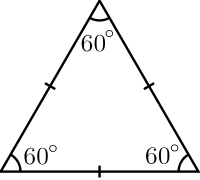
\includegraphics[scale=0.25]{images/200px-Triangle-Equilateral.png}~~~~~~
}
\subfigure[Isosceles Triangle]{
~~~~~~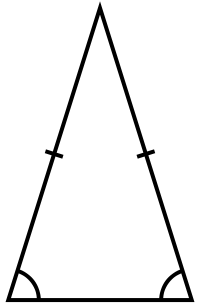
\includegraphics[scale=0.20]{images/200px-Triangle-Isosceles.png}~~~~~~
}
\subfigure[Scalene Triangle]{
~~~~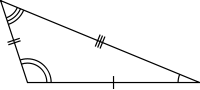
\includegraphics[scale=0.50]{images/200px-Triangle-Scalene.png}~~~~
}
\caption{Three types of triangles}
\label{figure:triangleTypes}
\end{figure}

\end{exer}

\begin{exer}
Body Mass Index (BMI) is a healthy statistic based on a person's mass and height.  For a healthy adult male
BMI is calculated as 
 $$\mathrm{BMI} = \frac{m}{h^2} \cdot 703.069579$$
where $m$ is the person's mass (in lbs) and $h$ is the person's height (in whole inches).  Write a program
that reads in a person's mass and height as input and outputs a characterization of the person's health with
respect to the categories in Table \ref{table:bmiCategories}.
\begin{table}[h]
\centering
\begin{tabular}{|l|l|}
\hline
Range & Category \\
\hline
\hline
$\mathrm{BMI} < 15$ & Very severely underweight \\
\hline
$15 \leq \mathrm{BMI} < 16$ & Severely underweight \\
\hline
$16 \leq \mathrm{BMI} < 18.5$ & Underweight \\
\hline
$18.5 \leq \mathrm{BMI} < 25$ & Normal \\
\hline
$25 \leq \mathrm{BMI} < 30$ & Overweight \\
\hline
$30 \leq \mathrm{BMI} < 35$ & Obese Class I \\
\hline
$35 \leq \mathrm{BMI} < 40$ & Obese Class II \\
\hline
$\mathrm{BMI} \geq 40$ & Obese Class III \\
\hline
\end{tabular}
\caption{BMI Categories}
\label{table:bmiCategories}
\end{table}
\end{exer}

\begin{exer}
Let $R_1$ and $R_2$ be rectangles in the plane defined as follows.  Let $(x_1, y_1)$ be
point corresponding to the lower-left corner of $R_1$ and let $(x_2, y_2)$ be the point of its
upper-right corner.  Let $(x_3, y_3)$ be point corresponding to the lower-left corner of $R_2$
and let $(x_4, y_4)$ be the point of its upper-right corner.

Write a program to determine the \emph{intersection} of these two rectangles.  In general,
the intersection of two rectangles is another rectangle.  However, if the two rectangles abut each
other, the intersection could be a horizontal or vertical line segment (or even a point).  It is also possible that the
intersection is \emph{empty}.  Your program will need to distinguish between these cases.

If the intersection of $R_1, R_2$ is a rectangle, $R_3$, your program should output two
points (the lower-left and upper-right corners of $R_3$) as well as the \emph{area} of $R_3$.
If the intersection is a line segment, your program should output the two \emph{end-points}
and whether it is a vertical or horizontal line segment.  Finally, if the intersection is empty your
program should output ``empty intersection''.  Your program should also be robust enough to
check that the input is valid (it should not accept empty or ``reversed'' rectangles).

Your program should read in $x_1, y_1, x_2, y_2, x_3, y_3, x_4, y_4$ from the user and
perform the computation above.  As an example, the values  $2, 1, 6, 7.5, 4, 5.5, 8.5, 8.25$
would correspond to the two rectangles in Figure \ref{fig:rectangleIntersection}.

\begin{figure}
\centering

\begin{tikzpicture}[scale=0.75]
  \draw[step=1.0cm,black!10!white,very thin] (-0.4,-0.4) grid (9,9); %
  \draw[->] (-0.6,0) -- (9.5,0) node[right] {$x$};%
  \draw[->] (0,-0.6) -- (0,9.5) node[above] {$y$};%

  \filldraw[fill=red,thick,fill opacity=.25] (2, 1) rectangle (6, 7.5);
  \filldraw[fill=green,fill opacity=.25] (4, 5.5) rectangle (8.5, 8.25);

  \fill (2, 1) circle (2pt);
  \fill (6, 7.5) circle (2pt);
  \fill (4, 5.5) circle (2pt);
  \fill (8.5, 8.25) circle (2pt);

  \node [] (A) at (2, 1) [below left] {$(2, 1)$};
  \node [] (B) at (6, 7.5) [above right] {$(6, 7.5)$};
  \node [] (C) at (4, 5.5) [below left] {$(4, 5.5)$};
  \node [] (D) at (8.5, 8.25) [above right] {$(8.5, 8.25)$};

\end{tikzpicture}

\caption{Intersection of Two Rectangles}
\label{fig:rectangleIntersection}
\end{figure}

The output for this instance should look something like the following.

\begin{minted}{text}
Intersecting rectangle: (4, 5.5), (6, 7.5)
Area: 4.00
\end{minted}
\end{exer}

\begin{exer}
Write an app to help people track their cell phone usage.  Cell 
phone plans for this particular company give you a certain number of minutes
every 30 days which must be used or they are lost (no rollover).  We want
to track the average number of minutes used per day and inform the user
if they are using too many minutes or can afford to use more.

Write a program that prompts the user to enter the following pieces of data:
\begin{itemize}
  \item Number of minutes in the plan per 30 day period, $m$
  \item The current day in the 30 day period, $d$
  \item The total number of minutes used so far $u$
\end{itemize}
The program should then compute whether the user is over, under, or 
right on the average daily usage under the plan.  It should also inform
them of how many minutes are left and how many, on average, they can
use per day for the rest of the month.  Of course, if they've run out of minutes, it
should inform them of that too.

For example, if the user enters $m = 250$, $d = 10$, and $u = 150$, your
program should print out something similar to the following.

\begin{minted}{text}
10 days used, 20 days remaining
Average daily use: 15 min/day

You are EXCEEDING your average daily use (8.33 min/day), 
continuing this high usage, you'll exceed your minute plan by
200 minutes.

To stay below your minute plan, use no more than 5 min/day.
\end{minted}

Of course, if the user is under their average daily use, a different
message should be presented.  You are allowed/encouraged to 
compute any other stats for the user that you feel would be useful.
\end{exer}

\begin{exer}
Write a program to  help a floor tile company determine how many
tiles they need to send to a work site to tile a floor in a room.  For 
simplicity, assume that all rooms are perfectly rectangular with no 
obstructions; we will also omit any additional measurements related 
to grouting.  

Further, we will assume that all tile is laid in a grid pattern centered 
at the center of the room.  That is, four tiles will meet at their corners 
at the center of the room with tiles laid out to the edge of the room.  
Thus, it may be the case that the final row and/or column at the edge 
may need to be cut.  Also note that if the cut is short enough, the 
remaining tile can be used on the other end of the room (same goes 
for the corners).

The program will take the following input:
\begin{itemize}
  \item $w$ - the width of the room
  \item $l$ - the length of the room
  \item $t$ - width/length of the tile (all tiles are perfectly square)
\end{itemize}

If we can use whole tiles to perfectly fit the room, then we do so.  
For example, on the input $(10, 10, 1)$, we could perfectly tile a 
$10 \times 10$ room with 100 $1 \times 1$ tiles.  If the tiles don't 
perfectly fit, then we have to consider the possibility of waste 
and/or reuse.  Consider the examples in Figure \ref{figure:floorTiling}.

\begin{figure}
\centering

\subfigure[Example 1] {
\begin{tikzpicture}[scale=.5]

\draw[step=1cm] (-4.8, -5) grid (4.8, 5);

\draw[very thick] (-4.8, -5) -- (4.8, -5) -- (4.8, 5) -- (-4.8, 5) -- (-4.8, -5);

\draw[decorate,decoration={brace,mirror}] (-4.8, -5.2) -- (-4, -5.2) node[midway,below] {0.9};
\draw[decorate,decoration={brace,mirror}] (4, -5.2) -- (4.8, -5.2) node[midway,below] {0.9};

\draw[decorate,decoration={brace,mirror}] (-5, -6.2) -- (5, -6.2) node[midway,below] {9.8};

\draw[decorate,decoration={brace,mirror}] (5.2, -5) -- (5.2, 5)  node [midway,right] {10.0};

\node (A) at (2,2) [rectangle,draw=black!50,fill=white] {Center of the room};
\draw[->] (A) -- (0,0);
\end{tikzpicture}
}
\subfigure[Example 2] {
\begin{tikzpicture}[scale=.5]

\draw[step=1cm] (-4.4, -5) grid (4.4, 5);

\draw[very thick] (-4.4, -5) -- (4.4, -5) -- (4.4, 5) -- (-4.4, 5) -- (-4.4, -5);

\draw[decorate,decoration={brace,mirror}] (-4.4, -5.2) -- (-4, -5.2) node[midway,below] {0.4};
\draw[decorate,decoration={brace,mirror}] (4, -5.2) -- (4.4, -5.2) node[midway,below] {0.4};

\draw[decorate,decoration={brace,mirror}] (-4.4, -6.2) -- (4.4, -6.2) node[midway,below] {8.8};

\draw[decorate,decoration={brace,mirror}] (4.6, -5) -- (4.6, 5)  node [midway,right] {10.0};

\node (A) at (2,2) [rectangle,draw=black!50,fill=white] {Center of the room};
\draw[->] (A) -- (0,0);
\end{tikzpicture}
}
\caption{Examples of Floor Tiling}
\label{figure:floorTiling}
\end{figure}


The first example is from the input $(9.8, 100, 1)$.  In this case, 
we lay the tiles from the center of the room (8 full tile lengths) but 
are left with $0.9$ on either side.  If we cut a tile to fit the left
side, we are left with only $.1$ tile which is too short for the right 
side.  Therefore, we are forced to waste the $0.1$ length and cut 
a full tile for the right side.  In all, 100 tiles are required.

The second example is from the input $(8.8, 100, 1)$.  In this case, 
we again lay tiles from the center of the room (8 full tile lengths) and 
are left with $0.4$ lengths on either side.  Here, we \emph{can}
reuse the cut tile: cut a tile on one side $0.4$ with $0.6$ remaining, 
and cut $0.4$ on the other side of the tile (with the center $0.2$ 
length of the tile being waste).  Thus, both sides can be tiled with 
a single tile, meaning only 90 full tiles are needed to tile this room.

You may further assume that tiles used on 
the length-side end of the room \emph{cannot} be used to tile the 
width-side of the room (and vice versa).  Your program will compute 
and output the number of tiles required.
\end{exer}




%CHAPTER: Loops
\chapter{Loops}
\label{chapter:loops}
\index{loops}
%!TEX root = ComputerScienceOne.tex

%%Chapter: Loops

Computers are really good at automation.  A key aspect of automation is 
the ability to repeat a process over and over on different pieces of data until some condition
is met.  For example, if we have a collection of numbers and we want to find their
sum we would \emph{iterate} over each number, adding it to a total, until we have
examined every number.  Another example may include sending an email message
to each student in a course.  To automate the process, we could iterate over each
student record and \emph{for each} student we would generate and send the email.

Automated repetition is where \emph{loops} come in handy.  Computers are perfectly suited 
for performing such repetitive tasks.  We can write a single block of code that performs
some action or processes a single piece of data, then we can write a loop around that
block of code to execute it a number of times.

Loops provide a much better alternative than repeating (cut-paste-cut-paste) the same
code over and over with different variables.  Indeed, we wouldn't even do this in real life.
Suppose that you took a 100 mile trip.  How would you describe it?  Likely,
you wouldn't say, ``I drove a mile, then I drove a mile, then I drove a mile, $\ldots$'' repeated
100 times.  Instead, you would simply state ``I drove 100 miles'' or maybe even, ``I drove
until I reached my destination.''  

Loops allow us to write concise, repeatable code that can be applied to each element in 
a collection or perform a task over and over again until some condition is met.  When 
writing a loop, there are three essential components:

\begin{itemize}
  \item An \emph{initialization} statement that specifies how the loop begins
  \item A \emph{continuation} (or \emph{termination}) condition that specifies whether the loop 
  	should continue to execute or terminate
  \item An \emph{iteration} statement that makes progress toward the termination condition
\end{itemize}

The initialization statement is executed before the loop begins and serves as a way
to set the loop up.  Typically, the initialization statement involves setting the initial value 
of some variable.

\begin{figure}
\centering
\begin{tikzpicture}[node distance=3cm,auto,scale=1.0,transform shape]
    % Place nodes
    
%    \tikzstyle{decision} = [diamond, draw, fill=blue!20, 
%    text width=4.5em, text badly centered, node distance=3cm, inner sep=0pt]
%\tikzstyle{block} = [rectangle, draw, fill=blue!20, 
%    text width=5em, text centered, rounded corners, minimum height=4em]
%\tikzstyle{line} = [draw, -latex']

    \node [block,text width=8em] (a) {Initialization: $i \leftarrow 1$};
    \node [decision,node distance=3.5cm,text width=6em,text centered, below of=a] (decide) {Continuation: $i \leq 10$?};
    \node [block,text width=8em, fill=green!20, below of=decide] (body) {loop body};
    \node [block,text width=8em, below of=body] (c) {Iteration: $i \leftarrow (i + 1)$};
    \node[block,node distance=3.5cm,text width=8em,below of=c] (d) {remaining program};
    
    %position dummy nodes
    %\node[right of=b] (null1) {};
    %\node[right of=decide] (null2) {};
    
    % Draw edges
    \path [line] (a) -- (decide);
    \path [line] (body) -- (c);
    %\path [line] (c) -- (d);
    \path [line] (decide) -- node {true} (body);
    \path [line] (c)   --++  (-3,0) node[below] {repeat} |- (decide);
    \path [line] (decide)   --++  (3,0) node [above] {false} |- (d);

% \path [line] (decide)   --++  (3,0) node [below] {true} |- (b);
%    \path [line] (decide) |- (null1) -- (null2) -| (b);
    %\path [line] (decide) |- node{true} (b);

%    \path [line] (decide) -- node {true}(a);
  %  \path [line] (decide) -- node {false}(b);
    %\path [line] (a) |- (c);
    %\path [line] (b) -- (c);
\end{tikzpicture}
\caption{A Typical Loop Flow Chart}
\label{figure:loopFlowChart}
\end{figure}

The continuation statement is a logical statement (that evaluates to \emph{true} or \emph{false})
that specifies if the loop should continue (if the value is \emph{true}) or should terminate
(if the value is \emph{false}).  Upon termination, code returns to a sequential control flow and
the program continues.  

The iteration statement is intended to update the state of a program to make progress
toward the termination condition.  If we didn't make such progress, the loop would continue
on forever as the termination condition would never be satisfied.  This is known as an \index{infinite loop} \emph{infinite loop} \index{infinite loop}, and results in a program that never terminates.

As a simple example, consider the following outline.

\begin{itemize}
  \item Initialize the value of a variable $i$ to 1
  \item While the value of $i$ is less than or equal to $10\ldots$ (continuation condition)
  \item Perform some action (this is sometimes referred to as the \emph{loop body}
  \item Iterate the variable $i$ by adding one to its value
\end{itemize}

The code outline above specifies that some action is to be performed once for
each value: $i=1, i=2, \ldots, i=10$, after which the loop terminates.  Overall, the
loop executes a total of 10 times.  Prior to each of the 10 executions, the value of $i$
is checked; as it is less than or equal to 10, the action is performed.  At the end of
each of the 10 iterations, the variable $i$ is incremented by 1 and the termination
condition is checked again, repeating the process.  There are several different types of loops that vary in syntax and style but they 
all have the same three basic components. 

\section{While Loops}
\index{while loop}
\index{loops!while loop}

A \emph{while loop} is a type of loop that places the three components in their 
logical order.  The initialization statement is written before the loop code.  
Typically the keyword \textsc{while} is used to specify the continuation/termination
condition.  Finally, the iteration statement is usually performed at the end of the loop
\emph{inside} the code block associated with the loop.  A small, counter-controlled 
while loop is presented in Algorithm \ref{algo:counterControlledWhileLoop} which 
illustrates the previous example of iterating a variable $i$ from 1 to 10.

\begin{algorithm}[H]
\caption{Counter-Controlled While Loop}
\label{algo:counterControlledWhileLoop}
$i \leftarrow 1$ \Comment{Initialization statement}
\While{$\left( i \leq 10 \right)$}{ 
  Perform some action \;
  $i \leftarrow (i + 1)$ \Comment{Iteration statement}
}
\end{algorithm}

Prior to the \textsc{while} statement, the variable $i$ is initialized to $1$.  This action
is only performed once and it is done so before the loop code.  Then, before the loop
code is executed, the continuation condition is checked.  Since $i = 1 \leq 10$, the 
condition evaluates to \emph{true} and the loop code block is executed.  The last
line of the code block is the iteration statement, where $i$ is incremented by 1 and
now has a value of $2$.  The code returns to the \emph{top} of the loop and again
evaluates the continuation condition (which is still true as $i = 2 \leq 10$).  

On the 10th iteration of the loop when $i = 10$, the loop will execute for the last
time.  At the end of the loop, $i$ is incremented to 11.  The loop \emph{still} returns
to the top and the continuation condition is \emph{still} checked one last time.  However,
since $i = 11 \not\leq 10$, the condition is now \emph{false} and the loop terminates.
Regular sequential control flow returns and the program continues executing whatever
code is specified after the loop.

\subsection{Example}
\label{subsection:whileLoopExample}

In the previous example we knew that we wanted the loop to execute ten
times.  Though you can use a while loop in counter-controlled situations, while loops are 
typically used in scenarios when you may not know how many iterations you want 
the loop to execute for.  Instead of a straightforward iteration, the loop itself may
update a variable in a less-than-predictable manner.  

As an example, consider the problem of \emph{normalizing} a number as is typically done in scientific notation.  Given a number $x$ (for simplicity, we'll consider $x \geq 1$),
we divide it by 10 until its value is in the interval $[1, 10)$, keeping track of how many times we've 
divided by 10.  For example, if we have the number $x = 32,145.234$, we would divide
by 10 four times, resulting in $3.2145234$ so that we could express it as
  $$3.2145234 \times 10^{4}$$
A simple realization of this process is presented in Algorithm 
\ref{algo:normalizingNumberWhileLoop}.  Rather than some fixed number of
iterations, the number of times the loop executes depends on how large $x$ is.  For the example
mentioned, it executes 4 times; for an input of $x = 10,000,000$ it would execute 7 times.
A while loop allows us to specify the repetition process without having to know up front
how many times it will execute.

\begin{algorithm}[H]
\caption{Normalizing a Number With a While Loop}
\label{algo:normalizingNumberWhileLoop}
\Input{A number $x$, $x \geq 0$}
\Output{$x$ normalized, $k$ its exponent}
$k \leftarrow 0$ \;
\While{$x > 10$}{
  $x \leftarrow (x / 10)$ \;
  $k \leftarrow (k + 1)$ \; 
}
output $x, k$ \;
\end{algorithm}

\section{For Loops}
\index{for loop}
\index{loops!for loop}

A \emph{for loop} is similar to a while loop but allows you to specify 
the three components on the same line.  In many cases, this results in a loop that
is more readable; if the code block in a while loop is long it may be difficult to see
the initialization, continuation, and iteration statements clearly.  For loops are 
typically used to iterate over elements stored in a collection such as an
array (see Chapter \ref{chapter:arrays}).  Usually the keyword \textsc{for} is used to identify all three components.  
A general example is given in Algorithm \ref{algo:generalForLoop}.

\begin{algorithm}[]
\caption{A General For Loop}
\label{algo:generalForLoop}
\For{$\left(\right. \langle initialization \rangle$; $\langle continuation \rangle$; $\langle iteration \rangle \left.\right)$}{
  Perform some action \;
}
\end{algorithm}

Note the additional syntax: in many programming languages, semicolons are used
at the end of executable statements.  Semicolons are also used to delimit each of
the three loop components in a for-loop (otherwise there may be some ambiguity as
to where each of the components begins and ends).  However, the semicolons are
typically only placed after the initialization statement and continuation condition and 
are \emph{omitted} after the iteration statement.  A more concrete example is given in 
Algorithm \ref{algo:counterControlledForLoop} which is equivalent
to the counter-controlled while loop we examined earlier.

\begin{algorithm}[h]
\caption{Counter-Controlled For Loop}
\label{algo:counterControlledForLoop}
\For{$\left(\right.$ $i \leftarrow 1$; $i \leq 10$; $i \leftarrow (i + 1)$ $\left.\right)$}{
  Perform some action \;
}
\end{algorithm}

Though all three components are written on the same line, the initialization statement
is only ever executed once; at the beginning of the loop.  The continuation condition is
checked prior to each and every execution of the loop.  Only if it evaluates to \emph{true}
does the loop body execute.  The iteration condition is performed \emph{at the end} of
each loop iteration.  

\subsection{Example}
\label{subsection:summationExample}

As a more concrete example, consider Algorithm \ref{algo:summationForLoop} in which 
we do the same iteration ($i$ will take on the values $1, 2, 3, \ldots, 10$), but in each 
iteration we add the value of $i$ \emph{for that iteration} to a running total, $sum$.

\begin{algorithm}[h]
\caption{Summation of Numbers in a For Loop}
\label{algo:summationForLoop}
$sum \leftarrow 0$ \;
\For{$\left(\right.$ $i \leftarrow 1$; $i \leq 10$; $i \leftarrow (i + 1)$ $\left.\right)$}{
  $sum \leftarrow (sum + i)$ \;
}
\end{algorithm}

Again, the initialization of $i = 1$ is only performed once.  On the first iteration of the loop, 
$i = 1$ and so $sum$ will be given the value $sum + i = 0 + 1 = 1$  At the end of the loop, 
$i$ will be incremented and will have a value of $2$.  The continuation condition is still satisfied, 
so once again the loop body executes and $sum$ will be given the value $sum + i = 1 + 2 = 3$.
On the 10th (last) iteration, $sum$ will have a value $1 + 2 + 3 + \cdots + 9 = 45$ and $i = 10$.
Thus $sum + i = 45 + 10 = 55$ after which $i$ will be incremented to 11.  The continuation condition
is \emph{still} checked, but since $11 \not\leq 10$, the loop body will not be executed and
the loop will terminate, resulting in a final $sum$ value of $55$.

\section{Do-While Loops}
\index{do-while loop}
\index{loops!do-while loop}

Yet another type of loop is the \emph{do-while} loop.  One major difference between this
type of loop and the others is that it is always executed \emph{at least once}.  The way that
this is achieved is that the continuation condition is checked \emph{at the end} of the loop
rather than prior to is execution.  The same counter-controlled example can be found in
Algorithm \ref{algo:counterControlledDoWhileLoop}.

\begin{algorithm}[h]
\caption{Counter-Controlled Do-While Loop}
\label{algo:counterControlledDoWhileLoop}
$i \leftarrow 1$ \;
\Do{$i \leq 10$}{
  Perform some action \;
  $i \leftarrow (i + 1)$ \;
}
\end{algorithm}

In contrast to the previous examples, the loop body is executed on the first iteration without
checking the continuation condition.  Only after the loop body, including the incrementing of 
the iteration variable $i$ is the continuation condition checked.  If \emph{true}, the loop repeats
at the beginning of the loop body.

\begin{figure}[!h]
%\begin{wrapfigure}[35]{R}{0.50\textwidth}
\centering
\begin{tikzpicture}[node distance=3cm,auto,scale=1.0,transform shape]
    % Place nodes
    
%    \tikzstyle{decision} = [diamond, draw, fill=blue!20, 
%    text width=4.5em, text badly centered, node distance=3cm, inner sep=0pt]
%\tikzstyle{block} = [rectangle, draw, fill=blue!20, 
%    text width=5em, text centered, rounded corners, minimum height=4em]
%\tikzstyle{line} = [draw, -latex']

    \node [block,text width=8em] (a) {Initialization: $i \leftarrow 1$};
    \node [block,text width=8em, fill=green!20, below of=a] (b) {loop body};
    \node [block,text width=8em, below of=b] (c) {Iteration: $i \leftarrow (i + 1)$};
    \node [decision,node distance=3.5cm,text width=6em,text centered, below of=c] (decide) {Continuation: $i \leq 10$?};
    \node[block,node distance=3.5cm,text width=8em,below of=decide] (d) {remaining program};
    
    %position dummy nodes
    %\node[right of=b] (null1) {};
    %\node[right of=decide] (null2) {};
    
    % Draw edges
    \path [line] (a) -- (b);
    \path [line] (b) -- (c);
    \path [line] (c) -- (decide);
    \path [line] (decide) -- node {false} (d);
    \path [line] (decide)   --++  (3,0) node [below] {true} |- (b);
%    \path [line] (decide) |- (null1) -- (null2) -| (b);
    %\path [line] (decide) |- node{true} (b);

%    \path [line] (decide) -- node {true}(a);
  %  \path [line] (decide) -- node {false}(b);
    %\path [line] (a) |- (c);
    %\path [line] (b) -- (c);
\end{tikzpicture}
\caption{A Do-While Loop Flow Chart.  The continuation condition is checked \emph{after} the loop body.}
\label{figure:doWhileLoopFlowChart}
%\end{wrapfigure}
\end{figure}

Do-while loops are typically used in scenarios in which the first iteration is used to ``setup'' 
the continuation condition (thus, it needs to be executed at least once).  A common example
is if the loop body performs an operation that may result in an error code (or flag) that is
either \emph{true} (an error occurred) or \emph{false} (no error occurred).  

\begin{algorithm}[h]
\caption{Flag-Controlled Do-While Loop}
\label{algo:flagControlledDoWhileLoop}
\Do{isError}{
  Read some data \;
  isError $\leftarrow$ result of reading \;
}
\end{algorithm}

From this perspective, a do-while loop can also be seen as a do-until loop: perform a task
\emph{until} some condition is no longer satisfied.  The subtle wording difference implies that
we'll perform the action before checking to see if it should be performed again.

\section{Foreach Loops}
\label{section:foreachLoops}
\index{foreach loop}
\index{loops!foreach loop}

Many languages support a special type of loop for iterating over individual elements in 
a collection (such as a set, list, or an array).  In general, such loops are referred to as \emph{foreach}
loops.  These types of loops are essentially \gls{syntactic sugar}: iterating over a collection
could be achieved with a for loop or a while loop, but foreach loops provide a more
convenient way to iterate over a collections.  We will revisit these loops
when we examine arrays in Chapter \ref{chapter:arrays}.  For now, we look at a simple example
in Algorithm \ref{algo:foreachLoop}.

\begin{algorithm}[h]
\caption{Example Foreach Loop}
\label{algo:foreachLoop}
\ForEach{element $a$ in the collection $A$}{
  process the element $a$ \;
}
\end{algorithm}

How the elements are stored in the collection and how they are iterated over is not our 
(primary) concern.  We simply want to apply the same block of code to each element, 
the foreach loop handles the details on how each element is iterated over.  The syntax
also provides a way to refer to each element (the $a$ variable in the algorithm).  On
each iteration of the loop, the foreach loop updates the reference $a$ to the \emph{next}
element in the array.  The loop terminates after it has iterated through each and every
one of the elements.  In this way, a foreach loop simplifies the syntax: we don't have to 
specify any of the three components ourselves.  As a more
concrete example, consider iterating over each student in a course roster.  For each
student, we wish to compute their grade and then email them the results.  The foreach
loop allows us to do this without worrying about the iteration details (see Algorithm 
\ref{algo:foreachGradeLoop}).

\begin{algorithm}[h]
\caption{Foreach Loop Computing Grades}
\label{algo:foreachGradeLoop}
\ForEach{(student $s$ in the class $C$)}{
  $g \leftarrow $ compute $a$'s grade \;
  send $a$ an email informing them of their grade $g$ \;
}
\end{algorithm}

\section{Other Issues}

\subsection{Nested Loops}
\index{nested loops}

Just as with conditional statements, we can nest loops within loops to perform
more complex processes.  Though you can do this with any type of loop, we 
present a simple example using for loops in Algorithm \ref{algo:nestedForLoops}.

\begin{algorithm}[h]
\caption{Nested For Loops}
\label{algo:nestedForLoops}
$n \leftarrow 10$ \;
$m \leftarrow 20$ \;
\For{($i \leftarrow 1$; $i \leq m$; $i \leftarrow (i + 1)$)}{
  \For{($j \leftarrow 1$; $j \leq n$; $j \leftarrow (j + 1)$)}{
    output $(i, j)$ \;
  }
}
\end{algorithm}

The outer for loop executes a total of 20 times while the inner for loop 
executes 10 times.  Since the inner for loop is \emph{nested} inside the 
outer loop, the entire inner loop executes all 10 iterations \emph{for each}
of the 20 iterations of the outer loop.  Thus, in total the inner most output
operation executes $10 \times 20 = 200$ times.  Specifically, it outputs 
$(1, 1), (1, 2), \ldots, (1, 10), (2, 1), (2, 2), \ldots, (2, 10), (3, 1), \ldots, (20, 10)$.  Nested loops are comment when iterating over elements 
in two-dimensional 
arrays such as tabular data or matrices.  Nested loops can also be used 
to process all \emph{pairs} in a collection of elements.

\subsection{Infinite Loops}
\label{subsection:infiniteLoops}
\index{infinite loop}
\index{loops!infinite loop}

Sometimes a simple mistake in the design of a loop can make it execute forever.  
For example, if we accidentally iterate a variable in the wrong direction or write the
\emph{opposite} termination/continuation condition.  Such a loop is referred to as 
an \emph{infinite loop}.  As an example, suppose we forgot the increment operation
from a previous example.

\begin{algorithm}[h]
\caption{Infinite Loop}
\label{algo:infiniteLoop}
$sum \leftarrow 0$ \;
$i \leftarrow 1$ \;
\While{$i \leq 10$}{
  $sum \leftarrow (sum + i)$ \;
}
\end{algorithm}

In Algorithm \ref{algo:infiniteLoop} we never make progress toward the terminating
condition!  Thus, the loop will execute forever, $i$ will continue to have the value 0
and since $0 \leq 10$, the loop body will continue to execute.  Care is needed in the
design of your loops to ensure that they make progress toward the termination condition.

Most of the time an infinite loop is not something you want and usually you must 
terminate your buggy program externally (sometimes referred to as ``killing'' it).  
However, infinite loops do have their uses.  A \emph{poll} loop is a loop that is
\emph{intended} to not terminate.  At a system level, for example, a computer
may \emph{poll} devices (such as input/output devices) one-by-one to see if
there is any active input/output request.  Instead of terminating, the poll loop
simply repeats itself, returning back to the first device.  As long as the computer
is in operation, we don't want this process to stop.  This can be viewed as an 
infinite loop as it doesn't have any termination condition.

\subsubsection{The Zune Bug}
\label{subsubsection:zuneBug}

Though proper testing and debugging should reduce the likelihood of such bugs,
there are several notable instances in which an infinite loop impacted real 
software.  One such instance was the Microsoft \emph{Zune} bug.  The Zune
was a portable music player, a competitor to the iPod.  At about midnight on 
the night of December 31st, 2008, Zunes everywhere failed to startup properly.
A firmware clock driver designed by a 3rd party company contained the following
code. 

\begin{listing}[!h]
\begin{minted}{c}
  while(days > 365) {
    if(IsLeapYear(year)) {
      if(days > 366) {
        days -= 366;
        year += 1;
     }
    } else {
      days -= 365;
      year += 1;
    }
  }
\end{minted}
  \caption{Zune Bug}
  \label{code:c:zuneBug}
\end{listing}

2008 was a leap year, so the check on line 2 evaluated to \emph{true}.
However, though December 31st, 2008 was the 366th day of the year (\mintinline{c}{days = 366})
the third line evaluated to \emph{false} and the loop was repeated without any of
the program state being updated.  The problem was ``fixed'' 24 hours later when 
it was the 367th day and line 3 worked.  The problem was that line 3 \emph{should} have been
\mintinline{c}{days >= 366)}.  

The failure was that this code was never tested on the 
``corner cases'' that it was designed for.  No one thought to test the driver to see
if it worked on the last day of a leap year.  The code worked the vast majority of the time, 
but this illustrates the need for rigorous testing.

\subsection{Common Errors}

When writing loops its important to use the proper syntax in the
language in which you are coding.  Many languages use semicolons
to terminate executable statements.  However, the \mintinline{c}{while}
statements are not executable: they are part of the control structure
of the language and do not have semicolons at the end.  A misplaced
semicolon could be a syntax error, or it could be syntactically correct
but lead to incorrect results.  A common error is to place a semicolon
at the end of a \mintinline{c}{while} statement as in 

\mintinline{c}{while(count <= 10); //WRONG!!!}

In this example, the \mintinline{c}{while} loop binds to an \emph{empty}
executable statement and results in an infinite loop!

Other common errors are the result of misidentifying either the
initialization statement or the continuation condition.  Starting a
counter at 1 instead of zero, or using a $\leq$ comparison instead
of a $<$ , etc.  These can lead to a loop being \emph{off-by-one} 
resulting in a logic error.

Other errors are the result of using improper variable types.
Recall that operations involving floating-point numbers can have 
round off and precision errors, $\frac{1}{3} + \frac{1}{3} + \frac{1}{3}$
may not be equal to one for example.  It is best to avoid using 
floating-point numbers or comparisons in the control of your loops.
Boolean and integer types are much less error prone.  

Finally, you must always ensure that your loops are making progress
\emph{toward} the termination condition.  A failure to properly 
increment a counter can lead to incorrect results or even an infinite
loop.

\subsection{Equivalency of Loops}

It might not seem obvious at first, but in fact, \emph{any} type of loop can be re-written 
as another type of loop and perform \emph{equivalent} operations.  That is, any while loop
can be rewritten as an equivalent for loop.  Any do-while loop can be rewritten as an 
equivalent while loop!  

So why do we have different types of loops?  The short answer is that we want our programming
languages to be flexible.  We could design a language in which every loop
\emph{had} to be a while loop for example, but there are some situations in which it would be 
more ``natural'' to write code with a for loop.  By providing several options, programmers have
the choice of which type of loop to write.  

In general, there are no ``rules'' as to which loop to apply to which situation.  There are general
trends, best practices, and situations where it is more common to use one loop rather than another,
but in the end it does come down to personal choice and style.  Some software projects or
organizations may have established guidelines or style guide that establishes such guidelines in the interest of consistency and uniformity.  

\section{Problem Solving With Loops}

Loops can be applied to any problem that requires repetition of some sort 
or to simplify
repeated code.  When designing loops, it is important to identify the three components by asking
the questions:
\begin{itemize}
  \item Where does the loop start?  What variables or other state may need to be initialized or setup
  	prior to the beginning of the loop?	
  \item What code needs to be repeated?  How can it be generalized to depend on loop control variables?
  	This helps you to identify and write the loop body.
  \item When should the loop end?  How many times do we want it to execute?  This helps you to 
  	identify the continuation and/or termination condition.
  \item How do we make progress toward the termination condition?  What variable(s) need to be incremented
  	and how?
\end{itemize}

\section{Examples}

\subsection{For vs While Loop}

Let's consider how to write a loop to compute the classic geometric series, 
  $$\frac{1}{1-x} = \sum_{k=0}^\infty x^k = 1 + x + x^2 + x^3 + \cdots$$
Obviously a computer cannot compute an infinite series as it is required to 
terminate in a finite number of steps.  Thus, we can approach this problem in
a number of different ways.  

One way we could approximate the series is to compute it out to a fixed
number of terms.  To do so, we could initialize a $sum$ variable to zero, then 
iteratively compute and add terms to the $sum$ until we have computed $n$ 
terms.  To keep track of the terms, we can define a counter variable, $k$ as in 
the summation.  

Following our strategy, we can identify the initialization: $k$ should start at $0$.
The iteration is also easy: $k$ should be incremented by 1 each time.  The 
continuation condition should continue the loop until we have computed $n$ terms.
However, since $k$ starts at 0, we would want to continue while $k < n$.  We
would not want to continue the iteration when $k = n$ as that would make $n + 1$
iterations (again since $k$ starts at 0).  Further, since we know the number of
iterations we want to execute, a for loop is arguably the most appropriate loop
for this problem.  Our solution is presented in Algorithm \ref{algo:geometricSeriesForLoop}.

\begin{algorithm}[h]
\caption{Computing the Geometric Series Using a For Loop}
\label{algo:geometricSeriesForLoop}
\Input{$x$, $n \geq 0$}
\Output{An approximated value of $\frac{1}{1-x}$ using a geometric series}
$sum \leftarrow 0$ \;
\For{($k = 0$; $k < n$; $k \leftarrow (k + 1)$)}{
  $sum \leftarrow (sum + x^k)$ \;
}
output $sum$ \;
\end{algorithm}

As an alternative, consider the following approach: instead of computing a 
predefined number of terms, what if we computed terms until the difference
between the value in the previous iteration and the value in the current 
iteration is negligible, say less than some small $\epsilon$ amount.  We could
stop our computation because any further iterations would only affect the 
summation less and less.  That is, the current value represents a ``good
enough'' approximation.  That way, if someone wanted an even better
approximation, they could specify a smaller $\epsilon$.

This approach will be more straightforward with a while loop since the 
continuation condition will be more along the lines of ``while the estimation
is not yet good enough, continue the summation.''  This approach will
also be easier if we keep track of both a \emph{current} and a \emph{previous}
value of the summation, then computing and checking the difference will
be easier.

\begin{algorithm}[h]
\caption{Computing the Geometric Series Using a While Loop}
\label{algo:geometricSeriesWhileLoop}
\Input{$x$, $\epsilon > 0$}
$sum_{prev} \leftarrow 0$ \;
$sum_{curr} \leftarrow 1$ \;
$k \leftarrow 1$ \;
\While{$|sum_{prev} - sum_{curr}| \geq \epsilon$}{
  $sum_{prev} \leftarrow sum_{curr}$ \;
  $sum_{curr} \leftarrow (sum_{curr} + x^k)$ \;
  $k \leftarrow (k + 1)$ \;
}
output $sum$ \;
\end{algorithm}

On lines 1--2 we initialize our values to ensure that the while loop will
execute at least once.  In the continuation condition, we use the absolute
value of the difference as the series can \emph{oscillate} between negative
and positive values.

\subsection{Primality Testing}

An integer $n > 1$ is called \emph{prime} if the only integers that 
divide it evently are 1 
and itself.  Otherwise it is called \emph{composite}.  For example, 30 is composite
as it is divisible by 2, 3, and 5 among others.  However, 31 is prime as it is only 
divisible by 1 and 31.

Consider the problem of determining whether or not a given integer $n$ is prime or 
composite, referred to as \emph{primality testing}.  A straightforward way of determining
this is to simply try dividing by every integer $2$ up to $\sqrt{n}$: if any of these integers
divides $n$, then $n$ is composite.  Otherwise, if none of them do, $n$ is prime.  
Observe that we only need to go up to $\sqrt{n}$ since any prime divisor greater
than that will correspond to \emph{some} prime divisor less than $\sqrt{n}$.

A simple for loop can be constructed to capture this idea. Our initialization clearly starts at $i = 2$, 
incrementing by 1 each time until $i$ has exceeded $\sqrt{n}$.  This solution
is presented in Algorithm \ref{algo:primalityTesting}.  Of course this is certainly
not the most efficient way to solve this problem, but we will not go into 
more advanced algorithms here.

\begin{algorithm}[h]
\caption{Determining if a Number is Prime or Composite}
\label{algo:primalityTesting}
\Input{$n > 1$}
\For{($i\leftarrow 2$; $i \leq \sqrt{n}$; $i \leftarrow (i + 1)$)}{
  \If{$i$ divides $n$}{
    output \emph{composite} \;
  }
}
output $prime$ \;
\end{algorithm}

Now consider this more general problem: given an integer $m > 1$, determine
\emph{how many} prime numbers $\leq m$ there are.  A key observation is that 
we've \emph{already solved} part of the problem: determining if a given number
is prime in the previous exercise.  To solve this more general problem, we could \emph{reuse}
or adapt our previous solution.  In particular, we could surround the previous
solution in an \emph{outer} loop and iterate over integers from 2 up to $m$.  
The inner loop would then determine if the integer is prime and instead of 
outputting a result, could increment a counter of the number of primes
it has found so far.
This solution is presented in Algorithm \ref{algo:primalityCounting}.

\begin{algorithm}[H]
\caption{Counting the number of primes.}
\label{algo:primalityCounting}
\Input{$m > 1$}
$numberOfPrimes \leftarrow 0$ \;
\For{($j=2$; $j\leq m$; $j \leftarrow (j + 1)$)}{
  $isPrime \leftarrow true$ \;
  \For{($i\leftarrow 2$; $i \leq \sqrt{j}$; $i \leftarrow (i + 1)$)}{
    \If{($i$ divides $j$)}{
      $isPrime \leftarrow false$ \;
    }
  }
  \If{($isPrime$)}{
    $numberOfPrimes \leftarrow (numberOfPrimes + 1)$ \;
  }
}
output $numberOfPrimes$ \;
\end{algorithm}

\subsection{Paying the Piper}
\label{subsection:loanAmortization}

Banks issue loans to customers as one lump sum called a \emph{principle} $P$ that
the borrower must pay back over a number of \emph{terms}.  Usually payments
are made on a monthly basis.  Further, banks charge an amount of \emph{interest} on a
loan measured as an Annual Percentage Rate (APR).  Given these conditions, 
the borrower makes monthly payments determined by the following formula.
$$ {monthlyPayment} = \frac{iP}{1 - (1 + i)^{-n}} $$
Where $i = \frac{apr}{12}$ is the monthly interest rate, and $n$ is the number of terms
(in months).

For simplicity, suppose we borrow $P = \$1,000$ at 5\% interest ($apr = 0.05$) to 
be paid back over a term of 2 years ($n = 24$).  Our monthly payment would 
(rounded) be 
  $$ {monthlyPayment} = \frac{\frac{.05}{12}\cdot 1000}{1 - (1 + \frac{.05}{12})^{-24}} = \$43.87$$
When the borrower makes the first month's payment, some of it goes to interest, 
some of it goes to paying down the balance.  Specifically, one month's interest on \$1,000 is
  $$\$1,000 \cdot \frac{0.05}{12} = \$4.17$$
and so $\$43.87 - \$4.17 = \$39.70$ goes to the balance, making the new balance
\$960.30.  The next month, this new balance is used to compute the new interest payment, 
  $$\$960.30 \cdot \frac{0.05}{12} = \$4.00$$
And so on until the balance is fully paid.  This process is known as \emph{loan amortization}.

Let's write a program that will calculate a loan amortization schedule given the 
inputs as described above.  To start, we'll need to compute the monthly payment
using the formula above and for that we'll need a monthly interest rate.  The
balance will be updated month-to-month, so we'll use another variable to represent the balance.  Finally, we'll want to track the current month in the loan 
schedule process.  

Once we have these variables setup, we can start a loop that will repeat once for
each month in the loan schedule.  We could do this using either type of loop, but
for this exercise, let's use a while loop.  Using our $month$ variable, we'll start by
initializing it to 1 and run the loop through the last month, $n$.  

On each iteration we compute that month's interest and principle payments as above, 
update the balance, and also be sure to update our $month$ counter variable to
ensure we're making progress toward the termination condition.  On each 
iteration we'll also output each of these variables to the user.  The full 
program can be found in Algorithm \ref{algo:loanAmortization}.

If we were to actually implement this we'd need to be more careful.  This outlines
the basic process, but keep in mind that US dollars are only accurate to cents.
A monthly payment can't be \$43.871 cents.  We'll need to take care to round
properly.  This introduces another issue: by rounding the final month's payment
may not match the expected monthly payment (we may over or under pay in the 
final month).  An actual implementation may need to handle the final month's 
payment separately with different logic and operations than are outside 
the loop.

\begin{algorithm}[H]
\Input{A principle, $P$, a number of terms, $n$, an APR, $apr$}
\Output{A loan amortization schedule}
$balance \leftarrow P$ \Comment{The initial balance is the principle}
$i \leftarrow \frac{apr}{12}$ \Comment{monthly interest rate}
$monthlyPayment \leftarrow \frac{iP}{1 - (1 + i)^{-n}} $ \;
$month \leftarrow 1$ \Comment{A month counter}
\While{($month \leq n$)}{
  $monthInterest \leftarrow i \cdot balance$ \;
  $monthPrinciple \leftarrow monthlyPayment - monthInterest$ \;
  $balance \leftarrow balance - monthPrinciple$ \;
  $month = (month + 1)$ \;
  output $month, monthInterest, monthPrinciple, balance$ \;
}
\caption{Computing a loan amortization schedule}
\label{algo:loanAmortization}
\end{algorithm}




%!TEX root = ComputerScienceOne.tex

%Loops - exercises

\section{Exercises}

\begin{exer}
Write a for-loop and a while-loop that accomplishes each of the following.
\begin{enumerate}
  \item[(a)] Prints all integers 1 thru 100 on the same line delimited by a single space
  \item[(b)] Prints all even integers 0 up to $n$ in reverse order
  \item[(c)] A list of integers divisible by 3 between $a$ and $b$ where $a, b$ are parameters or inputs
  \item[(d)] Prints all positive powers of two up to $2^{30}$ : $1, 2, 4, \ldots, 1073741824$ one value per line (try computing up to $2^{31}$ and $2^{32}$ and discern reasons for why it may fail)
  \item[(e)] Prints all even integers 2 thru 200 on 10 different lines (10 numbers on each line) \emph{in reverse order}
  \item[(f)] Prints the following pattern of numbers (hint: use two nested loops; the result can be computed using some value of $i + 10j$)
\end{enumerate}

\begin{minted}{text}
 11  21  31  41  51  61  71  81  91 101
 12  22  32  42  52  62  72  82  92 102
 13  23  33  43  53  63  73  83  93 103
 14  24  34  44  54  64  74  84  94 104
 15  25  35  45  55  65  75  85  95 105
 16  26  36  46  56  66  76  86  96 106
 17  27  37  47  57  67  77  87  97 107
 18  28  38  48  58  68  78  88  98 108
 19  29  39  49  59  69  79  89  99 109
 20  30  40  50  60  70  80  90 100 110
   \end{minted}
\end{exer}

\begin{exer}
Civil engineers have come up with two different models on how a city's 
population will grow over the next several years.  The first projection assumes
a 10\% annual growth rate while the second projection assumes a linear growth
rate of 50,000 additional citizens per year.  Write a program to project the
population growth under both models.  Take, as input, the initial population of
the city along with a number of years to project the population.

In addition, compute how many years it would take to \emph{double} the population
under each model.
\end{exer}

\begin{exer}
Write a loan program similar to the amortization schedule program we developed in 
Section \ref{subsection:loanAmortization}.  However, give the user an option to 
specify an \emph{extra} monthly payment amount in order to pay off the loan
early.  Calculate how much quicker the loan gets paid off and how much they
save in interest.  
\end{exer}

%\begin{exer}
%Write a Program to create a table containing a customized loan amortization table. Your program will
%prompt the user to enter the amount borrowed (the $\emph{principal}$), the annual interest rate(format: $\texttt{5.05}$ is
%5.5$\%$), and the number of monthly payments ($\emph{n}$). To calculate the monthly payment, use the following formula:
%$$ {payment} = \frac{iP}{1 - (1 + i)^{-n}} $$
%where
%\begin{itemize}
%  \item \emph{P} is the initial principal amount
%  \item \emph{i} is the monthly interest rate ($\frac{1}{12}$ of the APR)
%  \item \emph{n} is the total number of payments (payment periods)
%\end{itemize}
%Note that this payment must be rounded to the nearest cent. After the payment has been rounded to the nearest cent,
%the program will create a table that looks like the following.
%\begin{minted}{text}
%Principal: $1000.00
%Annual Interest Rate: 9.00 %
%Term: 6 months
%Monthly Payment: $171.07
%Payment     Interest       Principal        Balance
%1           $   7.50        $ 163.57       $ 836.43
%2           $   6.27        $ 164.80       $ 671.63
%3           $   5.04        $ 166.03       $ 505.60
%4           $   3.79        $ 167.28       $ 338.32
%5           $   2.54        $ 168.53       $ 169.79
%6           $   1.27        $ 169.79       $   0.00
%Final Payment: $171.06
%\end{minted}
%
%Each month, part of the payment is applied to the interest and the rest is applied to the principal
%Because the payment and each month's interest rate are rounded, the final payment will be a bit different
%and must be calculated as the sum of the final interest payment and the final principal balance.
%\end{exer}

\begin{exer}
The rate of decay of a radioactive
isotope is given in terms of its half-life $H$, the time lapse required
for the isotope to decay to one-half of its original mass. For example,
the isotope Strontium-90 ($^{90}Sr$) has a half-life of 28.9 years.  If
we start with 10kg of Strontium-90 then 28.9 years later you 
would expect to have only 5kg of Strontium-90 (and 5kg
of Yttrium-90 and Zirconium-90, isotopes which Strontium-90 decays
into).

Write a program that takes the following input:
\begin{itemize}
  \item Atomic Number (integer)
  \item Element Name
  \item Element Symbol
  \item $H$ (half-life of the element)
  \item $m$, an initial mass in grams
\end{itemize}

Your program will then produce a table detailing the amount of the element
that remains after each year until less than 50\% of the original amount remains.
This amount can be computed using the following formula:
  $$r = m \times \left(\frac{1}{2}\right)^{(y/H)}$$
$y$ is the number of years
elapsed, and $H$ is the half-life of the isotope in years.

For example, using your program on Strontium-90 (symbol: Sr, atomic number: 38)
with a half-life of 28.9 years and an initial amount of 10 grams would produce a table something like:
\begin{minted}{text}
 Strontium-90 (38-Sr)
Elapsed Years    Amount
-------------------------
-                10g
1                9.76g
2                9.53g
3                9.30g
...
28               5.11g
29               4.99g
\end{minted}
\end{exer}

\begin{exer}
In this exercise, you will develop a program that assists people in saving for a retirement
using a tax-deferred 401k program.  

Your application will allow a user to enter the following inputs:
\begin{itemize}
  \item An initial starting balance
  \item A monthly contribution amount (we'll assume its the same over the life of the savings plan)
  \item An (average) annual rate of return
  \item An (average) annual rate of inflation
\end{itemize}

In addition, your program will allow a user to choose between two different scenarios:
\begin{itemize}
  \item The first will allow the user to input a number of \emph{years} left until retirement.  
  	It will then compute a monthly savings table which will be a projection out to that many years.
  \item The second will take a \emph{target} dollar amount and compute a monthly savings
  	table until the account balance has reached this target dollar amount.
\end{itemize}

The monthly interest rate should be inflation-adjusted.  The inflation-adjusted 
rate of return can be computed with the following formula.
  $$\frac{1 + \textrm{rate of return}}{1+\textrm{inflation rate}} - 1$$
To get the monthly rate, simply divide by 12.  Each month, interest is applied to the balance at this 
rate along with the monthly contribution amount.

An example: if we start with \$10,000 and contribute \$500 monthly with a return rate of 9\% and
an inflation rate of 1.2\%, the first few lines of our table would something like the following.

\begin{minted}{text}
Payment     Interest Earned  Contribution   Balance
1           $   64.23        $ 500.00       $ 10564.23
2           $   67.85        $ 500.00       $ 11132.08
3           $   71.50        $ 500.00       $ 11703.58
4           $   75.17        $ 500.00       $ 12278.75
...
\end{minted}

\end{exer}

%applied math type problems

\begin{exer}
Write a program that computes various statistics on a collection of numbers that can
be read in from the command line, as command line arguments, or via other means.
In particular, given $n$ numbers, 
  $$x_1, x_2, \ldots, x_n$$
your program should compute the following statistics:
\begin{itemize}
  \item The minimum number
  \item The maximum number
  \item The mean,
   $$\mu = \frac{1}{n} \sum_{i=1}^n x_i$$
  \item The variance,
   $$\sigma^2 = \frac{1}{n} \sum_{i=1}^n (x_i - \mu)^2$$
  \item And the standard deviation,
   $$\sigma = \sqrt{\frac{1}{n} \sum_{i=1}^n (x_i - \mu)^2}$$
\end{itemize}
where $n$ is the number of numbers that was provided.  For example, with the numbers, 
  $$3.14, 2.71, 42, 3, 13$$
your output should look something like:

\begin{minted}{text}
Minimum:      2.71
Maximum:     42.00
Mean:        12.77
Variance:   228.77
Standard
Deviation:   15.13
\end{minted}
\end{exer}

\begin{exer}
The ancient Greek mathematician Euclid developed a method for finding
the greatest common divisor of two positive integers, $a$ and $b$. His method is
as follows:
\begin{enumerate}
  \item If the remainder of $a/b$ is 0 then $b$ is the greatest
      common divisor.
  \item If it is not 0, then find the remainder $r$ of $a/b$ and
      assign $b$ to $a$ and the remainder $r$ to $b$.
  \item Return to step (1) and repeat the process.
\end{enumerate}
Write a program that uses a function to perform this procedure. Display
the two integers and the greatest common divisor.
\end{exer}

%numerical analysis type math

\begin{exer}
Write a program to estimate the value of $e \approx 2.718281\ldots$ using the series: 
  $$e = \sum_{k=0}^{\infty} \frac{1}{k!}$$
Obviously, you will need to restrict the summation to a finite number of $n$ terms.
\end{exer}

\begin{exer}
The value of ${\pi}$ can be expressed by the following infinite series:
 $$ {\pi} = 4  \cdot \left( 1 - \frac{1}{3} + \frac{1}{5} - \frac{1}{7} + \frac{1}{9} - \frac{1}{11} + \frac{1}{13} - \cdots \right)$$
An approximation can be made by taking the first $n$ terms of the series.  For $n = 4$, the approximation is
 $$\pi \approx 4 \cdot \left( 1 - \frac{1}{3} + \frac{1}{5} - \frac{1}{7} \right) = 2.8952$$
Write a program that takes $n$ as input and outputs an approximation of $\pi$ according to the
series above.
\end{exer}

\begin{exer}
The sine function can be approximated using the following Taylor series.
  $$\sin{(x)} = \sum_{i=0}^{\infty} \frac{(-1)^i}{(2i+1)!} x^{2i+1} = x - \frac{x^3}{3!} + \frac{x^5}{5!} - \cdots$$
Write a function that takes $x$ and $n$ as inputs and approximates $\sin{x}$ by computing the first $n$
terms in the series above.
\end{exer}

\begin{exer}
One way to compute $\pi$ is to use Machin's formula:
  $$\frac{\pi}{4} = 4 \arctan{\frac{1}{5}} - \arctan{\frac{1}{239}}$$
To compute the $\arctan$ function, you could use the following series:
  $$\arctan{x} = \frac{x}{1} - \frac{x^3}{3} + \frac{x^5}{5} - \frac{x^7}{7} + \cdots = \sum_{i=0}^{\infty} \frac{(-1)^i}{2k+1} x^{2i + 1}$$
Write a program to estimate $\pi$ using these formulas but allowing
the user to specify how many terms to use in the series to compute it.
Compare the estimate with the built-in definition of $\pi$ in your language.  
\end{exer}

\begin{exer}
The \emph{arithmetic-geometric} mean of two numbers $x, y$, denoted $M(x, y)$ 
(or $\mathrm{agm}(x, y)$) can be computed iteratively as follows.  Initially, 
$a_1 = \frac{1}{2}(x + y)$ and $g_1 = \sqrt{xy}$ (i.e. the normal arithmetic and 
geometric means).  Then, compute
  $$\begin{array}{rcl}
    a_{n+1} & = & \frac{1}{2}(a_n+g_n) \\
    g_{n+1} & = & \sqrt{a_n g_n}
    \end{array}$$
The two sequences will converge to the same number which is the arithmetic-geometric 
mean of $x, y$.  Obviously we cannot compute an infinite sequence, so we compute until
$|a_n - g_n| < \epsilon$ for some small number $\epsilon$.
\end{exer}

\begin{exer}
The integral of a function is a measure of the area under its curve.  One numerical method for 
computing the integral of a function $f(x)$ on an interval $[a, b]$ is the \emph{rectangle} rule.
Specifically, an interval $[a, b]$ is split up into $n$ equal subintervals of size
$h = \frac{b-a}{n}$.  Then the integral is approximated by computing:
  $$\int_{a}^{b} f(x) dx \approx \sum_{i=0}^{n-1} f(a + ih) \cdot h$$
Write a program to approximate an integral using the rectangle method.  For this particular exercise you 
will integrate the function
  $$f(x) = \frac{\sin{x}}{x}$$
For reference, the function is depicted in Figure \ref{fig:sinxx}.  Write a program that will
read the end points $a, b$ and the number of subintervals $n$ and computes the integral 
of $f$ using the rectangle method.  It should then output the approximation.

\begin{figure}[h]
\centering
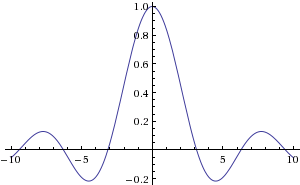
\includegraphics[scale=0.65]{images/sinxx}
\caption{Plot of $f(x) = \frac{\sin{x}}{x}$}
\label{fig:sinxx}
\end{figure}
\end{exer}

\begin{exer}
Another way to compute an integral is to a technique called \emph{Monte Carlo Integration}, 
a randomized numerical integration method.

Given the interval $[a, b]$, we enclose the function in a region of interest with a rectangle of a known
area $A_r$.  We then randomly select $n$ points within the rectangle and count the number of random
points that are within the function's curve.  If $m$ of the $n$ points are within the curve, we can estimate
the integral to be
 $$\int_a^b \! f(x) \, \mathrm{d} x \approx \frac{m}{n}A_r$$

Consider again the function $f(x) = \frac{\sin(x)}{x}$.  Note that the global maximum and 
minimum of this function are 1 and $\approx -0.2172$ respectively.
Therefore, we can also restrict the rectangle along the $y$-axis from $-.25$ to $1$.  That is, the lower
left of the rectangle will be $(a, -.25)$ and the upper right will be $(b, 1)$ for a known area of
 $$A_r = |a - b| \times 1.25$$
Figure \ref{fig:sinxxRect} illustrates the rectangle for the interval $[-5, 5]$.

\begin{figure}[h]
\centering
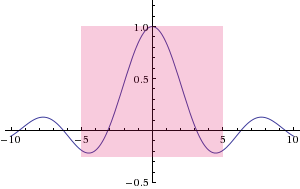
\includegraphics[scale=.75]{images/sinxxRect.png}
\caption{A rectangle for the interval $[-5, 5]$.}
\label{fig:sinxxRect}
\end{figure}

Write a program that will takes as input interval values $a, b$, and an integer $n$ and 
perform a Monte Carlo estimate of the integral of the function above.  Realize that this 
is just an approximation and it is randomized so your answers may not match exactly
and may be different on various executions of your program.  Take care that you handle 
points within the curve but under the $x$-axis correctly.
\end{exer}


\begin{exer}
Consider a ball trapped in a 2-D box.  Suppose that it has an initial position $(x, y)$ within the box
(the box's dimensions are specified by its lower left $(x_\ell, y_\ell)$ and an upper right $(x_r, y_r)$ points)
along with an initial angle of travel $\theta$ in the range $[0, 2\pi)$.  As the ball travels in this direction it
will eventually collide with one of the sides of the box and bounce off.  For this model, we will assume no loss of velocity
(it keeps going) and its angle of reflection is perfect.  

Write a program that takes as input, $x, y, \theta, x_\ell, y_\ell, x_r, y_r$, and an integer $n$
and computes the first $n-1$ Euclidean points on the box's perimeter that the ball bounces off of in its
travel (include the initial point in your printout for a total of $n$ points).  You may assume that the input will always be ``good'' (the ball will always begin somewhere inside the box
and the lower left and upper right points will not be reversed).

As an example, consider the inputs: 
$$x = 1, y=1, \theta = .392699, x_\ell = 0, y_\ell = 0, x_r = 4, y_r = 3,  n = 20$$
Starting at $(1, 1)$, the ball travels up and to the right bouncing off the right wall.  Figure 
\ref{fig:bouncyBall} illustrates this and the subsequent bounces back and forth.

\begin{figure}[h]
\centering
%\documentclass{article}
%\usepackage{tikz}
%\usetikzlibrary{arrows.meta}
%\begin{document}

\begin{tikzpicture}[scale=2.0]
  \draw[step=1.0cm,black!40!white,very thin] (-0.2,-0.2) grid (4.2,3.2); %
  \draw[thick,->] (0, -0.2) -- (0, 3.2) node[above] {$y$};%
  \draw[thick,->] (-0.2, 0) -- (4.2, 0) node[right] {$x$};%

  \filldraw[fill=green!70!white,fill opacity=.25] (0, 0) rectangle (4,3);

  \draw[fill] (1, 1) circle (1pt) node[below] {$(1, 1)$};
  \draw[fill] (4.000000, 2.242641) circle (1pt);
  \draw[->,shorten >=3pt,thick] (1.000000,1.000000) -- (4.000000,2.242641);
  \draw[fill] (2.171573, 3.000000) circle (1pt);
  \draw[->,shorten >=3pt,thick] (4.000000,2.242641) -- (2.171573,3.000000);
  \draw[fill] (0.000000, 2.100505) circle (1pt);
  \draw[->,shorten >=3pt,thick] (2.171573,3.000000) -- (0.000000,2.100505);
  \draw[fill] (4.000000, 0.443651) circle (1pt);
  \draw[->,shorten >=3pt,thick] (0.000000,2.100505) -- (4.000000,0.443651);
  \draw[fill] (2.928932, 0.000000) circle (1pt);
  \draw[->,shorten >=3pt,thick] (4.000000,0.443651) -- (2.928932,0.000000);
  \draw[fill] (0.000000, 1.213203) circle (1pt);
  \draw[->,shorten >=3pt,thick] (2.928932,0.000000) -- (0.000000,1.213203);
  \draw[fill] (4.000000, 2.870058) circle (1pt);
  \draw[->,shorten >=3pt,thick] (0.000000,1.213203) -- (4.000000,2.870058);
  \draw[fill] (3.686291, 3.000000) circle (1pt);
  \draw[->,shorten >=3pt,thick] (4.000000,2.870058) -- (3.686291,3.000000);
  \draw[fill] (0.000000, 1.473088) circle (1pt);
  \draw[->,shorten >=3pt,thick] (3.686291,3.000000) -- (0.000000,1.473088);
  \draw[fill] (3.556349, 0.000000) circle (1pt);
  \draw[->,shorten >=3pt,thick] (0.000000,1.473088) -- (3.556349,0.000000);
  \draw[fill] (4.000000, 0.183766) circle (1pt);
  \draw[->,shorten >=3pt,thick] (3.556349,0.000000) -- (4.000000,0.183766);
  \draw[fill] (0.000000, 1.840620) circle (1pt);
  \draw[->,shorten >=3pt,thick] (4.000000,0.183766) -- (0.000000,1.840620);
  \draw[fill] (2.798990, 3.000000) circle (1pt);
  \draw[->,shorten >=3pt,thick] (0.000000,1.840620) -- (2.798990,3.000000);
  \draw[fill] (4.000000, 2.502525) circle (1pt);
  \draw[->,shorten >=3pt,thick] (2.798990,3.000000) -- (4.000000,2.502525);
  \draw[fill] (0.000000, 0.845671) circle (1pt);
  \draw[->,shorten >=3pt,thick] (4.000000,2.502525) -- (0.000000,0.845671);
  \draw[fill] (2.041631, 0.000000) circle (1pt);
  \draw[->,shorten >=3pt,thick] (0.000000,0.845671) -- (2.041631,0.000000);
  \draw[fill] (4.000000, 0.811183) circle (1pt);
  \draw[->,shorten >=3pt,thick] (2.041631,0.000000) -- (4.000000,0.811183);
  \draw[fill] (0.000000, 2.468037) circle (1pt);
  \draw[->,shorten >=3pt,thick] (4.000000,0.811183) -- (0.000000,2.468037);
  \draw[fill] (1.284271, 3.000000) circle (1pt);
  \draw[->,shorten >=3pt,thick] (0.000000,2.468037) -- (1.284271,3.000000);

  \draw[fill] (1.284, 3) circle (1pt) node[above] {$(1.284, 3)$};  

\end{tikzpicture}

%\end{document}


\caption{Follow the bouncing ball}
\label{fig:bouncyBall}
\end{figure}

Your output should simply be the points and should look something like the following.

\begin{minted}{text}
(1.000000, 1.000000)
(4.000000, 2.242640)
(2.171572, 3.000000)
(0.000000, 2.100506)
(4.000000, 0.443652)
(2.928929, 0.000000)
(0.000000, 1.213202)
(4.000000, 2.870056)
(3.686287, 3.000000)
(0.000000, 1.473090)
(3.556355, 0.000000)
(4.000000, 0.183764)
(0.000000, 1.840617)
(2.798998, 3.000000)
(4.000000, 2.502529)
(0.000000, 0.845675)
(2.041640, 0.000000)
(4.000000, 0.811179)
(0.000000, 2.468033)
(1.284282, 3.000000)
\end{minted}

\end{exer}

\begin{exer}
An integer $n \geq 2$ is \emph{prime} if its only divisors are $1$ and itself, $n$.  For example, $2, 3, 5, 7, 11, \ldots$
are primes.  Write a program that outputs all prime numbers $2$ up to $m$ where $m$ is read as input.
\end{exer}

\begin{exer}
An integer $n \geq 2$ is \emph{prime} if the only integers that evenly divide it are $1$ and $n$ itself, 
otherwise it is \emph{composite}.  The \emph{prime factorization} of an integer is a list of its prime divisors 
along with their multiplicities.  For example, the prime decomposition of $188,760$ is:
  $$188,760 = 2 \cdot 2 \cdot 2 \cdot 3 \cdot 5 \cdot 11 \cdot 11 \cdot 13$$
Write a program that takes an integer $n$ as input and outputs the prime factorization of $n$.
If $n$ is invalid, an appropriate error message should be displayed instead.  Your output should look 
something like the following.
\begin{minted}{text}
1001 = 7 * 11 * 13
\end{minted}
\end{exer}

\begin{exer} 
One way of estimating $\pi$ is to randomly sample points within a $2 \times 2$ square centered
at the origin.  If the distance between the randomly chosen point $(x, y)$ and the origin is less than or
equal to 1, then the point lies inside the unit circle centered at the origin and we count it.  If the 
point lies outside the circle then we can ignore it.  
\begin{figure}[h]
\centering
%\documentclass{article}
%\usepackage{tikz}
%\begin{document}

\begin{tikzpicture}[scale=2.0]
  \draw[step=1.0cm,black!40!white,very thin] (-2.2,-2.2) grid (2.2,2.2); %
  \draw[<->] (0, -2.3) -- (0, 2.3) node[right] {$y$};%
  \draw[<->] (-2.3, 0) -- (2.3, 0) node[above] {$x$};%

  \filldraw[fill=yellow!70!white,thick,fill opacity=.25] (-1, -1) rectangle (1,1);
  \filldraw[fill=red,thick,fill opacity=.5] (0, 0) circle (1);

  \fill(-0.179025, 0.170052) circle(.35pt);
  \fill(-0.230483, -0.884416) circle(.35pt);
  \fill(0.440984, 0.444861) circle(.35pt);
  \fill(-0.086282, 0.089922) circle(.35pt);
  \fill(0.749824, -0.287103) circle(.35pt);
  \fill(0.782099, 0.656653) circle(.35pt);
  \fill(0.084703, 0.016307) circle(.35pt);
  \fill(-0.544334, -0.422176) circle(.35pt);
  \fill(-0.575099, -0.820715) circle(.35pt);
  \fill(-0.927591, 0.952768) circle(.35pt);
  \fill(-0.393389, -0.605339) circle(.35pt);
  \fill(-0.581804, 0.620439) circle(.35pt);
  \fill(-0.085225, 0.438428) circle(.35pt);
  \fill(0.676509, 0.337266) circle(.35pt);
  \fill(0.866596, 0.505712) circle(.35pt);
  \fill(-0.952575, -0.312428) circle(.35pt);
  \fill(-0.324235, -0.183058) circle(.35pt);
  \fill(-0.196845, -0.883251) circle(.35pt);
  \fill(-0.738196, 0.716873) circle(.35pt);
  \fill(0.206670, -0.988372) circle(.35pt);
  \fill(-0.570230, -0.011231) circle(.35pt);
  \fill(0.668280, 0.514473) circle(.35pt);
  \fill(-0.994924, -0.876053) circle(.35pt);
  \fill(-0.907703, -0.570023) circle(.35pt);
  \fill(-0.696768, -0.835294) circle(.35pt);
  \fill(-0.617255, -0.090158) circle(.35pt);
  \fill(-0.440633, -0.199060) circle(.35pt);
  \fill(-0.469719, 0.474141) circle(.35pt);
  \fill(-0.760632, -0.793210) circle(.35pt);
  \fill(-0.188592, -0.894036) circle(.35pt);
  \fill(0.712502, -0.141167) circle(.35pt);
  \fill(-0.206464, -0.611733) circle(.35pt);
  \fill(0.675775, 0.596692) circle(.35pt);
  \fill(-0.494985, 0.937579) circle(.35pt);
  \fill(0.313565, 0.711686) circle(.35pt);
  \fill(0.949207, 0.743335) circle(.35pt);
  \fill(-0.299545, 0.617487) circle(.35pt);
  \fill(0.257808, -0.294469) circle(.35pt);
  \fill(0.741434, 0.350105) circle(.35pt);
  \fill(0.135507, -0.955335) circle(.35pt);
  \fill(0.514811, 0.518252) circle(.35pt);
  \fill(-0.045492, -0.925822) circle(.35pt);
  \fill(-0.680808, 0.484789) circle(.35pt);
  \fill(0.548319, -0.441440) circle(.35pt);
  \fill(0.691579, -0.640273) circle(.35pt);
  \fill(-0.335475, 0.404081) circle(.35pt);
  \fill(0.218559, 0.458061) circle(.35pt);
  \fill(0.792347, -0.105666) circle(.35pt);
  \fill(0.054753, -0.702637) circle(.35pt);
  \fill(-0.168087, -0.631682) circle(.35pt);
  \fill(-0.990951, -0.218880) circle(.35pt);
  \fill(-0.888347, -0.290497) circle(.35pt);
  \fill(-0.601393, 0.369461) circle(.35pt);
  \fill(0.415034, -0.859959) circle(.35pt);
  \fill(-0.280434, -0.449458) circle(.35pt);
  \fill(-0.815294, -0.765623) circle(.35pt);
  \fill(-0.931206, 0.139214) circle(.35pt);
  \fill(-0.691446, -0.612014) circle(.35pt);
  \fill(-0.375998, 0.856873) circle(.35pt);
  \fill(-0.053454, -0.684419) circle(.35pt);
  \fill(-0.783400, 0.611071) circle(.35pt);
  \fill(0.719662, 0.435159) circle(.35pt);
  \fill(0.069132, 0.512009) circle(.35pt);
  \fill(-0.670507, -0.876115) circle(.35pt);
  \fill(0.809372, 0.161406) circle(.35pt);
  \fill(-0.507797, 0.818421) circle(.35pt);
  \fill(0.942526, -0.396145) circle(.35pt);
  \fill(-0.472076, -0.658867) circle(.35pt);
  \fill(0.973316, 0.942958) circle(.35pt);
  \fill(-0.518827, -0.307118) circle(.35pt);
  \fill(-0.506500, -0.334121) circle(.35pt);
  \fill(-0.072741, -0.437706) circle(.35pt);
  \fill(0.805093, 0.235813) circle(.35pt);
  \fill(-0.049720, -0.570904) circle(.35pt);
  \fill(0.092686, 0.896826) circle(.35pt);
  \fill(-0.255324, 0.309286) circle(.35pt);
  \fill(0.507897, -0.535662) circle(.35pt);
  \fill(-0.255555, -0.422972) circle(.35pt);
  \fill(0.976347, 0.073938) circle(.35pt);
  \fill(-0.299087, 0.785719) circle(.35pt);
  \fill(-0.764656, 0.193116) circle(.35pt);
  \fill(0.604140, -0.822130) circle(.35pt);
  \fill(0.796971, -0.867936) circle(.35pt);
  \fill(-0.480998, 0.770288) circle(.35pt);
  \fill(-0.924978, 0.000176) circle(.35pt);
  \fill(-0.536830, -0.431478) circle(.35pt);
  \fill(0.666055, 0.390429) circle(.35pt);
  \fill(0.130816, 0.471148) circle(.35pt);
  \fill(-0.373758, -0.918905) circle(.35pt);
  \fill(0.900244, 0.718929) circle(.35pt);
  \fill(0.977921, -0.355080) circle(.35pt);
  \fill(0.028215, 0.485818) circle(.35pt);
  \fill(0.109258, 0.772660) circle(.35pt);
  \fill(-0.937154, 0.085605) circle(.35pt);
  \fill(-0.153402, -0.236241) circle(.35pt);
  \fill(-0.128675, 0.081942) circle(.35pt);
  \fill(0.956875, -0.524535) circle(.35pt);
  \fill(0.259812, 0.753846) circle(.35pt);
  \fill(-0.392472, 0.778814) circle(.35pt);
  \fill(0.524133, -0.317449) circle(.35pt);
  \fill(-0.221010, 0.987303) circle(.35pt);
  \fill(0.251073, -0.554955) circle(.35pt);
  \fill(0.377732, -0.618111) circle(.35pt);
  \fill(0.916193, -0.996025) circle(.35pt);
  \fill(-0.537016, 0.816437) circle(.35pt);
  \fill(0.722903, -0.559095) circle(.35pt);
  \fill(-0.538643, -0.248882) circle(.35pt);
  \fill(0.926722, 0.570615) circle(.35pt);
  \fill(-0.476222, 0.989568) circle(.35pt);
  \fill(-0.343779, 0.370376) circle(.35pt);
  \fill(-0.246672, 0.527545) circle(.35pt);
  \fill(-0.547683, -0.289798) circle(.35pt);
  \fill(-0.996990, 0.712129) circle(.35pt);
  \fill(-0.535952, -0.389462) circle(.35pt);
  \fill(0.490943, 0.988182) circle(.35pt);
  \fill(0.293089, -0.730067) circle(.35pt);
  \fill(0.975485, -0.455838) circle(.35pt);
  \fill(-0.285022, 0.353217) circle(.35pt);
  \fill(-0.073950, -0.368829) circle(.35pt);
  \fill(0.357192, 0.389034) circle(.35pt);
  \fill(-0.552392, 0.080095) circle(.35pt);
  \fill(0.829939, -0.091035) circle(.35pt);
  \fill(0.831214, 0.756661) circle(.35pt);
  \fill(-0.520420, -0.645008) circle(.35pt);
  \fill(0.746230, 0.135801) circle(.35pt);
  \fill(0.725367, -0.500443) circle(.35pt);
  \fill(-0.336654, -0.822315) circle(.35pt);
  \fill(0.209760, -0.333644) circle(.35pt);
  \fill(0.889814, 0.673808) circle(.35pt);
  \fill(0.276895, 0.380757) circle(.35pt);
  \fill(0.661990, -0.430016) circle(.35pt);
  \fill(0.650690, 0.637475) circle(.35pt);
  \fill(0.114146, -0.634332) circle(.35pt);
  \fill(-0.009308, -0.959804) circle(.35pt);
  \fill(-0.003161, -0.652116) circle(.35pt);
  \fill(0.429230, 0.444447) circle(.35pt);
  \fill(0.427980, 0.259169) circle(.35pt);
  \fill(-0.646589, 0.259193) circle(.35pt);
  \fill(0.015831, -0.167009) circle(.35pt);
  \fill(0.614185, -0.237939) circle(.35pt);
  \fill(0.968792, 0.339552) circle(.35pt);
  \fill(0.261618, -0.367862) circle(.35pt);
  \fill(0.517237, -0.528622) circle(.35pt);
  \fill(0.298494, 0.407051) circle(.35pt);
  \fill(-0.854814, -0.424611) circle(.35pt);
  \fill(-0.212193, 0.807176) circle(.35pt);
  \fill(0.145373, -0.561503) circle(.35pt);
  \fill(0.444651, -0.740482) circle(.35pt);
  \fill(-0.195835, -0.564656) circle(.35pt);
  \fill(-0.700286, 0.801004) circle(.35pt);



\end{tikzpicture}

%\end{document}


\caption{Sampling points in a circle}
\label{fig:circleSample}
\end{figure}
If we sample $n$ points and $m$ of them lie within the circle, then $\pi$ can be estimated as
 $$\pi \approx \frac{4m}{n}$$
Given a point $(x, y)$, its distance from the origin is simply
  $$\sqrt{x^2 + y^2}$$
This idea is illustrated in Figure \ref{fig:circleSample}.  Example code is given to randomly generate 
numbers within a bound.  Write a program that takes an integer $n$ as input and 
randomly samples $n$ points within the $2 \times 2$ square and outputs an approximation of $\pi$.

Of course, you'll need a way to generate random numbers within the range $[-1, 1]$.  Since you are
using some randomization, the result is just an \emph{approximation} and may not match exactly or
even be the same between two different runs of your program.
\end{exer}

\begin{exer}
A regular polygon is a polygon that is equiangular.  That is, it has $n$ sides and $n$ points whose angle from the
center are all equal in measure.  Examples for $n = 3$ through $n = 8$ can be found in Figure \ref{fig:regularPolygons}.

\begin{figure}[h]
\centering
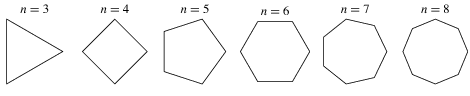
\includegraphics[scale=0.60]{images/regularPolygons}
%\input{regularPolygons}
\caption{Regular polygons}
\label{fig:regularPolygons}
\end{figure}

Write a program that takes $n$ and a radius $r$ as inputs and computes the points
of a regular $n$-sided polygon centered at the origin $(0,0)$.  Each point should be distance $r$
from the origin and the first point should lie on the positive $x$-axis.  Each subsequent point should be
at an angle $\theta$ equal to $\frac{2\pi}{n}$ from the previous point.  Recall that given the
polar coordinates $\theta, r$ we can convert to cartesian coordinates $(x, y)$ using the following.
$$\begin{array}{rcl}
 x & = & r \cdot \cos{\theta} \\
 y & = & r \cdot \sin{\theta}
\end{array}$$
Your program should be robust enough to check for invalid inputs.  If invalid, an error message should
be printed and the program should exit.

For example, running your program with $n = 5, r = 6$ should produce the points of a 
pentagon with ``radius'' $6$.  The output should look something like:

\begin{minted}{text}
Regular 5-sided polygon with radius 6.0:
(6.0000, 0.0000)
(1.8541, 5.7063)
(-4.8541, 3.5267)
(-4.8541, -3.5267)
(1.8541, -5.7063)
\end{minted}

\end{exer}

\begin{exer}
Let $p_1 = (x_1, y_1)$ and $p_2 = (x_2, y_2)$ be two points in the cartesian plane
which define a \emph{line} segment. Suppose we travel along this line starting at $p_1$ 
taking $n$ steps that are an equal distance apart until we  reach $p_2$.  We wish to know 
which points correspond to each of these steps and which step along this path is \emph{closest} 
to anther point $p_3 = (x_3, y_3)$.  Recall that the distance between two points can be 
computed using the Euclidean distance formula:
  $$\delta = \sqrt{(x_1 - x_2)^2 + (y_1-y_2)^2}$$
Write a program that takes three points and an integer $n$ as inputs and
outputs a sequence of points along the line defined by $p_1, p_2$ that are distance 
$\frac{\delta}{n}$ apart from each other.  It should also indicate which of these
computed points is the closest to the third point.  For example, the execution of your program 
with inputs $0, 2, -5.5, 7.75, -2, 3, 10$
should produce output that looks something like:

\begin{minted}{text}
(0.00, 2.00) to (-5.50, 7.75) distance: 7.9569
(0.00, 2.00)
(-0.55, 2.58)
(-1.10, 3.15)
(-1.65, 3.72)  <-- Closest point to (-2, 3)
(-2.20, 4.30)
(-2.75, 4.88)
(-3.30, 5.45)
(-3.85, 6.02)
(-4.40, 6.60)
(-4.95, 7.17)
(-5.50, 7.75)
\end{minted}
\end{exer}

\begin{exer}
The natural log of a number $x$ is usually computed using some numerical
approximation method.  One such method is to use the following Taylor series.
  $$\ln{x} = (x-1) - \frac{(x-1)^2}{2} + \frac{(x-1)^3}{3} - \frac{(x-1)^4}{4} + \cdots$$
However, this only works for $|x-1| \leq 1$ (except for $x=0$) and diverges otherwise.  
For $x$ such that $|x| > 1$, we can use the series
  $$\ln{\frac{y}{y-1}} = \frac{1}{y} + \frac{1}{2y^2} + \frac{1}{3y^3} + \cdots$$
where $y = \frac{x}{x-1}$.  Of course such an infinite computation cannot be performed
by a computer.  Instead, we approximate $\ln{x}$ by computing the series out to a finite number
of terms, $n$.  Your program should print an error message and exit for $x \leq 0$; otherwise it should use the 
first series for $0 < x \leq 1$ and the second for $x > 1$.

Another series that has better convergence properties and works for any range of $x$
is as follows
 $$\ln{x} = \ln{\frac{1+y}{1-y}} = 2y\left(1 + \frac{1}{3}y^2 + \frac{1}{5}y^4 + \frac{1}{7}y^6 \cdots\right)$$
where $y = \frac{(x-1)}{(x+1)}$.

You will write a program that approximates $\ln{x}$ using these two methods computed to
$n$ terms.  You will also compute the error of each method by comparing the approximated
value to the standard math library's \mintinline{c}{log} function.

Your program should accept $x$ and $n$ as inputs.  It should be robust enough to
reject any invalid inputs ($\ln{x}$ is not defined for $x = 0$ you may also print an error for any
negative value; $n$ must be at least one).  It will then compute an approximation using both
methods and print the relative error of each method.

For example, the execution of your program with inputs $3.1415, 6$ should 
produce output that looks something like:

\begin{minted}{text}
Taylor Series: ln(3.1415) ~= 1.11976  
  Error: 0.02494
Other Series:  ln(3.1415) ~= 1.14466  
  Error: 0.00004
\end{minted}
\end{exer}

\begin{exer}
There are many different numerical methods to compute the square root of a number.  In
this exercise, you will implement several of these methods.

\begin{enumerate}
  \item[(a)] The Exponential Identity Method involves the following identity:
           $$\sqrt{x} = e^{\frac{1}{2}\ln{(x)}}$$
	Which assumes the use of built-in (or math-library) functions for $e$ and the natural log, $\ln$.
  \item[(b)] The Babylonian Method involves iteratively computing the following recurrence:
	$$a_{i} = \frac{1}{2}\left( a_{i-1} + \frac{x}{a_{i-1}} \right)$$
	where $a_1 = 1.0$.  Computation is repeated until $|a_{i} - a_{i-1}| \leq \delta$ where 
	$\delta$ is some small constant value.
  \item[(c)] A method developed for one of the first electronic computers (EDSAC \cite{WilkesWheelerGill1952}) involves the following iteration.
	Let $a_0 = x$, $c_0 = x-1$.  Then compute
	$$\begin{array}{rcl}
	    a_{i+1} & = & a_i - \frac{a_ic_i}{2} \\
	    c_{i+1} & = & \frac{c_i^2(c_i - 3)}{4} 
 	\end{array}$$
	The iteration is performed for as many iterations as specified ($n$), or until the change in $a$ is negligible.
	The resulting value for $a$ is used as an approximation for $\sqrt{x} \approx a$.
	However, this method only works for values of $x$ such that $0 < x < 3$.  
	We can easily overcome this by \emph{scaling} $x$ by some power of 4 so that
	the scaled value of $x$ satisfies $\frac{1}{2} \leq x < 2$.  After applying the method we
	can then scale back up by the appropriate value of $2$ (since $\sqrt{4} = 2$).  
\end{enumerate}

Write a program to compute the square root of an input number using these methods and compare your results.
\end{exer}

\begin{exer}
There are many different numerical methods to compute the natural logarithm of a number, $\ln{x}$.  
In this exercise, you will implement several of these methods.

\begin{enumerate}
  \item[(a)] A formula version approximates the natural logarithm as:
  	$$\ln(x) \approx \frac{\pi}{2M(1, 4/s)} -m\ln(2)$$
	Where $M(a, b)$ is the \emph{arithmetic-geometric} mean and $s = x2^m$.  In this formula, 
	$m$ is a parameter (a larger $m$ provides more precision). 	
  \item[(b)] The standard Taylor Series for the natural logarithm is:
  	$$\ln(x) = \sum_{n=1}^\infty \frac{(-1)^{n+1}}{n} (x-1)^n$$
	As we cannot compute an infinite series, we will simply compute the series to the first $m$ terms.
	Also note that this series is not convergent for values $x > 1$
  \item[(c)] Borchardt's algorithm is an iterative method that works as follows. Let
  	$$a_0 = \frac{1+x}{2} \quad\quad b_0 =\sqrt{x}$$
	Then repeat:
	$$\begin{array}{rcl}
	  a_{k+1} & = & \frac{a_k + b_k}{2} \\
	  b_{k+1} & = & \sqrt{a_{k+1}b_k} \\
	  \end{array}$$
	until the absolute difference between $a_k, b_k$ is small; that is $|a_k - b_k| < \epsilon$.
	Then the logarithm is approximated as
	$$\ln(x) \approx 2 \frac{x-1}{a_k+b_k}$$
  \item[(d)] Newton's method works if $x$ is sufficiently close to 1.  It works by setting $y_0 = 1$ and then
  	computing
	$$y_{n+1} = y_n + 2 \frac{x-e^{y_n}}{x+e^{y_n}}$$
	The iteration is performed $m$ times.  
\end{enumerate}	

To ensure that some of the methods above work, you may need to \emph{scale} the
number $x$ to be as close as possible to 1.  One way to do this is to divide or multiply 
by $e$ until $x$ is close to 1.  Suppose we divided by $e$ $k$ times; 
that is $x = z \cdot e^k$ where $z$ is close to 1.  Then 
  $$\ln(x) = \ln(z \cdot e^k) = \ln(z) + \ln(e^k) = \ln(z) + k$$
Thus, we can apply the methods above to Newton's method to $z$ and add $k$ to the 
result to get $\ln(x)$.  A similar trick can be used to ensure that the Taylor Series method is
convergent.
\end{exer}



%CHAPTER: Functions
\chapter{Functions}
\index{functions}
%!TEX root = ComputerScienceOne.tex

\label{chapter:functions}

%Introduction/Motivation

In mathematics, a function is a mapping from a set of \emph{inputs}
to a set of \emph{outputs} such that each input is mapped to exactly one
output.  For example, the function 
  $$f(x) = x^2$$
maps numeric values to their squares.  The input is a variable $x$.  When
we assign an actual value to $x$ and evaluate the function, then the function
has a value, its output.  For example, setting $x = 2$ as input, the output
would be $2^2 = 4$.  Mathematical functions can have multiple inputs, 
  $$f(x,y) = x^2 + y^2 \quad f(\beta, y, z) = 2x + 3y - 4z$$
But will still only ever have \emph{one} output value.

In programming languages, a \gls{function} (sometimes called subroutine 
or procedure) can take multiple inputs and produce one output value.  We've 
already seen some examples of these functions.  For example, most languages 
provide a math library that you can use to evaluate the square root or 
sine of a value $x$.  We've also seen some functions with multiple input 
values such as the ``power'' function that allows you to compute $f(x, y) = x^y$.
The main entry point to many programs is defined by a main function.

More formally, a function is a sequence of instructions (code) that is 
packaged into a \emph{unit} that can be reused.  A function performs 
a specific task: given a number of inputs, it performs some sequence 
of operations (executes some code) and ``returns'' (outputs) a result.
The output can be captured into a variable or other expression by 
whatever code \emph{invoked} or ``called'' the function.

Defining and using functions in programming has numerous advantages.
The most obvious advantage is that it allows you a way to \emph{organize} 
code.  By separating a program it into distinct units code it is more organized 
and it is clearer what each piece or segment of code does.  This also 
facilitates \gls{top-down design}: one way to approach a problem is to 
split it up into a series of subproblems until each subproblem is either trivial 
to deal  with, or an existing, ``off-the-shelf'' solution already exists for it.
Functions may be the logical unit for each subproblem.  

Another advantage is that by organizing code into functions, those functions 
can be \emph{reused} in multiple places either in your program/project 
or even in other programs/projects.  A prime example of this are the standard
libraries available in most programming languages that provide functions
to perform standard input/output or mathematical functions.  These standard
libraries provide functions that are used by thousands of different programs
across multiple different platforms.

Functions also form an \emph{isolated} unit of code.  This allows for 
better and easier \emph{testing}.  By isolating pieces of code, we can 
rigorously test those pieces of code by themselves without worrying 
about the larger program or contexts.  

Finally, functions facilitates \gls{procedural abstraction}.  Placing code 
into functions allows you to abstract the details of how the function computes 
its answer.  As an example: consider a standard math library's square root
function: it may use some interpolation method, a Taylor series, or some 
other method entirely to compute the square root of a given number.  
However, by putting this functionality into a function, we, as programmers, 
do not need to concern ourselves about these details.  Instead, we simply 
\emph{use} the function, allowing us to focus on the larger issues at hand 
in our program.

\section{Defining \& Using Functions}

Like variables, many programming languages may require that you, in 
some way, declare the function before you can use it.  A function
declaration may simply include a description of the function's input/output
and name.  A function declaration may require require you to define
the function's body at the same time or separately.  Functions can also
have scope: some areas of the code may be able to ``see'' the function
or know about it and be able to invoke the function while other areas of
the code may \emph{not} be able to see the function and therefore may
not be able to invoke it.  

Some interpreted programming languages use function \gls{hoisting} which allows
you to use/invoke functions \emph{before} you declare them.  This works
because the interpreter does an initial scan of the code and
identifies all function declarations.  Only after it has ``hoisted'' all functions
into scope does it start to execute the program.  Thus, a function declaration
can appear \emph{after} it has been used and it will still work.

\subsection{Function Signatures}

A function is usually defined by its \gls{signature}: every function can be
identified by its name (also called an \emph{identifier}), its list of 
\emph{input parameters}, and its \emph{output}.  A function signature
allows the programming language to uniquely identify each function
so that when you invoke a function there is no ambiguity in which function
should be called.

\begin{algorithm}[H]
\Fn{sum(a, b)}{
  $x \leftarrow a + b$ \;
  return $x$ \;
}
\caption[A function in pseudocode]{A function in pseudocode.  In this case, the name (identifier) of
the function is \emph{sum} and it has two parameters, $a$ and $b$.  Its
body is contained in lines 2--3.  Its return value is indicated by the return
statement on line 3.}
\label{algorithm:function}
\end{algorithm}

A function declaration in pseudocode is presented in Algorithm 
\ref{algorithm:function}.  In the pseudocode, explicit variable types
are omitted, and thus the return type is inferred from the return statement.
In Figure \ref{figure:cFunctionPrototype} we have provided an example
of a function declaration in the C programming language with each
element labeled. 

\begin{figure}[H]
\centering
%\documentclass[12pt]{article}
%\usepackage{tikz}
%\usetikzlibrary{backgrounds}
%\usetikzlibrary{decorations.pathreplacing}
%
%%\usepackage{newfloat}
%\usepackage{minted}
%\setminted{mathescape,
%               linenos,
%               autogobble,
%               frame=none,
%               framesep=2mm,
%               framerule=0.4pt,
%               %label=foo,
%               xleftmargin=2em,
%               xrightmargin=0em,
%               numbersep=10pt, %gap between line numbers and start of line
%               style=default}
%\usepackage{fullpage}
%\begin{document}

\begin{tikzpicture}[framed]

  \node (main) {
{
\mintinline[]{c}{double getDistance(double x1, double y1, double x2, double y2);}
}
  
  };

%  \node (formatstring) at (-5,2) {Format String};

%  \node (placeholders) at (1,-1.5) {Placeholders};
 % \draw[->] (placeholders.north) -- ([xshift=-.70cm,yshift=0.15cm]main.south);
  %\draw[->] (placeholders.north) -- ([xshift=3.7cm,yshift=0.2cm]main.south);
  
  \draw [decorate,decoration={brace,amplitude=10pt},xshift=-4pt,yshift=0pt] ([xshift=-2.65cm]main.north) -- ([xshift=6.25cm]main.north) node [black,midway,yshift=0.65cm] {Parameters};

  \draw [decorate,decoration={brace,mirror,amplitude=5pt},xshift=-4pt,yshift=0pt] ([xshift=-6.75cm]main.south) -- ([xshift=-5.5cm]main.south) node [below,align=center,text width=2cm,black,midway,yshift=-0.25cm] {Return Type};

  \draw [decorate,decoration={brace,mirror,amplitude=5pt},xshift=-4pt,yshift=0pt] ([xshift=-5.25cm]main.south) -- ([xshift=-3.0cm]main.south) node [below,align=center,text width=2cm,black,midway,yshift=-0.25cm] {Identifier (name)};

%\draw[black,fill=black] (placeholders.north) circle (.5pt);

\end{tikzpicture}

%\end{document}

\caption{A function declaration (prototype) in the C programming language
with the return type, identifier, and parameter list labeled.}
\label{figure:cFunctionPrototype}
\end{figure}

Some languages only allow you to use one identifier for one function 
(like variables) while other languages allow you to define multiple functions
with the same identifier as long as the parameter list is different (see
Section \ref{subsection:functionOverloading} below).  In general, like variables, function names
are case sensitive.  Also similar to variables, modern lower camel casing
is used with function names.  

When defining the parameters to a function (its input), you usually provide
a comma delimited list of variable names.  In the case of statically typed
languages, the types of the variable parameters are also specified.  This
order is important as when you invoke the function, the number of inputs
must match the number of parameters in the function declaration.  The 
variable types may also need to match.  In some dynamically typed languages, 
you may be able to call functions with different types or you may be able
to omit some of the parameters (see Section \ref{subsection:optionalParameters}
below).

Similarly, the return type of the function may need to be specified in 
statically typed languages while with dynamic languages, functions may
conditionally return different types.  We generally refer to the ``return value''
or ``return type'' because when a function is done executing, it ``returns''
the control flow back to the line of code that invoked it, returning its
computed value.

You can also define functions that may not have any inputs or may not
have any output.  Some languages use the keyword \mintinline{text}{void} 
to indicate no return value and such functions are known as ``void 
functions.''  When a function doesn't have any input values, its parameter
list is usually empty.

The function signature may then be accompanied by the function \emph{body}
which contains the actual code that specifies what the function does.  
Typically the function body is demarcated with opening and closing curly
brackets, \mintinline{text}{{ ... }}.  Within the function you can generally
write any valid code including declaring variables.  When you declare a 
variable inside a function, however, it is \emph{local} to that function.
That is, the variable's scope is only defined within the function.  A local
variable cannot be accessed outside the function, indeed the local
variable does not usually survive when the function ends its
execution and returns control back to line of code that called it. 
Function parameters are essentially locally scoped variables as well 
and can usually be treated as such.

\subsection{Calling Functions}

When a function has been defined and is in scope, you can \emph{invoke}
or ``call'' the function by coding the function name and providing the input
parameters which can typically be either variables or literals.  When
provided as inputs, parameters are referred to as \emph{arguments}
to the function.  The arguments are typically provided as a comma delimited
list and placed inside parentheses.  

Invoking a function changes the usual flow of control.  When invoked, control
is handed over to the function.  When the function finishes executing the
code in its body, control flow returns to the point in the code that invoked it.
It is common for a program to be written so that a function calls another function
and that function calls another.  This can form a deep chain of function calls in 
which the flow of control is transferred multiple times.  Upon the completion
of each function, control is returned back to the function that called it, 
referred to as the \emph{calling function}.

If a function returns a value it can either be captured in a variable using an
assignment operator or by using it in an expression.  

\begin{algorithm}[H]
$a \leftarrow 10$ \;
$b \leftarrow 20$ \;
$c \leftarrow sum(a, b)$ \;
\caption[Using a function]{Using a function.  We invoke a function by 
indicating its name (identifier) and passing it arguments.}
\label{algorithm:functionCall}
\end{algorithm}

\subsection{Organizing}   

Functions provide code organization, but functions themselves should also
be organized.  We've seen this with standard libraries.  Functions that provide
basic input/output are all grouped together into one library.  
Functions that involve math functions are grouped together into a math library.

Some languages allow you to define and ``import'' individual libraries 
which organize similar functions together.  Some languages do this by 
collecting functions into ``utility'' classes or \emph{modules}.  Only when
you import these modules do the functions come into scope and can be
used in your code.  If you do not import these modules, then the functions
are out of scope and cannot be used.  

In some languages, functions, once imported, are part of the \emph{global
scope} and can be ``seen'' by any part of the code.  This can cause
\emph{conflicts}: if you import modules from two different libraries each
with different functions that have the same name or signature, then 
the two function definitions may be in conflict or it may make your
code ambiguous as to which function you intend to invoke.  This is
sometimes referred to as ``polluting the namespace.''  There are
several techniques that can avoid this situation.  Some languages allow
you to place functions into a \emph{namespace} to keep functions with
the same name in different ``spaces.''  Other languages allow you to 
place functions into different classes and then invoke them by explicitly
specifying \emph{which} class's function you want to call.  Yet other
languages don't have great support for function organization and it is
the library designer's responsibility to avoid naming conflicts, typically
by adding a library-specific prefix to every function.

\section{How Functions Work}

To understand how functions work in practice, it is necessary to 
understand how a program operates at a lower level.  In particular,
each program has a \gls{program stack} (also called a call stack).  
A \gls{stack} is a data structure that holds elements in a \gls{lifoLabel}
manner.  Elements are added to the ``top'' of the stack in an operation
called \emph{push} and elements can be removed from the top
of the stack in an operation called \emph{pop}.  In general, elements 
cannot be inserted or removed from the middle or ``bottom'' of the 
stack.

In the context of a program, a call stack is used to keep track of the 
flow of control.  Depending on the operating system, compiler and architecture, 
the details of how elements are stored in the program stack may 
vary.  However, in general when a program begins, the operating 
system loads it into memory at the bottom of the call stack.  Global 
variables (static data) are stored on top of the main program.  Each
time a function is called, a new \emph{stack frame} is placed on
top of the stack.  This frame contains enough space to hold values
for the arguments passed to the function, local variables declared
and used by the function, as well as a space for a return value and
a return \emph{address}.  The return address is a memory location
that the program should return to after the execution of the function.
That way, when the function finishes its execution, the stack frame
can be removed (popped) and the lower stack frame of the calling
function is preserved.  This is a very efficient way to keep track of
the flow of control in a program.  As function calls function calls
another function, each stack frame is preserved by pushing a new
one on top of the program stack.

Each time a function terminates execution and returns, the removal
of the stack frame means that all local variables go \emph{out of
scope}.  Thus, variables that are local to a function are not accessible
outside the function.

To illustrate, consider the following snippet of C code.  The \mintinline{c}{main()}
function invokes the \mintinline{c}{average()} function which in 
turn invokes the \mintinline{c}{sum()} function.  Each invocation 
creates a new stack frame on top of the last in the program stack
which is depicted in Figure \ref{figure:programStack}.

\begin{minted}{c}
double sum(double a, double b) {
  double x = a + b;
  return x;
}

double average(double a, double b) {
  double y = sum(a, b) / 2.0;
  return y;
}

int main(int argc, char **argv) {
  double n = 10.0;
  double m = 16.0;
  double ave = average(n, m);
  printf("average = %f\n", ave);
  return 0;
}
\end{minted}

\begin{figure}[!h]
\centering
%\documentclass[12pt]{article}
%\usepackage{tikz}
%\usepackage{minted}
%\usetikzlibrary{decorations.pathreplacing}
%\usetikzlibrary{fadings}
%\usepackage{fullpage}
%\begin{document}
%\begin{figure}
%\centering

\begin{tikzpicture}[auto,scale=0.80,transform shape,every node/.style={text centered, text width=5.5cm}]

\node [above left] (bottom) at (0,0) {Bottom of the stack (high memory)};
\node [below left] (top) at (0,15.5) {Top of the stack (low memory)};

\draw (6,18.5) -- (6, 15.5);
\draw[path fading=north] (0,15.5) -- (0, 18.5);
\node [above] (unused) at (3, 16) {Unused stack space};

\draw[fill=blue!10!white] (0, 0) rectangle (6,2);
\node [above] (pc) at (3,0) {Program Code};

\draw[fill=yellow!10!white] (0, 2) rectangle (6,3.5);
\node [above] (globals) at (3,2) {Global Variables \\ Static Content};

\draw[fill=green!30!white] (0, 3.5) rectangle (6,7.5);
\node [above] (main) at (3,3.5) {arguments \mintinline{c}{argc, argv}};
\draw[dashed] (0, 5) -- (6, 5);
\node [above] (mainvar) at (3,5) {return address, value (\mintinline{c}{0})};
\draw[dashed] (0, 6) -- (6, 6);
\node [above] (mainvar2) at (3,6) {local variables \mintinline{c}{n, m, ave}};
\draw [decorate,decoration={brace,amplitude=10pt,mirror},xshift=4pt,yshift=0pt] (6, 3.5) -- (6, 6.5+1) node [align=left,black,midway,xshift=6.25cm]  {\texttt{main()} stack frame};


\draw[fill=green!20!white] (0, 3.5+4) rectangle (6,7.5+4);
\node [above] (main) at (3,3.5+4) {arguments \mintinline{c}{a, b}};
\draw[dashed] (0, 5+4) -- (6, 5+4);
\node [above] (mainvar) at (3,5+4) {return address, value (\mintinline{c}{12.5})};
\draw[dashed] (0, 6+4) -- (6, 6+4);
\node [above] (mainvar2) at (3,6+4) {local variables \mintinline{c}{y}};
\draw [decorate,decoration={brace,amplitude=10pt,mirror},xshift=4pt,yshift=0pt] (6, 3.5+4) -- (6, 7.5+4) node [align=left,black,midway,xshift=6.25cm]  {\texttt{average()} stack frame};


\draw[fill=green!10!white] (0, 3.5+8) rectangle (6,7.5+8);
\node [above] (main) at (3,3.5+8) {arguments \mintinline{c}{a, b}};
\draw[dashed] (0, 5+8) -- (6, 5+8);
\node [above] (mainvar) at (3,5+8) {return address, value (\mintinline{c}{26.0})};
\draw[dashed] (0, 6+8) -- (6, 6+8);
\node [above] (mainvar2) at (3,6+8) {local variables \mintinline{c}{x}};
\draw [decorate,decoration={brace,amplitude=10pt,mirror},xshift=4pt,yshift=0pt] (6, 3.6+8) -- (6, 7.6+8) node [align=left,black,midway,xshift=6.25cm]  {\texttt{sum()} stack frame};


\end{tikzpicture}


%\end{document}


\caption[Program Stack]{Program Stack.  At the bottom we have the program's code, followed by
static content such as global variables.  Each function call has its own stack frame along with
its own arguments and local variables.  In particular, the variable arguments \mintinline{c}{a} and
\mintinline{c}{b} in two different stack frames are completely different variables.  Upon returning
from the \mintinline{c}{sum()} function call, the top-most stack frame would be popped and removed, 
returning to the code for the \mintinline{c}{average()} function via the return address.
The stack is depicted bottom-up with high memory at the bottom and low memory at the
top, but this may differ depending on the architecture.}
\label{figure:programStack}
\end{figure}


%Recall that everything in a program is stored in memory; variables, 
%constants, values, etc.  Of course, this \emph{includes} the program
%itself.  Each function in a program is stored at some memory address

\subsection{Call By Value}

When a function is invoked, arguments are passed to it.  When you
invoke a function you can pass it variables as arguments.  However,
variables themselves are not passed to the function, but instead the
values \emph{stored} in the variables at the time that you call the
function are passed to the function.  This mechanism is known as 
\gls{call by value} and the variable values are \emph{passed by value}
to the function.

Recall that the arguments passed to a function are placed in a new
stack frame for that function.  Thus, in reality \emph{copies} of the
values of the variables are passed to the function.  Any changes to
the parameters inside the function have \emph{no effect} on the
original variables that were ``passed'' to the function when it was 
invoked.  

%(TODO: is there a more pseudocody way of doing this?)
To illustrate, consider the following C code.  We have a function \mintinline{c}{sum}
that takes two integer parameters \mintinline{c}{a} and \mintinline{c}{b}
which are passed by value.  Inside \mintinline{c}{sum}, we create another
variable \mintinline{c}{x} which is the sum of the two passed variables.
We then \emph{change} the value of the first variable, \mintinline{c}{a}
to \mintinline{c}{10}.  Elsewhere in the code we call \mintinline{c}{sum}
on two variables, \mintinline{c}{n}, \mintinline{c}{m} with values
5 and 15 respectively.  The invocation of the function \mintinline{c}{sum} 
means that the two values, 5 and 15, stored in the variables are
copied into a new stack frame.  Thus, changing the value to the
first parameter \emph{changes the copy} and has no effect on the
variable \mintinline{c}{n}.  At the end of this code snippet \mintinline{c}{n}
retains its original value of 5.  The program stack frames are depicted
in Figure \ref{figure:PassByValue}.

\begin{minted}{c}
int sum(int a, int b) {
  int x = a + b;
  a = 10;
  return x;
}

...

int n = 5;
int m = 15;
int k = sum(n, m);
\end{minted}

%\documentclass[12pt]{scrbook}
%
%\usepackage{tikz}
%\usepackage{minted}
%\usetikzlibrary{decorations.pathreplacing}
%\usetikzlibrary{patterns}
%
%\usepackage{fullpage}
%\usepackage{subfigure}
%\begin{document}
%
%
%Lorem Ipsum is simply dummy text of the printing and typesetting industry. Lorem Ipsum has been the industry's standard dummy text ever since the 1500s, when an unknown printer took a galley of type and scrambled it to make a type specimen book. It has survived not only five centuries, but also the leap into electronic typesetting, remaining essentially unchanged. It was popularised in the 1960s with the release of Letraset sheets containing Lorem Ipsum passages, and more recently with desktop publishing software like Aldus PageMaker including versions of Lorem Ipsum.
%

\begin{figure}
\centering

\subfigure[Upon invocation of the \mintinline{c}{sum()} function, a new stack frame is created which holds
the parameters and local variable.  The parameter variables \mintinline{c}{a} and \mintinline{c}{b}
are \emph{distinct} from the original argument variables \mintinline{c}{n} and \mintinline{c}{m}.]{

\begin{tikzpicture}[auto,scale=.75,transform shape,every node/.style={text centered}]

%\draw[path fading=north] (0,15.5) -- (0, 18.5);

\draw[fill=green!10!white] (0, 0) rectangle (3, 1.2em);
\node [above] (a1) at (1.5,0) {\texttt{0x0010}};
\draw[fill=green!10!white] (3, 0) rectangle (6, 1.2em);
\node [above] (a2) at (4.5,0) {\texttt{n = 5}};

\draw[fill=green!10!white] (0, 0+1.2em) rectangle (3, 2.4em);
\node [above] (b1) at (1.5,0+1.2em) {\texttt{0x0014}};
\draw[fill=green!10!white] (3, 0+1.2em) rectangle (6, 2.4em);
\node [above] (b2) at (4.5,0+1.2em) {\texttt{m = 10}};

\draw[fill=green!10!white] (0, 0+2.4em) rectangle (3, 3.6em);
\node [above] (b1) at (1.5,0+2.4em) {\texttt{0x0018}};
\draw[fill=green!10!white] (3, 0+2.4em) rectangle (6, 3.6em);
\node [above] (b2) at (4.5,0+2.4em) {\texttt{k}};

\path [top color=white, bottom color=green!10!white] (0,3.625em) rectangle (6,6em);

\fill [top color=white, bottom color=black] (-0.0075,3.6em) rectangle (.02em,6em);
\fill [top color=white, bottom color=black] (5.9925,3.6em) rectangle (6.0075,6em);
\fill [top color=white, bottom color=black] (2.9925,3.6em) rectangle (3.0075,6em);
      
%\draw[top color=white,
%      bottom color=green!10!white]
% (0,3.6em) rectangle (6,6em);
 
%\draw[bottom color=transparent!0,top color=transparent!100] (0,3.6em) -- (0,6em);
%\draw[] (6cm,3.6em) -- (6cm,6em);

%\draw[dashed] (0, 5) -- (6, 5);
%\node [above] (mainvar) at (3,5) {return address, value (\mintinline{c}{0})};
%\draw[dashed] (0, 6) -- (6, 6);
%\node [above] (mainvar2) at (3,6) {local variables \mintinline{c}{n, m, ave}};
\draw [decorate,decoration={brace,amplitude=5pt},xshift=-4pt,yshift=0pt] (0, 0) -- (0, 3.6em) node [text width=3cm,align=center,black,midway,xshift=-.25cm]  {calling function stack frame};


\path [top color=green!10!white, bottom color=white] (0,3) rectangle (6,5);
\fill [top color=black, bottom color=white] (-0.0075,3.5) rectangle (.01,5);
\fill [top color=black, bottom color=white] (2.9925,3.5) rectangle (3.01,5);
\fill [top color=black, bottom color=white] (5.9925,3.5) rectangle (6.01,5);

\draw[fill=green!10!white] (0, 4.5) rectangle (3, 5);
\node [above] (aa1) at (1.5,4.5) {\texttt{0x0080}};
\draw[fill=green!10!white] (3, 4.5) rectangle (6, 5);
\node [above] (aa2) at (4.5,4.5) {\texttt{a = 5}};

\draw[fill=green!10!white] (0, 5) rectangle (3, 5.5);
\node [above] (bb1) at (1.5,5) {\texttt{0x0084}};
\draw[fill=green!10!white] (3, 5) rectangle (6, 5.5);
\node [above] (bb2) at (4.5,5) {\texttt{b = 15}};

\draw[fill=green!10!white] (0, 5.5) rectangle (3, 6);
\node [above] (cc1) at (1.5,5.5) {\texttt{0x0088}};
\draw[fill=green!10!white] (3, 5.5) rectangle (6, 6);
\node [above] (cc2) at (4.5,5.5) {\texttt{x = 20}};

\draw [decorate,decoration={brace,amplitude=5pt},xshift=-4pt,yshift=0pt] (0, 4.5) -- (0, 6) node [text width=3cm,align=center,black,midway,xshift=-.25cm]  {\mintinline{c}{sum()} stack frame};

\node (dots) at (3, 3.15) {$\vdots$};

\path [top color=white, bottom color=green!10!white] (0,6.01) rectangle (6,7);

\fill [top color=white, bottom color=black] (-0.00725,6) rectangle (.0075,7);
\fill [top color=white, bottom color=black] (5.9925,6) rectangle (6.0075,7);
\fill [top color=white, bottom color=black] (2.9925,6) rectangle (3.0075,7);


\end{tikzpicture}
}~~~~\subfigure[The change to the variable \mintinline{c}{a} in the \mintinline{c}{sum()}
function changes the parameter variable, but the original variable \mintinline{c}{n}
is unaffected.]{

\begin{tikzpicture}[auto,scale=.75,transform shape,every node/.style={text centered}]

%\draw[path fading=north] (0,15.5) -- (0, 18.5);

\draw[fill=green!10!white] (0, 0) rectangle (3, 1.2em);
\node [above] (a1) at (1.5,0) {\texttt{0x0010}};
\draw[fill=green!10!white] (3, 0) rectangle (6, 1.2em);
\node [above] (a2) at (4.5,0) {\texttt{n = 5}};

\draw[fill=green!10!white] (0, 0+1.2em) rectangle (3, 2.4em);
\node [above] (b1) at (1.5,0+1.2em) {\texttt{0x0014}};
\draw[fill=green!10!white] (3, 0+1.2em) rectangle (6, 2.4em);
\node [above] (b2) at (4.5,0+1.2em) {\texttt{m = 10}};

\draw[fill=green!10!white] (0, 0+2.4em) rectangle (3, 3.6em);
\node [above] (b1) at (1.5,0+2.4em) {\texttt{0x0018}};
\draw[fill=green!10!white] (3, 0+2.4em) rectangle (6, 3.6em);
\node [above] (b2) at (4.5,0+2.4em) {\texttt{k}};

\path [top color=white, bottom color=green!10!white] (0,3.625em) rectangle (6,6em);

\fill [top color=white, bottom color=black] (-0.0075,3.6em) rectangle (.02em,6em);
\fill [top color=white, bottom color=black] (5.9925,3.6em) rectangle (6.0075,6em);
\fill [top color=white, bottom color=black] (2.9925,3.6em) rectangle (3.0075,6em);
      
%\draw[top color=white,
%      bottom color=green!10!white]
% (0,3.6em) rectangle (6,6em);
 
%\draw[bottom color=transparent!0,top color=transparent!100] (0,3.6em) -- (0,6em);
%\draw[] (6cm,3.6em) -- (6cm,6em);

%\draw[dashed] (0, 5) -- (6, 5);
%\node [above] (mainvar) at (3,5) {return address, value (\mintinline{c}{0})};
%\draw[dashed] (0, 6) -- (6, 6);
%\node [above] (mainvar2) at (3,6) {local variables \mintinline{c}{n, m, ave}};
\draw [decorate,decoration={brace,amplitude=5pt},xshift=-4pt,yshift=0pt] (0, 0) -- (0, 3.6em) node [text width=3cm,align=center,black,midway,xshift=-.25cm]  {calling function stack frame};


\path [top color=green!10!white, bottom color=white] (0,3) rectangle (6,5);
\fill [top color=black, bottom color=white] (-0.0075,3.5) rectangle (.01,5);
\fill [top color=black, bottom color=white] (2.9925,3.5) rectangle (3.01,5);
\fill [top color=black, bottom color=white] (5.9925,3.5) rectangle (6.01,5);

\draw[fill=green!10!white] (0, 4.5) rectangle (3, 5);
\node [above] (aa1) at (1.5,4.5) {\texttt{0x0080}};
\draw[fill=green!10!white] (3, 4.5) rectangle (6, 5);
\node [above] (aa2) at (4.5,4.5) { \color{red}{\texttt{a = 10}}};

\draw[fill=green!10!white] (0, 5) rectangle (3, 5.5);
\node [above] (bb1) at (1.5,5) {\texttt{0x0084}};
\draw[fill=green!10!white] (3, 5) rectangle (6, 5.5);
\node [above] (bb2) at (4.5,5) {\texttt{b = 15}};

\draw[fill=green!10!white] (0, 5.5) rectangle (3, 6);
\node [above] (cc1) at (1.5,5.5) {\texttt{0x0088}};
\draw[fill=green!10!white] (3, 5.5) rectangle (6, 6);
\node [above] (cc2) at (4.5,5.5) {\texttt{x = 20}};

\draw [decorate,decoration={brace,amplitude=5pt},xshift=-4pt,yshift=0pt] (0, 4.5) -- (0, 6) node [text width=3cm,align=center,black,midway,xshift=-.25cm]  {\mintinline{c}{sum()} stack frame};

\node (dots) at (3, 3.15) {$\vdots$};

\path [top color=white, bottom color=green!10!white] (0,6.01) rectangle (6,7);

\fill [top color=white, bottom color=black] (-0.00725,6) rectangle (.0075,7);
\fill [top color=white, bottom color=black] (5.9925,6) rectangle (6.0075,7);
\fill [top color=white, bottom color=black] (2.9925,6) rectangle (3.0075,7);


\end{tikzpicture}

}

\subfigure[When the \mintinline{c}{sum()} function finishes execution, its stack frame
is removed and the variables \mintinline{c}{a}, \mintinline{c}{b}, and \mintinline{c}{x} are
no longer valid.  The return value 20 is stored in another return value location.]{


\begin{tikzpicture}[auto,scale=.75,transform shape,every node/.style={text centered}]

%\draw[path fading=north] (0,15.5) -- (0, 18.5);

\draw[fill=green!10!white] (0, 0) rectangle (3, 1.2em);
\node [above] (a1) at (1.5,0) {\texttt{0x0010}};
\draw[fill=green!10!white] (3, 0) rectangle (6, 1.2em);
\node [above] (a2) at (4.5,0) {\texttt{n = 5}};

\draw[fill=green!10!white] (0, 0+1.2em) rectangle (3, 2.4em);
\node [above] (b1) at (1.5,0+1.2em) {\texttt{0x0014}};
\draw[fill=green!10!white] (3, 0+1.2em) rectangle (6, 2.4em);
\node [above] (b2) at (4.5,0+1.2em) {\texttt{m = 10}};

\draw[fill=green!10!white] (0, 0+2.4em) rectangle (3, 3.6em);
\node [above] (b1) at (1.5,0+2.4em) {\texttt{0x0018}};
\draw[fill=green!10!white] (3, 0+2.4em) rectangle (6, 3.6em);
\node [above] (b2) at (4.5,0+2.4em) {\color{black}{\texttt{k}}};

\path [top color=white, bottom color=green!10!white] (0,3.625em) rectangle (6,6em);

\fill [top color=white, bottom color=black] (-0.0075,3.6em) rectangle (.02em,6em);
\fill [top color=white, bottom color=black] (5.9925,3.6em) rectangle (6.0075,6em);
\fill [top color=white, bottom color=black] (2.9925,3.6em) rectangle (3.0075,6em);
      
%\draw[top color=white,
%      bottom color=green!10!white]
% (0,3.6em) rectangle (6,6em);
 
%\draw[bottom color=transparent!0,top color=transparent!100] (0,3.6em) -- (0,6em);
%\draw[] (6cm,3.6em) -- (6cm,6em);

%\draw[dashed] (0, 5) -- (6, 5);
%\node [above] (mainvar) at (3,5) {return address, value (\mintinline{c}{0})};
%\draw[dashed] (0, 6) -- (6, 6);
%\node [above] (mainvar2) at (3,6) {local variables \mintinline{c}{n, m, ave}};
\draw [decorate,decoration={brace,amplitude=5pt},xshift=-4pt,yshift=0pt] (0, 0) -- (0, 3.6em) node [text width=3cm,align=center,black,midway,xshift=-.25cm]  {calling function stack frame};


\path [top color=green!10!white, bottom color=white] (0,3) rectangle (6,5);
\fill [top color=black, bottom color=white] (-0.0075,3.5) rectangle (.01,5);
\fill [top color=black, bottom color=white] (2.9925,3.5) rectangle (3.01,5);
\fill [top color=black, bottom color=white] (5.9925,3.5) rectangle (6.01,5);

\draw[fill=green!10!white] (0, 4.5) rectangle (3, 5);
\node [above] (aa1) at (1.5,4.5) {\texttt{0x0080}};
\draw[fill=green!10!white] (3, 4.5) rectangle (6, 5);
\node [above] (aa2) at (4.5,4.5) {\texttt{a = 10}};

\draw[fill=green!10!white] (0, 5) rectangle (3, 5.5);
\node [above] (bb1) at (1.5,5) {\texttt{0x0084}};
\draw[fill=green!10!white] (3, 5) rectangle (6, 5.5);
\node [above] (bb2) at (4.5,5) {\texttt{b = 15}};

\draw[fill=green!10!white] (0, 5.5) rectangle (3, 6);
\node [above] (cc1) at (1.5,5.5) {\texttt{0x0088}};
\draw[fill=green!10!white] (3, 5.5) rectangle (6, 6);
\node [above] (cc2) at (4.5,5.5) {\texttt{x = 20}};

%cross outs: 
\draw[pattern=north west lines, pattern color=blue!50!white] (0,4.5) rectangle (6,6);


\draw [decorate,decoration={brace,amplitude=5pt},xshift=-4pt,yshift=0pt] (0, 4.5) -- (0, 6) node [text width=3cm,align=center,black,midway,xshift=-.25cm]  {\mintinline{c}{sum()} stack frame};

\node (dots) at (3, 3.15) {$\vdots$};

\path [top color=white, bottom color=green!10!white] (0,6.01) rectangle (6,7);

\fill [top color=white, bottom color=black] (-0.00725,6) rectangle (.0075,7);
\fill [top color=white, bottom color=black] (5.9925,6) rectangle (6.0075,7);
\fill [top color=white, bottom color=black] (2.9925,6) rectangle (3.0075,7);


\end{tikzpicture}

}~~~~~\subfigure[The returned value is stored in the variable \mintinline{c}{k} and
the variable \mintinline{c}{n} retains its original value.]{


\begin{tikzpicture}[auto,scale=.75,transform shape,every node/.style={text centered}]

%\draw[path fading=north] (0,15.5) -- (0, 18.5);

\draw[fill=green!10!white] (0, 0) rectangle (3, 1.2em);
\node [above] (a1) at (1.5,0) {\texttt{0x0010}};
\draw[fill=green!10!white] (3, 0) rectangle (6, 1.2em);
\node [above] (a2) at (4.5,0) {\texttt{n = 5}};

\draw[fill=green!10!white] (0, 0+1.2em) rectangle (3, 2.4em);
\node [above] (b1) at (1.5,0+1.2em) {\texttt{0x0014}};
\draw[fill=green!10!white] (3, 0+1.2em) rectangle (6, 2.4em);
\node [above] (b2) at (4.5,0+1.2em) {\texttt{m = 10}};

\draw[fill=green!10!white] (0, 0+2.4em) rectangle (3, 3.6em);
\node [above] (b1) at (1.5,0+2.4em) {\texttt{0x0018}};
\draw[fill=green!10!white] (3, 0+2.4em) rectangle (6, 3.6em);
\node [above] (b2) at (4.5,0+2.4em) {\color{red}{\texttt{k = 20}}};

\path [top color=white, bottom color=green!10!white] (0,3.625em) rectangle (6,6em);

\fill [top color=white, bottom color=black] (-0.0075,3.6em) rectangle (.02em,6em);
\fill [top color=white, bottom color=black] (5.9925,3.6em) rectangle (6.0075,6em);
\fill [top color=white, bottom color=black] (2.9925,3.6em) rectangle (3.0075,6em);
      
%\draw[top color=white,
%      bottom color=green!10!white]
% (0,3.6em) rectangle (6,6em);
 
%\draw[bottom color=transparent!0,top color=transparent!100] (0,3.6em) -- (0,6em);
%\draw[] (6cm,3.6em) -- (6cm,6em);

%\draw[dashed] (0, 5) -- (6, 5);
%\node [above] (mainvar) at (3,5) {return address, value (\mintinline{c}{0})};
%\draw[dashed] (0, 6) -- (6, 6);
%\node [above] (mainvar2) at (3,6) {local variables \mintinline{c}{n, m, ave}};
\draw [decorate,decoration={brace,amplitude=5pt},xshift=-4pt,yshift=0pt] (0, 0) -- (0, 3.6em) node [text width=3cm,align=center,black,midway,xshift=-.25cm]  {calling function stack frame};


\path [top color=green!10!white, bottom color=white] (0,3) rectangle (6,5);
\fill [top color=black, bottom color=white] (-0.0075,3.5) rectangle (.01,5);
\fill [top color=black, bottom color=white] (2.9925,3.5) rectangle (3.01,5);
\fill [top color=black, bottom color=white] (5.9925,3.5) rectangle (6.01,5);

\draw[fill=green!10!white] (0, 4.5) rectangle (3, 5);
\node [above] (aa1) at (1.5,4.5) {\texttt{0x0080}};
\draw[fill=green!10!white] (3, 4.5) rectangle (6, 5);
\node [above] (aa2) at (4.5,4.5) {\texttt{a = 10}};

\draw[fill=green!10!white] (0, 5) rectangle (3, 5.5);
\node [above] (bb1) at (1.5,5) {\texttt{0x0084}};
\draw[fill=green!10!white] (3, 5) rectangle (6, 5.5);
\node [above] (bb2) at (4.5,5) {\texttt{b = 15}};

\draw[fill=green!10!white] (0, 5.5) rectangle (3, 6);
\node [above] (cc1) at (1.5,5.5) {\texttt{0x0088}};
\draw[fill=green!10!white] (3, 5.5) rectangle (6, 6);
\node [above] (cc2) at (4.5,5.5) {\texttt{x = 20}};

%cross outs: 
\draw[pattern=north west lines, pattern color=blue!50!white] (0,4.5) rectangle (6,6);


\draw [decorate,decoration={brace,amplitude=5pt},xshift=-4pt,yshift=0pt] (0, 4.5) -- (0, 6) node [text width=3cm,align=center,black,midway,xshift=-.25cm]  {\mintinline{c}{sum()} stack frame};

\node (dots) at (3, 3.15) {$\vdots$};

\path [top color=white, bottom color=green!10!white] (0,6.01) rectangle (6,7);

\fill [top color=white, bottom color=black] (-0.00725,6) rectangle (.0075,7);
\fill [top color=white, bottom color=black] (5.9925,6) rectangle (6.0075,7);
\fill [top color=white, bottom color=black] (2.9925,6) rectangle (3.0075,7);


\end{tikzpicture}

}

\caption[Demonstration of Pass By Value]{Demonstration of Pass By Value.  Passing variables
by value means that \emph{copies} of the values stored in the variables are provided to the 
function.  Changes to parameter variables do not affect the original variables.}
\label{figure:PassByValue}

\end{figure}




%\end{document}


\subsection{Call By Reference}

Some languages allow you to pass a parameter to a function by
providing its memory address.  Since the memory address is being
provided to the function, the function is able to access the original
variable and manipulate the contents stored at that memory address.
In particular, the function is now able to make changes to the original
variable.  This mechanism is known as \gls{call by reference} and 
the variables are \emph{passed by reference}.

%(TODO: again, can this be done with pseudocode?). 
To illustrate consider the following C code. Here, the variable \mintinline{c}{a}
is passed by reference (\mintinline{c}{b} is still passed by value, 
the \mintinline{c}{*a} and \mintinline{c}{&n} in the following code
are dereferencing and referencing operators respectively.  For
details, see Section \ref{section:cPointers}).  Below when we
invoke the \mintinline{c}{sum} function, we pass not the value
stored in \mintinline{c}{n}, but the memory address of the
variable \mintinline{c}{n}.  Thus, when we change the value of
the variable \mintinline{c}{a} in the function, we are actually 
changing the value of \mintinline{c}{n} (since we have access
to its memory location.  At the conclusion of this snippet of
code, the value stored in \mintinline{c}{n} has been changed to
10.  The program stack frames are depicted in Figure \ref{figure:PassByReference}.

\begin{minted}{c}
int sym(int *a, int b) {
  int x = *a + b;
  *a = 10;
  return x;
}

...

int n = 5;
int m = 15;
int k = sum(&n, m);
\end{minted}

%\documentclass[12pt]{scrbook}
%
%\usepackage{tikz}
%\usepackage{minted}
%\usetikzlibrary{decorations.pathreplacing}
%
%\usetikzlibrary{patterns}
%
%\usepackage{fullpage}
%\usepackage{subfigure}
%\begin{document}
%
%
%Lorem Ipsum is simply dummy text of the printing and typesetting industry. Lorem Ipsum has been the industry's standard dummy text ever since the 1500s, when an unknown printer took a galley of type and scrambled it to make a type specimen book. It has survived not only five centuries, but also the leap into electronic typesetting, remaining essentially unchanged. It was popularised in the 1960s with the release of Letraset sheets containing Lorem Ipsum passages, and more recently with desktop publishing software like Aldus PageMaker including versions of Lorem Ipsum.
%

\begin{figure}
\centering

\subfigure[Upon invocation of the \mintinline{c}{sum()} function, a new stack frame is created which holds
the parameters and local variable.  The parameter variable \mintinline{c}{a} holds
the memory location of the original variable \mintinline{c}{n}.]{

\begin{tikzpicture}[auto,scale=.75,transform shape,every node/.style={text centered}]

%\draw[path fading=north] (0,15.5) -- (0, 18.5);

\draw[fill=green!10!white] (0, 0) rectangle (3, 1.2em);
\node [above] (a1) at (1.5,0) {\texttt{0x0010}};
\draw[fill=green!10!white] (3, 0) rectangle (6, 1.2em);
\node [above] (a2) at (4.5,0) {\texttt{n = 5}};

\draw[fill=green!10!white] (0, 0+1.2em) rectangle (3, 2.4em);
\node [above] (b1) at (1.5,0+1.2em) {\texttt{0x0014}};
\draw[fill=green!10!white] (3, 0+1.2em) rectangle (6, 2.4em);
\node [above] (b2) at (4.5,0+1.2em) {\texttt{m = 10}};

\draw[fill=green!10!white] (0, 0+2.4em) rectangle (3, 3.6em);
\node [above] (b1) at (1.5,0+2.4em) {\texttt{0x0018}};
\draw[fill=green!10!white] (3, 0+2.4em) rectangle (6, 3.6em);
\node [above] (b2) at (4.5,0+2.4em) {\texttt{k}};

\path [top color=white, bottom color=green!10!white] (0,3.625em) rectangle (6,6em);

\fill [top color=white, bottom color=black] (-0.0075,3.6em) rectangle (.02em,6em);
\fill [top color=white, bottom color=black] (5.9925,3.6em) rectangle (6.0075,6em);
\fill [top color=white, bottom color=black] (2.9925,3.6em) rectangle (3.0075,6em);
      
%\draw[top color=white,
%      bottom color=green!10!white]
% (0,3.6em) rectangle (6,6em);
 
%\draw[bottom color=transparent!0,top color=transparent!100] (0,3.6em) -- (0,6em);
%\draw[] (6cm,3.6em) -- (6cm,6em);

%\draw[dashed] (0, 5) -- (6, 5);
%\node [above] (mainvar) at (3,5) {return address, value (\mintinline{c}{0})};
%\draw[dashed] (0, 6) -- (6, 6);
%\node [above] (mainvar2) at (3,6) {local variables \mintinline{c}{n, m, ave}};
\draw [decorate,decoration={brace,amplitude=5pt},xshift=-4pt,yshift=0pt] (0, 0) -- (0, 3.6em) node [text width=3cm,align=center,black,midway,xshift=-.25cm]  {calling function stack frame};


\path [top color=green!10!white, bottom color=white] (0,3) rectangle (6,5);
\fill [top color=black, bottom color=white] (-0.0075,3.5) rectangle (.01,5);
\fill [top color=black, bottom color=white] (2.9925,3.5) rectangle (3.01,5);
\fill [top color=black, bottom color=white] (5.9925,3.5) rectangle (6.01,5);

\draw[fill=green!10!white] (0, 4.5) rectangle (3, 5);
\node [above] (aa1) at (1.5,4.5) {\texttt{0x0080}};
\draw[fill=green!10!white] (3, 4.5) rectangle (6, 5);
\node [above] (aa2) at (4.5,4.5) {\texttt{a = 0x0010}};

\draw[fill=green!10!white] (0, 5) rectangle (3, 5.5);
\node [above] (bb1) at (1.5,5) {\texttt{0x0084}};
\draw[fill=green!10!white] (3, 5) rectangle (6, 5.5);
\node [above] (bb2) at (4.5,5) {\texttt{b = 15}};

\draw[fill=green!10!white] (0, 5.5) rectangle (3, 6);
\node [above] (cc1) at (1.5,5.5) {\texttt{0x0088}};
\draw[fill=green!10!white] (3, 5.5) rectangle (6, 6);
\node [above] (cc2) at (4.5,5.5) {\texttt{x = 20}};

\draw [decorate,decoration={brace,amplitude=5pt},xshift=-4pt,yshift=0pt] (0, 4.5) -- (0, 6) node [text width=3cm,align=center,black,midway,xshift=-.25cm]  {\mintinline{c}{sum()} stack frame};

\node (dots) at (3, 3.15) {$\vdots$};

\path [top color=white, bottom color=green!10!white] (0,6.01) rectangle (6,7);

\fill [top color=white, bottom color=black] (-0.00725,6) rectangle (.0075,7);
\fill [top color=white, bottom color=black] (5.9925,6) rectangle (6.0075,7);
\fill [top color=white, bottom color=black] (2.9925,6) rectangle (3.0075,7);


\end{tikzpicture}
}~~~~\subfigure[The change to the variable \mintinline{c}{a} in the \mintinline{c}{sum()}
function actually changes what the variable \mintinline{c}{a} \emph{references}.  That is, the original
variable \mintinline{c}{n}.]{

\begin{tikzpicture}[auto,scale=.75,transform shape,every node/.style={text centered}]

%\draw[path fading=north] (0,15.5) -- (0, 18.5);

\draw[fill=green!10!white] (0, 0) rectangle (3, 1.2em);
\node [above] (a1) at (1.5,0) {\texttt{0x0010}};
\draw[fill=green!10!white] (3, 0) rectangle (6, 1.2em);
\node [above] (a2) at (4.5,0) {\color{red}{\texttt{n = 10}}};

\draw[fill=green!10!white] (0, 0+1.2em) rectangle (3, 2.4em);
\node [above] (b1) at (1.5,0+1.2em) {\texttt{0x0014}};
\draw[fill=green!10!white] (3, 0+1.2em) rectangle (6, 2.4em);
\node [above] (b2) at (4.5,0+1.2em) {\texttt{m = 10}};

\draw[fill=green!10!white] (0, 0+2.4em) rectangle (3, 3.6em);
\node [above] (b1) at (1.5,0+2.4em) {\texttt{0x0018}};
\draw[fill=green!10!white] (3, 0+2.4em) rectangle (6, 3.6em);
\node [above] (b2) at (4.5,0+2.4em) {\texttt{k}};

\path [top color=white, bottom color=green!10!white] (0,3.625em) rectangle (6,6em);

\fill [top color=white, bottom color=black] (-0.0075,3.6em) rectangle (.02em,6em);
\fill [top color=white, bottom color=black] (5.9925,3.6em) rectangle (6.0075,6em);
\fill [top color=white, bottom color=black] (2.9925,3.6em) rectangle (3.0075,6em);
      
%\draw[top color=white,
%      bottom color=green!10!white]
% (0,3.6em) rectangle (6,6em);
 
%\draw[bottom color=transparent!0,top color=transparent!100] (0,3.6em) -- (0,6em);
%\draw[] (6cm,3.6em) -- (6cm,6em);

%\draw[dashed] (0, 5) -- (6, 5);
%\node [above] (mainvar) at (3,5) {return address, value (\mintinline{c}{0})};
%\draw[dashed] (0, 6) -- (6, 6);
%\node [above] (mainvar2) at (3,6) {local variables \mintinline{c}{n, m, ave}};
\draw [decorate,decoration={brace,amplitude=5pt},xshift=-4pt,yshift=0pt] (0, 0) -- (0, 3.6em) node [text width=3cm,align=center,black,midway,xshift=-.25cm]  {calling function stack frame};


\path [top color=green!10!white, bottom color=white] (0,3) rectangle (6,5);
\fill [top color=black, bottom color=white] (-0.0075,3.5) rectangle (.01,5);
\fill [top color=black, bottom color=white] (2.9925,3.5) rectangle (3.01,5);
\fill [top color=black, bottom color=white] (5.9925,3.5) rectangle (6.01,5);

\draw[fill=green!10!white] (0, 4.5) rectangle (3, 5);
\node [above] (aa1) at (1.5,4.5) {\texttt{0x0080}};
\draw[fill=green!10!white] (3, 4.5) rectangle (6, 5);
\node [above] (aa2) at (4.5,4.5) { \texttt{a = 0x0010}};

\draw[fill=green!10!white] (0, 5) rectangle (3, 5.5);
\node [above] (bb1) at (1.5,5) {\texttt{0x0084}};
\draw[fill=green!10!white] (3, 5) rectangle (6, 5.5);
\node [above] (bb2) at (4.5,5) {\texttt{b = 15}};

\draw[fill=green!10!white] (0, 5.5) rectangle (3, 6);
\node [above] (cc1) at (1.5,5.5) {\texttt{0x0088}};
\draw[fill=green!10!white] (3, 5.5) rectangle (6, 6);
\node [above] (cc2) at (4.5,5.5) {\texttt{x = 20}};

\draw [decorate,decoration={brace,amplitude=5pt},xshift=-4pt,yshift=0pt] (0, 4.5) -- (0, 6) node [text width=3cm,align=center,black,midway,xshift=-.25cm]  {\mintinline{c}{sum()} stack frame};

\node (dots) at (3, 3.15) {$\vdots$};

\path [top color=white, bottom color=green!10!white] (0,6.01) rectangle (6,7);

\fill [top color=white, bottom color=black] (-0.00725,6) rectangle (.0075,7);
\fill [top color=white, bottom color=black] (5.9925,6) rectangle (6.0075,7);
\fill [top color=white, bottom color=black] (2.9925,6) rectangle (3.0075,7);


\end{tikzpicture}

}

\subfigure[When the \mintinline{c}{sum()} function finishes execution, its stack frame
is removed and the variables \mintinline{c}{a}, \mintinline{c}{b}, and \mintinline{c}{x} are
no longer valid.  The return value 20 is stored in another return value location.]{


\begin{tikzpicture}[auto,scale=.75,transform shape,every node/.style={text centered}]

%\draw[path fading=north] (0,15.5) -- (0, 18.5);

\draw[fill=green!10!white] (0, 0) rectangle (3, 1.2em);
\node [above] (a1) at (1.5,0) {\texttt{0x0010}};
\draw[fill=green!10!white] (3, 0) rectangle (6, 1.2em);
\node [above] (a2) at (4.5,0) {\texttt{n = 10}};

\draw[fill=green!10!white] (0, 0+1.2em) rectangle (3, 2.4em);
\node [above] (b1) at (1.5,0+1.2em) {\texttt{0x0014}};
\draw[fill=green!10!white] (3, 0+1.2em) rectangle (6, 2.4em);
\node [above] (b2) at (4.5,0+1.2em) {\texttt{m = 10}};

\draw[fill=green!10!white] (0, 0+2.4em) rectangle (3, 3.6em);
\node [above] (b1) at (1.5,0+2.4em) {\texttt{0x0018}};
\draw[fill=green!10!white] (3, 0+2.4em) rectangle (6, 3.6em);
\node [above] (b2) at (4.5,0+2.4em) {\color{black}{\texttt{k}}};

\path [top color=white, bottom color=green!10!white] (0,3.625em) rectangle (6,6em);

\fill [top color=white, bottom color=black] (-0.0075,3.6em) rectangle (.02em,6em);
\fill [top color=white, bottom color=black] (5.9925,3.6em) rectangle (6.0075,6em);
\fill [top color=white, bottom color=black] (2.9925,3.6em) rectangle (3.0075,6em);
      
%\draw[top color=white,
%      bottom color=green!10!white]
% (0,3.6em) rectangle (6,6em);
 
%\draw[bottom color=transparent!0,top color=transparent!100] (0,3.6em) -- (0,6em);
%\draw[] (6cm,3.6em) -- (6cm,6em);

%\draw[dashed] (0, 5) -- (6, 5);
%\node [above] (mainvar) at (3,5) {return address, value (\mintinline{c}{0})};
%\draw[dashed] (0, 6) -- (6, 6);
%\node [above] (mainvar2) at (3,6) {local variables \mintinline{c}{n, m, ave}};
\draw [decorate,decoration={brace,amplitude=5pt},xshift=-4pt,yshift=0pt] (0, 0) -- (0, 3.6em) node [text width=3cm,align=center,black,midway,xshift=-.25cm]  {calling function stack frame};


\path [top color=green!10!white, bottom color=white] (0,3) rectangle (6,5);
\fill [top color=black, bottom color=white] (-0.0075,3.5) rectangle (.01,5);
\fill [top color=black, bottom color=white] (2.9925,3.5) rectangle (3.01,5);
\fill [top color=black, bottom color=white] (5.9925,3.5) rectangle (6.01,5);

\draw[fill=green!10!white] (0, 4.5) rectangle (3, 5);
\node [above] (aa1) at (1.5,4.5) {\texttt{0x0080}};
\draw[fill=green!10!white] (3, 4.5) rectangle (6, 5);
\node [above] (aa2) at (4.5,4.5) {\texttt{a = 0x0010}};

\draw[fill=green!10!white] (0, 5) rectangle (3, 5.5);
\node [above] (bb1) at (1.5,5) {\texttt{0x0084}};
\draw[fill=green!10!white] (3, 5) rectangle (6, 5.5);
\node [above] (bb2) at (4.5,5) {\texttt{b = 15}};

\draw[fill=green!10!white] (0, 5.5) rectangle (3, 6);
\node [above] (cc1) at (1.5,5.5) {\texttt{0x0088}};
\draw[fill=green!10!white] (3, 5.5) rectangle (6, 6);
\node [above] (cc2) at (4.5,5.5) {\texttt{x = 20}};

%cross outs: 
\draw[pattern=north west lines, pattern color=blue!50!white] (0,4.5) rectangle (6,6);


\draw [decorate,decoration={brace,amplitude=5pt},xshift=-4pt,yshift=0pt] (0, 4.5) -- (0, 6) node [text width=3cm,align=center,black,midway,xshift=-.25cm]  {\mintinline{c}{sum()} stack frame};

\node (dots) at (3, 3.15) {$\vdots$};

\path [top color=white, bottom color=green!10!white] (0,6.01) rectangle (6,7);

\fill [top color=white, bottom color=black] (-0.00725,6) rectangle (.0075,7);
\fill [top color=white, bottom color=black] (5.9925,6) rectangle (6.0075,7);
\fill [top color=white, bottom color=black] (2.9925,6) rectangle (3.0075,7);


\end{tikzpicture}

}~~~~~\subfigure[The returned value is stored in the variable \mintinline{c}{k} and
the value in the variable \mintinline{c}{n} has now changed.]{


\begin{tikzpicture}[auto,scale=.75,transform shape,every node/.style={text centered}]

%\draw[path fading=north] (0,15.5) -- (0, 18.5);

\draw[fill=green!10!white] (0, 0) rectangle (3, 1.2em);
\node [above] (a1) at (1.5,0) {\texttt{0x0010}};
\draw[fill=green!10!white] (3, 0) rectangle (6, 1.2em);
\node [above] (a2) at (4.5,0) {\texttt{n = 10}};

\draw[fill=green!10!white] (0, 0+1.2em) rectangle (3, 2.4em);
\node [above] (b1) at (1.5,0+1.2em) {\texttt{0x0014}};
\draw[fill=green!10!white] (3, 0+1.2em) rectangle (6, 2.4em);
\node [above] (b2) at (4.5,0+1.2em) {\texttt{m = 10}};

\draw[fill=green!10!white] (0, 0+2.4em) rectangle (3, 3.6em);
\node [above] (b1) at (1.5,0+2.4em) {\texttt{0x0018}};
\draw[fill=green!10!white] (3, 0+2.4em) rectangle (6, 3.6em);
\node [above] (b2) at (4.5,0+2.4em) {\color{red}{\texttt{k = 20}}};

\path [top color=white, bottom color=green!10!white] (0,3.625em) rectangle (6,6em);

\fill [top color=white, bottom color=black] (-0.0075,3.6em) rectangle (.02em,6em);
\fill [top color=white, bottom color=black] (5.9925,3.6em) rectangle (6.0075,6em);
\fill [top color=white, bottom color=black] (2.9925,3.6em) rectangle (3.0075,6em);
      
%\draw[top color=white,
%      bottom color=green!10!white]
% (0,3.6em) rectangle (6,6em);
 
%\draw[bottom color=transparent!0,top color=transparent!100] (0,3.6em) -- (0,6em);
%\draw[] (6cm,3.6em) -- (6cm,6em);

%\draw[dashed] (0, 5) -- (6, 5);
%\node [above] (mainvar) at (3,5) {return address, value (\mintinline{c}{0})};
%\draw[dashed] (0, 6) -- (6, 6);
%\node [above] (mainvar2) at (3,6) {local variables \mintinline{c}{n, m, ave}};
\draw [decorate,decoration={brace,amplitude=5pt},xshift=-4pt,yshift=0pt] (0, 0) -- (0, 3.6em) node [text width=3cm,align=center,black,midway,xshift=-.25cm]  {calling function stack frame};


\path [top color=green!10!white, bottom color=white] (0,3) rectangle (6,5);
\fill [top color=black, bottom color=white] (-0.0075,3.5) rectangle (.01,5);
\fill [top color=black, bottom color=white] (2.9925,3.5) rectangle (3.01,5);
\fill [top color=black, bottom color=white] (5.9925,3.5) rectangle (6.01,5);

\draw[fill=green!10!white] (0, 4.5) rectangle (3, 5);
\node [above] (aa1) at (1.5,4.5) {\texttt{0x0080}};
\draw[fill=green!10!white] (3, 4.5) rectangle (6, 5);
\node [above] (aa2) at (4.5,4.5) {\texttt{a = 0x0010}};

\draw[fill=green!10!white] (0, 5) rectangle (3, 5.5);
\node [above] (bb1) at (1.5,5) {\texttt{0x0084}};
\draw[fill=green!10!white] (3, 5) rectangle (6, 5.5);
\node [above] (bb2) at (4.5,5) {\texttt{b = 15}};

\draw[fill=green!10!white] (0, 5.5) rectangle (3, 6);
\node [above] (cc1) at (1.5,5.5) {\texttt{0x0088}};
\draw[fill=green!10!white] (3, 5.5) rectangle (6, 6);
\node [above] (cc2) at (4.5,5.5) {\texttt{x = 20}};

%cross outs: 
\draw[pattern=north west lines, pattern color=blue!50!white] (0,4.5) rectangle (6,6);


\draw [decorate,decoration={brace,amplitude=5pt},xshift=-4pt,yshift=0pt] (0, 4.5) -- (0, 6) node [text width=3cm,align=center,black,midway,xshift=-.25cm]  {\mintinline{c}{sum()} stack frame};

\node (dots) at (3, 3.15) {$\vdots$};

\path [top color=white, bottom color=green!10!white] (0,6.01) rectangle (6,7);

\fill [top color=white, bottom color=black] (-0.00725,6) rectangle (.0075,7);
\fill [top color=white, bottom color=black] (5.9925,6) rectangle (6.0075,7);
\fill [top color=white, bottom color=black] (2.9925,6) rectangle (3.0075,7);


\end{tikzpicture}

}

\caption[Demonstration of Pass By Reference]{Demonstration of Pass By Reference.  
Passing variables by reference means that the \emph{memory address} of the variables
are provided to the function.  The function is able to make changes to the original variable
because it knows where it is stored.}
\label{figure:PassByReference}

\end{figure}




%\end{document}


Whether or not a variable is passed by value or by reference depends
on the language, type of variable, and the syntax used.  

\section{Other Issues}

\subsection{Functions as Entities}

In programming languages, any entity that can be stored in variables or
passed as an argument to a function or returned as a value from a function
are referred to as ``first-class citizens.''  Numerical values for example are
usually first-class  citizens as they can be stored in variables and passed 
around in functions.

\emph{Functional Programming} is a programming language paradigm in
which functions themselves are first-class citizens.  That is, functions can
be assigned to variables, functions can be passed to other functions as 
arguments, and functions can even return functions as a result.  This is
done as a matter of course in functional programming languages such as
Haskell and Clojure, but many programming languages contain some 
functional aspects.

For example, some languages support the same concept by using function 
\emph{pointers} which are essentially references to where the function is stored in memory.
As a memory location is essentially a number, it can be passed around in
functions and be stored in a variable.  Purists would argue that this is
not sufficient to call a function a ``first-class citizen'' in such a language.
They may argue that a language must be able to create new functions
at runtime for it to be considered a language in which functions are 
``true'' first-class citizens.

In any case, there are several advantages to being able to pass functions
around as arguments or store them in variables.  Passing a function
to another function as an argument gives you the ability to provide a
\gls{callback}.  A callback is simply a function that gets passed to another
function as an argument.  The idea is that the function that receives
the callback will execute or ``call back'' the passed function at some
point.

Using callbacks enables us to program a ``generic'' function that 
provides some generalized functionality.  Then more specific behavior
can be be implemented in the callback function.  For example, we 
could create a generic \emph{sort} function that sorts elements in a
collection.  We could make the sort function generic so that it could
sort any type of data: numbers, strings, objects, etc.  A callback would
provide more specific behavior on how to \emph{order} individual
elements in the sorted array.  

As another example, consider \gls{guiLabel} Programming in which we
want to design a user interface.  In particular, we may be able to create
a button element in our interface.  We need to be able to specify what 
happens when the user clicks the button.  This could be achieved by
passing in a function as a callback to ``register'' it with the click ``event.''

%Closures? https://en.wikipedia.org/wiki/Closure_(computer_programming)

A related issue is \glspl{anonymous function}.  Typically, we simply 
want to create a function so that we can pass it as a callback to another 
function.  We may have no intention of actually calling this function directly
as it may not be of much use other than passing it as a callback.  Some 
languages allow you to define a function ``inline'' without an identifier 
so that it can be passed to another function.  Since the function has no
name and cannot be invoked by other sections of the code (other than
the function we passed it to), it is known as an anonymous function.

\subsection{Function Overloading}
\label{subsection:functionOverloading}

Some languages do not allow you to define more than one function with
the same name in the same scope.  This is to prevent ambiguity in the
code.  When you write code to invoke a function and there are several
functions with that name, which one are you actually calling?  

Some languages \emph{do} allow you to define multiple functions
with the same name as long as they differ in either the number of
or type of parameters.  For example, you could define two absolute
value functions with the same name, but one of them takes a floating
point number while the other takes an integer as its parameter.  This
is known as \gls{function overloading} because you are ``overloading''
the code by defining multiple functions with the same name.

The ambiguity problem is solved by requiring that each function with the
same name differs in their parameters.  If you invoke the absolute
value function and pass it a floating point number, clearly you meant 
to call the first version.  If you passed it an integer, it is clear that you
intended to invoke the second version.  Depending on the type and
number of arguments you pass to a function, the compiler or 
interpreter is able to determine \emph{which} version you intend
to call and is able to make the right function call.  This process is
known as \gls{static dispatch}.

In a language without function overloading, we would be forced to
use different names for functions that perform the same operation
but on different types.  

\subsection{Variable Argument Functions}

Many languages allow you to define special functions that take
a \emph{variable number} of parameters.  Often they are referred
to as ``vararg'' (short for variable argument) functions.  The syntax
for doing so varies as does how you can write a function to operate
on a variable number of arguments (usually through some array or
collection data structure).

The standard \mintinline{text}{printf} (print formatted) function found
in many languages is a good example of a vararg function.  The
\mintinline{text}{printf} function allows you to use one function to
print any number of variables or values.  Without a vararg function,
you would have to implement a \mintinline{text}{printf} version for
no arguments, 1 argument, 2 arguments, etc.  Even then, you
would only be able to support up to $n$ arguments for as many 
functions as you defined.  By using a vararg function, we can write
a single function that operates on all of these possibilities.

\subsection{Optional Parameters \& Default Values}
\label{subsection:optionalParameters}

Suppose that you define a function which has, say, three 
parameters.  Now suppose you invoke the function but only
provide it 2 of the 3 arguments that it expects.  Some languages
would not allow this and it would be considered a syntax or
runtime error.  Yet other languages may have very complex 
rules about what happens when an argument is omitted.  Some
languages allow you to omit some arguments when calling functions
as a feature of the language.  That is, the parameters to a function
are \emph{optional}.  

When a language allows parameters to be optional, it usually also
allows you to define \emph{default values} to the parameters if
the calling function does not provide them.   If a user calls the
function without specifying a parameter, it takes on the default
value.  Alternatively, the default could be a non-value like ``null''
or ``undefined.''  Inside the function you could implement logic that 
determined whether or not a parameter was passed to the function
and alter the behavior of the function accordingly.  


%!TEX root = ComputerScienceOne.tex

%Functions I/O - exercises

\section{Exercises}

\begin{exer}
Implement the quadratic formula computation program but place the code to compute each 
root value into its own function.  Optionally: add support for error checking (either return an error code(enumerated type)
or throw an exception).

Test your program using the following inputs: $(2, 5, 1)$, $(5, 1, 5)$, $(0, 1, 2)$.
\end{exer}




%CHAPTER: Error Handling
\chapter{Error Handling}
\label{chapter:errorHandling}
\index{error handling}
%!TEX root = ComputerScienceOne.tex

%%Chapter: Error Handling

TODO

Mention of the definition of bug, Grace Hopper


Errors occur (malformed input, missing resources, etc.)

Open with a list of examples of bugs and errors 

call back to Zune, etc. \ref{subsubsection:zuneBug}

Include Hamilton's experience with the space program



%!TEX root = ComputerScienceOne.tex

% Error Handling - exercises

\section{Exercises}

\begin{exer}
Rewrite the function to compute the GCD in Exercise \ref{exercise:functions:gcd}
to handle invalid inputs.
\end{exer}

\begin{exer}
Rewrite the function to compute statistics of a circle in Exercise \ref{exercise:functions:circleStats}
to handle invalid input (negative radius).
\end{exer}

\begin{exer}
Rewrite the function to compute the annual percentage yield in Exercise \ref{exercise:functions:apr}
to handle invalid input.
\end{exer}

\begin{exer}
Rewrite the function to compute air distance in Exercise \ref{exercise:functions:airDistance}
to handle invalid input (latitude/longitude values outside the range $[-180, 180]$).
\end{exer}

\begin{exer}
Rewrite the function to convert from RGB to CMYK in Exercise \ref{exercise:functions:rgbToCMYK}
to handle invalid inputs (values outside the range $[0, 255]$).
\end{exer}

\begin{exer}
Rewrite the function to convert from CMYK to RGB in Exercise \ref{exercise:functions:cmykToRGB}
to handle invalid inputs.
\end{exer}

\begin{exer}
Rewrite the square root functions from Exercise \ref{exercise:functions:squareRoots}
to handle invalid inputs.
\end{exer}

\begin{exer}
Rewrite the natural logarithm functions from Exercise \ref{exercise:functions:naturalLog}
to handle invalid inputs.
\end{exer}

\begin{exer}
Rewrite the weight conversion functions from Exercise \ref{exercise:functions:weight}
to handle invalid inputs.
\end{exer}

\begin{exer}
Rewrite the length conversion functions from Exercise \ref{exercise:functions:length}
to handle invalid inputs.
\end{exer}

\begin{exer}
Rewrite the temperature conversion functions from Exercise \ref{exercise:functions:temperature}
to handle invalid inputs.
\end{exer}

\begin{exer}
Rewrite the energy conversion functions from Exercise \ref{exercise:functions:energy}
to handle invalid inputs.
\end{exer}

\begin{exer}
Rewrite the pressure conversion functions from Exercise \ref{exercise:functions:pressure}
to handle invalid inputs.
\end{exer}







%CHAPTER: Arrays
\chapter{Arrays, Collections \& Dynamic Memory}
\label{chapter:arrays}
\index{arrays}
%!TEX root = ComputerScienceOne.tex

%%Chapter: Arrays

Rarely do we ever deal with a single piece of data in a program.  Instead, 
most data is made up of a collection of similar elements.  A program to
compute grades would be designed to operate on an entire roster of 
students.  Scientific data represents a collection of many different samples.
A bank maintains and processes many different accounts, etc.

\emph{Arrays} are a way to collect similar pieces of data together in an
\emph{ordered collection}.  The pieces of data stored in an array are
referred to as \emph{elements} in an ordered manner.  That is, there is 
a ``first'' element, ``second'' element, etc. and a ``last'' element.  Though
the elements are ordered, they are not necessarily \emph{sorted} in any 
particular manner.  Instead, the order is usually determined by the order
in which you place elements into the array.

Some languages only allow you to store the same types of elements in
an array.  For example, an integer array would only be able to store integers, 
an array of floating-point numbers would only be able to store floating-point
numbers.  Other languages allow you to create arrays that can hold 
\emph{mixed elements}.  A mixed array would be able to hold elements
of any type, so it could hold integers, floating-point numbers, strings, objects, 
or even other arrays.

Some languages treat arrays as full-fledged object types that have 
not only elements as their content, but methods that can be called
to manipulate or transform the contents of the array.  Other languages
treat arrays as a more primitive type, simply using arrays as storage
data structures.

Languages can vary greatly in how they implement and represent
arrays of elements, but many have the same basic usage patterns
allowing you to create arrays and manipulate their contents.

\section{Basic Usage}

\subsubsection{Creating Arrays}

Though there can be great variation in how a language uses arrays,
there are some commonalities.  Languages may allow you to create
\emph{static} arrays or \emph{dynamically allocated arrays} (see
Section \ref{section:arraysInDepth} below for a detailed discussion).  Static
arrays are generally created using the program stack space while 
dynamically allocated arrays are stored in the \emph{heap}.  In either
case you generally declare an array by specifying its size.  In statically
typed languages, you must also declare the array's type (integer, 
floating-point, etc.).

\subsubsection{Indexing Arrays}

Once an array has been created you can use it by assigning values
to it or by retrieving values from it.  Because there is more than one
element, you must specify \emph{which} element you are assigning
or retrieving.  This is generally done through \emph{indexing}.  An 
\emph{index} is an integer that specifies an element in the array.
The index is used in conjunction with (usually) square brackets and
the array's identifier.  For example, if the array's identifier is 
\mintinline{c}{arr} and the index is an integer value stored in the 
variable \mintinline{c}{i}, we would refer to the $i$-th element using
the syntax \mintinline{c}{arr[i]}.

For most programming languages, indices start at zero.  This is 
known as zero-indexing.\footnote{Though, some languages do 
use 1-indexing, there are very strong arguments in favor of 
zero-indexing \cite{Dijkstra82}.} Thus, the first element is at 
\mintinline{c}{arr[0]}, the second at \mintinline{c}{arr[1]}
etc.  When an array is stored in memory, each element is usually 
stored one after the other in one contiguous space in memory.  
Further, each element is of a specific type which is represented
using a fixed number of bytes in memory.  Thus the index actually
acts as an \emph{offset} in memory from the beginning of the
array.  For example, if we have an array of integers which each take
4 bytes each, then the 5th element would be stored at index $4$, 
which is an an offset equal to $4 \times 4 = 16$ bytes away from the 
beginning of the array.  The first element, being at index $0$ is thus
at $4 \times 0 = 0$ bytes from the beginning of the array (that is, 
the first element is at the beginning of the array).

Once an element has been indexed, it can essentially be treated as
a regular variable, assigning and retrieving values as you would regular
variables.  Care must be taken so that you do not make a reference
to an element that does not exist.  For example, using a negative
index or an index $i \geq n$ in an array of $n$ elements.  Depending
on the language, index an array element that is out-of-bounds may
result in undefined behavior, an exception being thrown, or a
corruption of memory.

\subsubsection{Iteration}

Since we can simply index elements in an array, it is natural to
iterate over elements in an array using a for-loop.  We can create
a for-loop using an index variable $i$ which starts at 0, and increments
by one on each iteration, accessing the $i$-th element using the
syntax described above, \mintinline{c}{arr[i]}.  One issue is that
such a loop would need to know how large the array is in order
to define a terminating condition.  

\begin{algorithm}
$n \leftarrow$ size of array $arr$ \;
\For{$i=0, \ldots, (n-1)$}{
  process element $arr[i]$ \;
}
\end{algorithm}

Some languages build the size of the array into a property that 
can be accessed.  Java, for example, has a \mintinline{java}{arr.length} 
property.  Other languages provide functions that you can pass an
array to in order to get its size.  Still other languages (such as C), 
place the burden of ``bookkeeping'' the size of an array on you, the
programmer.  Whenever you pass an array to a function you need
to also pass a size parameter that informs the function of how many
elements are in the array.  Yet other functions may also require you
not only tell it the size of the array, but also the size of each element
in the array.

\index{foreach loop}

Some languages also support a basic \emph{foreach} loop (cf.\ 
Section \ref{section:foreachLoops}).  A foreach loop is 
\gls{syntactic sugar} that allows you to iterate over the elements 
in an array (usually in order) without the need for boilerplate code 
that creates and increments an index variable.

\begin{algorithm}
\ForEach{element $a$ in $arr$}{
  process element $a$ \;
}
\end{algorithm}

The actual syntax may vary if a language supports such a loop.

\subsubsection{Using Arrays in Functions}

Most programming languages allow you to use arrays as both function 
parameters and as return types.  That is, you can pass arrays to
functions and functions can be defined that return arrays.  Typically, 
when arrays are passed to functions, they are passed by reference
so as to avoid making an entirely new copy of the array.  As a 
consequence, if the function makes changes to the array elements, 
those changes may be realized in the calling function.  Sometimes 
you may want to design functions that make changes to an array.  
However, sometimes you may not want the function to make
changes to the passed array.  Some languages allow you to use 
various keywords to prevent any changes to the passed array.

If a function is designed to return an array, care must be taken to
ensure that the correct type of array is returned.  Recall that static
arrays are allocated on the call stack.  It would be inappropriate
to return static arrays from a function as the array is part of the
stack frame that is destroyed when the function returns control
back to the calling function (we discuss this in detail below).  
Instead, if a function returns an array, it should be an array that
has been dynamically allocated (on the heap).  

\section{Static \& Dynamic Memory}
\label{section:arraysInDepth}

Recall that some arrays can be declared as \emph{static} arrays,
meaning that when you declare them, they are allocated and
stored on the program's call stack within the stack frame in which
they are declared.  For example, if a function \mintinline{c}{foo()}
creates a static array of 5 integers, each requiring 4 bytes, then
20 contiguous bytes are allocated on the stack frame for 
\mintinline{c}{foo()} to store the static array.

This can cause several potential problems.  First, the typical 
stack space allocated for a program is relatively small.  It can be as
large as a couple of \glspl{mbLabel} or on some older systems or
those with limited resources, even on the order of a few hundred
\glspl{kbLabel}.  When dealing with data of any substantial
size, you could quickly run out of stack space, resulting in
a \emph{stack overflow}. 

Another problem arises if we want to return a static array from
a function.  Recall that when a function returns control to the 
calling function, its stack frame is popped off the top and 
goes out-of-scope (cf.\ Section\ref{section:howFunctionsWork}).
Since the array is part of the stack frame of the function, it
too goes out of scope.  Depending on how the system works, 
the contents of the frame may be completely changed in the
``bookkeeping'' process of returning from the function.  Even
if the contents remain unchanged when the function returns,
they will almost certainly be overwritten when another function
call is made and a new stack frame overwrites the old one.

For this reason, static arrays are of very limited use.  They
must be kept small and cannot be returned from a function.

\subsubsection{Demonstration in C}

To make this concept a bit more clear, we'll use a concrete
example in the C programming language.  Consider the 
program code in Figure \ref{code:returnStaticArray}.  Here,
we have a function \mintinline{c}{foo()} that creates a
static integer array of size 5, \mintinline{c}{int b[5];}.  This
memory is allocated on the stack frame and then assigned
values.  Printing them in the function will give the expected
results, 

\begin{minted}{text}
b[0] = 5
b[1] = 10
b[2] = 15
b[3] = 20
b[4] = 25
\end{minted}

\begin{figure}[H]
\centering
\begin{minted}{c}
#include<stdlib.h>
#include<stdio.h>

int * foo(int n) {
  int i;
  int b[5];
  for(i=0; i<5; i++) {
    b[i] = n*i;
    printf("b[%d] = %d\n", i, b[i]);
  }
  return b;
}

int main(int argc, char **argv) {
  int i, m = 5;
  int *a = foo(m);
  for(i=0; i<5; i++) {
    printf("a[%d] = %d\n", i, a[i]);
  }
  return 0;
}
\end{minted}
\caption{Example returning a static array}
\label{code:returnStaticArray}
\end{figure}

However, when the function \mintinline{c}{foo()} ends execution and 
returns control back to the \mintinline{c}{main()} function, (sometimes 
called \emph{unwinding}), the contents of \mintinline{c}{foo()}'s stack
frame are altered as part of the process.  Some of the contents are the
same, but elements have been completely altered.  Printing the ``returned'' 
contents of the array gives us garbage:  

\begin{minted}{text}
a[0] = 1564158624
a[1] = 32767
a[2] = 15
a[3] = 20
a[4] = -626679356
\end{minted}

This is not an issue when returning primitive types as 
the return value is placed in a special memory location 
available to the calling function.  Even in our example, the
return value is properly communicated to the calling function:
its just that the returned value is a \emph{pointer} to the array's
location (which happens to be a memory address in the 
``stale'' stack frame).  The stack frames are depicted in Figure 
\ref{fig:returningStaticArrays}.

\begin{figure}[H]
\centering
\subfigure[Program stack at the end of the execution of \mintinline{c}{foo()} prior to its returning
control back to \mintinline{c}{main()}.]{

\begin{tabular}{rr|l|l|}

\multicolumn{1}{c}{Stack Frame}  & \multicolumn{1}{c}{Variable} & \multicolumn{1}{c}{Address} & \multicolumn{1}{c}{Content} \\
\multicolumn{1}{c}{~} & \multicolumn{1}{c}{~} & \multicolumn{1}{c}{$\vdots$} & \multicolumn{1}{c}{$\vdots$}\\
\cline{3-4}
~ & \mintinline{c}{b[4]} & \mintinline{c}{0x5c44cb76} & 25~~~~~~~~~~ \\
\cline{3-4}
~ & \mintinline{c}{b[3]} & \mintinline{c}{0x5c44cb72} & 20 \\
\cline{3-4}
~ & \mintinline{c}{b[2]} & \mintinline{c}{0x5c44cb68} & 15 \\
\cline{3-4}
~ & \mintinline{c}{b[1]} & \mintinline{c}{0x5c44cb64} & 10 \\
\cline{3-4}
~ & \mintinline{c}{b[0]} & \mintinline{c}{0x5c44cb60} & 5 \\
\cline{3-4}
~ & \mintinline{c}{i} & \mintinline{c}{0x5c44cb56} & 5 \\
\cline{3-4}
\mintinline{c}{foo} & \mintinline{c}{n} & \mintinline{c}{0x5c44cb52} & 5 \\
\cline{1-4}
~ & \multicolumn{1}{c}{~} & \multicolumn{1}{c}{$\vdots$} & \multicolumn{1}{c}{$\vdots$} \\
\cline{3-4}
~ & \mintinline{c}{a} & \mintinline{c}{0x5c44cb34} & \mintinline{c}{NULL} \\
\cline{3-4}
~ & \mintinline{c}{m} & \mintinline{c}{0x5c44cb30} & 5 \\
\cline{3-4}
\mintinline{c}{main} & \mintinline{c}{i} & \mintinline{c}{0x5c44cb26} & \mintinline{c}{0} \\
\cline{1-4}
~\\
\end{tabular}
}

\subfigure[Upon returning, the stack frame is no longer valid; the pointer 
variable \mintinline{c}{a} points to a stack memory address but the frame 
and its local variables are no longer valid.  Some have been overwritten 
with other values.  Subsequent usage or access of the values in \mintinline{c}{a} 
are undefined behavior.]{

\begin{tabular}{rr|l|l|}

\multicolumn{1}{c}{Stack Frame}  & \multicolumn{1}{c}{Variable} & \multicolumn{1}{c}{Address} & \multicolumn{1}{c}{Content} \\
\multicolumn{1}{c}{~} & \multicolumn{1}{c}{~} & \multicolumn{1}{c}{$\vdots$} & \multicolumn{1}{c}{$\vdots$}\\
\cline{3-4}
~ & \mintinline{c}{b[4]} & \mintinline{c}{0x5c44cb76} & -626679356 \\
\cline{3-4}
~ & \mintinline{c}{b[3]} & \mintinline{c}{0x5c44cb72} & 20 \\
\cline{3-4}
~ & \mintinline{c}{b[2]} & \mintinline{c}{0x5c44cb68} & 15 \\
\cline{3-4}
~ & \mintinline{c}{b[1]} & \mintinline{c}{0x5c44cb64} & 32767 \\
\cline{3-4}
~ & \mintinline{c}{b[0]} & \mintinline{c}{0x5c44cb60} & 1564158624 \\
\cline{3-4}
~ & \mintinline{c}{i} & \mintinline{c}{0x5c44cb56} & 5 \\
\cline{3-4}
\mintinline{c}{foo} & \mintinline{c}{n} & \mintinline{c}{0x5c44cb52} & 5 \\
\cline{1-4}
~ & \multicolumn{1}{c}{~} & \multicolumn{1}{c}{$\vdots$} & \multicolumn{1}{c}{$\vdots$} \\
\cline{3-4}
~ & \mintinline{c}{a} & \mintinline{c}{0x5c44cb34} & \mintinline{c}{0x5c44cb60} \\
\cline{3-4}
~ & \mintinline{c}{m} & \mintinline{c}{0x5c44cb30} & 5 \\
\cline{3-4}
\mintinline{c}{main} & \mintinline{c}{i} & \mintinline{c}{0x5c44cb26} & \mintinline{c}{0} \\
\cline{1-4}
~\\
\end{tabular}

}
\caption[Pitfalls of Returning Static Arrays]{Illustration of the pitfalls of returning a static 
array in C.  Static arrays are locally scoped and
exist only within the function/block in which they are declared.  The program stack frame in which
the variables are stored is invalid when the function returns control back to the calling function.  
Depending on how the system/compiler/language handles this \emph{unwinding} process, values
may be changed, unavailable, etc.}
\label{fig:returningStaticArrays}
\end{figure}

\subsection{Dynamic Memory}

The solution is to use \emph{dynamically allocated arrays}.  Such arrays
are not allocated and stored in the program call stack, but instead are
stored in another area called the \emph{heap}.  In fact, because of the 
shortcomings of static arrays, some languages only allow you to use 
dynamically allocated arrays even if it is done so implicitly.

Recall that when a program is loaded into memory, its code is placed
on the program call stack in memory.  On top of that, any static data 
(global variables or data for example) is placed and subsequent 
function calls place new stack frames on top of that.  In addition, 
at the ``other end'' of the program's memory space, the \emph{heap}
is allocated.  The heap is a ``pile'' of memory like the stack is, but it
is less structured.  The stack is one contiguous piece of memory, but
the heap may have ``holes'' in it as various chunks of it are \emph{allocated}
and \emph{deallocated} for the program.  In general, the heap is larger 
but allocation and deallocation is a more involved and more costly 
process while the stack is smaller and faster to allocate/deallocate 
stack frames from.

\begin{figure}
\centering

\begin{tikzpicture}[auto,scale=1.0,transform shape,every node/.style={text centered}]

%\path [top color=green!10!white, bottom color=white] (0,3) rectangle (6,5);

\path [draw,fill=black!30!white] (0,0) rectangle (4,2);
\path [draw,fill=yellow!30!white] (0,2) rectangle (4,3);
\path [draw,fill=green!30!white] (0,3) rectangle (4,5);
\path [draw,fill=green!10!white] (0,5) rectangle (4,7);
\path [draw,fill=blue!10!white] (0,7) rectangle (4,10);
\path [draw,fill=blue!30!white] (0,10) rectangle (4,13);

\node [above] (pc) at (2, 0) {Program Code};
\node [above] (static) at (2, 2) {Static Content};
\node [above] (ustack) at (2, 3) {Allocated Stack};
\node [above] (astack) at (2, 5) {Available Stack};
\node [above] (aheap) at (2, 7) {Available Heap};
\node [above] (uheap) at (2, 10) {Allocated Heap};

\node (sg) at (5.75, 1) {Stack Growth};
\node[above of=sg] (phantomsg) {~};
\draw[->] (sg) -- (phantomsg);

\node (hg) at (5.75, 12) {Heap Growth};
\node[below of=hg] (phantomhg) {~};
\draw[->] (hg) -- (phantomhg);

\end{tikzpicture}




\caption[Depiction of Application Memory.]{Depiction of Application Memory.  The details of
how application memory is allocated and how the stack/heap ``grow'' may vary depending
on the architecture.  The figure shows stack memory growing ``upward'' while heap allocation
grows ``downward.''  Allocation and deallocation may fragment the heap space though.}
\label{figure:stackAndHeap}
\end{figure}

Initially a program is allocated a certain amount of memory for its heap.
When a program attempts to dynamically allocate memory, say for a
new array of integers, it makes a request to the operating system for
a certain amount of memory (a certain number of bytes).  The system
responds by allocating a chunk of the heap memory which the program
can then use to store elements in the array.  Usually, the memory space
is stored as a pointer or reference.  The reference is stored in a variable
in a stack frame, but the actual contents of the array are stored in the
heap space.

Depending on the language and system, if a program uses all of its 
heap space and runs out, the operating system may terminate the program or it 
may attempt to reserve even more memory for the program.

\subsubsection{Memory Management}

If a program no longer needs a dynamically allocated memory space, 
it should ``clean up'' after itself by deallocating or ``freeing'' the memory, 
releasing it back to the heap space so that it can be reused either by 
the program or some other program or process on the system.
The process of allocating and deallocating memory is generally
referred to as \emph{memory management}.  If a program does not
free up memory, it may eventually run out and be forced to terminate.  
Even if it does not run out of available memory, its performance may 
degrade.  

If a program has poor memory management and fails to deallocate
memory when it is no longer needed, the memory ``leaks'': the available
memory is gradually lost because it is not released back to the 
heap for reallocation.  Programs which such poor memory management
are said to have a \gls{memory leak}\index{memory leak}. Sometimes
this is a consequence of a \gls{dangling pointer}: when a program
dynamically allocates a chunk of memory but then due to carelessness,
loses the reference to the memory chunk, making it impossible
to free up.

Some languages have automatic \gls{garbage collection} that
handle memory management for us.  The language itself is
able to monitor the dynamically allocated pieces of memory 
and determine if any variable in the program still references it.
If the memory is no longer referenced, it is ``garbage'' and
becomes eligible to be ``collected.''  The system itself then
frees the memory and makes it available to the program or
operating system.  In such ``memory managed'' languages, 
we are responsible for allocating memory, but are not (necessarily)
responsible for deallocating it.  

Even if a language offers automated memory management, 
it is still possible to have memory leaks and other memory
allocation issues.  That is, automated memory management
does not solve all of our memory management problems.  
Moreover, it comes at a cost.  The additional resources and
overhead required to monitor memory can have a significant
performance cost.  However, with modern garbage collection
systems and algorithms, the performance gap between
garbage collected languages and user-managed memory
languages has been shrinking.

In any case, all program memory is reclaimed by 
the operating system when the program terminates.

\section{Multidimensional Arrays}

A normal array is usually one dimensional.  One can think an array
as a single ``row'' in a table that contains a certain number of entries.
Most programming languages allow you to define \emph{multidimensional}
arrays.  For example, two dimensional arrays would model having
multiple rows in a full table.  You can also view two dimensional 
arrays as matrices in mathematics.  A \emph{matrix} is a rectangular
array of numbers that have a certain number of \emph{rows} and
a certain number of \emph{columns}.  

As an example, consider the following $2 \times 3$ matrix (it has
2 rows and 3 columns):
\[
\begin{bmatrix}
1 & 9 & -8 \\
2.5 & 3 & 5
\end{bmatrix}
\]
In mathematics, entries in a matrix are indexed via their row and column.
For example, $a_{i,j}$ would refer to the element in the $i$-th row and
$j$-th column.  Referring to the row first and column second is referred
to as \emph{row major} ordering.  If the number of rows and the number
of columns are the same, the matrix is referred to as a \emph{square matrix}.
For example, the following is a square, $10 \times 10$ matrix.
$$\left[ \begin{array}{cccccccccc}
 2 & 68 &  9 & 44 & 80 & 79 & 77 & 59 & 27 &  2 \\
 3 & 86 & 22 & 42 & 58 & 24 & 45 & 39 &  7 & 47 \\
 5 &  7 & 17 & 12 & 29 & 56 & 68 & 14 & 65 &  3 \\
 7 & 35 & 64 & 69 & 79 & 56 & 52 & 77 & 82 & 85 \\
11 & 55 & 36 &  5 & 25 &  6 & 22 & 25 & 72 & 37 \\
13 & 20 & 37 & 74 &  3 & 53 & 87 & 70 &  3 & 78 \\
17 & 72 & 68 & 26 & 11 &  6 & 63 & 70 & 29 & 16 \\
19 & 59 &  6 & 26 & 87 & 18 & 82 & 27 & 75 & 19 \\
23 & 73 & 30 & 80 & 51 & 14 & 34 & 67 & 59 & 58 \\
29 & 48 &  2 & 39 & 18 & 21 & 33 & 28 & 40 & 34 \\
\end{array} \right]$$

We can do something similar in most programming languages.  First,
languages may vary in how you can create multidimensional arrays, but
you usually have to provide a size for each dimension when you create 
them.  Once created, you can index them by providing multiple indices.
For example, with a two dimensional array, we could provide two indices
each in their own square brackets \mintinline{c}{arr[i][j]} referring to the
$i$-th row and $j$-th column.  Multidimensional arrays usually use the 
same 0-indexing scheme as single dimensional arrays.

You can further generalize this and create 3-dimensional arrays, 4-dimensional
arrays, etc.  However, the use cases for arrays of dimension 3 and
certainly for arrays of dimension $4$ or greater are rare.  If you 
need to store such data, it may be more appropriate to define a 
custom, user-defined structure or object (see Chapter \ref{chapter:objects})
instead of a higher dimensional array.

We usually think of 2-dimensional arrays as having the same number
of elements in each ``row''.  In the example above, both of the matrix's
rows had 3 elements in it.  Some languages allow you to create
2-dimensional arrays with a different number of elements in each
row.  Special care must be taken to ensure that you do not index an 
element that does not exist.

\section{Other Collections}

Aside from basic arrays, many languages have rich libraries of other
\emph{dynamic} collections.  Dynamic collections are not the same
thing as dynamically allocated arrays.  With a normal array, once 
created, its size is fixed and cannot, in general, be changed.  However,
dynamic collections can grow (and shrink) as needed when you 
add or remove elements from them.

\emph{Lists} are ordered collections that are essentially dynamic arrays.  
Lists are ordered and are usually zero-indexed just like arrays.  Lists
are generally objects and provide methods that can be used to add, 
remove, and retrieve elements from the list.  If you add an element
to a list, the list will automatically grow to accommodate it, so its size
is not fixed when created.  Two common implementations of lists are
array-based lists and linked lists.  Array-based lists use an array to
store elements.  When the array fills up, the list allocates a new, 
larger array to hold more elements, copying the original contents
over to the new array with a larger capacity.  Linked lists hold elements
in \emph{nodes} that are linked together.  Adding a new element
simply involves creating a new node and linking it to the last element
in the list.

Some languages also define what are called \emph{sets}.  Sets allow
you to store elements dynamically just like lists, but sets are generally
\emph{unordered}.  There is no concept of a first, second, or last 
element in a set.  Iterating over the elements in a set could result
in a different enumeration of the elements each time.  Elements in
sets are also usually unique.  For example, a set containing integers
would only ever contain one instance of each integer.  The value 10,
for example, would only ever appear once.  If you added 10 to a set
that already contained it, the operation would have no effect on the
set.

Another type of dynamic array are \emph{associative arrays} (sometimes
called \emph{dictionaries}).  An associative array
holds elements, but may not be restricted in how they are indexed.
In particular, a language that supports associative arrays may allow 
you to use integers or strings as indices, or even any arbitrary object.
Further, when using integers to index elements, indices need not
be fully defined nor contiguous.  In an associative array you could
define an element at index 5 and then place the next element at index
10, skipping index 6 through 9 which would remain undefined.

One way to look at associative arrays is as a \emph{map}.  A map
is a data structure that stores elements as key-value pairs.  Both 
they keys and values could be any arbitrary type (integers or strings)
or object depending on the language.  You could map account
numbers (stored as strings) to account objects, or vice versa.  Using
a smart data structure like a map can make data manipulation a
lot easier and more straightforward.






%!TEX root = ComputerScienceOne.tex

%Strings - exercises

\section{Exercises}

\begin{exer}
Write a function to return the \emph{index} of the maximum 
element in an array of numbers.
\end{exer}

\begin{exer}
Write a function to return the \emph{index} of the minimum 
element in an array of numbers.
\end{exer}

\begin{exer}
Write a function to compute the mean (average) of an array of numbers.
\end{exer}

\begin{exer}
Write a function to compute the standard deviation of an array of numbers, 
  $$\sigma = \sqrt{\frac{1}{N} \sum_{i=1}^N (x_i - \mu)^2}$$
where $\mu$ is the mean of the array of numbers.
\end{exer}

\begin{exer}
Write a function that takes two arrays of numbers that are \emph{sorted}
and \emph{merges} them into one array (retuning a new array as a 
result).  
\end{exer}

\begin{exer}
Write a function that takes an integer $n$ and produces a new
array of size $n$ filled with 1s.
\end{exer}

\begin{exer}
Write a function that takes an array of numbers are computes 
returns the \emph{median} element.  The median is defined as 
follows:
 \begin{itemize}
   \item If $n$ is odd, the median is the $\frac{n+1}{2}$-th
       largest element
   \item If $n$ is even, the median is the average of the
       $\frac{n}{2}$ and the $(\frac{n}{2} + 1)$-th largest
       elements
 \end{itemize}
\end{exer}

\begin{exer}
The dot product of two arrays (or vectors) of the same 
dimension is defined as the sum of the product of each of 
their entries.  That is, 
  $$\sum_{i=1}^n a_i \times b_i$$
Write a function to compute the dot product of two arrays 
(you may assume that they are of the same dimension)
\end{exer}

\begin{exer}
The \emph{norm} of an $n$-dimensional vector, 
$\vec{x} = (x_1, x_2, \ldots, x_n)$ captures the notion of 
``distance'' in a higher dimensional space and is defined as
  $$\|\vec{x}\| = \sqrt{x_1^2 + \cdots + x_n^2}$$
Write a function that takes an array of numbers that 
represents an $n$-dimensional vector and computes
its norm.
\end{exer}

\begin{exer}
Write a function that takes two arrays $A, B$ and creates
and returns a new array that is the \emph{concatenation}
of the two.  That is, the new array will contain all elements
$a$ followed by all elements in $b$.
\end{exer}

\begin{exer}
Write a function that takes an array of numbers $A$ 
and an element $x$ and returns true/false if $A$ contains
$x$
\end{exer}

\begin{exer}
Write a function that takes an array of numbers $A$, an 
element $x$ and two indices $i, j$ and returns true/false 
if $A$ contains $x$ somewhere between index $i$ and
$j$.
\end{exer}

\begin{exer}
Write a function that takes an array of numbers $A$ 
and an element $x$ and returns the \emph{multiplicity} of
$x$; that is the number of times $x$ appears in $A$.
\end{exer}

\begin{exer}
Write a function to compute a \emph{sliding window} 
mean.  That is, it computes the average of the first $m$ 
numbers in the array.  The next value is the average of 
the values index from 1 to $m$, then $2$ to $m+1$, etc.
The last window is the average of the last $m$ elements.  
Obviously, $m \leq n$ (for $m = n$, this is the usual mean). 
Since there is more than one value, your function will return 
a (new) array of means of size $n-m+1$.  
\end{exer}

\begin{exer}
Write a function to compute the \emph{mode} of an array of 
numbers.  The mode is the most \emph{common} value that 
appears in the array.  For example, if the array contained the 
elements $2, 9, 3, 4, 2, 1, 8, 9, 2$, the mode would be
2 as it appears more than any other element.  The mode may 
not be unique; multiple elements could appear the same, 
maximal number of times.  Your function should simply return 
\emph{a} mode.
\end{exer}

\begin{exer}
Write a function to find \emph{all} modes of an array.  That 
is, it should find all modes in an array and return a new array 
containing all the mode values.
\end{exer}

\begin{exer}
Write a function to filter out certain elements from an array.  
Specifically, the function will create a new array containing 
only elements that are greater than or equal to a certain 
threshold $\delta$.  
\end{exer}

\begin{exer}
Write a function that takes an array of numbers and 
creates a new ``deep'' copy of the array.  In addition, the
function should take a new ``size'' parameter which will
be the size of the copy.  If the new size is less than
the original, then the new array will be a \emph{truncated} 
copy.  If the new size is greater then the copy will be 
\emph{padded} with zero values at the end.
\end{exer}

\begin{exer}
Write a function that takes an array $A$ and two indices
$i, j$ and returns a new array that is a subarray of 
$A$ consisting of elements $i$ through $j$.
\end{exer}

\begin{exer}
Write a function that takes two arrays $A, B$ and creates
and returns a new array that represents the \emph{unique
intersection} of $A$ and $B$.  That is, an array that contains
elements that are in both $A$ \emph{and} $B$.  However, 
elements should not be included more than once.
\end{exer}

\begin{exer}
Write a function that takes two arrays $A, B$ and creates
and returns a new array that represents the \emph{unique
union} of $A$ and $B$.  That is, an array that contains
elements that are \emph{either} in $A$ \emph{or} $B$
(or both).  However, elements should not be included more than once.
\end{exer}

\begin{exer}
Write a function that takes an array of numbers and returns the
sum of its elements.
\end{exer}

\begin{exer}
Write a function that takes an array of numbers and two indices
$i, j$ and computes the sum of its elements between $i$ and
$j$ inclusive.  
\end{exer}

\begin{exer}
Write a function that takes \emph{two} arrays of numbers and
determines if they are \emph{equal}: that is, each index contains 
the same element.
\end{exer}

\begin{exer}
Write a function that takes \emph{two} arrays of numbers and
determines if they both contain the same elements (though 
are not necessarily equal) regardless of their multiplicity.  That is, 
the function should return true even if the arrays' elements 
appear a different number of times or in a different order.
For example $[2, 2, 3]$ would be equal to an array containing 
$[3, 2, 3, 3, 3, 2, 2, 2]$.
\end{exer}

\begin{exer}
A \emph{suffix array} is a lexicographically sorted array of 
all suffixes of a string.  Suffix arrays have many applications 
in text indexing, data compression algorithms and in 
bioinformatics.  Write a program that takes a string 
and produces its suffix array.  

For example, the suffixes of \mintinline{text}{science} are
\mintinline{text}{science}, \mintinline{text}{cience}, \mintinline{text}{ience}, \mintinline{text}{ence}, \mintinline{text}{nce}, \mintinline{text}{ce}, and \mintinline{text}{e}. The suffix array (sorted) would look something 
like the following.

\begin{minted}{text}
ce
cience
e
ence
ience
nce 
science
\end{minted}
\end{exer}

\begin{exer} 
An array of size $n$ represents a \emph{permutation} if it 
contains all integers $0, 1, 2, \ldots, (n-1)$ exactly once.  
Write a function to determine if an array is a permutation or 
not.
\end{exer}

\begin{exer}
The $k$-th order statistic of an array is the $k$-th largest 
element.  For our purposes, $k$ starts at 0, thus the minimum 
element is the $0$-th order statistic and the largest element is 
the $n-1$-th order statistic.

Another way to view it is: suppose we were to \emph{sort} the 
array, then the $k$-th order statistic would be the element at index 
$k$ in the sorted array.  Write a function to find the $k$-th order statistic.
\end{exer}


%%%% MATRICES %%%%%

\begin{exer}
Write a function that takes two $n \times n$ square matrices 
$A, B$ and returns a new $n \times n$ matrix $C$ which is 
the product, $A \times B$.  The product of two matrices of 
dimension $n \times n$ is defined as follows:
$$c_{ij} = \sum_{k=1}^n a_{ik} b_{kj}$$
Where $1 \leq i,j \leq n$ and $c_{ij}$ is the $(i,j)$-th entry of the
matrix $C$.  
\end{exer}

\begin{exer}
We can multiply a matrix by a single scalar value $x$ by simply
multiplying each entry in the matrix by $x$.  Write a function that
takes a matrix of numbers and an element $x$ and performs
scalar multiplication.
\end{exer}

\begin{exer}
Write a function that takes two matrices and determines if 
they are equal (all of their elements are the same).
\end{exer}

\begin{exer}
Write a function that takes a matrix and an index $i$ and 
returns a new \emph{array} that contains the elements in the
$i$-th row of the matrix.
\end{exer}

\begin{exer}
Write a function that takes a matrix and an index $j$ and 
returns a new \emph{array} that contains the elements in the
$j$-th column of the matrix.
\end{exer}

\begin{exer}
Iterated Matrix Multiplication is where you take a square 
matrix, $A$ and multiply it by itself $k$ times, 
  $$A^k = \underbrace{A \times A \times \cdots \times A}_{k \, \mathrm{ times}}$$
Write a function to compute the $k$-th power of a matrix $A$.  
\end{exer}

\begin{exer}
The \emph{transpose} of a square matrix is an operation
that ``flips'' the matrix along the diagonal from the upper left
to the lower right.  In particular the values $m_{i,j}$ and $m_{j, i}$
are swapped.  Write a function to transpose a given matrix
\end{exer}

\begin{exer}
Write a function that takes a matrix, a row index $i$, and a number
$x$ and adds $x$ to each value in the $i$-th row.
\end{exer}

\begin{exer}
Write a function that takes a matrix, a row index $i$, and a number
$x$ and multiples each value in the $i$-th row with $x$.
\end{exer}

\begin{exer}
Write a function that takes a matrix, and two row indices $i, j$
and \emph{swaps} each value in row $i$ with the value in row $j$
\end{exer}

\begin{exer}
A special matrix that is often used is the \emph{identity} matrix.  
The identity matrix is an $n \times n$ matrix with 1s on its diagonal 
and zeros everywhere else.  Write a function that, given $n$, 
creates a new $n\times n$ identity matrix.
\end{exer}

\begin{exer}
Write a function to convert a matrix of integers to 
floating point numbers.
\end{exer}

\begin{exer}
Write a function to determine if a given matrix is a 
\emph{permutation matrix}.  A permutation matrix is a 
matrix that represents a permutation of the rows of an 
identity matrix.  That is, $A$ is a permutation matrix if 
every row and every column has exactly one 1 and the 
rest are zeros.
\end{exer}

\begin{exer}
Write a function to determine if a given square matrix 
is \emph{symmetric}.  A matrix is symmetric if $m_{i,j} = m_{j,i}$ 
for all $i, j$. 
\end{exer}

\begin{exer}
Write a function to compute the \emph{trace} of a matrix.  
The trace of a matrix is the sum of its elements along its 
diagonal.
\end{exer}

\begin{exer}
Write a function that returns a ``resized'' copy of a matrix.  
The function takes a matrix of size $n \times m$ (not necessarily 
square) and creates a copy that is $p \times q$ ($p, q$ are part
of the input to the function).  If $p < n$ and/or $q < m$, the 
values are ``cut off''.  If $p > n$ and/or $q > m$, the matrix is 
padded (to the right and to the bottom) with zeros.  
\end{exer}

\begin{exer}
A \emph{submatrix} is a matrix formed by selecting certain rows 
and columns from a larger matrix.  Write a function that constructs 
a submatrix from a larger matrix.  To do so, the function will take
a matrix as well as two row indices $i, j$ and two column indices
$k, \ell$ and it will return a new matrix which consists of entries
from the $i$-th row through the $j$-th row and $k$-th column 
through the $\ell$-th column.

For example, if $A$ is
$$\mathbf{A}=\begin{bmatrix}
    8 & 2 & 4 & 1 \\
   10 & 4 & 2 & 3 \\
   12 & 42 & 1 & 0 \\
  \end{bmatrix}.$$
then a call to this function with $i=1, j=2, k=2, \ell=3)$ should
result in
$$\mathbf{A}=\begin{bmatrix}
   2 & 3 \\
   1 & 0 \\
  \end{bmatrix}.$$
\end{exer}

\begin{exer}
The \emph{Kronecker} product (\url{http://en.wikipedia.org/wiki/Kronecker_product}) is a matrix operation on two matrices
that produces a larger block matrix.  Specifically, if $A$ is an 
$m \times n$ matrix and $B$ is a $p \times q$ matrix, then the
Kronecker product $A \otimes B$ is the $mp \times nq$ block matrix:

$$\mathbf{A}\otimes\mathbf{B} = \begin{bmatrix} a_{11} \mathbf{B} & \cdots & a_{1n}\mathbf{B} \\ \vdots & \ddots & \vdots \\ a_{m1} \mathbf{B} & \cdots & a_{mn} \mathbf{B} \end{bmatrix}$$

more explicitly:

$${\mathbf{A}\otimes\mathbf{B}} = \begin{bmatrix}
   a_{11} b_{11} & a_{11} b_{12} & \cdots & a_{11} b_{1q} &
                   \cdots & \cdots & a_{1n} b_{11} & a_{1n} b_{12} & \cdots & a_{1n} b_{1q} \\
   a_{11} b_{21} & a_{11} b_{22} & \cdots & a_{11} b_{2q} &
                   \cdots & \cdots & a_{1n} b_{21} & a_{1n} b_{22} & \cdots & a_{1n} b_{2q} \\
   \vdots & \vdots & \ddots & \vdots & & & \vdots & \vdots & \ddots & \vdots \\
   a_{11} b_{p1} & a_{11} b_{p2} & \cdots & a_{11} b_{pq} &
                   \cdots & \cdots & a_{1n} b_{p1} & a_{1n} b_{p2} & \cdots & a_{1n} b_{pq} \\
   \vdots & \vdots & & \vdots & \ddots & & \vdots & \vdots & & \vdots \\
   \vdots & \vdots & & \vdots & & \ddots & \vdots & \vdots & & \vdots \\
   a_{m1} b_{11} & a_{m1} b_{12} & \cdots & a_{m1} b_{1q} &
                   \cdots & \cdots & a_{mn} b_{11} & a_{mn} b_{12} & \cdots & a_{mn} b_{1q} \\
   a_{m1} b_{21} & a_{m1} b_{22} & \cdots & a_{m1} b_{2q} &
                   \cdots & \cdots & a_{mn} b_{21} & a_{mn} b_{22} & \cdots & a_{mn} b_{2q} \\
   \vdots & \vdots & \ddots & \vdots & & & \vdots & \vdots & \ddots & \vdots \\
   a_{m1} b_{p1} & a_{m1} b_{p2} & \cdots & a_{m1} b_{pq} &
                   \cdots & \cdots & a_{mn} b_{p1} & a_{mn} b_{p2} & \cdots & a_{mn} b_{pq}
\end{bmatrix}. $$
Write a function that computes the Kronecker product.
\end{exer}

\begin{exer}
The Hadamard product is an entry-wise product of two matrices 
of equal size.  Let $\mathbf{A}, \mathbf{B}$ be two $n \times m$ 
matrices, then the Hadamard product is defined as follows.
$$\mathbf{A} \circ \mathbf{B} = \begin{pmatrix} a_{11} & a_{12} & \cdots & a_{1m} \\
 a_{21} & a_{22} & \cdots & a_{2m} \\
\vdots & \vdots & \ddots & \vdots \\
 a_{n1} & a_{n2} & \cdots & a_{nm} \\
\end{pmatrix}\circ\begin{pmatrix}
 b_{11} & b_{12} & \cdots & b_{1m} \\
 b_{21} & b_{22} & \cdots & b_{2m} \\
\vdots & \vdots & \ddots & \vdots \\
 b_{n1} & b_{n2} & \cdots & b_{nm} \\
\end{pmatrix} =\begin{pmatrix}
 a_{11}b_{11} & a_{12}b_{12} & \cdots & a_{1m}b_{1m} \\
 a_{21}b_{21} & a_{22}b_{22} & \cdots & a_{2m}b_{2m} \\
\vdots & \vdots & \ddots & \vdots \\
 a_{n1}b_{n1} & a_{n2}b_{n2} & \cdots & a_{nm}b_{nm} \\
\end{pmatrix}$$
Write a function to compute the Hadamard product of two 
$n \times m$ matrices.
\end{exer}



%CHAPTER: Strings
\chapter{Strings}
\label{chapter:strings}
\index{strings}
%!TEX root = ComputerScienceOne.tex

%%Chapter: Strings
\index{strings}

A \gls{string} is an ordered sequence of characters.
We've previously seen string data types as literals.  Most 
languages allow you to define and use static string literals
using the double-quote syntax.  We used strings to specify
output formatting using \mintinline{c}{printf()}-style functions
for example.  When reading input from a user, we read it
as a string and converted the input to numbers.  We also
described some basic operations on strings including 
concatenation.  We now examine strings in more depth.  

Programming languages vary greatly in how they represent
string data types.  Some languages have string types
built-in to the language and others require that you use
arrays and yet others treat strings as a special type of
object.  

One issue with string representations is determining where
and how the string ends.  Some languages use a \emph{length
prefix} string representation.  The length (that is, the number
characters in the string) is stored in a special location at
the beginning of a string.  Then the string characters are
stored as an array.  Still other languages use a special
character, the \emph{null-terminating character} to denote
the end of a string.  Still other languages store strings
as arrays or dynamic arrays and the ``bookkeeping''
is done internally as part of an object representation.

Other details vary as well.  Most languages support the
basic ASCII characters, others have full Unicode support
or support Unicode through a library.  Most languages
also provide large libraries of functions and operations
that make working with strings easier.

\section{Basic Operations}

Depending on how a language supports strings, it may
support various basic operations to create strings and
assign them to variables.  Usually languages allow you
to create and use string literals using the double quote 
syntax.  Modifying a string or copying one string into 
another may be supported by the built-in assignment
operator or it may require the use of a \emph{copy}
function.  When copying strings, similar issues come 
into play as with arrays.  The ``copy'' could be a shallow
copy or a deep copy (see Section \ref{subsection:shallowVsDeep}).

Other basic operations may include accessing and/or
modifying individual characters in a string.  In order
to do so, we may also need to know a string's length
(so that we do not access invalid characters).  A
language could provide this as part of the string itself
(usually called a \emph{property} of the string) or again
through a function call.  We can further use such functionality
to iterate over the individual characters in a string using
an index-controlled for-loop.

More advanced operations on strings include \gls{concatenation}
which is the operation of combining one or more strings
to create a new string.  Concatenation simply \emph{appends}
one string to the end of another string.  Again, depending
on the language this may be accomplished with a built-in
operator or it may require a function call.

Another common operation is to extract a \emph{substring}
from a string, that is create a new string from a portion of
another string.  Commonly, this is done via some standard
function that may operate by specifying indices and/or the
length of the desired substring.

Finally, it is also common to deal with collections of strings.  
Some languages allow you to create arrays of strings or 
dynamic collections (lists or sets) of strings.  for languages
in which strings are arrays of characters, an array of strings
might be implemented with a 2-dimensional array of characters.

\section{Comparisons}
\index{strings!comparison}

When processing strings there are several other standard operations.
In particular, we often have need to make comparisons between
two string variables or between a string variable and a literal.
Some languages allow you to use the same operators such as
\mintinline{c}{==} or even \mintinline{c}{<} to make comparisons
between strings.  The implied behavior would compare strings for
equality (case sensitive) or for \gls{lexicographic} order.  For example
``Apple'' $<$ ``Banana'' might evaluate to \True because 
``Apple'' precedes ``Banana'' in alphabetic order.

Many languages, however, require that you make string comparisons
using a function.  Using the equality operator \mintinline{c}{==} may
be correct syntactically, but is usually making a pointer or 
reference comparison which evaluates to true if and only if the
two variables represent the same thing in memory.  Even if two
string variables have the same \emph{content}, the equality operator
may evaluate to \False if they are distinct (deep) copies of the
same string.  Likewise, the inequality operators $<, \leq$, etc. may
only be comparing memory addresses which is meaningless
for comparing strings.

The solution that many languages provide is the use of a 
\gls{comparator}, which is either a function or an object that
facilitates the comparison of strings (and more generally, any object).
Generally, a comparator function takes two arguments, $a, b$
and compares them, not just for equality, but for their relative
order: does $a$ ``come before'' $b$ or does $b$ ``come before''
$a$, or are they equal.  To distinguish between these three
cases, a comparator returns an integer value with the following
general contract: it returns
\begin{itemize}
  \item Something negative if $a < b$
  \item Zero if $a = b$
  \item Something positive if $a > b$
\end{itemize}
Using this contract we can determine the relative ordering of
any two strings.  In general we cannot make any assumptions
about the actual value that a comparator returns, only that it
returns \emph{something} negative or positive.  The actual
magnitude of the returned value need not be $-1$ or $+1$, 
and it may not even have any predefined meaning.

\section{Tokenizing}
\index{strings!tokenizing}

It is common to store different pieces of data as a string such
that each individual piece of data is demarcated by some 
\emph{delimiter}.  For example, \gls{csvLabel} or \gls{tsvLabel}
data use commas and tabs to delimit data.  For example, the
string 

\mintinline{text}{Smith,Joe,12345678,1985-09-08}

is a CSV string holding data on a particular person (last name, 
first name, ID, date of birth).  Often we need to process such
strings to extract each individual piece of data.

Processing such strings is usually referred to as \glslink{parse}{parsing}.
In particular, a string is ``split'' into a collection of individual
strings called \glspl{token} (thus the process is also sometimes
referred to as tokenizing).  In the example above, the
string would be processed into 4 individual strings, 
\mintinline{text}{Smith}, \mintinline{text}{Joe}, \mintinline{text}{12345678},
and \mintinline{text}{1985-09-08}.  Each string could further
be tokenized if needed, such as parsing the date of birth
to extract the year, month, and date.

Most languages provide a function to facilitate tokenizing.  Some
do so by directly returning an array or collection of the resulting
tokens (usually with the delimiter removed).  Others have a
more manual process that requires a loop structure to iterate
over each token.

%!TEX root = ComputerScienceOne.tex

%Strings - exercises

\section{Exercises}

\begin{exer}
Write functions to reverse a string.  If appropriate, write versions to do so by manipulating a given
string and returning a new string that is a reversed copy.
\end{exer}

\begin{exer}
Write a function to replace all spaces in a string with \emph{two} spaces.
\end{exer}

\begin{exer}
Write a program to take a phrase (International Business Machines) and ``acronymize'' it by producing
a string that is an upper-cased string of the first letter of each word in the phrase (IBM).
\end{exer}

\begin{exer}
Write a function that takes a string containing a word and returns a \emph{pluralized} version
according to the following rules.
\begin{enumerate}
  \item If the noun ends in ``y,'' remove the ``y'' and add ``ies''
  \item If the noun ends in ``s,'' ``ch,'' or ``sh,'' add ``es''
  \item In all other cases, just add ``s''
\end{enumerate}
\end{exer}

\begin{exer}
Write a function that takes a string and determines if it is a \emph{palindrome}
or not.  A \emph{palindrome} is a word that is spelled exactly the same when 
the letters are reversed.  
\end{exer}

\begin{exer}
Write a function to compute the \emph{longest common prefix}
of two strings.  For example, the longest common prefix of ``global''
and ``glossary'' is ``glo''.  If two strings have no common prefix, 
then the longest common prefix is the empty string. 
\end{exer}

\begin{exer}
Write a function to remove any whitespace from a given string.  
For example, if the string passed to the function contains
\mintinline{c}{"Hello World How    are you?  "} then it should
result in the string \mintinline{c}{"HelloWorldHowareyou?"}
\end{exer}

\begin{exer}
Write a function that takes a string and flips the case of each
alphabetic character in it.  For example, if the input string is 
\mintinline{c}{"GNU Image Processing Tool-Kit"} then it should
output \mintinline{c}{"gnu iMAGE pROCESSING tOOL-kIT"}
\end{exer}

\begin{exer}
Write a function to validate a variable name according to the rules
that it must begin with an alphabetic character, a--z or A--Z but
may contain any alphanumeric character a--z, A--Z, 0--9, or underscores
\mintinline{c}{_}.  Your function should take a string with a possible
variable name and return true or false depending on whether or
not it is valid.
\end{exer}

\begin{exer}
Write a function to convert a string that represents a variable name
using \mintinline{c}{under_score_casing} to \mintinline{c}{lowerCamelCasing}.
That is, it should remove all underscores, and replace the first
letter of each word with an uppercase (except the first word).
\end{exer}

\begin{exer}
Write a function that takes a string and another character $c$
and counts the number of times that $c$ appears in the string.
\end{exer}

\begin{exer}
Write a function that takes a string and another character $c$ and
removes all instances of $c$ from the string.  For example, a call 
to this function on the string \mintinline{c}{"Hello World"} with $c$
being equal to \mintinline{c}{'o'} would result in the string \mintinline{c}{"Hell Wrld"}.
\end{exer}

\begin{exer}
Write a function that takes a string and two characters, $c$ and $d$
and replaces all instances of $c$ with $d$.  
\end{exer}

\begin{exer}
Write a function to determine if a given string $s$ contains a substring
$t$.  The function should return true if $t$ appears anywhere inside $s$
and false otherwise.
\end{exer}

\begin{exer}
Write a function that takes a string $s$ and returns a new string that
contains the first character of each word in $s$ capitalized.  You may 
assume that words are separated by a single space.  For example, if we 
call this function with the string \mintinline{c}{"International Business Machines"} 
it should return \mintinline{c}{"IBM"}.  If we call it with the string
\mintinline{c}{"Flint Lockwood Diatonic Super Mutating Dynamic Food Replicator"} 
it should return \mintinline{c}{"FLDSMDFR"}
\end{exer}

\begin{exer}
Write a function that \emph{trims} leading and trailing white space from
a string.  Inner whitespace should not be modified.
\end{exer}

\begin{exer}
Write a function that splits a string containing a unix path/file
into its three components: the directory path, the file base 
name and the file extension.  For example, if the input string 
is \mintinline{text}{/usr/home/message.txt} then the three 
components would be \mintinline{text}{/usr/home/}, 
\mintinline{text}{message} and \mintinline{text}{txt} respectively.
For the purposes of this function, you may assume that the path
ends with the \emph{last} forward slash (or is empty if none) and that
the extension is always after the \emph{last} period.  That is, you should
be able to handle inputs such as \mintinline{text}{../foo/bar/baz.old.txt}.
\end{exer}

\begin{exer}
Write a function that (re)formats a string representing a 
telephone number.  Phone numbers can be written using 
a variety of formats, for example \mintinline{text}{1-402-555-1234}
or \mintinline{text}{+4025551234} or \mintinline{text}{402 555-1234}, 
etc.  Assume that you will only deal with 10 digit US phone numbers.  
Create a new string that uses the ``standard'' format of 
\mintinline{text}{(402) 555-1234}.  
\end{exer}

\begin{exer}
Write a function that takes a string and splits it up to an 
\emph{array} of strings.  The split will be length-based: the 
function will also take an integer $n$ and will split the given
string up into strings of length $n$.  It is possible that the 
last string will not be of length $n$.

For example, if we pass \mintinline{c}{"Hello World, how are you?"} 
with $n = 3$ then it should return an array of size 9 containing the 
strings \mintinline{c}{"Hel"}, \mintinline{c}{"lo "}, \mintinline{c}{"Wor"}, \mintinline{c}{"ld,"}, \mintinline{c}{" ho"}, \mintinline{c}{"w a"}, \mintinline{c}{"re "}, \mintinline{c}{"you"}, \mintinline{c}{"?"}
\end{exer}

\begin{exer}
\label{exercise:strings:htmlScrubber}
\gls{htmlLabel} (Hypertext Markup Language) is the primary 
document description language for the \gls{wwwLabel}.  Certain 
characters are not rendered in browsers as they are special 
characters used in \gls{htmlLabel}; in particular tags which 
begin and end with the \mintinline{text}{<} and \mintinline{text}{>}.

To display such characters correctly they need to be \emph{escaped} 
(similar to how you need to escape tabs \mintinline{text}{\t} 
and endline \mintinline{text}{\n} characters).  Properly escaping 
these characters is not only important for proper rendering, 
but there are also security issues involved (Cross-Site Scripting Attacks).  

Write a function that takes a string and \emph{escapes} the
HTML characters in Table \ref{table:escapedHTMLCharacters}.

\begin{table}[h]
\centering
\begin{tabular}{|l|l|}
\hline
Replace the following & with this \\
\hline
\mintinline{text}{&} & \mintinline{html}{&amp;}  \\
\mintinline{text}{<} & \mintinline{html}{&lt;}  \\
\mintinline{text}{>} & \mintinline{html}{&gt;}  \\
\mintinline{text}{"} & \mintinline{html}{&quot;}  \\
\hline
\end{tabular}
\caption{Replacement HTML Characters}
\label{table:escapedHTMLCharacters}
\end{table}
\end{exer}


%CHAPTER: File IO
\chapter{File Input/Output}
\label{chapter:fileIO}
\index{file I/O}
%!TEX root = ComputerScienceOne.tex

%%Chapter: File IO

A \index{file} \gls{file} is a block of data used for storing information.
Normally, we think of a file as something that is stored on 
a hard drive (or memory stick or other physical media), but the
concept of a file is much more general.  For example, when
a file is loaded (``read'') by a program it then exists in 
main memory.  An executable program itself is a file 
(containing instructions to be executed), both stored on 
the hard drive and run in memory.

In a typical unix-based system, \emph{everything} is a
file.  Directories are files, executables are files, 
devices are files, etc.  Even the familiar 
standard input and standard output are buffers that
are treated as files that can be read from or written to.

Data files may be stored as binary data or as plaintext files.
Plaintext files are still stored as binary data, 
but are stored in an encoding using the \gls{asciiLabel}
text values.  Binary files will also have structure, but
it depends on the application that produced the file to
give meaning to the data.  For example, an image file
in a \gls{jpegLabel} format is essentially just binary
data but it has a very specific format that an
image viewer would be able to process, but, say, a text
editor would not.  Further, if the binary format is
corrupted, the image viewer might not be able to
display the image correctly

Typical programs are short lived, anywhere from a few milliseconds 
to maybe a user ``session.'' 
We often want data to be saved across multiple runs of a program.  
We need to save it or \emph{persist} it in some durable storage 
medium (disk).  Files provide a way to achieve data \index{persistence}
\gls{persistence}.

\section{Processing Files}

In general, processing data in a file involves three basic
steps:
\begin{enumerate}
  \item Open (or create) the file
  \item Read from (or write to) the file
  \item Close the file
\end{enumerate}

Depending on the language, the act of opening a file may
determine if it will be read from or written to.  When
read from, the file is referred to as an \emph{input file}
while a file  that is written to is an \emph{output file}.
Languages may also have different a different \gls{apiLabel}
or functions to read/write or append to a file.

A file may be read line by line until the end of the
end of the file has been reached.  Languages usually support
this by using a special \gls{eofLabel} flag or value to indicate
the end of a file has been reached.

A file is a resource just like memory and we need to properly 
manage it.  We need to make sure that we close a file once
we are finished processing it.  Depending on the language
and other factors such as the operating system, 
failure to close a file may result in corrupted data.  
Though a file may be closed automatically for us when
the program terminates, its still best practice to 
properly close it.

\subsection{Paths}
\index{paths}

When opening a file on a file system, it is necessary
to specify \emph{which} file you want to open.  This
is typically done by specifying at least the name of
the file.  Often files will have ``extensions'' which
indicate the type of file it is such as 
\mintinline{text}{.txt} for text files or \mintinline{text}{.html}
for \gls{htmlLabel} files.  However, file
extensions are only for organizational purposes and
have no real bearing on what data is stored in the file.

More important is the \emph{path} of the file.  Usually,
if no path is specified, then implicitly we are opening
the file in the \gls{cwdLabel}.
For example, if we open the file \mintinline{text}{data.txt}
then we are opening the file in the same directory in
which our program is executing.  When specifying a path we can 
either specify an \index{paths!absolute} \emph{absolute}
path or a \emph{relative} path.  An absolute path specifies
each and every subdirectory in the file system from the
\emph{root} to the directory that the file is located in.
The root directory is the top-most directory in the file system.
Each subdirectory is separated by some \emph{delimiter}.

Windows systems use a backslash as a directory 
delimiter while the root directory is specified using a 
``volume'' name such as \mintinline{text}{C:\}.  For example, 
an absolute path on a Windows system may look something like:

\mintinline{text}{C:\applications\users\data\data.txt}

On a Unix-based system, a forward slash is used as
a directory delimiter and the root directory is simply a
single forward slash.  The same directory structure in
a Unix-based system would look like the following.

\mintinline{text}{/applications/users/data/data.txt}

A path may also be \index{paths!relative} relative to the current working 
directory.  In most systems (Windows and Unix-based)
the current directory is denoted using a single period,
\mintinline{text}{.}.  You can use this to specify 
directories deeper in the directory tree from the current
directory.  For example (in Unix), 

\mintinline{text}{./app/data/data.txt}

would refer to the directory \mintinline{text}{app} in
the current working directory, the directory \mintinline{text}{data}
within that, and finally the file \mintinline{text}{data.txt}
within that directory.

We can also refer to files further up the directory 
tree using the ``parent'' directory symbol which is 
two periods, \mintinline{text}{..}.  For example, 

\mintinline{text}{../../system/data.txt}

would refer to a file two levels up in the subdirectory
\mintinline{text}{system}.

\begin{figure}
\centering
\begin{minted}{text}
/proc/self/
|-- attr
|-- cwd -> /proc
|-- fd
|   `-- 3 -> /proc/15589/fd
|-- fdinfo
|-- net
|   |-- dev_snmp6
|   |-- netfilter
|   |-- rpc
|   |   |-- auth.rpcsec.context
|   |   |-- auth.rpcsec.init
|   |   |-- auth.unix.gid
|   |   |-- auth.unix.ip
|   |   |-- nfs4.idtoname
|   |   |-- nfs4.nametoid
|   |   |-- nfsd.export
|   |   `-- nfsd.fh
|   `-- stat
|-- root -> /
`-- task
    `-- 15589
        |-- attr
        |-- cwd -> /proc
        |-- fd
        | `-- 3 -> /proc/15589/task/15589/fd
        |-- fdinfo
        `-- root -> /
\end{minted}
\caption[Linux Tree Directory Structure]{The Linux file system (like most
file systems), defines a tree directory structure.  Each file and directory
is contained in subdirectories all contained within the root directory, 
\mintinline{text}{/}.  This diagram was generated by the Tree command, 
\url{http://mama.indstate.edu/users/ice/tree/}.}
\end{figure}

\subsection{Error Handling}

When dealing with files there are many potential error
conditions that may be anticipated and may need to be
dealt with.  Some types of errors that can occur include
the following.

\begin{itemize}
  \item Permission errors -- Your program may not have
  	the proper permissions to read or write to a particular
	directory or file.  For example, user-level processes
	typically do not have permissions to read system-level
	files (such as password files) nor can they write to them
	lest they corrupt critical system data.  
  \item File Not Found errors -- Your program may attempt
  	to open a file that does not exist.  Sometimes, particularly
	when writing, the file will be created if it does not 
	exist.  However, for reading, this may be a
	serious error.
  \item I/O Errors -- We may be able to successfully find
  	and open a file, but while processing it something might
	go wrong with the file system that results in a general
	input/output error.
  \item Formatting errors -- As previously mentioned, the
  	format of a file is highly dependent on the application
	that created it (though there are universal data formats
	such as \gls{xmlLabel} or \gls{jsonLabel}).  If the
	format is not as expected the file may be corrupted and
	the program may not be able to successfully read 
	data from it.
\end{itemize}

Depending on the language, these errors may be fatal or may
result in error codes or error values that can be dealt with.
Or they may result in exceptions that can be caught and handled.

\subsection{Buffered and Unbuffered}
\index{buffered}
\index{unbuffered}

When processing files the input/output may be either 
\emph{buffered} or \emph{unbuffered}.  A buffered input or
output ``stream'' is one in which data that is read/written
is actually stored in memory in a ``buffer'' until such a 
time as the buffer is ``flushed'' and the accumulated data
is passed to/from the actual file.  

For example, in a buffered output file, our program could
write several kilobytes of data to the output file, but it
might not actually be written to the file right away.  Instead,
those kilobytes of data are stored in memory until the
buffer fills up or some other event takes place to cause the
buffer to be flushed.  At that point, the data stored in the
buffer is emptied and written to the file.

Buffered input/output is used because I/O operations
are expensive in terms of system resources and can slow the system
down.  Because of this, it is better to keep I/O operations
as infrequent as possible.  Buffers help to reduce the number
of I/O operations performed by a program by making them less 
frequent.  

There are some instances in which we want unbuffered I/O.
When error messages are written to the standard error output
for example, we would prefer to know about errors as soon 
as possible rather than waiting for error messages to accumulate
in a buffer.  Using an unbuffered output means that data
is written to the standard error (which \emph{is} a file) 
immediately.  However, because errors are (hopefully) infrequent
and (likely) fatal, this is not a performance issue.

\subsection{Binary vs Text Files}

As previously mentioned, files can be stored as pure binary
data or as plaintext (\gls{asciiLabel}).  Depending on our
application and the nature of the data being written to files, 
the choice of which to use may be clear.  If we want the
data in our files to be human-readable, then we need
to store them as plaintext.  However, in general, we should 
prefer storing data in a 
binary format.  The reason for this is that binary generally
requires less space and is more efficient to process.

Consider as an example, storing a collection of integers
in a file.  Each integer requires 4 bytes when represented
in binary.  However, when represented as a string, it
requires as many bytes as there are digits in the number.
For example, the maximum representable value of such an
integer would be $2^{31}-1 = 2,147,483,647$, requiring
10 ASCII characters and thus 10 bytes to represent, two
and a half times as much memory as with the binary 
representation.  Further, if a lot of numbers are stored, 
each number (as a string) would need to be delimited by
yet another character.  With a binary representation, 
no delimiter would be necessary as we would know that 
each 4 byte block represents a single number.

This disparity can be even more stark with other types 
such as floating-point numbers.  There are additional
performance issues when reading/writing the data and
converting binary numbers to their string representations.
With binary data no such parsing is necessary. As long 
as the data does not need to be human-readable, binary
formats should be preferred.


%!TEX root = ComputerScienceOne.tex

%File IO - exercises

\section{Exercises}

\begin{exer}
Write a function that takes a string representing a file name and
opens and processes the file, returning all of its contents as a single
string.
\end{exer}

\begin{exer}
Consider an irregular, 2-D simple polygon with $n$ points, 
  $$(x_1, y_1), (x_2, y_2), \ldots, (x_n, y_n)$$
The area $A$ of the polygon can be computed as
$$A = \frac{1}{2} \sum_{i=0}^{n-1} (x_iy_{i+1} - x_{i+1}y_i)$$
Note, that the initial and end point will be the same, $(x_0, y_0) =
(x_n,y_n)$.  An example polygon for $n = 5$ can be found in 
Figure \ref{fig:polygonEx}.

\begin{figure}[h]
\centering
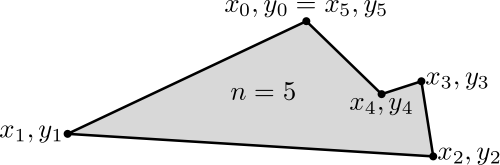
\includegraphics[scale=.5]{images/polygonEx}
\caption{An example polygon for $n=5$}
\label{fig:polygonEx}
\end{figure}

Write a program to open and process a text file containing
$n$ coordinates.  In particular, the first line is a single integer 
$n$ that indicates how many points should be read in.  Each 
line after that has the $x, y$ coordinates of each point separated 
by a single space.

\begin{minted}{text}
4
1.0 0.0
13.2 1.25
20.5 18.4
16.37 24.54
\end{minted}

After reading the file in, it will compute the area of the polygon 
according to the formula above and output it to the user.  For example, 
the output for the above file may be something like \mintinline{text}{Area of the polygon: 197.9135}
\end{exer}

\begin{exer}
Write a program that processes an input text file and scrubs it
of any HTML characters that need to be escaped (see Exercise
\ref{exercise:strings:htmlScrubber} for details).  It should
produce a new output file with all special characters escaped.
\end{exer}

\begin{exer}
Write a program that spell checks a plain text file.  The program
will open a text file and process each word separately, checking 
for proper spelling against a standard dictionary.  

You may assume that each word is separated by some whitespace 
(you may assume that there are no multi-line hyphenated words).  
However, you should ignore all punctuation (periods, question marks, etc.).

Use a standard American dictionary provided on your unix system
which stores words one per line.  Your output should include all
misspelled or unrecognized words (words not contained in the dictionary 
file).
\end{exer}

\begin{exer}
A standard word search consists of an $n \times n$ grid in which there 
are a number of words hidden, some intersecting, with dummy letters 
filling in the blanks.  An example is provided in Figure \ref{fig:wordSearch}.

\begin{figure}[h]
\centering
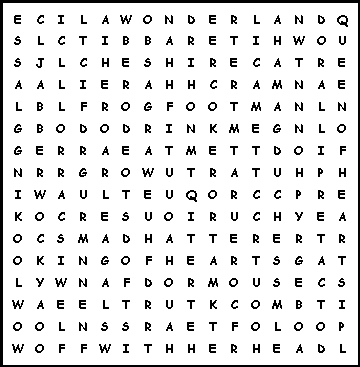
\includegraphics[scale=0.50]{images/wordSearch}
\caption{A Word Search}
\label{fig:wordSearch}
\end{figure}

Write a program to solve a word search.  Your program will read in
an input file with the following format: the first line will contain a 
single integer $n$ which is followed by $n$ lines with $n$ characters 
(not including the end line character) corresponding to the word search.

Once you read in the word search, you will iterate through all possible 
words running down, right, or diagonally down-right.  You will attempt 
to match each possibility against a standard English dictionary.
If the word matches a word in the dictionary, output it to the standard 
output, otherwise ignore it.  To simplify, you may restrict your attention 
to words that have a length between 3 and 8 (inclusive).
\end{exer}

\begin{exer}
Write a crossword puzzle cheater.  The program will take, as input, 
a ``partial'' word in a crossword puzzle.  That is, some of the letters
are known (from other solved clues) while some of the letters are 
not known.  For the purposes of this exercise, we'll use a hyphen 
as a placeholder for missing letters.  

Your program will match the partial word against words in a standard
English dictionary and list all possible matches.  For example, if the 
user provided \mintinline{text}{foo-} as input it might match 
\mintinline{text}{food}, \mintinline{text}{fool}, and \mintinline{text}{foot}.  
\end{exer}

\begin{exer}
Bridge is a four player (2 team) game played with a standard 52-card 
deck.  Prior to play, a round of bidding is performed to determine which 
team is playing for or against the contract, the trump suit, and at what 
level.  Understanding the rules of the game or the bidding conventions 
involved are not necessary for this exercise.  Instead, write a program 
to assist players in how they should bid based on the following point 
system.

A standard 52-card deck is dealt evenly to 4 different hands (Players 
1 thru 4, 13 cards each).  Each player's hand is worth a number of 
points based on the following rules:
\begin{itemize}
  \item Each Ace in the hand is worth 4 points
  \item Each King is worth 3
  \item Each Queen is worth 2
  \item Each Jack is worth 1
  \item For each suit (Diamond, Spade, Club, Heart) such that the hand has only 2 cards (a ``doubleton'') an additional point is added
  \item For each suit that the hand has only 1 card in (a ``singleton'') two additional points are added
  \item For each suit that the hand has no cards (a ``void'') 3 additional points are added.
\end{itemize}
Write a program that reads in a text file containing a deal.  The formatting 
is as follows: the input file will have 4 lines, one for each player.  Each 
line contains the cards dealt to that player delimited by a single space.  
The cards are indicated by the rank ($A, K, Q, J, 10, 9, \ldots, 2$) and 
the suit (D, S, C, H).  An example:

\begin{minted}{text}
3C 3D 7S QD KC AS 6S AC JS 4S JD 7H 6D
5D 8C 7D AH 3H QC 8D JH 5H 9D 7C 9C 4D
2H 10D 8H KS QH 4C 10S 9S 6H 8S KD AD QS
2D 10C 6C 2C 10H 4H 2S 3S 5C 9H KH JC 5S
\end{minted}

Your program should process the file and output the total number 
of points each hand represents.  You should not make any assumptions 
about the ordering of the input.

\begin{minted}{text}
Hand 1 Points: 17
Hand 2 Points: 10
Hand 3 Points: 16
Hand 4 Points: 6
\end{minted}
\end{exer}

\begin{exer}
The game of Sudoku is played on a $9 \times 9$ grid in which
entries consist of the numbers 1 thru 9.  Initially, the board is 
presented with some values filled in and others blank.  The player 
has to fill in the remaining values until all grid boxes are filled and
the following constraints are satisfied.
\begin{itemize}
  \item In each of the 9 rows, each number, 1--9 must appear exactly once
  \item In each of the 9 columns, each number 1--9 must appear exactly once
  \item In each of the $3 \times 3$ sub-grids, each number 1--9 must appear exactly once
\end{itemize}
A full example is presented in Figure \ref{fig:sudoku01}.
\begin{figure}[h]
\centering
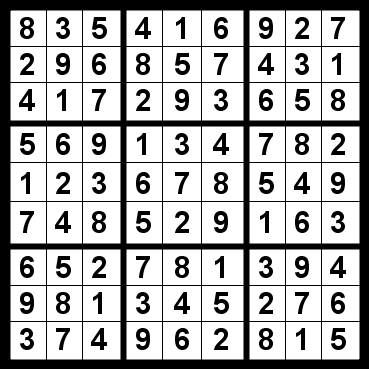
\includegraphics[scale=0.50]{images/sudoku01.png}
\caption{A solved Sudoku puzzle}
\label{fig:sudoku01}
\end{figure}

Write a program that processes a text file containing a possible 
sudoku solution and determine if it is a \emph{valid} or \emph{invalid} 
solution.  The file will have the following format: it will contain 9 lines 
with 9 numbers on each line delimited by a single space.  If the input 
represents a valid solution, output "Valid Solution", otherwise output at 
least one reason why the input is not a valid solution.
\end{exer}

\begin{exer}
Write a program that parses and processes a data file containing 
Comma Separated Values (CSV) and produce an equivalent
JSON (JavaScript Object Notation) output file containing the same 
data.  

The input file will have the following format.  The first line is a CSV 
list of column names.  Each subsequent line is an individual record 
with values for each column. The number of columns and rows may 
vary from file to file.  The following is an example containing data 
about students, which has four columns and 3 records.

\begin{minted}{text}
lastName,firstName,NUID,GPA
Castro,Starlin,11223344,3.48
Rizzo,Anthony,55667788,3.95
Bryant,Chris,01234567,2.7
\end{minted}

The output file will be formatted in JSON where each ``object'' 
(record) is denoted with opening and closing curly brackets, each 
record is separated by a comma, and all records are enclosed in 
square brackets (putting them in an array).  For each record, each 
value is denoted with a key (the column name) and a value.  For
this exercise, treat all values as strings even if they are numbers.  
For example, the input file above would be formatted as follows.

\begin{minted}{json}
[
  {
    "lastName": "Castro",
    "firstName": "Starlin",
    "NUID": "11223344",
    "GPA": "3.48"
  },
  {
    "lastName": "Rizzo",
    "firstName": "Anthony",
    "NUID": "55667788",
    "GPA": "3.95"
  },
  {
    "lastName": "Bryant",
    "firstName": "Chris",
    "NUID": "01234567",
    "GPA": "2.7"
  }
]
\end{minted}

\end{exer}

\begin{exer}
Ranked voting elections are elections where each voter 
\emph{ranks} each candidate rather than just voting for a 
single candidate.  If there are $n$ candidates, then each
voter will rank them 1 (best) through $n$ (worst).  Usually, 
the winner of such an election is determined by a 
\emph{Condorcet} method (the candidate that would
win in by a majority in all head-to-head contests).  
However, we'll use an alternative method, a \emph{Borda count}.

In a Borda count, points are awarded to each candidate 
for each ballot.  For every number 1 ranking, a candidate 
receives $n$ points, for every 2 ranking, a candidate gets 
$n-1$ points, and so on.  For a rank of $n$, the candidate 
only receives 1 point.  The candidates are then ordered by 
their total points and the one with the highest point count 
wins the election.  Such a system usually leads to a 
``consensus'' candidate rather than one preferred by a 
majority.

Implement a Borda-count based ranked voting program.  
Your program will read in a file in the following format.  
The first line will contain an ordered list of candidates 
delimited by commas.  Each line after that will represent 
a single ballot's ranking of the candidates and will contain 
comma delimited integers 1 through $n$.  The order of 
the rankings will correspond to the order of the candidates 
on the first line.

Your program will take an input file name as a command 
line argument, open the file and process it.  It will then 
report the results including the point total for each candidate 
(in order) as well as the overall winner.  It will also report the
total number of ballots.  You may assume each ballot is 
valid and all rankings are provided.

An example input:

\begin{minted}{text}
Alice,Bob,Charlie,Deb
2,1,4,3
3,4,2,1
4,2,3,1
3,2,1,4
3,1,4,2
\end{minted}

An example output:

\begin{minted}{text}
Election Results
Number of ballots: 5

Candidate  Points
Bob        15
Deb   	   14
Charlie    11
Alice      10

Winner is Bob
\end{minted}
\end{exer}

\begin{exer} 
A DNA sequence is a sequence of some combination of the 
characters \mintinline{text}{A} (adenine), \mintinline{text}{C} (cytosine), 
\mintinline{text}{G} (guanine), and \mintinline{text}{T} (thymine) 
which correspond to the four nucleobases that make up DNA.  
Given a long DNA sequence, its often useful to compute the 
frequency of \emph{n-grams}.  An $n$-gram is a DNA subsequence 
of length $n$.  Since there are four bases, there are $4^n$ possible 
$n$-grams.

Write a program that processes a DNA sequence from a plaintext
file and, given $n$, computes the relative frequency of each $n$-gram 
as it appears in the sequence.  As an example, consider the sequence in Figure \ref{figure:dnaSequence}.

\begin{figure}[h]
\centering
\mintinline{text}{GGAAGTAGCAGGCCGCATGCTTGGAGGTAAAGTTCATGGTTCCCTGGCCC}
\caption{A DNA Sequence}
\label{figure:dnaSequence}
\end{figure}

To compute the frequency of all $n=2$ $n$-grams, we would 
consider all 16 combinations of length-two DNA sequences.  We 
would then go through the sequence and count up the number of 
times each $2$-gram appears.  We then compute the relative 
frequency (note: if a sequence is length $L$, then the total number 
of $n$-grams in it is $L - (n - 1)$).  The relative frequency of each 
such $2$-gram is calculated below.

\begin{minted}{text}
AA  6.1224%
AC  0.0000%
AG 10.2041%
AT  4.0816%
CA  6.1224%
CC 10.2041%
CG  2.0408%
CT  4.0816%
GA  4.0816%
GC 10.2041%
GG 12.2449%
GT  8.1633%
TA  4.0816%
TC  4.0816%
TG  8.1633%
TT  6.1224%
\end{minted}
\end{exer}

\begin{exer}
Given a long DNA sequence, it is often useful to compute
the number of instances of a certain \emph{subsequence}.
As an example, if we were to search for the subsequence 
$GTA$ in the DNA sequence in Figure \ref{figure:dnaSequence}, 
it appears twice.  As another example, in the sequence 
\mintinline{text}{CCCC}, the subsequence \mintinline{text}{CC} 
appears three times.

Write a program that processes a text file containing a DNA
sequence and, given a subequence $s$, searches the DNA 
sequence and counts the number of times $s$ appears.
\end{exer}

\begin{exer}
Protein sequencing in an organism consists of a two step 
process.  First the DNA is translated into RNA by replacing 
each thymine (T) nucleotide with uracil (U).  Then, the RNA 
sequence is translated into a protein according to the following 
rules.  The RNA sequence is processed 3 bases at a time.  
Each \emph{trigram} is translated into a single amino acid
according to known encoding rules.  There are 20 such amino 
acids, each represented by a single letter in $(A,C,D,E,F,G,H,I,K,L,M,N,P,Q,R,S,T,V,W,Y)$.

The rules for translating trigrams are presented in Figure 
\ref{figure:codonTable}.  Each triple defines a protein, 
but we're only interested in the first letter of each protein.
Moreover, the trigrams UAA, UAG, and UGA are special 
markers that indicate a (premature) end to the protein 
sequencing (there may be additional nucleotides left in the 
RNA sequence, but they are ignored and the translation 
ends).  

\begin{figure}[h]
\centering
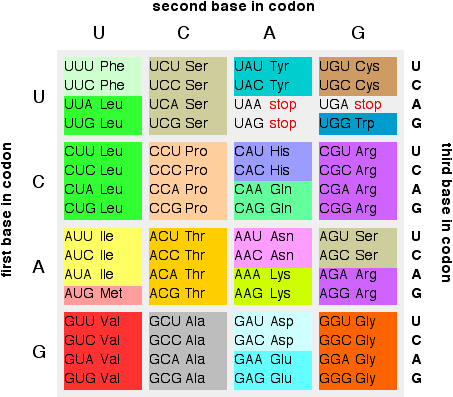
\includegraphics[scale=0.65]{images/codonTable}
\caption{Codon Table for RNA to Protein Translation}
\label{figure:codonTable}
\end{figure}

As an example, suppose we start with the DNA sequence 
$AAATTCCGCGTACCC$; it would be encoded into RNA
as $AAAUUCCGCGUACCC$; and into an amino acid 
sequence $KFRVP$.

Write a program that processes a file containing a DNA
sequence and outputs the translated proteins (only the
first letter of each protein) to an output file.
\end{exer}

\begin{exer}
Recently, researchers have successfully inserted two new 
artificial nucleases into simple bacteria that successfully 
reproduced the artificial bases through several generations.  
The artificial bases d5SICS and dNaM, ($X$ and
$Y$ for short) mimic the natural $G$, and $C$ nucleobases 
respectively.  

Write a program that takes a normal DNA sequence and replace 
some of its $G, C$ pairs with $X, Y$ respectively.  DNA is translated 
into RNA which is then translated into 20 different amino acids.  
Each amino acid produced depends on a 3 nucleobase \emph{codon}.  
For this exercise, we will change $G, C$ pairs with $X, Y$ pairs but
only in codons that represent the amino acids Threonine (an 
essential amino acid) and Alanine (a non-essential amino acid).
Table \ref{table:aminoAcids} contains the codons corresponding 
to these amino acids and the codons you  should translate each one 
to.  All other codons should not be modified.

Your program should open and process a DNA sequence contained in
a file and modify the DNA sequence as described above and output
the artificial DNA sequence to a new output file.  

\begin{table}[h]
\center
\begin{tabular}{|c|c|c|}
\hline
Amino Acid & Codon & Artificial Codon \\
\hline
\hline
\multirow{4}{*}{Threonine} & ACT & AYT \\
~& ACC & AYY \\
~& ACA & AYA \\
~& ACG & AYX\\
\hline
\multirow{4}{*}{Alanine} & GCT & XYT \\
~& GCC & XYY \\
~& GCA & XYA \\
~& GCG & XYX \\
\hline
\end{tabular}
\caption{Amino Acid Codons}
\label{table:aminoAcids}
\end{table}
\end{exer}




%CHAPTER: Encapsulation
\chapter{Encapsulation \& Objects}
\label{chapter:objects}
\index{objects}
%!TEX root = ComputerScienceOne.tex

%%Chapter: Encapsulation

One reason we prefer to write programs in high-level programming
languages is that we can write programs using syntax that is closer 
to plain English.  Granted, programming language syntax is a far cry 
from ``natural'' language, but it is far closer than lower level 
languages such as assembly or binary machine code.  However, from
what we've seen so far, when writing programs we are still forced
to utilize the primitive variable types built-in to the language
we're using.  This is still quite limiting.

As a motivating example, suppose we were to write a program that
involved organizing the enrollment of students into courses.  To
model a particular student, we would need a collection of variables, 
say a first name, last name, GPA, and a unique identification number
(likely a lot more, but let's keep it simple).  Each of these
pieces of data could be modeled by strings, a floating-point number
and perhaps an integer.\footnote{Depending on the identification
number, it may be more appropriately modeled with a string.  Social
Security Numbers for example are not purely numeric: they include
dashes and may begin with zeros.}  Each of these pieces of 
data are stored in separate, unrelated variables even though they
represent a single \emph{entity}.  

Even worse, suppose that we needed to keep track of a collection
of students.  Each piece of data would need to be stored in 
a separate array.  If we wanted to rearrange the data (say, sort
it), we would need to do a lot of manual bookkeeping to make sure
that the separate pieces of data that represented a single entity
were all aligned at the same index in each of the arrays.  If we
wanted to pass the data around to functions, we'd be forced to
pass multiple arrays to each function.  This becomes all the more
complex when we attempt to model entities with more pieces of 
data.  

The solution is to \emph{encapsulate} the pieces of data into
one logical entity, sometimes referred to as an \emph{object}.  
More formally, \emph{encapsulation} is a mechanism by which
pieces of data can be grouped together along with the functions
that operate on that data.  Encapsulation may also provides a 
means to \emph{protect} that data by controlling the visibility
of that data from code outside the object.

Contrast this with an array which is also a collection of data.
However, an array usually contains pieces of similar data while
an object may collect pieces of dissimilar data that make up a
larger entity.  Its kind of like the difference between rows
and columns in a table.  Consider the student data in Table
\ref{table:studentData}.  Each row represents a record while each
column represents a collection of data from each record.  A
single column is comparable to an array while each row is comparable
to an object.  In this example, each object has four pieces of data
encapsulated in it, a first name, last name, an ID, and a GPA.

\begin{table}
\centering
\begin{tabular}{|l|l|l|l|}
\hline
First Name & Last Name & ID & GPA \\
\hline\hline
Tom & Baker & 74 & 3.75 \\
\hline
Christopher & Eccleston & 5 & 3.5 \\
\hline
David & Tennant & 10 & 4.0 \\
\hline
Matt & Smith & 29 & 3.2 \\
\hline
Peter & Capaldi & 13 & 2.9 \\
\hline
\end{tabular}
\caption{Student Data}
\label{table:studentData}
\end{table}

Without objects, to represent this data in code we would need at least
4 separate arrays, more if we wanted to model more data for a student.  
Moreover, data in separate arrays or collections have no real logical
relationship to each other.  The solution that most programming languages
provide is allowing you to \emph{define} an object or structure that
collects pieces of data into one logical unit, allowing you to \emph{name}
the object (say ``Student'') so that you can deal with the data in
a more abstract way.  With objects, we can treat each row in the table
as a single, distinct entity allowing us to collect student objects
into a single array or collection rather than many separate ones.

\section{Objects}

Though languages will differ in how they support objects, they all have
some commonalities.  A language needs to provide ways to define objects,
create \emph{instances} of objects, and to use them in code.

\subsection{Defining}

Most object oriented programming languages such as C++ and Java are 
\emph{class-based} languages.  Meaning that they allow you to define
objects by declaring and defining a ``class.''  A class is essentially
a blue print for what the object \emph{is} and how it is defined.  
Generally, a class declaration allows you to specify member variables
and member methods.  Further, full encapsulation is achieved by using
\emph{visibility} keywords such as \mintinline{java}{public} or
\mintinline{java}{private} to either allow or restrict access to variables
and methods from code \emph{outside} the object.  

Some languages (such as C) do not support full encapsulation, rather they
allow you to define \emph{structures} which allow for the grouping of data, 
but make it difficult or impossible to achieve the other two aspects of
encapsulation (the grouping of methods that act on that data and the
protection of data).

In either case, a language usually allows you to define the member variables
and to \emph{name} the class or structure so that instances can be referred
to by that \emph{type}.  Built-in types such as numbers or strings already
have a type name defined by the language.  However, an object is a 
\emph{user-defined} type that is not built in to the language.  Once defined,
however, the class or structure \emph{can} be referred to just like any
built-in variable type.

Often, it is usual to create objects that are made of other objects.  For
example, a student object may be defined by using two strings for its first
and last name.  In the language, a string itself may be an object.  As a
more complex example, suppose that we wanted an additional member variable
to model a student's date of birth.  A date may itself be an object as it
consists of several pieces of information (a year, month, and date at least).
When an object ``owns'' an instance of another object it is referred to
as \emph{composition} \index{composition} as the object is \emph{composed} of 
other objects.  Further, an object may consist of a \emph{collection}
of other objects (suppose that a student object owned an array of 
course objects representing their schedule).  This is a form of composition
known as \emph{aggregation} (multiple objects have been aggregated
by the object).

\subsection{Creating}

Once a blueprint for an object (or structure) has been declared and defined, 
the second element that a language usually provides for is a way to 
\emph{create} instances of the object.  The concept of an ``object'' is
general and abstract.  Its like the \emph{idea} of a student.  Only once
we have created an actual instance that lives in memory do we have an 
actual \emph{instance}.  Creating instances of an object is usually
referred to as \emph{instantiation}.  

Languages may be able to automatically create instances of your object
with \emph{default} values.  After all, your object is likely 
\emph{composed} of built-in types.  The student example above for
example could be modeled with two strings, an integer, and a floating
point number.  The language/compiler/interpreter ``knows'' how to deal
with these built-in types, so it can extend that knowledge to create
instances of your object which are essentially just collections of 
types that it already knows how to deal with.

Object oriented languages usually provide a special method for you to
be able to give more specifics about how an object is created.  These
are called \emph{constructor} methods.  Sometimes you can define 
multiple constructors methods that take different number(s) of arguments
and/or have different behavior.  Constructor methods typically have
special syntax or have the same name as the class.

In other languages that do not fully support object-oriented programming, 
you must define utility functions that can be used to create instances 
of your object.  Sometimes these are referred to as \emph{factory} functions 
as they are responsible for ``manufacturing'' instances of your object.

\subsection{Using Objects}

After defining and then creating an object, you can usually use it like
any regular variable.  In a strongly typed language you would declare a
variable whose type matches the declared class or structure.  The variable
type can usually be passed and returned from functions, assigned to 
other variables, etc.

A language can also provide a means to access the member variables or
methods that are \emph{visible} to the outside world.  Languages usually
allow you to do this through the ``dot operator'' or the ``arrow operator''.
Suppose we have an instance of a student object stored in a variable
\mintinline{c}{s}.  To access the first name of this instance, we may
be able to use either \mintinline{c}{s.firstName} or 
\mintinline{c}{s->firstName}.  We can access and invoke visible methods 
likewise.  

The dot/arrow operators are how code \emph{outside} the object interacts
with the object.  Outside code is able to do this because it holds a 
reference, \mintinline{c}{s} to the object.  However, \emph{inside} the
object, we may not have a reference (the variable \mintinline{c}{s} was
ostensibly declared and used outside the object and so is not in
scope inside the object).  However, we still have need to reference
member variables or methods from inside the object.  Many languages
provide a means to do this using \gls{open recursion} \index{open recursion}
using a keyword such as \mintinline{java}{this} or \mintinline{php}{self}
or something similar.  The keyword is essentially a self-reference to
the object itself so that you can refer to ``this'' object from within
the object.

\section{Design Principles \& Best Practices}

Using objects in your code follows more of a bottom-up design rather than
a top-down design approach.  In a top-down design, a program is designed
by breaking a program or problem down into smaller and smaller components.
A bottom-up design approaches a problem differently.  First, real-world
entities involved with the problem are modeled by defining objects.  
Then objects are used as building blocks that can be combined and made
to interact to solve a problem.

Object design is usually a straightforward process.  Typically an object
is modeling a real-world entity, so it is simple enough to decompose the
entity into its constituent components.  We do this until the component
can either be modeled by a built-in type such as a string or number or
by an existing object.  In general, you want to keep things as simple
as possible.  Any time you need to associate pieces of data together into
one logical unit, it is likely appropriate to encapsulate them
into an object.

A good design principle is to utilize composition as much as possible.
If you have multiple pieces of data that define a logical entity or 
unit, it is good design to create another object.  For example, if a
student object needs to model a mailing address; think about what an
address is: it is a street address, city, state, zip, etc.  Rather
than having these as member fields to your object, it is probably
more appropriate to define an ``address'' object, especially if such
an object would be useful elsewhere in a program.


%!TEX root = ComputerScienceOne.tex

%Encapsulation - exercises

\section{Exercises}

\begin{exer}
A \emph{complex} number consists of two real numbers: a real
component $a$ and an imaginary component $bi$ where
$i - \sqrt{-1}$.  Define an object or structure to model a
complex number.  Write functions to:
\begin{itemize}
  \item Create a complex number
  \item Print a complex number
  \item Perform basic arithmetic operations on two complex
  	numbers including addition, subtraction and multiplication 
	as defined by:
	$$c_1 + c_2 = (a_1 + b_1i) + (a_2 + b_1i) = (a_1+a_2) + (b_1+b_2)i$$
	$$c_1 - c_2 = (a_1 + b_1i) - (a_2 + b_1i) = (a_1-a_2) + (b_1-b_2)i$$
	$$c_1 \cdot c_2 = (a_1 + b_1i) \cdot (a_2 + b_1i) = 
	  (a_1a_1-b_1b_2) + (a_1b_2+b_1a_1)i$$
\end{itemize}
\end{exer}

\begin{exer}
Design an object (or structure) that models an album.  Include
at least the album title, artist (or band) and release year.
Include any other data that you think is relevant and write
functions to support your object.
\end{exer}



%CHAPTER: Recursion
\chapter{Recursion}
\label{chapter:recursion}
\index{recursion}
%!TEX root = ComputerScienceOne.tex

%%Chapter: Recursion

Suppose we wanted to write a simple program that performed a 
countdown, printing
10, 9, 8, \ldots, 2, 1 and when it reached zero it printed a ``Happy
New Year'' message.  Likely our first instinct would be to write a 
very simple for loop using an increment variable.  But suppose
we lived in a world \emph{without} the usual loop control structures 
that we are now
familiar with.  How might we write such a program?

After thinking about it for a while, we might think: well, we don't have
loops, but we still have functions.  In particular what if we had a function
that took the ``current'' value of our counter variable and decremented it, 
passing it to another function, which did the same thing.  For example, we 
could pass 10 to such a function, which would then subtract 1, passing 9
to another function and so on.  A check could be made to see if the value was 
zero, in which case we print our special message and no longer call any more 
functions.

In fact, we would not need to define 10 different functions to do so.  Instead, 
we could define one function that \emph{called itself}.  It might look something
like Algorithm \ref{algo:recursiveCountdown}.

\begin{algorithm}[H]
  \Input{An integer $n \geq 0$}
  \Output{A countdown of integers $n, \ldots 0$}
 
  \eIf{$n = 0$}{
    output ``Happy New Year!!!'' \;
  }{
    output $n$ \;
    $\textsc{CountDown}(n-1)$ \label{algo:line:recursiveCall} \;
  }
\caption{Recursive $\textsc{CountDown}(n)$ Function}
\label{algo:recursiveCountdown}
\end{algorithm}

The function in this case is called $\textsc{CountDown}()$.  In Line 
\ref{algo:line:recursiveCall} the function calls itself on a decremented
value.  When a function calls itself, it is a \emph{recursive} function.
When a allows functions to call themselves they support \emph{recursion}.

This is not that odd of a concept.  We've seen many examples where functions
invoke other functions.  Each function call simply creates
a new stack frame on the program stack.  There is nothing particularly special
about which functions call which other functions, so there is little
difference when a function calls itself. 

This was not just a toy example.  There are many programming languages in which
recursion is used as a matter of course.  Functional programming languages
tend to avoid control structures like loops and even (mutable) variables.  
Instead, control flow is defined by evaluating a series of functions, making
recursion a fundamental technique.

Recursion is extensively used in mathematics.  Recurrence relations or
recursive functions are common.  The Fibonacci sequence is
a common, if not overused\footnote{The Fibonacci sequence is nothing
special; its simply a second order linear homogenous recurrence relation
with coefficients of 1.  The 
near reverence that so many people attribute to it borders on mysticism.}
example.  It has a simple definition: the next value in the sequence is
simply the sum of the two previous values.  The sequence starts with the 
\emph{initial values} of 1.  The first few terms in the sequence:
  $$1, 1, 2, 3, 5, 8, 13, 21, 34, 55, 89, \ldots$$
The more formal mathematical definition can be stated as follows.
\[
F_n = \left\{
\begin{array}{ll}
1 & \text{if } n = 0 \\
1 & \text{if } n = 1 \\
F_{n-1} + F_{n-2} & \text{otherwise}
\end{array}
\right.
\]

The Fibonacci sequence is the cliche example for recursion.  We can 
define an algorithmic function to compute the $n$-th Fibonacci number
as follows.

\begin{algorithm}[H]
  \Input{An integer $n \geq 0$}
  \Output{The $n$-th Fibonacci number, $F_n$}
 
  \eIf{$n \leq 1$}{
    output 1 \;
  }{
    output $\textsc{Fibonacci}(n-1) + \textsc{Fibonacci}(n-2)$ \;
  }
\caption{Recursive $\textsc{Fibonacci}(n)$ Function}
\label{algo:recursiveFibonacci}
\end{algorithm}

Though hackneyed, it does provide a good example for how recursive functions
work.  We'll also utilize it as an example of \emph{why you should avoid
recursion in practice}.  We use it to illustrate how the problems
with recursion can be mitigated or avoided altogether.

\section{Writing Recursive Functions}

When writing a recursive function, there are several key elements that
we need to take care of to ensure that it executes correctly.  In particular, 
every recursive function requires at least one \emph{base case} or
base condition which serves as a terminating condition for the recursion.
A base case is a condition which, instead of making a recursive call, 
processes and returns a value.  Without a base case, the recursion would 
continue unbounded: the  function would call itself over and over again, 
creating new stack frame after stack frame until we run out of stack space.  
If a program makes too many function calls and runs out of stack memory, 
it may lead to a \gls{stack overflow} and the 
termination of the program.  Even if we don't have
unbounded recursion, it is still possible to run out of stack space
even with simple recursion.

The other key element that we need is to ensure that every recursive
call \emph{makes progress} toward one of the terminating conditions.  
If no progress is made, then again we may have an unbounded recursion.
In the Fibonacci example in Algorithm \ref{algo:recursiveFibonacci}, the
base case can be found in the first if-statement: when $n$ reaches $1$
or less, no recursive calls are made.  In the else-statement, we make
two recursive calls, but both of them make progress toward this base 
case.  The first decrements $n$ by 1 and the second by 2, eventually
reaching $n = 1$.

\subsection{Tail Recursion}
\index{tail recursion}

Making many function calls can be costly in terms of stack space.  One
optimization that can be made is to use \emph{tail recursion}.  The last
operation that a function executes is referred to as the \emph{tail}
operation.  If a function invokes another function as its tail operation, 
its a \emph{tail call}.  For example, consider the following snippet of
code:

\begin{minted}{c}
int foo(int x) {
  ...
  return bar(x-1) + 1;
}
\end{minted}

Here, \mintinline{c}{foo()} calls \mintinline{c}{bar()} but it is 
\emph{not} the last operation before it returns.  Instead, it invokes
\mintinline{c}{bar()}, takes the result and adds one \emph{then} 
returns to the calling function.  Note that decrementing \mintinline{c}{x}
is performed \emph{before} the invocation of \mintinline{c}{bar()}.
In contrast, consider the following modified code:

\begin{minted}{c}
int foo(int x) {
  ...
  return bar(x-1);
}
\end{minted}

Here, the invocation of \mintinline{c}{bar()} is the last operation
performed by \mintinline{c}{foo()}.  Thus, this is a tail call.

Tail calls have the advantage that a language or compiler can generally
optimize the function call with respect to the stack frame.  Since the
function \mintinline{c}{foo()} is essentially done with its computation, 
its stack frame is no longer needed.  The system, therefore, can reuse
the stack frame.  Tail recursion is such an important optimization, some
languages require it or ``guarantee'' it in other ways.

\section{Avoiding Recursion}

Recursion is not essential; some languages do not even support recursion.
In fact, any recursive function can be rewritten to not use recursion.
Usually, you can write an equivalent loop structure or use an in-memory
\gls{stack} data structure to replace the recursion.
So why use it?  Proponents would argue that recursion allows you to 
write simple code that more closely matches mathematical functions and
expressions.  Recursion is also a natural way to think about certain
problem solving techniques such as divide-and-conquer (see Chapter 
\ref{chapter:searchingSorting}).  It is also a natural way to code
in functional programming languages.

These arguments, however, are \emph{subjective}.  One person's 
``cleaner'' or ``more understandable'' code is another person's 
spaghetti code hack.  What is ``natural'' for one person may be 
``weird'' and ``odd'' for another.  However, there are many other
arguments against recursion, many of which are \emph{objective} 
reasons: that recursion is more expensive and can
easily lead to inefficient, exponential algorithms.

In general, recursion requires lots of function calls which requires 
creating and removing lots of stack frames.  This usually results in 
a lot of overhead and resources being used to perform the computation.  
Unless you are using a language in which recursion is optimized and
made to be more efficient (such as functional programming
languages), this is a lot more expensive than using simple loops and
iteration.  

Another reason to avoid recursion is that it can lead to a lot of
extraneous re-computations.  The cliched example of the Fibonacci
recursion is a prime example of this.\footnote{Its overuse as
an example of recursion is even less explicable as it solves a problem
that no one cares about.}  Consider the computation of 
$\textsc{Fibonacci}(5)$.  This results in two recursive calls, each of
those calls results in 2 recursive calls and so on as depicted in 
Figure \ref{figure:fibonacciTree}.

\begin{figure}
\centering

\begin{tikzpicture}
  [scale=.50,transform shape,
   level distance=4cm,
   every node/.style={rectangle,
                      thin,
                      draw=black,
                      %top color = white,
                      %bottom color = black!50,
                      inner sep=5pt,
                      %drop shadow={opacity=0.35,shadow xshift=.2ex, shadow yshift=-.2ex}
                      },
   edge from parent/.style={->,draw,>=latex'},
   level 1/.style={sibling distance=16cm},
   level 2/.style={sibling distance=8cm},
   level 3/.style={sibling distance=4cm},
   level 4/.style={sibling distance=4cm}]
  \node {\mintinline{text}{fibonacci(5)}}
     child {node {\mintinline{text}{fibonacci(4)}}
       child {node {\mintinline{text}{fibonacci(3)}}
         child {node {\mintinline{text}{fibonacci(2)}}
          child {node {\mintinline{text}{fibonacci(1)}}}
          child {node {\mintinline{text}{fibonacci(0)}}}
         }
         child {node {\mintinline{text}{fibonacci(1)}}}
       }
       child {node {\mintinline{text}{fibonacci(2)}}
          child {node {\mintinline{text}{fibonacci(1)}}}
          child {node {\mintinline{text}{fibonacci(0)}}}
       }
     }
     child {node {\mintinline{text}{fibonacci(3)}}
        child {node {\mintinline{text}{fibonacci(2)}}
          child {node {\mintinline{text}{fibonacci(1)}}}
          child {node {\mintinline{text}{fibonacci(0)}}}
        }
        child {node {\mintinline{text}{fibonacci(1)}}}
     };
\end{tikzpicture}

\caption{Recursive Fibonacci Computation Tree}
\label{figure:fibonacciTree}
\end{figure}

As depicted in the figure, several function calls are repeated: 
$\textsc{Fibonacci}(3)$ is called twice, $\textsc{Fibonacci}(2)$
is called 3 times, etc.  15 total function calls are made to
compute $\textsc{Fibonacci}(5)$.  In general, the computation
of $\textsc{Fibonacci}(n)$ will result in an \emph{exponential}
number of function calls.  The number of function calls
to compute $F_n$ with this recursive solution will be equal to 
  $$F_{n-2} + \sum_{i=0}^{n-1} F_{i}$$ 
That is more than the first $n-1$ Fibonacci numbers combined!
It should come as no surprise that the Fibonacci sequence
grows \emph{exponentially} and thus so would the number of 
operations with this recursive solution.

To put this in perspective, consider computing $F_{45} = 1,836,311,903$ 
($n = 45)$, the maximum representable value for a 32-bit signed two's
complement integer.  Executing a C implementation of this recursive
algorithm took about 8 seconds\footnote{On a 2.7GHz Intel Core i7.} 
and required 3,672,623,805 function calls!

What if we wanted to compute $F_{100} = 573,147,844,013,817,084,101$ 
(573 quintillion) it would result in 1,146,295,688,027,634,168,201 
(1.146 sextillion) function calls.  Using the same hardware, at 
$4.59\times 10^8$ (459 million) function calls per second, it would
take $2.497 \times 10^{12}$ seconds to compute.  That would be more than
79,191 \emph{years}!  Even if we performed these (useless) calculations
on hardware that was 1 million times faster than my laptop, it would
still take over 4 \emph{weeks}!

\subsection{Memoization}
\index{memoization}

The inefficiency in the example above comes from the fact that we make 
the same function calls on the same values over and over.  One way to
avoid recomputing the same values is to \emph{store} them into a table
(or \emph{tableau} if you prefer being fancy).  Then, when you need
to compute a value, you look at the table to see if it has already
been computed.  If it has, we reuse the value stored in the table, otherwise
we compute it by making the appropriate recursive calls.  Once computed,
we place the value into the table so that it can be looked up on subsequent
function calls.  This approach is usually referred to as \gls{memoization}.

The ``table'' in this scenario is very general: it can be achieved using 
a number of different data structures including simple arrays, or even
maps (mapping input value(s) to output values).  The table is essentially
serving as a \index{cache} \gls{cache} for the previously computed values. An 
illustration of how this might work can be found in Algorithm 
\ref{algo:recursiveFibonacciMemoization}.  Here, the recursion only
occurs if the value $F_n$ is not yet defined.

\begin{algorithm}[H]
  \Input{An integer $n \geq 0$, a global map $M$ that maps $n$ values to $F_n$}
  \Output{The $n$-th Fibonacci number, $F_n$}
 
  \eIf{$F_n$ is defined in $M$}{
    output $M(n)$ \;
  }{
    $a \leftarrow \textsc{Fibonacci}(n-1)$ \;
    $b \leftarrow \textsc{Fibonacci}(n-2)$ \;
    Define $M(n) = a + b$ \;
    output $(a + b)$ \;
  }
\caption{Recursive $\textsc{Fibonacci}(n)$ Function With Memoization}
\label{algo:recursiveFibonacciMemoization}
\end{algorithm}

In many functional programming languages, memoization is implicit and
provided by the language itself to ensure that we do not have the same
problems with recomputing values as we observed above.  In languages
such as C and Java, memoization becomes our responsibility and is not
an optimization provided by the language itself.  

However, if we are filling in a table of values anyway, we
really don't need to make recursive calls at all.  We simply need to 
figure out in what order to fill out the values in the table.  This is
actually the basis of a powerful programming technique known as
\index{dynamic programming} \gls{dynamic programming} which is a 
``bottom-up'' approach to solving problems by combining solutions 
to smaller ones.



%!TEX root = ComputerScienceOne.tex

%Recursion - exercises

\section{Exercises}

\begin{exer}
The binomial coefficients, $C(n,k)$ or ${n \choose k}$ (``$n$ choose
$k$''), are defined as the number of ways you can select $k$ distinct
items from a collection of $n$ items.  A direct combinatorial
definition is
$${n \choose k} = \frac{n!}{k!(n-k)!}$$
An alternative is Pascal's identity, which gives a recurrence to
compute this value:
$${n \choose k} = {n-1 \choose k} + {n-1 \choose k-1}$$
Where ${n \choose 0} = 1$ for any $n$ and for all $k > n$, ${n\choose
k} = 0$. Finally, ${n \choose 1} = n$.
\begin{enumerate}
  \item Write a recursive function using Pascal's identity to compute
  	${n \choose k}$.  Benchmark its performance.
  \item Write a recursive version that uses memoization to avoid 
  	recomputing values
  \item Modify your functions to utilize an arbitrary precision 
  	numeric type so that you can compute arbitrarily large values.
\end{enumerate}
\end{exer}

\begin{exer}
The Jacobsthal sequence is very similar to the Fibonacci sequence 
in that it is defined by its two previous terms.  The difference is that 
the second term is multiplied by two.  
$$J_n = \left\{
\begin{array}{ll}
0 & \textrm{if } n = 0 \\
1 & \textrm{if } n = 1 \\
J_{n-1} + 2J_{n-2} & \textrm{otherwise}
\end{array}
\right.$$

\begin{enumerate}
  \item Write a recursive function that computes the $n$-th Jacobsthal
    number.  Benchmark its performance.
  \item Write a recursive version that uses memoization to avoid 
  	recomputing values
  \item Modify your functions to utilize an arbitrary precision 
  	numeric type so that you can compute arbitrarily large values.
\end{enumerate}
\end{exer}



%CHAPTER: Searching & Sorting
\chapter{Searching \& Sorting}
\label{chapter:searchingSorting}
\index{searching}
\index{sorting}
%!TEX root = ComputerScienceOne.tex

%%Chapter: Searching & Sorting

Searching and sorting are two fundamental operations when dealing
with collections of data.  Both operations are not only important in
and of themselves, but they also form the basis of many algorithms
and other more complex operations.  These operations are so essential 
that a wide variety
of algorithms and techniques have been developed to solve them, each
with their own advantages and disadvantages.  This variety provides
a good framework from which to study the relative efficiency and complexity
of algorithms through algorithm analysis.

\section{Searching}
\index{searching}

Searching is a very basic operation.  Given a collection of data, we
wish to find a particular element or elements that match a certain 
criteria.  More formally, we have the following.

\begin{problem}[Searching]
\label{problem:searching}
~\\
\textbf{Given:} a collection of elements, $A =\{a_1, a_2, \ldots, a_n\}$ 
and a \emph{key} element $e_k$\\
\textbf{Output:} The element $a_i$ in $A$ such that $a_i = e_k$
\end{problem}

The ``equality'' in this problem statement is not explicitly 
specified.  In 
fact, this is a very general, abstract statement of the basic search 
problem.  We didn't specify that the ``collection'' was an array, a list, 
a set, or any other particular data structure.  Nor did we specify what
type of elements were in the collection.  They could be numbers, they
could be strings, they could be objects.  

There are many variations of this general search problem that we could
consider.  For example, we could generalize it to find the ``first''
or ``last'' such element if our collection is ordered.  We could find
\emph{all} elements that match our criteria.  Some basic operations that 
we've already considered such as finding the minimum or maximum
(\emph{extremal} elements), or median element are also variations on this search 
problem.

When designing a solution to any of these variations additional 
considerations must be made.  We may wish our search to be index-based 
(that is, output the index $i$ rather than the element $a_i$).  We
may need to think about how to handle \emph{unsuccessful} searches 
(return \mintinline{text}{null}?  A special flag value?  Throw an
exception?, etc.).

When implementing a solution in a programming language, we of course
will need to be more specific about the type of collection being
searched and the type of elements in the collection.  However, we
will still want to keep our solution as general as possible.  As we'll 
see, most programming languages facilitate some sort of 
\index{generic programming} \emph{generic}
programming so that we do not need to reimplement the solution for
\emph{each} type of collection or for \emph{each} type of variable.  
Instead, we can write one solution, then \emph{configure} it to allow
for comparisons of any type of variable (numeric, string, object, etc.).

\subsection{Linear Search}
\index{search!linear search}
\index{linear search}

The first solution that we'll look at is the \emph{linear search}
algorithm (also known as sequential search).  This is a basic, 
straightforward solution to the search problem that works by simply
iterating through each element $a_i$, testing for equality, and
outputting the first element that matches the criteria.  The
pseudocode is presented as Algorithm \ref{algo:linearSearch}.

\begin{algorithm}[H]
  \Input{A collection of elements $A = \{a_1, \ldots, a_n\}$ and a key $e_k$}
  \Output{An element $a$ in $A$ such that $a = e_k$ according to some criteria; $\phi$ if no such element exists}
  \ForEach{$a_i \textrm{in the collection} A$}{
    \If{$a_i = e_k$}{ \label{algo:linearSearch:elemOp}
      output $a_i$ \;
    }
  }
  output $\phi$ \;
\caption{Linear Search}
\label{algo:linearSearch}
\end{algorithm}

To illustrate, consider the following example searches.  Suppose we wish
to search the 0-indexed array of integers in Figure \ref{figure:arrayForSearching}.

%\documentclass[12pt]{scrbook}
%
%\usepackage{tikz}
%\usepackage{minted}
%\usetikzlibrary{decorations.pathreplacing,arrows}
%
%\usepackage{fullpage}
%\usepackage{subfigure}
%\begin{document}
%
%
%Lorem Ipsum is simply dummy text of the printing and typesetting industry. Lorem Ipsum has been the industry's standard dummy text ever since the 1500s, when an unknown printer took a galley of type and scrambled it to make a type specimen book. It has survived not only five centuries, but also the leap into electronic typesetting, remaining essentially unchanged. It was popularised in the 1960s with the release of Letraset sheets containing Lorem Ipsum passages, and more recently with desktop publishing software like Aldus PageMaker including versions of Lorem Ipsum.

\begin{figure}
\centering

\begin{tikzpicture}
% size of each node
\def\sz{9mm}
% node style definition
\tikzstyle{block} = [
	draw, fill=black!10, rectangle,
	minimum height=\sz, minimum width=\sz ];
\tikzstyle{plain} = [draw=none,fill=none];
% array element definition
\def\arr{42, 4, 9, 4, 102, 34, 12, 2, 0 };
%\def\x{0}; % x pos of arr
%\def\y{0}; % y pos of arr
%\newcounter{ind};
\setcounter{ind}{0};
\node[plain] at (-1.75, 1) { index };
\node[plain] at (-1.75, 0) { contents };
\foreach \item in \arr
{
	\node[block] at (\theind*\sz,0) { \item };
	\node[plain] at (\theind*\sz,1.0) { \theind };
	\addtocounter{ind}{1};
}
\end{tikzpicture}

\caption[Array of Integers]{Array of Integers}
\label{figure:arrayForSearching}
\end{figure}

%\end{document}



A search for the key $e_k = 102$ would start at the first element.  
$42 \neq 102$ so the search would continue; it would compare it against
4, then 9, then 5, and finally find 102 at index $i = 4$, making a
total of 5 comparisons (including the final comparison to the matched
element).  

A search for the key $e_k = 42$ would get lucky.  It would find it
after only one comparison as the first element is a match.  A search
for the element 20 would result in an unsuccessful search with a 
total of 10 comparisons being made.  Finally a search for $e_k = 4$
would only require two comparisons as we find 4 at the second index.
There is a duplicate element at index 3, but the way we've defined
linear search is to find the ``first'' such element.  Again, we could
design any number of variations on this solution. We give a more 
detailed analysis of this algorithm below.

\subsection{Binary Search}
\index{search!binary search}
\index{binary search}

An alternative search algorithm is \emph{binary search}.  This is a 
clever algorithm that requires that the array being searched is 
\emph{sorted} in ascending order.  Though it works on any type of
data, let's again use an integer array as an example.  Suppose
we're searching for the key element $e_k$.  We start by looking
at the element in the \emph{middle} of the array, call it $m$.

\begin{figure}
\centering
%\documentclass[12pt]{scrbook}
%
%\usepackage{tikz}
%\usepackage{minted}
%\usetikzlibrary{decorations.pathreplacing,arrows}
%
%\usepackage{fullpage}
%\usepackage{subfigure}
%\begin{document}
%
%
%Lorem Ipsum is simply dummy text of the printing and typesetting industry. Lorem Ipsum has been the industry's standard dummy text ever since the 1500s, when an unknown printer took a galley of type and scrambled it to make a type specimen book. It has survived not only five centuries, but also the leap into electronic typesetting, remaining essentially unchanged. It was popularised in the 1960s with the release of Letraset sheets containing Lorem Ipsum passages, and more recently with desktop publishing software like Aldus PageMaker including versions of Lorem Ipsum.
%
%\begin{figure}
%\centering

\begin{tikzpicture}[scale=1.2]

\draw (0,0) rectangle (1,1);
\node (a) at (0.5, 0.5) {$a_1$};

\draw (1,0) rectangle (4,1);
\node at (2.5, 0.5) {$\cdots$};

\draw (4,0) rectangle (5,1);
\node (b) at (4.5, 0.5) {$a_{\frac{n}{2}-1}$};

\draw (5,0) rectangle (6,1);
\node (am) at (5.5, 0.5) {$a_{\frac{n}{2}}$};

\draw (6,0) rectangle (7,1);
\node (c) at (6.5, 0.5) {$a_{\frac{n}{2}+1}$};

\draw (7,0) rectangle (10,1);
\node at (8.5, 0.5) {$\cdots$};

\draw (10,0) rectangle (11,1);
\node (d) at (10.5, 0.5) {$a_{n}$};


\node (m) at (5.5, -0.85) {$m$};
\draw[->,shorten >=0.5cm] (m) -- (am);


  \draw [decorate,decoration={brace,mirror,amplitude=10pt},xshift=-4pt,yshift=0pt] ([xshift=0cm,yshift=-.5cm]a.south) -- ([xshift=0cm,yshift=-0.5cm]b.south) node [black,midway,yshift=-0.75cm] {$< m$};

  \draw [decorate,decoration={brace,mirror,amplitude=10pt},xshift=-4pt,yshift=0pt] ([xshift=0cm,yshift=-.5cm]c.south) -- ([xshift=0cm,yshift=-0.5cm]d.south) node [black,midway,yshift=-0.75cm] {$> m$};


\end{tikzpicture}

%\caption[Array of Integers]{Array of Integers}
%\label{figure:arrayForSearching}
%\end{figure}
%
%\end{document}
%

\caption[A Sorted Array]{When an array is sorted, all elements in the left half are less than the middle element $m$, all elements in the
right half are greater than $m$.}
\label{figure:binarySearchDemo}
\end{figure}

Since the array is sorted, everything in the left-half 
of the array is $< m$ and everything in the right-half of the array 
is $> m$.\footnote{If duplicate elements
are in the array, then elements in the left/right half \emph{could}
be less than or equal to and greater than or equal to $m$, but this
will not affect how our algorithm works.}  We will now make one 
comparison between $e_k$ and $m$. There are three cases to consider.
\begin{enumerate}
  \item If $e_k = m$, then we've found \emph{an} element that matches
  	our key and search criteria and we are done.  We can output
	$m$ and stop the algorithm.
  \item If $e_k < m$ then we know that if a matching element exists, 
  	it must lie in the left-half of the list.  This is because all 
	elements in the right-half are $> m$.
  \item If $e_k > m$ then we know that if a matching element exists, 
  	it must lie in the right-half of the list.  This is because all 
	elements in the left-half are $< m$.
\end{enumerate}

In either of the second two cases, we have essentially cut the array
in half, halving the number of elements we need to consider.  Suppose
that the second case applies.  Then we can consider elements indexed
from $1$ to $\frac{n}{2}-1$ (we need not consider $a_{\frac{n}{2}}$ 
as the first case would have applied if we found a match).  We
can then do the same trick: check the middle element among the 
remaining elements and determine which half to cutout and which
half to consider.  We repeat this process until we've either found
the element we are looking for or the range in which we are searching
becomes ``empty'' indicating an unsuccessful search.

This description suggests a recursive solution.  Given two indices
$l, r$, we can compute the index of the middle element, $m = \frac{l + r}{2}$
and make one of two recursive calls depending on the cases identified
above.  Of course, we will need to make sure that our base case is taken
care of: if the two indices are \emph{invalid}, that is if the left
is greater than the right, $l > r$, then we know that the search
was unsuccessful.

\begin{algorithm}[H]
  \Input{A \emph{sorted} collection of elements $A = \{a_1, \ldots, a_n\}$, 
         bounds $1 \leq l, r \leq n$, and a key $e_k$}
  \Output{An element $a$ in $A$ such that $a = e_k$ according to some criteria; 
          $\phi$ if no such element exists}
  \If{$l > r$}{
    output $\phi$ \;
  }
  $m \leftarrow \lfloor \frac{l + r}{2} \rfloor$ \;
  \uIf{$a_m = e_k$}{ 
    output $a_m$ \;
  }
  \uElseIf{$a_m < e_k$}{ 
    \textsc{BinarySearch}$(A, m+1, r, e_k)$ \;
  }
  \Else{
    \textsc{BinarySearch}$(A, l, m-1, e_k)$ \;
  }
\caption{Recursive Binary Search Algorithm, $\textsc{BinarySearch}(A, l, r, e_k)$}
\label{algo:binarySearchRecursive}
\end{algorithm}

As discussed in Chapter \ref{chapter:recursion}, non-recursive solutions
are generally better than recursive ones.  We can design a straightforward
iterative version of binary search using a while loop.  We initialize two
index variables, $l, r$ and update them on each iteration depending on the
three cases above.  The loop stops when we've found our element or $l > r$
resulting in an unsuccessful search.  The iterative version is presented
in Algorithm \ref{algo:binarySearchIterative}, an example run of the
algorithm is shown in Figure \ref{figure:binarySearchExample}.

\begin{algorithm}[H]
  \Input{A \emph{sorted} collection of elements $A = \{a_1, \ldots, a_n\}$ 
         and a key $e_k$}
  \Output{An element $a \in A$ such that $a = e_k$ according to some criteria; 
          $\phi$ if no such element exists}
  $l \leftarrow 1$ \;
  $r \leftarrow n$ \;
  \While{$l \leq r$}{
    $m \leftarrow \lfloor \frac{l + r}{2} \rfloor$ \;
    \uIf{$a_m = e_k$}{ \label{algo:binarySearch:elemOp1}
      output $a_m$ \;
    }
    \uElseIf{$a_m < e_k$}{ \label{algo:binarySearch:elemOp2}
      $l \leftarrow (m+1)$ \;
    }
    \Else{
      $r \leftarrow (m-1)$ \;
    }
  }
  output $\phi$ \;
\caption{Iterative Binary Search Algorithm, $\textsc{BinarySearch}(A, e_k)$}
\label{algo:binarySearchIterative}
\end{algorithm}

%\documentclass[12pt]{scrbook}
%
%\usepackage{tikz}
%\usepackage{minted}
%\usetikzlibrary{decorations.pathreplacing}
%
%\usetikzlibrary{patterns}
%
%\usepackage{fullpage}
%\usepackage{subfigure}
%\begin{document}
%
%
%Lorem Ipsum is simply dummy text of the printing and typesetting industry. Lorem Ipsum has been the industry's standard dummy text ever since the 1500s, when an unknown printer took a galley of type and scrambled it to make a type specimen book. It has survived not only five centuries, but also the leap into electronic typesetting, remaining essentially unchanged. It was popularised in the 1960s with the release of Letraset sheets containing Lorem Ipsum passages, and more recently with desktop publishing software like Aldus PageMaker including versions of Lorem Ipsum.
%

\begin{figure}
\centering

\subfigure[Initially, $l = 0, r = 10$ and so we examine the middle
element at index $m = 5$ which is 12.]{

\begin{tikzpicture}
% size of each node
\def\sz{9mm}
% node style definition
\tikzstyle{block} = [
	draw, fill=black!10, rectangle,
	minimum height=\sz, minimum width=\sz ];
\tikzstyle{plain} = [draw=none,fill=none];
% array element definition
\def\arr{0, 2, 4, 4, 9, 12, 34, 42, 102};
%\def\x{0}; % x pos of arr
%\def\y{0}; % y pos of arr
%\newcounter{ind};
%\setcounter{ind}{0};
\node[plain] at (-1.75, 1) { index };
\node[plain] at (-1.75, 0) { contents };

\node[block] at (0,0) { -3 };
\node[plain] at (0,1.0) { 0 };

\node[block] at (1*\sz,0) { 2 };
\node[plain] at (1*\sz,1.0) { 1 };

\node[block] at (2*\sz,0) { 4 };
\node[plain] at (2*\sz,1.0) { 2 };

\node[block] at (3*\sz,0) { 4 };
\node[plain] at (3*\sz,1.0) { 3 };

\node[block] at (4*\sz,0) { 9 };
\node[plain] at (4*\sz,1.0) { 4 };

\node[block,fill=white!10!green] at (5*\sz,0) { 12 };
\node[plain] at (5*\sz,1.0) { 5 };

\node[block] at (6*\sz,0) { 34 };
\node[plain] at (6*\sz,1.0) { 6 };

\node[block] at (7*\sz,0) { 42 };
\node[plain] at (7*\sz,1.0) { 7 };

\node[block] at (8*\sz,0) { 102 };
\node[plain] at (8*\sz,1.0) { 8 };

\node[block] at (9*\sz,0) { 157 };
\node[plain] at (9*\sz,1.0) { 9 };

\node[block] at (10*\sz,0) { 180 };
\node[plain] at (10*\sz,1.0) { 10 };


%\foreach \item in \arr
%{
%	\node[block] (a\theind) at (\theind*\sz,0) { \item };
%	\node[plain] at (\theind*\sz,1.0) { \theind };
%	\addtocounter{ind}{1};
%}
\end{tikzpicture}

}

\subfigure[Since $64 > 12$, we update our left index variable
$l$ to $m + 1$, thus $l = 6$ and we've eliminated the left half
of the list from consideration.]{

\begin{tikzpicture}
% size of each node
\def\sz{9mm}
% node style definition
\tikzstyle{block} = [
	draw, fill=black!10, rectangle,
	minimum height=\sz, minimum width=\sz ];
\tikzstyle{plain} = [draw=none,fill=none];
% array element definition
\def\arr{0, 2, 4, 4, 9, 12, 34, 42, 102};
%\def\x{0}; % x pos of arr
%\def\y{0}; % y pos of arr
%\newcounter{ind};
%\setcounter{ind}{0};
\node[plain] at (-1.75, 1) { index };
\node[plain] at (-1.75, 0) { contents };

\node[block,pattern=north west lines, pattern color=blue] at (0,0) { -3 };
\node[plain] at (0,1.0) { 0 };

\node[block,pattern=north west lines, pattern color=blue] at (1*\sz,0) { 2 };
\node[plain] at (1*\sz,1.0) { 1 };

\node[block,pattern=north west lines, pattern color=blue] at (2*\sz,0) { 4 };
\node[plain] at (2*\sz,1.0) { 2 };

\node[block,pattern=north west lines, pattern color=blue] at (3*\sz,0) { 4 };
\node[plain] at (3*\sz,1.0) { 3 };

\node[block,pattern=north west lines, pattern color=blue] at (4*\sz,0) { 9 };
\node[plain] at (4*\sz,1.0) { 4 };

\node[block,fill=white!10!green] at (5*\sz,0) { 12 };
\node[plain] at (5*\sz,1.0) { 5 };

\node[block] at (6*\sz,0) { 34 };
\node[plain] at (6*\sz,1.0) { 6 };

\node[block] at (7*\sz,0) { 42 };
\node[plain] at (7*\sz,1.0) { 7 };

\node[block] at (8*\sz,0) { 102 };
\node[plain] at (8*\sz,1.0) { 8 };

\node[block] at (9*\sz,0) { 157 };
\node[plain] at (9*\sz,1.0) { 9 };

\node[block] at (10*\sz,0) { 180 };
\node[plain] at (10*\sz,1.0) { 10 };




%\foreach \item in \arr
%{
%	\node[block] (a\theind) at (\theind*\sz,0) { \item };
%	\node[plain] at (\theind*\sz,1.0) { \theind };
%	\addtocounter{ind}{1};
%}
\end{tikzpicture}

}



\subfigure[Our new middle index is $m = \frac{l+r}{2} = \frac{6+10}{2} = 8$, 
corresponding to the element 102.]{

\begin{tikzpicture}
% size of each node
\def\sz{9mm}
% node style definition
\tikzstyle{block} = [
	draw, fill=black!10, rectangle,
	minimum height=\sz, minimum width=\sz ];
\tikzstyle{plain} = [draw=none,fill=none];
% array element definition
\def\arr{0, 2, 4, 4, 9, 12, 34, 42, 102};
%\def\x{0}; % x pos of arr
%\def\y{0}; % y pos of arr
%\newcounter{ind};
%\setcounter{ind}{0};
\node[plain] at (-1.75, 1) { index };
\node[plain] at (-1.75, 0) { contents };

\node[block,pattern=north west lines, pattern color=blue] at (0,0) { -3 };
\node[plain] at (0,1.0) { 0 };

\node[block,pattern=north west lines, pattern color=blue] at (1*\sz,0) { 2 };
\node[plain] at (1*\sz,1.0) { 1 };

\node[block,pattern=north west lines, pattern color=blue] at (2*\sz,0) { 4 };
\node[plain] at (2*\sz,1.0) { 2 };

\node[block,pattern=north west lines, pattern color=blue] at (3*\sz,0) { 4 };
\node[plain] at (3*\sz,1.0) { 3 };

\node[block,pattern=north west lines, pattern color=blue] at (4*\sz,0) { 9 };
\node[plain] at (4*\sz,1.0) { 4 };

\node[block,pattern=north west lines, pattern color=blue] at (5*\sz,0) { 12 };
\node[plain] at (5*\sz,1.0) { 5 };

\node[block] at (6*\sz,0) { 34 };
\node[plain] at (6*\sz,1.0) { 6 };

\node[block] at (7*\sz,0) { 42 };
\node[plain] at (7*\sz,1.0) { 7 };

\node[block,fill=white!10!green] at (8*\sz,0) { 102 };
\node[plain] at (8*\sz,1.0) { 8 };

\node[block] at (9*\sz,0) { 157 };
\node[plain] at (9*\sz,1.0) { 9 };

\node[block] at (10*\sz,0) { 180 };
\node[plain] at (10*\sz,1.0) { 10 };




%\foreach \item in \arr
%{
%	\node[block] (a\theind) at (\theind*\sz,0) { \item };
%	\node[plain] at (\theind*\sz,1.0) { \theind };
%	\addtocounter{ind}{1};
%}
\end{tikzpicture}

}

\subfigure[Since $64 < 102$, we update the right index variable 
$r$ to $m - 1 = 7$, eliminating the right half of the subarray.]{

\begin{tikzpicture}
% size of each node
\def\sz{9mm}
% node style definition
\tikzstyle{block} = [
	draw, fill=black!10, rectangle,
	minimum height=\sz, minimum width=\sz ];
\tikzstyle{plain} = [draw=none,fill=none];
% array element definition
\def\arr{0, 2, 4, 4, 9, 12, 34, 42, 102};
%\def\x{0}; % x pos of arr
%\def\y{0}; % y pos of arr
%\newcounter{ind};
%\setcounter{ind}{0};
\node[plain] at (-1.75, 1) { index };
\node[plain] at (-1.75, 0) { contents };

\node[block,pattern=north west lines, pattern color=blue] at (0,0) { -3 };
\node[plain] at (0,1.0) { 0 };

\node[block,pattern=north west lines, pattern color=blue] at (1*\sz,0) { 2 };
\node[plain] at (1*\sz,1.0) { 1 };

\node[block,pattern=north west lines, pattern color=blue] at (2*\sz,0) { 4 };
\node[plain] at (2*\sz,1.0) { 2 };

\node[block,pattern=north west lines, pattern color=blue] at (3*\sz,0) { 4 };
\node[plain] at (3*\sz,1.0) { 3 };

\node[block,pattern=north west lines, pattern color=blue] at (4*\sz,0) { 9 };
\node[plain] at (4*\sz,1.0) { 4 };

\node[block,pattern=north west lines, pattern color=blue] at (5*\sz,0) { 12 };
\node[plain] at (5*\sz,1.0) { 5 };

\node[block] at (6*\sz,0) { 34 };
\node[plain] at (6*\sz,1.0) { 6 };

\node[block] at (7*\sz,0) { 42 };
\node[plain] at (7*\sz,1.0) { 7 };

\node[block,fill=white!10!green] at (8*\sz,0) { 102 };
\node[plain] at (8*\sz,1.0) { 8 };

\node[block,pattern=north west lines, pattern color=blue] at (9*\sz,0) { 157 };
\node[plain] at (9*\sz,1.0) { 9 };

\node[block,pattern=north west lines, pattern color=blue] at (10*\sz,0) { 180 };
\node[plain] at (10*\sz,1.0) { 10 };




%\foreach \item in \arr
%{
%	\node[block] (a\theind) at (\theind*\sz,0) { \item };
%	\node[plain] at (\theind*\sz,1.0) { \theind };
%	\addtocounter{ind}{1};
%}
\end{tikzpicture}

}


\subfigure[Here, $l = 6, r = 7$, and so our new middle index is
$m = \lfloor \frac{6 + 7}{2}\rfloor = 6$.  Since $64 > 34$, we 
update our left index variable $l$ to $m+1 = 7$]{

\begin{tikzpicture}
% size of each node
\def\sz{9mm}
% node style definition
\tikzstyle{block} = [
	draw, fill=black!10, rectangle,
	minimum height=\sz, minimum width=\sz ];
\tikzstyle{plain} = [draw=none,fill=none];
% array element definition
\def\arr{0, 2, 4, 4, 9, 12, 34, 42, 102};
%\def\x{0}; % x pos of arr
%\def\y{0}; % y pos of arr
%\newcounter{ind};
%\setcounter{ind}{0};
\node[plain] at (-1.75, 1) { index };
\node[plain] at (-1.75, 0) { contents };

\node[block,pattern=north west lines, pattern color=blue] at (0,0) { -3 };
\node[plain] at (0,1.0) { 0 };

\node[block,pattern=north west lines, pattern color=blue] at (1*\sz,0) { 2 };
\node[plain] at (1*\sz,1.0) { 1 };

\node[block,pattern=north west lines, pattern color=blue] at (2*\sz,0) { 4 };
\node[plain] at (2*\sz,1.0) { 2 };

\node[block,pattern=north west lines, pattern color=blue] at (3*\sz,0) { 4 };
\node[plain] at (3*\sz,1.0) { 3 };

\node[block,pattern=north west lines, pattern color=blue] at (4*\sz,0) { 9 };
\node[plain] at (4*\sz,1.0) { 4 };

\node[block,pattern=north west lines, pattern color=blue] at (5*\sz,0) { 12 };
\node[plain] at (5*\sz,1.0) { 5 };

\node[block,fill=white!10!green] at (6*\sz,0) { 34 };
\node[plain] at (6*\sz,1.0) { 6 };

\node[block] at (7*\sz,0) { 42 };
\node[plain] at (7*\sz,1.0) { 7 };

\node[block,pattern=north west lines, pattern color=blue] at (8*\sz,0) { 102 };
\node[plain] at (8*\sz,1.0) { 8 };

\node[block,pattern=north west lines, pattern color=blue] at (9*\sz,0) { 157 };
\node[plain] at (9*\sz,1.0) { 9 };

\node[block,pattern=north west lines, pattern color=blue] at (10*\sz,0) { 180 };
\node[plain] at (10*\sz,1.0) { 10 };




%\foreach \item in \arr
%{
%	\node[block] (a\theind) at (\theind*\sz,0) { \item };
%	\node[plain] at (\theind*\sz,1.0) { \theind };
%	\addtocounter{ind}{1};
%}
\end{tikzpicture}

}

\subfigure[Since $64 > 42$ we again update our left index variable $l$
to $m + 1 = 8$.]{

\begin{tikzpicture}
% size of each node
\def\sz{9mm}
% node style definition
\tikzstyle{block} = [
	draw, fill=black!10, rectangle,
	minimum height=\sz, minimum width=\sz ];
\tikzstyle{plain} = [draw=none,fill=none];
% array element definition
\def\arr{0, 2, 4, 4, 9, 12, 34, 42, 102};
%\def\x{0}; % x pos of arr
%\def\y{0}; % y pos of arr
%\newcounter{ind};
%\setcounter{ind}{0};
\node[plain] at (-1.75, 1) { index };
\node[plain] at (-1.75, 0) { contents };

\node[block,pattern=north west lines, pattern color=blue] at (0,0) { -3 };
\node[plain] at (0,1.0) { 0 };

\node[block,pattern=north west lines, pattern color=blue] at (1*\sz,0) { 2 };
\node[plain] at (1*\sz,1.0) { 1 };

\node[block,pattern=north west lines, pattern color=blue] at (2*\sz,0) { 4 };
\node[plain] at (2*\sz,1.0) { 2 };

\node[block,pattern=north west lines, pattern color=blue] at (3*\sz,0) { 4 };
\node[plain] at (3*\sz,1.0) { 3 };

\node[block,pattern=north west lines, pattern color=blue] at (4*\sz,0) { 9 };
\node[plain] at (4*\sz,1.0) { 4 };

\node[block,pattern=north west lines, pattern color=blue] at (5*\sz,0) { 12 };
\node[plain] at (5*\sz,1.0) { 5 };

\node[block,pattern=north west lines, pattern color=blue] at (6*\sz,0) { 34 };
\node[plain] at (6*\sz,1.0) { 6 };

\node[block,fill=white!10!green] at (7*\sz,0) { 42 };
\node[plain] at (7*\sz,1.0) { 7 };

\node[block,pattern=north west lines, pattern color=blue] at (8*\sz,0) { 102 };
\node[plain] at (8*\sz,1.0) { 8 };

\node[block,pattern=north west lines, pattern color=blue] at (9*\sz,0) { 157 };
\node[plain] at (9*\sz,1.0) { 9 };

\node[block,pattern=north west lines, pattern color=blue] at (10*\sz,0) { 180 };
\node[plain] at (10*\sz,1.0) { 10 };




%\foreach \item in \arr
%{
%	\node[block] (a\theind) at (\theind*\sz,0) { \item };
%	\node[plain] at (\theind*\sz,1.0) { \theind };
%	\addtocounter{ind}{1};
%}
\end{tikzpicture}

}

\subfigure[Since $l = 8$ and $r = 7$, $l > r$ and the loop terminates, 
resulting in an unsuccessful search.]{

\begin{tikzpicture}
% size of each node
\def\sz{9mm}
% node style definition
\tikzstyle{block} = [
	draw, fill=black!10, rectangle,
	minimum height=\sz, minimum width=\sz ];
\tikzstyle{plain} = [draw=none,fill=none];
% array element definition
\def\arr{0, 2, 4, 4, 9, 12, 34, 42, 102};
%\def\x{0}; % x pos of arr
%\def\y{0}; % y pos of arr
%\newcounter{ind};
%\setcounter{ind}{0};
\node[plain] at (-1.75, 1) { index };
\node[plain] at (-1.75, 0) { contents };

\node[block,pattern=north west lines, pattern color=blue] at (0,0) { -3 };
\node[plain] at (0,1.0) { 0 };

\node[block,pattern=north west lines, pattern color=blue] at (1*\sz,0) { 2 };
\node[plain] at (1*\sz,1.0) { 1 };

\node[block,pattern=north west lines, pattern color=blue] at (2*\sz,0) { 4 };
\node[plain] at (2*\sz,1.0) { 2 };

\node[block,pattern=north west lines, pattern color=blue] at (3*\sz,0) { 4 };
\node[plain] at (3*\sz,1.0) { 3 };

\node[block,pattern=north west lines, pattern color=blue] at (4*\sz,0) { 9 };
\node[plain] at (4*\sz,1.0) { 4 };

\node[block,pattern=north west lines, pattern color=blue] at (5*\sz,0) { 12 };
\node[plain] at (5*\sz,1.0) { 5 };

\node[block,pattern=north west lines, pattern color=blue] at (6*\sz,0) { 34 };
\node[plain] at (6*\sz,1.0) { 6 };

\node[block,pattern=north west lines, pattern color=blue] at (7*\sz,0) { 42 };
\node[plain] at (7*\sz,1.0) { 7 };

\node[block,pattern=north west lines, pattern color=blue] at (8*\sz,0) { 102 };
\node[plain] at (8*\sz,1.0) { 8 };

\node[block,pattern=north west lines, pattern color=blue] at (9*\sz,0) { 157 };
\node[plain] at (9*\sz,1.0) { 9 };

\node[block,pattern=north west lines, pattern color=blue] at (10*\sz,0) { 180 };
\node[plain] at (10*\sz,1.0) { 10 };




%\foreach \item in \arr
%{
%	\node[block] (a\theind) at (\theind*\sz,0) { \item };
%	\node[plain] at (\theind*\sz,1.0) { \theind };
%	\addtocounter{ind}{1};
%}
\end{tikzpicture}

}

\caption[Binary Search Example]{The worst case scenario for binary search, 
resulting in an unsuccessful search for $e_k=64$.  This example is run on a 0-indexed array
with an array of integers of size 11.}
\label{figure:binarySearchExample}

\end{figure}




%\end{document}


\subsection{Analysis}
\index{search algorithm!analysis}

When algorithms are implemented and run on a computer, they require a
certain amount of \emph{resources}.  In general, we could consider a lot
of different resources such as computation time and memory.  Algorithm
analysis involves quantifying how many resource(s) an algorithm requires
to execute with respect to the size of the input it is run on.

When analyzing algorithms, we want to keep the analysis as abstract and 
general as possible, independent of any particular language, framework or
hardware.  We could always update the hardware on which we run our implementation, 
but that does not necessarily make the \index{algorithm} 
\emph{algorithm} faster.  The algorithm would still execute the same
\emph{number} of operations.  Faster machines just mean that more
steps can be performed in less time.  In
fact, the concept of an algorithm itself is a mathematical concept that
predates modern computers by thousands of years.  One of the oldest algorithms,
for example, Euler's GCD (greatest common divisor) algorithm dates to 300
BCE.  Whether or not you're ``running'' it on a piece of papyrus 2,300 years
ago or on a modern supercomputer, the same number of divisions and subtractions
are performed.

To keep things abstract, we analyze an algorithm by identifying
an \index{elementary operation} \emph{elementary operation}.  This is generally the most common or most
``expensive'' operation that the algorithm performs.  Sometimes there may be more
than one reasonable choice for an elementary operation which may give different results in our analysis.  However, we generally do \emph{not} consider basic operations
that are necessary to the \emph{control flow} of an algorithm.  For example, 
variable assignments or the iteration of index variables.

Once we have identified an elementary operation, we can quantify the complexity
of an algorithm by analyzing the number of times the elementary operation is
executed with respect to the \emph{input size}.  For a collection, the input
size is generally the number of elements in the collection, $n$.  We can
then characterize the number of elementary operations and thus the complexity
of the algorithm itself as a \emph{function} of the input size.  We illustrate
this process by analyzing and comparing the two search algorithms.

\subsubsection{Linear Search Analysis}

When considering the linear search algorithm, the input size is clearly the
number of elements in the collection, $n$.  The best candidate for the
elementary operation is the comparison (Line \ref{algo:linearSearch:elemOp}, 
Algorithm \ref{algo:linearSearch}).  To analyze this algorithm, we need
to determine how many comparisons are made with respect to the size of
the collection, $n$.

As we saw in the examples, the number of comparisons made by linear search
can vary depending on the element we're searching and the configuration of
the collection being searched.  Because of this variability, we can 
analyze the algorithm in one of three ways: by looking at the best case
scenario, worst case scenario, and average case scenario.

The best case scenario is when the number of operations is \emph{minimized}.
For linear search, the best case scenario happens when we get lucky and
the first element that we examine matches our criteria, requiring only a 
single comparison operation.  In general, it is not reasonable to assume
that the best case scenario will be commonly encountered.

The worst case scenario is when the number of operations is \emph{maximized}.
This happens when we get ``unlucky'' and have to search the entire collection
finding a match at the last element or not finding a match at all.  In either
case, we make $n$ comparisons to search the collection.

A formal average case analysis is not difficult, but is a bit beyond the
scope of the present analysis.  However, informally, we could expect to make
about $\frac{n}{2}$ comparisons for successful searches if we assume that
all elements have a uniform probability of being searched for.

Both the worst-case and average-case are reasonable scenarios from which to
analyze the linear search algorithm.  In the end, however, the only difference
between the two analyses is a constant factor.  Both analyses result in two
linear functions, 
  $$f_1(n) = n \quad f_2(n) = \frac{1}{2}n$$
The only difference being the constant factor $\frac{1}{2}$.  In fact, this
is why the algorithm is called \emph{linear} search.  The number of comparison
operations performed by the algorithm \emph{grows linearly} with respect
to the input size.  For example, if we were to double the input size from
$n$ to $2n$, then we would expect the number of comparisons to search the
collection would also double (this applies in either the worst-case and average-case
scenarios).  This is what is most important in algorithm analysis: quantifying
the complexity of an algorithm by the rate of growth of the operations (and
thus resources) required to execute the algorithm as the input size $n$ 
grows.\footnote{This is the basis of Big-O analysis, something that 
we will not discuss in detail here, but is of prime importance when analyzing
algorithms.}

\subsubsection{Binary Search Analysis}
\index{binary search!analysis}

Like linear search, the input size is the size of the collection $n$ and the
elementary operation is the comparison.  As presented in the pseudocode, 
binary search would seem to perform \emph{two} comparisons (Lines
\ref{algo:binarySearch:elemOp1} and \ref{algo:binarySearch:elemOp2} in Algorithm
\ref{algo:binarySearchIterative}).  However, to make the analysis simpler, we
will instead count one comparison operation per iteration of the 
while loop.  This is a reasonable simplification; in practice the comparison
operation would likely involve a single function call, after which 
distinguishing between the three cases is a simple matter of control flow.
Further, even if we were to consider both comparisons, it would only contribute
a constant factor of 2 to the final analysis.

Since we perform one comparison for each iteration of the while loop, we need
to determine how many times the while loop executes.  In the worst case, the
number of iterations is maximized when we fail to find an element that does
not match our criteria.  However each iteration essentially cuts the array in
half each time.  That is, if we start with an array of size $n$, then after the 
first iteration, it is of size $\frac{n}{2}$.  After the second iteration
we have cut it in half again, so it is of size $\frac{n}{4}$, after the third
iteration it is of size $\frac{n}{8}$ and so on.  More generally, after
$k$ iterations, the size of the array is
  $$\frac{n}{2^k}$$
The loop terminates one iteration \emph{after} the the index variables are 
equal, $l = r$.  Equivalently, when $l = r$, the size of the subarray under consideration is 1.  That is, the algorithm stops when the array size has
been cut down to 1:
  $$\frac{n}{2^k} = 1$$
Solving for $k$ gives us the number of iterations:
  $$k = \log_2{(n)}$$
Adding one additional comparison for the final iteration gives us a
total of 
  $$k = \log_2{(n)}$$
comparisons (see Table \ref{table:binarySearchComparisons}).  Thus, binary search performs a logarithmic number of 
comparisons in the worst
case.  As we will see, this is \emph{exponentially} better than linear search.

{\renewcommand{\arraystretch}{1.5}
\begin{table}[h]
\centering
\begin{tabular}{c|c|c}
Iteration & Array Size & Comparisons \\
\hline\hline
1 & $\frac{n}{2}$ & 1 \\
2 & $\frac{n}{4}$ & 1 \\
3 & $\frac{n}{8}$ & 1 \\
4 & $\frac{n}{16}$ & 1 \\
\vdots & \vdots & \vdots \\
$k$ & $\frac{n}{2^k}$ & 1 \\
\vdots & \vdots & \vdots \\
$\log_2{(n)}$ & 1 & 1 \\
$\log_2{(n)}+1$ & 0 & 1 \\
\hline
\multicolumn{2}{c|}{Total} & $\log_2{(n)} + 1$ \\
\end{tabular}
\caption[Binary Search Comparison Total]{Number of comparisons and array size 
after the iteration during the execution of binary search.}
\label{table:binarySearchComparisons}
\end{table}
}

\subsubsection{Comparative Analysis}

Binary search presents a clear advantage over linear search.  There is
an \emph{exponential} difference between a linear function, $\frac{n}{2}$
and a logarithmic function, $\log_2{(n)}$.  To put this in
perspective, consider searching a \emph{moderately} large database of 1
trillion ($10^{12}$) records.\footnote{In the era of ``big data,'' 1 trillion
records only qualifies as \emph{moderately} large.}  Using linear search, 
even the average-case scenario would require about
  $$\frac{10^{12}}{2} = 5 \times 10^{11}$$
or about 500 billion comparisons.  However, using binary search would only
require at most 
  $$\log_2{(10^{12})} = 12 \cdot \log_2{(10)} < 40$$ 
comparisons to search.  This is a \emph{huge} difference in performance.

As another comparison, let's consider how each algorithm's complexity
grows as we increase the size of the collection being searched.  As observed
earlier, if we double the input size, $n \rightarrow 2n$, we would expect
the number of comparisons performed by linear search to also double.
However, if we double the input size for binary search, we get the following.
  $$\log_2{(2n)} = \log_2{(2)} + \log{(n)} = \log{(n)} + 1$$
That is, only a single additional comparison is necessary to search an array
of twice the size.

The difference between these two algorithms shows up in many different instances.
Figure \ref{figure:windows7Example} contains a screen shot of the search feature
in Windows 7.  When searching for particular files or content in particular files,
the search can be greatly increased if the files have been \emph{indexed}, that
is, sorted.  As the dialog indicates, non-indexed (unsorted) records will take
far longer to search.

\begin{figure}[h]
\centering
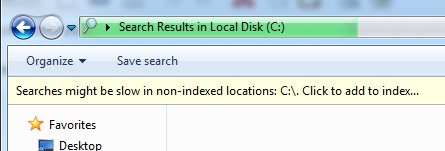
\includegraphics[scale=0.5]{images/windows7Example}
\caption{Example of the benefit of ordered (indexed) elements in Windows 7}
\label{figure:windows7Example}
\end{figure}

Though binary search presents a clear advantage over linear search, it only works
if the collection has been sorted.\footnote{Binary search also only works when
searching an array with random access to its elements.  The performance of binary
search cannot generally be realized with data structures such as linked lists or 
unordered sets.}  Thus, we now turn our attention to the problem of sorting
a collection.

\section{Sorting}
\index{sorting}

Sorting a collection of data is another fundamental data operation.  It is
conceptually simple, but is ubiquitous.  There are a large variety of
algorithms, data structures and applications built around the problem
of sorting.  As we've already seen, being able to sort a collection provides 
a huge speed up when searching for a particular element.  Sorting provides 
a natural way to store and organize data.  

\begin{problem}[Sorting]
~\\
\textbf{Given:} a collection of \emph{orderable} elements, $A =\{a_1, a_2, \ldots, a_n\}$\\
\textbf{Output:} $A$, sorted in ascending order
\end{problem}

The requirement that the collection be made of ``orderable'' elements can be
a bit technical\footnote{We require that $A$ be a \emph{total order} a 
partially ordered binary relation such that all pairs are comparable.}, but essentially 
we need to be guaranteed that given two elements, $a, b$ in the collection, 
we can determine whether $a < b$, $a = b$ or $a > b$.  If such a determination
cannot be made, then sorting is impossible.

Again, we can consider variations on this problem.  We may want our collection
to be sorted in descending order instead of ascending.\footnote{Technically, these are
referred to as \emph{non-decreasing} and \emph{non-increasing} respectively.  
This is because the collection could contain duplicate elements and not lead
to a strictly increasing or strictly decreasing ordering.} We may also want
the collection itself to be \emph{permuted} (that is, reordered) or we may
instead want a \emph{copy} of the collection to be created and sorted so that
the original is unchanged.

We will examine several standard sorting algorithms. Though there are dozens
of sorting algorithms, we will only focus on a few of the more common ones.  
As with 
searching, we can analyze a sorting algorithm based on the number of 
comparisons it makes in the worst, best, or average cases.  We may also look
at alternative resources or operations: how many swaps does the algorithm make?
How much extra memory is required?  Etc.

Though we will examine, analyze and compare several sorting algorithms, most
programming languages provide standard functionality to sort a collection of
elements.  It is generally preferable to use the functionality built into 
whatever language you're using rather that reimplementing your own.  Typically, 
these functions are well-designed, well-tested, optimized and more efficient
than any custom alternatives.

\subsection{Selection Sort}
\index{Selection Sort}
\index{sorting!Selection Sort}

The first sorting algorithm we'll examine is \emph{Selection Sort} which is
similar to the way a human would sort a collection of objects.  The basic idea
is that you search through the collection and find the minimal element 
(we say minimal and not minimum because there could be elements with the
same value).  Once we've found a minimal element, we can swap it with the
``first'' element, $a_1$, placing the minimal element where it belongs in
the collection.  

We repeat this process for the remaining elements, $a_2, \ldots, a_n$, 
finding the minimal element among these and swapping with $a_2$.  In 
general, if we have already sorted the first $i-1$ elements, 
$a_1, \ldots, a_{i-1}$ then we only need to examine the elements
$a_i, \ldots, a_n$ for the minimal element, swapping it with $a_i$.
We end this process after we have sorted the first $n-1$ elements, 
$a_1, \ldots, a_{n-1}$ since the last element $a_n$ will already
be where it needs to be.  We present Selection Sort as Algorithm 
\ref{algo:selectionSort}.  We illustrate the execution of Selection 
Sort in Figure \ref{figure:selectionSortExample}. 

    \begin{algorithm}[H]
     \Input{A collection $A = \{a_1, \ldots, a_n\}$}
     \Output{An array $A'$ containing all elements of $A$ in nondecreasing order}
     \For{$i = 1, \ldots, (n-1)$}{
       $a_{min} \leftarrow a_i$ \;
       \For{$j = (i+1), \ldots, n$}{
         \If{$a_{min} > a_j$}{ \label{algo:selectionSortComp}
           $min \leftarrow a_j$ \;
         }
       }
       swap $a_{min}$ and $a_i$ \;
     }
    \caption{Selection Sort}
    \label{algo:selectionSort}
    \end{algorithm}

%\documentclass[12pt]{scrbook}
%
%\usepackage{tikz}
%\usepackage{minted}
%\usetikzlibrary{decorations.pathreplacing,arrows}
%\usetikzlibrary{arrows,decorations.pathmorphing,backgrounds,positioning,fit,petri}
%
%\usepackage{fullpage}
%\usepackage{subfigure}
%\begin{document}
%
%
%Lorem Ipsum is simply dummy text of the printing and typesetting industry. Lorem Ipsum has been the industry's standard dummy text ever since the 1500s, when an unknown printer took a galley of type and scrambled it to make a type specimen book. It has survived not only five centuries, but also the leap into electronic typesetting, remaining essentially unchanged. It was popularised in the 1960s with the release of Letraset sheets containing Lorem Ipsum passages, and more recently with desktop publishing software like Aldus PageMaker including versions of Lorem Ipsum.
%




\begin{figure}
\centering

\subfigure[First iteration.  We find the minimal element, 0, at the last
index, swapping it with the first element.  At this point, the first
element is sorted.]{

\begin{tikzpicture}[scale=.65,transform shape]

\tikzset{>=stealth',shorten <=.2cm,>=stealth',shorten >=.2cm}
% size of each node
\def\sz{9mm}
% node style definition
\tikzstyle{block} = [
	draw, fill=black!10, rectangle,
	minimum height=\sz, minimum width=\sz ];
\tikzstyle{plain} = [draw=none,fill=none];

%\node[plain] at (-1.75, 1) { index };
%\node[plain] at (0*\sz,1.0) { 0 };
%\node[plain] at (1*\sz,1.0) { 1 };
%\node[plain] at (2*\sz,1.0) { 2 };
%\node[plain] at (3*\sz,1.0) { 3 };
%\node[plain] at (4*\sz,1.0) { 4 };
%\node[plain] at (5*\sz,1.0) { 5 };
%\node[plain] at (6*\sz,1.0) { 6 };
%\node[plain] at (7*\sz,1.0) { 7 };
%\node[plain] at (8*\sz,1.0) { 8 };
%\node[plain] at (-1.75, 0) { contents };
%

\node[block,fill=black!30] (a0) at (0*\sz,0) { 42 };
\node[block] (a1) at (1*\sz,0) { 4 };
\node[block] (a2) at (2*\sz,0) { 9 };
\node[block] (a3) at (3*\sz,0) { 4 };
\node[block] (a4) at (4*\sz,0) { 102 };
\node[block] (a5) at (5*\sz,0) { 34 };
\node[block] (a6) at (6*\sz,0) { 12 };
\node[block] (a7) at (7*\sz,0) { 2 };
\node[block,fill=green!30] (a8) at (8*\sz,0) { 0 };

\draw[<->] (a0.south) to [bend right] node[pos=.5,below] {swap} (a8.south);

\end{tikzpicture}~~~~~\begin{tikzpicture}[scale=.65,transform shape]
\draw[white] (0,0) rectangle (1, -2.05);

\tikzset{>=stealth',shorten <=.2cm,>=stealth',shorten >=.2cm}
\def\sz{9mm}
\tikzstyle{block} = [
	draw, fill=black!10, rectangle,
	minimum height=\sz, minimum width=\sz ];
\tikzstyle{plain} = [draw=none,fill=none];

\node[block,fill=black!50] (a0) at (0*\sz,0) { 0 };
\node[block] (a1) at (1*\sz,0) { 4 };
\node[block] (a2) at (2*\sz,0) { 9 };
\node[block] (a3) at (3*\sz,0) { 4 };
\node[block] (a4) at (4*\sz,0) { 102 };
\node[block] (a5) at (5*\sz,0) { 34 };
\node[block] (a6) at (6*\sz,0) { 12 };
\node[block] (a7) at (7*\sz,0) { 2 };
\node[block] (a8) at (8*\sz,0) { 42 };

\end{tikzpicture}

}

\subfigure[Second Iteration.  Now starting with the second element, the
minimal element among the remaining is found at the second to last element.
4 and 2 are swapped.  At this point, the first two elements are sorted.]{

\begin{tikzpicture}[scale=.65,transform shape]

\tikzset{>=stealth',shorten <=.2cm,>=stealth',shorten >=.2cm}
\def\sz{9mm}
\tikzstyle{block} = [
	draw, fill=black!10, rectangle,
	minimum height=\sz, minimum width=\sz ];
\tikzstyle{plain} = [draw=none,fill=none];

\node[block,fill=black!50] (a0) at (0*\sz,0) { 0 };
\node[block,fill=black!30] (a1) at (1*\sz,0) { 4 };
\node[block] (a2) at (2*\sz,0) { 9 };
\node[block] (a3) at (3*\sz,0) { 4 };
\node[block] (a4) at (4*\sz,0) { 102 };
\node[block] (a5) at (5*\sz,0) { 34 };
\node[block] (a6) at (6*\sz,0) { 12 };
\node[block,fill=green!30] (a7) at (7*\sz,0) { 2 };
\node[block] (a8) at (8*\sz,0) { 42 };

\draw[<->] (a1.south) to [bend right] node[pos=.5,below] {swap} (a7.south);

\end{tikzpicture}~~~~~\begin{tikzpicture}[scale=.65,transform shape]
\draw[white] (0,0) rectangle (1, -1.75);

\tikzset{>=stealth',shorten <=.2cm,>=stealth',shorten >=.2cm}
\def\sz{9mm}
\tikzstyle{block} = [
	draw, fill=black!10, rectangle,
	minimum height=\sz, minimum width=\sz ];
\tikzstyle{plain} = [draw=none,fill=none];

\node[block,fill=black!50] (a0) at (0*\sz,0) { 0 };
\node[block,fill=black!50] (a1) at (1*\sz,0) { 2 };
\node[block] (a2) at (2*\sz,0) { 9 };
\node[block] (a3) at (3*\sz,0) { 4 };
\node[block] (a4) at (4*\sz,0) { 102 };
\node[block] (a5) at (5*\sz,0) { 34 };
\node[block] (a6) at (6*\sz,0) { 12 };
\node[block] (a7) at (7*\sz,0) { 4 };
\node[block] (a8) at (8*\sz,0) { 42 };

%\draw[<->] (a1.south) to [bend right] node[pos=.5,below] {swap} (a7.south);

\end{tikzpicture}

}

\subfigure[Third iteration.  Since we are using the strictly-less than comparison, the first 4 is the minimal element and swapped with 9.]{

\begin{tikzpicture}[scale=.65,transform shape]

\tikzset{>=stealth',shorten <=.2cm,>=stealth',shorten >=.2cm}
\def\sz{9mm}
\tikzstyle{block} = [
	draw, fill=black!10, rectangle,
	minimum height=\sz, minimum width=\sz ];
\tikzstyle{plain} = [draw=none,fill=none];

\node[block,fill=black!50] (a0) at (0*\sz,0) { 0 };
\node[block,fill=black!50] (a1) at (1*\sz,0) { 2 };
\node[block,fill=black!30] (a2) at (2*\sz,0) { 9 };
\node[block,fill=green!30] (a3) at (3*\sz,0) { 4 };
\node[block] (a4) at (4*\sz,0) { 102 };
\node[block] (a5) at (5*\sz,0) { 34 };
\node[block] (a6) at (6*\sz,0) { 12 };
\node[block] (a7) at (7*\sz,0) { 4 };
\node[block] (a8) at (8*\sz,0) { 42 };

\draw[<->] (a2.south) to [bend right] node[pos=.5,below] {swap} (a3.south);

\end{tikzpicture}~~~~~\begin{tikzpicture}[scale=.65,transform shape]
\draw[white] (0,0) rectangle (1, -1.1);

\tikzset{>=stealth',shorten <=.2cm,>=stealth',shorten >=.2cm}
\def\sz{9mm}
\tikzstyle{block} = [
	draw, fill=black!10, rectangle,
	minimum height=\sz, minimum width=\sz ];
\tikzstyle{plain} = [draw=none,fill=none];

\node[block,fill=black!50] (a0) at (0*\sz,0) { 0 };
\node[block,fill=black!50] (a1) at (1*\sz,0) { 2 };
\node[block,fill=black!50] (a2) at (2*\sz,0) { 4 };
\node[block] (a3) at (3*\sz,0) { 9 };
\node[block] (a4) at (4*\sz,0) { 102 };
\node[block] (a5) at (5*\sz,0) { 34 };
\node[block] (a6) at (6*\sz,0) { 12 };
\node[block] (a7) at (7*\sz,0) { 4 };
\node[block] (a8) at (8*\sz,0) { 42 };

%\draw[<->] (a1.south) to [bend right] node[pos=.5,below] {swap} (a7.south);

\end{tikzpicture}

}

\subfigure[Fourth iteration.  At this point, the first 3 elements are
sorted.  We find the minimal element (the other 4) and swap it with
9.  At the end of this iteration, the first 4 elements are sorted.]{

\begin{tikzpicture}[scale=.65,transform shape]

\tikzset{>=stealth',shorten <=.2cm,>=stealth',shorten >=.2cm}
\def\sz{9mm}
\tikzstyle{block} = [
	draw, fill=black!10, rectangle,
	minimum height=\sz, minimum width=\sz ];
\tikzstyle{plain} = [draw=none,fill=none];

\node[block,fill=black!50] (a0) at (0*\sz,0) { 0 };
\node[block,fill=black!50] (a1) at (1*\sz,0) { 2 };
\node[block,fill=black!50] (a2) at (2*\sz,0) { 4 };
\node[block,fill=black!30] (a3) at (3*\sz,0) { 9 };
\node[block] (a4) at (4*\sz,0) { 102 };
\node[block] (a5) at (5*\sz,0) { 34 };
\node[block] (a6) at (6*\sz,0) { 12 };
\node[block,fill=green!30] (a7) at (7*\sz,0) { 4 };
\node[block] (a8) at (8*\sz,0) { 42 };

\draw[<->] (a3.south) to [bend right] node[pos=.5,below] {swap} (a7.south);

\end{tikzpicture}~~~~~\begin{tikzpicture}[scale=.65,transform shape]
\draw[white] (0,0) rectangle (1, -1.5);

\tikzset{>=stealth',shorten <=.2cm,>=stealth',shorten >=.2cm}
\def\sz{9mm}
\tikzstyle{block} = [
	draw, fill=black!10, rectangle,
	minimum height=\sz, minimum width=\sz ];
\tikzstyle{plain} = [draw=none,fill=none];

\node[block,fill=black!50] (a0) at (0*\sz,0) { 0 };
\node[block,fill=black!50] (a1) at (1*\sz,0) { 2 };
\node[block,fill=black!50] (a2) at (2*\sz,0) { 4 };
\node[block,fill=black!50] (a3) at (3*\sz,0) { 4 };
\node[block] (a4) at (4*\sz,0) { 102 };
\node[block] (a5) at (5*\sz,0) { 34 };
\node[block] (a6) at (6*\sz,0) { 12 };
\node[block] (a7) at (7*\sz,0) { 9 };
\node[block] (a8) at (8*\sz,0) { 42 };

%\draw[<->] (a1.south) to [bend right] node[pos=.5,below] {swap} (a7.south);

\end{tikzpicture}

}

\subfigure[Fifth iteration.  The 9 is swapped with 102, sorting
the first 5 elements.]{

\begin{tikzpicture}[scale=.65,transform shape]

\tikzset{>=stealth',shorten <=.2cm,>=stealth',shorten >=.2cm}
\def\sz{9mm}
\tikzstyle{block} = [
	draw, fill=black!10, rectangle,
	minimum height=\sz, minimum width=\sz ];
\tikzstyle{plain} = [draw=none,fill=none];

\node[block,fill=black!50] (a0) at (0*\sz,0) { 0 };
\node[block,fill=black!50] (a1) at (1*\sz,0) { 2 };
\node[block,fill=black!50] (a2) at (2*\sz,0) { 4 };
\node[block,fill=black!50] (a3) at (3*\sz,0) { 4 };
\node[block,fill=black!30] (a4) at (4*\sz,0) { 102 };
\node[block] (a5) at (5*\sz,0) { 34 };
\node[block] (a6) at (6*\sz,0) { 12 };
\node[block,fill=green!30] (a7) at (7*\sz,0) { 9 };
\node[block] (a8) at (8*\sz,0) { 42 };

\draw[<->] (a4.south) to [bend right] node[pos=.5,below] {swap} (a7.south);

\end{tikzpicture}~~~~~\begin{tikzpicture}[scale=.65,transform shape]
\draw[white] (0,0) rectangle (1, -1.4);

\tikzset{>=stealth',shorten <=.2cm,>=stealth',shorten >=.2cm}
\def\sz{9mm}
\tikzstyle{block} = [
	draw, fill=black!10, rectangle,
	minimum height=\sz, minimum width=\sz ];
\tikzstyle{plain} = [draw=none,fill=none];

\node[block,fill=black!50] (a0) at (0*\sz,0) { 0 };
\node[block,fill=black!50] (a1) at (1*\sz,0) { 2 };
\node[block,fill=black!50] (a2) at (2*\sz,0) { 4 };
\node[block,fill=black!50] (a3) at (3*\sz,0) { 4 };
\node[block,fill=black!50] (a4) at (4*\sz,0) { 9 };
\node[block] (a5) at (5*\sz,0) { 34 };
\node[block] (a6) at (6*\sz,0) { 12 };
\node[block] (a7) at (7*\sz,0) { 102 };
\node[block] (a8) at (8*\sz,0) { 42 };

%\draw[<->] (a1.south) to [bend right] node[pos=.5,below] {swap} (a7.south);

\end{tikzpicture}

}

\subfigure[Sixth iteration.  12 is swapped with 34.]{

\begin{tikzpicture}[scale=.65,transform shape]

\tikzset{>=stealth',shorten <=.2cm,>=stealth',shorten >=.2cm}
\def\sz{9mm}
\tikzstyle{block} = [
	draw, fill=black!10, rectangle,
	minimum height=\sz, minimum width=\sz ];
\tikzstyle{plain} = [draw=none,fill=none];

\node[block,fill=black!50] (a0) at (0*\sz,0) { 0 };
\node[block,fill=black!50] (a1) at (1*\sz,0) { 2 };
\node[block,fill=black!50] (a2) at (2*\sz,0) { 4 };
\node[block,fill=black!50] (a3) at (3*\sz,0) { 4 };
\node[block,fill=black!50] (a4) at (4*\sz,0) { 9 };
\node[block,fill=black!30] (a5) at (5*\sz,0) { 34 };
\node[block,fill=green!30] (a6) at (6*\sz,0) { 12 };
\node[block] (a7) at (7*\sz,0) { 102 };
\node[block] (a8) at (8*\sz,0) { 42 };

\draw[<->] (a5.south) to [bend right] node[pos=.5,below] {swap} (a6.south);

\end{tikzpicture}~~~~~\begin{tikzpicture}[scale=.65,transform shape]
\draw[white] (0,0) rectangle (1, -1.1);

\tikzset{>=stealth',shorten <=.2cm,>=stealth',shorten >=.2cm}
\def\sz{9mm}
\tikzstyle{block} = [
	draw, fill=black!10, rectangle,
	minimum height=\sz, minimum width=\sz ];
\tikzstyle{plain} = [draw=none,fill=none];

\node[block,fill=black!50] (a0) at (0*\sz,0) { 0 };
\node[block,fill=black!50] (a1) at (1*\sz,0) { 2 };
\node[block,fill=black!50] (a2) at (2*\sz,0) { 4 };
\node[block,fill=black!50] (a3) at (3*\sz,0) { 4 };
\node[block,fill=black!50] (a4) at (4*\sz,0) { 9 };
\node[block,fill=black!50] (a5) at (5*\sz,0) { 12 };
\node[block] (a6) at (6*\sz,0) { 34 };
\node[block] (a7) at (7*\sz,0) { 102 };
\node[block] (a8) at (8*\sz,0) { 42 };

%\draw[<->] (a1.south) to [bend right] node[pos=.5,below] {swap} (a7.south);

\end{tikzpicture}

}

\subfigure[Seventh iteration.  34 ends up being the minimal element
and we essentially swap it with itself.  Even though the ``current''
element was also the minimal element, we still had to compare
the current element with all other elements; in this case we made 2
comparisons.]{

\begin{tikzpicture}[scale=.65,transform shape]

\tikzset{>=stealth',shorten <=.2cm,>=stealth',shorten >=.2cm}
\def\sz{9mm}
\tikzstyle{block} = [
	draw, fill=black!10, rectangle,
	minimum height=\sz, minimum width=\sz ];
\tikzstyle{plain} = [draw=none,fill=none];

\node[block,fill=black!50] (a0) at (0*\sz,0) { 0 };
\node[block,fill=black!50] (a1) at (1*\sz,0) { 2 };
\node[block,fill=black!50] (a2) at (2*\sz,0) { 4 };
\node[block,fill=black!50] (a3) at (3*\sz,0) { 4 };
\node[block,fill=black!50] (a4) at (4*\sz,0) { 9 };
\node[block,fill=black!50] (a5) at (5*\sz,0) { 12 };
\node[block,fill=green!30] (a6) at (6*\sz,0) { 34 };
\node[block] (a7) at (7*\sz,0) { 102 };
\node[block] (a8) at (8*\sz,0) { 42 };

\node[below of=a6] {swap} ;
%\draw[<->] (a6.south) to [bend right] node[pos=.5,below] {swap} (a6.south);

\end{tikzpicture}~~~~~\begin{tikzpicture}[scale=.65,transform shape]
\draw[white] (0,0) rectangle (1, -1.2);

\tikzset{>=stealth',shorten <=.2cm,>=stealth',shorten >=.2cm}
\def\sz{9mm}
\tikzstyle{block} = [
	draw, fill=black!10, rectangle,
	minimum height=\sz, minimum width=\sz ];
\tikzstyle{plain} = [draw=none,fill=none];

\node[block,fill=black!50] (a0) at (0*\sz,0) { 0 };
\node[block,fill=black!50] (a1) at (1*\sz,0) { 2 };
\node[block,fill=black!50] (a2) at (2*\sz,0) { 4 };
\node[block,fill=black!50] (a3) at (3*\sz,0) { 4 };
\node[block,fill=black!50] (a4) at (4*\sz,0) { 9 };
\node[block,fill=black!50] (a5) at (5*\sz,0) { 12 };
\node[block,fill=black!50] (a6) at (6*\sz,0) { 34 };
\node[block] (a7) at (7*\sz,0) { 102 };
\node[block] (a8) at (8*\sz,0) { 42 };

%\draw[<->] (a1.south) to [bend right] node[pos=.5,below] {swap} (a7.south);

\end{tikzpicture}

}

\subfigure[Eighth iteration.  This is the final iteration, we swap
42 and 102.  After this iteration, the final element, 102 is already
where it needs to be.]{

\begin{tikzpicture}[scale=.65,transform shape]

\tikzset{>=stealth',shorten <=.2cm,>=stealth',shorten >=.2cm}
\def\sz{9mm}
\tikzstyle{block} = [
	draw, fill=black!10, rectangle,
	minimum height=\sz, minimum width=\sz ];
\tikzstyle{plain} = [draw=none,fill=none];

\node[block,fill=black!50] (a0) at (0*\sz,0) { 0 };
\node[block,fill=black!50] (a1) at (1*\sz,0) { 2 };
\node[block,fill=black!50] (a2) at (2*\sz,0) { 4 };
\node[block,fill=black!50] (a3) at (3*\sz,0) { 4 };
\node[block,fill=black!50] (a4) at (4*\sz,0) { 9 };
\node[block,fill=black!50] (a5) at (5*\sz,0) { 12 };
\node[block,fill=black!50] (a6) at (6*\sz,0) { 34 };
\node[block,fill=black!30] (a7) at (7*\sz,0) { 102 };
\node[block,fill=green!30] (a8) at (8*\sz,0) { 42 };

\draw[<->] (a7.south) to [bend right] node[pos=.5,below] {swap} (a8.south);

\end{tikzpicture}~~~~~\begin{tikzpicture}[scale=.65,transform shape]
\draw[white] (0,0) rectangle (1, -1.1);

\tikzset{>=stealth',shorten <=.2cm,>=stealth',shorten >=.2cm}
\def\sz{9mm}
\tikzstyle{block} = [
	draw, fill=black!10, rectangle,
	minimum height=\sz, minimum width=\sz ];
\tikzstyle{plain} = [draw=none,fill=none];

\node[block,fill=black!50] (a0) at (0*\sz,0) { 0 };
\node[block,fill=black!50] (a1) at (1*\sz,0) { 2 };
\node[block,fill=black!50] (a2) at (2*\sz,0) { 4 };
\node[block,fill=black!50] (a3) at (3*\sz,0) { 4 };
\node[block,fill=black!50] (a4) at (4*\sz,0) { 9 };
\node[block,fill=black!50] (a5) at (5*\sz,0) { 12 };
\node[block,fill=black!50] (a6) at (6*\sz,0) { 34 };
\node[block,fill=black!50] (a7) at (7*\sz,0) { 42 };
\node[block] (a8) at (8*\sz,0) { 102 };

%\draw[<->] (a1.south) to [bend right] node[pos=.5,below] {swap} (a7.south);

\end{tikzpicture}

}

\caption[Selection Sort Example]{Example execution of Selection Sort.}
\label{figure:selectionSortExample}

\end{figure}


%\end{document}



\subsubsection{Analysis}
\index{Selection Sort!analysis}

We now analyze Selection Sort to determine how complex it is.  First, the
elementary operation is the comparison on line \ref{algo:selectionSortComp}.
We need to determine how many times this line is executed with respect
to the size of the input, $n$.  Observe that on the $i$-th iteration, the first
$i-1$ elements are sorted and we need not make any comparisons among
them.  We start by assuming that the $a_i$ is the minimum element and
compare it to the remaining $n-i$ elements, requiring $n-i$ comparisons,
to find the minimal element.  For example, in the first iteration we
make $n-1$ comparisons, the second we make $n-2$, etc.  The last
iteration we make only 1 comparison.  Totaling these all up gives us
  $$(n-1) + (n-2) + (n-3) + \cdots + 3 + 2 + 1$$
Which can be rewritten as 
  $$\sum_{i=1}^{n-1} i = 1 + 2 + 3 + \cdots + (n-2) + (n-1)$$
We can use Gauss's Formula to solve this summation.

\index{Gauss's Formula}
\begin{theorem}[Gauss's Formula]
The sum of integers $1$ up to $n$ can be written as follows.
$$\sum_{i=1}^{n} i = 1 + 2 + 3 + \cdots + (n-1) + n = \frac{n(n+1)}{2}$$
\end{theorem}

In Selection Sort, the number of comparisons doesn't sum up to $n$, 
only $n-1$.  Substituting this in gives us 

$$\sum_{i=1}^{n-1} i = \frac{n(n-1)}{2}$$

Another way to analyze the code is to count the number of comparisons
with respect to the for loop index variables.  In particular, there
is one comparison made on line 4.  Line 4 itself is executed once
for each time the inner for loop on line 3 executes which executes 
for $j$ running from $i+1$ up to $n$.  Line 3 and the entire inner
for loop executes once for each time the outer for loop executes, 
that is for $i$ running from $1$ up to $n-1$. This gives us the 
following summation.
  $$\underbrace{\sum_{i=1}^{n-1} \, \underbrace{\sum_{j=i+1}^{n} \, \underbrace{
  \vphantom{\left(\frac{a^{0.3}}{b}\right)}
1}_{\textrm{line 4}}}_{\textrm{line 3}}}_{\textrm{line 1}}$$
Solving this summation gives us:
\begin{align*}
  \sum_{i=1}^{n-1} \sum_{j=i+1}^{n} 1 & = \sum_{i=1}^{n-1} n-i \\
  ~ & = \sum_{i=1}^{n-1} n - \sum_{i=1}^{n-1} i \\
  ~ & = n(n-1) - \frac{n(n-1)}{2}\\
  ~ & = \frac{n(n-1)}{2}\\
\end{align*}

This illustrates that Selection Sort is a \emph{quadratic} sorting algorithm, 
requiring roughly $n^2$ comparisons to sort an array of $n$ elements.
We analyze this further below.

\subsection{Insertion Sort}
\index{Insertion Sort}
\index{sorting!Insertion Sort}

Another basic sorting algorithm is \emph{Insertion Sort} which works 
slightly differently than Selection Sort.  Rather than finding a minimal
element and swapping with the ``current'' element, the current element
is \emph{inserted} in the list where it belongs.

If we consider just the first element, the collection is sorted by
definition.  Now consider the second element: either its greater than
the first element and so is already sorted, or it is less than the first element
and needs to be swapped.  In either case, the first two elements are now
sorted.  If we continue this, then on the $i$-th iteration, the first
$i$ elements, $a_1, \ldots, a_i$ are sorted (just as with Selection Sort).
Now consider the $(i+1)$-th element: we will \emph{insert} it amongst
the elements $a_1, \ldots, a_i$ where it needs to be.

We insert the ``current'' element, $a_{i+1}$ by comparing it to $a_i$: 
if $a_i > a_{i+1}$, then we swap them.  We keep comparing the current
element to the one immediately to its left, shifting the current element
down the collection until we find an element that is less than or equal 
to the
current element at which point we stop.  Now the elements $a_1, \ldots, a_{i+1}$
are now sorted.  In contrast to Selection Sort, we \emph{do} need to process
the last element as it might not be where it needs to be.  The
full pseudocode is presented in Algorithm \ref{algo:insertionSort}.
An example of an execution of Insertion Sort can be found in Figure\ref{figure:insertionSortExample}.

\begin{algorithm}[H]
  \Input{A collection $A = \{a_1, \ldots, a_n\}$}
  \Output{An array $A'$ containing all elements of $A$ in nondecreasing order}
     \For{$i = 2, \ldots, n$}{
       $x \leftarrow a_i$ \;
       $j \leftarrow i$ \;
       \While{$j > 1$ and $a_{j-1} > x$}{
         $a_j \leftarrow a_{j-1}$ \;
         decrement $j$ \;
       }
       $a_j \leftarrow x$ \;
     }
\caption{Insertion Sort}
\label{algo:insertionSort}
\end{algorithm}

%\documentclass[12pt]{scrbook}
%
%\usepackage{tikz}
%\usepackage{minted}
%\usetikzlibrary{decorations.pathreplacing,arrows}
%\usetikzlibrary{arrows,decorations.pathmorphing,backgrounds,positioning,fit,petri}
%
%\usepackage{fullpage}
%\usepackage{subfigure}
%\begin{document}
%
%
%Lorem Ipsum is simply dummy text of the printing and typesetting industry. Lorem Ipsum has been the industry's standard dummy text ever since the 1500s, when an unknown printer took a galley of type and scrambled it to make a type specimen book. It has survived not only five centuries, but also the leap into electronic typesetting, remaining essentially unchanged. It was popularised in the 1960s with the release of Letraset sheets containing Lorem Ipsum passages, and more recently with desktop publishing software like Aldus PageMaker including versions of Lorem Ipsum.
%




\begin{figure}
\centering

\subfigure[First iteration.  We insert 4 in front of 42, requiring 1 
comparison.]{

\begin{tikzpicture}[scale=.65,transform shape]

\tikzset{>=stealth',shorten <=.2cm,>=stealth',shorten >=.2cm}
% size of each node
\def\sz{9mm}
% node style definition
\tikzstyle{block} = [
	draw, fill=black!10, rectangle,
	minimum height=\sz, minimum width=\sz ];
\tikzstyle{plain} = [draw=none,fill=none];

%\node[plain] at (-1.75, 1) { index };
%\node[plain] at (0*\sz,1.0) { 0 };
%\node[plain] at (1*\sz,1.0) { 1 };
%\node[plain] at (2*\sz,1.0) { 2 };
%\node[plain] at (3*\sz,1.0) { 3 };
%\node[plain] at (4*\sz,1.0) { 4 };
%\node[plain] at (5*\sz,1.0) { 5 };
%\node[plain] at (6*\sz,1.0) { 6 };
%\node[plain] at (7*\sz,1.0) { 7 };
%\node[plain] at (8*\sz,1.0) { 8 };
%\node[plain] at (-1.75, 0) { contents };
%

\node[block,fill=black!50] (a0) at (0*\sz,0) { 42 };
\node[block,fill=green!30] (a1) at (1*\sz,0) { 4 };
\node[block] (a2) at (2*\sz,0) { 9 };
\node[block] (a3) at (3*\sz,0) { 4 };
\node[block] (a4) at (4*\sz,0) { 102 };
\node[block] (a5) at (5*\sz,0) { 34 };
\node[block] (a6) at (6*\sz,0) { 12 };
\node[block] (a7) at (7*\sz,0) { 2 };
\node[block] (a8) at (8*\sz,0) { 0 };

\draw[<-] (a0.north) to [in=90,out=90,looseness=3] node[pos=.5,above] {} (a1.north);

\end{tikzpicture}~~~~~\begin{tikzpicture}[scale=.65,transform shape]

\tikzset{>=stealth',shorten <=.2cm,>=stealth',shorten >=.2cm}
\def\sz{9mm}
\tikzstyle{block} = [
	draw, fill=black!10, rectangle,
	minimum height=\sz, minimum width=\sz ];
\tikzstyle{plain} = [draw=none,fill=none];

\node[block,fill=black!50] (a0) at (0*\sz,0) { 4 };
\node[block,fill=black!50] (a1) at (1*\sz,0) { 42 };
\node[block] (a2) at (2*\sz,0) { 9 };
\node[block] (a3) at (3*\sz,0) { 4 };
\node[block] (a4) at (4*\sz,0) { 102 };
\node[block] (a5) at (5*\sz,0) { 34 };
\node[block] (a6) at (6*\sz,0) { 12 };
\node[block] (a7) at (7*\sz,0) { 2 };
\node[block] (a8) at (8*\sz,0) { 0 };

\end{tikzpicture}

}

\subfigure[Second iteration.  The first two elements are sorted, we insert
9 by making two comparisons: to find that it is less than 42, bug greater
than 4.  At the end of the iteration, the first three elements are
sorted.]{

\begin{tikzpicture}[scale=.65,transform shape]

\tikzset{>=stealth',shorten <=.2cm,>=stealth',shorten >=.2cm}
% size of each node
\def\sz{9mm}
% node style definition
\tikzstyle{block} = [
	draw, fill=black!10, rectangle,
	minimum height=\sz, minimum width=\sz ];
\tikzstyle{plain} = [draw=none,fill=none];

%\node[plain] at (-1.75, 1) { index };
%\node[plain] at (0*\sz,1.0) { 0 };
%\node[plain] at (1*\sz,1.0) { 1 };
%\node[plain] at (2*\sz,1.0) { 2 };
%\node[plain] at (3*\sz,1.0) { 3 };
%\node[plain] at (4*\sz,1.0) { 4 };
%\node[plain] at (5*\sz,1.0) { 5 };
%\node[plain] at (6*\sz,1.0) { 6 };
%\node[plain] at (7*\sz,1.0) { 7 };
%\node[plain] at (8*\sz,1.0) { 8 };
%\node[plain] at (-1.75, 0) { contents };
%

\node[block,fill=black!50] (a0) at (0*\sz,0) { 4 };
\node[block,fill=black!50] (a1) at (1*\sz,0) { 42 };
\node[block,fill=green!30] (a2) at (2*\sz,0) { 9 };
\node[block] (a3) at (3*\sz,0) { 4 };
\node[block] (a4) at (4*\sz,0) { 102 };
\node[block] (a5) at (5*\sz,0) { 34 };
\node[block] (a6) at (6*\sz,0) { 12 };
\node[block] (a7) at (7*\sz,0) { 2 };
\node[block] (a8) at (8*\sz,0) { 0 };

\draw[<-,dotted] (a0.north) to [in=90,out=90,looseness=3] node[pos=.5,above] {2}(a2.north);
\draw[<-] (a1.north) to [in=90,out=90,looseness=3] node[pos=.5,above] {1} (a2.north);

\end{tikzpicture}~~~~~\begin{tikzpicture}[scale=.65,transform shape]

\tikzset{>=stealth',shorten <=.2cm,>=stealth',shorten >=.2cm}
\def\sz{9mm}
\tikzstyle{block} = [
	draw, fill=black!10, rectangle,
	minimum height=\sz, minimum width=\sz ];
\tikzstyle{plain} = [draw=none,fill=none];

\node[block,fill=black!50] (a0) at (0*\sz,0) { 4 };
\node[block,fill=black!50] (a1) at (1*\sz,0) { 9 };
\node[block,fill=black!50] (a2) at (2*\sz,0) { 42 };
\node[block] (a3) at (3*\sz,0) { 4 };
\node[block] (a4) at (4*\sz,0) { 102 };
\node[block] (a5) at (5*\sz,0) { 34 };
\node[block] (a6) at (6*\sz,0) { 12 };
\node[block] (a7) at (7*\sz,0) { 2 };
\node[block] (a8) at (8*\sz,0) { 0 };

\end{tikzpicture}

}

\subfigure[Third iteration.  The first three elements are sorted, we
insert the second four by making 3 comparisons.]{

\begin{tikzpicture}[scale=.65,transform shape]

\tikzset{>=stealth',shorten <=.2cm,>=stealth',shorten >=.2cm}
% size of each node
\def\sz{9mm}
% node style definition
\tikzstyle{block} = [
	draw, fill=black!10, rectangle,
	minimum height=\sz, minimum width=\sz ];
\tikzstyle{plain} = [draw=none,fill=none];

%\node[plain] at (-1.75, 1) { index };
%\node[plain] at (0*\sz,1.0) { 0 };
%\node[plain] at (1*\sz,1.0) { 1 };
%\node[plain] at (2*\sz,1.0) { 2 };
%\node[plain] at (3*\sz,1.0) { 3 };
%\node[plain] at (4*\sz,1.0) { 4 };
%\node[plain] at (5*\sz,1.0) { 5 };
%\node[plain] at (6*\sz,1.0) { 6 };
%\node[plain] at (7*\sz,1.0) { 7 };
%\node[plain] at (8*\sz,1.0) { 8 };
%\node[plain] at (-1.75, 0) { contents };
%

\node[block,fill=black!50] (a0) at (0*\sz,0) { 4 };
\node[block,fill=black!50] (a1) at (1*\sz,0) { 9 };
\node[block,fill=black!50] (a2) at (2*\sz,0) { 42 };
\node[block,fill=green!50] (a3) at (3*\sz,0) { 4 };
\node[block] (a4) at (4*\sz,0) { 102 };
\node[block] (a5) at (5*\sz,0) { 34 };
\node[block] (a6) at (6*\sz,0) { 12 };
\node[block] (a7) at (7*\sz,0) { 2 };
\node[block] (a8) at (8*\sz,0) { 0 };

\draw[<-,dotted] (a0.north) to [in=90,out=90,looseness=3] node[pos=.5,above] {3}(a3.north);
\draw[<-] (a1.north) to [in=90,out=90,looseness=3] node[pos=.5,above] {2}(a3.north);
\draw[<-] (a2.north) to [in=90,out=90,looseness=3] node[pos=.5,above] {1} (a3.north);

\end{tikzpicture}~~~~~\begin{tikzpicture}[scale=.65,transform shape]

\tikzset{>=stealth',shorten <=.2cm,>=stealth',shorten >=.2cm}
\def\sz{9mm}
\tikzstyle{block} = [
	draw, fill=black!10, rectangle,
	minimum height=\sz, minimum width=\sz ];
\tikzstyle{plain} = [draw=none,fill=none];

\node[block,fill=black!50] (a0) at (0*\sz,0) { 4 };
\node[block,fill=black!50] (a1) at (1*\sz,0) { 4 };
\node[block,fill=black!50] (a2) at (2*\sz,0) { 9 };
\node[block,fill=black!50] (a3) at (3*\sz,0) { 42 };
\node[block] (a4) at (4*\sz,0) { 102 };
\node[block] (a5) at (5*\sz,0) { 34 };
\node[block] (a6) at (6*\sz,0) { 12 };
\node[block] (a7) at (7*\sz,0) { 2 };
\node[block] (a8) at (8*\sz,0) { 0 };

\end{tikzpicture}

}

\subfigure[Fourth iteration.  Here, only one comparison is necessary
to find that 102 is already where it needs to be.]{

\begin{tikzpicture}[scale=.65,transform shape]

\tikzset{>=stealth',shorten <=.2cm,>=stealth',shorten >=.2cm}
% size of each node
\def\sz{9mm}
% node style definition
\tikzstyle{block} = [
	draw, fill=black!10, rectangle,
	minimum height=\sz, minimum width=\sz ];
\tikzstyle{plain} = [draw=none,fill=none];

%\node[plain] at (-1.75, 1) { index };
%\node[plain] at (0*\sz,1.0) { 0 };
%\node[plain] at (1*\sz,1.0) { 1 };
%\node[plain] at (2*\sz,1.0) { 2 };
%\node[plain] at (3*\sz,1.0) { 3 };
%\node[plain] at (4*\sz,1.0) { 4 };
%\node[plain] at (5*\sz,1.0) { 5 };
%\node[plain] at (6*\sz,1.0) { 6 };
%\node[plain] at (7*\sz,1.0) { 7 };
%\node[plain] at (8*\sz,1.0) { 8 };
%\node[plain] at (-1.75, 0) { contents };
%

\node[block,fill=black!50] (a0) at (0*\sz,0) { 4 };
\node[block,fill=black!50] (a1) at (1*\sz,0) { 4 };
\node[block,fill=black!50] (a2) at (2*\sz,0) { 9 };
\node[block,fill=black!50] (a3) at (3*\sz,0) { 42 };
\node[block,fill=green!50] (a4) at (4*\sz,0) { 102 };
\node[block] (a5) at (5*\sz,0) { 34 };
\node[block] (a6) at (6*\sz,0) { 12 };
\node[block] (a7) at (7*\sz,0) { 2 };
\node[block] (a8) at (8*\sz,0) { 0 };

\draw[<-] (a3.north) to [in=90,out=90,looseness=3] node[pos=.5,above] {1} (a4.north);

\end{tikzpicture}~~~~~\begin{tikzpicture}[scale=.65,transform shape]

\tikzset{>=stealth',shorten <=.2cm,>=stealth',shorten >=.2cm}
\def\sz{9mm}
\tikzstyle{block} = [
	draw, fill=black!10, rectangle,
	minimum height=\sz, minimum width=\sz ];
\tikzstyle{plain} = [draw=none,fill=none];

\node[block,fill=black!50] (a0) at (0*\sz,0) { 4 };
\node[block,fill=black!50] (a1) at (1*\sz,0) { 4 };
\node[block,fill=black!50] (a2) at (2*\sz,0) { 9 };
\node[block,fill=black!50] (a3) at (3*\sz,0) { 42 };
\node[block,fill=black!50] (a4) at (4*\sz,0) { 102 };
\node[block] (a5) at (5*\sz,0) { 34 };
\node[block] (a6) at (6*\sz,0) { 12 };
\node[block] (a7) at (7*\sz,0) { 2 };
\node[block] (a8) at (8*\sz,0) { 0 };

\end{tikzpicture}

}

\subfigure[Fifth iteration.  Here, 3 comparisons are necessary to insert
34 between 9 and 42.]{

\begin{tikzpicture}[scale=.65,transform shape]

\tikzset{>=stealth',shorten <=.2cm,>=stealth',shorten >=.2cm}
% size of each node
\def\sz{9mm}
% node style definition
\tikzstyle{block} = [
	draw, fill=black!10, rectangle,
	minimum height=\sz, minimum width=\sz ];
\tikzstyle{plain} = [draw=none,fill=none];

%\node[plain] at (-1.75, 1) { index };
%\node[plain] at (0*\sz,1.0) { 0 };
%\node[plain] at (1*\sz,1.0) { 1 };
%\node[plain] at (2*\sz,1.0) { 2 };
%\node[plain] at (3*\sz,1.0) { 3 };
%\node[plain] at (4*\sz,1.0) { 4 };
%\node[plain] at (5*\sz,1.0) { 5 };
%\node[plain] at (6*\sz,1.0) { 6 };
%\node[plain] at (7*\sz,1.0) { 7 };
%\node[plain] at (8*\sz,1.0) { 8 };
%\node[plain] at (-1.75, 0) { contents };
%

\node[block,fill=black!50] (a0) at (0*\sz,0) { 4 };
\node[block,fill=black!50] (a1) at (1*\sz,0) { 4 };
\node[block,fill=black!50] (a2) at (2*\sz,0) { 9 };
\node[block,fill=black!50] (a3) at (3*\sz,0) { 42 };
\node[block,fill=black!50] (a4) at (4*\sz,0) { 102 };
\node[block,fill=green!50] (a5) at (5*\sz,0) { 34 };
\node[block] (a6) at (6*\sz,0) { 12 };
\node[block] (a7) at (7*\sz,0) { 2 };
\node[block] (a8) at (8*\sz,0) { 0 };

\draw[<-] (a4.north) to [in=90,out=90,looseness=2] node[pos=.5,above] {1} (a5.north);
\draw[<-] (a3.north) to [in=90,out=90,looseness=2] node[pos=.5,above] {2} (a5.north);
\draw[<-,dotted] (a2.north) to [in=90,out=90,looseness=2] node[pos=.5,above] {3} (a5.north);

\end{tikzpicture}~~~~~\begin{tikzpicture}[scale=.65,transform shape]

\tikzset{>=stealth',shorten <=.2cm,>=stealth',shorten >=.2cm}
\def\sz{9mm}
\tikzstyle{block} = [
	draw, fill=black!10, rectangle,
	minimum height=\sz, minimum width=\sz ];
\tikzstyle{plain} = [draw=none,fill=none];

\node[block,fill=black!50] (a0) at (0*\sz,0) { 4 };
\node[block,fill=black!50] (a1) at (1*\sz,0) { 4 };
\node[block,fill=black!50] (a2) at (2*\sz,0) { 9 };
\node[block,fill=black!50] (a3) at (3*\sz,0) { 34 };
\node[block,fill=black!50] (a4) at (4*\sz,0) { 42 };
\node[block,fill=black!50] (a5) at (5*\sz,0) { 102 };
\node[block] (a6) at (6*\sz,0) { 12 };
\node[block] (a7) at (7*\sz,0) { 2 };
\node[block] (a8) at (8*\sz,0) { 0 };

\end{tikzpicture}

}


\subfigure[Sixth iteration.  Here, 4 comparisons are necessary to insert
12 between 9 and 34.]{

\begin{tikzpicture}[scale=.65,transform shape]

\tikzset{>=stealth',shorten <=.2cm,>=stealth',shorten >=.2cm}
% size of each node
\def\sz{9mm}
% node style definition
\tikzstyle{block} = [
	draw, fill=black!10, rectangle,
	minimum height=\sz, minimum width=\sz ];
\tikzstyle{plain} = [draw=none,fill=none];

%\node[plain] at (-1.75, 1) { index };
%\node[plain] at (0*\sz,1.0) { 0 };
%\node[plain] at (1*\sz,1.0) { 1 };
%\node[plain] at (2*\sz,1.0) { 2 };
%\node[plain] at (3*\sz,1.0) { 3 };
%\node[plain] at (4*\sz,1.0) { 4 };
%\node[plain] at (5*\sz,1.0) { 5 };
%\node[plain] at (6*\sz,1.0) { 6 };
%\node[plain] at (7*\sz,1.0) { 7 };
%\node[plain] at (8*\sz,1.0) { 8 };
%\node[plain] at (-1.75, 0) { contents };
%

\node[block,fill=black!50] (a0) at (0*\sz,0) { 4 };
\node[block,fill=black!50] (a1) at (1*\sz,0) { 4 };
\node[block,fill=black!50] (a2) at (2*\sz,0) { 9 };
\node[block,fill=black!50] (a3) at (3*\sz,0) { 34 };
\node[block,fill=black!50] (a4) at (4*\sz,0) { 42 };
\node[block,fill=black!50] (a5) at (5*\sz,0) { 102 };
\node[block,fill=green!50] (a6) at (6*\sz,0) { 12 };
\node[block] (a7) at (7*\sz,0) { 2 };
\node[block] (a8) at (8*\sz,0) { 0 };

\draw[<-] (a5.north) to [in=90,out=90,looseness=1.5] node[pos=.5,above] {1} (a6.north);
\draw[<-] (a4.north) to [in=90,out=90,looseness=1] node[pos=.5,above] {2} (a6.north);
\draw[<-] (a3.north) to [in=90,out=90,looseness=1] node[pos=.5,above] {3} (a6.north);
\draw[<-,dotted] (a2.north) to [in=90,out=90,looseness=1] node[pos=.5,above] {4} (a6.north);

\end{tikzpicture}~~~~~\begin{tikzpicture}[scale=.65,transform shape]

\tikzset{>=stealth',shorten <=.2cm,>=stealth',shorten >=.2cm}
\def\sz{9mm}
\tikzstyle{block} = [
	draw, fill=black!10, rectangle,
	minimum height=\sz, minimum width=\sz ];
\tikzstyle{plain} = [draw=none,fill=none];

\node[block,fill=black!50] (a0) at (0*\sz,0) { 4 };
\node[block,fill=black!50] (a1) at (1*\sz,0) { 4 };
\node[block,fill=black!50] (a2) at (2*\sz,0) { 9 };
\node[block,fill=black!50] (a3) at (3*\sz,0) { 12 };
\node[block,fill=black!50] (a4) at (4*\sz,0) { 34 };
\node[block,fill=black!50] (a5) at (5*\sz,0) { 42 };
\node[block,fill=black!50] (a6) at (6*\sz,0) { 102 };
\node[block] (a7) at (7*\sz,0) { 2 };
\node[block] (a8) at (8*\sz,0) { 0 };

\end{tikzpicture}

}


\subfigure[Seventh iteration.  Here, 4 comparisons are necessary to insert
12 between 9 and 34.]{

\begin{tikzpicture}[scale=.65,transform shape]

\tikzset{>=stealth',shorten <=.2cm,>=stealth',shorten >=.2cm}
% size of each node
\def\sz{9mm}
% node style definition
\tikzstyle{block} = [
	draw, fill=black!10, rectangle,
	minimum height=\sz, minimum width=\sz ];
\tikzstyle{plain} = [draw=none,fill=none];

%\node[plain] at (-1.75, 1) { index };
%\node[plain] at (0*\sz,1.0) { 0 };
%\node[plain] at (1*\sz,1.0) { 1 };
%\node[plain] at (2*\sz,1.0) { 2 };
%\node[plain] at (3*\sz,1.0) { 3 };
%\node[plain] at (4*\sz,1.0) { 4 };
%\node[plain] at (5*\sz,1.0) { 5 };
%\node[plain] at (6*\sz,1.0) { 6 };
%\node[plain] at (7*\sz,1.0) { 7 };
%\node[plain] at (8*\sz,1.0) { 8 };
%\node[plain] at (-1.75, 0) { contents };
%

\node[block,fill=black!50] (a0) at (0*\sz,0) { 4 };
\node[block,fill=black!50] (a1) at (1*\sz,0) { 4 };
\node[block,fill=black!50] (a2) at (2*\sz,0) { 9 };
\node[block,fill=black!50] (a3) at (3*\sz,0) { 12 };
\node[block,fill=black!50] (a4) at (4*\sz,0) { 34 };
\node[block,fill=black!50] (a5) at (5*\sz,0) { 42 };
\node[block,fill=black!50] (a6) at (6*\sz,0) { 102 };
\node[block,fill=green!50] (a7) at (7*\sz,0) { 2 };
\node[block] (a8) at (8*\sz,0) { 0 };

\draw[<-] (a6.north) to [in=90,out=90,looseness=1.5] node[pos=.5,above] {1} (a7.north);
\draw[<-] (a5.north) to [in=90,out=90,looseness=1] node[pos=.5,above] {2} (a7.north);
\draw[<-] (a4.north) to [in=90,out=90,looseness=1] node[pos=.5,above] {3} (a7.north);
\draw[<-] (a3.north) to [in=90,out=90,looseness=1] node[pos=.5,above] {4} (a7.north);
\draw[<-] (a2.north) to [in=90,out=90,looseness=1] node[pos=.5,above] {5} (a7.north);
\draw[<-] (a1.north) to [in=90,out=90,looseness=1] node[pos=.5,above] {6} (a7.north);
\draw[<-,dotted] (a0.north) to [in=90,out=90,looseness=1] node[pos=.5,above] {7} (a7.north);

\end{tikzpicture}~~~~~\begin{tikzpicture}[scale=.65,transform shape]

\tikzset{>=stealth',shorten <=.2cm,>=stealth',shorten >=.2cm}
\def\sz{9mm}
\tikzstyle{block} = [
	draw, fill=black!10, rectangle,
	minimum height=\sz, minimum width=\sz ];
\tikzstyle{plain} = [draw=none,fill=none];

\node[block,fill=black!50] (a0) at (0*\sz,0) { 2 };
\node[block,fill=black!50] (a1) at (1*\sz,0) { 4 };
\node[block,fill=black!50] (a2) at (2*\sz,0) { 4 };
\node[block,fill=black!50] (a3) at (3*\sz,0) { 9 };
\node[block,fill=black!50] (a4) at (4*\sz,0) { 12 };
\node[block,fill=black!50] (a5) at (5*\sz,0) { 34 };
\node[block,fill=black!50] (a6) at (6*\sz,0) { 42 };
\node[block,fill=black!50] (a7) at (7*\sz,0) { 102 };
\node[block] (a8) at (8*\sz,0) { 0 };

\end{tikzpicture}

}

\caption[Insertion Sort Example]{Example execution of Insertion Sort.
Each iteration depicts the comparisons to previous elements; the last
comparison is dashed indicating a comparison was made, but not a swap.
The final iteration is omitted for space, but would require 8 comparisons
to insert 0 at the front of the collection.}
\label{figure:insertionSortExample}

\end{figure}


%\end{document}



\subsubsection{Analysis}

As we can see in the example run of Insertion Sort, not every iteration needs
to make comparisons with all elements in the sorted part of the collection.
For example, in iteration 4 we only had to make one comparison and we were done.  In other
iterations such as the last two, we had to make comparisons to \emph{every}
element in the sorted part of the collection.  This illustrates that Insertion
Sort is adaptive and may have a different complexity depending on the structure
of the collection it sorts.

Let's consider the best case in which the number of comparisons is minimized.
Suppose, for example, we ran Insertion Sort on a collection that was already
sorted.  Each iteration would only need one comparison to determine that the
element was already where it needed to be.  As there are only $n-1$ iterations,
in the best case, Insertion Sort makes $n-1$ comparisons.  

In contrast, the worst case would occur if the list was already sorted, but
in reverse order.  The $i$-th iteration would require $i$ comparisons to
move the current element all the way to the front of the collection.  Again, 
this gives us a summation:
$$\sum_{i=1}^{n-1} i = \frac{n(n-1)}{2}$$
matching the complexity of Selection Sort.

We could also analyze Insertion Sort with respect to average case.  On 
average, we would expect to make about $\frac{1}{2}$ of the total 
possible comparisons on each iteration.  That is, 
$$\sum_{i=1}^{n-1} \frac{i}{2}$$
Moving the constant outside the summation and applying Gauss's Formula
would give us an expected number of comparisons to be
$$\frac{n(n-1)}{4}$$
This is still a quadratic function, but the constant involved and the
fact that Insertion Sort is more adaptive to the input make Insertion
Sort a much better algorithm in practice than Selection Sort.  In
fact, Insertion Sort is very efficient on ``small'' arrays in practice
and is used in many hybrid algorithm implementations (see Section
\ref{subsection:otherSorts}).


\subsection{Quick Sort}
\index{Quick Sort}
\index{sorting!Quick Sort}

Selection Sort and Insertion Sort are simple algorithms, but inefficient, 
making a quadratic number of comparisons in even the average case.  A
more sophisticated and efficient algorithm is Quick Sort, first developed
by Tony Hoare in the early 1960s \cite{Hoare:1961:AQ:366622.366644,Quicksort}.
Quick Sort is a divide-and-conquer style algorithm that attempts to solve
the sorting problem by splitting a collection up into two parts, then
\emph{recursively} sorting each part.  

The basic idea is as follows.  First, choose a \emph{pivot} element $p$
in the collection.  We will then \emph{partition} all the elements in the
collection around this pivot element by placing all elements less than
$p$ in the ``left'' partition and all elements greater than $p$ in the
``right'' partition.  This concept is similar to binary search.  After
partitioning all the elements, we place $p$ between them so that $p$ is
where it needs to be.  We then repeat this process on the two partitions
recursively.  The recursion stops when the size of the sub-collection is
trivially sorted (it is empty or consists of a single element).

Quick Sort is presented as Algorithm \ref{algo:quickSort} with a 
partitioning subroutine presented in Algorithm \ref{algo:partition}.  
The partitioning chooses the first element in the sub-collection as
the pivot element.  Further, the partitioning is done in-place: we
maintain two index variables, $i, j$ and increment/decrement them 
respectively to find a pair that are both in the wrong partitions, 
swapping them.  The partitioning continues until the two index 
variables meet each other.  As a final step, the pivot element
is placed between the two partitions and the index at which it is
placed is returned to the main \textsc{QuickSort} routine so that
it can make two recursive calls on the two partitions.

We depict a few examples of the partitioning algorithm.  Figure 
\ref{figure:partitionExample1} depicts the first partitioning on the
same example array while Figures \ref{figure:partitionExample2} and
\ref{figure:partitionExample3} depict subsequent partitioning operations
on subarrays as part of the recursion.

\begin{algorithm}[H]
  \Input{A collection $A = \{a_1, \ldots, a_n\}$, indices $l, r$}
  \Output{$A$, sorted in ascending order}
  \If{$l<r$}{
    $p \leftarrow \textsc{Partition}(A, l, r)$ \;
    \textsc{QuickSort}$(A, l, p-1)$ \;
    \textsc{QuickSort}$(A, p+1, r)$ \;
  }
\caption{\textsc{QuickSort}}
\label{algo:quickSort}
\end{algorithm}

\begin{algorithm}[H]
  \Input{A collection $A = \{a_1, \ldots, a_n\}$, indices $l, r$}
  \Output{An index $s$ such that the sub-collection $A$ from $l$ to $r$ 
          has been \emph{partitioned} around $s$ so that all elements 
          $a_l, \ldots a_{s-1}$ are \emph{less} than $a_s$ and all elements 
          $a_{s+1}, \ldots, a_r$ are greater than $a_s$}
  $pivot \leftarrow a_l$ \; 
  $i \leftarrow (l+1)$ \;
  $j \leftarrow r$ \;
  \While{$i < j$}{
    \While{$i < j \And a_i \leq pivot$}{
      $i \leftarrow (i+1)$ \;
    }
    \While{$i < j \And a_j \geq pivot$}{
      $j \leftarrow (j-1)$ \;
    }
    swap $a_i$, $a_j$ \;
  }
  \Comment{Swap the pivot}
  \eIf{$a_i \leq pivot$}{
    swap $pivot$, $a_i$ \;
    \textbf{output} $i$ \;
  }{
    swap $pivot$, $a_{i-1}$ \;
    \textbf{output} $(i-1)$ \;
  }    
\caption{In-Place \textsc{Partition}}
\label{algo:partition}
\end{algorithm}

%\documentclass[12pt]{scrbook}
%
%\usepackage{tikz}
%\usepackage{minted}
%\usetikzlibrary{decorations.pathreplacing,arrows}
%\usetikzlibrary{arrows,decorations.pathmorphing,backgrounds,positioning,fit,petri}
%
%\usepackage{fullpage}
%\usepackage{subfigure}
%\begin{document}
%
%
%Lorem Ipsum is simply dummy text of the printing and typesetting industry. Lorem Ipsum has been the industry's standard dummy text ever since the 1500s, when an unknown printer took a galley of type and scrambled it to make a type specimen book. It has survived not only five centuries, but also the leap into electronic typesetting, remaining essentially unchanged. It was popularised in the 1960s with the release of Letraset sheets containing Lorem Ipsum passages, and more recently with desktop publishing software like Aldus PageMaker including versions of Lorem Ipsum.





\begin{figure}
\centering

\subfigure[First iteration.  42 is chosen as the pivot element.  The index
variable $i$ moves over to 102, the first element that is greater than 42 and
on the ``wrong'' side of the partition.  The $j$ index variable does not
move as 0 is less than the pivot element and on the wrong side; these
are swapped.]{

\begin{tikzpicture}[scale=.65,transform shape]

%\tikzset{>=stealth',shorten <=.2cm,>=stealth',shorten >=.2cm}
% size of each node
\def\sz{9mm}
% node style definition
\tikzstyle{block} = [
	draw, fill=black!10, rectangle,
	minimum height=\sz, minimum width=\sz ];
\tikzstyle{plain} = [draw=none,fill=none];

%\node[plain] at (-1.75, 1) { index };
%\node[plain] at (0*\sz,1.0) { 0 };
%\node[plain] at (1*\sz,1.0) { 1 };
%\node[plain] at (2*\sz,1.0) { 2 };
%\node[plain] at (3*\sz,1.0) { 3 };
%\node[plain] at (4*\sz,1.0) { 4 };
%\node[plain] at (5*\sz,1.0) { 5 };
%\node[plain] at (6*\sz,1.0) { 6 };
%\node[plain] at (7*\sz,1.0) { 7 };
%\node[plain] at (8*\sz,1.0) { 8 };
%\node[plain] at (-1.75, 0) { contents };
%

\node[block,fill=green!50] (a0) at (0*\sz,0) { 42 };
\node[block] (a1) at (1*\sz,0) { 4 };
\node[block] (a2) at (2*\sz,0) { 9 };
\node[block] (a3) at (3*\sz,0) { 4 };
\node[block] (a4) at (4*\sz,0) { 102 };
\node[block] (a5) at (5*\sz,0) { 34 };
\node[block] (a6) at (6*\sz,0) { 12 };
\node[block] (a7) at (7*\sz,0) { 2 };
\node[block] (a8) at (8*\sz,0) { 0 };

\node[below of=a1] (c1) {};
\node[below of=a2] (c2) {};
\node[below of=a3] (c3) {};
\node[below of=a4] (c4) {};
\draw[->] (c1) -- (a1);
\draw[->] (c2) -- (a2);
\draw[->] (c3) -- (a3);
\draw[->] (c4) -- (a4);

\draw[->,dotted] (c1) -- (c2);
\draw[->,dotted] (c2) -- (c3);
\draw[->,dotted] (c3) -- (c4);

\node[below of=a8] (d1) {};
\draw[->] (d1) -- (a8);
\node[below of=d1,above] {$j$};

\draw [decorate,decoration={brace,mirror,amplitude=5pt},xshift=-4pt,yshift=0pt] ([xshift=0cm,yshift=0cm]c1.south) -- ([xshift=0cm,yshift=0cm]c4.south) node [black,midway,yshift=-0.75cm] {$i$};

\draw[<->,>=stealth',shorten <=.2cm,>=stealth',shorten >=.2cm] (a4.south) to [bend right] node[pos=.5,below] {swap} (a8.south);

%\draw[<->] (a4.south) to [in=270,out=270,looseness=1] node[pos=.5,below] {swap} (a8.south);

\end{tikzpicture}~~~~~\begin{tikzpicture}[scale=.65,transform shape]

\def\sz{9mm}
\tikzstyle{block} = [
	draw, fill=black!10, rectangle,
	minimum height=\sz, minimum width=\sz ];
\tikzstyle{plain} = [draw=none,fill=none];
\draw[white] (0,0) rectangle (1, -2.15);

\node[block,fill=green!50] (a0) at (0*\sz,0) { 42 };
\node[block] (a1) at (1*\sz,0) { 4 };
\node[block] (a2) at (2*\sz,0) { 9 };
\node[block] (a3) at (3*\sz,0) { 4 };
\node[block] (a4) at (4*\sz,0) { 0 };
\node[block] (a5) at (5*\sz,0) { 34 };
\node[block] (a6) at (6*\sz,0) { 12 };
\node[block] (a7) at (7*\sz,0) { 2 };
\node[block] (a8) at (8*\sz,0) { 102 };

\node[below of=a4,node distance=1.25cm] (c4) {$i$};
\draw[->] (c4) -- (a4);
\node[below of=a8,node distance=1.25cm] (d1) {$j$};
\draw[->] (d1) -- (a8);

\end{tikzpicture}

}

\subfigure[Second iteration.  The index variable $i$ moves all the way to the
right as all remaining elements are less than the pivot, 42.  The index
variable $j$ remains at 102 as $i$ is now equal to $j$.]{

\begin{tikzpicture}[scale=.65,transform shape]

%\tikzset{>=stealth',shorten <=.2cm,>=stealth',shorten >=.2cm}
% size of each node
\def\sz{9mm}
% node style definition
\tikzstyle{block} = [
	draw, fill=black!10, rectangle,
	minimum height=\sz, minimum width=\sz ];
\tikzstyle{plain} = [draw=none,fill=none];

%\node[plain] at (-1.75, 1) { index };
%\node[plain] at (0*\sz,1.0) { 0 };
%\node[plain] at (1*\sz,1.0) { 1 };
%\node[plain] at (2*\sz,1.0) { 2 };
%\node[plain] at (3*\sz,1.0) { 3 };
%\node[plain] at (4*\sz,1.0) { 4 };
%\node[plain] at (5*\sz,1.0) { 5 };
%\node[plain] at (6*\sz,1.0) { 6 };
%\node[plain] at (7*\sz,1.0) { 7 };
%\node[plain] at (8*\sz,1.0) { 8 };
%\node[plain] at (-1.75, 0) { contents };
%

\node[block,fill=green!50] (a0) at (0*\sz,0) { 42 };
\node[block] (a1) at (1*\sz,0) { 4 };
\node[block] (a2) at (2*\sz,0) { 9 };
\node[block] (a3) at (3*\sz,0) { 4 };
\node[block] (a4) at (4*\sz,0) { 0 };
\node[block] (a5) at (5*\sz,0) { 34 };
\node[block] (a6) at (6*\sz,0) { 12 };
\node[block] (a7) at (7*\sz,0) { 2 };
\node[block] (a8) at (8*\sz,0) { 102 };

\node[below of=a4] (c4) {};
\node[below of=a5] (c5) {};
\node[below of=a6] (c6) {};
\node[below of=a7] (c7) {};
%\node[below of=a8,xshift=-10pt] (c8) {};
\draw[->] (c4) -- (a4);
\draw[->] (c5) -- (a5);
\draw[->] (c6) -- (a6);
\draw[->] (c7) -- (a7);

\draw[->,dotted] (c4) -- (c5);
\draw[->,dotted] (c5) -- (c6);
\draw[->,dotted] (c6) -- (c7);
\draw[->,dotted] (c7) -- (6.9,-1.0);

\node[below of=a8] (d1) {~};
\draw[->] (7.4,-0.85) -- (7.4,-0.45);
\draw[->] (7.0,-0.85) -- (7.0,-0.45);
\node[below] at (7.4, -1) {$j$};

\draw [decorate,decoration={brace,mirror,amplitude=5pt},xshift=-4pt,yshift=0pt] ([xshift=0cm,yshift=0cm]c4.south) -- (7.1,-1.15) node [black,midway,yshift=-0.75cm] {$i$};

%\draw[<->,>=stealth',shorten <=.2cm,>=stealth',shorten >=.2cm] (a4.south) to [bend right] node[pos=.5,below] {swap} (a8.south);

%\draw[<->] (a4.south) to [in=270,out=270,looseness=1] node[pos=.5,below] {swap} (a8.south);

\end{tikzpicture}~~~~~\begin{tikzpicture}[scale=.65,transform shape]

\def\sz{9mm}
\tikzstyle{block} = [
	draw, fill=black!10, rectangle,
	minimum height=\sz, minimum width=\sz ];
\tikzstyle{plain} = [draw=none,fill=none];
\draw[white] (0,0) rectangle (1, -2.15);

\node[block] (a0) at (0*\sz,0) { 2 };
\node[block] (a1) at (1*\sz,0) { 4 };
\node[block] (a2) at (2*\sz,0) { 9 };
\node[block] (a3) at (3*\sz,0) { 4 };
\node[block] (a4) at (4*\sz,0) { 0 };
\node[block] (a5) at (5*\sz,0) { 34 };
\node[block] (a6) at (6*\sz,0) { 12 };
\node[block,fill=green!50] (a7) at (7*\sz,0) { 42 };
\node[block] (a8) at (8*\sz,0) { 102 };

%\node[below of=a4,node distance=1.25cm] (c4) {$i$};
%\draw[->] (c4) -- (a4);
\node[below of=a7,node distance=1.25cm] (d1) {$s$};
\draw[->] (d1) -- (a7);

\end{tikzpicture}

}

\caption[Partitioning Example 1]{Example execution of the \textsc{Partition}
subroutine in Quick Sort.  A total of 8 comparisons are made, 9 if you count
the last swap outside the while loop.  The partition returns $s$ as the
pivot position; the right-partition is sorted as it only consists of 1 element.}
\label{figure:partitionExample1}

\end{figure}


%\end{document}


%\documentclass[12pt]{scrbook}
%
%\usepackage{tikz}
%\usepackage{minted}
%\usetikzlibrary{decorations.pathreplacing,arrows}
%\usetikzlibrary{arrows,decorations.pathmorphing,backgrounds,positioning,fit,petri}
%
%\usepackage{fullpage}
%\usepackage{subfigure}
%\begin{document}
%
%
%Lorem Ipsum is simply dummy text of the printing and typesetting industry. Lorem Ipsum has been the industry's standard dummy text ever since the 1500s, when an unknown printer took a galley of type and scrambled it to make a type specimen book. It has survived not only five centuries, but also the leap into electronic typesetting, remaining essentially unchanged. It was popularised in the 1960s with the release of Letraset sheets containing Lorem Ipsum passages, and more recently with desktop publishing software like Aldus PageMaker including versions of Lorem Ipsum.





\begin{figure}
\centering

\subfigure[First iteration.  In this partitioning, 2 is the pivot element.
The index variable $i$ is not incremented as 4 is larger than the pivot.
The index variable $j$ decrements to 0 and they are swapped.]{

\begin{tikzpicture}[scale=.65,transform shape]

%\tikzset{>=stealth',shorten <=.2cm,>=stealth',shorten >=.2cm}
% size of each node
\def\sz{9mm}
% node style definition
\tikzstyle{block} = [
	draw, fill=black!10, rectangle,
	minimum height=\sz, minimum width=\sz ];
\tikzstyle{plain} = [draw=none,fill=none];

\node[block,fill=green!50] (a0) at (0*\sz,0) { 2 };
\node[block] (a1) at (1*\sz,0) { 4 };
\node[block] (a2) at (2*\sz,0) { 9 };
\node[block] (a3) at (3*\sz,0) { 4 };
\node[block] (a4) at (4*\sz,0) { 0 };
\node[block] (a5) at (5*\sz,0) { 34 };
\node[block] (a6) at (6*\sz,0) { 12 };

\node[below of=a1] (c1) {};
\draw[->] (c1) -- (a1);

\node[below of=a4] (d4) {};
\draw[->] (d4) -- (a4);
\node[below of=a5] (d5) {};
\draw[->] (d5) -- (a5);
\node[below of=a6] (d6) {};
\draw[->] (d6) -- (a6);
\draw[<-,dotted] (d4) -- (d5);
\draw[<-,dotted] (d5) -- (d6);
\node[below of=d4,above] {$j$};
\node[below of=c1,above] {$i$};

%\draw [decorate,decoration={brace,mirror,amplitude=5pt},xshift=-4pt,yshift=0pt] ([xshift=0cm,yshift=0cm]c1.south) -- ([xshift=0cm,yshift=0cm]c4.south) node [black,midway,yshift=-0.75cm] {$i$};

\draw[<->,>=stealth',shorten <=.2cm,>=stealth',shorten >=.2cm] (a1.south) to [bend right] node[pos=.5,below] {swap} (a4.south);

%\draw[<->] (a4.south) to [in=270,out=270,looseness=1] node[pos=.5,below] {swap} (a8.south);

\end{tikzpicture}~~~~~\begin{tikzpicture}[scale=.65,transform shape]

\def\sz{9mm}
\tikzstyle{block} = [
	draw, fill=black!10, rectangle,
	minimum height=\sz, minimum width=\sz ];
\tikzstyle{plain} = [draw=none,fill=none];
\draw[white] (0,0) rectangle (1, -2);

\node[block,fill=green!50] (a0) at (0*\sz,0) { 2 };
\node[block] (a1) at (1*\sz,0) { 0 };
\node[block] (a2) at (2*\sz,0) { 9 };
\node[block] (a3) at (3*\sz,0) { 4 };
\node[block] (a4) at (4*\sz,0) { 4 };
\node[block] (a5) at (5*\sz,0) { 34 };
\node[block] (a6) at (6*\sz,0) { 12 };

\node[below of=a1,node distance=1.25cm] (c4) {$i$};
\draw[->] (c4) -- (a1);
\node[below of=a4,node distance=1.25cm] (d1) {$j$};
\draw[->] (d1) -- (a4);

\end{tikzpicture}

}

\subfigure[Second iteration.  The index variable $i$ is incremented
once, while $j$ is decremented to meet it.  After the while loop the
second case applies as $a_i = 9 > 2 = pivot$, and so we swap 
$a_{i-1} = 2$ with the pivot.]{

\begin{tikzpicture}[scale=.65,transform shape]

%\tikzset{>=stealth',shorten <=.2cm,>=stealth',shorten >=.2cm}
% size of each node
\def\sz{9mm}
% node style definition
\tikzstyle{block} = [
	draw, fill=black!10, rectangle,
	minimum height=\sz, minimum width=\sz ];
\tikzstyle{plain} = [draw=none,fill=none];

\node[block,fill=green!50] (a0) at (0*\sz,0) { 2 };
\node[block] (a1) at (1*\sz,0) { 0 };
\node[block] (a2) at (2*\sz,0) { 9 };
\node[block] (a3) at (3*\sz,0) { 4 };
\node[block] (a4) at (4*\sz,0) { 4 };
\node[block] (a5) at (5*\sz,0) { 34 };
\node[block] (a6) at (6*\sz,0) { 12 };

\node[below of=a1] (c1) {};
\draw[->] (c1) -- (a1);
\node[below of=a2] (c2) {};
\draw[->] (c2) -- (a2);
\draw[->,dotted] (c1) -- (c2);

\node[below of=a2] (d2) {};
\draw[->] (d2) -- (a2);
\node[below of=a3] (d3) {};
\draw[->] (d3) -- (a3);
\node[below of=a4] (d4) {};
\draw[->] (d4) -- (a4);
\draw[<-,dotted] (d3) -- (d4);
\draw[<-,dotted] (d2) -- (d3);
\node[below of=c2,above] {$i,j$};


%\draw[<->,>=stealth',shorten <=.2cm,>=stealth',shorten >=.2cm] (a1.south) to [bend right] node[pos=.5,below] {swap} (a4.south);

\end{tikzpicture}~~~~~\begin{tikzpicture}[scale=.65,transform shape]

\def\sz{9mm}
\tikzstyle{block} = [
	draw, fill=black!10, rectangle,
	minimum height=\sz, minimum width=\sz ];
\tikzstyle{plain} = [draw=none,fill=none];
\draw[white] (0,0) rectangle (1, -2);

\node[block] (a0) at (0*\sz,0) { 0 };
\node[block,fill=green!50] (a1) at (1*\sz,0) { 2 };
\node[block] (a2) at (2*\sz,0) { 9 };
\node[block] (a3) at (3*\sz,0) { 4 };
\node[block] (a4) at (4*\sz,0) { 4 };
\node[block] (a5) at (5*\sz,0) { 34 };
\node[block] (a6) at (6*\sz,0) { 12 };

\node[below of=a1,node distance=1.25cm] (c4) {$s$};
\draw[->] (c4) -- (a1);

\end{tikzpicture}

}

\caption[Partitioning Example 2]{Example execution of the \textsc{Partition}
subroutine in Quick Sort on the first recursive call on the left partition.  
A total of 6 comparisons are made, 7 if you count the last swap outside the 
while loop.  The partition returns $s$ as the pivot position; in this case
the left-partition is sorted as it only consists of 1 element.}
\label{figure:partitionExample2}

\end{figure}


%\end{document}


%\documentclass[12pt]{scrbook}
%
%\usepackage{tikz}
%\usepackage{minted}
%\usetikzlibrary{decorations.pathreplacing,arrows}
%\usetikzlibrary{arrows,decorations.pathmorphing,backgrounds,positioning,fit,petri}
%
%\usepackage{fullpage}
%\usepackage{subfigure}
%\begin{document}
%
%
%Lorem Ipsum is simply dummy text of the printing and typesetting industry. Lorem Ipsum has been the industry's standard dummy text ever since the 1500s, when an unknown printer took a galley of type and scrambled it to make a type specimen book. It has survived not only five centuries, but also the leap into electronic typesetting, remaining essentially unchanged. It was popularised in the 1960s with the release of Letraset sheets containing Lorem Ipsum passages, and more recently with desktop publishing software like Aldus PageMaker including versions of Lorem Ipsum.
%




\begin{figure}
\centering

\subfigure[First (and only) iteration.  In this partitioning, 9 is the pivot.
The index variable $i$ is incremented to 34 while $j$ decrements 
to match.  34 is swapped with itself.  After this iteration, the second
condition applies and the pivot is swapped with $a_{i-1} = 4$]{

\begin{tikzpicture}[scale=.65,transform shape]

%\tikzset{>=stealth',shorten <=.2cm,>=stealth',shorten >=.2cm}
% size of each node
\def\sz{9mm}
% node style definition
\tikzstyle{block} = [
	draw, fill=black!10, rectangle,
	minimum height=\sz, minimum width=\sz ];
\tikzstyle{plain} = [draw=none,fill=none];

\node[block,fill=green!50] (a0) at (0*\sz,0) { 9 };
\node[block] (a1) at (1*\sz,0) { 4 };
\node[block] (a2) at (2*\sz,0) { 4 };
\node[block] (a3) at (3*\sz,0) { 34 };
\node[block] (a4) at (4*\sz,0) { 12 };

\node[below of=a1] (c1) {};
\draw[->] (c1) -- (a1);
\node[below of=a2] (c2) {};
\draw[->] (c2) -- (a2);
\node[below of=a3] (c3) {};
\draw[->] (c3) -- (a3);
\draw[->,dotted] (c1) -- (c2);
\draw[->,dotted] (c2) -- (c3);

\node[below of=a3] (d3) {};
\draw[->] (d3) -- (a3);
\node[below of=a4] (d4) {};
\draw[->] (d4) -- (a4);

\draw[<-,dotted] (d3) -- (d4);
\node[below of=c3,above] {$i,j$};


%\draw [decorate,decoration={brace,mirror,amplitude=5pt},xshift=-4pt,yshift=0pt] ([xshift=0cm,yshift=0cm]c1.south) -- ([xshift=0cm,yshift=0cm]c4.south) node [black,midway,yshift=-0.75cm] {$i$};

%\draw[<->,>=stealth',shorten <=.2cm,>=stealth',shorten >=.2cm] (a1.south) to [bend right] node[pos=.5,below] {swap} (a4.south);

%\draw[<->] (a4.south) to [in=270,out=270,looseness=1] node[pos=.5,below] {swap} (a8.south);

\end{tikzpicture}~~~~~\begin{tikzpicture}[scale=.65,transform shape]

\def\sz{9mm}
\tikzstyle{block} = [
	draw, fill=black!10, rectangle,
	minimum height=\sz, minimum width=\sz ];
\tikzstyle{plain} = [draw=none,fill=none];
\draw[white] (0,0) rectangle (1, -2);

\node[block] (a0) at (0*\sz,0) { 4 };
\node[block] (a1) at (1*\sz,0) { 4 };
\node[block,fill=green!50] (a2) at (2*\sz,0) { 9 };
\node[block] (a3) at (3*\sz,0) { 34 };
\node[block] (a4) at (4*\sz,0) { 12 };

\node[below of=a2,node distance=1.25cm] (c2) {$s$};
\draw[->] (c2) -- (a2);

\end{tikzpicture}

}

\caption[Partitioning Example 3]{Example execution of the \textsc{Partition}
subroutine in Quick Sort on the second recursive call on the right partition.  
A total of 5 comparisons are made, 6 if you count the last swap outside the 
while loop.  The partition returns $s$ as the pivot position.}
\label{figure:partitionExample3}

\end{figure}


%\end{document}



\subsubsection{Analysis}

We can easily analyze how many comparisons are made by the \textsc{Partition}
subroutine.  Suppose that we are given a (sub)array of $n$ elements.  Since 
the pivot element must be compared to every other element in the (sub)array, 
it must make $n-1$ comparisons to partition the elements around the pivot.
If we count the last comparison to determine where to place the pivot, it 
would be $n$ comparisons (but the difference is trivial).  

The analysis of Quick Sort itself is a bit more involved and is highly
dependent on how well the \textsc{Partition} subroutine splits the
array.  In the worst case, our pivot choice will always partition the
array into one ``empty'' subarray and one subarray with $n-1$ elements
(we do not count the pivot element).  One such example of this would
be if our collection is already sorted.  In this case, one of the
recursive calls would result in no comparisons and the other would result
in $n-1$ comparisons.  This lopsided recursion would result in the
following number of comparisons:
$$n + (n-1) + (n-2) + \cdots + 3 + 2 + 1$$
which is exactly Gauss's Formula, meaning that Quick Sort would perform
$$\frac{n(n+1)}{2}$$
in the worst case.

However, in the sorting scenario, we cannot always assume the worst case.
If we are given random data, then the likelihood that we will always have
such an extremely lopsided partitioning is extremely small.  A more reasonable
analysis would involve the average case: where each partition is roughly an
equal size, \emph{about} $\frac{n}{2}$.  This happens when our pivot
choice is the median (or \emph{close} to the median) element.

To analyze the number of comparisons in this case, we can setup a 
\emph{recurrence relation}:
  $$C(n) = 2C\left( \frac{n}{2} \right) + n$$
Here, $C(n)$ represents the number of comparisons made by Quick Sort
on an array of size $n$.  The first term on the right hand side represents
the fact that we make 2 recursive calls on subarrays of size (roughly)
$\frac{n}{2}$.  The second term captures the number of comparisons we
make in the \textsc{Partition} subroutine.  Solving this recurrence is
a bit beyond the scope of the current discussion.  However, it can be
shown that this is roughly equivalent to 
  $$n\log{(n)}$$
comparisons in the best case.  

The difference between the best and worst case scenarios is in our pivot
choice.  Though the ideal pivot choice is the median element,
to find the median the usual strategy is to sort the collection first. 
This puts the cart before the horse.  If the data we are sorting is
in more-or-less random order, then the choice of the first element as a
pivot is good enough as it is unlikely that we will always have a 
bad paritioning.  However, there are other strategies.

One strategy is to randomly choose a pivot element.  A random choice 
would make the worst-case scenario very unlikely over many runs of the
algorithm.  Another strategy is to choose the median of three elements 
(either fixed or randomized), ensuring that neither partition will ever
be empty.  This strategy can be taken further to find the 
median-of-three amongst each third of the array and then take the median
of these (or the ``ninther'').  The more effort you put into finding the
median the more the performance degrades in practice.\footnote{For
example, there does exist a median-finding algorithm that runs in
linear time which would guarantee the theoretically best running time, but
the algorithm is recursive and has a large overhead, making its use
slow in practice.}  A more sophisticated analysis of these strategies
yields a complexity similar to the best case \cite{Bentley:1993:ESF:172704.172710}.

\subsection{Merge Sort}
\index{Merge Sort}
\index{sorting!Merge Sort}

Another ``fast'' sorting algorithm is Merge Sort, due to John von 
Neumann, 1945 (as reported by Knuth \cite{Knuth:1970:VNF:356580.356581}).
The performance is similar to Quick Sort's best/average case, making
  $$n \log{(n)}$$
comparisons.  However, Merge Sort's performance does not depend on the
structure of the input array or a pivot choice, guaranteeing this performance
in the best/average/worst case.\footnote{Still, Quick Sort is still more common
in practice because it has less memory requirements and the pivot choice
strategies can mitigate the risk of the worst-case scenario.}

Merge Sort works by \emph{first} dividing the list into two (roughly) 
equal partitions.  It then recursively sorts each partition.  The
recursion stops when the subarray is of size $\leq 1$ just as with Quick
Sort.  The difference, however, is what Merge Sort does after the
recursion.  After having sorted the left partition, $L$ and the right
partition $R$, Merge Sort \emph{merges} the two sorted partitions into
one.

The \textsc{Merge} subroutine works by maintaining two index variables, 
$i, j$, one for each partition.  Suppose that the index variables 
correspond to the elements $L_i$ and $R_j$ in the left/right partition.
If $L_i \leq R_j$, we add $L_i$ to the end of a temporary array and
increment $i$.  Otherwise we place $R_j$ into the temporary array
and increment $j$.  We continue until we have examined every element
in one or both partitions (if one partition still has elements in it, 
we can simply copy the rest over in order).  This merge operation works
because each subarray is sorted.

Merge Sort is presented as Algorithm \ref{algo:mergeSort} with the
\textsc{Merge} subroutine as Algorithm \ref{algo:merge}.

\begin{algorithm}
  \Input{A (sub)collection $A = \{a_l, \ldots, a_r\}$, indices $l, r$}
  \Output{A collection $A'$ which is $A$ sorted}
  \eIf{$l < r$} {
    $m \leftarrow \lfloor\frac{l+r}{2}\rfloor$ \;
    $L \leftarrow \textsc{MergeSort}(A, l, m)$ \;
    $R \leftarrow \textsc{MergeSort}(A, m+1, r)$ \;
    output $\textsc{Merge}(L, R)$ \;    
  }{
    output $A$ \;
  }
\caption{\textsc{MergeSort}}
\label{algo:mergeSort}
\end{algorithm}

\begin{algorithm}[H]
  \Input{Two sorted collections, $L$, $R$ of size $n, m$ respectively.}
  \Output{A sorted collection $A$ consisting of all elements of $L$ and $R$}
  $A \leftarrow $ a new, empty collection \;
  $i \leftarrow 1$ \;
  $j \leftarrow 1$ \;
  $k \leftarrow 1$ \Comment{index variable for $A$} \;
  \While{$i \leq n \And j \leq m$}{
    \eIf{$L_i \leq R_i$}{
      $A_k \leftarrow L_i$ \;
      $i \leftarrow (i+1)$ \;
    }{
      $A_k \leftarrow L_j$ \;
      $j \leftarrow (j+1)$ \;
    }
    $k \leftarrow (k+1)$ \;
  }
  \Comment{At least one collection is empty, we can blindly copy the other}
  \While{$i \leq n$}{
    $A_k \leftarrow L_i$ \;
    $i \leftarrow (i+1)$ \;
    $k \leftarrow (k+1)$ \;
  }
  \While{$j \leq m$}{
    $A_k \leftarrow R_j$ \;
    $j \leftarrow (j+1)$ \;
    $k \leftarrow (k+1)$ \;
  }
  output $A$ \;
\caption{\textsc{Merge}}
\label{algo:merge}
\end{algorithm}

We present an example run of Merge Sort in Figure \ref{figure:mergeSortExample}
(here, we have made the collection of size 8 to emphasize the even split).  
An example run of the \textsc{Merge} subroutine on the last merge operation
of this algorithm is presented in Figure \ref{figure:mergeExample}.

%\documentclass[12pt]{scrbook}
%
%\usepackage{tikz}
%\usepackage{minted}
%%\usetikzlibrary{decorations.pathreplacing}
%%
%\usetikzlibrary{patterns}
%\usetikzlibrary{decorations.pathreplacing,arrows}
%\usetikzlibrary{arrows,decorations.pathmorphing,backgrounds,positioning,fit,petri}
%
%\usepackage{fullpage}
%\usepackage{subfigure}
%\begin{document}
%
%
%Lorem Ipsum is simply dummy text of the printing and typesetting industry. Lorem Ipsum has been the industry's standard dummy text ever since the 1500s, when an unknown printer took a galley of type and scrambled it to make a type specimen book. It has survived not only five centuries, but also the leap into electronic typesetting, remaining essentially unchanged. It was popularised in the 1960s with the release of Letraset sheets containing Lorem Ipsum passages, and more recently with desktop publishing software like Aldus PageMaker including versions of Lorem Ipsum.

\begin{figure}
\centering

\begin{tikzpicture}[scale=.85,transform shape]

%\tikzset{>=stealth',shorten <=.2cm,>=stealth',shorten >=.2cm}
% size of each node
\def\sz{9mm}
% node style definition
\tikzstyle{block} = [
	draw, fill=black!10, rectangle,
	minimum height=\sz, minimum width=\sz ];
\tikzstyle{plain} = [draw=none,fill=none];

\node[block] (a0) at (0*\sz,0) { 42 };
\node[block] (a1) at (1*\sz,0) { 4 };
\node[block] (a2) at (2*\sz,0) { 9 };
\node[block] (a3) at (3*\sz,0) { 4 };
\node[block] (a4) at (4*\sz,0) { 102 };
\node[block] (a5) at (5*\sz,0) { 34 };
\node[block] (a6) at (6*\sz,0) { 12 };
\node[block] (a7) at (7*\sz,0) { 2 };

\node[block] (aa0) at (-2*\sz,-2) { 42 };
\node[block] (aa1) at (-1*\sz,-2) { 4 };
\node[block] (aa2) at (0*\sz,-2) { 9 };
\node[block] (aa3) at (1*\sz,-2) { 4 };

\node[block] (aa4) at (7*\sz,-2) { 102 };
\node[block] (aa5) at (8*\sz,-2) { 34 };
\node[block] (aa6) at (9*\sz,-2) { 12 };
\node[block] (aa7) at (10*\sz,-2) { 2 };

\node[block] (aaa0) at (-3*\sz,-4) { 42 };
\node[block] (aaa1) at (-2*\sz,-4) { 4 };

\node[block] (aaa2) at (1*\sz,-4) { 9 };
\node[block] (aaa3) at (2*\sz,-4) { 4 };

\node[block] (aaa4) at (6*\sz,-4) { 102 };
\node[block] (aaa5) at (7*\sz,-4) { 34 };

\node[block] (aaa6) at (10*\sz,-4) { 12 };
\node[block] (aaa7) at (11*\sz,-4) { 2 };

\node[block] (aaaa0) at (-3.5*\sz,-6) { 42 };
\node[block] (aaaa1) at (-1.5*\sz,-6) { 4 };
\node[block] (aaaa2) at (0.5*\sz,-6) { 9 };
\node[block] (aaaa3) at (2.5*\sz,-6) { 4 };

\node[block] (aaaa4) at (5.5*\sz,-6) { 102 };
\node[block] (aaaa5) at (7.5*\sz,-6) { 34 };
\node[block] (aaaa6) at (9.5*\sz,-6) { 12 };
\node[block] (aaaa7) at (11.5*\sz,-6) { 2 };

\draw[->] (a2.south west) -- (aa1.north east);
\draw[->] (a5.south east) -- (aa5.north east);

\draw[->] (aa1.south west) -- (aaa0.north east);
\draw[->] (aa2.south east) -- (aaa2.north east);
\draw[->] (aa5.south west) -- (aaa4.north east);
\draw[->] (aa6.south east) -- (aaa6.north east);

\draw[->] (aaa0.south) -- (aaaa0.north);
\draw[->] (aaa1.south) -- (aaaa1.north);
\draw[->] (aaa2.south) -- (aaaa2.north);
\draw[->] (aaa3.south) -- (aaaa3.north);
\draw[->] (aaa4.south) -- (aaaa4.north);
\draw[->] (aaa5.south) -- (aaaa5.north);
\draw[->] (aaa6.south) -- (aaaa6.north);
\draw[->] (aaa7.south) -- (aaaa7.north);

\node[block] (bbb0) at (-3*\sz,-8) { 4 };
\node[block] (bbb1) at (-2*\sz,-8) { 42 };

\node[block] (bbb2) at (1*\sz,-8) { 4 };
\node[block] (bbb3) at (2*\sz,-8) { 9 };

\node[block] (bbb4) at (6*\sz,-8) { 34 };
\node[block] (bbb5) at (7*\sz,-8) { 102 };

\node[block] (bbb6) at (10*\sz,-8) { 2 };
\node[block] (bbb7) at (11*\sz,-8) { 12 };

\node[block] (bb0) at (-2*\sz,-10) { 4 };
\node[block] (bb1) at (-1*\sz,-10) { 4 };
\node[block] (bb2) at (0*\sz,-10) { 9 };
\node[block] (bb3) at (1*\sz,-10) { 42 };

\node[block] (bb4) at (7*\sz,-10) { 2 };
\node[block] (bb5) at (8*\sz,-10) { 12 };
\node[block] (bb6) at (9*\sz,-10) { 34 };
\node[block] (bb7) at (10*\sz,-10) { 102 };

\node[block] (b0) at (0.5*\sz,-12) { 2 };
\node[block] (b1) at (1.5*\sz,-12) { 4 };
\node[block] (b2) at (2.5*\sz,-12) { 4 };
\node[block] (b3) at (3.5*\sz,-12) { 9 };
\node[block] (b4) at (4.5*\sz,-12) { 12 };
\node[block] (b5) at (5.5*\sz,-12) { 34 };
\node[block] (b6) at (6.5*\sz,-12) { 42 };
\node[block] (b7) at (7.5*\sz,-12) { 102 };

\draw[->] (aaaa0.south) -- ++(0,-0.6) -| (bbb0.north east);
\draw[->] (aaaa1.south) -- ++(0,-0.6) -| node[above] {merge} (bbb1.north west);
\draw[->] (aaaa2.south) -- ++(0,-0.6) -| (bbb2.north east);
\draw[->] (aaaa3.south) -- ++(0,-0.6) -| node[above] {merge} (bbb3.north west);
\draw[->] (aaaa4.south) -- ++(0,-0.6) -| (bbb4.north east);
\draw[->] (aaaa5.south) -- ++(0,-0.6) -| node[above] {merge} (bbb5.north west);
\draw[->] (aaaa6.south) -- ++(0,-0.6) -| (bbb6.north east);
\draw[->] (aaaa7.south) -- ++(0,-0.6) -| node[above] {merge} (bbb7.north west);

\draw[->] (bbb0.south east) -- ++(0,-0.6) -| (bb1.north east);
\draw[->] (bbb2.south east) -- ++(0,-0.6) -| node[above] {merge} (bb1.north east);
\draw[->] (bbb4.south east) -- ++(0,-0.6) -| (bb5.north east);
\draw[->] (bbb6.south east) -- ++(0,-0.6) -| node[above] {merge} (bb5.north east);

\draw[->] (bb1.south east) -- ++(0,-0.6) -| (b3.north east);
\draw[->] (bb5.south east) -- ++(0,-0.6) -| node[above] {merge} (b3.north east);

\end{tikzpicture}

\caption[Merge Sort Example]{Illustration of Merge Sort's recursion and
merge operations.}
\label{figure:mergeSortExample}
\end{figure}

\begin{figure}
\centering

\subfigure[Iteration One.  $L_1 = 4 > R_1 = 2$, so the element
in the right partition is copied into $A_1$.  Both $j, k$ are
incremented.]{

\begin{tikzpicture}[scale=.75,transform shape]

%\tikzset{>=stealth',shorten <=.2cm,>=stealth',shorten >=.2cm}
% size of each node
\def\sz{9mm}
% node style definition
\tikzstyle{block} = [
	draw, fill=black!10, rectangle,
	minimum height=\sz, minimum width=\sz ];
\tikzstyle{plain} = [draw=none,fill=none];

\node[block] (b0) at (0*\sz,0) { 4 };
\node[block] (b1) at (1*\sz,0) { 4 };
\node[block] (b2) at (2*\sz,0) { 9 };
\node[block] (b3) at (3*\sz,0) { 42 };

\node[block,fill=green!50] (b4) at (5*\sz,0) { 2 };
\node[block] (b5) at (6*\sz,0) { 12 };
\node[block] (b6) at (7*\sz,0) { 34 };
\node[block] (b7) at (8*\sz,0) { 102 };

\node[below of=b0] (i) {$i$};
\node[below of=b4] (j) {$j$};

\draw[->] (i) -- (b0);
\draw[->] (j) -- (b4);

\node[block] (a0) at (0*\sz,-2.5) { 2 };
\node[block] (a1) at (1*\sz,-2.5) {  };
\node[block] (a2) at (2*\sz,-2.5) {  };
\node[block] (a3) at (3*\sz,-2.5) {  };
\node[block] (a4) at (4*\sz,-2.5) {  };
\node[block] (a5) at (5*\sz,-2.5) {  };
\node[block] (a6) at (6*\sz,-2.5) {  };
\node[block] (a7) at (7*\sz,-2.5) {  };

\node[below of=a0] (k) {$k$};
\draw[->] (k) -- (a0);

\draw[->] (j.south) -- ++(0,-0.25) -| (a0.north);

\end{tikzpicture}
}~~~~~\subfigure[Iteration Two.  Now the element in the left
partition is lesser and is copied, incrementing $i, k$]{

\begin{tikzpicture}[scale=.75,transform shape]

%\tikzset{>=stealth',shorten <=.2cm,>=stealth',shorten >=.2cm}
% size of each node
\def\sz{9mm}
% node style definition
\tikzstyle{block} = [
	draw, fill=black!10, rectangle,
	minimum height=\sz, minimum width=\sz ];
\tikzstyle{plain} = [draw=none,fill=none];

\node[block,fill=green!50] (b0) at (0*\sz,0) { 4 };
\node[block] (b1) at (1*\sz,0) { 4 };
\node[block] (b2) at (2*\sz,0) { 9 };
\node[block] (b3) at (3*\sz,0) { 42 };

\node[block,pattern=north west lines, pattern color=blue] (b4) at (5*\sz,0) { 2 };
\node[block] (b5) at (6*\sz,0) { 12 };
\node[block] (b6) at (7*\sz,0) { 34 };
\node[block] (b7) at (8*\sz,0) { 102 };

\node[below of=b0] (i) {$i$};
\node[below of=b5] (j) {$j$};

\draw[->] (i) -- (b0);
\draw[->] (j) -- (b5);

\node[block] (a0) at (0*\sz,-2.5) { 2 };
\node[block] (a1) at (1*\sz,-2.5) { 4 };
\node[block] (a2) at (2*\sz,-2.5) {  };
\node[block] (a3) at (3*\sz,-2.5) {  };
\node[block] (a4) at (4*\sz,-2.5) {  };
\node[block] (a5) at (5*\sz,-2.5) {  };
\node[block] (a6) at (6*\sz,-2.5) {  };
\node[block] (a7) at (7*\sz,-2.5) {  };

\node[below of=a1] (k) {$k$};
\draw[->] (k) -- (a1);

\draw[->] (i.south) -- ++(0,-0.25) -| (a1.north);

\end{tikzpicture}
}

\subfigure[Iteration Three.  Again the element in the
left partition is less.]{

\begin{tikzpicture}[scale=.75,transform shape]

%\tikzset{>=stealth',shorten <=.2cm,>=stealth',shorten >=.2cm}
% size of each node
\def\sz{9mm}
% node style definition
\tikzstyle{block} = [
	draw, fill=black!10, rectangle,
	minimum height=\sz, minimum width=\sz ];
\tikzstyle{plain} = [draw=none,fill=none];

\node[block,pattern=north west lines, pattern color=blue] (b0) at (0*\sz,0) { 4 };
\node[block,fill=green!50] (b1) at (1*\sz,0) { 4 };
\node[block] (b2) at (2*\sz,0) { 9 };
\node[block] (b3) at (3*\sz,0) { 42 };

\node[block,pattern=north west lines, pattern color=blue] (b4) at (5*\sz,0) { 2 };
\node[block] (b5) at (6*\sz,0) { 12 };
\node[block] (b6) at (7*\sz,0) { 34 };
\node[block] (b7) at (8*\sz,0) { 102 };

\node[below of=b1] (i) {$i$};
\node[below of=b5] (j) {$j$};

\draw[->] (i) -- (b1);
\draw[->] (j) -- (b5);

\node[block] (a0) at (0*\sz,-2.5) { 2 };
\node[block] (a1) at (1*\sz,-2.5) { 4 };
\node[block] (a2) at (2*\sz,-2.5) { 4 };
\node[block] (a3) at (3*\sz,-2.5) {  };
\node[block] (a4) at (4*\sz,-2.5) {  };
\node[block] (a5) at (5*\sz,-2.5) {  };
\node[block] (a6) at (6*\sz,-2.5) {  };
\node[block] (a7) at (7*\sz,-2.5) {  };

\node[below of=a2] (k) {$k$};
\draw[->] (k) -- (a2);

\draw[->] (i.south) -- ++(0,-0.25) -| (a2.north);

\end{tikzpicture}
}~~~~~\subfigure[Iteration Four.  And so on.]{

\begin{tikzpicture}[scale=.75,transform shape]

%\tikzset{>=stealth',shorten <=.2cm,>=stealth',shorten >=.2cm}
% size of each node
\def\sz{9mm}
% node style definition
\tikzstyle{block} = [
	draw, fill=black!10, rectangle,
	minimum height=\sz, minimum width=\sz ];
\tikzstyle{plain} = [draw=none,fill=none];

\node[block,pattern=north west lines, pattern color=blue] (b0) at (0*\sz,0) { 4 };
\node[block,pattern=north west lines, pattern color=blue] (b1) at (1*\sz,0) { 4 };
\node[block,fill=green!50] (b2) at (2*\sz,0) { 9 };
\node[block] (b3) at (3*\sz,0) { 42 };

\node[block,pattern=north west lines, pattern color=blue] (b4) at (5*\sz,0) { 2 };
\node[block] (b5) at (6*\sz,0) { 12 };
\node[block] (b6) at (7*\sz,0) { 34 };
\node[block] (b7) at (8*\sz,0) { 102 };

\node[below of=b2] (i) {$i$};
\node[below of=b5] (j) {$j$};

\draw[->] (i) -- (b2);
\draw[->] (j) -- (b5);

\node[block] (a0) at (0*\sz,-2.5) { 2 };
\node[block] (a1) at (1*\sz,-2.5) { 4 };
\node[block] (a2) at (2*\sz,-2.5) { 4};
\node[block] (a3) at (3*\sz,-2.5) { 9};
\node[block] (a4) at (4*\sz,-2.5) {  };
\node[block] (a5) at (5*\sz,-2.5) {  };
\node[block] (a6) at (6*\sz,-2.5) {  };
\node[block] (a7) at (7*\sz,-2.5) {  };

\node[below of=a3] (k) {$k$};
\draw[->] (k) -- (a3);

\draw[->] (i.south) -- ++(0,-0.25) -| (a3.north);

\end{tikzpicture}
}

\subfigure[Iteration Five]{

\begin{tikzpicture}[scale=.75,transform shape]

%\tikzset{>=stealth',shorten <=.2cm,>=stealth',shorten >=.2cm}
% size of each node
\def\sz{9mm}
% node style definition
\tikzstyle{block} = [
	draw, fill=black!10, rectangle,
	minimum height=\sz, minimum width=\sz ];
\tikzstyle{plain} = [draw=none,fill=none];

\node[block,pattern=north west lines, pattern color=blue] (b0) at (0*\sz,0) { 4 };
\node[block,pattern=north west lines, pattern color=blue] (b1) at (1*\sz,0) { 4 };
\node[block,pattern=north west lines, pattern color=blue] (b2) at (2*\sz,0) { 9 };
\node[block] (b3) at (3*\sz,0) { 42 };

\node[block,pattern=north west lines, pattern color=blue] (b4) at (5*\sz,0) { 2 };
\node[block,fill=green!50] (b5) at (6*\sz,0) { 12 };
\node[block] (b6) at (7*\sz,0) { 34 };
\node[block] (b7) at (8*\sz,0) { 102 };

\node[below of=b3] (i) {$i$};
\node[below of=b5] (j) {$j$};

\draw[->] (i) -- (b3);
\draw[->] (j) -- (b5);

\node[block] (a0) at (0*\sz,-2.5) { 2 };
\node[block] (a1) at (1*\sz,-2.5) { 4 };
\node[block] (a2) at (2*\sz,-2.5) { 4};
\node[block] (a3) at (3*\sz,-2.5) { 9};
\node[block] (a4) at (4*\sz,-2.5) { 12 };
\node[block] (a5) at (5*\sz,-2.5) {  };
\node[block] (a6) at (6*\sz,-2.5) {  };
\node[block] (a7) at (7*\sz,-2.5) {  };

\node[below of=a4] (k) {$k$};
\draw[->] (k) -- (a4);

\draw[->] (j.south) -- ++(0,-0.25) -| (a4.north);

\end{tikzpicture}
}~~~~~\subfigure[Iteration Six]{

\begin{tikzpicture}[scale=.75,transform shape]

%\tikzset{>=stealth',shorten <=.2cm,>=stealth',shorten >=.2cm}
% size of each node
\def\sz{9mm}
% node style definition
\tikzstyle{block} = [
	draw, fill=black!10, rectangle,
	minimum height=\sz, minimum width=\sz ];
\tikzstyle{plain} = [draw=none,fill=none];

\node[block,pattern=north west lines, pattern color=blue] (b0) at (0*\sz,0) { 4 };
\node[block,pattern=north west lines, pattern color=blue] (b1) at (1*\sz,0) { 4 };
\node[block,pattern=north west lines, pattern color=blue] (b2) at (2*\sz,0) { 9 };
\node[block] (b3) at (3*\sz,0) { 42 };

\node[block,pattern=north west lines, pattern color=blue] (b4) at (5*\sz,0) { 2 };
\node[block,pattern=north west lines, pattern color=blue] (b5) at (6*\sz,0) { 12 };
\node[block,fill=green!50] (b6) at (7*\sz,0) { 34 };
\node[block] (b7) at (8*\sz,0) { 102 };

\node[below of=b3] (i) {$i$};
\node[below of=b6] (j) {$j$};

\draw[->] (i) -- (b3);
\draw[->] (j) -- (b6);

\node[block] (a0) at (0*\sz,-2.5) { 2 };
\node[block] (a1) at (1*\sz,-2.5) { 4 };
\node[block] (a2) at (2*\sz,-2.5) { 4};
\node[block] (a3) at (3*\sz,-2.5) { 9};
\node[block] (a4) at (4*\sz,-2.5) { 12 };
\node[block] (a5) at (5*\sz,-2.5) { 34 };
\node[block] (a6) at (6*\sz,-2.5) {  };
\node[block] (a7) at (7*\sz,-2.5) {  };

\node[below of=a5] (k) {$k$};
\draw[->] (k) -- (a5);

\draw[->] (j.south) -- ++(0,-0.25) -| (a5.north);

\end{tikzpicture}
}

\subfigure[Iteration Seven]{

\begin{tikzpicture}[scale=.75,transform shape]

%\tikzset{>=stealth',shorten <=.2cm,>=stealth',shorten >=.2cm}
% size of each node
\def\sz{9mm}
% node style definition
\tikzstyle{block} = [
	draw, fill=black!10, rectangle,
	minimum height=\sz, minimum width=\sz ];
\tikzstyle{plain} = [draw=none,fill=none];

\node[block,pattern=north west lines, pattern color=blue] (b0) at (0*\sz,0) { 4 };
\node[block,pattern=north west lines, pattern color=blue] (b1) at (1*\sz,0) { 4 };
\node[block,pattern=north west lines, pattern color=blue] (b2) at (2*\sz,0) { 9 };
\node[block,fill=green!50] (b3) at (3*\sz,0) { 42 };

\node[block,pattern=north west lines, pattern color=blue] (b4) at (5*\sz,0) { 2 };
\node[block,pattern=north west lines, pattern color=blue] (b5) at (6*\sz,0) { 12 };
\node[block,pattern=north west lines, pattern color=blue] (b6) at (7*\sz,0) { 34 };
\node[block] (b7) at (8*\sz,0) { 102 };

\node[below of=b3] (i) {$i$};
\node[below of=b7] (j) {$j$};

\draw[->] (i) -- (b3);
\draw[->] (j) -- (b7);

\node[block] (a0) at (0*\sz,-2.5) { 2 };
\node[block] (a1) at (1*\sz,-2.5) { 4 };
\node[block] (a2) at (2*\sz,-2.5) { 4};
\node[block] (a3) at (3*\sz,-2.5) { 9};
\node[block] (a4) at (4*\sz,-2.5) { 12 };
\node[block] (a5) at (5*\sz,-2.5) { 34 };
\node[block] (a6) at (6*\sz,-2.5) { 42 };
\node[block] (a7) at (7*\sz,-2.5) {  };

\node[below of=a6] (k) {$k$};
\draw[->] (k) -- (a6);

\draw[->] (i.south) -- ++(0,-0.25) -| (a6.north);

\end{tikzpicture}
}~~~~~\subfigure[Final Copy.  After one sub-collection has been exhausted
the rest (in this case only one) of the elements in the other are blindly
copied over.]{

\begin{tikzpicture}[scale=.75,transform shape]

%\tikzset{>=stealth',shorten <=.2cm,>=stealth',shorten >=.2cm}
% size of each node
\def\sz{9mm}
% node style definition
\tikzstyle{block} = [
	draw, fill=black!10, rectangle,
	minimum height=\sz, minimum width=\sz ];
\tikzstyle{plain} = [draw=none,fill=none];

\node[block,pattern=north west lines, pattern color=blue] (b0) at (0*\sz,0) { 4 };
\node[block,pattern=north west lines, pattern color=blue] (b1) at (1*\sz,0) { 4 };
\node[block,pattern=north west lines, pattern color=blue] (b2) at (2*\sz,0) { 9 };
\node[block,pattern=north west lines, pattern color=blue] (b3) at (3*\sz,0) { 42 };

\node[block,pattern=north west lines, pattern color=blue] (b4) at (5*\sz,0) { 2 };
\node[block,pattern=north west lines, pattern color=blue] (b5) at (6*\sz,0) { 12 };
\node[block,pattern=north west lines, pattern color=blue] (b6) at (7*\sz,0) { 34 };
\node[block] (b7) at (8*\sz,0) { 102 };

\node[below of=b7] (j) {$j$};

\draw[->] (j) -- (b7);

\node[block] (a0) at (0*\sz,-2.5) { 2 };
\node[block] (a1) at (1*\sz,-2.5) { 4 };
\node[block] (a2) at (2*\sz,-2.5) { 4};
\node[block] (a3) at (3*\sz,-2.5) { 9};
\node[block] (a4) at (4*\sz,-2.5) { 12 };
\node[block] (a5) at (5*\sz,-2.5) { 34 };
\node[block] (a6) at (6*\sz,-2.5) { 42 };
\node[block] (a7) at (7*\sz,-2.5) { 102 };

\node[below of=a7] (k) {$k$};
\draw[->] (k) -- (a7);

\draw[->] (j.south) -- ++(0,-0.25) -| (a7.north);

\end{tikzpicture}
}
\caption[Merge Example]{Demonstration of the merge operation in Merge Sort.  Here
we depict the final \textsc{Merge} subroutine invocation from the previous
example.}
\label{figure:mergeExample}
\end{figure}



%\end{document}



\subsubsection{Analysis}

Because Merge Sort divides the list \emph{first}, an even split is
\emph{guaranteed}.  After the recursion, the \textsc{Merge} subroutine
requires at most $n-1$ comparisons to merge the two collections.  This
leads to a recurrence relation similar to Quick Sort, 
  $$C(n) = 2C\left( \frac{n}{2} \right) + (n-1)$$
A similar analysis yields a complexity of $n \log{(n)}$.

\subsection{Other Sorts}
\label{subsection:otherSorts}

There are dozens of other sorting algorithms and many more variations on
sorting algorithms, each with some unique properties and advantages.  
For example, Heap Sort, due to J.\ W.\ J.\ Williams, 1964 
\cite{williams1964algorithm}, uses a data structure called a \emph{heap}.
\index{Heap Sort}\index{sorting!Heap Sort}  A heap stores elements in
a \emph{tree} structure and offers efficient insertion of elements and
retrieval of the minimal (or maximal for a ``max-heap'') element.  The
sorting algorithm then simply inserts each element into the heap, and
retrieves each element out of the heap.  Because of the the heap data
structure, elements come out of the heap in order.  

Other sorting algorithms are variations on those we've already seen or
\emph{hybrid} sorting algorithms.  For example, we've already noted that
Insertion Sort is efficient on ``small'' arrays.  One common technique
is to use a fast sorting algorithm such as Quick Sort or Merge Sort, but
then switch over to Insertion Sort at some point in the recursion rather
than recursing to the point that the collection is of size 1 (or 0).  
This switch point is usually tuned using empirical experiments.  

A more recent sorting algorithm is Tim Sort, due to Tim Peters in 2002 
\cite{Peters2002} \index{Tim Sort}\index{sorting!Tim Sort} who originally 
developed it as the default sorting algorithm for the Python language.  
It has since been adopted in Java (version 7 for arrays of non-primitive 
types).  Tim Sort is a sort of ``bottom-up'' Merge Sort/Insertion Sort
hybrid.  Instead of recursing, it looks for subsequences of elements that
are already in order or nearly in order, then merges them.  It was designed
to have many of the desirable properties of a sorting algorithm 
including \emph{stability} (see Section \ref{subsection:sortingStability}).


\subsection{Comparison \& Summary}

To illustrate just how much more efficient an $n\log{(n)}$ sorting algorithm
is over a naive $n^2$ algorithm consider the same scenarios as with searching.
Suppose we want to sort a huge collection of 1 trillion, $10^{12}$, elements.
Doing so with Selection Sort or Insertion Sort would require about 
  $$n^2 = (10^{12})^2 = 10^{24}$$
or 1 septillion comparisons.  The same sorting operation using either
Quick Sort or Merge Sort would require only
  $$n\log{(n)} = 10^{12} \log{10^{12}} \approx 4 \times 10^{13}$$
or just under 40 trillion comparisons.  This is 25 \emph{billion} times
fewer operations.  

As another example, suppose that we sort a collection with $n$ elements
and then want to double the size of our collection to $2n$.  How do each
of these types of algorithms perform?  For the slow, $n^2$ algorithms we
have 
  $$(2n)^2 = 4n^2$$
Doubling the input size \emph{quadruples} the number of operations
Selection Sort and Insertion Sort perform.  However, for Quick Sort and
Merge Sort, we only have
  $$2n \log{(2n)} = 2n\left( \log{(2)} + \log{(n)}\right) = 2n\log{(n)} + 2n$$
That is, only about twice as many operations (with an additive term of $2n$). Table \ref{table:sortingSummary} gives a summary of the complexity and other
properties of the sorting algorithms we've seen.

\begin{table}[h]
\centering
\begin{tabular}{|c|c|c|c|c|p{4cm}|}
\hline
\multirow{2}{*}{Algorithm} & \multicolumn{3}{|c|}{Complexity} & \multirow{2}{*}{Stable?} & \multirow{2}{*}{Notes} \\ \cline{2-4}
~ & Best & Average & Worst & ~ & ~ \\
\hline
%Bubble Sort & $O(n^2)$ & $O(n^2)$ & $O(n^2)$ & Stable & \\
%\hline
Selection Sort & $\sim n^2$ & $\sim n^2$ & $\sim n^2$ & No & \\
\hline
Insertion Sort & $\sim n$ & $\sim n^2$ & $\sim n^2$ & Yes & Best in practice for small collections\\
\hline
Quick Sort & $\sim n\log{n}$ & $\sim n\log{n}$ & $\sim n^2$ & No & Performance depends on pivot choices\\
\hline
Merge Sort & $\sim n\log{n}$ & $\sim n\log{n}$ & $\sim n\log{n}$ & Yes & Requires extra space \\
\hline
\end{tabular}
\caption{Summary of Sorting Algorithms.  See Section
\ref{subsection:sortingStability} for a discussion on stability.}
\label{table:sortingSummary}
\end{table}

\section{Searching \& Sorting In Practice}

\subsection{Using Libraries and Comparators}
\index{comparator}

In practice you do not write your own searching and sorting
algorithm implementations.  Instead, you use the functionality provided
by the language, a framework, or a library.  First, there is rarely a
good reason to ``reinvent the wheel'' and write your own if the functionality
already exists.  Second, the algorithms and code provided by a language
or library are typically optimized and have been well-tested.  Established
libraries have been developed with thousands of man-hours and have proven themselves over millions of computing hours.

Typically, searching and sorting functions in a language are made to
be \emph{generic}: they don't \emph{just} search a collection of numbers
or strings.  Instead, they accept collections of \emph{any type}.  The
basic algorithms for searching and sorting are generic themselves (after
all we presented them as pseudocode).  The only real difference between
an implementation for, say, numbers versus a sorting algorithm for 
strings is \emph{how} pairs of elements are compared and ordered.

This genericness extends to objects.  It would be extremely inefficient, 
development-wise, to have to rewrite Quick Sort for a collection of 
student objects to sort them by name, then another to sort them by GPA, 
then another for ID, and repeat them all again for a reversed ordering.
Instead, a single, generic sorting algorithm is implemented that can
be \emph{configured} by passing in a \emph{comparator}.

A \index{comparator} comparator is a function or object that 
provides functionality to determine how to order two elements.  
In general, a comparator takes two arguments, $a, b$ which are 
the elements to be compared and returns an integer value with 
the following ``contract.''  It returns:
\begin{itemize}
  \item something negative, $< 0$ if $a$ comes before $b$, $a < b$
  \item zero if $a$ and $b$ are equivalent, $a = b$
  \item something positive, $> 0$ if $a$ comes after $b$, $a > b$
\end{itemize}
We've previously seen this type of functionality when comparing strings in
Chapter \ref{chapter:strings}.  Using comparators allows us to reuse
the generic search and sorting algorithms.  Now for each sorting that
we want, we only need to create a comparator to define the \emph{ordering}
rather than reimplementing the whole algorithm every single time.
This relationship is depicted in Figure 
\ref{fig:sortingAlgorithmWithComparator}.

%\documentclass{article}
%\usepackage{fullpage}
%\usepackage{subfigure}
%\usepackage{tikz}
%\usetikzlibrary{arrows,arrows.meta,backgrounds,calc,trees,decorations,decorations.pathmorphing}
%
%\begin{document}

\begin{figure}
\centering

\begin{tikzpicture}[scale=1.0,transform shape,
fringeedge/.style={green!50!yellow!50!black,thick},
edge/.style={->,thick},
place/.style={rectangle,draw=black,fill=red!20,inner sep=6pt,minimum size=6mm},
transition/.style={rectangle,draw=black!50,fill=black!20,thick,inner sep=0pt,minimum size=4mm}] 

\draw[fill=blue!5,thick,dotted] (0,0) rectangle (3,3);
\node[] at (1.5,1.5) {
\begin{tabular}{c}
Sorting \\
Algorithm
\end{tabular}
};

\node (INPUT) at (-2,1.5) [place] {array};
\draw[-{Latex[length=2mm]}] (INPUT) -- node[pos=.5,below] {Input} (0, 1.5);

\node (OUTPUT) at (6,1.5) [place] {sorted array};
\draw[-{Latex[length=2mm]}] (3,1.5) -- node[pos=.5,below] {Output} (OUTPUT);

\draw[fill=green!5,thick,dotted] (.25,-3.5) rectangle (2.75,-1.5);
\node[] at (1.5,-2.5) {Comparator};


\draw[-{Latex[length=2mm]}] (1,0) -- node[left,pos=.5] {$a, b$} (1,-1.5);

\draw[{Latex[length=2mm]}-] (2,0) -- node[right,pos=.5] {
$\textrm{order} = \left\{
\begin{array}{rl}
< 0 & \textrm{if } a < b \\
0 & \textrm{if } a = b \\
> 0 & \textrm{if } a > b
\end{array}\right.$} (2,-1.5);

\end{tikzpicture}

\caption[Generalized Sorting with a Comparator]{Generalized Sorting with a Comparator.  A sorting algorithm doesn't need to know \emph{what} it is sorting or how they are \emph{ordered} as long as it has access to a \emph{comparator} that \emph{does} know how to order elements.  By using a comparator, the sorting function can be kept general and generic so that one implementation can be used for any type of data.}
\label{fig:sortingAlgorithmWithComparator}
\end{figure}





%\end{document}

\subsection{Preventing Arithmetic Errors}

Recall that in binary search, we need to compute the index of the middle 
element.\footnote{Some implementations of Quick Sort will do something 
similar when choosing the ``middle'' element as a pivot.}  Given a left 
$l$ and right $r$ index variable, we computed the middle index as
  $$m \leftarrow \left\lfloor \frac{l + r}{2} \right\rfloor$$
Though mathematically correct, when implementing an expression like this, 
care must be taken.  We may initially translate this pseudocode into a line
that looks something like the following.
  
\mintinline{c}{int middle_index = (left + right) / 2;}

However, this is prone to arithmetic errors in certain situations, particularly
when dealing with large arrays.  If the variables \mintinline{c}{left} 
and \mintinline{c}{right} have a sum that exceeds the maximum value that 
a signed 32-bit integer can hold ($2^{31} - 1 = 2,147,483,647$), then 
overflow will occur before the division by 2, leading to a (potentially) 
negative index value and thus an invalid out-of-bounds error or exception.

One solution would be to use a variable type that supports larger
values.  For example, a 64-bit signed integer would be able to handle
arrays of 9.223 quintillion elements.  However, depending on the language, 
you may not be able to use such variable types as index values.
Another solution is to use operations that do not introduce this 
potential for overflow.  For example, 
  $$\frac{l + r}{2} = l + \frac{(r - l)}{2}$$
but the expression on the right hand side will not be prone to overflow.  
Thus the code,

\mintinline{c}{int middle_index = left + (right - left) / 2;}

would be safer to use.  In fact, this bug is quite common 
\cite{Pattis:1988:TEB:52964.53012} and was in the Java implementation
of binary search, unreported for nearly a decade \cite{Bloch2006}.

\subsection{Avoiding the Difference Trick}

Another issue related to arithmetic overflow is a common ``trick'' 
used in comparators when ordering integer values.  Consider the following
example: we want to order integer values in ascending order, the basic
logic would look something like the following.

\begin{algorithm}[H]
\uIf{$a < b$}{
  output $-1$ \;
}
\uElseIf{$a = b$}{
  output $0$ \;
}
\Else{
  output $+1$ \;
}
\end{algorithm}

For example, if $a = 5$ and $b = 10$ then our comparator would output $-1$.  If
the values were $a = 10, b = 5$ it would output $+1$, and if they were
equal, $a = b = 10$ then it would output zero.  A common ``trick'' is to
instead compute the difference between these values, $a - b$.  Observe:

\begin{center}
\begin{tabular}{ccc}
$a$ & $b$ & $a - b$ \\
\hline\hline
5 & 10 & $-5$ \\
10 & 5 & $5$ \\
5 & 5 & $0$ \\
\end{tabular}
\end{center}

The \emph{sign} of the difference in each of these examples matches the 
logic of our if-else-if statement.  The lazy programmer may be tempted to
write a one liner, ``output $(a - b)$'' instead of the if-else-if statement.
However, this would fail for certain values of $a$ and $b$.  Suppose 
both of them are 32-bit 2s complement integers.  And suppose that 
$a = 2^{31} - 1$, the maximum representable value, and $b = -10$.  In
the logic above, $b$ would come before $a$ and so we would expect a 
positive result.  However, our arithmetic trick would give the following 
result:
  $$(2^{31} - 1) - (-10) = 2^{31} + 9$$
which, mathematically, is positive, but exceeds the maximum representable
value, leading to overflow.  In most systems, the result of this arithmetic
is $-2,147,483,639$, a negative value.  There are many other input values
that could cause arithmetic overflow.  Only if you are \emph{absolutely} 
sure that no arithmetic overflow is possible should you even consider
using this ``trick.''

Another issue with this trick is when comparing floating point values.
GPAs for example: suppose that $a = 4.0$ and $b = 3.9$.  Their difference
would be $a - b = 0.1$.  However, a comparator returns an \emph{integer}
value.  In some languages this result would be casted to an integer, 
truncating the fractional value, so that $0.1 \rightarrow 0$, meaning
that a GPA of 3.9 is ``equivalent'' to the 4.0. Given the potential for 
errors, it is best to avoid this trick altogether.

\subsection{Importance of a Total Order}

In many applications it is important to design your comparator to
provide a \emph{total order}.  For example, suppose we have students
``Gary Busey'' with an ID of 1234 and another student with the same
name, ``Gary Busey'' but with an ID of 4321.  It is entirely possible
(and common) for different people to have the same names.  However,
a comparator that ordered student objects based \emph{only} on the
name fields would interpret these as the same person.  

The distinction is especially important when using a comparator in a
sorted collection (such as a Binary Search Tree, or Ordered Hash Map
data structure) that \emph{maintains} an ordering on the elements.
Many of these data structures do not allow ``duplicate'' elements where
duplication is determined by the comparator.  Attempting to insert both
of these students will likely result in only one of them being in
the collection as the second will be interpreted as a a duplicate.
In such scenarios it is important to design your comparator to 
\emph{break ties} by using some \emph{unique} data field of an object
such as an ID.

\subsection{Artificial Ordering}
\index{natural order}

Many languages recognize what is called a ``natural ordering'' on certain
elements.  For example, numbers have a natural ordering: from least to
greatest.  Strings also have a natural ordering: lexicographic ordering.
However, we often wish to order elements in an artificial ordering.
For example, suppose we wish to include the year of a student, Freshman,
Sophomore, Junior, or Senior.  If we modeled these as strings, the
natural ordering would be alphabetical:
  $$Freshman, Junior, Senior, Sophomore$$
However, if we order students by year, we would want the artificial
order of Freshman, Sophomore, Junior, or Senior.  

To do this, we might have a whole series of if-else-if statements to
order these elements
\begin{algorithm}[H]
\Input{Two student objects, $a, b$}
\uIf{$a.year = b.year$}{
  output 0 \;
}
\uElseIf{$a.year = ``Freshman''$}{
  output $-1$ \;
}
\uElseIf{$b.year = ``Freshman''$}{
  output $1$ \;
}
\uElseIf{$a.year = ``Sophomore''$}{
  output $-1$ \;
}
$\ldots$
\end{algorithm}

However, this logic is complex and does not provide a good solution if
we want to then add support for ``Pre-freshman'' or ``Graduate'', etc.

Another solution would be to model the year using a data type that has a 
natural ordering.  For example, we could define an enumerated type
and associate each of the years with 0, 1, 2, 3; giving them a
natural ordering. Alternatively, we could use a data structure, 
such as a map, to model
the artificial ordering.  For example, we could map ``Freshman'' to 0, 
``Sophomore'' to 1, etc. Then, when we wanted to order two elements, we
could look up the ``natural value'' via the map and use their natural
ordering to order our elements.


\subsection{Sorting Stability}
\label{subsection:sortingStability}
\index{sorting!stability}

One desirable property of sorting algorithms is \emph{stability}.  A
sorting algorithm is \emph{stable} if the relative order of ``equal'' 
elements is preserved.  For example, suppose we have the following
integer values:
  $$10, 2_a, 5, 2_b$$
The subscripts on the two 2 values are for demonstration purposes only.
A stable sorting algorithm would sort the elements as:
  $$2_a, 2_b, 5, 10$$
preserving the relative ordering of the two 2 elements.  The element
$2_a$ came before $2_b$ prior to sorting and remains so after sorting.  
However, an
unstable sorting algorithm may instead produce
  $$2_b, 2_a, 5, 10$$
The collection is still sorted, but the two equal elements have been 
reversed from their original ordering.

Sorting stability is often desirable for data presentation.  A user
can typically sort table data by clicking on a column header.  Suppose
we sorted a table of students first by GPA then by year.  We would expect
that all Freshman would be grouped together and within that group, would
be ordered by GPA (because the first ordering would be preserved).  An
unstable sorting algorithm would result in all Freshman being grouped together, but within that grouping, the students would not necessarily be ordered 
by GPA.

As indicated in Table \ref{table:sortingSummary}, some algorithms (as presented)
are stable and others are not.  For example, Selection Sort is not stable.  
Consider the following input:
 $$2_a, 2_b, 1, 5$$
In the first iteration, $1$ and $2_a$ would be swapped, resulting in a
sorted collection and no further swaps, but with $2_b$ preceding $2_a$.

Insertion Sort, however, is stable: it only moves an element down the
collection if it is \emph{strictly} less than its adjacent element.  Likewise,
Merge Sort is stable since we ``prefer'' elements from the left partition
when equal.

Quick Sort is not stable as the partitioning can easily place things out of
their original relative ordering.  Usually, sorting algorithms can be 
\emph{made} to be stable by doing some extra work, but it may impact the
performance.



%!TEX root = ComputerScienceOne.tex

%Searching & Sorting - exercises

\section{Exercises}

\begin{exer}
Give an input example input demonstrating that the Quick Sort algorithm, as 
presented, is unstable.  Run through the algorithm to demonstrate how it 
results in an unstable sort.
\end{exer}

%\begin{solution}
%There are many possibilities, for example:
%  $$5, 7, 10, 2_a, 2_b$$
%\end{solution}

\begin{exer}
Implement the sorting algorithms described in this chapter in the programming
language of your choice.  Then setup experiments: run each on randomly 
ordered collections many times to get an average run time.  Graph these
empirical results and see if they match the theoretical results of
our analysis.  Be sure to also include any built-in sorting functionality
your language provides as a benchmark.
\end{exer}

\begin{exer}
Ternary search is similar to binary search in that it searches a sorted
array.  However, instead of splitting the array in two, it splits it into
three partitions and makes two comparisons to determine which third the
element lies in (if it is in the collection).  Implement ternary search and 
benchmark it against a binary search implementation.
\end{exer}

\begin{exer}
Data has a ``natural'' ordering: numbers are ordered in nondecreasing 
order, strings are ordered lexicographically (according to the ASCII text 
table).  However, in many situations, the natural ordering isn't the 
\emph{expected} ordering.  For example, class years are usually ordered Freshman, Sophomore, Junior, Senior whereas the natural ordering 
would order them Freshman, Junior, Senior, Sophomore.  

Write a program to sort a collection of strings according to 
an arbitrary artificial ordering.  That is, instead of the A--Z 
alphabetic ordering, we will order them according to an alternative 
ordering of the English alphabet.  As an example, one possible
ordering would be:

\mintinline{text}{n e d c r h a l g k m z f w j o b v x q y i p u s t}

Your job will be to \emph{sort} a list of English language words 
using this artificial ordering of the English alphabet.  Specifically, 
you will read in an input file in the following format.  The first line 
is the new ordering of English letters, each separated by a space.  
Each line after that contains a single string.  
You will read in this file, process it and produce a reordered list 
of the words sorted according to the new ordering.  

An example input:

\begin{minted}{text}
n e d c r h a l g k m z f w j o b v x q y i p u s t
vcawufotrb
laencfuesw
gvtkwekfom
vrsfqictqc
wmcvmjmtet
qetegyqelu
newaxdtjlt
nfrfrwkknj
fzqrvgblov
gkkmgwwwpa
\end{minted}

The result ordering: 

\begin{minted}{text}
Artificial Ordering: 
newaxdtjlt
nfrfrwkknj
laencfuesw
gkkmgwwwpa
gvtkwekfom
fzqrvgblov
wmcvmjmtet
vcawufotrb
vrsfqictqc
qetegyqelu
\end{minted}

For simplicity, you can assume that all words will be lower 
case and no non-alphabetic characters are used.  However, 
you may not assume that all words will be the same length. 
Words of a shorter length that are a prefix of another word 
should be ordered first.  For example, ``newax'' should come 
before ``newaxn'' in the ordering above.
\end{exer}



%THE REST:

\chapter{Graphical User Interfaces \& Event Driven Programming}
\label{chapter:gui}

TODO

\chapter{Introduction to Databases \& Database Connectivity}

TODO



%%%%%%%%%%%%%%%%%%%%%%%%%%% C Language

\part{The C Programming Language}

\chapter{Basics}
%!TEX root = ComputerScienceOne.tex

%%Chapter: C Basics

The C programming language is a relatively old language, but still widely 
used.  It is universal in that nearly every system, platform, and operating system
has a C compiler that produces machine code for that system.  C is used extensively
in systems programming for operating system kernels, embedded systems, microcontrollers, 
and supercomputers.  It is generally an ``imperative'' language which is a paradigm that
characterizes computation in terms of executable statements and functions that change 
a program's state (variable values).  C has been highly influential in 
the design and syntax of other
languages including C++, Objective-C, C\#, Java, and PHP, among many others.  
Many languages have adopted the basic syntactic elements and structured programming 
approach of the C language.

C was originally developed by Dennis Ritchie while at AT\&T Bell Labs 1969--1972.  C was
born out of the need for a new language for the PDP-11 minicomputer that used the 
Unix operating system (written by Ken Thompson).  From its inception, C has had a close relation to Unix; in fact the
operating system was subsequently rewritten in C, making it the first OS to be written in 
a language other than assembly.  The language was dubbed ``C'' as its predecessor was
named ``B,'' a simplified version of BCPL (Basic Combined Programming Language).  
The first formal specification was published as \emph{The C Programming Language} by
Kernighan and Ritchie (1978) \cite{Kernighan:1988:CPL:576122} often referred to as 
``The K\&R Book'' which would later become the \gls{ansiLabel} C standard.

C gained in popularity and directly influenced object-oriented variations of it.  
Bjarne Stroustrup developed C++ while at Bell Labs from 1979--1983.  
Brad Cox and Tom Love developed Objective-C from 1981--1983 at their
company Stepstone.  Subsequent standards of the C language have added
and extended features.  In 1990, the \gls{isoLabel}/\gls{iecLabel} 9899:1990 
standard, referred to as C89 or C90, was adopted.  About every 10 years 
since, a new standard has been adopted; ISO/IEC 9899:1999 (referred
to as C99) in 1999 and ISO/IEC 9899:2011 (C11) in 2011.

\section{Getting Started: Hello World}
\index{Hello World!C}

The hallmark of an introduction to a new programming language is 
the \emph{Hello World!} program.  It consists of a simple program whose 
only purpose is to print out the message ``Hello World!'' to the user 
in some manner.  The simplicity of the program allows the
focus to be on the basic syntax of the language.  It is also typically 
used to ensure that your development environment, compiler, 
runtime environment, etc.\ are functioning 
properly with a \gls{mweLabel}.  The Hello World! program is generally 
attributed to Brian Kernighan who used it as an example of programming 
in C in 1974 \cite{Kernighan:1974}. A basic Hello World! program in C 
can be found in Code Sample \ref{code:helloWorldInC}.

\begin{listing}
\begin{minted}{c}
#include<stdlib.h>
#include<stdio.h>

/**
 * Basic Hello World program in C
 * Prints "Hello World" to the standard output and exits
 */
int main(int argc, char **argv) {

  printf("Hello World\n");

  return 0;
}
\end{minted}
\caption{Hello World Program in C}
\label{code:helloWorldInC}
\end{listing}

We will not focus on any particular development environment, code editor, or any 
particular operating system, compiler, or ancillary standards in our presentation.  However,
as a first step, you should be able to write, compile, and run the above program on the
environment you intend to use for the rest of this book.  This may require that you download
and install a basic C compiler/development environment (such as GCC, the GNU Compiler 
Collection on OSX/Unix/Linux, cygwin or MinGW for Windows) or a full IDE (such as Xcode 
for OSX, or Code::Blocks, \url{http://www.codeblocks.org/} for Windows).

\section{Basic Elements}

Using the Hello World! program as a starting point, we will now examine the basic
elements of the C language.

\subsection{Basic Syntax Rules}

C is a highly influential programming language.  Many modern programming
languages have adopted syntactic elements that originated in C.  Usually
such languages are referred to as ``C-style syntax'' languages.  These
elements include the following.
\begin{itemize}
  \item C is a statically typed language so variables must be declared along with
  	their types before using them.
  \item Strings are delimited with double quotes.  Single characters, including
  	special escaped characters are delimited by single quotes; \mintinline{c}{"this is a string"}, 
	and these are characters: \mintinline{c}{'A'}, \mintinline{c}{'4'}, \mintinline{c}{'$'} and
	\mintinline{c}{'\n'}
  \item Executable statements are terminated by a semicolon, \mintinline{c}{;}
  \item Code blocks are defined by using opening and closing curly brackets, 
  	\mintinline{c}{{ ... }}.  Moreover, code blocks can be \emph{nested}: code
	blocks can be defined within other code blocks.  
  \item Variables are \glslink{scope}{scoped} to the code block in which they are declared
  	and are only valid within that code block.
  \item In general, whitespace between coding elements is ignored.
\end{itemize}

Though not a syntactic requirement, the proper use of whitespace is important for
good, readable code.  Code inside code blocks is indented at the same indentation level.
Nested code blocks are indented further.  Think of a typical table of contents or
the outline of a formal paper or essay.  Sections and subsections or points and 
subpoints all follow proper indentation with elements at the same level at the same
indentation.  This convention is used to organize code and make it more readable.
 
\subsection{Preprocessor Directives}
\index{preprocessor directive}

The lines, 

\begin{minted}{c}
#include<stdlib.h>
#include<stdio.h>
\end{minted}

are \emph{preprocessor directives}.  Preprocessor directives are instructions to
the compiler to \emph{modify} the source code before it starts to compile it.  These
particular lines are ``including'' standard libraries of functions so that the program can
use functionality that has already been implemented for us.  

The first, \mintinline{c}{stdlib.h} represents the C standard (\mintinline{c}{std}) 
library (\mintinline{c}{lib}).  This library is
so essential that many compilers will automatically include it even if you do not
explicitly do so in your program.  Still, it is best practice to include it in your code.

The second, \mintinline{c}{stdio.h} is the standard (\mintinline{c}{std}) input/output 
(\mintinline{c}{io}) library which contains basic input/output (I/O) functions that we can use.  
In particular, the standard output function \mintinline{c}{printf()} is part of this library.

Failure to include a library means that you will not be able to use the functions
it provides in your program.  Using the functions without including the library may
result in a compiler error.  The \mintinline{c}{.h} in the library names stands for 
``header''; function declarations are typically contained in a header file while 
their definitions are placed in a source file of the same name.  We'll explore
this convention in detail when we look at functions in C (Chapter \ref{chapter:c:functions}).

There are many other important standard libraries that we'll touch on as 
needed; of immediate interest is the standard
mathematics library, \mintinline{c}{math.h}.  It includes many useful functions
to compute common mathematical functions such as the square root and 
natural logarithm.  Table \ref{table:cMathFunctions} highlights several of 
these functions.  To use them you'd include the math library in your source
file \mintinline{c}{#include<math.h>} and then ``call'' them by providing input 
and assigning the output value to a variable.  For example:

\begin{minted}{c}
double x = 1.5;
double y, z;
y = sqrt(x); //y now has the value $\sqrt{x} = \sqrt{1.5}$
z = sin(x); //z now has the value $\sin{(x)} = \sin{(1.5)}$
\end{minted}

In both of the function calls above, the value of the variable \mintinline{c}{x} is
``passed'' to the math function which computes and ``returns'' the
result which then gets assigned to another variable.

\begin{table}
\centering
\begin{tabular}{l|l}
\hline
Function & Description \\
\hline
\mintinline{c}{abs(x)}  & Absolute value for \mintinline{c}{int} variables, $|x|$\textsuperscript{a}\\
\mintinline{c}{fabs(x)} & Absolute value for \mintinline{c}{double} variables \\
\\
\mintinline{c}{ceil(x)} & Ceiling function, $\lceil 46.3\rceil = 47.0$\\
\mintinline{c}{floor(x)} & Floor function, $\lfloor 46.3 \rfloor =46.0$\\
\\
\mintinline{c}{cos(x)} & Cosine function\textsuperscript{b}\\
\mintinline{c}{sin(x)} & Sine function\textsuperscript{b}\\
\mintinline{c}{tan(x)} & Tangent function\textsuperscript{b}\\
\\
\mintinline{c}{exp(x)} & Exponential function, $e^x$, $e = 2.71828\ldots$ \\
\mintinline{c}{log(x)}  & Natural logarithm, $\ln{(x)}$\textsuperscript{c} \\
\mintinline{c}{log10(x)} & Logarithm base 10, $\log_{10}{(x)}$\textsuperscript{c} \\
\\
\mintinline{c}{pow(x,y)} & The power function, computes $x^y$\\
\mintinline{c}{sqrt(x)} & Square root function\textsuperscript{c}\\

\hline
\end{tabular}
\caption[Several functions defined in the C standard math library]{Several functions defined in the C standard math library.  \textsuperscript{a}The absolute value function is actually in the standard library, \mintinline{c}{stdlib.h}.  \textsuperscript{b}all trigonometric functions assume input is in \emph{radians}, \textbf{not} degrees. \textsuperscript{c}Input is assumed to be positive, $x > 0$.}
\label{table:cMathFunctions}
\end{table}

\subsubsection{Macros}

Another preprocessor directive establishes \emph{macros} using the \mintinline{c}{#define}
keyword.  A macro is a single instruction that specifies a more complex set of instructions.
The macro can be used to define constants to be used throughout your program.  To 
illustrate, consider the following example.

\begin{minted}{c}
#define MILES_PER_KM 1.609
\end{minted}

The macro defines an ``alias'' for the \mintinline{c}{MILES_PER_KM} identifier as the
value $1.609$.  Essentially, the C preprocessor will go through the code and any
instance of \mintinline{c}{MILES_PER_KM} will be replaced with \mintinline{c}{1.609}.
The advantage of using a macro like this is that we can use the identifier \mintinline{c}{MILES_PER_KM}
throughout our program instead of \glspl{magic number} whose meaning and intent
may not be immediately clear.  Moreover, if we want to change the definition (say make it more
precise, using $1.60934$ instead) then we only need to change the macro instead of making the
same change throughout our program.

As a stylistic note: macro constants in C are usually associated with uppercase 
underscore casing as in our example.  Also, the math standard library defines several
macros for common mathematical constants such as $\pi$, $e$, and $\sqrt{2}$ 
(\mintinline{c}{M_PI}, \mintinline{c}{M_E}, and \mintinline{c}{M_SQRT2} 
respectively) among others.

\subsection{Comments}

Comments can be written in a C program either as a single line using
two forward slashes, \mintinline{c}{//comment} or as a multiline comment using
a combination of forward slash and asterisk: \mintinline{c}{/* comment */}.  
With a single line comment, everything on the line \emph{after} the forward
slashes is ignored.  With a multiline comment, everything between the forward
slash/asterisk is ignored.  Comments are ultimately ignored by the compiler so
the amount of comments do not have an effect on the final executable code.
Consider the following example.

\begin{minted}{c}
//this is a single line comment
int x;  //this is also a single line comment, but after some code

/*
  This is a comment that can 
  span multiple lines to format the comment
  message more clearly
*/
double y;
\end{minted}

Most code editors and \glspl{ideLabel} will present comments in a special color or
font to distinguish them from the rest of the code (just as our example above does).
Failure to close a multiline comment will likely result in a compiler error but with
color-coded comments its easy to see the mistake visually.

\subsection{The \mintinline{c}{main()} Function}

Every executable program starts its execution somewhere. In C, 
the starting point is the \mintinline{c}{main()}
function.  When a program is compiled to an executable and the program
is invoked, the code in the \mintinline{c}{main()} function starts executing.  In our example, the code between the two curly brackets defines the
\mintinline{c}{main()} function.
At the end of the function we have a \mintinline{c}{return} statement.  We'll
examine \mintinline{c}{return} statements in detail when we examine functions. 
The program is ``returning'' a zero value to the operating system.
The convention in C is that zero indicates ``no error occurred'' while a 
non-zero value is used to indicate that ``some'' error occurred (the 
value used is determined by system standards such as the \gls{posixLabel}
standard).

In addition, our \mintinline{c}{main()} function has two \emph{arguments}:
\mintinline{c}{argc} and \mintinline{c}{argv} which serve to communicate
any command line arguments provided to the program (review Section
\ref{subsection:commandLineInput} for details).  The first, \mintinline{c}{argc} is an integer that indicates
the \emph{number} of arguments provided \emph{including} the executable
file name itself.  The second, \mintinline{c}{argv} actually stores the 
arguments as strings.  We will understand the syntax later on, but
for now we can at least understand how we might convert these arguments
to different types such as integers and floating point numbers.

Recall that \mintinline{c}{argv} is the argument \emph{vector}: it 
is an array (see Chapter \ref{chapter:c:arrays}) of the command line arguments.  
To access them, you can \emph{index} them starting at zero, the first being \mintinline{c}{argv[0]}, the
second \mintinline{c}{argv[1]}, etc. (the last one of course would be at
\mintinline{c}{argv[argc-1]}).  The first one is always the name of the
executable file being run.  The remaining are the command line 
arguments provided by the user.

To convert them you can use two different functions, \mintinline{c}{atoi()}
and \mintinline{c}{atof()} which are short for \textbf{a}lphanumeric \textbf{to}
\textbf{i}nteger and \textbf{f}loafing-point number respectively.  An 
example:

\begin{minted}{c}
//prints the first command line argument:
printf("%s\n", argv[0]);
//converts the "second" command line argument to an integer
int x = atoi(argv[1]);  
//converts the "third" command line argument to a double:
double y = atof(argv[2]);
\end{minted}

\section{Variables}
\index{variables!C}

As previewed, the three primary primitive types supported in C are \mintinline{c}{int},
\mintinline{c}{double}, and \mintinline{c}{char} which support integers, floating point
numbers, and single \gls{asciiLabel} characters.  

Integer (\mintinline{c}{int}) types are only guaranteed to ``be at least'' 16 bytes by
the C standard but are usually 32-bit signed integers on most modern 
systems.\footnote{You may have to deal with 16-bit \mintinline{c}{int} types 
in legacy systems/compilers or in modern embedded systems.}  With a  32-bit signed 
\mintinline{c}{int} we can represent integers in the range $-2,147,483,648$ to 
2,147,483,647.  Doubles (\mintinline{c}{double}) types are double-precision 
floating point numbers as per the \gls{ieeeLabel} 754 standard and provide about 16 digits
of precision.  

C provides a \mintinline{c}{float} (single precision floating point 
number) type and there are various modifiers such as \mintinline{c}{short}, \mintinline{c}{long}, 
\mintinline{c}{unsigned} and \mintinline{c}{signed} that can be used, but these
are either system-dependent or rely on later versions of the C standard (such as
C99).  We will restrict our focus to more portable, interoperable code and stick
with the basic \mintinline{c}{int} and \mintinline{c}{double} types in 
our code.

Finally, the \mintinline{c}{char} type is typically a single byte that represents a
single ASCII character.  For all intents and purposes a \mintinline{c}{char} can 
be treated as an integer in the range 0 to 127 (or 255) as defined by the
ASCII text table (see Table \ref{table:asciiTable}).

\subsection{Declaration \& Assignment}

C is a statically typed language meaning that all variables must be declared
before you can use them or refer to them.  In addition, when declaring a variable, 
you must specify both its type and its identifier.  For example:

\begin{minted}{c}
int numUnits;
double costPerUnit;
char firstInitial;
\end{minted}

Each declaration specifies the variable's type followed by the identifier and ending
with a semicolon.  The identifier rules are fairly standard: a name can consist
of lower and uppercase alphabetic characters, numbers, and underscores but
may \emph{not} begin with a numeric character.  We adopt the modern camelCasing
naming convention for variables in our code.

The assignment operator is a single equal sign, \mintinline{c}{=} and is a right-to-left
assignment.  The variable that we wish to assign the value to appears on the
left-hand-side while the value (literal, variable or expression) is on the right-hand-size.
Using our variables from before, we can assign them values:

\begin{minted}{c}
numUnits = 42;
costPerUnit = 32.79;
firstInitial = 'C';
\end{minted}

An important thing to understand and to keep in mind is: if you 
declare a variable but do not assign it a value, its value is \emph{undefined}.  
If we code something like \mintinline{c}{int a;}, the value
of the variable \mintinline{c}{a} is \emph{not} necessarily zero; depending
on the system, it could contain a special value that indicates ``uninitialized
memory'' or it could contain garbage, or it \emph{could} have the value zero.
The C standard does \emph{not} specify default values for variables.  The
default value of variables is highly system dependent--on the compiler, the
libraries, and even the operating system.  You should not make any assumptions on 
the initial or default values of variables.  If you need such assumptions, then 
values must be assigned.

For brevity, C allows you to declare a variable and immediately assign it a value on the same
line.  Our example could be written more compactly written as follows.

\begin{minted}{c}
int numUnits = 42;
double costPerUnit = 32.79;
char firstInitial = 'C';
\end{minted}

As another shorthand, we can declare multiple variables on the same line by delimiting
them with a comma.  However, they \emph{must} be of the same type.  We can also 
use an assignment with them. 

\begin{minted}{c}
int numOrders, numUnits = 42, numCustomers = 10, numItems;
double costPerUnit = 32.79, salesTaxRate;
\end{minted}

Another convenient keyword is \mintinline{c}{const}, short for ``constant.''  We can 
apply it to any variable to indicate that it is a read-only variable.  Of course, we
\emph{must} assign it a value at declaration.  For example:

\begin{minted}{c}
const int secret = 42;
const double salesTaxRate = 0.075;
\end{minted}

Any attempt to reassign the values of \mintinline{c}{const} variables will result
in a compiler error.

\section{Operators}
\index{operators!C}

C supports the standard arithmetic operators for addition, subtraction, multiplication, and
division using \mintinline{c}{+}, \mintinline{c}{-}, \mintinline{c}{*}, and
\mintinline{c}{/} respectively.  Each of these operators is a binary operator that
acts on two operands which can be literals, variables or expressions and 
follow the usual rules of arithmetic when it comes to order of precedence (multiplication 
and division before addition and subtraction).

\begin{minted}{c}
int a = 10, b = 20, c = 30, d;
d = a + 5;
d = a + b;
d = a - b;
d = a + b * c;
d = a * b;
d = a / b; //integer division and truncation!  See below

double x = 1.5, y = 3.4, z = 10.5, w;
w = x + 5.0;
w = x + y;
w = x - y;
w = x + y * z;
w = x * y;
w = x / y;

//you can do arithmetic with both types:
w = a + x;
d = b + y; //truncation also occurs here!
\end{minted}

Special care must be taken when dealing with \mintinline{c}{int} types.  
For all four operators, if both operands are integers, the result will be an
integer.  For addition, subtraction, and multiplication this isn't a big deal, but
for division it means that when we divide, say \mintinline{c}{10 / 20}, the result
is not $0.5$ as expected.  The number 0.5 is a floating point number.  As
such, the fractional part gets \glslink{truncation}{truncated} (cut off and thrown out) leaving
only zero.  In the code above, \mintinline{c}{d = a / b;} the variable \mintinline{c}{d}
ends up getting the value zero because of this.

Similarly, attempting to assign a floating point number to an integer also
results in truncation because an \mintinline{c}{int} type cannot handle
the fractional part.  In the line \mintinline{c}{d = b + y} above, \mintinline{c}{b + y}
correctly evaluates as $20 + 3.4 = 23.4$, but when assigned to the \mintinline{c}{int}
variable \mintinline{c}{d} the $.4$ gets truncated and \mintinline{c}{d} is
assigned the value 23.  Assigning an \mintinline{c}{int} value to a 
\mintinline{c}{double} variable is
not a problem as the integer $2$ implicitly becomes the floating point number $2.0$.

A solution to this problem is to use explicit \index{type casting}
\gls{type casting} to force at
least one of the operands in an integer division to become a \mintinline{c}{double}
type.  For example:

\begin{minted}{c}
int a = 10, b = 20;
double x;

x = (double) a / b; 
\end{minted}

results in \mintinline{c}{x} getting the ``correct'' value of $0.5$.  This works because
the \mintinline{c}{(double)} code forces the \mintinline{c}{int} variable \mintinline{c}{a}
to \emph{temporarily} be treated as a double variable (in this case $10.0$) for the
purposes of division (so that truncation does \emph{not} occur).  

C also supports the integer remainder operator using the \mintinline{c}{%} symbol.
This operator gives the remainder of the result of dividing two integers.  Examples:

\begin{minted}{c}
int x;

x = 10 % 5; //x is 0
x = 10 % 3; //x is 1
x = 29 % 5; //x is 4
\end{minted}

\section{Basic I/O}

The standard I/O library (\mintinline{c}{stdio.h}) contains many functions that facilitate
input and output including \mintinline{c}{printf()} for standard output and \mintinline{c}{scanf()}
(\textbf{scan f}ormatted input) for standard input.

The \mintinline{c}{printf()} function works exactly as discussed in Section \ref{subsection:printfStyleFormatting}.
The \mintinline{c}{scanf()} function works using similar placeholders as \mintinline{c}{printf()}.
To illustrate how it works, consider the following lines of code:

\begin{minted}{c}
int a;
printf("Please enter a number: ");
scanf("%d", &a);
\end{minted}

The \mintinline{c}{printf()} statement prompts the user for an input.  The \mintinline{c}{scanf()} then
executes and the program \emph{waits} for the user to enter input.  The user is free to 
start typing.  When the user is done, they hit the enter key at which point the program resumes
and reads the input from the standard input buffer, converts the value entered by the user into
an integer and places the result in the variable \mintinline{c}{a} where it can now be used
by the remainder of the program.

A few points of interest.  First, the same placeholder as 
\mintinline{c}{printf()} was used, \mintinline{c}{%d}
for \mintinline{c}{int} values.  However, when we ``passed'' 
the variable \mintinline{c}{a} to \mintinline{c}{scanf()}
we placed an ampersand, \mintinline{c}{&} in front of it.  
This is passing the variable \emph{by reference} and we'll 
explore that concept further in Chapter \ref{chapter:c:functions}, 
but for now just know that when using variables with \mintinline{c}{scanf()}, an ampersand is required.  Failure to place an
ampersand in front of a variable with \mintinline{c}{scanf()} will likely result in a \emph{segmentation fault} \index{segmentation fault}
(an illegal memory access).

You can use the same placeholder, \mintinline{c}{%c} with \mintinline{c}{scanf()} to read in a single 
character as well.  However, for floating point numbers, in particular \mintinline{c}{double} types, 
the placeholder \mintinline{c}{%lf} must be used (which stands for long float, a double precision
number).  Failure to use the correct placeholder may result in garbage results as the input will
be interpreted incorrectly.  Another example:

\begin{minted}{c}
double x;
printf("Please enter a fractional number: ");
scanf("%lf", &x);
\end{minted}

Another potential problem is that \mintinline{c}{scanf()} expects a certain \emph{format} (thus its 
name).  If we prompt the user for a number but they just start mashing the keyboard giving 
non-numerical input, we may get incorrect results.  \mintinline{c}{scanf()} will interpret
the input as zero.  It may be very difficult to distinguish between the case of a user actually
entering in zero as a legitimate input versus bad input.  In general, \mintinline{c}{scanf()} is
not a good mechanism for reading input (and in fact can be very dangerous), but it does provide a good starting point.

\section{Examples}

\subsection{Converting Units}

Let's write a program that will prompt the user to enter a temperature
in degrees Fahrenheit and convert it to degrees Celsius using the formula
  $$C = (F - 32) \cdot \frac{5}{9}$$

We begin with the basic program outline which will include preprocessor directives to bring
in the standard library and the standard input/output library (we'll need to prompt
for input and print the result as output to the user).  Further, we want our program to 
be executable, so we need to put our code into the \mintinline{c}{main()} function.  Finally, we'll document
our program to indicate its purpose.

\begin{minted}{c}
#include<stdlib.h>
#include<stdio.h>

/**
 * This program converts Fahrenheit temperatures to 
 * Celsius
 */
int main(int argc, char **argv) {

  //TODO: implement this
  
  return 0;
}
\end{minted}

It is common for programmers to use a comment along with a \mintinline{c}{TODO} note to
themselves as a reminder of things that they still need to implement in a program.  

Let's first outline the basic steps that our program will go through:
\begin{enumerate}
  \item We'll first prompt the user for input, asking them for a temperature in Fahrenheit
  \item Next we'll read the user's input, likely into a floating point number as degrees can be fractional
  \item Once we have the input, we can calculate the degrees Celsius by using the formula above
  \item Lastly, we will want to print the result to the user to inform them of the value
\end{enumerate}
Sometimes its helpful to write an outline of such a program directly in the code using
comments to provide a step-by-step process.  For example:

\begin{minted}{c}
#include<stdlib.h>
#include<stdio.h>

/**
 * This program converts Fahrenheit temperatures to 
 * Celsius
 */
int main(int argc, char **argv) {

  //TODO: implement this
  //1. Prompt the user for input in Fahrenheit
  //2. Read the Fahrenheit value from the standard input
  //3. Compute the degrees Celsius
  //4. Print the result to the user
  
  return 0;
}
\end{minted}

As we read each step it becomes apparent that we'll need a couple of variables:
one to hold the Fahrenheit (input) value and one for the Celsius (output) value.  It also
makes sense that each of these should be \mintinline{c}{double} variables as we
want to support fractional values.  So at the top of our \mintinline{c}{main()} function, we'll add
the variable declarations:

\mintinline{c}{double fahrenheit, celsius;}

Each of the steps is now straightforward; we'll use a \mintinline{c}{printf()} statement in the
first step to prompt the user for input:

\mintinline{c}{printf("Please enter degrees in Fahrenheit: ");}

In the second step, we'll use the standard input to read the \mintinline{c}{fahrenheit} 
variable value from the user.  Recall that we use the placeholder \mintinline{c}{%lf} 
for reading \mintinline{c}{double} values and use an ampersand when using \mintinline{c}{scanf()}:

\mintinline{c}{scanf("%lf", &fahrenheit);}

We can now compute \mintinline{c}{celsius} using the formula provided:

\mintinline{c}{celsius = (fahrenheit - 32) * (5 / 9);}

Finally, we use \mintinline{c}{printf()} again to output the result to the user:

\mintinline{c}{printf("%f Fahrenheit is %f Celsius\n", fahrenheit, celsius);}  

Try typing and running the program as defined above and you'll find that
you don't get correct answers.  In fact, you'll find that no matter what
values you enter, you get zero.  This is because of the calculation using
\mintinline{c}{5 / 9}: recall what happens with integer division: truncation! 
This will \emph{always} end up being zero.  

One way we could fix it would be to pull out our calculators and find that
$\frac{5}{9} = 0.55555\ldots$ and replace \mintinline{c}{5/9} with \mintinline{c}{0.555555}.
But, how many fives?  It may be difficult to tell how accurate we can make
this floating point number by hardcoding it ourselves.  A much better approach
would be to let the compiler take care of the optimal computation for us by
making at least one of the numbers a \mintinline{c}{double} to prevent
integer truncation.  That is, we should instead use \mintinline{c}{5.0 / 9}.
The full program can be found in Code Sample \ref{code:c:fahrenheitToCelsiusProgram}.

\begin{listing}[!h]
\begin{minted}{c}
#include<stdlib.h>
#include<stdio.h>

/**
 * This program converts Fahrenheit temperatures to 
 * Celsius
 */
int main(int argc, char **argv) {

  double fahrenheit, celsius;
  
  //1. Prompt the user for input in Fahrenheit
  printf("Please enter degrees in Fahrenheit: ");
  
  //2. Read the Fahrenheit value from the standard input
  scanf("%lf", &fahrenheit);
  
  //3. Compute the degrees Celsius
  celsius = (fahrenheit - 32) * 5.0/9;
  
  //4. Print the result to the user
  printf("%f Fahrenheit is %f Celsius\n", fahrenheit, celsius);
  
  return 0;
}
\end{minted}
\caption{Fahrenheit-to-Celsius Conversion Program in C}
\label{code:c:fahrenheitToCelsiusProgram}
\end{listing}

\subsection{Computing Quadratic Roots}

Some programs require the user to enter multiple inputs.  The 
prompt-input process can be repeated.  In this example, consider asking
the user for the coefficients, $a, b, c$ to a quadratic polynomial, 
  $$ax^2 + bx + c$$
and computing its roots using the quadratic formula, 
  $$x = \frac{-b \pm \sqrt{b^2 - 4ac}}{2a}$$
As before, we can create a basic program with a \mintinline{c}{main()}
function and start filling in the details.  In particular, we'll need to prompt
for the input $a$, then read it in; then prompt for $b$, read it in and
repeat for $c$.  We'll also need several variables: three for the coefficients
$a, b, c$ and \emph{two} more; one for each root.  Thus, we have 

\begin{minted}{c}
double a, b, c, root1, root2;

printf("Please enter a: ");
scanf("%lf", &a);
printf("Please enter b: ");
scanf("%lf", &b);
printf("Please enter c: ");
scanf("%lf", &c);
\end{minted}

Now to compute the roots: we need to take care that we correctly adapt the
formula so it accurately reflects the order of operations.  We also need to use
the standard math library's square root function (unless you want to write 
your own!\footnote{We \emph{will} write several square root methods as
exercises later!}  Carefully adapting the formula leads to 

\begin{minted}{c}
root1 = (-b + sqrt(b*b - 4*a*c) ) / (2*a);
root2 = (-b - sqrt(b*b - 4*a*c) ) / (2*a);
\end{minted}

Finally, we print the output using \mintinline{c}{printf()}.  The full program 
can be found in Code Sample \ref{code:c:quadraticRootsProgram}.

\begin{listing}[h]
\begin{minted}{c}
#include<stdlib.h>
#include<stdio.h>
#include<math.h>

/**
 * This program computes the roots to a quadratic equation
 * using the quadratic formula.
 */
int main(int argc, char **argv) {

  double a, b, c, root1, root2;

  printf("Please enter a: ");
  scanf("%lf", &a);
  printf("Please enter b: ");
  scanf("%lf", &b);
  printf("Please enter c: ");
  scanf("%lf", &c);
  
  root1 = (-b + sqrt(b*b - 4*a*c) ) / (2*a);
  root2 = (-b - sqrt(b*b - 4*a*c) ) / (2*a);
  
  printf("The roots of %fx^2 + %fx + %f are: \n", a, b, c);
  printf("  root1 = %f\n", root1);
  printf("  root2 = %f\n", root2);
  return 0;
}
\end{minted}
\caption{Quadratic Roots Program in C}
\label{code:c:quadraticRootsProgram}
\end{listing}

This program was interactive.  As an alternative, we could have read 
all three of the inputs as command line arguments, converting them 
to floating point numbers.  Lines 12--17 in the
program could have been changed to 

\begin{minted}{c}
a = atof(argv[1]);
b = atof(argv[2]);
c = atof(argv[3]);
\end{minted}

Finally, think about the possible inputs a user could provide that may cause problems
for this program.  For example:
\begin{itemize}
  \item What if the user entered zero for $a$?
  \item What if the user entered some combination such that $b^2 < 4ac$?
  \item What if the user entered non-numeric values?
  \item For the command line argument version, what if the user provided 
  	less than three arguments?  Or more?
\end{itemize}
How might we prevent the consequences of such bad inputs?   
How might we handle the event that a user enters bad input and
how do we communicate these errors to the user?  To begin to 
resolve these issues, we'll need conditionals.






\chapter{Conditionals}
%!TEX root = ComputerScienceOne.tex

%%Chapter: C Conditionals
\index{conditionals!in C}
\index{C!conditionals}

C supports the basic if, if-else, and if-else-if conditional structures as well as switch
statements.  Logical statements are built using the standard logical operators for
numeric comparisons as well as logical operators such as negation, \And, and 
\Or.  However, there are a few idiosyncrasies that need to be understood.

\section{Logical Operators}

C has no built-in Boolean type, nor does it have any keywords 
associated with \True and \False.  Instead, C uses numeric types as implicit 
Boolean types with the convention that zero is associated with \False and 
\emph{any} non-zero value is associated with \True.  So the values $1$, $2.5$, 
and even negatives, $-1$, $-123.2421$, etc. are all interpreted as \True when
used in logical statements.  

The standard numeric comparison operators are also supported.  Consider the 
following code snippet:

\begin{minted}{c}
int a = 10;
int b = 20;
int c = 10;
int d = 0;
\end{minted}

The six standard comparison operators are presented in Table \ref{table:c:comparisonOperators}
using these variables as examples.  The comparison operators are the same when
used with \mintinline{c}{double} types as well and \mintinline{c}{int} types 
can be compared with each other without type casting. The three basic logical operators are also supported as described in 
Table \ref{table:c:logicOperators} using the same code snippet variable
values as examples.



\begin{table}
\centering
\begin{tabular}{l|l|l|l}
Name & Operator Syntax & Examples  & Value \\
\hline\hline
Equals & \mintinline{c}{==} & 
	\mintinline{c}{a == 10} & \True \\
~ & ~ & \mintinline{c}{b == 10} & \False \\
~ & ~ & \mintinline{c}{a == b} & \False \\
~ & ~ & \mintinline{c}{a == c} & \True \\
\hline	
Not Equals & \mintinline{c}{!=} & 
	\mintinline{c}{a != 10} & \False \\
~ & ~ & \mintinline{c}{b != 10} & \True \\
~ & ~ & \mintinline{c}{a != b} & \True \\
~ & ~ & \mintinline{c}{a != c} & \False \\
\hline	
Strictly Less Than & \mintinline{c}{<} & 
	\mintinline{c}{a < 15} & \True \\
~ & ~ & \mintinline{c}{a < 5} & \False \\
~ & ~ & \mintinline{c}{a < b} & \True \\
~ & ~ & \mintinline{c}{a < c} & \False \\
\hline
Less Than Or Equal To & \mintinline{c}{<=} & 
	\mintinline{c}{a <= 15} & \True \\
~ & ~ & \mintinline{c}{a <= 5} & \False \\
~ & ~ & \mintinline{c}{a <= b} & \True \\
~ & ~ & \mintinline{c}{a <= c} & \True \\
\hline
Strictly Greater Than & \mintinline{c}{>} & 
	\mintinline{c}{a > 15} & \False \\
~ & ~ & \mintinline{c}{a > 5} & \True \\
~ & ~ & \mintinline{c}{a > b} & \False \\
~ & ~ & \mintinline{c}{a > c} & \False \\
\hline
Greater Than Or Equal To & \mintinline{c}{>=} & 
	\mintinline{c}{a >= 15} & \False \\
~ & ~ & \mintinline{c}{a >= 5} & \True \\
~ & ~ & \mintinline{c}{a >= b} & \False \\
~ & ~ & \mintinline{c}{a >= c} & \True \\
\hline	
\end{tabular}
\caption{Comparison Operators in C}
\label{table:c:comparisonOperators}
\end{table}

\begin{table}
\centering
\begin{tabular}{l|l|l|l}
Operator & Operator Syntax & Examples & Values \\
\hline\hline
Negation & \mintinline{c}{!} & 
	\mintinline{c}{!a} & \False \\
~ & ~ & \mintinline{c}{!d} & \True \\
\hline
\And & \mintinline{c}{&&} & 
	\mintinline{c}{a && b} & \True \\
~ & ~ & \mintinline{c}{a && d} & \False \\
\hline
\Or & \mintinline{c}{||} & 
	\mintinline{c}{a || b} & \False \\
~ & ~ & \mintinline{c}{a || d} & \True \\
\end{tabular}
\caption{Logical Operators in C}
\label{table:c:logicOperators}
\end{table}

\subsection{Order of Precedence}

At this point it is worth summarizing the order of precedence of all the 
operators that we've seen so far including assignment, arithmetic, 
comparison, and logical.  Since all of these operators could be used
in one statement, for example, 

\mintinline{c}{(b*b < 4*a*c || a == 0 || argc != 4)}

it is important to understand the order in which each one gets evaluated.
Table \ref{table:c:operatorPrecedence} summarizes the order of precedence
for the operators seen so far.  This is not an exhaustive list of C operators.

\begin{table}
\centering
\begin{tabular}{l|l|l|p{6cm}}
~ & Operator(s) & Associativity & Notes \\
\hline\hline
Highest & \mintinline{c}{++}, \mintinline{c}{--} & left-to-right & increment operators\\
~ & \mintinline{c}{-},  \mintinline{c}{!} & right-to-left & unary negation operator, logical not\\
~ & \mintinline{c}{*},  \mintinline{c}{/}, \mintinline{c}{%} & left-to-right & ~\\
~ & \mintinline{c}{+},  \mintinline{c}{-} & left-to-right & addition, subtraction\\
~ & \mintinline{c}{<},  \mintinline{c}{<=}, \mintinline{c}{>}, \mintinline{c}{>=} & left-to-right & comparison \\
~ & \mintinline{c}{==},  \mintinline{c}{!=} & left-to-right & equality, inequality \\
~ & \mintinline{c}{&&} & left-to-right & logical \And \\
~ & \mintinline{c}{||}  & left-to-right & logical \Or \\
Lowest & \mintinline{c}{=}, \mintinline{c}{+=}, \mintinline{c}{-=}, \mintinline{c}{*=}, \mintinline{c}{/=}  & right-to-left & assignment and compound assignment operators \\
\end{tabular}
\caption[Operator Order of Precedence in C]{Operator Order of Precedence in C.
Operators on the same level have equivalent order and are performed in the associative
order specified.}
\label{table:c:operatorPrecedence}
\end{table}

\subsection{Comparing Strings and Characters}

The comparison operators in Table \ref{table:c:comparisonOperators} can also be used
for \emph{single characters} because of the nature of the ASCII text table (see Table \ref{table:asciiTable}).
Each alphanumeric character, including the various symbols and whitespace characters, 
is associated with an integer 0--127.  We can therefore write statements like \mintinline{c}{('A' < 'a')}, 
which is \True since uppercase letters are ordered before lowercase letters in the ASCII
table (\mintinline{c}{'A'} is 65 and \mintinline{c}{'a'} is 97 and so $65 < 97$ is \True).
Several more examples can be found in Table \ref{table:c:asciiComparisonExamples}.

\begin{table}[h]
\centering
\begin{tabular}{c|l}
Comparison Example & Result \\
\hline\hline
\mintinline{c}{('A' < 'a')} & \True \\ 
\mintinline{c}{('A' == 'a')} & \False \\ 
\mintinline{c}{('A' < 'Z')} & \True \\ 
\mintinline{c}{('0' < '9')} & \True \\ 
\mintinline{c}{('\n' < 'A')} & \True \\ 
\mintinline{c}{(' ' < '\n')} & \False \\ 
\end{tabular}
\caption{Character comparisons in C}
\label{table:c:asciiComparisonExamples}
\end{table}

Numeric comparison operators \emph{cannot} be used to compare strings in C.  For example,
we \emph{could} write \mintinline{c}{("aardvark" < "zebra")} which would be valid C, and it would 
even have a result.  However, that result wouldn't necessarily be \True or \False.  The reason
for this is that strings in C are actually represented as arrays, which in turn are represented
as \emph{memory locations}.  We'll explore these issues in greater depth later on, but for
now understand that you can write this code, it will compile, and it will even run.  However,
the results will not be as expected.

\section{If, If-Else, If-Else-If Statements}

Conditional statements in C utilize the keywords \mintinline{c}{if}, \mintinline{c}{else}, and
\mintinline{c}{else if}.  Conditions are placed inside parentheses immediately after the 
\mintinline{c}{if} and \mintinline{c}{else if} keywords.  Examples of all three can be 
found in Code Sample \ref{code:c:conditionalExamples}.

\begin{listing}
\begin{minted}{c}
//example of an if statement:
if(x < 10) {
  printf("x is less than 10\n");
}

//example of an if-else statement:
if(x < 10) {
  printf("x is less than 10\n");
} else {
  printf("x is 10 or more \n");
}

//example of an if-else-if statement:
if(x < 10) {
  printf("x is less than 10\n");
} else if(x == 10) {
  printf("x is equal to ten\n");
} else {
  printf("x is greater than 10\n");
}
\end{minted}
\caption{Examples of Conditional Statements in C}
\label{code:c:conditionalExamples}
\end{listing}

Some observations about the syntax: the statement, \mintinline{c}{if(x < 10)}
does not have a semicolon at the end.  This is because it is a conditional statement
that determines the flow of control and \emph{not} an executable statement.  
Therefore, no semicolon is used.  Suppose we made a mistake and \emph{did}
include a semicolon:

\begin{minted}{c}
int x = 15;
if(x < 10); {
  printf("x is less than 10\n");
}
\end{minted}

Some compilers may give a warning, but this is valid C; it will compile and it 
will run.  However, it will end up printing \mintinline{c}{x is less than 10}, even
though $x = 15$!  Recall that a conditional statement \emph{binds} to the 
executable statement or code block \emph{immediately} following it.  In this
case, we've provided an \emph{empty} executable statement ended by the
semicolon.  The code is essentially equivalent to 

\begin{minted}{c}
int x = 15;
if(x < 10) {
}
printf("x is less than 10\n");
\end{minted}

This is obviously not what we wanted.  The semicolon ended up binding 
to the empty executable statement.  The code block containing the
print statement immediately followed, but it was \emph{not} bound to the
conditional statement which is why the print statement executed regardless
of the value of $x$.

Another convention that we've used in our code is where we have placed the
curly brackets.  First, if a conditional statement is bound to only one statement, 
the curly brackets are not necessary.  However, it is best practice to include them
even if they are not necessary and we'll follow this convention.  Second, the
opening curly bracket is on the same line as the conditional statement while
the closing curly bracket is indented to the same level as the start of the
conditional statement.  Moreover, the code inside the code block is indented.
If there were more statements in the block, they would have all been at the
same indentation level.

%\section{Switch statements}
%
%TODO: should we actually do this?
%
%C also supports switch statements, but only for integer types.  The usual
%syntax applies as do the fall-through rules.  Switch statements also work 
%on \mintinline{c}{char} types since in C, they can be treated as integers
%according to the ASCII text table.
%
%\begin{listing}[H]
%\begin{minted}{c}
%int x;
%...
%switch(x) {
%  case 0: 
%    printf("x is zero\n");
%    break;
%  case 1:
%  case 2:
%    printf("x is one or 2\n");
%    break;
%  case 3:
%    printf("x is 3\n");
%    break;
%  case 10:
%    printf("x is 10\n");
%    break;
%  default:
%    printf("x is not 0, 1, 2, 3, nor 10\n");
%    break;
%}
%\end{minted}
%\caption{Switch Statement in C}
%\label{code:c:switchStatement}
%\end{listing}
%
%TODO: more here?

\section{Examples}

\subsection{Computing a Logarithm}

The logarithm of $x$ is the exponent that some \emph{base} must 
be raised to get $x$.  The most common logarithm is the natural logarithm, 
$\ln{(x)}$ which is base $e = 2.71828\ldots$.  But logarithms can be in any base 
$b > 1$.\footnote{Bases can also be $0< b < 1$, but we'll restrict our attention to
increasing functions only.}  What if we wanted to compute $\log_2{(x)}$?  
Or $\log_{\pi}{(x)}$?  Let's write a program that will prompt the user for a
number $x$ and a base $b$ and computes $\log_b{(x)}$.

Arbitrary bases can be computed using the change of base formula: 
  $$\log_b(x) = \frac{\log_a{(x)}}{\log_a{(b)}}$$
If we can compute \emph{some} base $a$, then we can compute any base 
$b$.  Fortunately we have such a solution.  Recall that the standard library 
provides a function to compute the natural logarithm, \mintinline{c}{log()}).
This is one of the fundamentals of problems solving: if a solution already 
exists, use it.  In this case, a solution exists for a different, but similar problem
(computing the natural logarithm), but we can \emph{adapt} the solution 
using the change of base formula.  In particular, if we have variables 
\mintinline{c}{b} (base) and \mintinline{c}{x}, we can compute $\log_b{(x)}$ using

  \mintinline{c}{log(x) / log(b)}
  
But wait: we have a problem similar to the examples in the previous section.  
The user could enter invalid values such as $b = -10$ or $x = -2.54$ 
(logarithms are undefined for non-positive values in any base).  We want
to ensure that $b > 1$ and $x > 0$.  With conditionals, we can now do this.  
Once we have read in the input from the user we can make a check for
good input using an \mintinline{c}{if} statement.

\begin{minted}{c}
if(x <= 0 || b <= 1) {
  printf("Error: bad input!\n");
  exit(1);
}
\end{minted}

This code has something new: \mintinline{c}{exit(1)}.  The \mintinline{c}{exit()}
function immediately terminates the program regardless of the rest of the
code that it may remain.  The argument passed to \mintinline{c}{exit} is an 
integer that represents an \emph{error code}.  The convention is that 
zero indicates ``no error'' while non-zero values indicate some error.  This
is a simple way of performing \emph{error handling}: if the user provides
bad input, we inform them and quit the program, forcing them to run it
again and provide good input.  By prematurely terminating the program
we avoid any illegal operation that would give a bad result.

Alternatively, we could have split the conditions into two statements and given
more descriptive error messages.  We use this design in the full program 
which can be found in Code Sample \ref{code:c:logarithmProgram}.  The 
program also takes the input as command line arguments.  Now that we have
conditionals, we can actually check that the correct number of arguments
was provided by the user and quit in the event that they don't provide
the correct number.

\begin{listing}[h]
\begin{minted}[fontsize=\small]{c}
#include<stdlib.h>
#include<stdio.h>
#include<math.h>

/**
 * This program computes the logarithm base b (b > 1) 
 * of a given number x > 0
 */
int main(int argc, char **argv) {

  double b, x, result;
  if(argc != 3) {
    printf("Usage: %s b x \n", argv[0]);
    exit(1);
  }  
  
  b = atof(argv[1]);
  x = atof(argv[2]);

  if(x <= 0) {
    printf("Error: x must be greater than zero\n");
    exit(1);
  }
  if(b <= 1) {
    printf("Error: base must be greater than one\n");
    exit(1);
  }

  result = log(x) / log(b);
  printf("log_(%f)(%f) = %f\n", b, x, result);
  return 0;
}
\end{minted}
\caption{Logarithm Calculator Program in C}
\label{code:c:logarithmProgram}
\end{listing}

\subsection{Life \& Taxes}

Let's adapt the conditional statements we developed in Section \ref{subsubsection:lifeAndTaxes}
into a full C program.  The first thing we need to do is establish the variables we'll need and
read them in from the user.  At the same time we can check for bad input (negative values)
for both the inputs.

\begin{minted}{c}
double income, baseTax, numChildren, credit, totalTax;

printf("Please enter your Adjusted Gross Income: ");
scanf("%lf", &income);

printf("How many children do you have?");
scanf("%d", &numChildren);

if(income < 0 || numChildren < 0) {
  printf("Invalid inputs");   
  exit(1);
}
\end{minted}

Next, we can code a series of if-else-if statements for the income range.  By
placing the ranges in increasing order, we only need to check the upper bounds
just as in the original example.

\begin{minted}{c}
  if(income <= 18150) {
    baseTax = income * .10;
  } else if(income <= 73800) {
    baseTax = 1815 + (income - 18150) * .15;
  } else if(income <= 148850) {
  ...  
  } else {
    baseTax = 127962.50 + (income - 457600) * .396;
  }
\end{minted}

Next we compute the child tax credit, taking care that it does
not exceed \$3,000.  A conditional based on the number of children
suffices as at this point in the program we already know it is
zero or greater.

\begin{minted}{c}
  if(numChildren <= 3) {
    credit = numChildren * 1000;
  } else {
    credit = 3000;
  }
\end{minted}

Finally, we need to ensure that the credit does not exceed the total tax
liability (the credit is non-refundable, so if the credit is greater, the tax
should only be zero, not negative).  

\begin{minted}{c}
  if(baseTax - credit >= 0) {
    totalTax = baseTax - credit;
  } else {
    totalTax = 0;
  }
\end{minted}

The full program is presented in Code Sample \ref{code:c:taxProgram}.

\begin{listing}[h]
\begin{minted}[fontsize=\scriptsize]{c}
#include<stdlib.h>
#include<stdio.h>

int main(int argc, char **argv) {

  double income, baseTax, credit, totalTax;
  int numChildren;

  //prompt for income from the user
  printf("Please enter your Adjusted Gross Income: ");
  scanf("%lf", &income);

  //prompt for children
  printf("How many children do you have?");
  scanf("%d", &numChildren);

  if(income < 0 || numChildren < 0) {
    printf("Invalid inputs");
    exit(1);
  }

  if(income <= 18150) {
    baseTax = income * .10;
  } else if(income <= 73800) {
    baseTax = 1815 + (income  -18150) * .15;
  } else if(income <= 148850) {
    baseTax = 10162.50 + (income - 73800) * .25;
  } else if(income <= 225850) {
    baseTax = 28925.00 + (income - 148850) * .28;
  } else if(income <= 405100) {
    baseTax = 50765.00 + (income - 225850) * .33;
  } else if(income <= 457600) {
    baseTax = 109587.50 + (income - 405100) * .35;
  } else {
    baseTax = 127962.50 + (income - 457600) * .396;
  }

  if(numChildren <= 3) {
    credit = numChildren * 1000;
  } else {
    credit = 3000;
  }

  if(baseTax - credit >= 0) {
    totalTax = baseTax - credit;
  } else {
    totalTax = 0;
  }

  printf("AGI:           $%10.2f\n", income);
  printf("Tax:           $%10.2f\n", baseTax);
  printf("Credit:        $%10.2f\n", credit);
  printf("Tax Liability: $%10.2f\n", totalTax);

  return 0;
}
\end{minted}
\caption{Tax Program in C}
\label{code:c:taxProgram}
\end{listing}

\subsection{Quadratic Roots Revisited}

Let's return to the quadratic roots program we previously designed that uses
the quadratic equation to compute the roots of a quadratic polynomial by reading
coefficients $a, b, c$ in from the user.  One of the problems we had previously 
identified is if the user enters ``bad'' input: if $a = 0$, we would end up dividing
by zero; if $b^2-4ac < 0$ then we would have complex roots.  With conditionals, 
we can now check for these issues and exit with an error message.  

Another potential case we might want to handle differently is when there is only
one distinct root ($b^2 - 4ac = 0$).  In that case, the quadratic formula simplifies 
to $\frac{-b}{2a}$ and we can print a different, more specific message to the user.
The full program can be found in Code Sample \ref{code:c:quadraticRootsProgramWithErrorChecking}.


\begin{listing}[h]
\begin{minted}{c}
#include<stdlib.h>
#include<stdio.h>
#include<math.h>

/**
 * This program computes the roots to a quadratic equation
 * using the quadratic formula.
 */
int main(int argc, char **argv) {

  double a, b, c, root1, root2;

  if(argc !=4) {
    printf("Usage: %s a b c\n", argv[0]);
    exit(1);
  }

  a = atof(argv[1]);
  b = atof(argv[2]);
  c = atof(argv[3]);
  
  if(a == 0) {
    printf("Error: a cannot be zero\n");
    exit(1);
  } else if(b*b < 4*a*c) {
    printf("Error: cannot handle complex roots\n");
    exit(1);
  } else if(b*b == 4*a*c) {
    root1 = -b / (2*a);
    printf("Only one distinct root: %f\n", root1);
  } else {
    root1 = (-b + sqrt(b*b - 4*a*c) ) / (2*a);
    root2 = (-b - sqrt(b*b - 4*a*c) ) / (2*a);
  
    printf("The roots of %fx^2 + %fx + %f are: \n", a, b, c);
    printf("  root1 = %f\n", root1);
    printf("  root2 = %f\n", root2);
  }
    return 0;
}
\end{minted}
\caption{Quadratic Roots Program in C With Error Checking}
\label{code:c:quadraticRootsProgramWithErrorChecking}
\end{listing}


\chapter{Loops}
%!TEX root = ComputerScienceOne.tex

%%Chapter: Loops in C
\index{loops!C}

C supports while loops, for loops, and do-while loops using the keywords
\mintinline{c}{while}, \mintinline{c}{for}, and \mintinline{c}{do} (along with 
another \mintinline{c}{while}).  Continuation conditions for loops are 
enclosed in parentheses, \mintinline{c}{(...)} and the blocks of code
associated with the loop are enclosed in curly brackets.  

\section{While Loops}

Code Sample \ref{code:c:whileLoop} contains an example of a basic
while loop in C.  Just as with conditional statements, our code styling
places the opening curly bracket on the same line as the \mintinline{c}{while}
keyword and continuation condition.  The inner block of code is also
indented and all lines in the block are indented to the same level.

\begin{listing}
\begin{minted}{c}
int i = 1; //Initialization
while(i <= 10) {  //continuation condition
  //perform some action
  i++; //iteration
}
\end{minted}
  \caption{While Loop in C}
  \label{code:c:whileLoop}
\end{listing}

In addition, the continuation condition does \emph{not} contain 
a semicolon since it is not an executable statement.  Just as with
an if-statement, if we \emph{had} placed a semicolon it would 
have led to unintended results.  Consider the following:

\begin{minted}{c}
while(i <= 10); {
  //perform some action
  i++; //iteration
}
\end{minted}

A similar problem occurs: the \mintinline{c}{while} keyword and
continuation condition bind to the next executable statement or
code block.  As a consequence of the semicolon, the executable
statement that gets bound to the while loop is \emph{empty}.  What
happens is even worse: the program will enter an infinite loop.  To
see this, the code is essentially equivalent to the following:

\begin{minted}{c}
while(i <= 10) {
}
{
  //perform some action
  i++; //iteration
}
\end{minted}

In the while loop, we never increment the counter variable \mintinline{c}{i}, 
the loop does nothing, and so the computation will continue on
forever!  Some compilers may warn you about this, others will not.  It
is valid C and it will compile and run, but obviously won't work as intended.
Avoid this problem by using proper syntax and good style.

Another common use case for a while loop is a flag-controlled loop in which
we use a Boolean flag rather than an expression to determine if a loop
should continue or not.  Recall that in C, zero is treated as \False and 
any non-zero numeric value is treated as \True.  We can thus create an
implicit Boolean flag by using an integer variable and setting it to 1 for
\True and 0 for \False (when we want the loop to terminate).  An example
can be found in Code Sample \ref{code:c:flagControlledWhileLoop}.

\begin{listing}
\begin{minted}{c}
int i = 1;
int flag = 1;
while(flag) {
  //perform some action
  i++; //iteration  
  if(i>10) {
    flag = 0;
  }
}
\end{minted}
  \caption{Flag-controlled While Loop in C}
  \label{code:c:flagControlledWhileLoop}
\end{listing}

\section{For Loops}

For loops in C use the familiar syntax of placing the initialization, continuation
condition, and iteration on the same line as the keyword \mintinline{c}{for}.
An example can be found in Code Sample \ref{code:c:forLoop}.

\begin{listing}[H]
\begin{minted}{c}
int i;
for(i=1; i<=10; i++) {
  //perform some action
}
\end{minted}
  \caption{For Loop in C}
  \label{code:c:forLoop}
\end{listing}

Semicolons are placed at the end of the initialization and
continuation condition, but \emph{not} the iteration statement.  Just as with while
loops, the opening curly bracket is placed on the same line as the \mintinline{c}{for}
keyword.  Code within the loop body is indented, all at the same indentation level.

Another observation is that we declared the index variable \mintinline{c}{i} 
\emph{prior} to the for loop.  Some languages allow you to declare the index
variable in the initialization statement, for example \mintinline{c}{for(int i=1; i<=10; i++)}.
Doing so \emph{scopes} the index variable to the loop and so \mintinline{c}{i}
would be out-of-scope before and after the loop body.  This is a nice convenience
and is generally good practice.  However, C89 and prior standards do not allow you
to do this; the variable must be declared prior to the loop structure.  C99 and 
newer standards do allow you to do this and some compilers will be somewhat
forgiving when you use the newer syntax (by supporting their own non-standard
extensions to C).  For maximum portability, we'll follow the older convention.

\section{Do-While Loops}

C supports do-while loops.  Recall that the difference between a
while loop and a do-while loop is when the continuation condition is checked.
For a while loop it is \emph{prior} to the beginning of the loop body and in
a do-while loop it is at the \emph{end} of the loop.  This means that a do-while 
always executes \emph{at least once}.  An example can be found in Code
Sample \ref{code:c:doWhileLoop}.

\begin{listing}
\begin{minted}{c}
int i;
do {
  //perform some action
  i++;
} while(i<=10);
\end{minted}
  \caption{Do-While Loop in C}
  \label{code:c:doWhileLoop}
\end{listing}

Note the syntax and style: the opening curly bracket is again on the same
line as the keyword \mintinline{c}{do}.  The \mintinline{c}{while} keyword and
continuation condition are on the same line as the closing curly bracket.
In a slight departure from prior syntax, a semicolon \emph{does} appear
at the end of the continuation condition even though it is not an
executable statement.

\section{Other Issues}
\label{section:c:loops:otherissues}

C does not support a traditional foreach loop.  When iterating over a
collection like an array, you iterate an index variable, typically
with a for loop.  However, there are some syntactic tricks that you can
use to get the same effect.  Some of this will be a preview of Chapter
\ref{chapter:c:arrays} where we discuss arrays in C, but in short, you can
assign a variable to an element in an array in iteration statement:

\begin{minted}{c}
double arr[] = {1.41, 2.71, 3.14};
int n = 3;
int i = 0;
double x;
for(x=arr[0]; i<n; x=arr[++i]) {
  //x now holds the i-th element in arr
}
\end{minted}

The initialization sets the variable \mintinline{c}{x} to the first element in
the array, \mintinline{c}{arr[0]}.  The loop continues for as many elements
as there are in the array, \mintinline{c}{n}.  The iteration does two things:
it assigns \mintinline{c}{x} to the next element in the array while at the
same time incrementing the index variable using the prefix increment 
operator (see Section \ref{subsubsection:incrementOperators}).

\section{Examples}

\subsection{Normalizing a Number}

Let's revisit the example from Section \ref{subsection:whileLoopExample} in 
which we \emph{normalize} a number by continually dividing it by 10 until it
is in the range $[1, 10)$.
The code in Code Sample \ref{code:c:normalizeWhileLoop} specifically
refers to the value $32145.234$ but would work equally well with any 
non-negative value of \mintinline{c}{x}.

\begin{listing}[H]
\begin{minted}{c}
double x = 32145.234;
int k = 0;
while(x > 10) {
  x = x / 10; //or: x /= 10;
  k++;
}
\end{minted}
  \caption{Normalizing a Number with a While Loop in C}
  \label{code:c:normalizeWhileLoop}
\end{listing}

\subsection{Summation}

Let's revisit the example from Section \ref{subsection:summationExample} in which
we computed the sum of integers $1 + 2 + \cdots + 10$.  The code is presented in
Code Sample \ref{code:c:summationForLoop}

\begin{listing}[H]
\begin{minted}{c}
int i;
int sum = 0;
for(i=1; i<=10; i++) {
  sum += i;
}
\end{minted}
  \caption{Summation of Numbers using a For Loop in C}
  \label{code:c:summationForLoop}
\end{listing}

Of course we could easily have generalized the code somewhat.  Instead of computing
a sum up to a particular number, we could have written it to sum up to another
variable \mintinline{c}{n}, in which case the for loop would instead look like the
following.

\begin{minted}{c}
for(i=1; i<=n; i++) {
  sum += i;
}
\end{minted}

\subsection{Nested Loops}

Recall that you can write loops within loops.  The inner loop will execute fully 
\emph{for each} iteration of the outer loop.  An example of two nested of
loops in C can be found in Code Sample \ref{code:c:nestedForLoops}.

\begin{listing}[H]
\begin{minted}{c}
int i, j;
int n = 10;
int m = 20;
for(i=0; i<n; i++) {
  for(j=0; j<m; j++) {
    printf("(i, j) = (%d, %d)\n", i, j);
  }
}
\end{minted}
  \caption{Nested For Loops in C}
  \label{code:c:nestedForLoops}
\end{listing}

The inner loop executes for $j = 0, 1, 2, \ldots, 19 < m = 20$ for a total
of 20 iterations.  However, it executes 20 times \emph{for each} iteration of
the outer loop.  Since the outer loop executes for $i = 0, 1, 2, \ldots, 9 < n = 10$, 
the total number of times the \mintinline{c}{printf()} statement execute is
$10 \times 20 = 200$.  In this example, the sequence $(0, 0), (0, 1), (0, 2), \ldots, (0,19), (1, 0), \ldots, (9, 19)$
will be printed.

\subsection{Paying the Piper}

Let's adapt the solution for the loan amortization schedule we developed in 
Section \ref{subsection:loanAmortization}.  First, we'll read the principle, 
terms, and interest as command line inputs.  Adapting the formula for the 
monthly payment and using the standard
math library's \mintinline{c}{pow()} function, we get

\begin{minted}{c}
double monthlyPayment = (monthlyInterestRate * principle) / 
                        (1 - pow( (1 + monthlyInterestRate), -n));
\end{minted}

However, recall that we may have problems due to accuracy.  The monthly
payment could come out to be a fraction of a cent, say \$43.871.  For 
accuracy, we need to ensure that all of the figures for currency are rounded
to the nearest cent.  The standard math library does have a \mintinline{c}{round()}
function, but it only rounds to the nearest whole number, not the nearest
100th.

However, we can \emph{adapt} the ``off-the-shelf'' solution to fit our needs.  
If we take the number, multiply it by 100, we get (say) 4387.1 which we can
now round to the nearest whole number, giving us 4387.  We can then 
divide by 100 to get a number that has been rounded to the nearest 100th!
In C, we could simply do the following.

\mintinline{c}{monthlyPayment = round(monthlyPayment * 100.0) / 100.0;}

We can use the same trick to round the monthly interest payment and any
other number expected to be whole cents.  To output our numbers, we use
\mintinline{c}{printf()} and take care to align our columns to make it look 
nice.  To finish our adaptation, we handle the final month separately to account
for an over/under payment due to rounding.  The full solution can be found
in Code Sample \ref{code:c:loanAmortization}.

\begin{listing}
\begin{minted}[fontsize=\footnotesize]{c}
#include<stdio.h>
#include<stdlib.h>
#include<math.h>

int main(int argc, char **argv) {

  if(argc != 4) {
    printf("Usage: %s principle apr terms\n", argv[0]);
    exit(1);
  }

  double principle = atof(argv[1]);
  double apr = atof(argv[2]);
  int n = atoi(argv[3]);

  double balance = principle;
  double monthlyInterestRate = apr / 12.0;
  int i;

  //monthly payment  
  double monthlyPayment = (monthlyInterestRate * principle) / 
  	(1 - pow( (1 + monthlyInterestRate), -n));
  //round to the nearest cent
  monthlyPayment = round(monthlyPayment * 100.0) / 100.0;

  printf("Principle: $%.2f\n", principle);
  printf("APR: %.4f%%\n", apr*100.0);
  printf("Months: %d\n", n);
  printf("Monthly Payment: $%.2f\n", monthlyPayment);

  //for the first n-1 payments in a loop:
  for(i=1; i<n; i++) {  
    //  compute the monthly interest, rounded:
    double monthlyInterest = 
    	round( (balance * monthlyInterestRate) * 100.0) / 100.0;
    //  compute the monthly principle payment
    double monthlyPrinciplePayment = monthlyPayment - monthlyInterest;
    //  update the balance
    balance = balance - monthlyPrinciplePayment;
    //  print i, monthly interest, monthly principle, new balance
    printf("%d\t$%10.2f  $%10.2f  $%10.2f\n", i, monthlyInterest, 
    	monthlyPrinciplePayment, balance);
  }

  //handle the last month and last payment separately
  double lastInterest = round( (balance * monthlyInterestRate) * 100.0) / 100.0;
  double lastPayment = balance + lastInterest;

  printf("Last payment = $%.2f\n", lastPayment);

  return 0;
}
\end{minted}
\caption{Loan Amortization Program in C}
\label{code:c:loanAmortization}
\end{listing}



\chapter{Functions}
\label{chapter:c:functions}
%!TEX root = ComputerScienceOne.tex

%%Chapter: Functions in C

As a procedural-style language, functions are essential in C 
programming.  As we've already seen, C provides a large
library of standard functions to perform basic input/output, 
math, and many other functions.  C also provides the ability 
to define and use your own functions.

When you define functions in C, careful thought must be 
made as to the naming of your functions.  This is because
C does \emph{not} support function overloading.  When you
name a function, that is the \emph{only} function that can
have that name.  Consequently, you cannot, in general,
use the same function names as defined in the standard 
libraries or any other 3rd party library that you would like
to use in your programs.

C supports both call by value and call by reference using
\emph{pointers} (see Section \ref{section:cPointers}).  C
also supports vararg functions (\mintinline{c}{printf()} being
a prime example) and allows you to define vararg functions, 
but we will not cover them in depth here.  Finally, 
parameters are not, in general, optional.  For modern 
versions of C the omission of parameters is a syntax error.
For older versions, complex rules dictate what happens
when arguments are omitted, but doing so usually results
in garbage.

\section{Defining \& Using Functions}

For modern C, defining functions is a two step process.  First,
you \emph{declare} the function by define the function signature 
using a \emph{prototype}.  Then later, you \emph{define} the
function by providing a function body that defines what the
function does.

\subsection{Declaration: Prototypes}

Just as with variables, functions in C must be \emph{declared} before
they can be used.  The modern way to declare a function in C is to
use a \emph{prototype} declaration which specifies the function's
signature including its return type, identifier, and parameters.  However,
a prototype does \emph{not} include the actual body of function. 
Instead, the function's \emph{definition}, which includes the function body is
included later in the program.  Consequently, a prototype always 
ends with a semicolon.  

Typically, the documentation for functions is included with the prototype
but is \emph{not} repeated with the function definition.  This is a 
principle known as \gls{dryLabel}.  Consider the following examples.
In these examples we use a commenting style known as ``doc comments.''
This style was originally developed for Java but has since been 
adopted by many other languages.

\begin{minted}{c}
/**
 * Computes the sum of the two arguments.
 */
int sum(int a, int b);

/**
 * Computes the Euclidean distance between the 2-D points, 
 * (x1,y1) and (x2,y2).
 */
double getDistance(double x1, double y1, double x2, double y2);

/**
 * Computes a monthly payment for a loan with the given
 * principle at the given APR (annual percentage rate) which
 * is to be repaid over the given number of terms (usually
 * months).
 */
double getMonthlyPayment(double principle, double apr, int terms);
\end{minted}

In each of these, the return type is the first thing specified.  The 
function identifier (name) is then specified.  Function names must
follow the same naming rules as variables: they must begin with
an alphabetic character and may contain alphanumeric characters
as well as underscores.  However, using modern coding conventions 
we usually name functions using lower camel casing.

Note again, each prototype ends with a semicolon.  Further, 
prototypes do \emph{not} specify what the function does, they
only specify its signature.  Later in the program, we can provide
the actual definition of each function by using the following syntax.
We repeat the signature, but instead of using a semicolon, we provide
a code block, enclosed using opening/closing curly brackets, that
specifies the function body.  Here are the definitions from the 
prototype examples above:

\begin{minted}{c}
int sum(int a, int b) {
  return (a + b);
}

double getDistance(double x1, double y1, double x2, double y2) {
  double xDiff = (x1-x2);
  double yDiff = (y1-y2);
  return sqrt( xDiff * xDiff + yDiff * yDiff);
}

double getMonthlyPayment(double principle, double apr, int terms) {
  double rate = (apr / 12.0);
  double payment = (principle * rate) / (1-pow(1+rate, -terms));
  return payment;
}
\end{minted}

The keyword \mintinline{c}{return} is used to specify the value
that is returned to the calling function.

\subsection{Void Functions}

The keyword \mintinline{c}{void} can be used in C to indicate
a function does \emph{not} return a value, in which case it is
called a ``void function.''  Though it is not necessary, it is still
good practice to include a \mintinline{c}{return} statement.

\begin{minted}{c}
//prototype:
void printCopyright();

//definition:
void printCopyright() {
  printf("(c) Bourke 2015\n");
}
\end{minted}

In the example above, we've also illustrated how to define a 
function that has no inputs.  Some sources may include an 
explicit \mintinline{c}{void} keyword as a parameter to indicate
the function takes no parameters as in \mintinline{c}{void printCopyright(void);}.

\subsection{Organizing Functions}

The separation of a declaration (prototype) and a function definition
provides a natural way to organize functions in C.  We place 
prototypes into a \emph{header} file which has a file extension
\mintinline{text}{.h} and then place the corresponding function
definitions into a \emph{source} file with the usual file extension, 
\mintinline{text}{.c}.

We've seen this before with the standard libraries: we use
\mintinline{c}{#include<math.h>} to ``include'' the math library's
header file in our code.  This essentially brings in the math
library function prototypes so that we can write calls to, say, 
\mintinline{c}{sqrt()} or \mintinline{c}{sin()}.  Only when we compile 
do we actually need to \emph{link} our code to the function definitions.

When we separate prototypes into header files and definitions into
source files we also need to ``include'' the prototypes in our source file
just as we would need to include them in any other file in which we
use one of the functions.  Suppose our functions above have their
prototypes in a file named \mintinline{text}{utils.h} and their definitions
in a file named \mintinline{text}{utils.c}.  In the \mintinline{text}{utils.c}
source file we would typically use the following syntax to include
the header file:

\mintinline{c}{#include "utils.h"}

We use the double quote syntax with user-defined libraries while the
usual less-than/greater-than syntax is used with standard libraries.
With the less-than/greater-than syntax, the compiler will usually 
attempt to look for the header file(s) in a specified system directory
which it will fail to find if it is a user-defined library.

Furthermore, other elements are usually included in header files
such as preprocessor directives and other declarations (such as
enumerated types and structures which we introduce later).

\subsection{Calling Functions}

Once a function has been defined, or at least a prototype has
been brought into scope via an \mintinline{c}{#include} statement, 
you can write code to call your function(s).  The syntax for
doing so it to simply provide the function name followed by 
parentheses containing values or variables to pass to the function.
Some examples:

\begin{minted}{c}
int a = 10, b = 20;
int c = sum(a, b); //c contains the value 30

//invoke a function with literal values:
double dist = getDistance(0.0, 0.0, 10.0, 20.0);

//invoke a function with a combination:
double p = 1500.0;
double r = 0.05;
double monthlyPayment = getMonthlyPayment(p, r, 60);
\end{minted}

By default, all primitive types including \mintinline{c}{int}, 
\mintinline{c}{double}, and \mintinline{c}{char} are passed by 
valuefunction arguments are passed by value.  To be
able to pass arguments by reference, we need to use
\emph{pointers}.

\section{Pointers}
\label{section:cPointers}

Consider the following line of C code.

\mintinline{c}{int a = 10;}

This line creates an integer variable and sets it equal to 10.  In
more detail, this line creates a spot in memory (typically 32 bits)
and stores a binary representation of the value 10 at that location.
In many instances, we don't care \emph{where} the variable
is stored in memory.  However, we may have need to communicate
that memory location to other functions.  To do so, we can use 
\emph{pointers}.

A \gls{pointer} in C is a reference to a memory location.  
Because different types (\mintinline{c}{int}, \mintinline{c}{double}, 
\mintinline{c}{char}) take a different amount of memory, it is
necessary to have a pointer for each type.  That is, a pointer
that points to a memory location that stores an \mintinline{c}{int}
or a pointer that points to a memory location that stores a 
\mintinline{c}{double}, etc.

The syntax for declaring a pointer is to use an asterisk.

\begin{minted}{c}
//regular variable declarations
int a;
double b;

//pointer variable declarations
int *ptrA;
double *ptrB;
\end{minted}

If \mintinline{c}{ptrA} represents a memory location, what values can
it take on?  At the end of the day, a memory location is just a number, 
so you \emph{could} do something like the following.

\mintinline{c}{ptrA = 10;} 

Though syntactically this makes sense (and generally the compiler 
will let you do this with perhaps at most a warning), its not really what you want.  
This assigns to the pointer variable \mintinline{c}{ptrA} the value 10, 
which will be interpreted as the \emph{memory address} 10.  This
memory address may not belong to your program, or it may not even
exist as a valid memory address.  Attempts to access the value stored
at an arbitrary memory location may be illegal and may result in the
operating system killing the program with a \gls{segmentation fault}
or similar error.

There are many reasons why a program should not be allowed 
access to arbitrary memory locations, but one of the prime reasons
is security.  Imagine if the operating system allowed a program 
access to any part of memory; in particular memory that contained
sensitive information such as passwords or secret \gls{sslLabel} 
keys.  To prevent this, operating systems generally only allow a
program to access its own memory.

\subsubsection{Referencing Operator}

So how do we assign a valid value to a pointer?  We do so using
a \emph{referencing operator}.  Given a normal variable as above,
we place an ampersand in front of it to get the memory address of
the variable.  For example:

\begin{minted}{c}
ptrA = &a;
ptrB = &b;
\end{minted}

The operation \mintinline{c}{&a} gets the memory address of the
variable \mintinline{c}{a} and we can assign it to a pointer value.
Again, note that the pointer type and variable type should match.
making a \mintinline{c}{double} pointer point to an \mintinline{c}{int}
variable type such as

\mintinline{c}{ptrB = &a;}

is valid syntax, but since the two types use different amounts of memory
you may get garbage results.

There is a special value used in C called \mintinline{c}{NULL} which
is a (case-sensitive) keyword used for uninitialized, undefined, empty or otherwise
invalid or meaningless value.  In the context of memory locations, 
\mintinline{c}{NULL} ``points'' to nothing.  As with regular variables,
its best practice to initialize pointer values to \mintinline{c}{NULL}.
For example, 

\mintinline{c}{int *ptrA = NULL;}

Without an initialization, the pointer may point to a random memory
address which may be dangerous to attempt to access.  You can also
test whether or not a pointer points to \mintinline{c}{NULL} using the 
usual equality operator.

\begin{minted}{c}
int *ptrA = NULL;
...
if(ptrA == NULL) {
  printf("Error: invalid memory location\n");
}
\end{minted}

\subsubsection{Dereferencing Operator}

Once we have a valid pointer to a memory location, we may want
to manipulate the contents of the memory it references.  To do this
we use the inverse operator, the \emph{dereferencing operator}
which again uses an asterisk.  Given a pointer variable \mintinline{c}{ptrA}, 
we apply an asterisk in front of it to turn it into a regular variable.
Consider the following example.

\begin{minted}{c}
//declare a normal integer variable
int a = 10;

//declare a pointer and make it point to a
int *ptrA = &a;

//change the value of the variable a using its pointer
*ptrA = 20;

//now the variable a has a value of 20:
printf("a = %d\n", a); //prints "a = 20"
\end{minted}

TODO: repeat memory figure here

%TODO: void pointer here or in arrays?

\subsection{Passing By Reference}

Now that we have the ability to reference a memory location 
using pointers, we can write functions that pass variables by 
reference.  To do so, we use the same asterisk syntax used
with pointer variables.

\begin{minted}{c}
//prototypes
/**
 * This function sums the first two variables (passed by
 * value) and places the result into the third variable 
 * (passed by reference).
 */
void sum(int a, int b, int *c);

/**
 * This function swaps the values stored in the
 * two variables passed by reference.
 */
void swap(int *a, int *b);
\end{minted}

In the function definitions, we can use the dereferencing
operator to access or modify the value stored in the
variable pointed to by the pointer.  

\begin{minted}{c}
void sum(int a, int b, int *c) {
  int x = a + b;
  *c = x;
  return;
}

void swap(int *a, int *b) {
  int temp = *a;
  *a = *b;
  *b = temp;
  return;
}
\end{minted}

To invoke these functions, we need to pass pointers to 
the functions appropriately.  We could do this by
creating pointer variables or using the referencing operator
directly.

\begin{minted}{c}
int x = 10;
int y = 20;
int c;
int *ptrC = &c;
sum(x, y, ptrC);
//at this point c contains the value 30

swap(&x, &y);
//at this point, the values in x and y have been swapped
// x contains 20 and y contains 10
\end{minted}

You can also specify functions to \emph{return} pointers
which we discuss in detail in Chapter \ref{chapter:cArrays}.

\subsection{Function Pointers}

Functions are just pieces of code that reside somewhere in 
memory just as variables do.  Since we can create pointers
that point to variables, it makes sense to be able to create
variables that point to functions too!  These are referred to
as \emph{function pointers}.  

The syntax for declaring function pointers is similar to variable
pointers.  However, since a function's signature involves a
return type and parameter list, these need to be specified.
For example, suppose we wanted to create a function pointer
that could point to the math library's \mintinline{c}{sqrt()} function
which takes a single \mintinline{c}{double} parameter and
returns a \mintinline{c}{double} value.  

\mintinline{c}{double (*ptrToSqrt)(double) = NULL;}

The above line creates a function pointer that can point to
any function that takes a single \mintinline{c}{double} parameter
and returns a \mintinline{c}{double} value.  As is good practice,
we've initialized it to point to \mintinline{c}{NULL}.  The function
pointer itself is named \mintinline{c}{ptrToSqrt}.  To make it
point to the \mintinline{c}{sqrt()} function we can use the following
syntax.

\mintinline{c}{ptrToSqrt = sqrt;}

This is because a function's identifier acts as a pointer as well!
Once we have a pointer to a function, we can invoke the function
via its pointer as we would any other function call.

\mintinline{c}{double x = ptrToSqrt(2.0);}

Some more examples:

\begin{minted}{c}
//this pointer can point any function that takes
//three arguments: an int, double, and a char
//and returns an int value
int (*ptrToFunc)(int, double, char)= NULL;

double x;
double (*ptr)(double) = NULL;
//we can make it point to sqrt:
ptr = sqrt;
x = ptr(2.0); //x contains 1.4142...
//or we can make it point to fabs
ptr = fabs;
x = ptr(-10.5); //x contains 10.5
\end{minted}

You generally want to create and use function pointers when
passing and returning functions as arguments to other
functions as callbacks.  We discuss this in further detail
in Chapter \ref{chapter:?}.












\chapter{Error Handling}
\label{chapter:c:errorHandling}
%!TEX root = ComputerScienceOne.tex

%%Chapter: Error Handling in C

The C language does not support exceptions or exception handling.
Instead, the usual method of error handling is done through 
defensive programming.  As a user, it is your responsibility to
write code that checks for invalid or unsafe operations before
executing them and handle the error appropriately.

One way that we've already seen to handle errors in C is to use
the \mintinline{c}{exit()} function in the standard library.  This function
immediately terminates the execution of our program and ``returns''
an integer valued ``exit code.''  This exit code can be used to
communicate errors between different processes.  The process that
executed the program can use it to determine if the program exited
with or without an error.  By convention, 0 indicates an error while
a non-zero value indicates an error.  Using the \mintinline{c}{exit()} 
function should only be done when an error should be considered
\emph{fatal} or severe enough that the program should immediately
terminate.

\section{Language Supported Error Codes}
\label{section:errno}

In the standard libraries, some functions are designed to indicate a
n error by returning a special ``flag'' value such as $-1$ or 
\mintinline{c}{NULL}.  In general, though, the standard library functions
communicate an error code represented as an integer value.
As previously mentioned, C uses the convention that 0 
indicates ``no error'' while a non-zero value indicates an error.

Error codes are communicated through a special global variable called
\mintinline{c}{errno} which is defined in the \mintinline{c}{errno.h} 
standard header file.  This header file also defines several macros 
that are identified with various error codes.  The C standard actually
only requires the following three error codes to be supported.  

\begin{itemize}
  \item \mintinline{c}{EDOM} indicates an error in the \emph{domain} 
  	of a function; that is, an error with respect to the function's input value(s).
	For example, calling the math library's \mintinline{c}{sqrt(-1)} on a negative
	value results in an \mintinline{c}{EDOM} error as C does not support
	complex numbers.
  \item \mintinline{c}{ERANGE} indicates an error in the \emph{range}
  	of a function; that is, an error with respect to the function's output value(s).
	For example, calling the math library's \mintinline{c}{log(0)} with a zero
	value results in an \mintinline{c}{ERANGE} error as C does not 
	support $-\infty$ as an actual number.
  \item \mintinline{c}{EILSEQ} indicates an illegal byte sequences in 
  	characters on systems that use UTF-8.
\end{itemize}

All three of these are defined in the \mintinline{c}{errno.h} header file.
Depending on the system, additional error codes may also be defined
and supported (see POSIX Error Codes below).  

When an error occurs, a function will set the global variable 
\mintinline{c}{errno} to one of these error code values.  Upon returning 
from a function, you can check for these error codes.  Since these 
error codes are represented as integers, you simply use the numerical 
comparison operator, \mintinline{c}{==}.  You can check for no error
by making a comparison to zero.

In addition, the standard string library, defined in the header file, 
\mintinline{c}{string.h} provides a function, 
\mintinline{c}{char * strerror(errno)} that can be used to map 
the value in \mintinline{c}{errno} to a human-readable error message.  
We discuss strings in detail later on, but we can see how to use this 
function in the following demonstration (see below).  The output of this 
program is as follows.

\begin{minted}{text}
result: 1.4142, error: 0
result: -nan, error: 33
it was an EDOM error
Error Message: Numerical argument out of domain
result: -inf, error: 34
it was an ERANGE error
Error Message: Numerical result out of range
\end{minted}

For this particular system, the \mintinline{c}{EDOM} and 
\mintinline{c}{ERANGE} error codes were associated with the
integer values 33 and 34 respectively.  These numbers are 
not necessarily the same on all systems so comparisons must 
be made against the macro names for portability.

\inputminted{c}{code/errorDemo.c}

\subsection{POSIX Error Codes}

\gls{posixLabel} is an \gls{ieeeLabel} set of standards for maintaining compatibility between
various operating systems.  It defines several rules and expectations
that operating systems must adhere to in order to be POSIX 
\emph{compliant}.  Such standards allow developers to develop 
code that should be interoperable among a collection of different
operating systems, reducing the need for rewrites and reimplementations
for different systems.

In particular, \gls{posixLabel} compliant systems define many other error 
codes (see \cite{posixErrno}) that can be used beyond the three
mentioned above.  For example, the \mintinline{c}{ENOENT} error
code corresponds to ``No such file or directory'' and \mintinline{c}{EACCES}
corresponds to a ``Permission denied'' error.

\section{Error Handling By Design}

In our own code we \emph{could} communicate errors to calling
functions by setting \mintinline{c}{errno}, however, we may run 
into compatibility issues with the standard error codes or POSIX 
error codes.  Instead, it may be more appropriate to do error 
handling by utilizing the return value of a function to communicate
an error code.  

That is, to do error handling we could design our functions to always
return an \mintinline{c}{int} value to indicate an error: 0 for no error
and some non-zero value to indicate various different types of errors.
Of course, as a consequence any value that needs to be ``returned''
to the calling function would need to be done so via a pass by reference
variable.  

As an example, let's revisit the quadratic roots example in Section
\ref{subsection:c:quadraticRoots}.  By returning the two output values
via pass by reference variables, we freed up the return value.  We
can now modify our function to return an integer indicating an
error code instead.

Previously we had identified several different types of errors: division
by zero (if $a = 0$), complex roots (if $b^2 - 4ac < 0$) and a 
\mintinline{c}{NULL} pointer error if the variables passed by reference
were \mintinline{c}{NULL}.  We can now modify our function to 
check for these errors and return an appropriate error code.
We return zero in the event that no error was encountered.

\begin{minted}{c}
int quadraticRoots(double a, double b, double c, 
                   double *root1, double *root2) {
  if(a == 0) {
    return 1;
  } else if( b*b - 4*a*c < 0 ) {
    return 2;
  } else if(root1 == NULL || root2 == NULL) {
    return 3;
  }
  double discriminant = sqrt(b*b - 4*a*c);
  *root1 = (-b + discriminant) / (2*a);
  *root2 = (-b - discriminant) / (2*a);
  return 0;
}
\end{minted}

Now when a function invokes our \mintinline{c}{quadraticRoots()}
it can check to see what kind of error code it returned and
handle the error in whatever way it wants.  

There is still an issue, however.  The usage of the integers 1, 2, 3
to indicate the various errors was arbitrary.  These are essentially
\glspl{magic number} that the calling function would have to deal
with by making comparisons with various integers.  The numbers
themselves are meaningless and someone using them would 
need to constantly refer to documentation to understand which
integer corresponded to which error condition.

It would be much better if we could follow the strategy of the
\mintinline{c}{errno} and define human-readable identifiers 
for each error code.  We could accomplish this by defining
macros, but another solution is to use an \emph{enumerated
type}.

\section{Enumerated Types}

C allows you to define \glspl{enumerated type} which allow you to
define a fixed list of possible values.  For example, the days of the
week or months of the year are possible values used in a date.
However, they are more-or-less fixed (no one will be adding a new
day of the week or month any time soon).  An enumerated type
allows us to define these values using human-readable keywords
(much like the \mintinline{c}{#define} macro).  

To declare an enumerated type we use the keywords 
\mintinline{c}{typedef enum} (short for type definition
and enumeration).  We then provide a comma delimited
list of keywords inside a code block.  At the end of the
code block we provide the type's identifier.  That is, the
name of the type itself.  For example, the names of 
integer and floating-point types in C are \mintinline{c}{int} and 
\mintinline{c}{double} respectively.  This identifier gives
our type a name that we can later use to declare variables
of that type.  Consider the following example.

\begin{minted}{c}
typedef enum {
  SUNDAY,
  MONDAY,
  TUESDAY,
  WEDNESDAY,
  THURSDAY,
  FRIDAY,
  SATURDAY
} DayOfWeek;
\end{minted}

In this example we've defined an enumeration of the days 
of the week.  The name of the type itself is \mintinline{c}{DayOfWeek}
and we can now declare variables of this type.  The possible 
\emph{values} it can take are \mintinline{c}{SUNDAY}, 
\mintinline{c}{MONDAY}, etc. and we can use these keywords 
in our program.  For example, 

\begin{minted}{c}
DayOfWeek today = MONDAY;

if(today == SUNDAY || today == SATURDAY) {
  printf("Its the weekend!\n");
}
\end{minted}

Note the modern naming conventions: the type identifier uses 
upper camel casing while the enumerated values follow an 
upper case underscore convention.  Though our example does
not contain a value with multiple words, if it had, we would have
used an underscore to separate them.  Furthermore, enumerated
type declarations are usually placed in separate header files
along with function prototype declarations.  

Care must be taken when using enumerated types, however.  
Internally, C simply associates integers with the values.  Thus, 
in our example, \mintinline{c}{SUNDAY} is actually \mintinline{c}{0}, 
\mintinline{c}{MONDAY} is \mintinline{c}{1}, and 
\mintinline{c}{SATURDAY} is \mintinline{c}{6}.  When we do
assignments or equality comparisons, we're actually just
comparing integers.  

Consequently, a \mintinline{c}{DayOfWeek} variable \emph{may}
be assigned values that do not correspond to our enumeration. 
For example, 

\mintinline{c}{DayOfWeek today = 1000;}

is valid code and will not (in general) result in any compiler errors
or warnings, even though it is assigning an invalid value to the 
variable.  Care must be taken to only assign valid values to an
enumerated type variable.  Proper error checking should also
be done.

Despite this limitation, using enumerated types in C provides an
obvious advantage.  Without an enumerated type we'd be forced
to use a collection of \glspl{magic number} to indicate values.  
Even for something as simple as the days of the week we'd be
constantly trying to remember: which day is Wednesday again?
I forget, do our week start with Monday or Sunday?  Etc.  By
using an enumerated type these questions are mostly moot as
we can use the more human-readable keywords and eliminate
the guess work.

\section{Using Enumerated Types for Error Codes}

Let's apply enumerated types to our \mintinline{c}{quadraticRoots()}
function example from before.  First, we define our enumerated
type which includes all types of errors including a \mintinline{c}{NO_ERROR}
type.  Note that we start with \mintinline{c}{NO_ERROR} as its value
will be zero following our convention.

\begin{minted}{c}
typedef enum {
  NO_ERROR,
  DIV_BY_ZERO_ERROR,
  COMPLEX_ROOT_ERROR,
  NULL_POINTER_ERROR
} ErrorCode;
\end{minted}

Now in the \mintinline{c}{quadraticRoots()} function, we can
return the appropriate error code.

\begin{minted}{c}
ErrorCode quadraticRoots(double a, double b, double c, 
                   double *root1, double *root2) {
  if(a == 0) {
    return DIV_BY_ZERO_ERROR;
  } else if( b*b - 4*a*c < 0 ) {
    return COMPLEX_ROOT_ERROR;
  } else if(root1 == NULL || root2 == NULL) {
    return NULL_POINTER_ERROR;
  }
  double discriminant = sqrt(b*b - 4*a*c);
  *root1 = (-b + discriminant) / (2*a);
  *root2 = (-b - discriminant) / (2*a);
  return NO_ERROR;
}
\end{minted}


\chapter{Arrays}
\label{chapter:c:arrays}
%!TEX root = ComputerScienceOne.tex

%%Chapter: Arrays in C

C allows you to declare and use arrays.  Since C is statically
typed, arrays must also be typed when they are declared and
may only hold that particular type of element.  C supports the
use of both static arrays and dynamic arrays through standard
library calls.

\section{Basic Usage}

To declare a static array, you use syntax similar to declaring
a regular variable, but you use square brackets to designate
the variable as an array.  Within the square brackets you
indicate the size (number of elements) in the array.  For
example, 

\begin{minted}{c}
int arr[5];
double values[10];
\end{minted}

The two declarations above create arrays of size 5 and 10 
respectively.  The array types are also defined using the usual
keywords.  In this case, \mintinline{c}{arr} can only hold
\mintinline{c}{int} values and \mintinline{c}{values} can only
hold \mintinline{c}{double} values.  Arrays follow the same
naming rules and conventions as regular variables.  Many 
times, identifiers are made plural as an array naturally holds
more than one value.  

C99 introduced Variable Length Arrays (VLAs, which are also 
supported in GNU C89) which allow you to declare a static
array whose size is determined by a variable.  For example, 

\begin{minted}{c}
int n = 5;
int arr[n];
\end{minted}

or within a function, 

\begin{minted}{c}
void foo(int n) {
  int arr[n];
  ...
}
\end{minted}

In either case, care must be taken as static arrays are allocated
on the stack.  The stack is generally small and allocating even a
moderately large array on the stack may lead to a stack overflow.
In addition, VLAs are not supported in any C++ standard and
should be avoided if portable code is desired.

Another way to declare an array is to use the compound declaration
and assignment syntax whereby you can initialize an array to hold
a certain list of values.  

\begin{minted}{c}
int a[] = { 2, 3, 5, 7, 11 };
\end{minted}

Using this syntax we do not need to specify the size of the array 
as the compiler is smart enough to count the number of elements
we've provided.  The elements themselves are denoted inside curly
brackets and delimited with commas.

\subsubsection{Indexing}

Once an array has been created, its elements can be accessed
by indexing.  C uses the standard 0-indexing scheme so the
first element is at index 0, the second at index 1, etc.  Indexing
an element involves using the square bracket notation and
providing an index.  Once indexed, an array element can be
treated as a normal variable and can be used with other operators
such as the assignment operator or comparison operators.

\begin{minted}{c}
arr[0] = 42;
if(arr[4] < 0) {
  printf("negative!\n");
}
printf("arr[1] = %d\n", arr[1]);
\end{minted}

Recall that an index is actually an offset.  The compiler and
system know exactly how many bytes each \mintinline{c}{int}
element takes and so an index \mintinline{c}{i} calculates
exactly how many bytes from the first element the $i$-th
element is located at.  Consequently it is possible to index
elements that are beyond the range of the array.  For example, 
\mintinline{c}{arr[-1]} or \mintinline{c}{arr[5]} would attempt
to access an element immediately \emph{before} the first element
and immediately \emph{after} the last element.  Obviously, 
these elements are not part of the array.  

If these out-of-bound elements represent a memory space
that does not belong to our program, then it is likely that
a \gls{segmentation fault} will occur and terminator our program
as we've attempted to access or modify memory that does
not belong to us.  However, it is also likely that the memory 
space surrounding our array belongs to our program.  Still,
accessing those blocks of memory may not give us meaningful
values and modifying them could corrupt other variable values
or generally lead to \emph{undefined behavior}.  It is our
responsibility as programmers to write code that does not
go beyond the bounds of an array.

This begs the question, how can we keep track of the size
of the array so that we do not access elements after the last
element?  With C the responsibility again falls to us, we must
always have secondary variables that store the number of
elements in an array.  If we pass an array to a function (see
below), we must also pass a ``size'' parameter so that the
function knows how big the array is.

\subsubsection{Iteration}

C provides no foreach loop to iterate over an array.  Instead,
the most natural way to iterate over the elements is a normal
for-loop that increments an index variable.

\begin{minted}{c}
int i, n = 10;
int arr[n];
for(i=0; i<n; i++) {
  arr[i] = 5 * i;
}
\end{minted}

The for loop above initializes the variable \mintinline{c}{i} to zero,
corresponding to the first element in the array.  The continuation
condition is specifies that the loop continues while \mintinline{c}{i}
is strictly less than the size of the array.  This iteration for-loop
is \glslink{idiom}{idiomatic} when dealing with arrays.

\section{Dynamic Memory}

Recall that static arrays have many shortcomings (see Section 
\ref{section:arraysInDepth}).  In general they should be avoided
since stack space is limited and they cannot be returned from 
functions.  Fortunately, C provides several standard library 
functions that facilitate the creation and management of 
dynamically allocated arrays.

The primary function to allocate memory is the \mintinline{c}{malloc()}
function: 

\mintinline{c}{void * malloc(size_t size);}

which takes a single parameter, the number of bytes that you 
wish to allocate.  The type, \mintinline{c}{size_t} is an alias for
an unsigned integer type, so you can think of it as an integer.
Thus, \mintinline{c}{malloc(200)} would allocate 200 bytes and
return a pointer to the memory space.  In some instances, the
allocation may fail.  For example, if the program or system has
run out of available memory or you simply request too much.
In the event of a failure, \mintinline{c}{malloc()} returns a 
\mintinline{c}{NULL} pointer.  The returned value can thus
be checked to see if the allocation was successful.

We don't have to manually calculate how many bytes we need
for an array of a particular size.  There is a macro available, 
\mintinline{c}{sizeof()} that can be used to determine the number
of bytes any type takes on a system.  For example, 
\mintinline{c}{sizeof(int)} gives the number of bytes an \mintinline{c}{int}
takes while \mintinline{c}{sizeof(double)} gives the number of
bytes for a \mintinline{c}{double}, etc.  Thus, if we want to
allocate an array of 100 integers, we could call \mintinline{c}{malloc()}
as 

\mintinline{c}{malloc(100 * sizeof(double));}

Using \mintinline{c}{sizeof()} is actually preferable as some systems
may use a different number of bytes for various types.

Finally, note the return type of \mintinline{c}{malloc()}: its a 
\emph{void pointer}.  The \mintinline{c}{malloc()} function 
simply allocates chunks of memory.  It doesn't care that you
intend to use the memory to store integers or floating-point
numbers.  Thus, \mintinline{c}{malloc()} returns a ``generic''
pointer, simply an address in memory.  Once we have that
pointer we can treat it as an integer pointer, \mintinline{c}{int *}
or a floating-point pointer, \mintinline{c}{double *} depending
on what we want to store.  

One way of doing this is to explicitly \emph{cast} the void
pointer as the pointer that we want.  Some examples:

\begin{minted}{c}
int *arr = NULL;
double *values = NULL;

arr = (int *) malloc(sizeof(int) * 10);
values = (double *) malloc(sizeof(double) * 100);
\end{minted}

The pointer cast is just like when we casted \mintinline{c}{int}
types as \mintinline{c}{double} types so that we could perform
division without truncation.  In this case, we convert the
returned generic void pointer into a \mintinline{c}{int} pointer
and \mintinline{c}{double} pointer respectively.  \footnote{Performing
an explicit pointer cast is actually not necessary in C as
the type system will do an implicit cast for us.  Whether
explicit or implicit types casts are ``better'' can evoke
debates akin to nerd holy wars.  Though there are advantages
and disadvantages to both \cite{stackOverflowCasts}, we perform explicit 
pointer casts in this book as clarity and intent is
more important than brevity.  Even more important is
that explicit pointer casts are \emph{necessary} in 
C++ so doing so in our C code makes our code
more portable.}

Once created, a dynamic array can be used just like a static
array.  You use the array's identifier as well as an index to
access or modify each element.  The same rules and pitfalls
apply, so care must be taken to not access elements outside
the bounds of the array.  Finally, when using \mintinline{c}{malloc()}
it is important to understand that the memory that is allocated
is uninitialized.  Just as with variables you cannot make any
assumptions as to the contents of the memory space that is
allocated.  It may contain garbage values, it may contain the
original contents that occupied the memory last time it was used, 
etc.  A full example:

\begin{minted}{c}
int n = 100;
int *arr = NULL;
arr = (int *) malloc(sizeof(int) * n);
if(arr == NULL) {
  fprintf(stderr, "unable to allocate memory!\n");
  exit(1);
}
for(i=0; i<n; i++) {
  arr[i] = (i+1) * 10;
  printf("a[%d] = %d\n", i, arr[i]);
}
\end{minted}

There are other functions that can be used to allocate memory
in C.  For example, \mintinline{c}{calloc()} is similar to 
\mintinline{c}{malloc()} but initializes the contents
to zero (null bytes).  \mintinline{c}{realloc()} can be used to resize
an existing memory space (though it may fail if it cannot be 
expanded).  

\subsubsection{Deallocation}

Once dynamically allocated memory is no longer needed, we 
should release it so that it can be reused by the program or the
operating system.  The \mintinline{c}{free()} function in the
standard library does this for us.  All we need to do is provide
the pointer to \mintinline{c}{free()} and it deallocates the
memory block.

\begin{minted}{c}
free(arr);
\end{minted}

Once freed, accessing old memory pointed to by the \mintinline{c}{arr}
pointer is undefined behavior and may lead to unexpected or fatal
results.  

\section{Using Arrays with Functions}

Since arrays are represented using pointers, we can pass and
return arrays to and from functions simply by passing in a pointer.
When passing an array to a function, we also need to make sure
that we communicate to the function the size of the array as there
is no reliable way for the function to determine this.  By passing
both a pointer and an integer representing the size, we are implicitly
indicating that we are passing an array and not just a single value.

As an example, the following function takes an array of integers
and computes its sum.

\begin{minted}{c}
/**
 * This function computes the sum of elements in the
 * given array which contains n elements
 */
int computeSum(int *arr, int n) {
  int i;
  int sum = 0;
  for(i=0; i<size; i++) {
    sum += arr[i];
  }
  return sum;
}
\end{minted}

In this example we had no need to make changes to any of the elements
in the array.  However, the array was still passed by reference, meaning
we could have.  When passing arrays, we can use the keyword 
\mintinline{c}{const} (short for constant) to explicitly indicate that no changes will be made
to the array elements.  For example, 

\mintinline{c}{int computeSum(const int *arr, int n)}

This is enforced by the compiler: if we do attempt
to make changes to a \mintinline{c}{const} array, it will be a compiler
error.

We can also create an array in a function and return it as 
a value.  As previously discussed, we will need to do so by 
creating a dynamically allocated array.  For example, the 
following function creates a \gls{deep copy} of the given 
integer array.  That is, a completely new array that is a distinct 
copy of the old array.  In contrast, a \gls{shallow copy}
would be if we simply made one reference point to another 
reference.


\begin{minted}{c}
/**
 * This function creates a new copy of the given integer
 * array which contains n elements and returns a pointer
 * to the new copy.
 */
int * makeCopy(const int *a, int n) {
  int *copy = (int *)malloc(sizeof(int) * n);
  int i;
  for(i=0; i<n; i++) {
    copy[i] = a[i];
  }
  return copy;
}
\end{minted}

The function returns an integer pointer.  Here we have a similar problem
with respect to the size of the array.  We only have one return value, which
must be the pointer.  In this particular example the calling function knows
how big the array is because it specified the size by passing in \mintinline{c}{n}.
In general we could have communicated the size of the returned array 
through another passed by reference integer variable.

\section{Multidimensional Arrays}

C supports multidimensional arrays both static and dynamically
allocated; though we'll only focus on dynamically allocated 2-dimensional
arrays.  Conceptually, a 2-dimensional array of, say, integers can
be modeled as an array of pointers that point to an array of integers.
That is, a pointer to pointers, for example, \mintinline{c}{int **}.  
The initial pointer points to an array of integer points, \mintinline{c}{int *}
and each integer pointer points to an array of \mintinline{c}{int} variables.

To understand this better, let's look at the details of allocation.  Consider
the following code.

\begin{minted}{c}
int i;
int **myMatrix = NULL; 
myMatrix = (int **)malloc(n * sizeof(int*)); 
for(i=0; i<n; i++) {
  myMatrix[i] = (int *)malloc(n * sizeof(int)); 
}
\end{minted}

Line 3 invokes \mintinline{c}{malloc()} to create an array of $n$ integer
pointers, that is \mintinline{c}{int *} types.  We then go into a loop to
iterate over each of these pointers and invoke \mintinline{c}{malloc()} 
again to setup each array.  This process is visualized in Figure 
\ref{figure:mallocIllustration2D}.  Note the syntax: when we invoke \mintinline{c}{malloc()} to 
create an array of pointers, we use \mintinline{c}{sizeof(int*)} to
determine how many bytes each integer \emph{pointer} takes.  We
also do an explicit type cast of \mintinline{c}{(int **)} to match our
pointer-to-pointer(s) variable \mintinline{c}{myMatrix}.  

%\documentclass[12pt]{scrbook}
%
%\usepackage{tikz}
%\usepackage{minted}
%\usetikzlibrary{decorations.pathreplacing,arrows}
%
%\usepackage{fullpage}
%\usepackage{subfigure}
%\begin{document}
%
%
%Lorem Ipsum is simply dummy text of the printing and typesetting industry. Lorem Ipsum has been the industry's standard dummy text ever since the 1500s, when an unknown printer took a galley of type and scrambled it to make a type specimen book. It has survived not only five centuries, but also the leap into electronic typesetting, remaining essentially unchanged. It was popularised in the 1960s with the release of Letraset sheets containing Lorem Ipsum passages, and more recently with desktop publishing software like Aldus PageMaker including versions of Lorem Ipsum.

\begin{figure}
\centering

\subfigure[Initialization of the pointer-to-pointers.  The first invocation of \mintinline{c}{malloc()} sets up
an array of integer pointers, \mintinline{c}{int *} that are uninitialized (where they point to is undefined).]{
\begin{tikzpicture}[scale=0.65,transform shape]

% Define block styles
\tikzstyle{box} = [rectangle,
                   draw,
                   fill=white,
                   text width=3.1cm,
                   text centered,
                   inner sep=5pt,
                   node distance=.75cm]

\tikzstyle{line} = [draw, -latex']; %

\draw[white] (-1, 0) rectangle (19, -1);
    \node [box] (init) at (0,0) {\mintinline{c}{**myMatrix}};

    \node [box, below of=init,node distance=2cm] (p0) {\mintinline{c}{*myMatrix[0]}};
    \node[node distance = 3cm,right of=p0] (d0) {?};
    \draw[line] (p0) -- (d0);
    \node [box, below of=p0] (p1) {\mintinline{c}{*myMatrix[1]}};
    \node[node distance = 3cm,right of=p1] (d1) {?};
    \draw[line] (p1) -- (d1);
    \node [box, below of=p1] (p2) {\mintinline{c}{*myMatrix[2]}};
    \node[node distance = 3cm,right of=p2] (d2) {?};
    \draw[line] (p2) -- (d2);
    \node [below of=p2,node distance=1cm] (pd) {$\vdots$};
    \node [box, below of=pd,node distance=1cm] (pn) {\mintinline{c}{*myMatrix[n-1]}};
    \node[node distance = 3cm,right of=pn] (dn) {?};
    \draw[line] (pn) -- (dn);
    \path [line] (init) -- (p0);

%\onslide<3->{
%    \node [box, right of=p0,node distance=5cm] (m00) {\mintinline{c}{myMatrix[0][0]}};
%    \node [box, right of=m00,node distance=3.4cm] (m01) {\mintinline{c}{myMatrix[0][1]}};
%    \node [box, right of=m01,node distance=3.4cm] (m02) {\mintinline{c}{myMatrix[0][2]}};
%    \node [right of=m02,node distance=3cm] (m0d) {$\cdots$};
%    \node [box, text width=3.2cm, right of=m0d,node distance=3cm] (m0n) {\mintinline{c}{myMatrix[0][n-1]}};
%    \path [line] (p0) -- (m00);
%}
%\onslide<4->{
%    \node [box, right of=p1,node distance=5cm] (m10) {\mintinline{c}{myMatrix[1][0]}};
%    \node [box, right of=m10,node distance=3.4cm] (m11) {\mintinline{c}{myMatrix[1][1]}};
%    \node [box, right of=m11,node distance=3.4cm] (m12) {\mintinline{c}{myMatrix[1][2]}};
%    \node [right of=m12,node distance=3cm] (m1d) {$\cdots$};
%    \node [box, text width=3.2cm, right of=m1d,node distance=3cm] (m1n) {\mintinline{c}{myMatrix[1][n-1]}};
%    \path [line] (p1) -- (m10);
%}
%\onslide<5->{
%    \node [box, right of=p2,node distance=5cm]    (m20) {\mintinline{c}{myMatrix[2][0]}};
%    \node [box, right of=m20,node distance=3.4cm] (m21) {\mintinline{c}{myMatrix[2][1]}};
%    \node [box, right of=m21,node distance=3.4cm] (m22) {\mintinline{c}{myMatrix[2][2]}};
%    \node [right of=m22,node distance=3cm]        (m2d) {$\cdots$};
%    \node [box, text width=3.2cm, right of=m2d,node distance=3cm]   (m2n) {\mintinline{c}{myMatrix[2][n-1]}};
%    \path [line] (p2) -- (m20);
%}
%\onslide<6->{
%    \node [box, right of=pn,node distance=5cm]    (mn0) {\mintinline{c}{myMatrix[n-1][0]}};
%    \node [box, right of=mn0,node distance=3.4cm] (mn1) {\mintinline{c}{myMatrix[n-1][1]}};
%    \node [box, right of=mn1,node distance=3.4cm] (mn2) {\mintinline{c}{myMatrix[n-1][2]}};
%    \node [right of=mn2,node distance=3cm]        (mnd) {$\cdots$};
%    \node [box, text width=3.6cm, right of=mnd,node distance=3cm]   (mnn) {\mintinline{c}{myMatrix[n-1][n-1]}};
%    \path [line] (pn) -- (mn0);
%}

\end{tikzpicture}
}%end (a)

\subfigure[Initialization of the first pointer.  On the first iteration of the \mintinline{c}{for} loop when
\mintinline{c}{i = 0}, the first ``row'' is initialized when \mintinline{c}{malloc()} is invoked.]{
\begin{tikzpicture}[scale=0.65,transform shape]

% Define block styles
\tikzstyle{box} = [rectangle,
                   draw,
                   fill=white,
                   text width=3.1cm,
                   text centered,
                   inner sep=5pt,
                   node distance=.75cm]

\tikzstyle{line} = [draw, -latex']; %

    \node [box] (init) at (0,0) {\mintinline{c}{**myMatrix}};

    \node [box, below of=init,node distance=2cm] (p0) {\mintinline{c}{*myMatrix[0]}};

    \node [box, right of=p0,node distance=4.5cm] (m00) {\mintinline{c}{myMatrix[0][0]}};
    \node [box, right of=m00,node distance=3.4cm] (m01) {\mintinline{c}{myMatrix[0][1]}};
    \node [box, right of=m01,node distance=3.4cm] (m02) {\mintinline{c}{myMatrix[0][2]}};
    \node [right of=m02,node distance=3cm] (m0d) {$\cdots$};
    \node [box, text width=3.5cm, right of=m0d,node distance=3cm] (m0n) {\mintinline{c}{myMatrix[0][n-1]}};
    \path [line] (p0) -- (m00);

    \node [box, below of=p0] (p1) {\mintinline{c}{*myMatrix[1]}};
    \node[node distance = 3cm,right of=p1] (d1) {?};
    \draw[line] (p1) -- (d1);
    \node [box, below of=p1] (p2) {\mintinline{c}{*myMatrix[2]}};
    \node[node distance = 3cm,right of=p2] (d2) {?};
    \draw[line] (p2) -- (d2);
    \node [below of=p2,node distance=1cm] (pd) {$\vdots$};
    \node [box, below of=pd,node distance=1cm] (pn) {\mintinline{c}{*myMatrix[n-1]}};
    \node[node distance = 3cm,right of=pn] (dn) {?};
    \draw[line] (pn) -- (dn);
    \path [line] (init) -- (p0);

%}
%\onslide<4->{
%    \node [box, right of=p1,node distance=5cm] (m10) {\mintinline{c}{myMatrix[1][0]}};
%    \node [box, right of=m10,node distance=3.4cm] (m11) {\mintinline{c}{myMatrix[1][1]}};
%    \node [box, right of=m11,node distance=3.4cm] (m12) {\mintinline{c}{myMatrix[1][2]}};
%    \node [right of=m12,node distance=3cm] (m1d) {$\cdots$};
%    \node [box, text width=3.2cm, right of=m1d,node distance=3cm] (m1n) {\mintinline{c}{myMatrix[1][n-1]}};
%    \path [line] (p1) -- (m10);
%}
%\onslide<5->{
%    \node [box, right of=p2,node distance=5cm]    (m20) {\mintinline{c}{myMatrix[2][0]}};
%    \node [box, right of=m20,node distance=3.4cm] (m21) {\mintinline{c}{myMatrix[2][1]}};
%    \node [box, right of=m21,node distance=3.4cm] (m22) {\mintinline{c}{myMatrix[2][2]}};
%    \node [right of=m22,node distance=3cm]        (m2d) {$\cdots$};
%    \node [box, text width=3.2cm, right of=m2d,node distance=3cm]   (m2n) {\mintinline{c}{myMatrix[2][n-1]}};
%    \path [line] (p2) -- (m20);
%}
%\onslide<6->{
%    \node [box, right of=pn,node distance=5cm]    (mn0) {\mintinline{c}{myMatrix[n-1][0]}};
%    \node [box, right of=mn0,node distance=3.4cm] (mn1) {\mintinline{c}{myMatrix[n-1][1]}};
%    \node [box, right of=mn1,node distance=3.4cm] (mn2) {\mintinline{c}{myMatrix[n-1][2]}};
%    \node [right of=mn2,node distance=3cm]        (mnd) {$\cdots$};
%    \node [box, text width=3.6cm, right of=mnd,node distance=3cm]   (mnn) {\mintinline{c}{myMatrix[n-1][n-1]}};
%    \path [line] (pn) -- (mn0);
%}

\end{tikzpicture}
}%end (b)

\subfigure[Initialization of the second pointer.  On the second iteration of the \mintinline{c}{for} loop when
\mintinline{c}{i = 1}, the second ``row'' is initialized.]{
\begin{tikzpicture}[scale=0.65,transform shape]

% Define block styles
\tikzstyle{box} = [rectangle,
                   draw,
                   fill=white,
                   text width=3.1cm,
                   text centered,
                   inner sep=5pt,
                   node distance=.75cm]

\tikzstyle{line} = [draw, -latex']; %

    \node [box] (init) at (0,0) {\mintinline{c}{**myMatrix}};

    \node [box, below of=init,node distance=2cm] (p0) {\mintinline{c}{*myMatrix[0]}};

    \node [box, right of=p0,node distance=4.5cm] (m00) {\mintinline{c}{myMatrix[0][0]}};
    \node [box, right of=m00,node distance=3.4cm] (m01) {\mintinline{c}{myMatrix[0][1]}};
    \node [box, right of=m01,node distance=3.4cm] (m02) {\mintinline{c}{myMatrix[0][2]}};
    \node [right of=m02,node distance=3cm] (m0d) {$\cdots$};
    \node [box, text width=3.5cm, right of=m0d,node distance=3cm] (m0n) {\mintinline{c}{myMatrix[0][n-1]}};
    \path [line] (p0) -- (m00);

    \node [box, below of=p0] (p1) {\mintinline{c}{*myMatrix[1]}};

    \node [box, right of=p1,node distance=4.5cm] (m10) {\mintinline{c}{myMatrix[1][0]}};
    \node [box, right of=m10,node distance=3.4cm] (m11) {\mintinline{c}{myMatrix[1][1]}};
    \node [box, right of=m11,node distance=3.4cm] (m12) {\mintinline{c}{myMatrix[1][2]}};
    \node [right of=m12,node distance=3cm] (m1d) {$\cdots$};
    \node [box, text width=3.5cm, right of=m1d,node distance=3cm] (m1n) {\mintinline{c}{myMatrix[1][n-1]}};
    \path [line] (p1) -- (m10);

    \node [box, below of=p1] (p2) {\mintinline{c}{*myMatrix[2]}};
    \node[node distance = 3cm,right of=p2] (d2) {?};
    \draw[line] (p2) -- (d2);
    \node [below of=p2,node distance=1cm] (pd) {$\vdots$};
    \node [box, below of=pd,node distance=1cm] (pn) {\mintinline{c}{*myMatrix[n-1]}};
    \node[node distance = 3cm,right of=pn] (dn) {?};
    \draw[line] (pn) -- (dn);
    \path [line] (init) -- (p0);

%}
%\onslide<4->{
%    \node [box, right of=p1,node distance=5cm] (m10) {\mintinline{c}{myMatrix[1][0]}};
%    \node [box, right of=m10,node distance=3.4cm] (m11) {\mintinline{c}{myMatrix[1][1]}};
%    \node [box, right of=m11,node distance=3.4cm] (m12) {\mintinline{c}{myMatrix[1][2]}};
%    \node [right of=m12,node distance=3cm] (m1d) {$\cdots$};
%    \node [box, text width=3.2cm, right of=m1d,node distance=3cm] (m1n) {\mintinline{c}{myMatrix[1][n-1]}};
%    \path [line] (p1) -- (m10);
%}
%\onslide<5->{
%    \node [box, right of=p2,node distance=5cm]    (m20) {\mintinline{c}{myMatrix[2][0]}};
%    \node [box, right of=m20,node distance=3.4cm] (m21) {\mintinline{c}{myMatrix[2][1]}};
%    \node [box, right of=m21,node distance=3.4cm] (m22) {\mintinline{c}{myMatrix[2][2]}};
%    \node [right of=m22,node distance=3cm]        (m2d) {$\cdots$};
%    \node [box, text width=3.2cm, right of=m2d,node distance=3cm]   (m2n) {\mintinline{c}{myMatrix[2][n-1]}};
%    \path [line] (p2) -- (m20);
%}
%\onslide<6->{
%    \node [box, right of=pn,node distance=5cm]    (mn0) {\mintinline{c}{myMatrix[n-1][0]}};
%    \node [box, right of=mn0,node distance=3.4cm] (mn1) {\mintinline{c}{myMatrix[n-1][1]}};
%    \node [box, right of=mn1,node distance=3.4cm] (mn2) {\mintinline{c}{myMatrix[n-1][2]}};
%    \node [right of=mn2,node distance=3cm]        (mnd) {$\cdots$};
%    \node [box, text width=3.6cm, right of=mnd,node distance=3cm]   (mnn) {\mintinline{c}{myMatrix[n-1][n-1]}};
%    \path [line] (pn) -- (mn0);
%}

\end{tikzpicture}
}%end (c)

\subfigure[After the termination of the \mintinline{c}{for} loop, each row has been initialized and
the pointer-to-pointers can be treated like a 2-dimensional array.]{
\begin{tikzpicture}[scale=0.65,transform shape]

% Define block styles
\tikzstyle{box} = [rectangle,
                   draw,
                   fill=white,
                   text width=3.1cm,
                   text centered,
                   inner sep=5pt,
                   node distance=.75cm]

\tikzstyle{line} = [draw, -latex']; %

    \node [box] (init) at (0,0) {\mintinline{c}{**myMatrix}};

    \node [box, below of=init,node distance=2cm] (p0) {\mintinline{c}{*myMatrix[0]}};

    \node [box, right of=p0,node distance=4.5cm] (m00) {\mintinline{c}{myMatrix[0][0]}};
    \node [box, right of=m00,node distance=3.4cm] (m01) {\mintinline{c}{myMatrix[0][1]}};
    \node [box, right of=m01,node distance=3.4cm] (m02) {\mintinline{c}{myMatrix[0][2]}};
    \node [right of=m02,node distance=3cm] (m0d) {$\cdots$};
    \node [box, text width=3.5cm, right of=m0d,node distance=3cm] (m0n) {\mintinline{c}{myMatrix[0][n-1]}};
    \path [line] (p0) -- (m00);

    \node [box, below of=p0] (p1) {\mintinline{c}{*myMatrix[1]}};

    \node [box, right of=p1,node distance=4.5cm] (m10) {\mintinline{c}{myMatrix[1][0]}};
    \node [box, right of=m10,node distance=3.4cm] (m11) {\mintinline{c}{myMatrix[1][1]}};
    \node [box, right of=m11,node distance=3.4cm] (m12) {\mintinline{c}{myMatrix[1][2]}};
    \node [right of=m12,node distance=3cm] (m1d) {$\cdots$};
    \node [box, text width=3.5cm, right of=m1d,node distance=3cm] (m1n) {\mintinline{c}{myMatrix[1][n-1]}};
    \path [line] (p1) -- (m10);

    \node [box, below of=p1] (p2) {\mintinline{c}{*myMatrix[2]}};

    \node [box, right of=p2,node distance=4.5cm]    (m20) {\mintinline{c}{myMatrix[2][0]}};
    \node [box, right of=m20,node distance=3.4cm] (m21) {\mintinline{c}{myMatrix[2][1]}};
    \node [box, right of=m21,node distance=3.4cm] (m22) {\mintinline{c}{myMatrix[2][2]}};
    \node [right of=m22,node distance=3cm]        (m2d) {$\cdots$};
    \node [box, text width=3.5cm, right of=m2d,node distance=3cm]   (m2n) {\mintinline{c}{myMatrix[2][n-1]}};
    \path [line] (p2) -- (m20);

    \node [below of=p2,node distance=1cm] (pd) {$\vdots$};
    \node [box, below of=pd,node distance=1cm] (pn) {\mintinline{c}{*myMatrix[n-1]}};

    \node [box, text width=3.6cm,right of=pn,node distance=4.8cm]  (mn0) {\mintinline{c}{myMatrix[n-1][0]}};
    \node [box, text width=3.6cm,right of=mn0,node distance=3.8cm] (mn1) {\mintinline{c}{myMatrix[n-1][1]}};
    \node [box, text width=3.6cm,right of=mn1,node distance=3.8cm] (mn2) {\mintinline{c}{myMatrix[n-1][2]}};
    \node [right of=mn2,node distance=2.5cm]        (mnd) {$\cdots$};
    \node [box, text width=3.75cm, right of=mnd,node distance=2.5cm]   (mnn) {\mintinline{c}{myMatrix[n-1][n-1]}};
    \path [line] (pn) -- (mn0);

    \path [line] (init) -- (p0);


\end{tikzpicture}
}%end (d)

\caption[Dynamically Allocating Multidimensional Arrays]{The process of dynamically allocating
a 2-dimensional array of integers using \mintinline{c}{malloc()} in a for-loop.}
\label{figure:mallocIllustration2D}
\end{figure}

%\end{document}



Once the allocation has completed, we can treat \mintinline{c}{myMatrix}
as a normal 2-dimensional array and index each element with two
index variables.

\begin{minted}{c}
int i, j;
for(i=0; i<n; i++) {
  for(j =0; j<n; j++) {
    myMatrix[i][j] = 0;
  }
}
\end{minted}

To deallocate and free multidimensional arrays, we need to work backwards.
If we immediately freed the pointer-to-pointers, \mintinline{c}{free(myMatrix);}, 
we would lose all references to the individual array ``rows'' and would not
be able to free them, resulting in a \gls{memory leak}.  We need to free up 
each row first, \emph{then} we can free the pointer-to-pointers.

\begin{minted}{c}
for(i=0; i<n; i++) {
  free(myMatrix[i]);
}
free(myMatrix);
\end{minted}

\subsection{Contiguous 2-D Arrays}

The example depicted in Figure \ref{figure:mallocIllustration2D} 
constructs a two dimensional array.  However, each ``row'' of the
array was created using an independent call to \mintinline{c}{malloc()}
which may result in non-contiguous memory blocks (each row may not
be located in the memory address immediately following the previous
row).  In general, this is not a problem for most situations
(we can expect most implementations of \mintinline{c}{malloc()}
to be efficient).  However, it might be better in some scenarios if 
the two dimensional array were all one big block of contiguous memory.  

We can achieve this by a single call to \mintinline{c}{malloc()} and
some clever pointer manipulation.  We do this very similar to the
previous example.  Our first call to \mintinline{c}{malloc()} to set
up the pointer-to-pointers is the same.  However, instead of calling
\mintinline{c}{malloc()} over and over in a for loop, we make one
single call asking for a number of bytes to accommodate the entire
$n \times m$ array.  We then store the result at the ``beginning''
of the array (at index zero).

\begin{minted}{c}
int n = 5, m = 3, i, j;

int **arr  = (int **)malloc(sizeof(int *) * n);
arr[0] = (int *)malloc(sizeof(int) * (n * m));
\end{minted}

We're not done yet, however.  We still need to initialize all of the
other pointers.  To do so, we dereference the array (once) to get
the address of the start of the memory block and then compute
an \emph{offset} from this beginning on where the next ``row'' should
be.  Since each row has \mintinline{c}{m} elements, this arithmetic
is simple.

\begin{minted}{c}
for(i=1; i<n; i++) {
  arr[i] = (*arr + (m * i));
}
\end{minted}

Now we can treat the array like we would any other two dimensional array
by specifying two indices.

\begin{minted}{c}
for(i=0; i<n; i++) {
  for(j=0; j<m; j++) {
    arr[i][j] = 10 * i + j;
  }
}
\end{minted}

Which would result in an array that, conceptually, looks something like
the following.

\begin{minted}{text}
[   0   1   2  ]
[  10  11  12  ]
[  20  21  22  ]
[  30  31  32  ]
[  40  41  42  ]
\end{minted}

\section{Dynamic Data Structures}

The C standard library does not provide a variety of advanced, dynamic
data structures such as linked lists or sets.  As of C89 and POSIX.1 the
C standard library does provide hash tables and binary search trees, but
does not require implementations of other dynamic data structures.
instead, you must either implement your own or utilize a third-party 
library such as glibc, the \gls{gnuLabel} C library 
(\url{http://www.gnu.org/software/libc/}).







\chapter{Strings}
\label{chapter:c:strings}
%!TEX root = ComputerScienceOne.tex

%%Chapter: Strings in C

TODO

\chapter{File I/O}
\label{chapter:c:fileIO}
%!TEX root = ComputerScienceOne.tex

%%Chapter: FileIO in C

C provides several functions to manipulate and
process files.  Like other I/O functions, these
are all defined in the standard input/output
library, \mintinline{text}{stdio.h}.  Writing
binary or plaintext data is determined by which
functions you use.

In general whether or not a file input/output
stream is buffered or unbuffered is determined by
the system configuration.  There are some ways
in which this can be changed, but we will not 
cover them in detail.

\section{Opening Files}

Files are represented in C by a \mintinline{c}{FILE}
pointer type defined in the standard input/output
library.  As a pointer, it essentially points to the
file stored in memory.

To open a file, you use the \mintinline{c}{fopen()} 
function (short for \textbf{f}ile \textbf{open}) which
takes two arguments and returns a \mintinline{c}{FILE}
pointer:

\mintinline{c}{FILE *fopen(const char *path, const char *mode);}

The first argument is the file path/name that you want
to open for processing.  The second argument is a
string representing the ``mode'' that you want to open the
file in.  There are several supported modes, but the two 
we will be interested in are reading, in which case you
pass it \mintinline{c}{"r"} and writing in which case you
pass it \mintinline{c}{"w"}.  The path can be an absolute 
path, relative path, or may be omitted if the file is in the
current working directory.

\begin{minted}{c}
//open a file for reading (input):
FILE *input = fopen("/user/apps/data.txt", "r");
//open a file for reading (output):
FILE *output = fopen("./results.txt", "w");

if(input == NULL) {
  fprintf(stderr, "Unable to open input file");
  exit(1);
}

if(output == NULL) {
  fprintf(stderr, "Unable to open output file");
  exit(1);
}
\end{minted}

The two checks above check that the file opened successfully.
If the file opening failed, \mintinline{c}{fopen()} returns
\mintinline{c}{NULL}.  Opening a file can fail for a number
of reasons.  On \gls{posixLabel} systems for example, additional
information can be obtained by accessing the standard error
number, \mintinline{c}{errno} (see Section \ref{section:errno}).  
Some errors that can result:
\begin{itemize}
  \item \mintinline{c}{ENOENT} -- No such file or directory
  \item \mintinline{c}{EACCES} -- Permission denied
  \item \mintinline{c}{ENOMEM} -- Insufficient storage space is available
\end{itemize}
among many other possibilities.  These error codes can be
used to implement more specific error handling code if desired.

\section{Reading \& Writing}

When a file is opened, the file pointer returned by
\mintinline{c}{fopen()} initially points to the beginning
of the file.  As you read or write from it, the pointer
advances through the file content.

\subsection{Plaintext Files}

To process plaintext we use two functions, \mintinline{c}{fprintf()}
for output and \mintinline{c}{fscanf()} for input.  These
two functions should look familiar.  They work almost 
exactly the same as \mintinline{c}{printf()} and
\mintinline{c}{scanf()} that work with the standard output
and standard input respectively.  In fact, the standard in/out
are both \emph{files} so it makes sense that they can be
read from/written to.  The \mintinline{c}{f} prefixed versions
are simply generalizations that can be used for any file.
The only difference is that the first argument for these
two functions is the file you want to output to or read from.

\begin{minted}{c}
int x = 10;
double y = 3.14;

//write to a plaintext file
fprintf(output, "Hello World!\n");
fprintf(output, "x = %d, y = %f\n", x, y);

//read from a plaintext file
fscanf(input, "%d", &x);
fscanf(input, "%lf", &y);

//these are equivalent to printf, scanf:
fprintf(stdout, "Please enter an integer:");
fscanf(stdin, "%d", &x);
\end{minted}

Using \mintinline{c}{fscanf()} for arbitrary string 
input is potentially dangerous as there is limited
bounds checking.  We must store the input value from
the file into a string (character array), but if the
file or line contains more characters than the 
array can accommodate we may have a buffer overflow.

A better way to read input is to use \mintinline{c}{fgets()}
which allows us to limit the number of bytes that are
read.

\mintinline{c}{char *fgets(char *s, int size, FILE *stream);}

The first argument is the string that the input
data will be read into.  The second parameter is how
we limit the number of characters that will be read.
It actually reads in one fewer character, \mintinline{c}{size-1}
to account for the null-terminating character which
\mintinline{c}{fgets()} automatically inserts for us.
The last argument is the file pointer that we wish to
read from.

The behavior of \mintinline{c}{fgets()} is that it reads 
\emph{up to} \mintinline{c}{size-1} characters from the
input file and places the results into \mintinline{c}{s}.
If \mintinline{c}{fgets()} encounters either an \mintinline{c}{EOF}
symbol or an endline character, \mintinline{c}{'\n'} it 
stops reading.  In the case of an endline character, it is
included in the result and may need to be \glslink{chomp}{chomped} out
(that is, removed).

The \mintinline{c}{fgets()} function can be used to process
a file line by line until the end of the file is reached.
Each line can be processed (perhaps tokenized) individually
to extract particular pieces of data.  This is typically how
a \gls{csvLabel} or similar file may be processed.  To determine
if the end of the file has been reached, you can use the 
return value of the function: it returns \mintinline{c}{NULL}
when no more characters have been read.

\begin{minted}{c}
FILE *input = fopen("data.txt", "r");
//this assumes that no line is more than 999 characters
char line[1000];
//read the first line
char *s = fgets(line, 1000, input);
while(s != NULL) {

  //chomp the endline character from line:
  line[strlen(line)-1] = '\0';

  //process the current buffer
  //for demonstration, we simply print it:
  printf("line = %s\n", line);

  //read the next line 
  s = fgets(line, 1000, input);
}
\end{minted}

A similar function, \mintinline{c}{int fgetc(FILE *stream);}
allows us to get a single character from the input file 
(returned as an \mintinline{c}{int}) if we prefer to read
character by character.

\subsection{Binary Files}

To read and write binary data to files we use two different
functions:

\mintinline{c}{?size_t fread(void *ptr, size_t size, size_t nmemb, FILE *stream);} 

for reading from a file and 

\mintinline{c}{size_t fwrite(const void *ptr, size_t size, size_t nmemb, FILE *stream);}

to write to a file.  Both functions have the exact same argument:
\begin{enumerate}
  \item \mintinline{c}{*ptr} is a pointer to the item that 
  	is being read/written (possibly an array of elements)
  \item \mintinline{c}{size} is the number of bytes that each 
	element stored at \mintinline{c}{ptr} take, usually resolved
	by using \mintinline{c}{sizeof()}
  \item \mintinline{c}{nmemb} is the number of elements to be 
  	written/read
  \item \mintinline{c}{stream} is the file stream to be read 
	from/written to
\end{enumerate}

These functions allow you to read/write an arbitrary amount of
data.  When reading, it is your responsibility, as usual, to 
ensure that the \mintinline{c}{ptr} is large enough to accommodate
the data you are reading into it.

\begin{minted}{c}
int x = 10;

FILE *binaryOutputFile = fopen("demo.bin", "w");

//write a single int to a file:
fwrite(&x, sizeof(int), 1, binaryOutputFile);

FILE *binaryInputFile = fopen("input.bin", "r");

//read a single int from the file:
fread(&x, sizeof(int), 1, binaryInputFile);

//read an entire array from the file:
int *a = (int *) malloc(10 * sizeof(int));
fread(a, sizeof(int), 10, binaryInputFile);
\end{minted}

\section{Closing Files}

Once you are done processing a file, you should close it
using the \mintinline{c}{fclose()} function:

\mintinline{c}{int fclose(FILE *fp);}

which takes a single argument, the \mintinline{c}{FILE}
pointer of the file you wish to close.  Closing an invalid
file may result in an error or segmentation fault.  In any
case, after a file has been closed, it cannot be read from
or written to.  Doing so on a closed file is undefined
behavior. Failure to close a file \emph{may} result in a 
corrupted file. 








\chapter{Structures}
\label{chapter:c:structs}
%!TEX root = ComputerScienceOne.tex

%%Chapter: Structs in C
\index{structures}
\index{encapsulation!C}

Strictly speaking, C is not an object-oriented programming language, 
it is an \emph{imperative} (or, relatedly a \emph{structured} or 
\emph{procedural}) programming language.  This means that C can be 
characterized as a language that changes a program's state through statements
and the use of function calls.  Though C does not have objects, it
does support a ``weak'' form of encapsulation through the use
of \emph{structures}.  Structures are a user-defined type that 
collects multiple pieces of data together into one logical unit.
Once defined, structures can be used in a program just like any
other variable type; structure variables can be declared, passed and returned
from functions, pointers to structures can be used, etc.
Structures form a ``weak'' form of encapsulation in that they only
provide the grouping of data.  The protection of data through 
visibility keywords is not supported.  The grouping of functions
that act on that data is also not readily supported.\footnote{You
\emph{can} define a structure with function pointers as elements, 
so structures could technically include ``methods'' but this is
not really what most people think of when considering object-oriented
paradigms.}  However, even this weak form provides a very useful
and convenient way to collect related pieces of \(  \)?ata.

\section{Defining Structures}
\index{structures!defining}

To define a structure, we use the keyword \mintinline{c}{struct}
along with the previously introduced keyword \mintinline{c}{typedef}.
To motivate an example, let's reconsider a student entity, which
has an ID (integer), first and last name (strings), and a GPA 
(a floating point number).  Each of these pieces of data can be
encapsulated into a structure as follows.

\begin{minted}{c}
typedef struct {
  int id;
  char *firstName;
  char *lastName;
  double gpa;
} Student;
\end{minted}

Note the syntax and naming conventions:
\begin{itemize}
  \item The elements of the structure (also referred to as components 
    or \emph{members}) are included inside curly brackets, 
  	delimited using semicolons (in contrast to an enumerated type which 
	is a list, these elements do \emph{not} constitute a list).
  \item A structure may contain any number of elements of any type.
  \item The name (identifier) of the structure is provided at the end, ended with
  	a semicolon.
  \item We use a modern naming convention: each element is named
  	using lower camel casing while the name of the structure itself
	uses upper camel casing.
\end{itemize}

In addition, structure declarations are generally placed in a header 
file along with any any function prototypes that use the structure as 
a parameter or a return type.  Once you have defined a structure you
can use it as you would a built-in variable type.  For example, 

\mintinline{c}{Student s;}

declares a \mintinline{c}{Student} structure with the variable
name \mintinline{c}{s}.

\subsection{Alternative Declarations}

In some examples and code bases you may find an alternative way
of declaring a structure that looks like the following.

\begin{minted}{c}
struct Student {
  ...
};
\end{minted}

This syntax omits the keyword \mintinline{c}{typedef} and places
the structure name at the beginning.  The difference is a bit 
technical (the original syntax creates an anonymous structure
with the \mintinline{c}{Student} identifier placed in the 
global namespace, while this declaration places the
\mintinline{c}{Student} identifier in the structure namespace), 
but one of the consequences of using this type of
declaration is that the \mintinline{c}{Student} identifier
is not in the global scope, so to declare a variable of the
type \mintinline{c}{Student} you need to further specify that
it is a structure using the following syntax.

\mintinline{c}{struct Student s;}

Further, you may also see another style, 

\begin{minted}{c}
typedef struct Student {
  ...
} Student;
\end{minted}

Which places the \mintinline{c}{Student} identifier in both
the global space \emph{and} in the ``structure'' space.  
Which style of declaration you use depends on several factors, 
but for simplicity we'll stick with the first style.

%One situation in which the second style is \emph{necessary} is 
%when the structure contains an instance of itself as a member
%(or a pointer to an instance of itself).  
%if the structure contains a pointer to a structure of the same type for
%example in a linked list implementation.
%This is not true; you just need to use the syntax \mintinline{struct Student *next} inside the structure.

In addition, you may see some older naming conventions use lowercase 
underscore naming for structure names.  In particular, \gls{posixLabel}
systems use names that end with \mintinline{c}{_t} (indicating
a structure \textbf{t}ype).  You should avoid such naming
conventions to avoid conflicts.

Finally, though C does not provide a mechanism for the protection of
data, many libraries and code bases will begin certain member variables
with underscore(s) to indicate that they are ``internal'' variables
used by the library and should \emph{not} be accessed or modified.
For example, \mintinline{c}{_someVariable} or \mintinline{c}{__anotherVariable} would indicate ``private'' variables that should
not be tampered with.  The C language itself would still allow you 
access and modify the variables, but doing so may violate assumptions
and expectations of the library code, leading to undefined behavior.

\subsection{Nested Structures}

Consider adding another member variable to the \mintinline{c}{Student}
structure to model a student's date of birth.  How might we model
a date?  Unix systems model time as a single integer value that
represents the number of milliseconds that have passed since the
Unix \emph{epoch}, January 1st, 1970 (also known as \gls{utcLabel}).  
For example, the New Horizons space probe
was launched on January 19th, 2006 at 19:00:00 UTC.  This corresponds
to 1,137,697,200, roughly 1.137 billion milliseconds since the
epoch.  Another way to model time is as a string.  There are several
standards for time representations, but the most common is \gls{isoLabel}
standard 8601 \cite{ISO:1988:IDE} which specifies time using a format that
includes a date, time and an offset from Greenwich Mean Time (GMT).
For example, the New Horizons launch date/time would be represented
as \mintinline{text}{"2006-01-19T19:00:00+00:00"}.

To keep things simple, we'll model our date using three numbers: a
year, a month and a date.  But how should we implement this?  
Conceptually, a date is a single entity, separating these three 
numbers doesn't make much sense.  This is a perfect opportunity to 
define another structure.

\begin{minted}{c}
typedef struct {
  int year;
  int month;
  int date;
} Date;
\end{minted}

Once we have defined a structure we can use it as we would a normal
variable, so it makes sense that we could include it in another structure.

\begin{listing}
\centering
\begin{minted}{c}
typedef struct {
  int id;
  char *firstName;
  char *lastName;
  double gpa;
  Date dateOfBirth;
} Student;
\end{minted}
\caption{A \mintinline{c}{Student} structure declaration}
\label{code:c:studentStructure}
\end{listing}

This is a good illustration of a form of \index{composition} 
\emph{composition} where 
one structure may be \emph{composed} of other structures.  Since
the \mintinline{c}{Student} structure ``owns'' an instance of the
\mintinline{c}{Date} structure, it is necessary to ensure that 
the \mintinline{c}{Date} structure is declared before the 
\mintinline{c}{Student} structure (just as we need to declare 
variables before we use them.

\section{Usage}

\subsection{Declaration \& Initialization}

Once we have defined a structure (and included the header file
it has been defined in), we can create instances using the usual
syntax.

\begin{minted}{c}
Student s;
Student t;
\end{minted}

These static declarations will allocate enough space on the stack
to hold all of the data associated with the structures (the two
\mintinline{c}{char *} pointers, \mintinline{c}{int}, and 
\mintinline{c}{double} and the three \mintinline{c}{int} variables
in the \mintinline{c}{Date} structure).  However, the values stored in 
each of the structure's member variables are undefined.  With
this style of declaration, C does not define default values.

Another way to declare instances of our structures
is to use the following syntax.

\begin{minted}{c}
Student s = {};
Student t = {
  12345678,
  "Grace",
  "Hopper",
  4.0,
  {
    1906,
    1,
    1
  }
};
\end{minted}

The first declaration creates a \mintinline{c}{Student} structure
with default values (zero for any numeric types, \mintinline{c}{null}
for any pointers).  The second creates a \mintinline{c}{Student}
structure initialized with the values provided in the curly brackets.
The order matters here and will match the ordering of the original
structure declaration.  Since the \mintinline{c}{dateOfBirth} is a
structure itself, a nested set of values within curly brackets is 
necessary.  One draw back to this type of declaration is that the
character pointers are statically declared.  The strings \mintinline{c}{"Grace"} and \mintinline{c}{"Hopper"} are initialized in a 
\emph{read-only} segment of memory, any attempts to change
the \emph{contents} of these strings are undefined behavior.  
The pointers themselves, however, can be reassigned.

This static declaration allocates the structure on the stack.
Since structures consist of multiple pieces of data, their memory 
footprint is larger.  
Allocating larger and larger structures on the stack runs the
risk of running out of stack memory resulting in a 
\index{stack overflow} stack overflow.
To solve this, we can instead use dynamically allocated structures.

To dynamically allocate a structure, we use a pointer to a structure
and a call to \mintinline{c}{malloc()} to allocate enough space
for the structure.  Even though our structure is user-defined, we
can still use the \mintinline{c}{sizeof()} macro to determine
the number of bytes required by the structure.  The compiler and
macro are ``smart'' enough to look at the structure declaration and
determine the size of each of its variables and add up the total
number of bytes required.

\mintinline{c}{Student *s = (Student *) malloc(sizeof(Student) * 1);}

The multiplication by 1 in this example is not strictly necessary, but
emphasizes the fact that we are allocating space for one structure
and not an array of structures.  Initializing a dynamically allocated
structure like this does \emph{not} initialize any of its variables
as there are no default values defined by C.  Moreover, it does 
\emph{not} initialize memory for any pointer member variables.  For
example the \mintinline{c}{firstName} and \mintinline{c}{lastName}
pointers need to be manually initialized with additional 
\mintinline{c}{malloc()} calls.

\subsection{Selection Operators}

Once we have a declared structure, we need to access its member
variables and perhaps update them.  If we have a statically declared
structure, such as

\mintinline{c}{Student s;} 

we can use the \emph{direct component selector operator}, which is
simply just a period followed by the member variable we wish to 
access.  Commonly, this is referred to simply as the 
\index{dot operator} \emph{dot operator}.

\begin{minted}{c}
Student s;

//set values:
s.id = 87654321;
s.gpa = 3.9;

//access values:
printf("Name: %s, %s\n", s.lastName, s.firstName);
printf("GPA: %.2f\n", s.gpa);
\end{minted}

When structures are nested, we can use the dot operator multiple
times to access members variables of member variables.

\begin{minted}{c}
s.dateOfBirth.year = 2525;
s.dateOfBirth.month = 12;
s.dateOfBirth.date = 25;
\end{minted}

When we have a pointer to a structure, we cannot directly use
the dot operator.  Instead, we have to change the pointer into
a ``normal'' structure by dereferencing it, then we can use the
dot operator.  However, the dot operator has a higher order of
precedence than the dereferencing operator, thus parentheses are 
required:

\begin{minted}{c}
Student *s = ...;
(*s).id = 87654321;
\end{minted}

This can be a bit unwieldy, so C provides a convenience operator, 
the \emph{indirect component selector operator}, or more commonly,
the \index{arrow operator} \emph{arrow operator} that allows us 
to select a member variable
with a single operator that resembles a right-pointing arrow.

\begin{minted}{c}
Student *s = (Student *) malloc(sizeof(Student));

//set values:
s->id = 87654321;
s->gpa = 3.9;

//initialize the string variables:
s->firstName = (char *) malloc(sizeof(char) * 6);
strcpy(s->firstName, "Grace");
s->lastName = (char *) malloc(sizeof(char) * 7);
strcpy(s->lastName, "Hopper");

//access values:
printf("Name: %s, %s\n", s->lastName, s->firstName);
printf("GPA: %.2f\n", s->gpa);

s->dateOfBirth.year = 2525;
\end{minted}

Note the last line: the \mintinline{c}{dateOfBirth} member variable
was another structure, but not a pointer to a structure, so we
use the dot operator to access the \mintinline{c}{year} member
variable.  Alternatively, we could have defined \mintinline{c}{dateOfBirth}
to be a pointer, \mintinline{c}{Date *dateOfBirth;} in the 
\mintinline{c}{Student} structure.  If we had, then to access the 
\mintinline{c}{year} member variable using two arrow operators, 
\mintinline{c}{s->dateOfBirth->year}.

\section{Arrays of Structures}
\index{structures!arrays}

Just as we can create arrays of built-in types such as integers, 
we can also create arrays of our user-defined structures.  As
an example, the following creates an array of 10 \mintinline{c}{Student}
structures.  Once created, we can treat them like any other
array.  

\begin{minted}{c}
Student *roster = (Student *) malloc(sizeof(Student) * 10);

...

double sum = 0.0;
for(i=0; i<10; i++) {
  sum += roster[i].gpa;
}
double averageGpa = sum / 10;
\end{minted}

As in the example, we can index each element in the array, 
\mintinline{c}{roster}.  Once indexed, each element is a 
regular structure and so we use the dot operator to access
each of its member variables.  As with any other array, 
each element takes up a number of bytes, equal to 
\mintinline{c}{sizeof(Student)}.  We can swap and reassign
each element just like any other variable.  For example, 
the following code swaps the first two elements using
a temporary variable.

\begin{minted}{c}
Student temp = roster[0];
roster[0] = roster[1];
roster[1] = temp;
\end{minted}

Each of these operations copies over every byte that makes up
the structure.  For small structures, this isn't that big of
a deal.  However, for larger structures, this may become an
issue, especially if we do this often or pass structures around
to functions.

As an alternative, we could instead deal indirectly with structures
by creating an array of \emph{pointers} to structures.  Swapping
elements then involves only copying pointer values rather than
every byte that makes up the structure.  To do this, we use
the familiar pointer-to-pointer syntax.

\begin{minted}{c}
Student **roster = (Student **) malloc(sizeof(Student *) * 10);
for(i=0; i<10; i++) {
  roster[i] = (Student *) malloc(sizeof(Student) * 1);
}

//access each as pointers and use the arrow operator
roster[0]->id = 87654321;
roster[0]->gpa = 4.0;

//swap the first two *pointers*:
Student *temp = roster[0];
roster[0] = roster[1];
roster[1] = temp;
\end{minted}

As in the example above, if each element in the array is a pointer
to a structure, then we use the arrow operator to access each 
member variable.

The differences between these two approaches is illustrated in
Figures \ref{figure:arrayOfStructures} and \ref{figure:arrayOfStructurePointers}.
As presented, each \mintinline{c}{Student} structure takes 40 
bytes.\footnote{This is just an estimate and may vary on different systems
and compilers.  Usually, compilers use \emph{alignment} and may pad
structures with extra bytes in order to make it more efficient to store
in memory.}  With the first approach (as in Figure 
\ref{figure:arrayOfStructures}, each structure instance is stored 
contiguously in memory.  Swapping two records involves copying entire
blocks of 40 bytes.  In contrast, using pointers to structures as in
Figure \ref{figure:arrayOfStructurePointers} means that structures may
be stored non-contiguously in different memory locations.  Swapping
two structures is done indirectly by swapping pointers (only 8 bytes).
The difference in this particular example is not that great (8 vs.\ 40 bytes), 
but with larger structures it can become an issue.  Each approach has
its own advantages and disadvantages and one may be more appropriate 
than the other in different situations.

%\documentclass[12pt]{scrbook}
%
%\usepackage{tikz}
%\usepackage{minted}
%\usetikzlibrary{decorations.pathreplacing,arrows}
%
%\usepackage{fullpage}
%\usepackage{subfigure}
%\begin{document}
%
%
%Lorem Ipsum is simply dummy text of the printing and typesetting industry. Lorem Ipsum has been the industry's standard dummy text ever since the 1500s, when an unknown printer took a galley of type and scrambled it to make a type specimen book. It has survived not only five centuries, but also the leap into electronic typesetting, remaining essentially unchanged. It was popularised in the 1960s with the release of Letraset sheets containing Lorem Ipsum passages, and more recently with desktop publishing software like Aldus PageMaker including versions of Lorem Ipsum.
%
%xTODO: set vertical alignment of cells
%xTODO: curve the lines
%xTODO: lines should go to the top of the box

{\setmintedinline{bgcolor={}}

\begin{figure}
\centering

\begin{tikzpicture}[scale=0.75,transform shape]

% Define block styles
\tikzstyle{box} = [rectangle,
                   draw,
                   fill=white,
                   text width=3.0cm,
                   text height=0.9cm,
                   text centered,
                   inner sep=5pt,
                   node distance=1.85cm]

\tikzstyle{line} = [draw, -latex']; %

\draw[white] (-1, 0) rectangle (19, -1);
    \node [] (init) at (0,0) {\mintinline{c}{Student *roster}};

    \node [box, right of=init,node distance=5cm] (p0) {\mintinline{c}{roster[0]} \\
    (\mintinline{c}{Student})};
    %\node[node distance = 3cm,right of=p0] (d0) {?};
    %\draw[line] (p0) -- (d0);
    \node [box, below of=p0] (p1) {\mintinline{c}{roster[1]} \\
    (\mintinline{c}{Student})};
    %\node[node distance = 3cm,right of=p1] (d1) {?};
    %\draw[line] (p1) -- (d1);
    \node [box, below of=p1] (p2) {\mintinline{c}{roster[2]} \\
    (\mintinline{c}{Student})};
    %\node[node distance = 3cm,right of=p2] (d2) {?};
    %\draw[line] (p2) -- (d2);
    \node [below of=p2,node distance=2.0cm] (pd) {$\vdots$};
    \node [box, below of=pd,node distance=2.0cm] (pn) {\mintinline{c}{roster[n-1]} \\
    (\mintinline{c}{Student})};
    %\node[node distance = 3cm,right of=pn] (dn) {?};
    %\draw[line] (pn) -- (dn);
    \path [line] (init) -- (p0);
    
    \draw [decorate,decoration={brace,amplitude=6pt,mirror},xshift=4pt,yshift=0pt] (6.75, -0.8) -- (6.75, 0+0.9) node [align=left,black,midway,xshift=1.25cm]  {40 bytes};
    \draw [decorate,decoration={brace,amplitude=6pt,mirror},xshift=4pt,yshift=0pt] (6.75, -0.8-1.9) -- (6.75, 0+0.9-1.9) node [align=left,black,midway,xshift=1.25cm]  {40 bytes};
    \draw [decorate,decoration={brace,amplitude=6pt,mirror},xshift=4pt,yshift=0pt] (6.75, -0.8-1.9-1.9) -- (6.75, 0+0.9-1.9-1.9) node [align=left,black,midway,xshift=1.25cm]  {40 bytes};

    \draw [decorate,decoration={brace,amplitude=6pt,mirror},xshift=4pt,yshift=0pt] (6.75, -0.8-1.9-1.9-4) -- (6.75, 0+0.9-1.9-1.9-4) node [align=left,black,midway,xshift=1.25cm]  {40 bytes};


\end{tikzpicture}

\caption[Contiguous Structure Array]{An array of structures.  Each record is stored in a contiguous manner one after the other.}
\label{figure:arrayOfStructures}
\end{figure}
}

%\end{document}



{\setmintedinline{bgcolor={}}

\begin{figure}
\centering

\begin{tikzpicture}[scale=0.75,transform shape]

% Define block styles
\tikzstyle{box} = [rectangle,
                   draw,
                   fill=white,
                   text width=3.0cm,
                   %text height=0.9cm,
                   text centered,
                   inner sep=5pt,
                   node distance=1.25cm]

\tikzstyle{struct} = [rectangle,
                   draw,
                   fill=white,
                   text width=2.5cm,
                   minimum height=2.0cm,
                   text centered,
                   inner sep=5pt,
                   node distance=1.25cm]

\tikzstyle{line} = [draw, -latex']; %

\draw[white] (-1, 0) rectangle (19, -1);
    \node [] (init) at (0,0) {\mintinline{c}{Student **roster}};

    \node [box, right of=init,node distance=5cm] (p0) {\mintinline{c}{roster[0]} \\
    (\mintinline{c}{Student*})};
    %\node[node distance = 3cm,right of=p0] (d0) {?};
    %\draw[line] (p0) -- (d0);
    \node [box, below of=p0] (p1) {\mintinline{c}{roster[1]} \\
    (\mintinline{c}{Student*})};
    %\node[node distance = 3cm,right of=p1] (d1) {?};
    %\draw[line] (p1) -- (d1);
    \node [box, below of=p1] (p2) {\mintinline{c}{roster[2]} \\
    (\mintinline{c}{Student*})};
    %\node[node distance = 3cm,right of=p2] (d2) {?};
    %\draw[line] (p2) -- (d2);
    \node [below of=p2,node distance=1.5cm] (pd) {$\vdots$};
    \node [box, below of=pd,node distance=1.5cm] (pn) {\mintinline{c}{roster[n-1]} \\
    (\mintinline{c}{Student*})};
    %\node[node distance = 3cm,right of=pn] (dn) {?};
    %\draw[line] (pn) -- (dn);
    \path [line] (init) -- (p0);
    

    \node[struct] (a) at (11, 2) {\mintinline{c}{Student} \\(40 bytes)};
    %\draw[line] (p0.east) -- (a.west);
    
    \draw[line] (node cs:name=p0,angle=0)
      .. controls +(east:1cm) and +(-2,0) .. (a.155);

    \node[struct] (b) at (12, -1) {\mintinline{c}{Student} \\(40 bytes)};
    \draw[line] (node cs:name=p1,angle=0)
      .. controls +(east:3cm) and +(-1,0) .. (b.155);

    \node[struct] (c) at (10, -4) {\mintinline{c}{Student} \\(40 bytes)};
    \draw[line] (node cs:name=p2,angle=0)
      .. controls +(east:1cm) and +(-2,0) .. (c.155);


    \node[struct] (d) at (13, -7) {\mintinline{c}{Student} \\(40 bytes)};
    \draw[line] (node cs:name=pn,angle=0)
      .. controls +(east:4cm) and +(-2,0) .. (d.155);

\end{tikzpicture}

\caption[Array of Structure Pointers]{An array of structure pointers.  Each record is a pointer that refers to a structure which may be stored non-contiguously in completely different memory locations.}
\label{figure:arrayOfStructurePointers}
\end{figure}
}


\subsubsection{Hybrid Approach}

It is also possible to take a ``hybrid'' approach to storing structures
in arrays that stores them both contiguously, but also allows you to reference
them indirectly through a pointer array.  To do so, we declare and allocate 
a dynamic array as before.

\begin{minted}{c}
int n = 10;
Student *rosterData = (Student *) malloc(n * sizeof(Student));
\end{minted}

Then, we can declare an array of \mintinline{c}{Student} pointers as well.

\begin{minted}{c}
Student **roster = (Student **) malloc(n * sizeof(Student *));
\end{minted}

But now we need to make each \mintinline{c}{roster[i]} pointer point
to the $i$-th record in \mintinline{c}{rosterData}.  Each record, 
\mintinline{c}{rosterData[i]} is a regular structure, but we need 
a pointer to it.  In order to get a pointer, we use the referencing
operator, \mintinline{c}{&rosterData[i]} and make each pointer point
to it.

\begin{minted}{c}
for(i=0; i<n; i++) {
  roster[i] = &rosterData[i];
}
\end{minted}

This approach is illustrated in Figure \ref{figure:arrayOfStructuresHybrid}.
Now we can indirectly reference each record in \mintinline{c}{rosterData}
via a pointer in the \mintinline{c}{roster} array.  

\begin{minted}{c}
roster[0]->nuid = 12345678;
\end{minted}

If we wanted to ``swap''
two records, we simply swap their pointers instead of their data.  Indeed,
care must be taken not to swap the data in \mintinline{c}{rosterData} otherwise
the pointers would become invalid and out-of-synch with the data array.

%\documentclass[12pt]{scrbook}
%
%\usepackage{tikz}
%\usepackage{minted}
%\usetikzlibrary{decorations.pathreplacing,arrows}
%
%\usepackage{fullpage}
%\usepackage{subfigure}
%\begin{document}
%
%
%Lorem Ipsum is simply dummy text of the printing and typesetting industry. Lorem Ipsum has been the industry's standard dummy text ever since the 1500s, when an unknown printer took a galley of type and scrambled it to make a type specimen book. It has survived not only five centuries, but also the leap into electronic typesetting, remaining essentially unchanged. It was popularised in the 1960s with the release of Letraset sheets containing Lorem Ipsum passages, and more recently with desktop publishing software like Aldus PageMaker including versions of Lorem Ipsum.
%
%xTODO: set vertical alignment of cells
%xTODO: curve the lines
%xTODO: lines should go to the top of the box

{\setmintedinline{bgcolor={}}

\begin{figure}
\centering

\begin{tikzpicture}[scale=0.75,transform shape]

% Define block styles
\tikzstyle{box} = [rectangle,
                   draw,
                   fill=white,
                   text width=3.0cm,
                   text height=0.9cm,
                   text centered,
                   inner sep=5pt,
                   node distance=1.85cm]

\tikzstyle{pbox} = [rectangle,
                   draw,
                   fill=white,
                   text width=3.0cm,
                   text height=0.3cm,
                   text centered,
                   inner sep=5pt,
                   node distance=1.25cm]

\tikzstyle{line} = [draw, -latex']; %

    \node [] (init) at (0,-1) {\mintinline{c}{Student **roster}};

    \node [pbox,right of=init,node distance=5cm] (p0) {\mintinline{c}{roster[0]} \\
    (\mintinline{c}{Student*})};
    %\node[node distance = 3cm,right of=p0] (d0) {?};
    %\draw[line] (p0) -- (d0);
    \node [pbox, below of=p0] (p1) {\mintinline{c}{roster[1]} \\
    (\mintinline{c}{Student*})};
    %\node[node distance = 3cm,right of=p1] (d1) {?};
    %\draw[line] (p1) -- (d1);
    \node [pbox, below of=p1] (p2) {\mintinline{c}{roster[2]} \\
    (\mintinline{c}{Student*})};
    %\node[node distance = 3cm,right of=p2] (d2) {?};
    %\draw[line] (p2) -- (d2);
    \node [below of=p2,node distance=1.25cm] (pd) {$\vdots$};
    \node [pbox, below of=pd,node distance=1.5cm] (pn) {\mintinline{c}{roster[n-1]} \\
    (\mintinline{c}{Student*})};
    %\node[node distance = 3cm,right of=pn] (dn) {?};
    %\draw[line] (pn) -- (dn);
    \path [line] (init) -- (p0);
    

    \node [] (init) at (13,2) {\mintinline{c}{Student *rosterData}};

    \node [box, below of=init,node distance=2cm] (d0) {\mintinline{c}{roster[0]} \\
    (\mintinline{c}{Student})};
    %\node[node distance = 3cm,right of=p0] (d0) {?};
    %\draw[line] (p0) -- (d0);
    \node [box, below of=d0] (d1) {\mintinline{c}{roster[1]} \\
    (\mintinline{c}{Student})};
    %\node[node distance = 3cm,right of=p1] (d1) {?};
    %\draw[line] (p1) -- (d1);
    \node [box, below of=d1] (d2) {\mintinline{c}{roster[2]} \\
    (\mintinline{c}{Student})};
    %\node[node distance = 3cm,right of=p2] (d2) {?};
    %\draw[line] (p2) -- (d2);
    \node [below of=d2,node distance=2.0cm] (pdd) {$\vdots$};
    \node [box, below of=pdd,node distance=2.0cm] (dn) {\mintinline{c}{roster[n-1]} \\
    (\mintinline{c}{Student})};
    %\node[node distance = 3cm,right of=pn] (dn) {?};
    %\draw[line] (pn) -- (dn);
    \path [line] (init) -- (d0);
    
    \draw [decorate,decoration={brace,amplitude=6pt,mirror},xshift=4pt,yshift=0pt] (6.75+8, -0.8) -- (6.75+8, 0+0.9) node [align=left,black,midway,xshift=1.25cm]  {40 bytes};
    \draw [decorate,decoration={brace,amplitude=6pt,mirror},xshift=4pt,yshift=0pt] (6.75+8, -0.8-1.9) -- (6.75+8, 0+0.9-1.9) node [align=left,black,midway,xshift=1.25cm]  {40 bytes};
    \draw [decorate,decoration={brace,amplitude=6pt,mirror},xshift=4pt,yshift=0pt] (6.75+8, -0.8-1.9-1.9) -- (6.75+8, 0+0.9-1.9-1.9) node [align=left,black,midway,xshift=1.25cm]  {40 bytes};

    \draw [decorate,decoration={brace,amplitude=6pt,mirror},xshift=4pt,yshift=0pt] (6.75+8, -0.8-1.9-1.9-4) -- (6.75+8, 0+0.9-1.9-1.9-4) node [align=left,black,midway,xshift=1.25cm]  {40 bytes};

    \draw [decorate,decoration={brace,amplitude=6pt},xshift=4pt,yshift=0pt] 
      (6.75-3.75, -0.8-1.9-1.9-2.5+.25) -- (6.75-3.75, 0+0.9-1.9-1.9-2.5-.25) node [align=left,black,midway,xshift=-1.1cm]  {8 bytes};

%\draw[->] (p0.east) -- (d0.west);
%\draw[->] (p1.east) -- (d1.west);
%\draw[->] (p2.east) -- (d2.west);
%\draw[->] (pn.east) -- (dn.west);

\draw[line] (node cs:name=p0,angle=0)
      .. controls +(east:1cm) and +(-2,0) .. (d0.160);

\draw[line] (node cs:name=p1,angle=0)
      .. controls +(east:1cm) and +(-2,0) .. (d1.160);

\draw[line] (node cs:name=p2,angle=0)
      .. controls +(east:1cm) and +(-2,0) .. (d2.160);

\draw[line] (node cs:name=pn,angle=0)
      .. controls +(east:1cm) and +(-2,0) .. (dn.160);

\end{tikzpicture}

\caption[Hybrid Array of Structures]{Hybrid Array of Structures.  The \mintinline{c}{rosterData} is an array of contiguous structures.  The \mintinline{c}{roster} 
array is an array of pointers that refer to each record.  Accessing elements in
\mintinline{c}{rosterData} is done indirectly through a pointer in \mintinline{c}{roster}}
\label{figure:arrayOfStructuresHybrid}
\end{figure}
}




%\end{document}



\section{Using Structures With Functions}

As with built-in types, we can use structures as parameters to functions
as well as the return type of functions.  Consider the following
examples.

\begin{minted}{c}
void foo(Student s);
Student bar();
\end{minted}

In the first prototype, we would pass a \mintinline{c}{Student} structure
\emph{by value} to the function.  As we've already seen, this would
mean that every byte of the structure would be copied onto the stack.
For larger structures, we risk a stack overflow while for even smaller
structures this can be very inefficient.  Likewise, the second prototype
would return a structure.  When assigned to a variable, every byte is
copied.  A better solution is to use dynamically
allocated structures, passing them by reference to functions, and
returning pointers to dynamically allocated instances as return types.
For example, the functions above would be better implemented as follows.

\begin{minted}{c}
void foo(const Student *s);
Student * bar();
\end{minted}

In the first example, we've used the \mintinline{c}{const} keyword which
prevents any changes to the structure's values (we may omit this if
we need to design a function that changes its values).  We will now
consider several idiomatic examples of using structure with functions.

\subsection{Factory Functions}

Properly creating and initializing structure instances can be a
complex and tedious task.  However, it is likely that we will need
to repeat this operation over and over.  We can simplify our task
if we write a utility function that creates a structure instance for us.
We provide the function the values we want initialized to.  
Such functions are sometimes referred to as \emph{factory} functions
as they can be used to manufacture as many instances as we want
(in object-oriented programming languages, such methods are called
constructors).

We will need to take care that we make \index{deep copy} \emph{deep} copies of 
any dynamically allocated elements such as strings.  Shallow
copies \index{shallow copy} where references are shared may lead to unexpected 
behavior as changes to one string may affect multiple structures.

\begin{minted}{c}
/**
 * This function creates a new student structure with the
 * given values.
 */
Student * createStudent(const char *firstName, 
                        const char *lastName, 
                        int id, 
                        double gpa) {

  Student *s = NULL;
  s = (Student *) malloc(sizeof(Student) * 1);

  //make a deep copy of the strings
  s->firstName = (char *)malloc(sizeof(char)*(strlen(firstName)+1));
  strcpy(s->firstName, firstName);
  s->lastName = (char *)malloc(sizeof(char)*(strlen(lastName)+1));
  strcpy(s->lastName, lastName);

  s->id = id;
  s->gpa = gpa;

  return s;
}
\end{minted}

Another common operation is to create a copy of a given structure.
We will want to again ensure that everything is a \emph{deep}
copy so that the two structures are not sharing references.  We
can easily do this by reusing the functionality we just wrote in
the factory function.

\begin{minted}{c}
/**
 * This function creates a new, deep copy of a Student 
 * structure .
 */
Student * copyStudent(const Student *s) {
  return createStudent(s->firstName, s->lastName, s->id, s->gpa);
}
\end{minted}

\subsection{To String Functions}

Another common operation with structures is to output their data
as a human-readable string representation.  We could write
a function that output a structure's member variables to the standard
output using \mintinline{c}{printf()}.  However, it would more 
useful if we created a general function that returned a 
string representation of the structure.  That way, we could decide
what to do with the string: output it to the standard output,
to a file, etc.  Not all structure instances will require the same 
length string.
Some students for example may have long names, while others have
short.  We can handle this by first calculating the length of 
the string necessary for whatever formatting we've chosen.

\begin{minted}{c}
/**
 * Returns a string representation of the given 
 * Student structure.
 */
char * studentToString(const Student *s) {

  int n = strlen(s->firstName) + 
          strlen(s->lastName) + 
          8 + //id, assumed to always be at most 8 digits
          4 + //gpa, assumed to be 0.0 - 4.0
          19; //other formatting characters
          
  char *str = (char *) malloc(sizeof(char) * n);

  sprintf(str, "%s, %s, ID = %d (GPA = %.2f)", 
                s->lastName, s->firstName, s->id, s->gpa);

  return str;
}
\end{minted}

Here, we've utilized a variation on the familiar \mintinline{c}{printf()}
function, \mintinline{c}{sprintf()} which ``prints'' the result not
to the standard output or a file, but to a string, specified as
the first argument.  This function would end up returning a string 
similar to the following for our previous example: 
\mintinline{text}{"Hopper, Grace, ID = 87654321 (GPA = 3.90)"}

\subsection{Passing Arrays of Structures}

We often also have need to pass arrays of structures to functions.
As an example, consider passing an entire roster of students to 
a function in order to compute the average GPA.  If we have an
array of structures, we would have a function that looked something
like the following.

\begin{minted}{c}
/**
 * Computes the average GPA of the Student structures in
 * the given roster (which is of size n).
 */
double computeAverageGpa(const Student *roster, int n) {
  double sum = 0.0;
  int i;
  for(i=0; i<n; i++) {
    sum += roster[i].gpa;
  }
  return sum / n;
}
\end{minted}

When we pass in the array of structures, it is not passed by
value.  That is, the total number of bytes for each student is
\emph{not} copied onto the call stack.  Nevertheless, as we've
previously seen it is sometimes preferable to maintain an array
of pointers to structures.  If we had an array of pointers, we 
would have a function that looks something like the following.

\begin{minted}{c}
/**
 * Computes the average GPA of the Student structures in
 * the given roster (which is of size n).
 */
double computeAverageGpa(const Student **roster, int n) {
  double sum = 0.0;
  int i;
  for(i=0; i<n; i++) {
    sum += roster[i]->gpa;
  }
  return sum / n;
}
\end{minted}

The only difference here is in how we access the \mintinline{c}{gpa}
member variable using the arrow operator instead of the dot 
operator.







\chapter{Recursion}
\label{chapter:c:recursion}
%!TEX root = ComputerScienceOne.tex

%%Chapter: Recursion in C

TODO

\chapter{Searching \& Sorting}
\label{chapter:c:searchingSorting}
%!TEX root = ComputerScienceOne.tex

%%Chapter: Searching & Sorting in C

The standard C library provides several functions to search and sort
arrays of \emph{any} type of element including \mintinline{c}{int}, 
\mintinline{c}{double}, or even user-defined structures such as our
\mintinline{c}{Student} example from Chapter \ref{chapter:c:structs}.  
These functions are able to operate on any type of array because they
take generic \mintinline{c}{void *} pointers.  However, these functions
still need a way to \emph{order} the generic elements.  To understand
how this all works we need to understand both \emph{comparator} functions
and \emph{function pointers}.

\section{Comparator Functions}
\index{comparator}
\index{C!comparators}

Let's consider a ``generic'' Quick Sort algorithm as was presented in
Algorithm \ref{algo:quickSort}.  The algorithm itself specifies how to 
sort elements, but
it doesn't specify how they are \emph{ordered}.  The difference is subtle
but important.  Essentially, Quick Sort needs to know when two elements, 
$a, b$ are in order, out of order, or equivalent in order to decide which
partition each element goes in.  However, it doesn't ``know'' anything about
the elements $a$ and $b$ themselves.  They could be numbers, they could
be strings, they could be user-defined objects.  

A sorting algorithm still needs to be able to determine the proper ordering 
in order to sort.  In C this is achieved through a \emph{comparator function}, 
which is a function that is responsible for comparing two elements and
determining their proper order.  A comparator function has the following 
signature and behavior:

\mintinline{c}{int cmp(const void *a, const void *b);}

\begin{itemize}
  \item The function takes two generic \mintinline{c}{void *} pointers which
  	refer to the elements being compared.  
  \item Moreover, the \mintinline{c}{const} keyword is used to indicate that
  	no changes will be made to the elements.
  \item The function returns an integer indicating the relative ordering of
  	the two elements:
	\begin{itemize}
	  \item It returns something negative, \mintinline{c}{< 0} if \mintinline{c}{a}
	  comes before \mintinline{c}{b} (that is, $a < b$)
	  \item It returns zero if \mintinline{c}{a} and \mintinline{c}{b} are
	  equal ($a = b$)
	  \item It returns something positive, \mintinline{c}{> 0} if \mintinline{c}{a}
	  comes after \mintinline{c}{b} (that is, $a > b$)
	\end{itemize}
\end{itemize}

Note that there is no guarantee on the value's magnitude, it does \emph{not}
necessarily return $-1$ or $+1$; it just returns \emph{something} negative or
positive.  We've previously seen this pattern when comparing strings.  The
standard string library provides a function, \mintinline{c}{strcmp()} that
has the same basic contract: it takes two strings and returns something
negative, zero or something positive depending on the lexicographic ordering
of the two strings.  Strictly speaking, however, \mintinline{c}{strcmp()} is
\emph{not} a comparator function.  It is defined to take two 
\mintinline{c}{const char *} parameters, not \mintinline{c}{const void *}
pointers.

The C language (and thus the compiler) ``knows'' how to compare built-in
primitive types like \mintinline{c}{int} and \mintinline{c}{double} using the
built-in comparison operators.  However, to generalize the comparison operation, 
we use \mintinline{c}{void *} pointers so that we can write and use general
comparator functions that can be used in generic searching and sorting 
functions.  As an example, let's write a comparator function that orders 
integers in
ascending order.  We'll call our function \mintinline{c}{cmpInt()} and use
the signature above.

\begin{minted}{c}
int cmpInt(const void *a, const void *b) {

}
\end{minted}

But how might we implement this function?  Obviously we want to 
compare the values
stored in the pointer variables, so we need to dereference them.  However, 
the comparison, \mintinline{c}{(*a < *b)} for example is not comparing integer
values.  The variables \mintinline{c}{a} and \mintinline{c}{b} are 
\mintinline{c}{void} pointers, not \mintinline{c}{int} pointers.  
In general, you cannot dereference a \mintinline{c}{void} pointer.  
Dereferencing an \mintinline{c}{int *} or \mintinline{c}{double *}
is possible because the compiler knows how many bytes each type 
takes.  However, the number of bytes a \mintinline{c}{void} type 
takes is undefined.  Thus, the 
first step is to \emph{make} them \mintinline{c}{int} pointers by doing an
explicit type cast:

\begin{minted}{c}
const int *x = (const int *) a;
const int *y = (const int *) b;
\end{minted}

Now the variables \mintinline{c}{x} and \mintinline{c}{y} \emph{are} 
\mintinline{c}{int} pointers which can be dereferenced and compared (we 
preserve the keyword \mintinline{c}{const} to ensure we do not make changes
to the variables).  

\begin{minted}{c}
int cmpInt(const void *a, const void *b) {
  const int *x = (const int *) a;
  const int *y = (const int *) b;
  if(*x < *y) {
    return -1;
  } else if(*x == *y) {
    return 0;
  } else {
    return 1;
  }
}
\end{minted}

What if we wanted to order integers in the opposite order?  We could write
another comparator in which the comparisons or values are reversed.  Even
simpler, we could reuse the comparator above and ``flip'' the sign by 
multiplying by $-1$ (the purpose of writing functions is
code reuse, after all).  Even simpler, we could flip the arguments we pass to 
\mintinline{c}{cmpInt()} to reverse the order.

\begin{minted}{c}
int cmpIntDesc(const void *a, const void *b) {
  return cmpInt(b, a);
}
\end{minted}

The examples above illustrate the standard implementation pattern of 
comparator functions:
\begin{enumerate}
  \item Make the general \mintinline{c}{const void *} pointers into a 
    \mintinline{c}{const} pointer to the specific type you want to compare
    by making an explicit type cast.
  \item Use the state of the type (one or more components if you are comparing
  	structures) to determine their order.
  \item Return an integer that expresses the desired order of elements.
\end{enumerate}

The cautious observer may be asking: what happens if I call a comparator
and pass it pointers to mismatched elements?  For example, what if I pass
two \mintinline{c}{double} pointers to \mintinline{c}{cmpInt()}?  Obviously, the
code will not work as intended (it will end up comparing the upper 32 bits of the
\mintinline{c}{double} values, which leads to unintended behavior).  
A comparator function is 
designed with certain expectations.  Namely, that a user will always 
pass it valid pointers to \mintinline{c}{int} values.  If
a user violates these expectations, it is their fault, not ours.  This is no
different from many other functions in the standard library.  Passing non-null
terminated strings to most string functions for example is undefined behavior.

To illustrate some more examples, consider the \mintinline{c}{Student} structure
we defined in Code Sample \ref{code:c:studentStructure}.  The following code
samples demonstrate various ways of ordering \mintinline{c}{Student} structures based on one or more of their components.

\begin{minted}{c}
/**
 * A comparator function to order Student structures by 
 * last name/first name in alphabetic order
 */
int studentByNameCmp(const void *s1, const void *s2) {
  const Student *a = (const Student *)s1;
  const Student *b = (const Student *)s2;
  int result = strcmp(a->lastName, b->lastName);
  if(result == 0) {
    return strcmp(a->firstName, b->firstName);
  } else {
    return result;
  }
}
\end{minted}

\begin{minted}{c}
/**
 * A comparator function to order Student structures by 
 * last name/first name in reverse alphabetic order
 */
int studentByNameCmpDesc(const void *s1, const void *s2) {
  return studentByNameCmp(s2, s1);
}
\end{minted}

\begin{minted}{c}
/**
 * A comparator function to order Student structures by 
 * id in ascending numerical order
 */
int studentIdCmp(const void *s1, const void *s2) {
  const Student *a = (const Student *)s1;
  const Student *b = (const Student *)s2;
  if(a->nuid < b->nuid) {
    return -1;
  } else if(a->nuid == b->nuid) {
    return 0;
  } else {
    return 1;
  }
}
\end{minted}

\begin{minted}{c}
/**
 * A comparator function to order Student structures by 
 * GPA in descending order
 */
int studentGpaCmp(const void *s1, const void *s2) {
  const Student *a = (const Student *)s1;
  const Student *b = (const Student *)s2;
  if(a->gpa > b->gpa) {
    return -1;
  } else if(a->gpa == b->gpa) {
    return 0;
  } else {
    return 1;
  }
}
\end{minted}

\section{Function Pointers}
\index{function pointers}

Now that we have comparator functions to order elements, we need a way
of passing a comparator to a generic search or sort function so that it
can be \emph{used} by that function.  To achieve this in C, we use
\emph{function pointers}.  

Recall that a pointer is simply a reference to some memory location.
As we've already seen, pointers can point to variables of simple
data types such as \mintinline{c}{int} or \mintinline{c}{double}, 
arrays of these types or even user-defined structures.  We've also
seen that pointers can be generic using the \mintinline{c}{void} keyword.
The \mintinline{c}{malloc()} function for example, returned a generic
void pointer, \mintinline{c}{void *}, to allow it to be used to allocate
memory for \emph{any} type.

Generic void pointers simply point to the start of a memory block, not 
necessarily to a memory location of any particular type of variable.  As
we've also already seen, the program code itself lives in memory (the
stack).  It thus makes sense that we could reference a memory location
that, instead of containing variables, contains executable code, in 
particular a \emph{function}.  This is what a function pointer does:
it points to a memory location where the code for the function is
stored.

To declare a function pointer, we need to specify more information than a
typical \mintinline{c}{int *} or \mintinline{c}{double *} pointer.  Since
it points to a function, we need to specify the function's signature: its
return type and parameter list.  Consider the following example:

\mintinline{c}{int (*ptrToFunc)(int, double, char) = NULL;}

In this declaration, we've created a function pointer named \mintinline{c}{ptrToFunc}.
This pointer is capable of pointing to any function whose return type is
\mintinline{c}{int} (indicated by the first keyword) and which takes 
\emph{three} parameters: an \mintinline{c}{int}, a \mintinline{c}{double} 
and a \mintinline{c}{char}.  The assignment operation has initialized this
pointer to \mintinline{c}{NULL}.

Consider another example: let's declare a function pointer that is capable
of pointing to the math library's \mintinline{c}{sqrt()} function.  The
\mintinline{c}{sqrt()} function returns a \mintinline{c}{double} and takes
a single \mintinline{c}{double} parameter.  Adapting the syntax above, 
we would create this pointer as follows.

\mintinline{c}{double (*ptrToSqrt)(double) = NULL;}

Again, we have initialized it to \mintinline{c}{NULL}; it does not yet
reference the \mintinline{c}{sqrt()} function.  To make it reference this
function, we need to assign it a value.  Recall that to get the memory
location of a regular variable, say \mintinline{c}{int x;}, we use the
referencing operator, \mintinline{c}{&x}.  Similarly, with functions we
\emph{can} use the referencing function, in this case \mintinline{c}{&sqrt}
to get the memory address of the \mintinline{c}{sqrt()} function, however
this is not necessary.  Similar to arrays, the identifier (name) of a
function serves as its memory address!  The identifier \mintinline{c}{sqrt} 
itself is the memory location of the function.  Thus to assign 
\mintinline{c}{ptrToSqrt} to point to \mintinline{c}{sqrt()}, we simply
need to do the following:

\mintinline{c}{ptrToSqrt = sqrt;}

Note the difference: usually we \emph{invoke} \mintinline{c}{sqrt()} by 
writing parentheses and providing an argument.  When referencing the
function itself, we omit the parentheses.  Additional examples 
of this syntax can be found in Code Sample \ref{code:c:moreFunctionPointerSyntax}.

\subsubsection{Callbacks}
\index{callback}

The main use for function pointers is so that references to functions can be passed as parameters to other functions.  The passed function is known as a 
\gls{callback}.  This gives us the ability to write a more abstract and
generic function.  For example, in \gls{guiLabel} programming, we frequently need to associate
a particular function with a particular \emph{event}.  Suppose
we create a button; we need to be able to specify what happens when that
button gets clicked.  We do so by providing a function as a callback to
a \emph{registration} function that associates the ``click'' event with the
provided function.  Thus, whenever a user clicks the button, the callback
is invoked (``called back'').  

Let's illustrate some syntax usage with another example.  Suppose we want to 
create a \mintinline{c}{getMax()} function.  We \emph{could} write one 
function for arrays of integers, another for arrays of \mintinline{c}{double}s, 
another for \mintinline{c}{Student} arrays that gets the student with the
maximum GPA, then another for the ID, then another for the name and so on.  
Or, we could program a \emph{generic} \mintinline{c}{getMax()} function
that could be used for \emph{any} type by taking a comparator function as
a callback.  To illustrate, consider the following non-generic function for
integers.

\begin{minted}{c}
int getMax(const int *arr, int n) {
  int i, maxIndex = 0;
  for(i=1; i<n; i++) {
    if(arr[maxIndex} < arr[i] {
      //we've found something larger, update the maxIndex:
      maxIndex = i;
    }
  }
  return maxIndex;
}
\end{minted}

This simple function iterates through the array, keeping track of the maximum
value found ``so far'' and updating it when it finds something larger.  Because
we've specified that \mintinline{c}{arr} is an array if \mintinline{c}{int}
values, we can use the less-than comparison operator (line 4).  Now let's make
it more generic: rather than taking an array of \mintinline{c}{int} values, 
it will now take a generic \mintinline{c}{void} array.  Further, we will
pass a function pointer to this function that references a generic comparator
function that can be used to replace the less-than comparison operator.

\begin{minted}{c}
int getMax(const void *arr, int n, 
           int(*cmp)(const void *, const void *)) {
  int i, maxIndex = 0;
  for(i=1; i<n; i++) {
    ...
  }
  return maxIndex;
}
\end{minted}

There are a couple of issues here that we have to deal with.  When
working with generic \mintinline{c}{void *} pointers in C and using arrays, 
you cannot simply index using the usual 0, 1, 2, etc. indices.  Recall that 
when elements are stored in an array, the index represents an \emph{offset} 
of a memory address.  If the array is an array of integers or 
\mintinline{c}{double} or some other built-in type, the compiler knows how 
large each one is and is able to compute the appropriate offset given the 
usual 0, 1, 2, etc. indices.
	
However, when dealing with \mintinline{c}{void *} elements, a function must 
be told how many bytes each element takes. C uses an unsigned integer type, 
\mintinline{c}{size_t} to indicate a size in bytes, so we'll use it as well.
We modify the function signature above to pass in a \mintinline{c}{size_t size}
parameter.

We now need a way to access each element in the array.  The array itself
is generic.  We cannot simply use indices such as \mintinline{c}{arr[i]}
to access elements.  Since it is a \mintinline{c}{void *} pointer, 
we cannot simply dereference it using an index.  The compiler doesn't
know how many bytes each element takes, so it cannot compute an offset
using the index variable \mintinline{c}{i}.  Instead, we need to do 
the pointer arithmetic ourselves.

We could use the size parameter, say \mintinline{c}{arr[i*size]} to
compute the offset of the $i$-th element, but this still dereferences
a void pointer, which we generally do not want to do.  Instead, we can
use the pointer \mintinline{c}{arr} and do some simple arithmetic;
\mintinline{c}{arr} is the starting memory location, so if we simply 
\emph{add} \mintinline{c}{i*size} to it, that gives us the memory
location of the $i$-th element \emph{as a void pointer}!

\begin{minted}{c}
void *first  = arr + 0 * size; //first element
void *second = arr + 1 * size; //second element
void *third  = arr + 2 * size; //third element
...
void *x      = arr + i * size; //i-th element
\end{minted}

We can use this in our \mintinline{c}{getMax()} function to iterate
over each element in the array and pass it to our comparator.  The
comparator expects generic void pointers, and that is what our pointer
arithmetic is computing.  Passing two memory addresses to the comparator
determines which is the larger of
two elements in the array.  To do this, we
call the comparator on the maximum element we've found so far and the 
$i$-th element in the loop.  If it returns something negative, then we know
that the ``max'' element is less than the $i$-th element and so update our 
\mintinline{c}{maxIndex} variable.  Making these changes results in the
this final version.

\begin{minted}{c}
int getMax(const void *arr, int n, size_t size, 
           int(*cmp)(const void *, const void *)) {
  int i, maxIndex = 0;
  for(i=1; i<n; i++) {
    if(cmp(arr + maxIndex * size, arr + i * size) < 0) {
      //we've found something larger, update the max_index:
      maxIndex = i;
    }
  }
  return maxIndex;
}
\end{minted}

Suppose we have an array of integers and the \mintinline{c}{cmpInt()} 
comparator function above.  We can use our \mintinline{c}{getMax()}
function as follows.

\begin{minted}{c}
int arr[] = {8, 2, 9, 10, 4, 2, 2, 5, 6, 7};
int maxIndex = getMax(arr, 10, sizeof(int), cmpInt);
printf("maximum value: %d\n", arr[maxIndex]);
\end{minted}

In this example, the \mintinline{c}{getMax()} function would return
the index 3 and print the maximum value stored there, 10.  The 
\mintinline{c}{getMax()} function returns the index corresponding to the
``maximum'' element \emph{according to the comparator} used.  If instead
we had used \mintinline{c}{cmpIntDesc()} the ``maximum'' element would have
been the least element, (2 in the example above) because it would have
been the element ordered ``last'' by the \emph{descending} comparator.

Consider another example with our \mintinline{c}{Student} structure.

\begin{minted}{c}
int n = 10;
Student *roster = (Student *) malloc(sizeof(Student) * n);
...
int maxIndex = getMax(roster, n, sizeof(Student), studentByNameCmp);
\end{minted}

Since \mintinline{c}{studentByNameCmp()} orders by lexicographic ordering, 
a student with the last name ``Zadora'' would have been ``larger'' than 
someone with a last name ``Anderson.''  Thus the code above will return 
an index corresponding to the \emph{last} student in lexicographic ordering
of their name.  Similarly, if we had used the \mintinline{c}{studentGpaCmp()} comparator instead, \mintinline{c}{getMax()} would have returned an index for the
student with the \emph{lowest} GPA as this comparator ordered highest to
lowest.

Another variation on this function would be to return a \emph{pointer}
to the maximum element rather than an index.  The same logic would have
applied, but the return type would be a \mintinline{c}{void *} pointer
and the return statement would return the memory address of the maximum
element instead.  To avoid warnings, in the final return statement we
cast \mintinline{c}{arr} as a void pointer (instead of a 
\mintinline{c}{const} void pointer) to make the return value compatible
with the return type.

\begin{minted}{c}
void * getMax(const void *arr, int n, size_t size, 
              int(*cmp)(const void *, const void *)) {
  int i, maxIndex = 0;
  for(i=1; i<n; i++) {
    if(cmp(arr + maxIndex * size, arr + i * size) < 0) {
      //we've found something larger, update the max_index:
      maxIndex = i;
    }
  }
  return (void *)arr + maxIndex * size;
}
\end{minted}

\begin{listing}[!h]
\inputminted[fontsize=\scriptsize]{c}{code/functionPointers.c}
\caption{C Function Pointer Syntax Examples}
\label{code:c:moreFunctionPointerSyntax}
\end{listing}

\section{Searching \& Sorting}

We now turn our attention to the search and sorting functions provided by
the standard library.  Each function is a generic implementation
that takes advantage of function pointers and comparator functions.

\subsection{Searching}

\subsubsection{Linear Search}
\index{linear search!C}

The C search library, \mintinline{c}{search.h} provides a linear search 
function to search arrays, named \mintinline{c}{lfind()} (linear find).  This
function does not require that the array be sorted and performs a linear
search algorithm, returning a \emph{pointer} to the first element such that
the comparator returns 0 (indicating equality).  The full signature of the
function is as follows.

\begin{minted}{c}
void *lfind(const void *key, 
            const void *base, 
            size_t *nmemb, 
            size_t size, 
            int(*compar)(const void *, const void *));
\end{minted}

Each argument represents:
\begin{itemize}
  \item \mintinline{c}{key} -- a ``dummy'' structure instance matching the
    element you are searching for.  For example, if you are searching for a
    \mintinline{c}{Student} with the last name \mintinline{c}{"Smith"} then
    you can construct an instance with the same last name, ignoring the value
    of all other components.  
  \item \mintinline{c}{base} -- a pointer to the array to be searched
  \item \mintinline{c}{nmemb} -- the size of the array (number of ``members'')
  \item \mintinline{c}{size} -- the size, in bytes, of each element in the array
   	(generally you use use \mintinline{c}{sizeof()} to determine this)
  \item \mintinline{c}{compar} -- a pointer to a comparator function to use
    in the search.
\end{itemize}

As with our \mintinline{c}{getMax()} example, \mintinline{c}{lfind()} returns
a pointer to the element it finds.  If no such element is found, this function
will return \mintinline{c}{NULL}.  

In the same library, there is another linear search function:

\begin{minted}{c}
void *lsearch(const void *key, 
              void *base, 
              size_t *nmemb,
              size_t size, 
              int(*compar)(const void *, const void *));
\end{minted}

It differs in that if it does not find a matching element, it still 
returns \mintinline{c}{NULL} but also attempts to \emph{insert} the element 
being searched for at the end of the array.  The function will assume there 
is enough room at the end of the array to accommodate the inserted element 
(if not, the behavior is undefined).  This behavior is hinted at by the
fact that \mintinline{c}{base} is not \mintinline{c}{const}.  Moreover, 
\mintinline{c}{nmemb} is passed by reference.  If the function inserts the
element, it will also increment \mintinline{c}{nmemb} variable to reflect
this new element.  It is your responsibility to ensure that there is enough 
valid memory to accommodate any inserts when using \mintinline{c}{lsearch()}.

\subsubsection{Binary Search}
\index{binary search!C}

In the standard library (\mintinline{c}{stdlib.h}) there is an additional binary
search function that can be used to more efficiently search a \emph{sorted}
array.  The prototype:

\begin{minted}{c}
void *bsearch(const void *key, 
              const void *base, 
              size_t nmemb, 
              size_t size, 
              int (*compar)(const void *, const void *));
\end{minted}

All parameters are exactly as with \mintinline{c}{lfind()} as is the behavior:
it returns a pointer to the first element that it finds (though first does not  
necessarily mean the first in the order of the array) and \mintinline{c}{NULL} if 
no matching element is found. It is an essential requirement that the array 
be sorted \emph{with the same comparator} as was used to sort the array or \mintinline{c}{NULL} may be 
returned erroneously.

\subsection{Sorting}
\index{Sorting!C}

The standard library also provides a generic sorting
function, \mintinline{c}{qsort()}.  Though the name suggests a Quick Sort implementation, it does not necessarily have to be (it was when the function 
was originally
designed).  Modern implementations of \mintinline{c}{qsort()} may implement 
alternatives such as Merge Sort or non-recursive hybrid Quick Sort algorithms.

The prototype and parameters are similar to the search functions but do not
include a key.  The array is also not \mintinline{c}{const} indicating that
it \emph{will} be changed (which is the whole point of calling the function).
The function will sort elements in ascending order according to the provided 
comparator function.

\begin{minted}{c}
void qsort(void *base, 
           size_t nmemb, 
           size_t size, 
           int(*compar)(const void *, const void *))
\end{minted}           

\begin{itemize}
  \item \mintinline{c}{base} -- pointer an array of elements
  \item \mintinline{c}{nmemb} -- the size of the array (number of members)
  \item \mintinline{c}{size} -- the size (in bytes) of each element (use \mintinline{c}{sizeof()})
  \item \mintinline{c}{compar} -- a comparator function used to order elements
\end{itemize}

The advantages to using \mintinline{c}{qsort()} (as well as \mintinline{c}{lfind()} 
and \mintinline{c}{bsearch()}) should be clear.  There is no need to write a 
new function that reimplements the same algorithm for every possible ordering of
every possible user-defined structure.  We need only to create a comparator
function and pass it to \mintinline{c}{qsort()}.  There is less code, and less
chance of bugs.  The \mintinline{c}{qsort()} function is well-designed, 
optimized, and most importantly well-tested and proven.

These functions represent a sort of ``weak'' form of \index{polymorphism} polymorphic behavior found
in more modern object-oriented programming languages and other languages that
support ``generic programming.''  Polymorphism is the characteristic that
the same code can be executed on different types, greatly reducing the need
for duplicate code.

\subsection{Examples}

We illustrate the usage of these functions in Code Samples 
\ref{code:c:searchExamples} and \ref{code:c:sortExamples}.

\begin{listing}[!h]
\inputminted[fontsize=\scriptsize]{c}{code/searchDemo.c}.
\caption{C Search Examples}
\label{code:c:searchExamples}
\end{listing}

\begin{listing}[!h]
\inputminted[]{c}{code/sortDemo.c}.
\caption{C Sort Examples}
\label{code:c:sortExamples}
\end{listing}

\section{Other Considerations}

\subsection{Sorting Pointers to Elements}

Recall that it is sometimes preferable to maintain an array of pointers
to structures rather than an array of structures.  Sorting is a scenario
where this is particularly true.  When sorting an array of structure
elements, the entire structure is copied back and forth as elements
are swapped.  Depending on the number of bytes of a structure, this can
be quite expensive.  It is generally more efficient to sort an array of 
pointers to structures instead.  A prime example of this is sorting an
array of strings.

An array of strings can be thought of as a 2-dimensional array of 
\mintinline{c}{char}s.  Specifically, an array of strings is a 
\mintinline{c}{char **} type.  That is, an array of pointers to 
pointers of \mintinline{c}{char}s.  We may be tempted to use 
\mintinline{c}{strcmp()} in the standard string library, passing it 
to \mintinline{c}{qsort()}.  
Unfortunately this will not work.  \mintinline{c}{qsort()} requires 
two \mintinline{c}{const void *} types, while \mintinline{c}{strcmp()} 
takes two \mintinline{c}{const char *} types.  This difference is 
subtle but important.\footnote{A full discussion can be found on the 
c-faq, \url{http://c-faq.com/lib/qsort1.html}.}  The recommended way 
of doing this is to define a different comparator function as follows.

\begin{listing}[!h]
\begin{minted}{c}
/* compare strings via pointers */
int pstrcmp(const void *p1, const void *p2)
{
  return strcmp(*(char * const *)p1, *(char * const *)p2);
}
\end{minted}
\caption{C Comparator Function for Strings}
\end{listing}

Observe the behavior of this function: it uses the standard 
\mintinline{c}{strcmp()} function, but makes the proper explicit type 
casting before doing so.  The \mintinline{c}{*(char * const *)} casts 
the generic void pointers as pointers to strings (or pointers to 
pointers to characters), then dereferences it to be compatible
with \mintinline{c}{strcmp()}.

Another case is when we wish to sort user-defined structures.  The 
\mintinline{c}{Student} structure presented earlier is ``small'' in 
that it only has a few fields.  When structures are stored in an 
array and sorted, there may be many \emph{swaps} of individual 
elements which involves a lot of memory copying.  If the structures 
are small this is not too bad, but for ``larger'' structures this 
could be potentially expensive.  Instead, it may be preferred to 
have an array of \emph{pointers} to structures.  Swapping elements 
involves only swapping pointers instead of the entire structure.  
This is far cheaper as a memory address is likely to be far smaller 
than the actual structure it points to.  This is essentially 
equivalent to the string scenario: we have an array of pointers 
to be sorted, our comparator function then needs to deal with pointers 
to pointers.\footnote{Again, a full discussion can be found on c-faq,
\url{http://c-faq.com/lib/qsort2.html}.}  An example appears in Code 
Sample \ref{code:SortingStructures}.

\begin{listing}[!h]
\begin{minted}{c}
/**
 * Orders two Student pointers according to the last name/first name
 */
int studentPtrLastNameCmp(const void *s1, const void *s2) {
  //we receive a pointer to an individual element in the array
  //but individual elements are POINTERS to students thus we cast 
  //them as (const Student **) then dereference to get a pointer 
  //to a Student!
  const Student *a = *(const Student **)s1;
  const Student *b = *(const Student **)s2;
  int result = strcmp(a->lastName, b->lastName);
  if(result == 0) {
    return strcmp(a->firstName, b->firstName);
  } else {
    return result;
  }
}



Student **roster = (Student **) malloc(sizeof(Student *) * n);
...
qsort(roster, n, sizeof(Student *), studentPtrLastNameCmp);
\end{minted}
\caption{Sorting Structures via Pointers}
\label{code:SortingStructures}
\end{listing}

Another issue when sorting arrays of pointers is that we may now 
have to deal with \mintinline{c}{NULL} elements.  When sorting 
arrays of elements this is not an issue as a properly initialized 
array will contain non-null elements (though elements could still
be uninitialized, the memory space will be valid).

How we handle \mintinline{c}{NULL} pointers is more of a design 
decision.  We could ignore it and any attempt to access a 
\mintinline{c}{NULL} structure will result in undefined
behavior (or segmentation faults, etc.).  Or we could give 
\mintinline{c}{NULL} values an explicit ordering with respect to 
other elements.  That is, we could order all \mintinline{c}{NULL}
pointers \emph{before} non-\mintinline{c}{NULL} elements (and consider 
all \mintinline{c}{NULL} pointers to be equal).  An example with respect 
to our \mintinline{c}{Student} structure is given in Code Snippet 
\ref{code:SortingStructuresWithNulls}.

\begin{listing}[!h]
\begin{minted}{c}
int studentPtrLastNameCmpWithNulls(const void *s1, const void *s2) {
  const Student *a = *(const Student **)s1;
  const Student *b = *(const Student **)s2;
  if(a == NULL && b == NULL) {
    return 0;
  } else if(a == NULL && b != NULL) {
    return -1;
  } else if (a != NULL && b == NULL) {
    return 1;
  }
  int result = strcmp(a->lastName, b->lastName);
  if(result == 0) {
    return strcmp(a->firstName, b->firstName);
  } else {
    return result;
  }
}
\end{minted}
\caption{Handling Null Values}
\label{code:SortingStructuresWithNulls}
\end{listing}



\part{The Java Programming Language}

\chapter{Basics}
%!TEX root = ComputerScienceOne.tex

%%Chapter: Java Basics

The Java programming language was developed in the early 1990s at
Sun Microsystems by James Gosling, Mike Sheridan, and Patrick 
Naughton.  Its original intention was to enable cable box sets to
be more interactive.  By the mid-90s, Java was retargeted toward 
the \gls{wwwLabel}.  The first public release came on May 23, 1995
with the first \gls{jdkLabel}, Java 1.0 on January 23rd, 1996.  A 
new, updated release has come about every other year.  As of 2014, 
Java 8 is the current stable version. 

Today, Java is one of the most popular programming languages, consistently
ranked as one of the top 2 languages (see \url{http://www.tiobe.com}).  It
is now owned and maintained by Oracle, but there are many open
source tools, compilers and runtime environments available.  Java is
used in everything from mobile devices (Android) and desktop applications 
to enterprise application servers.  

From its inception, Java was designed with 5 basic principles:
\begin{enumerate}
  \item Simple, Object-oriented, familiar
  \item Robust and secure
  \item Architecture-neutral and portable
  \item High performance
  \item Interpreted, threaded and dynamic
\end{enumerate}

Java offers many key features that have made it popular.  It is unique
in that it is not entirely compiled nor interpreted.  Instead, Java source
code is compiled into an intermediate form, called Java bytecode.  
This bytecode is not directly runnable on a processor.  Instead, a
\gls{jvmLabel}, an application that was written and compiled for a 
particular system, interprets the bytecode and runs the application.
This added layer of abstraction means that Java source code can
be written once (and compiled once) and then run anywhere on 
any device that has a \gls{jvmLabel}.  The added layer of abstraction
makes development easier, but comes at a cost in performance.
However, the most recent \glspl{jvmLabel} have offered performance
that is comparable to native machine code in many applications.

Another key feature is that Java has its own automated \gls{garbage 
collection}.  Some languages require manual memory management, 
meaning that requesting, managing, and freeing memory is part
of the code that you write as a developer.  Failure to handle memory
management properly can lead to wasted resources (memory leaks), 
poor or unstable performance, and even more serious security issues 
(buffer overflows).  In Java, there is no manual memory management.
The \gls{jvmLabel} handles the allocation and clean up of memory automatically.

In following with the five design principles, Java is similar in syntax to
C (called ``C-style syntax'').  Executable statements are terminated
by semicolons, code blocks are defined by opening/closing curly brackets, 
etc.  Java is also fundamentally a class-based \gls{oopLabel} language.
With the exception of a few primitive types, in Java everything is
a class or belongs to an class.

\section{Getting Started: Hello World}
\index{hello world!Java}

The hallmark of an introduction to a new programming language is the \emph{Hello World!}
program.  It consists of a simple program whose only purpose is to print out the message
``Hello World!'' to the user.  The simplicity of the program allows the
focus to be on the basic syntax of the language.  It is also typically used to ensure that 
your development environment, compiler, runtime environment, etc.\ are functioning 
properly with a minimal example.  A basic Hello World! program in Java can be found in 
Code Sample \ref{code:java:helloWorldProgram}.

\begin{listing}
\begin{minted}{java}
package unl.cse;  //package declaration

//imports would go here

/**
 * A basic hello  world program in Java
 */
public class HelloWorld {

  //static main method
  public static void main(String args[]) {
    System.out.println("Hello World!");
  }

}
\end{minted}
\caption{Hello World Program in Java}
\label{code:java:helloWorldProgram}
\end{listing}

We will not focus on any particular development environment, code editor, or any 
particular operating system, compiler, or ancillary standards in our presentation.  
However, as a first step, you should be able to write, compile, and run the above 
program on the environment you intend to use for the rest of this book.  This may 
require that you download and install a \gls{jdkLabel} and \gls{ideLabel}.  Eclipse
(\url{http://eclipse.org/}) is the industry standard, though IntelliJ (\url{https://www.jetbrains.com/idea/})
and NetBeans (\url{https://netbeans.org/}) are also popular.

\section{Basic Elements}

Using the Hello World! program as a starting point, we will now examine the basic
elements of the Java language.

\subsection{Basic Syntax Rules}

Java's syntax is adopted from C, referred to as ``C-style syntax.''  These elements 
include the following.
\begin{itemize}
  \item Java is a statically typed language so variables must be declared along with
  	their types before using them.
  \item Strings are delimited with double quotes.  Single characters, including
  	special escaped characters are delimited by single quotes; \mintinline{java}{"this is a string"}, 
	and these are characters: \mintinline{java}{'A'}, \mintinline{java}{'4'}, \mintinline{java}{'$'} and
	\mintinline{java}{'\n'}
  \item In addition, Java uses Unicode (UTF-16 encoding) to represent characters.
  	This is fully back-compatible with \gls{asciiLabel}, but also allows you to 
	specify Unicode characters using special escape sequences and hexadecimal
	encodings.  For example, 
	\mintinline{java}{'\u4FFA'} represents a Japanese character:
	\begin{center}
	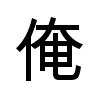
\includegraphics[scale=0.20]{images/ore.png}
	\end{center}
	The string \mintinline{java}{"\u4FFA\u306F\u6700\u9AD8\u3060\u305C\uFF01"}
	represents the phrase 
	\begin{center}
	
\includegraphics[scale=.30]{images/japanesePhraseHiRes}
	\end{center}
  \item Executable statements are terminated by a semicolon, \mintinline{java}{;}
  \item Code blocks are defined using opening and closing curly brackets, 
  	\mintinline{java}{{ ... }}.  Moreover, code blocks can be \emph{nested}: code
	blocks can be defined within other code blocks.  
  \item Variables are \glslink{scope}{scoped} to the code block in which they are declared
  	and are only valid within that code block.
  \item In general, whitespace between coding elements is ignored.
\end{itemize}

Though not a syntactic requirement, the proper use of whitespace is important for
good, readable code.  Code inside code blocks is indented at the same indentation.
Nested code blocks are indented further.  Think of a typical table of contents or
the outline of a formal paper or essay.  Sections and subsections or points and 
subpoints all follow proper indentation with elements at the same level at the same
indentation.  This convention is used to organize code and make it more readable.

\subsection{Program Structure}

\subsubsection{Classes}
\index{class}

In Java, everything is a \emph{class} or belongs to a class.  A class is an 
extensible program or blueprint for creating objects.  Objects are an integral
part of \gls{oopLabel} that we'll explore later.  However, to start out our
programs will be simple enough that the can be contained in a single class.
To declare a class, you use the following syntax.

\mintinline{java}{public class HelloWorld { ... }}

where the contents of the class are placed between the opening/closing curly
brackets.  In addition, a class must be placed in a Java source file with the same
name.  In our previous example, the class must be in a file named 
\mintinline{java}{HelloWorld.java}.  

When naming classes, the most commonly accepted naming convention 
is to use uppercase camel casing (also called PascalCase) in which each
word in the name is capitalized including the first, 
\mintinline{java}{Employee}, \mintinline{java}{SavingsAccount}, 
\mintinline{java}{ImageFile}, etc.  Class names (as well as their source file
names) are case sensitive.

\subsubsection{Packages}

Java code is organized into modules called \emph{packages}.  Packages
are essentially directories (or folders) which follow a directory tree 
structure which allows subdirectories and separate directories at the same
level.  It all starts at the \emph{root} directory called the ``default'' package.

Within a source file, we declare which package the file belongs to using
the keyword \mintinline{java}{package} followed by a \emph{fully qualified
package declaration} which is essentially just the names of the directories
that the file is located in, separated by a period.  The declaration is terminated
by a semicolon.  For example, the package declaration, 

\mintinline{java}{package unl.cse;}

would indicate that the file belongs in the directory \mintinline{java}{cse}
which is a subdirectory of the directory \mintinline{java}{unl}.  The
absence of a package declaration will mean that the file is associated
with the default directory.  

Packages allow you to organize source files and code functionality.  
Mathematics related classes can be placed in one package while 
image related classes can be placed in another, etc.  It also provides
separate name spaces for classes.  There could be 3 or 4 different
classes named \mintinline{java}{List} for example.  They could not
be located in the same directory; if you wanted to use one
which one would you be referring to?  By separating them into 
packages, they can all exist without conflict.  When we want to
use a particular one, we \emph{import} that class with its fully
qualified package name.

\subsubsection{Imports}

An \mintinline{java}{import} statement essentially ``brings in'' another
class so that its methods and functionality can be used.  For example, 
there is a class named \mintinline{java}{Scanner} (located in the
package \mintinline{java}{java.util}) that makes it easy to read input
from the standard input.  To include it in our program so that we can
use its functionality, we would need\footnote{You
can still use it without importing it, but you'd need to use a fully
qualified path name at declaration/instantiation.} to import it: 

\mintinline{java}{import java.util.Scanner;}

Classes in the package \mintinline{java}{java.lang} (such as 
\mintinline{java}{String} and \mintinline{java}{Math}) are 
considered standard and are imported by default without an 
explicit \mintinline{java}{import} statement.  

You may see some code that uses a \emph{wildcard} like
\mintinline{java}{import java.util.*;} which ends up importing
\emph{every} class in that package.  This is generally considered bad
practice.  In general, code should be intentional and specific, 
importing every class even if they are not used goes against
this principle. 

When naming packages, you must follow the general naming 
rules for identifiers (see below).  Package names cannot begin
with a number, no whitespace, etc.  Moreover, the general
convention for package names is to use lowercase underscore
casing, \mintinline{java}{here_is_an_example}.  Moreover, 
packages and subpackages follow the same convention as
directories: the top most directory is the most general and
subdirectories are more and more specific.  

In many of our examples we'll use \mintinline{java}{unl.cse} 
(UNL, University of Nebraska--Lincoln; CSE, Department of
Computer Science \& Engineering) which illustrates this 
general-to-specific organization.

There are many other important classes and packages provided by the
standard \gls{jdkLabel} that we'll examine as needed.  Of immediate
interest is the \mintinline{java}{Math} class and its library of
common mathematical functions such as the square root and the natural 
logarithm.  Table \ref{table:javaMathFunctions} highlights several of 
these functions.  To use them you'd need to invoke them by using the
class name and dot operator.  For example:

\begin{minted}{java}
double x = 1.5;
double y, z;
y = Math.sqrt(x); //y now has the value $\sqrt{x} = \sqrt{1.5}$
z = Math.sin(x); //z now has the value $\sin{(x)} = \sin{(1.5)}$
\end{minted}

In both of the method calls above, the value of the variable 
\mintinline{java}{x} is ``passed'' to the math function which computes 
and ``returns'' the result which then gets assigned to another variable.

\begin{table}
\centering
\begin{tabular}{l|l}
\hline
Function & Description \\
\hline
\mintinline{java}{Math.abs(x)}  & Absolute value function, $|x|$\textsuperscript{a}\\
\mintinline{java}{Math.ceil(x)} & Ceiling function, $\lceil 46.3\rceil = 47.0$\\
\mintinline{java}{Math.floor(x)} & Floor function, $\lfloor 46.3 \rfloor =46.0$\\
\\
\mintinline{java}{Math.cos(x)} & Cosine function\textsuperscript{b}\\
\mintinline{java}{Math.sin(x)} & Sine function\textsuperscript{b}\\
\mintinline{java}{Math.tan(x)} & Tangent function\textsuperscript{b}\\
\\
\mintinline{java}{Math.exp(x)} & Exponential function, $e^x$, $e = 2.71828\ldots$ \\
\mintinline{java}{Math.log(x)}  & Natural logarithm, $\ln{(x)}$\textsuperscript{c} \\
\mintinline{java}{Math.log10(x)} & Logarithm base 10, $\log_{10}{(x)}$\textsuperscript{c} \\
\\
\mintinline{java}{Math.pow(x,y)} & The power function, computes $x^y$\\
\mintinline{java}{Math.sqrt(x)} & Square root function\textsuperscript{c}\\

\hline
\end{tabular}
\caption[Several methods defined in the Java \mintinline{java}{Math} library]{Several methods defined in the Java \mintinline{java}{Math} library.  \textsuperscript{a}There are several versions of the absolute value method, 
one for each numeric type but all with the same name.  \textsuperscript{b}all trigonometric functions assume input is in \emph{radians}, \textbf{not} degrees. \textsuperscript{c}Input is assumed to be positive, $x > 0$.}
\label{table:javaMathFunctions}
\end{table}


\subsection{The \mintinline{java}{main()} Method}

Every executable program has to have a beginning: a point at which the
program starts to execute.  In Java, a class may contain many variables 
and methods, but a class is only \emph{executable} if it contains a 
\mintinline{java}{main()} method.  When a Java class is compiled and
the \gls{jvmLabel} is started, the JVM loads the class into memory and 
starts executing code contained in the \mintinline{java}{main()} method.

In addition, our \mintinline{java}{main()} method takes an \emph{array}
of \mintinline{java}{String} types which serve to communicate
any command line arguments provided to the program (review Section
\ref{subsection:commandLineInput} for details).  The array, 
\mintinline{java}{args} stores the arguments as strings.  The number
of arguments provided can be determined using the \mintinline{java}{length}
property of the array.  Specifically, \mintinline{java}{args.length} is
an integer indicating how many arguments were provided.  This does 
\emph{not} include the name of the program (class) itself as that is
already be known to the programmer.

To access any one argument, it will be necessary to
\emph{index} the array.  The index for the first argument is zero, thus the
first argument is \mintinline{java}{args[0]}, the second is \mintinline{java}{args[1]}, etc.
The last one would be at \mintinline{java}{args[args.length-1]}.

If a user is expected to provide numbers as input, they'll need to
be converted as the \mintinline{java}{args} array are only \mintinline{java}{String}
types.  To convert the arguments you can use parsing methods provided by the 
\mintinline{java}{Integer} and \mintinline{java}{Double} classes.
An example:

\begin{minted}{java}
//converts the "first" command line argument to an integer
int x = Integer.parseInt(args[0]);  
//converts the "third" command line argument to a double:
double y = Double.parseDouble(args[1]);
\end{minted}

\subsection{Comments}

Comments can be written in a Java program either as a single line using
two forward slashes, \mintinline{java}{//comment} or as a multiline comment using
a combination of forward slash and asterisk: \mintinline{java}{/* comment */}.  
With a single line comment, everything on the line \emph{after} the forward
slashes is ignored.  With a multiline comment, everything in between the forward
slash/asterisk is ignored.  Comments are ultimately ignored so
the amount of comments do not have an effect on the final executable code.
Consider the following example.

\begin{minted}{java}
//this is a single line comment
int x;  //this is also a single line comment, but after some code

/*
  This is a comment that can 
  span multiple lines to format the comment
  message more clearly
*/
double y;
\end{minted}

Most code editors and \glspl{ideLabel} will present comments in a special color or
font to distinguish them from the rest of the code (just as our example above does).
Failure to close a multiline comment will likely result in a compiler error but with
color-coded comments its easy to see the mistake visually.

Another common comment style convention is the Javadoc (Java Documentation)
style of comments.  Javadoc style comments are multiline comments that begin
with \mintinline{java}{/**}.  The Javadoc framework allows you
to \emph{markup} your comments with tags and links so that documentation can
be automatically generated and published.  We will sometimes use this style, but
we will not cover the details.  

\section{Variables}

Java has 8 built-in \gls{primitive} types supporting numbers (integers 
and floating point numbers), Booleans, and characters.  Table \ref{table:javaPrimitives}
contains a complete description of these types.  Each of these primitive
types also has a corresponding \emph{wrapper} class defined in the 
\mintinline{java}{java.lang} package.  Wrapper classes provide \emph{object}
versions of each of these classes.  The object versions have many utility
methods that can be used in relation to their type.  For example, the
aforementioned \mintinline{java}{Integer.parseInt()} method is part of the 
\mintinline{java}{Integer} wrapper class.

\begin{table}
\centering
\begin{tabular}{l|l|l}
 Type & Description & Wrapper Class\\
\hline\hline
\mintinline{java}{byte} & 8-bit signed 2s complement integer & \mintinline{java}{Byte} \\
\mintinline{java}{short} & 16-bit signed 2s complement integer  & \mintinline{java}{Short} \\
\mintinline{java}{int} & 32-bit signed 2s complement integer & \mintinline{java}{Integer}  \\
\mintinline{java}{long} & 64-bit signed 2s complement integer  & \mintinline{java}{Long} \\
\mintinline{java}{float} & 32-bit IEEE 754 floating point number & \mintinline{java}{Float} \\
\mintinline{java}{double} & 64-bit floating point number & \mintinline{java}{Double}  \\
\mintinline{java}{boolean} & may be set to \mintinline{java}{true} or \mintinline{java}{false} & \mintinline{java}{Boolean} \\
\mintinline{java}{char} & 16-bit Unicode (UTF-16) character & \mintinline{java}{Character}  \\
\end{tabular}
\caption{Primitive types in Java}
\label{table:javaPrimitives}
\end{table}

The wrapper classes, however, are different.  These are objects, so when a reference is declared
for them, by default, that reference refers to \mintinline{java}{null}.  The keyword \mintinline{java}{null}
is used to indicate a special memory address that represents ``nothing.''  In fact, the
default value for \emph{any} object type is \mintinline{java}{null}.  Care must be taken
when mixing primitive types and their wrapper classes (see below) as \mintinline{java}{null}
references may result in a \mintinline{java}{NullPointerException}.  Finally, instances
of the wrapper classes are \gls{immutable}.  Once they are created, they cannot be changed.
References can be made to refer to a different object, but the object's value cannot
be changed.  

\subsection{Declaration \& Assignment}

Java is a statically typed language meaning that all variables must be declared
before you can use them or refer to them.  In addition, when declaring a variable, 
you must specify both its type and its identifier.  For example:

\begin{minted}{c}
int numUnits;
double costPerUnit;
char firstInitial;
boolean isStudent;
\end{minted}

Each declaration specifies the variable's type followed by the 
identifier and ending with a semicolon.  The identifier rules are 
fairly standard: a name can consist of lowercase and uppercase 
alphabetic characters, numbers, and underscores but may 
\emph{not} begin with a numeric character.  We adopt the 
modern camelCasing naming convention for variables in our 
code.  In general, variables \emph{must} be assigned a value before
you can use them
in an expression.  You do not have to immediately assign a value
when you declare them (though it is good practice), but some value
must be assigned before they can be used or the compiler
will issue an error.\footnote{Instance variables, that is variables
declared as part of an object \emph{do} have default values.
For objects, the default is \mintinline{java}{null}, for all numeric 
types, zero is the default value.  For the \mintinline{java}{boolean} 
type, \mintinline{java}{false} is the default, and the default 
\mintinline{java}{char} value is \mintinline{text}{\0}, the 
null-terminating character (zero in the \gls{asciiLabel} table).}

The assignment operator is a single equal sign, \mintinline{java}{=} and is a right-to-left
assignment.  That is, the variable that we wish to assign the value to appears on the
left-hand-side while the value (literal, variable or expression) is on the right-hand-size.
Using our variables from before, we can assign them values:

\begin{minted}{java}
numUnits = 42;
costPerUnit = 32.79;
firstInitial = 'C';
isStudent = true;
\end{minted}

For brevity, Java allows you to declare a variable and immediately assign 
it a value on the same line.  So these two code blocks could have been 
more compactly written as:

\begin{minted}{c}
int numUnits = 42;
double costPerUnit = 32.79;
char firstInitial = 'C';
boolean isStudent = true;
\end{minted}

As another shorthand, we can declare multiple variables on the same line by delimiting
them with a comma.  However, they \emph{must} be of the same type.  We can also 
use an assignment with them. 

\begin{minted}{c}
int numOrders, numUnits = 42, numCustomers = 10, numItems;
double costPerUnit = 32.79, salesTaxRate;
\end{minted}

Another useful keyword is \mintinline{java}{final}.  Though it has several uses, 
when applied to a variable declaration, it makes it a read-only variable.  After a
value has been assigned to a \mintinline{java}{final} variable, its value cannot
be changed.  

\begin{minted}{java}
final int secret = 42;
final double salesTaxRate = 0.075;
\end{minted}

Any attempt to reassign the values of \mintinline{java}{final} variables will result
in a compiler error.

\section{Operators}

Java supports the standard arithmetic operators for addition, subtraction, multiplication, and
division using \mintinline{java}{+}, \mintinline{java}{-}, \mintinline{java}{*}, and
\mintinline{java}{/} respectively.  Each of these operators is a binary operator that
acts on two operands which can either be literals or other variables and follow
the usual rules of arithmetic when it comes to order of precedence (multiplication 
and division before addition and subtraction).

\begin{minted}{java}
int a = 10, b = 20, c = 30, d;
d = a + 5;
d = a + b;
d = a - b;
d = a + b * c;
d = a * b;
d = a / b; //integer division and truncation!  See below

double x = 1.5, y = 3.4, z = 10.5, w;
w = x + 5.0;
w = x + y;
w = x - y;
w = x + y * z;
w = x * y;
w = x / y;

//you can do arithmetic with both types:
w = a + x;

//however you CANNOT assign a double to an integer:
d = b + y; //compilation error
//but you can do so with an explicit type cast:
d = (int) (b + y);  //though truncation occurs, d is 23
\end{minted}

In addition, you can \emph{mix} the wrapper classes with their primitive types.
You must be careful though.  The wrapper classes are object references which
can be \mintinline{java}{null}.  If a \mintinline{java}{null} reference is used
in an arithmetic expression, it will result in a \mintinline{java}{NullPointerException}
which can be caught and handled (see Chapter \ref{chapter:java:errorHandling}).  
If not caught, it will end up being a fatal
error.  Some examples:

\begin{minted}{java}
int a = 10, c;
Integer b = 20;

//int and Integer can be mixed:
c = a + b;

double x = 3.14, z;
Double y = 2.71;
//double and Double can be mixed:
z = x + y;

//all types can be mixed:
double u = a + x + b + y;

//Be careful:
Integer d = null;
c = a + d; //NullPointerException
\end{minted}

This works because of a mechanism called \emph{autoboxing} (or \emph{autounboxing} in
this case).  The wrapper class is acting like a ``box'': it is an object that stores
the value of a primitive type.  When it gets used in an arithmetic expression, it
gets ``unboxed'' and converted to a primitive type so that the arithmetic
operation is performed on compatible primitive types.  This is all done by the 
compiler and is completely transparent to us.  However, that is the reason that
we may get a \mintinline{java}{NullPointerExcpetion}.  Our code actually gets
converted from \mintinline{java}{c = a + d;} to \mintinline{java}{c = a +d.doubleValue();}.
The \mintinline{java}{doubleValue()} method returns a \mintinline{java}{double} primitive
value.  However, if \mintinline{java}{d} is \mintinline{java}{null}, you can't call
a method on it; thus the \mintinline{java}{NullPointerException} is thrown
as a consequence.

Special care must be taken when dealing with \mintinline{java}{int} types.  
For all four operators, if both operands are integers, the result will be an
integer.  For addition, subtraction, and multiplication this isn't an issue, but
for division it means that when we divide, say \mintinline{java}{(10 / 20)}, the result
is not $0.5$ as expected.  The number 0.5 is a floating point number.  As
such, the fractional part gets \glslink{truncation}{truncated} (cut off and thrown out) leaving
only zero.  In the code above, \mintinline{java}{d = a / b;} the variable \mintinline{java}{d}
ends up getting the value zero because of this.

A solution to this problem is to use explicit \gls{type casting} to force at
least one of the operands in an integer division to become a \mintinline{java}{double}
type.  For example:

\begin{minted}{java}
int a = 10, b = 20;
double x;

x = (double) a / b; 
\end{minted}

Assigning a floating point number to an integer is not allowed in
Java and attempting to do so will be treated as a compiler error.  This
is because Java does not support \emph{implicit} type casts.
However, you \emph{can} do so if you provide an \emph{explicit} type cast
as in the code above, 

\mintinline{java}{d = (int) (b + y);}

In this code, \mintinline{java}{b + y} is correctly computed as $20 + 3.4 = 23.4$, 
but the explicit type cast (down to an integer) results in truncation.  The $.4$ 
gets cutoff and \mintinline{java}{d} gets the value 23. Assigning an 
\mintinline{java}{int} value to a \mintinline{java}{double} variable is
not a problem as the integer $2$ becomes the floating point number $2.0$.

Java also supports the integer remainder operator using the \mintinline{java}{%} symbol.
This operator gives the remainder of the result of dividing two integers.  Examples:

\begin{minted}{java}
int x;

x = 10 % 5; //x is 0
x = 10 % 3; //x is 1
x = 29 % 5; //x is 4
\end{minted}

\section{Basic I/O}

Java provides several ways to perform input and output operations 
with the standard
input/output as part of the \mintinline{java}{System} class.  The \mintinline{java}{System}
class contains a standard output stream which can be accessed using \mintinline{java}{System.out}.
It also has a standard input stream which can be accessed using \mintinline{java}{System.in}.

For output, there are several methods that can be used but we'll focus on \mintinline{java}{System.out.println()}
and \mintinline{java}{System.out.printf()}.  The first is for printing strings on a single line.  The \mintinline{java}{ln}
at the end indicates that the method will insert an endline character, \mintinline{text}{\n} for you.
The second is a \mintinline{java}{printf}-style output method that takes placeholders like \mintinline{java}{%d} 
and \mintinline{java}{%f} (review Section \ref{subsection:printfStyleFormatting} for details).

The easiest way to read input is through the \mintinline{java}{Scanner} class.  You can create
a new instance of the \mintinline{java}{Scanner} class and associate it with the standard input using the following
code.

\mintinline{java}{Scanner s = new Scanner(System.in);}

The variable \mintinline{java}{s} is now active and can be read from.  You can get specific
values from the \mintinline{java}{Scanner} by calling various methods such as \mintinline{java}{s.nextInt()}
to get an \mintinline{java}{int}, \mintinline{java}{s.nextDouble()} to get a \mintinline{java}{double}, etc.
When these methods are called, the program \emph{blocks} until the user enters her input
and presses the enter/return key.  The conversion to the type you requested is automatic.
A full example is depicted in Code Sample \ref{code:java:basicIO}.

\begin{listing}
\begin{minted}{java}
Scanner s = new Scanner(System.in);
int a;
System.out.println("Please enter a number: ");
a = s.nextInt();
System.out.printf("Great, you entered %d\n", a);
\end{minted}
\caption{Basic Input/Output in Java}
\label{code:java:basicIO}
\end{listing}

One potential problem with using \mintinline{java}{Scanner} is that the 
methods cannot force a user to enter good input.  In the example above,
if the user, instead of entering a number, entered \mintinline{java}{"Hello"}, 
the conversion to a number would fail and result in a 
\mintinline{java}{InputMismatchException}.

\section{Examples}

\subsection{Converting Units}

Let's write a program that will prompt 
the user to enter a temperature in degrees Fahrenheit and convert 
it to degrees Celsius using the formula
  $$C = (F - 32) \cdot \frac{5}{9}$$

We begin with the basic program outline which will include a package and
class declaration.  We'll also need
to read from the standard input, so we'll import the \mintinline{java}{Scanner}
class.  We'll want want our class to be executable, so we need to 
put a \mintinline{java}{main()} method in our class.  Finally, we'll document
our program to indicate its purpose.


\begin{minted}{java}
package unl.cse;

import java.util.Scanner;

/**
 * This program converts Fahrenheit temperatures to 
 * Celsius
 */
public class TemperatureConverter {

  public static void main(String args[]) {

    //TODO: implement this

  }
}
\end{minted}

It is common for programmers to use a comment along with a 
\mintinline{java}{TODO} note to themselves as a reminder of things 
that they still need to do with the program.  

Let's first outline the basic steps that our program will go through:
\begin{enumerate}
  \item We'll first prompt the user for input, asking them for a temperature in Fahrenheit
  \item Next we'll read the user's input, likely into a floating point number as degrees can be fractional
  \item Once we have the input, we can calculate the degrees Celsius by using the formula above
  \item Lastly, we will want to print the result to the user to inform them of the value
\end{enumerate}
Sometimes it is helpful to write an outline of such a program directly in the code using
comments to provide a step-by-step process.  For example:

\begin{minted}{java}
package unl.cse;

import java.util.Scanner;

/**
 * This program converts Fahrenheit temperatures to 
 * Celsius
 */
public class TemperatureConverter {

  public static void main(String args[]) {

    //TODO: implement this
    //1. Prompt the user for input in Fahrenheit
    //2. Read the Fahrenheit value from the standard input
    //3. Compute the degrees Celsius
    //4. Print the result to the user

  }
}
\end{minted}

As we read each step it becomes apparent that we'll need a couple of variables:
one to hold the Fahrenheit (input) value and one for the Celsius (output) value.  It also
makes sense that each of these should be \mintinline{java}{double} variables as we
want to support fractional values.  At the top of our \mintinline{java}{main()} method, 
we'll add the variable declarations:

\mintinline{java}{double fahrenheit, celsius;}

We'll also need a \mintinline{java}{Scanner}, initialized to read from the standard input: 

\mintinline{java}{Scanner s = new Scanner(System.in);}

Each of the steps is now straightforward; we'll use a \mintinline{java}{System.out.println()} statement in the
first step to prompt the user for input:

\mintinline{java}{System.out.println("Please enter degrees in Fahrenheit: ");}

In the second step, we'll use our \mintinline{java}{Scanner} to read in
a value from the user for the \mintinline{java}{fahrenheit} variable.  
Recall that we use the method \mintinline{java}{s.nextDouble()} to
read a \mintinline{java}{double} value from the user.

\mintinline{java}{fahrenheit = s.nextDouble();}

We can now compute \mintinline{java}{celsius} using the formula provided:

\mintinline{java}{celsius = (fahrenheit - 32) * (5 / 9);}

Finally, we use \mintinline{java}{System.out.printf()} to output the result to the user:

\mintinline{java}{System.out.printf("%f Fahrenheit is %f Celsius\n", fahrenheit, celsius);}  

Try typing and running the program as defined above and you'll find that
you don't get correct answers.  In fact, you'll find that no matter what
values you enter, you get zero.  This is because of the calculation using
\mintinline{java}{(5 / 9)}: recall what happens with integer division: truncation! 
This will \emph{always} end up being zero.  

One way we could fix it would be to pull out our calculators and find that
$\frac{5}{9} = 0.55555\ldots$ and replace \mintinline{java}{(5 / 9)} with \mintinline{java}{0.555555}.
But, how many fives?  It may be difficult to tell how accurate we can make
this floating point number by hardcoding it ourselves.  A much better approach
would be to let the compiler take care of the optimal computation for us by
making at least one of the numbers a \mintinline{java}{double} to prevent
integer truncation.  That is, we should instead use \mintinline{java}{5.0 / 9}.
The full program can be found in Code Sample \ref{code:java:fahrenheitToCelsiusProgram}.

\begin{listing}[H]
\begin{minted}{java}
package unl.cse;

import java.util.Scanner;

public class TemperatureConverter {

  public static void main(String args[]) {

    double fahrenheit, celsius;
    Scanner s = new Scanner(System.in);

    //1. Prompt the user for input in Fahrenheit
    System.out.println("Please enter degrees in Fahrenheit: ");
      
    //2. Read the Fahrenheit value from the standard input
    fahrenheit = s.nextDouble();
      
    //3. Compute the degrees Celsius
    celsius = (fahrenheit - 32) * 5.0 / 9;
      
    //4. Print the result to the user
    System.out.printf("%f Fahrenheit is %f Celsius\n", 
    	fahrenheit, celsius);

  }
}
\end{minted}
\caption{Fahrenheit-to-Celsius Conversion Program in Java}
\label{code:java:fahrenheitToCelsiusProgram}
\end{listing}

\subsection{Computing Quadratic Roots}

Some programs require the user to enter multiple inputs.  The 
prompt-input process can be repeated.  In this example, consider asking
the user for the coefficients, $a, b, c$ to a quadratic polynomial, 
  $$ax^2 + bx + c$$
and computing its roots using the quadratic formula, 
  $$x = \frac{-b \pm \sqrt{b^2 - 4ac}}{2a}$$
As before, we can create a basic program with a \mintinline{java}{main()}
method and start filling in the details.  In particular, we'll need to prompt
for the input $a$, then read it in; then prompt for $b$, read it in and
repeat for $c$.  We'll also need several variables: three for the coefficients
$a, b, c$ and \emph{two} more; one for each root. 

\begin{minted}{java}
    double a, b, c, root1, root2;
    Scanner s = new Scanner(System.in);

    System.out.println("Please enter a: ");
    a = s.nextDouble();
    System.out.println("Please enter b: ");
    b = s.nextDouble();
    System.out.println("Please enter c: ");
    c = s.nextDouble();
\end{minted}

Now to compute the roots: we need to adapt the
formula so it accurately reflects the order of operations.  We also need to use
the standard math library's square root method.

\begin{minted}{java}
root1 = (-b + Math.sqrt(b*b - 4*a*c) ) / (2*a);
root2 = (-b - Math.sqrt(b*b - 4*a*c) ) / (2*a);
\end{minted}

Finally, we print the output using \mintinline{java}{System.out.printf()}.  The full program 
can be found in Code Sample \ref{code:java:quadraticRootsProgram}.

\begin{listing}[h]
\begin{minted}{java}
package unl.cse;

import java.util.Scanner;

/**
 * This program computes the roots to a quadratic equation
 * using the quadratic formula.
 */
public class QuadraticRoots {

  public static void main(String args[]) {
	  
    double a, b, c, root1, root2;
    Scanner s = new Scanner(System.in);

    System.out.println("Please enter a: ");
    a = s.nextDouble();
    System.out.println("Please enter b: ");
    b = s.nextDouble();
    System.out.println("Please enter c: ");
    c = s.nextDouble();
	  
    root1 = (-b + Math.sqrt(b*b - 4*a*c) ) / (2*a);
    root2 = (-b - Math.sqrt(b*b - 4*a*c) ) / (2*a);
	  
    System.out.printf("The roots of %fx^2 + %fx + %f are: \n", 
    	a, b, c);
    System.out.printf("  root1 = %f\n", root1);
    System.out.printf("  root2 = %f\n", root2);

  }

}
\end{minted}
\caption{Quadratic Roots Program in Java}
\label{code:java:quadraticRootsProgram}
\end{listing}

This program was interactive.  As an alternative, we could have read 
all three of the inputs as command line arguments, taking care that we
need to convert them to floating point numbers.  Lines 16--21 in the
program could have been changed to 

\begin{minted}{java}
a = Double.parseDouble(args[0]);
b = Double.parseDouble(args[1]);
c = Double.parseDouble(args[2]);
\end{minted}

Finally, think about the possible inputs a user could provide that may cause problems
for this program.  For example:
\begin{itemize}
  \item What if the user entered zero for $a$?
  \item What if the user entered some combination such that $b^2 < 4ac$?
  \item What if the user entered non-numeric values?
  \item For the command line argument version, what if the user provided less than
  	three arguments?  Or more?
\end{itemize}
How might we prevent the consequences of such bad input?  
How might we handle the event that a user enters bad input and
how do we communicate these errors to the user?  To start to resolve
these issues, we'll need conditionals.


\chapter{Conditionals}
%!TEX root = ComputerScienceOne.tex

%%Chapter: Java Conditionals
\index{conditionals!in Java}
\index{Java!conditionals}

Java supports the basic if, if-else, and if-else-if conditional structures as well as switch
statements.  Java has Boolean types and logical statements are built using the standard 
logical operators for numeric comparisons as well as logical operators such as negations, 
\And, and \Or\ that can be used with Boolean types.

\section{Logical Operators}

Recall that Java has Boolean types built-in to the language using
either the primitive type, \mintinline{java}{boolean} or its wrapper class
\mintinline{java}{Boolean}.  Moreover, the keywords \mintinline{java}{true}
and \mintinline{java}{false} can be used to assign and check values.
Because Java has Boolean types, it does not allow you to mix logical operators
with numeric types.  That is, code like the following is invalid.

\begin{minted}{java}
int a = 10;
boolean b = true;
boolean result = (a || b); //compilation error
\end{minted}

The standard numeric comparison operators are also supported.  Consider the 
following code snippet:

\begin{minted}{java}
int a = 10;
int b = 20;
int c = 10;
boolean x = true;
boolean y = false;
\end{minted}

The six standard comparison operators are presented in Table \ref{table:java:comparisonOperators}
using these variables as examples.  The comparison operators are the same when
used with \mintinline{java}{double} types as well and \mintinline{java}{int} types and can be compared with each other without type casting.

\begin{table}
\centering
\begin{tabular}{l|l|l|l}
Name & Operator Syntax & Examples  & Value \\
\hline\hline
Equals & \mintinline{java}{==} & 
	\mintinline{java}{a == 10} & \True \\
~ & ~ & \mintinline{java}{b == 10} & \False \\
~ & ~ & \mintinline{java}{a == b} & \False \\
~ & ~ & \mintinline{java}{a == c} & \True \\
\hline	
Not Equals & \mintinline{java}{!=} & 
	\mintinline{java}{a != 10} & \False \\
~ & ~ & \mintinline{java}{b != 10} & \True \\
~ & ~ & \mintinline{java}{a != b} & \True \\
~ & ~ & \mintinline{java}{a != c} & \False \\
\hline	
Strictly Less Than & \mintinline{java}{<} & 
	\mintinline{java}{a < 15} & \True \\
~ & ~ & \mintinline{java}{a < 5} & \False \\
~ & ~ & \mintinline{java}{a < b} & \True \\
~ & ~ & \mintinline{java}{a < c} & \False \\
\hline
Less Than Or Equal To & \mintinline{java}{<=} & 
	\mintinline{java}{a <= 15} & \True \\
~ & ~ & \mintinline{java}{a <= 5} & \False \\
~ & ~ & \mintinline{java}{a <= b} & \True \\
~ & ~ & \mintinline{java}{a <= c} & \True \\
\hline
Strictly Greater Than & \mintinline{java}{>} & 
	\mintinline{java}{a > 15} & \False \\
~ & ~ & \mintinline{java}{a > 5} & \True \\
~ & ~ & \mintinline{java}{a > b} & \False \\
~ & ~ & \mintinline{java}{a > c} & \False \\
\hline
Greater Than Or Equal To & \mintinline{java}{>=} & 
	\mintinline{java}{a >= 15} & \False \\
~ & ~ & \mintinline{java}{a >= 5} & \True \\
~ & ~ & \mintinline{java}{a >= b} & \False \\
~ & ~ & \mintinline{java}{a >= c} & \True \\
\hline	
\end{tabular}
\caption{Comparison Operators in Java}
\label{table:java:comparisonOperators}
\end{table}

Furthermore, because of autoboxing and unboxing, the wrapper classes for 
numeric types can be compared using the same operators.  For example:

\begin{minted}{java}
int a = 10;
Integer b = 20;
Double x = 3.14;
boolean r;
r = (a < b);
r = (a >= b);
r = (x == 2.71);
\end{minted}

The three basic logical operators are also supported as described in 
Table \ref{table:java:logicOperators}.

\begin{table}
\centering
\begin{tabular}{l|l|l|l}
Operator & Operator Syntax & Examples & Values \\
\hline\hline
Negation & \mintinline{java}{!} & 
	\mintinline{java}{!x} & \False \\
~ & ~ & \mintinline{java}{!y} & \True \\
\hline
\And & \mintinline{java}{&&} & 
	\mintinline{java}{x && true} & \True \\
~ & ~ & \mintinline{java}{x && y} & \False \\
\hline
\Or & \mintinline{java}{||} & 
	\mintinline{java}{x || false} & \True \\
~ & ~ & \mintinline{java}{x || y} & \True \\
~ & ~ & \mintinline{java}{!x || y} & \False \\
\end{tabular}
\caption{Logical Operators in Java with \mintinline{java}{x = true}
and \mintinline{java}{y = false} both being \mintinline{java}{Boolean}
variables.}
\label{table:java:logicOperators}
\end{table}

\subsection{Order of Precedence}

At this point it is worth summarizing the order of precedence of all the 
operators that we've seen so far including assignment, arithmetic, 
comparison, and logical.  Since all of these operators could be used
in one statement, for example, 

\mintinline{java}{(b*b < 4*a*c || a == 0 || args.length != 4)}

It is important to understand the order in which each one gets evaluated.
Table \ref{table:java:operatorPrecedence} summarizes the order of precedence
for the operators seen so far.  This is not an exhaustive list of Java operators.

\begin{table}
\centering
\begin{tabular}{l|l|l|p{6cm}}
~ & Operator(s) & Associativity & Notes \\
\hline\hline
Highest & \mintinline{java}{++}, \mintinline{java}{--} & left-to-right & postfix increment operators\\
~ & \mintinline{java}{-},  \mintinline{java}{!} & right-to-left & unary negation operator, logical not\\
~ & \mintinline{java}{*},  \mintinline{java}{/}, \mintinline{java}{%} & left-to-right & ~\\
~ & \mintinline{java}{+},  \mintinline{java}{-} & left-to-right & addition, subtraction\\
~ & \mintinline{java}{<},  \mintinline{java}{<=}, \mintinline{java}{>}, \mintinline{java}{>=} & left-to-right & comparison \\
~ & \mintinline{java}{==},  \mintinline{java}{!=} & left-to-right & equality, inequality \\
~ & \mintinline{java}{&&} & left-to-right & logical \And \\
~ & \mintinline{java}{||}  & left-to-right & logical \Or \\
Lowest & \mintinline{java}{=}, \mintinline{java}{+=}, \mintinline{java}{-=}, \mintinline{java}{*=}, \mintinline{java}{/=}  & right-to-left & assignment and compound assignment operators \\
\end{tabular}
\caption[Operator Order of Precedence in Java]{Operator Order of Precedence in Java.
Operators on the same level have equivalent order and are performed in the associative
order specified.}
\label{table:java:operatorPrecedence}
\end{table}

\subsection{Comparing Strings and Characters}

The comparison operators in Table \ref{table:java:comparisonOperators} can also be used
for \emph{single characters} because of the nature of the ASCII text table (see Table \ref{table:asciiTable}).
Each alphanumeric character, including the various symbols and whitespace characters, 
is associated with an integer 0--127.  We can therefore write statements like \mintinline{java}{('A' < 'a')}, 
which is \True since uppercase letters are ordered before lowercase letters in the ASCII
table (\mintinline{java}{'A'} is 65 and \mintinline{java}{'a'} is 97 and so $65 < 97$ is \True).
Several more examples can be found in Table \ref{table:java:asciiComparisonExamples}.

\begin{table}[h]
\centering
\begin{tabular}{c|l}
Comparison Example & Result \\
\hline\hline
\mintinline{java}{('A' < 'a')} & \True \\ 
\mintinline{java}{('A' == 'a')} & \False \\ 
\mintinline{java}{('A' < 'Z')} & \True \\ 
\mintinline{java}{('0' < '9')} & \True \\ 
\mintinline{java}{('\n' < 'A')} & \True \\ 
\mintinline{java}{(' ' < '\n')} & \False \\ 
\end{tabular}
\caption{Character comparisons in Java}
\label{table:java:asciiComparisonExamples}
\end{table}

Numeric comparison operators \emph{cannot} be used to compare strings in Java.  For example,
we could \emph{not} code something like \mintinline{java}{("aardvark" < "zebra")}.  The Java
compiler would not allow you to do this because the comparison operator is for numeric types 
\emph{only}.  However, the following code \emph{would} compile and run:

\begin{minted}{java}
String s = "aardvark";
String t = "zebra";
boolean b = (s == t);
\end{minted}

but it wouldn't necessarily give you what you want.  To understand why this is okay, recall that
a \mintinline{java}{String} is an object; the \mintinline{java}{s} and \mintinline{java}{t} variables
are \emph{references} to that object in memory.  When we use the equality comparison, \mintinline{java}{==}
we're asking if \mintinline{java}{s} and \mintinline{java}{t} are the \emph{same memory address}.
In this case, likely they are not and so the result is \mintinline{java}{false}.  However, similar code, 

\begin{minted}{java}
String s = new String("liger");
String t = new String("liger");
boolean b = (s == t);
\end{minted}

would also result in \mintinline{java}{false} because \mintinline{java}{s} and \mintinline{java}{t} represent
different strings in memory, even though they have the same sequence of characters.
We'll explore how to properly compare strings later.  For now, avoid using the
equality operators with strings.

\section{If, If-Else, If-Else-If Statements}

Conditional statements in Java utilize the keywords \mintinline{java}{if}, \mintinline{java}{else}, and
\mintinline{java}{else if}.  Conditions are placed inside parentheses immediately after the 
\mintinline{java}{if} and \mintinline{java}{else if} keywords.  Examples of all three can be 
found in Code Sample \ref{code:java:conditionalExamples}.

\begin{listing}
\begin{minted}{java}
//example of an if statement:
if(x < 10) {
  System.out.println("x is less than 10");
}

//example of an if-else statement:
if(x < 10) {
  System.out.println("x is less than 10");
} else {
  System.out.println("x is 10 or more");
}

//example of an if-else-if statement:
if(x < 10) {
  System.out.println("x is less than 10");
} else if(x == 10) {
  System.out.println("x is equal to ten");
} else {
  System.out.println("x is greater than 10");
}
\end{minted}
\caption{Examples of Conditional Statements in Java}
\label{code:java:conditionalExamples}
\end{listing}

The statement, \mintinline{java}{if(x < 10)}
does not have a semicolon at the end.  This is because it is a conditional statement
that determines the flow of control and \emph{not} an executable statement.  
Therefore, no semicolon is used.  Suppose we made a mistake and \emph{did}
include a semicolon:

\begin{minted}{java}
int x = 15;
if(x < 10); {
  System.out.println("x is less than 10");
}
\end{minted}

Some compilers may give a warning, but this is valid Java; it will compile and it 
will run.  However, it will end up printing \mintinline{java}{x is less than 10}, even
though $x = 15$!  Recall that a conditional statement \emph{binds} to the 
executable statement or code block \emph{immediately} following it.  In this
case, we've provided an \emph{empty} executable statement ended by the
semicolon.  The code is essentially equivalent to 

\begin{minted}{java}
int x = 15;
if(x < 10) {
}
System.out.println("x is less than 10");
\end{minted}

Which is obviously not what we wanted.  The semicolon ended up binding 
to the empty executable statement, and the code block containing the
print statement immediately followed, but was \emph{not} bound to the
conditional statement which is why the print statement executed regardless
of the value of $x$.

Another convention that we've used in our code is where we have placed the
curly brackets.  First, if a conditional statement is bound to only one statement, 
the curly brackets are not necessary.  However, it is best practice to include them
even if they are not necessary and we'll follow this convention.  Second, the
opening curly bracket is on the same line as the conditional statement while
the closing curly bracket is indented to the same level as the start of the
conditional statement.  Moreover, the code inside the code block is indented.
If there were more statements in the block, they would have all been at the
same indentation level.

%\section{Switch statements}
%
%TODO: should we actually do this?
%
%C also supports switch statements, but only for integer types.  The usual
%syntax applies as do the fall-through rules.  Switch statements also work 
%on \mintinline{java}{char} types since in C, they can be treated as integers
%according to the ASCII text table.
%
%\begin{listing}[H]
%\begin{minted}{c}
%int x;
%...
%switch(x) {
%  case 0: 
%    printf("x is zero\n");
%    break;
%  case 1:
%  case 2:
%    printf("x is one or 2\n");
%    break;
%  case 3:
%    printf("x is 3\n");
%    break;
%  case 10:
%    printf("x is 10\n");
%    break;
%  default:
%    printf("x is not 0, 1, 2, 3, nor 10\n");
%    break;
%}
%\end{minted}
%\caption{Switch Statement in C}
%\label{code:c:switchStatement}
%\end{listing}
%
%TODO: more here?

\section{Examples}

\subsection{Computing a Logarithm}

The logarithm of $x$ is the exponent that some \emph{base} must 
be raised to get $x$.  The most common logarithm is the natural logarithm, 
$\ln{(x)}$ which is base $e = 2.71828\ldots$.  But logarithms can be in any base 
$b > 1$.\footnote{Bases can also be $0< b < 1$, but we'll restrict our attention to
increasing functions only.}  What if we wanted to compute $\log_2{(x)}$?  
Or $\log_{\pi}{(x)}$?  Let's write a program that will prompt the user for a
number $x$ and a base $b$ and computes $\log_b{(x)}$.

Arbitrary bases can be computed using the change of base formula: 
  $$\log_b(x) = \frac{\log_a{(x)}}{\log_a{(b)}}$$
If we can compute \emph{some} base $a$, then we can compute any base 
$b$.  Fortunately we have such a solution.  Recall that the standard library 
provides a function to compute the natural logarithm, \mintinline{java}{Math.log()}.
This is one of the fundamentals of problems solving: if a solution already 
exists, use it.  In this case, a solution exists for a different, but similar problem
(computing the natural logarithm), but we can \emph{adapt} the solution 
using the change of base formula.  In particular, if we have variables 
\mintinline{java}{b} (base) and \mintinline{java}{x}, we can compute $\log_b{(x)}$ using

  \mintinline{java}{Math.log(x) / Math.log(b)}
  
However, we have a problem similar to the examples in the previous section.  
The user could enter invalid values such as $b = -10$ or $x = -2.54$ 
(logarithms are undefined for non-positive values in any base).  We want
to ensure that $b > 1$ and $x > 0$.  With conditionals, we can now do this.  
Once we have read in the input from the user we can make a check for
good input using an \mintinline{java}{if} statement.

\begin{minted}{java}
if(x <= 0 || b <= 1) {
  System.out.println("Error: bad input!");
  System.exit(1);
}
\end{minted}

This code has something new: \mintinline{java}{System.exit(1)}.  The \mintinline{java}{exit()}
function immediately terminates the program regardless of the rest of the
code that it may remain.  The argument passed to \mintinline{java}{exit()} is an 
integer that represents an \emph{error code}.  The convention is that 
zero indicates ``no error'' while non-zero values indicate some error.  This
is a simple way of performing \emph{error handling}: if the user provides
bad input, we inform them and quit the program, forcing them to run it
again and provide good input.  By prematurely terminating the program
we avoid any illegal operation that would give a bad result.

Alternatively, we could have split the conditions into two statements and given
a more descriptive error message.  We use this design in the full program 
which can be found in Code Sample \ref{code:java:logarithmProgram}.  The 
program also takes the input as command line arguments.  Now that we have
conditionals, we can actually check that the correct number of arguments
was provided by the user and quit in the event that they don't provide
the correct number.

\begin{listing}[h]
\begin{minted}{java}
/**
 * This program computes the logarithm base b (b > 1) 
 * of a given number x > 0
 */
public class Logarithm {

  public static void main(String args[]) {

    double b, x, result;
    if(args.length != 2) {
      System.out.println("Usage: b x");
      System.exit(1);
    }  
	  
    b = Double.parseDouble(args[0]);
    x = Integer.parseInt(args[1]);

    if(x <= 0) {
      System.out.println("Error: x must be greater than zero");
      System.exit(1);
    }
    if(b <= 1) {
      System.out.println("Error: base must be greater than one");
      System.exit(1);
    }

    result = Math.log(x) / Math.log(b);
    System.out.printf("log_(%f)(%f) = %f\n", b, x, result);

  }

}
\end{minted}
\caption{Logarithm Calculator Program in Java}
\label{code:java:logarithmProgram}
\end{listing}

\subsection{Life \& Taxes}

Let's adapt the conditional statements we developed in Section \ref{subsubsection:lifeAndTaxes}
into a full Java program.  The first thing we need to do is establish the variables we'll need and
read them in from the user.  At the same time we can check for bad input (negative values)
for both the inputs.

\begin{minted}{java}
Scanner s = new Scanner(System.in);
double income, baseTax, numChildren, credit, totalTax;

System.out.println("Please enter your Adjusted Gross Income: ");
income = s.nextDouble();

System.out.println("How many children do you have?");
numChildren = s.nextDouble();

if(income < 0 || numChildren < 0) {
  System.out.println("Invalid inputs");   
  System.exit(1);
}
\end{minted}

Next, we can code a series of if-else-if statements for the income range.  By
placing the ranges in increasing order, we only need to check the upper bounds
just as in the original example.

\begin{minted}{java}
  if(income <= 18150) {
    baseTax = income * .10;
  } else if(income <= 73800) {
    baseTax = 1815 + (income - 18150) * .15;
  } else if(income <= 148850) {
  ...  
  } else {
    baseTax = 127962.50 + (income - 457600) * .396;
  }
\end{minted}

Next we compute the child tax credit, taking care that it does
not exceed \$3,000.  A conditional based on the number of children
should suffice as at this point in the program we already know it is
zero or greater.

\begin{minted}{java}
  if(numChildren <= 3) {
    credit = numChildren * 1000;
  } else {
    credit = 3000;
  }
\end{minted}

Finally, we need to ensure that the credit does not exceed the total tax
liability (the credit is non-refundable, so if the credit is greater, the tax
should only be zero, not negative).  

\begin{minted}{java}
  if(baseTax - credit >= 0) {
    totalTax = baseTax - credit;
  } else {
    totalTax = 0;
  }
\end{minted}

The full program is presented in Code Sample \ref{code:java:taxProgram}.

\begin{listing}[h]
\begin{minted}[fontsize=\scriptsize]{java}
import java.util.Scanner;

public class Taxes {

  public static void main(String args[]) {

    Scanner s = new Scanner(System.in);
    double income, baseTax, totalTax, numChildren, credit;

    System.out.println("Please enter your Adjusted Gross Income: ");
    income = s.nextDouble();

    System.out.println("How many children do you have?");
    numChildren = s.nextDouble();

    if(income < 0 || numChildren < 0) {
      System.out.println("Invalid inputs");   
      System.exit(1);
    }

    if(income <= 18150) {
      baseTax = income * .10;
    } else if(income <= 73800) {
      baseTax = 1815 + (income  -18150) * .15;
    } else if(income <= 148850) {
      baseTax = 10162.50 + (income - 73800) * .25;
    } else if(income <= 225850) {
      baseTax = 28925.00 + (income - 148850) * .28;
    } else if(income <= 405100) {
      baseTax = 50765.00 + (income - 225850) * .33;
    } else if(income <= 457600) {
      baseTax = 109587.50 + (income - 405100) * .35;
    } else {
      baseTax = 127962.50 + (income - 457600) * .396;
    }

    if(numChildren <= 3) {
      credit = numChildren * 1000;
    } else {
      credit = 3000;
    }

    if(baseTax - credit >= 0) {
      totalTax = baseTax - credit;
    } else {
      totalTax = 0;
    }

    System.out.printf("AGI:           $%10.2f\n", income);
    System.out.printf("Tax:           $%10.2f\n", baseTax);
    System.out.printf("Credit:        $%10.2f\n", credit);
    System.out.printf("Tax Liability: $%10.2f\n", totalTax);

  }

}
\end{minted}
\caption{Tax Program in Java}
\label{code:java:taxProgram}
\end{listing}

\subsection{Quadratic Roots Revisited}

Let's return to the quadratic roots program we previously designed that uses
the quadratic equation to compute the roots of a quadratic polynomial by reading
coefficients $a, b, c$ in from the user.  One of the problems we had previously 
identified is if the user enters ``bad'' input: if $a = 0$, we would end up dividing
by zero; if $b^2-4ac < 0$ then we would have complex roots.  With conditionals, 
we can now check for these issues and exit with an error message.  

Another potential case we might want to handle differently is when there is only
one distinct root ($b^2 - 4ac = 0$).  In that case, the quadratic formula simplifies 
to $\frac{-b}{2a}$ and we can print a different, more specific message to the user.
The full program can be found in Code Sample \ref{code:java:quadraticRootsProgramWithErrorChecking}.

\begin{listing}[h]
\begin{minted}{java}
/**
 * This program computes the roots to a quadratic equation
 * using the quadratic formula.
 */
public class Roots {

  public static void main(String args[]) {
    double a, b, c, root1, root2;

    if(args.length != 3) {
      System.err.println("Usage: a b c\n");
      System.exit(1);
    }

    a = Double.parseDouble(args[0]);
    b = Double.parseDouble(args[1]);
    c = Double.parseDouble(args[2]);
    
    if(a == 0) {
      System.err.println("Error: a cannot be zero");
      System.exit(1);
    } else if(b*b < 4*a*c) {
      System.err.println("Error: cannot handle complex roots\n");
      System.exit(1);
    } else if(b*b == 4*a*c) {
      root1 = -b / (2*a);
      System.out.printf("Only one distinct root: %f\n", root1);
    } else {
      root1 = (-b + Math.sqrt(b*b - 4*a*c) ) / (2*a);
      root2 = (-b - Math.sqrt(b*b - 4*a*c) ) / (2*a);
    
      System.out.printf("The roots of %fx^2 + %fx + %f are: \n", 
      	a, b, c);
      System.out.printf("  root1 = %f\n", root1);
      System.out.printf("  root2 = %f\n", root2);
    }
  }

}
\end{minted}
\caption{Quadratic Roots Program in Java With Error Checking}
\label{code:java:quadraticRootsProgramWithErrorChecking}
\end{listing}


\chapter{Loops}
%!TEX root = ComputerScienceOne.tex

%%Chapter: Loops in Java

Java supports while loops, for loops, and do-while loops using the keywords
\mintinline{java}{while}, \mintinline{java}{for}, and \mintinline{java}{do} (along with 
another \mintinline{java}{while}).  Continuation conditions for loops are 
enclosed in parentheses, \mintinline{java}{(...)} and the blocks of code
associated with the loop are enclosed in curly brackets.  

\section{While Loops}

Code Sample \ref{code:java:whileLoop} contains an example of a basic
while loop in C.  Just as with conditional statements, our code styling
places the opening curly bracket on the same line as the \mintinline{java}{while}
keyword and continuation condition.  The inner block of code is also
indented and all lines in the block are indented to the same level.

\begin{listing}
\begin{minted}{java}
int i = 1; //Initialization
while(i <= 10) {  //continuation condition
  //perform some action
  i++; //iteration
}
\end{minted}
  \caption{While Loop in Java}
  \label{code:java:whileLoop}
\end{listing}

In addition, the continuation condition does \emph{not} contain 
a semicolon since it is not an executable statement.  Just as with
an if-statement, if we \emph{had} placed a semicolon it would 
have led to unintended results.  Consider the following:

\begin{minted}{java}
while(i <= 10); {
  //perform some action
  i++; //iteration
}
\end{minted}

A similar problem occurs: the \mintinline{java}{while} keyword and
continuation condition bind to the next executable statement or
code block.  As a consequence of the semicolon, the executable
statement that gets bound to the while loop is \emph{empty}.  What
happens is even worse: the program will enter an infinite loop.  To
see this, the code is essentially equivalent to the following:

\begin{minted}{java}
while(i <= 10) {
}
{
  //perform some action
  i++; //iteration
}
\end{minted}

In the while loop, we never increment the counter variable \mintinline{java}{i}, 
the loop does nothing, and so the computation will continue on
forever!  Some compilers will warn you about this, others will not.  It
is valid Java and it will compile and run, but obviously won't work as intended.
Avoid this problem by using proper syntax.

Another common use case for a while loop is a flag-controlled loop in which
we use a Boolean flag rather than an expression to determine if a loop
should continue or not.  An example
can be found in Code Sample \ref{code:java:flagControlledWhileLoop}.

\begin{listing}
\begin{minted}{java}
int i = 1;
boolean flag = true;
while(flag) {
  //perform some action
  i++; //iteration  
  if(i>10) {
    flag = false;
  }
}
\end{minted}
  \caption{Flag-controlled While Loop in Java}
  \label{code:java:flagControlledWhileLoop}
\end{listing}

\section{For Loops}

For loops in Java use the familiar syntax of placing the initialization, continuation
condition, and iteration on the same line as the keyword \mintinline{java}{for}.
An example can be found in Code Sample \ref{code:java:forLoop}.

\begin{listing}[H]
\begin{minted}{java}
for(int i=1; i<=10; i++) {
  //perform some action
}
\end{minted}
  \caption{For Loop in Java}
  \label{code:java:forLoop}
\end{listing}

Again, note the syntax: semicolons are placed at the end of the initialization and
continuation condition, but \emph{not} the iteration statement.  Just as with while
loops, the opening curly bracket is placed on the same line as the \mintinline{java}{for}
keyword.  Code within the loop body is indented, all at the same indentation level.

Another observation: the declaration of the counter variable \mintinline{java}{i} 
was done in the initialization statement.  This scopes the variable to the loop itself.
The variable \mintinline{java}{i} is valid inside the loop body, but will be out-of-scope
\emph{after} the loop body.  It is possible to declare the variable prior to the loop, but
the variable \mintinline{java}{i} would have a much larger scope.  It is best practice 
to limit the scope of variables only to where they are needed.  Thus, we will
write our loops as above.

\section{Do-While Loops}

Finally, Java does support do-while loops.  Recall that the difference between a
while loop and a do-while loop is when the continuation condition is checked.
For a while loop it is \emph{prior} to the beginning of the loop body and in
a do-while loop it is at the \emph{end} of the loop.  This means that a do-while 
always executes \emph{at least once}.  An example can be found in Code
Sample \ref{code:java:doWhileLoop}.

\begin{listing}
\begin{minted}{java}
int i;
do {
  //perform some action
  i++;
} while(i <= 10);
\end{minted}
  \caption{Do-While Loop in Java}
  \label{code:java:doWhileLoop}
\end{listing}

Note the syntax and style: the opening curly bracket is again on the same
line as the keyword \mintinline{java}{do}.  The \mintinline{java}{while} keyword and
continuation condition are on the same line as the closing curly bracket.
In a slight departure from consistent syntax, a semicolon \emph{does} appear
at the end of the continuation condition even though it is not an
executable statement.

\section{Enhanced For Loops}

Java also supports foreach loops (which were introduced in JDK 1.5.0) which
Java refers to as ``Enhanced For Loops''.  Foreach loops allow you to 
iterate over each element in a collection without having to define an index
variable or otherwise ``get'' each element.  We'll revisit these concepts
in detail in Chapter \ref{chapter:java:arrays}, but let's take a look 
at a couple of examples.

An enhanced for loop in Java still uses the keyword \mintinline{java}{for} 
but uses different syntax for its control.  The example in Code Sample 
\ref{code:java:enhancedForLoopExample1} illustrates this syntax:
\mintinline{java}{(int a : arr)}.  The last element of this syntax is
a reference to the collection that we want to iterate over.  The first
part is the \emph{type} and local reference variable that the loop
will use.  

\begin{listing}[H]
\begin{minted}{java}
int arr[] = {10, 20, 8, 42};
int sum = 0;
for(int a : arr) {
  sum += a;
}
\end{minted}
  \caption{Enhanced For Loops in Java Example 1}
  \label{code:java:enhancedForLoopExample1}
\end{listing}

The code \mintinline{java}{(int a : arr)} should be read as ``for each
integer element \mintinline{java}{a} in the collection \mintinline{java}{arr}...''
Within the enhanced for loop, the variable \mintinline{java}{a} will
be automatically updated for you on each iteration.  Outside the
loop body, the variable \mintinline{java}{a} is out-of-scope.  

Java allows you to use an enhanced for loop with any array or collection
(technically, anything that implements the \mintinline{java}{Iterable} 
interface).  One example is a \mintinline{java}{List}, an ordered
collection of elements.  Code Sample \ref{code:java:enhancedForLoopExample2} 
contains an example.

\begin{listing}[H]
\begin{minted}{java}
List<Integer> list = Arrays.asList(10, 20, 8, 42);
int sum = 0;
for(Integer a : list) {
  sum += a;
}
\end{minted}
  \caption{Enhanced For Loops in Java Example 2}
  \label{code:java:enhancedForLoopExample2}
\end{listing}

\section{Examples}

\subsection{Normalizing a Number}

Let's revisit the example from Section \ref{subsection:whileLoopExample} in which 
we \emph{normalize} a number by continually dividing it by 10 until it is less 
than 10.  The code in Code Sample \ref{code:java:normalizeWhileLoop} specifically
refers to the value $32145.234$ but would work equally well with any value of 
\mintinline{java}{x}.

\begin{listing}[H]
\begin{minted}{java}
double x = 32145.234;
int k = 0;
while(x > 10) {
  x = x / 10; //or: x /= 10;
  k++;
}
\end{minted}
  \caption{Normalizing a Number with a While Loop in Java}
  \label{code:java:normalizeWhileLoop}
\end{listing}

\subsection{Summation}

Let's revisit the example from Section \ref{subsection:summationExample} in which
we computed the sum of integers $1 + 2 + \cdots + 10$.  The code is presented in
Code Sample \ref{code:java:summationForLoop}

\begin{listing}[H]
\begin{minted}{java}
int i;
int sum = 0;
for(i=1; i<=10; i++) {
  sum += i;
}
\end{minted}
  \caption{Summation of Numbers using a For Loop in Java}
  \label{code:java:summationForLoop}
\end{listing}

Of course we could easily have generalized the code somewhat.  Instead of computing
a sum up to a particular number, we could have written it to sum up to another
variable \mintinline{java}{n}, in which case the for loop would instead look like the
following.

\begin{minted}{java}
for(i=1; i<=n; i++) {
  sum += i;
}
\end{minted}

\subsection{Nested Loops}

Recall that you can write loops within loops.  The inner loop will execute fully 
\emph{for each} iteration of the outer loop.  An example of two nested of
loops in Java can be found in Code Sample \ref{code:java:nestedForLoops}.

\begin{listing}[H]
\begin{minted}{java}
int i, j;
int n = 10;
int m = 20;
for(i=0; i<n; i++) {
  for(j=0; j<m; j++) {
    System.out.printf("(i, j) = (%d, %d)\n", i, j);
  }
}
\end{minted}
  \caption{Nested For Loops in Java}
  \label{code:java:nestedForLoops}
\end{listing}

The inner loop execute for $j = 0, 1, 2, \ldots, 19 < m = 20$ for a total
of 20 times.  However, it executes 20 times \emph{for each} iteration of
the outer loop.  Since the outer loop execute for $i = 0, 1, 2, \ldots, 9 < n = 10$, 
the total number of times the \mintinline{java}{System.out.printf} statement execute is
$10 \times 20 = 200$.  In this example, the sequence 
 $$(0, 0), (0, 1), (0, 2), \ldots, (0,19), (1, 0), \ldots, (9, 19)$$
will be printed.

\subsection{Paying the Piper}

Let's adapt the solution for the loan amortization schedule we developed in 
Section \ref{subsection:loanAmortization}.  First, we'll read the principle, 
terms, and interest as command line inputs.

Adapting the formula for the monthly payment and using the
math library's \mintinline{java}{Math.pow()} function, we get

\begin{minted}{java}
double monthlyPayment = (monthlyInterestRate * principle) / 
  (1 - pow( (1 + monthlyInterestRate), -n));
\end{minted}

However, recall that we may have problems due to accuracy.  The monthly
payment could come out to be a fraction of a cent, say \$43.871.  For 
accuracy, we need to ensure that all of the figures for currency are rounded
to the nearest cent.  The standard math library does have a \mintinline{java}{Math.round()}
function, but it only rounds to the nearest whole number, not the nearest
100th.

However, we can \emph{adapt} the ``off-the-shelf'' solution to fit our needs.  
If we take the number, multiply it by 100, we get (say) 4387.1 which we can
now round to the nearest whole number, giving us 4387.  We can then 
divide by 100 to get a number that has been rounded to the nearest 100th!
In Java, we could simply do the following.

\mintinline{java}{monthlyPayment = Math.round(monthlyPayment * 100.0) / 100.0;}

We can use the same trick to round the monthly interest payment and any
other number expected to be whole cents.  To output our numbers, we use
\mintinline{java}{System.out.printf} and take care to align our columns to make make it look 
nice.  To finish our adaptation, we handle the final month separately to account
for an over/under payment due to rounding.  The full solution can be found
in Code Sample \ref{code:java:loanAmortization}.

\begin{listing}
\begin{minted}[fontsize=\footnotesize]{c}
public class LoanAmortization {

  public static void main(String args[]) {

    if(args.length != 4) {
      System.err.println("Usage: principle apr terms");
      System.exit(1);
    }

    double principle = Double.parseDouble(args[0]);
    double apr = Double.parseDouble(args[1]);
    int n = Integer.parseInt(args[2]);
    
    double balance = principle;
    double monthlyInterestRate = apr / 12.0;

    //monthly payment  
    double monthlyPayment = (monthlyInterestRate * principle) / 
      (1 - Math.pow( (1 + monthlyInterestRate), -n));
    //round to the nearest cent
    monthlyPayment = Math.round(monthlyPayment * 100.0) / 100.0;

    System.out.printf("Principle: $%.2f\n", principle);
    System.out.printf("APR: %.4f%%\n", apr*100.0);
    System.out.printf("Months: %d\n", n);
    System.out.printf("Monthly Payment: $%.2f\n", monthlyPayment);

    //for the first n-1 payments in a loop:
    for(int i=1; i<n; i++) {  
      //  compute the monthly interest, rounded:
      double monthlyInterest = 
        Math.round( (balance * monthlyInterestRate) * 100.0) / 100.0;
      //  compute the monthly principle payment
      double monthlyPrinciplePayment = monthlyPayment - monthlyInterest;
      //  update the balance
      balance = balance - monthlyPrinciplePayment;
      //  print i, monthly interest, monthly principle, new balance
      System.out.printf("%d\t$%10.2f  $%10.2f  $%10.2f\n", i, monthlyInterest, 
        monthlyPrinciplePayment, balance);
    }

    //handle the last month and last payment separately
    double lastInterest = Math.round( 
    	(balance * monthlyInterestRate) * 100.0) / 100.0;
    double lastPayment = balance + lastInterest;

    System.out.printf("Last payment = $%.2f\n", lastPayment);

  }

}
\end{minted}
\caption{Loan Amortization Program in Java}
\label{code:java:loanAmortization}
\end{listing}





\chapter{Methods}
\label{chapter:java:functions}
%!TEX root = ComputerScienceOne.tex

%%Chapter: Methods in Java

As an object-oriented programming language, functions in
Java are usually referred to as \emph{methods} and are 
essential to writing programs.  The distinction is that a 
function is usually a standalone element while methods
are functions that are members of a class.  In Java, since
everything is a class or belongs to a class, standalone
functions cannot be defined.

In Java you can define your own methods, but they
need to be placed within a class.  Usually methods that
act on data in the class (or instances of the class, see
Chapter \ref{chapter:java:objects}) or have common
functionality are placed into one class.  For example, all
the basic math methods are all part of the 
\mintinline{java}{java.lang.Math} class.  It is not uncommon
to place similar methods together into one ``utility'' class.

Java supports method overloading, so within the same 
class you can define multiple methods with the same name
as long as they differ in either the number of type of 
parameters.  For example, in the \mintinline{java}{java.lang.Math}
class, there are 3 versions of the absolute value method,
\mintinline{java}{abs()}, one that takes/returns an 
\mintinline{java}{int}, one that takes/returns a \mintinline{java}{double}
and one for \mintinline{java}{float} types.  Naming conflicts
can easily be solved by ensuring that you place your 
methods in a class/package that is unique to your application.

In Java, the 8 primitive types (\mintinline{java}{int}, \mintinline{java}{double},
\mintinline{java}{char}, \mintinline{java}{boolean}, etc.) are 
passed by value.  All object types, however, such as the 
wrapper classes \mintinline{java}{Integer}, \mintinline{java}{Double}
as well as \mintinline{java}{String}, etc. are passed by 
reference.  That is, the memory address in the \gls{jvmLabel}
is passed to the method.  This is done for efficiency, for 
objects that are ``large'' it would be inefficient to copy the
entire object into the call stack in order to pass it to a
method.  

However, though object types are passed by reference, the
method cannot necessarily change them.  Recall that the wrapper
classes \mintinline{java}{Integer}, \mintinline{java}{Double} and
the \mintinline{java}{String} class are all \gls{immutable}, meaning
that once created they cannot be modified.  Thus, even though
they are passed by reference, the method that receives them
cannot change them.

There are many \emph{mutable} objects in Java.  The 
\mintinline{java}{StringBuilder} class for example is a mutable
object.  If you pass a \mintinline{java}{StringBuilder} instance
to a method, that method is free to invoke mutator methods 
(any methods that \emph{change} the object's state).  Since
it is the \emph{same} object as in the calling method, the
calling method can ``see'' those changes.

As of Java 5, you can write and use vararg methods.  The
\mintinline{java}{System.out.printf()} method is a prime
example of this.  However, we will not discuss in detail how
to do this.  Instead, refer to standard Java documentation.
Finally, parameters are not optional in Java.  This is because
Java supports method overloading.  You can write multiple
versions of the same method that each take a different
number of arguments.  You can even design them so that
the more specific versions (with fewer arguments) invoke
the more general versions (with more arguments), passing
in sensible ``defaults.'' when doing so.

\section{Defining Methods}

Defining methods is fairly straightforward.  First you create 
class to place them in.  Then you provide the method signature
along with the body of the method.  In addition, there are 
several \emph{modifiers} that you can place in the method 
signature to specify its \emph{visibility} and whether or not
the method ``belongs'' to the class or to instances of the 
class.  This is a concept we'll explore in Chapter \ref{chapter:java:objects}.
For now, we'll only focus on what is needed to get started.

Typically, the documentation for methods is included with 
the method definition using ``Javadoc'' style comments.
Consider the following examples.

\begin{minted}{java}
/**
 * Computes the sum of the two arguments.
 * @param a
 * @param b
 * @return the sum, <code>a + b</code>
 */
public static int sum(int a, int b) {
  return (a + b);
}

/**
 * Computes the Euclidean distance between the 2-D points, 
 * (x1,y1) and (x2,y2).
 * @param x1
 * @param y1
 * @param x2
 * @param y2
 * @return
 */
public static double getDistance(double x1, double y1, 
                        double x2, double y2) {
  double xDiff = (x1-x2);
  double yDiff = (y1-y2);
  return Math.sqrt( xDiff * xDiff + yDiff * yDiff);
}

/**
 * Computes a monthly payment for a loan with the given
 * principle at the given APR (annual percentage rate) which
 * is to be repaid over the given number of terms.
 * @param principle - the amount borrowed
 * @param apr - the annual percentage rate
 * @param terms - number of terms (usually months)
 * @return
 */
public static double getMonthlyPayment(double principle, 
                           double apr, int terms) {
  double rate = (apr / 12.0);
  double payment = (principle * rate) / (1-Math.pow(1+rate, -terms));
  return payment;
}
\end{minted}

In each of the examples above, the first modifier keyword we
used was \mintinline{java}{public}.  This makes the method visible
to all other parts of the code base.  Any other piece of code can
invoke the method and take advantage of the functionality it
provides.  Alternatively, we could have used the keywords 
\mintinline{java}{private}, to make it only visible to other methods
in the same class, \mintinline{java}{protected} or ``package
protected'' by omitting the modifier altogether.  We'll discuss
these in detail later on.  We'll mostly want our methods to
be available, so we'll make most of them \mintinline{java}{public}.

The second modifier is \mintinline{java}{static} which makes it
so that the method belongs to the class itself rather than instances
of the class.  We'll discuss objects and instances in detail later
on.  For now, we'll simply make all of our methods \mintinline{java}{static}.

After the modifiers, we provide the method signature including 
the return type, its identifier (name), and its parameter list.
Method names must follow the same naming rules as variables: 
they must begin with an alphabetic character and may contain 
alphanumeric characters as well as underscores.  However, 
using modern coding conventions  we usually name methods 
using lower camel casing.

Immediately after the signature we provide a method body which
contains the code that will be run upon invocation of the method.
The method body is enclosed using opening/closing curly brackets.

\subsection{Void Methods}

The keyword \mintinline{java}{void} can be used in Java to indicate
a method does \emph{not} return a value, in which case it is
called a ``void method.''  Though it is not necessary, it is still
good practice to include a \mintinline{java}{return} statement.

\begin{minted}{java}
public static void printCopyright()
  System.out.println("(c) Bourke 2015");
}
\end{minted}

In the example above, we've also illustrated how to define a 
method that has no inputs.  

\subsection{Using Methods}

Once a method has been defined in a class, you can make
use of the method as follows.  First, you may need to import
the class itself depending on where it is.  For example, suppose
that the examples we've presented so far are contained in a 
class named \mintinline{java}{Utils} (short for ``utilities'') which 
is in a package named \mintinline{java}{unl.cse}.  Then in the 
class in which we want to call some of these functions we would
import it using 

\mintinline{java}{import unl.cse.Utils;}

prior to the class declaration.  Once the class has been imported, 
we can invoke a method in the class by first referencing the class
and using the \emph{dot operator} to access one of its methods.
For example, 

\begin{minted}{java}
int a = 10, b = 20;
int c = Utils.sum(a, b); //c contains the value 30

//invoke a method with literal values:
double dist = Utils.getDistance(0.0, 0.0, 10.0, 20.0);

//invoke a method with a combination:
double p = 1500.0;
double r = 0.05;
double monthlyPayment = Utils.getMonthlyPayment(p, r, 60);
\end{minted}

The \mintinline{java}{Utils.methodName()} syntax is used because
the methods are \mintinline{java}{static}--they belong to the class
and so must be invoked \emph{through} the class using the
class's name.  We've previously seen this syntax when using
\mintinline{java}{System.} or \mintinline{java}{Math.} with the
standard \gls{jdkLabel} library functions.

\subsection{Passing By Reference}

Java does not allow you the ability to specify if a variable
is passed by reference or by value.  Instead, all primitive types
are passed by value while all object types are passed by 
reference.  Moreover, most of the built-in types such as 
\mintinline{java}{Integer} and \mintinline{java}{String} are
immutable, even though they are passed by reference, any
method that receives them cannot change them.  Only
if the passed object is \emph{mutable} can the method
make changes to it (by invoking its methods).  

As an example, consider the following piece of code.  The
\mintinline{java}{StringBuilder} class is a mutable string
object.  You can \emph{change} the string contents stored
in a \mintinline{java}{StringBuilder} by calling one of its
many methods such as \mintinline{java}{append()}, which
will add whatever string you give it to the end.

In the main method, we create two objects, a 
\mintinline{java}{String} and a \mintinline{java}{StringBuilder}
and pass it to a method that makes changes to both by
appending \mintinline{java}{" world!"} to them.  Understand
what happens here though.  The first line in \mintinline{java}{change()}
actually creates a \emph{new} string and then changes
what the parameter variable \mintinline{java}{s} references.
The reference to the original string, \mintinline{java}{"Hello"} is lost and
replaced with the new string.  In contrast, the \mintinline{java}{StringBuilder}
instance is actually changed via its \mintinline{java}{append()}
method but is \emph{still the same} object.

\begin{minted}{java}
public class Mutability {
  
  public static void change(String s, StringBuilder sb) {    
    s = s + " world!";
    sb.append(" world!");
    
    System.out.println("change: s  = " + s);
    System.out.println("change: sb = " + sb);
  }

  public static void main(String args[]) {
    String a = "Hello";
    StringBuilder b = new StringBuilder("Hello");

    System.out.println("main: s = " + a);
    System.out.println("main: b = " + b);
    
    change(a, b);

    System.out.println("main after: s = " + a);
    System.out.println("main after: b = " + b);

  }
}
\end{minted}

To see this, observe the following output.  When we
return to the main method, the original string \mintinline{java}{s}
is unchanged (since it was immutable).  However, the
\mintinline{java}{StringBuilder} has been changed by
the method.

TODO: figure?

\begin{minted}{text}
main: s = Hello
main: b = Hello
change: s  = Hello world!
change: sb = Hello world!
main after: s = Hello
main after: b = Hello world!
\end{minted}

\section{Examples}

\subsection{Generalized Rounding}

Recall that the standard math library provides a 
\mintinline{java}{Math.round()} method that rounds a number to 
the nearest whole number.  Often, we've had need to round to 
cents as well.  We now have the ability to write a method to do 
this for us.  Before we do, however, let's think more generally.  
What if we wanted to round to the nearest tenth?  Or
what if we wanted to round to the nearest 10s or 100s place?  Let's
write a general purpose rounding method that allows us to specify
\emph{which} decimal place to round to.  

The most natural input values would be to specify the place using
an integer exponent.  That is, if we wanted to round to the nearest
tenth, then we would pass it $-1$ as $0.1 = 10^{-1}$, $-2$ if we wanted
to round to the nearest 100th, etc.  On the positive end passing in 0
would correspond to the usual round function, 1 to the nearest 10s spot, 
and so on.  

Moreover, we could demonstrate good code reuse (as well as procedural
abstraction) by \emph{scaling} the input value and reusing the functionality
already provided in the math library's \mintinline{java}{Math.round()} 
method.  We could further define a \mintinline{java}{roundToCents()} 
method that used our generalized round method.  Finally, we could place
all of these methods into \mintinline{java}{RoundUtils} Java class for
good organization.

\begin{minted}{java}
package unl.cse;

/**
 * A collection of rounding utilities
 *
 */
public class RoundUtils {
  
  /**
   * Rounds to the nearest digit specified by the place
   * argument.  In particular to the (10^place)-th digit
   *
   * @param x the number to be rounded
   * @param place the place to be rounded to
   * @return
   */
  public static double roundToPlace(double x, int place) {
    double scale = Math.pow(10, -place);
    double rounded = Math.round(x * scale) / scale;
    return rounded;
  }

  /**
   * Rounds to the nearest cent (100th place)
   * 
   * @param x
   * @return
   */
  public static double roundToCents(double x) {
    return RoundUtils.roundToPlace(x, -2);
  }

}
\end{minted}

Observe that this class does not contain a \mintinline{java}{main()}
method.  That means that this class is \emph{not} executable 
itself.  It only provides functionality to other classes in the code
base.  









\chapter{Error Handling \& Exceptions}
\label{chapter:java:errorHandling}
%!TEX root = ComputerScienceOne.tex

%%Chapter: Error Handling in Java

TODO

\chapter{Arrays}
\label{chapter:java:arrays}
%!TEX root = ComputerScienceOne.tex

%%Chapter: Arrays in Java

TODO

\chapter{Strings}
\label{chapter:java:strings}
%!TEX root = ComputerScienceOne.tex

%%Chapter: Strings in Java

TODO

\chapter{File I/O}
\label{chapter:java:fileIO}
%!TEX root = ComputerScienceOne.tex

%%Chapter: FileIO in Java

Java provides several different classes and 
utilities that support manipulating and processing
files.  In general, most file operations may
result in an \mintinline{java}{IOException}, 
a checked exception that \emph{must} be caught
and handled.

\section{File Input}

Though there are several ways that you can do file
input, the easiest is to use the familiar 
\mintinline{java}{Scanner} class.  We've previously
used this class to read from the standard input, 
\mintinline{java}{System.in}, but it can also be
used to read from a file using the \mintinline{java}{File} 
class (in the \mintinline{java}{java.io} package).  
The \mintinline{java}{File} class is just
a representation of a file resource and does not
represent the actual file (it cannot be opened and
closed).  

To initialize a \mintinline{java}{Scanner} to read
from a file you can use the following.

\begin{minted}{java}
Scanner s = null;
try {
  s = new Scanner(new File("/user/apps/data.txt"));
} catch (FileNotFoundException e) {
  //handle the exception here
}
\end{minted}

When initializing a \mintinline{java}{Scanner} to
read from a file, the checked exception, 
\mintinline{java}{FileNotFoundException} must be caught
and handled.  Otherwise, once created, the \mintinline{java}{Scanner}
class does not throw any checked exceptions.

Once created, you can use the usual methods and functionality
provided by the \mintinline{java}{Scanner} class including
reading the \mintinline{java}{nextInt()}, \mintinline{java}{nextDouble()}, 
next string using \mintinline{java}{next()} or even the
entire \mintinline{java}{nextLine()}.  This last one
can be used in conjunction with \mintinline{java}{hasNext()}
to read an entire file, line-by-line.

\begin{minted}{java}
String line;
while(s.hasNext()) {
  line = s.nextLine();
  //process the line
}
\end{minted}

Once we are done reading the file, we can close the 
\mintinline{java}{Scanner} to free up resources:
\mintinline{java}{s.close();}.  We could have placed
all this code within one large \mintinline{java}{try-catch}
block with perhaps a \mintinline{java}{finally} block
to close the \mintinline{java}{Scanner} once were were
done to ensure that it would be closed regardless of
any exceptions.  However, Java 7 introduced a new 
construct, the \emph{try-with-resources} statement.

The try-with resources statement allows us to place
the initialization of a ``closeable'' resource (defined
by the \mintinline{java}{AutoCloseable} interface) into
the \mintinline{java}{try} statement.  The JVM will then
automatically close this resource upon the conclusion of
any the \mintinline{java}{catch} block or upon the conclusion
of any \mintinline{java}{catch} block.  We can still provide
a \mintinline{java}{finally} block if we wish, but this 
relieves us of the need to explicitly close the resource
in a \mintinline{java}{finally} block.  A full example:

\begin{minted}{java}
File f = new File("/user/apps/data.txt");
//initialize a Scanner in the try statement
try (Scanner s = new Scanner(f)) {
  String line;
  while(s.hasNext()) {
    line = s.nextLine();
	//process the line
  }
} catch (Exception e) {
  //handle the exception here
}
\end{minted}

Using the \mintinline{java}{Scanner} class to do file 
input offers a more abstract interaction with a file.  
It also uses a buffered input stream for performance.
Binary files can still be read using \mintinline{java}{nextByte()}.
However, the better solution is to use a class that
models and abstracts the underlying file.  For example, 
if you are reading or writing an image file, you should
use the \mintinline{java}{java.awt.Image} class to
read and write to files.  The \gls{jdkLabel} and other
libraries offer a wide variety of classes to model all
kinds of data.

\section{File Output}

Again, there are several ways to achieve file output, 
but we'll look at the two most recommended ways.  First,
we describe how to do convenient plaintext output 
using a buffered stream for performance.  Unfortunately,
to do this requires the nesting of several classes,
the details of each we will not go into.  Essentially,
we create a new \mintinline{java}{FileWriter} specifying
the path and file name, we then ``wrap'' that in a
\mintinline{java}{BufferedWriter} for better performance.
Finally, for convenience, we wrap that into a 
\mintinline{java}{PrintWriter} which offers many convenient
methods for writing primitive and \mintinline{java}{String} 
types.  It also offers a \mintinline{java}{printf()} style
method for formatting.

\begin{minted}{java}
int x = 10;
double pi = 3.14;
FileWriter fw = null;
try {
  fw = new FileWriter("data.txt");
} catch(IOException ioe) {
  throw new RuntimeException(ioe);
}
PrintWriter pw = new PrintWriter(new BufferedWriter(fw));

pw.println("Hello World!");
pw.println(x);
pw.printf("x = %d, pi = %f\n", x, pi);

pw.close();
\end{minted}

The \mintinline{java}{close()} method will conveniently
close all the underlying resource (the \mintinline{java}{BufferedWriter}
and \mintinline{java}{FileWriter}) for us.  In addition, 
it implements \mintinline{java}{AutoCloseable} and so it can
be used in a try-catch-with resources statement.

Another ``convenience'' of \mintinline{java}{PrintWriter} is
that is ``swallows'' exceptions (just as the \mintinline{java}{Scanner}
class did).  That means we don't have to deal explicitly with
the checked \mintinline{java}{IOException}s that the
underlying classes throw as the \mintinline{java}{PrinteWriter}
silently catches them (though doesn't handle them).  However, 
this can also be viewed as a disadvantage in that if we want
to do error handling, we need to manually check if there was 
an error (using \mintinline{java}{checkError()}).

The \mintinline{java}{PrintWriter} class is intended mostly
for formatted output.  It does not provide a way to write
binary data to an output file.  Just as with binary input, 
it is best to use a class that abstracts the file type and
data so that we don't have to deal with the low-level details
of the binary data.

However, if necessary, binary output can be done using a
\mintinline{java}{FileOutputStream}.  Typically, you can
load all your data into a byte array and dump it all at
once.

\begin{minted}{java}
byte data[] = ...;
try (FileOutputStream fos = 
         new FileOutputStream(new File("outfile.bin")) ){
  fos.write(data);
} catch(IOException ioe) {
  throw new RuntimeException(ioe);
}
\end{minted}

This example uses the try-catch-with resources statement
so the \mintinline{java}{FileOutputStream} will automatically
be closed for us.

You \emph{could} wrap a \mintinline{java}{FileOutputStream} in a \mintinline{java}{BufferedWriter}, but it
will likely not gain you anything in terms of performance.  A
buffered output stream is better if your writes are 
frequent and ``small.'' Here small means smaller than
the size of the buffer (\mintinline{java}{BufferedWriter}
is typically 8\gls{kbLabel}).  Writing several individual
integer values for example would be better done by buffering
them all and writing them all at once.  

In our example, we simply wanted to dump a bunch of data, 
likely more than 8KB in practice, all at once.  Moreover, 
using a \mintinline{java}{BufferedWriter} would lose us the
ability to write raw byte data.




\chapter{Objects}
\label{chapter:java:objects}
%!TEX root = ComputerScienceOne.tex

%%Chapter: Objects in Java

Java is a class-based object oriented programming language, meaning
that it facilitates the creation of objects through the use of classes.
Classes are essentially ``blueprints'' for creating instances of 
objects.  We've been implicitly using classes all along since everything
in Java must be a class or belong to a class.  Now, however, we will
start using classes in more depth rather than simply using static 
methods.

An \emph{object} is an entity that is characterized by \emph{identity}, 
\emph{state} and \emph{behavior}.  The identity of an object is an
aspect that distinguishes it from other objects.  The variables and
values that a variable takes on within an object is its state.  Typically
the variables that belong to an object are referred to as \emph{member} 
variables.  Finally, an object may also have functions that operate
on the data of an object.  In the context of object oriented programming, 
a function that belongs to an object is referred to as a (member)
\emph{method}.

As a class-based object oriented language, Java implements objects
using \emph{classes}.  A class is essentially a blue print for creating
\emph{instances} of the class.  A class simply specifies the
member variables and member methods that belong to instances of the
class.  We discuss how to create and use instances of a class below.
However, to begin, let's define a class that models a student by
defining member variables to support a first name, last name, a
unique identifier, and GPA.

To declare a class, we use the \mintinline{java}{class} keyword.
Inside the class (denoted by curly brackets), we place any code that
\emph{belongs} to the class.  To declare member variables within
a class, we use the normal variable declaration syntax, but we
do so outside any methods.

\begin{minted}{java}
package unl.cse;

public class Student {

  //member variables:
  String firstName;
  String lastName;
  int id;
  double gpa;

}
\end{minted}

Recall that a package declaration allows you to organize classes and
code within a package (directory) hierarchy.  Moreover, source code
for a class \emph{must} be in a source file with the same name 
(and is case sensitive) with the \mintinline{text}{.java} extension.
Our \mintinline{java}{Student} class would need to be in a file named
\mintinline{text}{Student.java} and would be compiled to a class named
\mintinline{text}{Student.class}.  

\section{Data Visibility}

Recall that encapsulation involves not only the grouping of data, but
the \emph{protection} of data.  The class declaration above achieves
the grouping of data.  To provide for the protection of data, Java
defines several \emph{visibility} keywords that specify what segments
of code can ``see'' the variables.  Visibility in this context determines
whether or not a segment of code can \emph{access} and/or \emph{modify}
the variable's value.  Java defines four levels of visibility using
they keywords \mintinline{java}{public}, \mintinline{java}{protected}
and \mintinline{java}{private} (a fourth level is defined by the
absence of any of these keywords).  Each of these keywords can
be applied to both member variables and member methods.

\begin{itemize}
  \item \mintinline{java}{public} -- This is the least restrictive 
    visibility level and makes the member variable visible to every
    class.
  \item \mintinline{java}{protected} -- This is a bit more restrictive
    and makes it so that the member variable is only visible to the
    code in the same class, same package,or any \emph{subclass} of the 
    class.\footnote{Subclasses are involved with \emph{inheritance}, 
    another object oriented programming concept that we will not
    discuss here).}
  \item No modifier -- the absence of any modifier means that the member
    variable is visible to any class in the same package.  This is also
  referred to as the \emph{default} or \emph{package protected} 
  visibility level.
  \item \mintinline{java}{private} -- this is the most restrictive 
    visibility level, \mintinline{java}{private} member variables are
    only visible to instances of the class itself.  As we'll see later
    this also means that the member variables are visible \emph{between}
    instances.  That is, one instance can see another instance's variables.
\end{itemize}

Table \ref{table:javaVisibilityKeywords} summarizes these four keywords
with respect to their access levels.  It is important to understand that
\emph{protection} is in the context of encapsulation and does not involve
protection in the sense of ``security.''  The protection is this context
is a design principle.  Limiting the access of variables only affects 
how the rest of the code base interacts with our class and its data.  
Encapsulation can easily be ``broken'' by other code (through reflection
or other means) and the values of variables can be accessed or modified.

\begin{table}[h]
\centering
\begin{tabular}{|l|c|c|c|c|}
\hline
Modifier & Class & Package & Subclass & World \\
\hline\hline
\mintinline{java}{public} & Y & Y & Y & Y \\
\hline
\mintinline{java}{protected} & Y & Y & Y & N \\
\hline
none (default)        & Y & Y & N & N \\
\hline
\mintinline{java}{private} & Y & N & N & N \\
\hline
\end{tabular}
\caption{Java Visibility Keywords \& Access Levels}
\label{table:javaVisibilityKeywords}
\end{table}

We will now update our class declaration to incorporate these visibility
keywords.  In general, it is best practice to make member variables 
\mintinline{java}{private} and control access to them via accessor and
mutator methods (see below) unless there is a compelling design
reason to increase their visibility.  

\begin{minted}{java}
package unl.cse;

public class Student {

  //member variables:
  private String firstName;
  private String lastName;
  private int id;
  private double gpa;

}
\end{minted}

\section{Methods}

The third aspect of encapsulation involves the grouping of methods that
act on an object's data.  Within a class, we can declare member methods
using the syntax we're already familiar with.  We declare a member
method by providing a signature and body.  We can use the same visibility
keywords as with member variables in order allow or restrict access
to the methods.  With methods, visibility and access determine whether 
or not the method may be invoked.

In contrast to the methods we defined in Chapter 
\ref{chapter:java:functions}, when defining a member method, we
do \emph{not} use the \mintinline{java}{static} keyword.  Making
a variable or a method \mintinline{java}{static} means that the 
method belongs to the class and not to instances of the class.  
Thus, a \mintinline{java}{static} method would not be able to
access the member variables or methods of an instance unless 
it also had a reference to that instance.  

Again, we add to our example by providing two \mintinline{java}{public}
methods that compute and return a result on the member variables.  
We also use javadoc style comments to document each member method.

\begin{minted}{java}
package unl.cse;

public class Student {

  //member variables:
  private String firstName;
  private String lastName;
  private int id;
  private double gpa;
  
  /**
   * Returns a formatted String of the Student's
   * name as Last, First.
   */
  public String getFormattedName() {
    return lastName + ", " + firstName;
  }
  
  /**
   * Scales the GPA, which is assumed to be on a
   * 4.0 scale to a percentage.
   */
  public double getGpaAsPercentage() {
    return gpa / 4.0;
  }
  
}
\end{minted}

\subsection{Accessor \& Mutator Methods}

Since we have made all the member variables \mintinline{java}{private},
no code outside the class may access or modify their values.  It is
generally good practice to make member variables private to restrict
this access.  However, if we still want code outside the object to
access or mutate (that is, change), we can define accessor and mutator
methods (or just simply getter and setter methods) to facilitate this.

Each getter method returns the value of the instance's variable while
each setter method takes a value and sets the instance's variable to
the new value.  It is common to name each getter/setter by prefixing
a \mintinline{java}{get} and \mintinline{java}{set} to the variable's
name using lower camel casing.  For example:

\begin{minted}{java}
public String getFirstName() {
  return firstName;
}

public void setFirstName(String firstName) {
  firstName = firstName;
} 
\end{minted}

In the setter example, there is a problem: the code has no effect.
There are two variables named \mintinline{java}{firstName}: the
instance's member variable and the variable in the method parameter.
The scoping rules of Java mean that the parameter variable name(s)
take precedent.  This code has no effect because its essentially setting
the parameter variable to itself.  It is essentially doing the following.

\begin{minted}{java}
int a = 10;
a = a;
\end{minted}

Setting a variable to itself has no effect.  To solve this, we use
something called \gls{open recursion}.  When an instance of a class
is created, for example, 

\mintinline{java}{Student s = ...;}

the reference variable \mintinline{java}{s} is how we can refer
to it.  This variable, however, exists \emph{outside} the class.  
Inside the class, we need a way to refer to the instance itself.
In Java we use the keyword \mintinline{java}{this} to refer to the
instance \emph{inside} the class.  For example, the member variables
of an instance can be accessed using the \mintinline{java}{this} 
keyword along with the dot operator (more below).  In our example, 
\mintinline{java}{this.firstName} would refer to the instance's
\mintinline{java}{firstName} and not to the parameter variable.
Even when it is not necessary to use the \mintinline{java}{this}
keyword (as in the getter example above) it is still best practice
to do so.  Our updated getters and setter methods would thus look like
the following.

\begin{minted}{java}
public String getFirstName() {
  return this.firstName;
}

public void setFirstName(String firstName) {
  this.firstName = firstName;
} 
\end{minted}

One advantage to using getters and setters (as opposed to naively
making everything public) is that you can have greater control over
the values that your variables can take.  For example, we may want
to do some data validation by rejecting \mintinline{java}{null}
values or invalid values.  For example:

\begin{minted}{java}
public void setFirstName(String firstName) {
  if(firstName == null) {
     throw new IllegalArgumentException("names cannot be null");
  } else {
    this.firstName = firstName;
  }
} 

public void setGpa(double gpa) {
  if(gpa < 0.0 || gpa > 4.0) {
     throw new IllegalArgumentException("GPAs must be in [0, 4.0]");
  } else {
    this.gpa = gpa;
  }
} 
\end{minted}

Controlling access of member variables through getters and setters
is good encapsulation.  Doing so makes your code more predictable and
more testable.  Making your member variables \mintinline{java}{public}
means that any piece of code can change their values.  There is no
way to do validation or prevent bad values.  

In fact, it is good practice to not even have setter methods.  If 
the value of member variables cannot be changed, it makes the object
\gls{immutable}.  We've seen this before with the built-in wrapper
classes (\mintinline{java}{Integer}, \mintinline{java}{String}, etc.).
Immutability is a nice property because it makes instances of the
class thread-safe.  That is, we can use instances of the class in a 
multithreaded program without having to worry about threads changing
the values of the instance on one another.  Immutable classes are also
safer to use in certain collections such as \mintinline{java}{Set}s.
Elements in a \mintinline{java}{Set} are unique; attempting to 
add a duplicate element will have no effect on the \mintinline{java}{Set}.
However, if the elements we add are mutable, we could end up
with duplicates.  This is because uniqueness is tested only when the
element is added to the set.  We could add an element that is unique,
then end up changing it so that it matches another element in the
\mintinline{java}{Set}, violating the assumption of the collection.

\section{Constructors}

If we make the (good) design decision to make our class immutable,
we still need a way to initialize the values.  This is where 
\emph{constructors} come in.  A constructor is a special method
that specifies how an object is constructed.  With built-in primitive
variables such as an \mintinline{java}{int}, the Java language
(compiler and \gls{jvmLabel}) ``know'' how to interpret and
assign a value to such a variable.  However, with user-defined
objects such as our \mintinline{text}{Student} class, we need
to specify how the object is created.

A constructor method has special syntax.  Though it may still 
one of the visibility keywords, it has no return type and its
name is the same as the class.  A constructor may take any
number of parameters.  For example, the following constructor
allows someone to construct a \mintinline{java}{Student} instance
and specify all four member variables.

\begin{minted}{java}
public Student(String firstName, String lastName, 
               int id, double gpa) {
  this.firstName = firstName;
  this.lastName = lastName;
  this.id = id;
  this.gpa = gpa;
}
\end{minted}

Java allows us to define multiple constructors, or even no constructor
at all.  If we do not specify a constructor, Java provides every 
class with a \emph{default}, no argument constructor.  This 
constructor uses default values for all member variables (zero
for numerical types, \mintinline{java}{false} for \mintinline{java}{boolean}
types, and \mintinline{java}{null} for objects).  If we do specify
a constructor, this default constructor becomes unavailable.  However,
we can always ``restore'' it by explicitly defining it.

\begin{minted}{java}
public Student() {
  this.firstName = null;
  this.lastName = null;
  this.id = 0;
  this.gpa = 0.0;
}
\end{minted}

Alternatively, we can define constructors that accept a subset of 
variable values.

\begin{minted}{java}
public Student(String firstName, String lastName) {
  this.firstName = firstName;
  this.lastName = lastName;
  this.id = 0;
  this.gpa = 0.0;
}
\end{minted}

In both of these examples, we repeated a lot of code.  One shortcut
is to make all your constructors call the most general constructor.
To invoke another constructor, we use the \mintinline{java}{this}
keyword as a method call.  For example:

\begin{minted}{java}
public Student() {
  this(null, null, 0, 0.0);
}

public Student(String firstName, String lastName) {
  this(firstName, lastName, 0, 0.0);
}
\end{minted}

Another, very useful type of constructor is the \emph{copy constructor}
that allows you to make a \emph{copy} of an instance by passing
it to a constructor.  The following example copies each of the
member variables of \mintinline{java}{s} into \mintinline{java}{this}.

\begin{minted}{java}
public Student(Student s) {
  this(s.firstName, s.lastName, s.id, s.gpa);
}
\end{minted}

\section{Usage}

Once we have defined our class and its constructors, we can 
create and use instances of it.  Just as with regular variables, 
we need to declare instances of a class by providing the type
and a variable name.  For example:

\begin{minted}{java}
Student s = null;
Student t = null;
\end{minted}

Both of these declarations are simply just \emph{reference} variables.
They may refer to an instance of the class \mintinline{java}{Student}, but
we have initialized them to \mintinline{java}{null}.  To make
these variables refer to valid instances, we invoke a constructor
by using the \mintinline{java}{new} keyword and providing arguments
to the constructor.

\begin{minted}{java}
Student s = new Student("Alan", "Turing", 1234, 3.4);
Student t = new Student("Margaret", "Hamilton", 4321, 3.9);
\end{minted}

The process of creating a new instance by invoking a constructor is
referred to as \emph{instantiation}.  Once instances have been instantiated,
they can be used by invoking their methods via the \emph{dot operator}.
The dot operator is used to select a member variable (if 
\mintinline{java}{public}) or member method.

\begin{minted}{java}
System.out.println(s.getFormattedName());

if(s.getGpa() < t.getGpa()) {
  System.out.println(t.getFirstName() + " has a better GPA");
}
\end{minted}

\section{Common Methods}
\label{section:javaCommonMethods}

Every class in Java has several methods that they \emph{inherit} 
from the \mintinline{java}{java.lang.Object} class.  Here, we will 
highlight three of these methods.

The \mintinline{java}{toString()} method returns a \mintinline{java}{String}
representation of the object.  However, the default behavior that all
classes inherit from the \mintinline{java}{Object} class is that it
returns a string containing the fully qualified class name 
(that is package, and class name) along with a \gls{hexadecimal}
representation of the \gls{jvmLabel} memory address at which the
instance is stored.  An example with our \mintinline{java}{Student}
class may produce something like: \mintinline{text}{unl.cse.Student@272d7a10}.

We can \emph{override} this functionality and change the behavior
of the \mintinline{java}{toString()} method to return whatever we want.
To do so, we simply define the function (with a signature that matches
the \mintinline{java}{toString()} method in the \mintinline{java}{Object}
class) in our class.  For example, we can change the method to
return the values of all the class's variables in whatever format we 
want.

\begin{minted}{java}
public String toString() {
  return String.format("%s, %s (ID = %d); %.2f", 
         this.lastName,
         this.firstName,
         this.id,
         this.gpa);
}
\end{minted}

This example would return a \mintinline{java}{String} containing 
something similar to

\mintinline{text}{"Hamilton, Margaret (ID = 4321); 3.90"}

The \mintinline{java}{toString()} method is a very convenient way to
print instances of your class.  

Two other methods, the \mintinline{java}{equals()} and the
\mintinline{java}{hashCode()} method are used extensively by
other classes such as the Collections library.  The 
\mintinline{java}{equals()} method:

\mintinline{java}{public boolean equals(Object obj)}

takes another object \mintinline{java}{obj} and returns 
\mintinline{java}{true} or \mintinline{java}{false} depending on 
whether or not the instance is ``equal'' to \mintinline{java}{obj}.
Recall that identity is one of the defining characteristics of
objects.  This method is how Java achieves identity; it defines
exactly what ``equality'' means.  By default, the behavior
inherited from the \mintinline{java}{Object} class simply checks
if the object, \mintinline{java}{this} and the passed object, 
\mintinline{java}{obj} are located at the same memory address, 
essentially \mintinline{java}{(this == obj)}.  

However, \emph{conceptually} we may want different behavior.
For example, two \mintinline{java}{Student} objects may be the
same if they have the same \mintinline{java}{id} value (it is, 
after all supposed to be a \emph{unique} identifier).  Alternatively, 
we may consider two objects to be the same if \emph{every} 
member variable holds the same value.  Even with only a four
member variables, the logic can get quite complicated, especially
if we have to account for \mintinline{java}{null} values.
For this reason, many \glspl{ideLabel} provide functionality to
automatically generate such methods.  The following example was
generated by an \gls{ideLabel}.

\begin{minted}[fontsize=\scriptsize]{java}
public boolean equals(Object obj) {
  if (this == obj) {
    return true;
  }
  if (obj == null) {
    return false;
  }
  if (!(obj instanceof Student)) {
    return false;
  }
  Student other = (Student) obj;
  if (firstName == null) {
    if (other.firstName != null) {
      return false;
    }
  } else if (!firstName.equals(other.firstName)) {
    return false;
  }
  if (Double.doubleToLongBits(gpa) != 
      Double.doubleToLongBits(other.gpa)) {
    return false;
  }
  if (lastName == null) {
    if (other.lastName != null) {
      return false;
    }
  } else if (!lastName.equals(other.lastName)) {
    return false;
  }
  if (nuid != other.nuid) {
    return false;
  }
  return true;
}
\end{minted}

Related, the \mintinline{java}{hashCode()} method, 

\mintinline{java}{public int hashCode()}

returns an \emph{integer} representation of the object.  As with
the \mintinline{java}{equals()} method, the default behavior is
to return a value associated with the memory address of the instance.
In general, however, the behavior should be overridden to be based
on the \emph{entire} state of the object.  A \emph{hash} is simply
a function that maps data to a ``small'' set of values.  In this
context, we are mapping object instances to integers so that they
can be used in hash table-based data structures such as 
\mintinline{java}{HashSet} or \mintinline{java}{HashMap}.  The
\mintinline{java}{hashCode()} method is used to map an instance
to an integer so that it can be used as an \emph{index} in these
data structures.  Again, most \glspl{ideLabel} will provide
functionality to generate a good implementation for the 
\mintinline{java}{hashCode()} method (as the example below is).

How ever you design the \mintinline{java}{equals()} and 
\mintinline{java}{hashCode()} method, there is a requirement:
if two instances are equal (that is, \mintinline{java}{equals()}
returns \mintinline{java}{true}) then they \emph{must} have
the same \mintinline{java}{hashCode()} value.  This requirement
is necessary to ensure that hash table-based data structures
operate properly.  Note that it is \emph{okay} if unequal objects
have equal or unequal hash values.  This rule only applies when
the objects are equal.  

\begin{minted}{java}
public int hashCode() {
  final int prime = 31;
  int result = 1;
  result = prime * result + ((firstName == null) ? 0 : 
                              firstName.hashCode());
  long temp;
  temp = Double.doubleToLongBits(gpa);
  result = prime * result + (int) (temp ^ (temp >>> 32));
  result = prime * result + ((lastName == null) ? 0 : 
                              lastName.hashCode());
  result = prime * result + nuid;
  return result;
}
\end{minted}

\section{Composition}

Another important concept when designing classes is \emph{composition}.
Composition is a mechanism by which an object is made up of other objects.
One object is said to ``own'' an instance of another object.  We've
already seen this with our \mintinline{java}{Student} example: the
\mintinline{java}{Student} class owns two instances of the
\mintinline{java}{String} class.  

To illustrate the importance of composition, we could extend the 
design of our \mintinline{java}{Student} class to include a date of 
birth.  However, a date of birth is also made up of multiple pieces
of data (a year, a month, a date, and maybe even a time and/or locale).
We could design our own date/time class to model this, but its generally
best to use what the language already provides.  Java 8 introduced the
\mintinline{java}{java.time} package in which there are many updated
and improved classes for dealing with dates and times.  The class
\mintinline{java}{LocalDate} for example, could be used to model a
date of birth:

\begin{minted}{java}
private LocalDate dateOfBirth;
\end{minted}

We can take this concept further and have our own user-defined classes
own instances of each other.  For example, we could define a 
\mintinline{java}{Course} class and then update our \mintinline{java}{Student} class to own a collection of \mintinline{java}{Course}
objects representing a student's class schedule (this type of
collection ownership is sometimes referred to as \emph{aggregation}
rather than strict composition).

\begin{minted}{java}
private Set<Course> schedule;
\end{minted}

Both of these updates beg the question: who is responsible for instantiating
the instances of \mintinline{java}{dateOfBirth} and the 
\mintinline{java}{schedule}?  Should we force the ``outside'' user
of our \mintinline{java}{Student} class to build the 
\mintinline{java}{LocalDate} instance and pass it to a constructor?
Should we allow the outside code to simply provide us a date of birth
as a string?  Both of these are design choices that have advantages
and disadvantages that have to be considered.

What about the course schedule?  We could require that a user
provide the constructor with a pre-computed \mintinline{java}{Set}
of courses, but care must be taken.  Consider the following
(partial) example.

\begin{minted}{java}
public Student(..., Set<Course> schedule) {
  ...
  this.schedule = schedule;
}
\end{minted}

This is an example of a \emph{shallow} copy: the instance's
\mintinline{java}{schedule} variable is referencing the same collection
as the parameter variable.  If a change is made, say a course is
added, via one of these references, then the change is effectively
made for both.  If we are going to design it this way, it would
be better to make a \emph{deep} copy of the set of courses:

\begin{minted}{java}
public Student(..., Set<Course> schedule) {
  ...
  this.schedule = new HashSet<Course>(schedule);
}
\end{minted}

This is the same pattern we described above: almost every data
structure in the Java Collections library has a (deep) copy
constructor.  

Alternatively, we could make our design a bit more flexible by
allowing the construction of a \mintinline{java}{Student} instance
without having to provide a course schedule.  Instead, we could
add a method that allowed the outside code to add a course to
the \mintinline{java}{schedule}.  Something like the following.

\begin{minted}{java}
public void addCourse(Course c) {
  this.schedule.add(c);
}
\end{minted}

This adds some flexibility to our object, but removes the immutability
property.  Design is always a balance and compromise between competing
considerations.

\section{Example}

We present the full and completed \mintinline{java}{Student} class in
Code Sample \ref{code:java:studentClass}.

%\begin{listing}[H]
\newpage
%bgcolor={} resets the bgcolor to none so that the long minted
% example will break correctly across pages.
\inputminted[fontsize=\small,bgcolor={}]{java}{code/Student.java}
%use the captionof command in the caption package to give it a 
%caption and label:
\captionof{listing}{The completed Java \mintinline{java}{Student} class.
\label{code:java:studentClass}
}
%\end{listing}




\chapter{Recursion}
\label{chapter:java:recursion}
%!TEX root = ComputerScienceOne.tex

%%Chapter: Recursion in Java

TODO

\chapter{Searching \& Sorting}
\label{chapter:java:searchingSorting}
%!TEX root = ComputerScienceOne.tex

%%Chapter: Searching & Sorting in Java

Intro

\section{Comparators}

\begin{itemize}
  \item Resource:\\ \url{http://docs.oracle.com/javase/tutorial/collections/interfaces/order.html}
  \item Interface documentation:\\ \url{http://docs.oracle.com/javase/6/docs/api/java/util/Comparator.html}
  \item Objects may have a natural ordering (built-in types or objects that are \mintinline{java}{Comparable}),
	otherwise \mintinline{java}{Comparator} classes may be created that define an ordering
  \item \mintinline{java}{Comparator<T>} is a parameterized interface
	\begin{itemize}
	  \item \mintinline{java}{T} is the type that the comparator is used on (\mintinline{java}{Integer, Double, Student})
	  \item As an interface, it only specifies one method: \\
		\mintinline{java}{public int compare(T a, T b)}
	  \item Basic contract: returns
	    \begin{itemize}
	      \item Something negative if $a < b$
	      \item Zero if $a$ equals $b$
	      \item Something positive if $a > b$
	    \end{itemize}
	\end{itemize}
  \item Usual to create comparators as anonymous classes (classes created and defined in-line,
		not in a separate class; comparators are ad-hoc, use-as-needed classes)
  \item Design Tip: Don't Repeat Yourself; utilize comparison functions already provided by the language!
  \item Take care with algebraic tricks (subtraction) to return a difference:
  \begin{itemize}
    \item Some combinations may not give correct results due to overflow
    \item Differences with floating point numbers may give incorrect results when truncated to integers
  \end{itemize}
\end{itemize}

\subsection{Examples}

\begin{listing}[H]
\begin{minted}{java}
Comparator<Student> byName = new Comparator<Student>() {
  @Override
  public int compare(Student a, Student b) {
    if(a.getLastName().equals(b.getLastName())) {
      return a.getFirstName().compareTo(b.getFirstName());
    } else {
      return a.getLastName().compareTo(b.getLastName());
    }
  }
};
		
Comparator<Student> byNameDesc = new Comparator<Student>() {
  @Override
  public int compare(Student a, Student b) {
    if(b.getLastName().equals(a.getLastName())) {
      return b.getFirstName().compareTo(a.getFirstName());
    } else {
      return b.getLastName().compareTo(a.getLastName());
    }
  }
};
		
Comparator<Student> byNUID = new Comparator<Student>() {
  @Override
  public int compare(Student a, Student b) {
  	//careful, this difference trick, may lead to over/underflow:
	//return (a.getNUID() - b.getNUID());
	//its better anyway to use:
	return a.getNUID().compareTo(b.getNUID());
  }
};
\end{minted}
\caption{Java Comparator Examples for the \mintinline{java}{Student} class}
\end{listing}


\section{Searching \& Sorting}


\subsection{Searching}

In practice, we don't reinvent the wheel: we don't write a custom search function for every type and for every sorting order.

Instead we:
\begin{enumerate}
  \item Use standard search functions provided by the language
  \item \emph{Configure} using a \mintinline{java}{Comparator} rather 
    than \emph{Code}
\end{enumerate}

\begin{itemize}
  \item Built-in functions require that the \mintinline{java}{equals()} 
    and \mintinline{java}{hashCode()} methods are properly overridden 
    (see Appendix \ref{sec:appendix:equalsHashCode})
  \item Linear search: \mintinline{java}{List.indexOf(Object o)}
  \item Binary Search: \mintinline{java}{int Collections.binarySearch(List list, Object key)}
    \begin{itemize}
      \item Searches the specified list for the specified object using the binary search algorithm
      \item Returns the index at which \mintinline{java}{key} appears
      \item Returns something negative if not found
      \item Requires that the list contains elements that have a \emph{Natural Ordering}
     \end{itemize}
  \item Binary Search: \mintinline{java}{int Collections.binarySearch(List, Object, Comparator)}
    \begin{itemize}
      \item Searches the given list for the specified object using the binary search algorithm
      \item Uses the provided \mintinline{java}{Comparator} to determine 
      order (\emph{not} the \mintinline{java}{equals()} method), see 
      Appendix \ref{sec:appendix:javaComparatorInterface}
     \end{itemize}
  \item Binary Search with arrays: \mintinline{java}{Arrays.binarySearch(T[] a, T key, Comparator)}
\end{itemize}

\subsection{Examples}

\begin{listing}[H]
\begin{minted}{java}
ArrayList<Student> roster = ...
		
Student castroKey = null;
int castroIndex;
		
//create a "key" that will match according to the 
// Student.equals() method
castroKey = new Student("Starlin", "Castro", 131313, 3.95);
castroIndex = roster.indexOf(castroKey);
System.out.println("at index " + castroIndex + ": " + 
  roster.get(castroIndex));

//create a key with only the necessary fields to match 
/  the comparator
castroKey = new Student("Starlin", "Castro", 0, 0.0);
//sort the list according to the comparator
Collections.sort(roster, byName);
castroIndex = Collections.binarySearch(roster, castroKey, byName);
System.out.println("at index " + castroIndex + ": " + 
  roster.get(castroIndex));

//create a key with only the necessary fields to match 
//  the comparator
castroKey = new Student(null, null, 131313, 0.0);
//sort the list according to the comparator
Collections.sort(roster, byNUID);
castroIndex = Collections.binarySearch(roster, castroKey, byNUID);
System.out.println("at index " + castroIndex + ": " + 
  roster.get(castroIndex));
\end{minted}
\caption{Java Search Examples}
\end{listing}

\subsection{Sorting}

Arrays:
\begin{itemize}
  \item \mintinline{java}{java.util.Arrays} provides a \mintinline{java}{sort()} method for all primitive types in ascending order
  \item \mintinline{java}{sort(Object[] a)} allows you to sort arrays of objects that have a \emph{natural ordering}: classes that implement the \mintinline{java}{Comparable} interface
  \item \mintinline{java}{sort(T[] a, Comparator<? super T> c)} allows you to sort objects according to the order defined by a provided \mintinline{java}{Comparator} (see Appendix \ref{sec:appendix:javaComparatorInterface})
\end{itemize}

Lists:
\begin{itemize}
  \item \mintinline{java}{java.util.Collections} provides two sort methods to sort \mintinline{java}{List} collections
  \item \mintinline{java}{sort(List<T> list)} -- sorts in ascending order according to the \emph{natural ordering}
  \item \mintinline{java}{sort(List<T> list, Comparator<? super T> c)}  -- sorts according to the order defined by the given comparator
  \item Java specification dictates that the sorting algorithm \emph{must} be stable
  \item Java 1 -- 6: hybrid merge/insertion sort
  \item Java 7: ``timsort'' (a bottom-up merge sort that merges ``runs'' of ordered sub lists)
\end{itemize}

\begin{listing}[H]
\begin{minted}{java}
List<Student> roster = ...
Student rosterArr[] = ...
Comparator byName = ...
Comparator byGPA = ...

//sort by name:
Collections.sort(roster, byName);
Arrays.sort(rosterArr, byName);

//sort by GPA:
Collections.sort(roster, byGPA);
Arrays.sort(rosterArr, byGPA);
\end{minted}
\caption{Using Java Collection's Sort Method}
\end{listing}


\section{Other Considerations}

\subsection{Sorted Collections}

Include \mintinline{java}{SortedSet<T>}

\subsection{Handling \mintinline{java}{null} values}


When sorting collections or arrays of objects, we may need to consider the possibility of uninitialized
\mintinline{java}{null} objects.  How we handle these are a design decision.  We could ignore it in which case
such elements would likely result in a \mintinline{java}{NullPointerException} and expect the user to prevent
or handle such instances.  This may be the preferable choice in most instances, in fact.

Alternatively, we could handle \mintinline{java}{null} objects in the design of our Comparator.  Code
Snippet \ref{code:SortingObjectsWithNulls} presents a comparator for our \mintinline{java}{Student} class that orders \mintinline{java}{null}
instances first.

\begin{listing}[H]
\begin{minted}{java}
Comparator<Student> byNameWithNulls = new Comparator<Student>() {
  @Override
  public int compare(Student a, Student b) {
    if(a == null && b == null) {
      return 0;
    } else if(a == null && b != null) {
      return -1;
    } else if(a != null && b == null) {
      return 1;
    } else {
      if(a.getLastName().equals(b.getLastName())) {
        return a.getFirstName().compareTo(b.getFirstName());
      } else {
        return a.getLastName().compareTo(b.getLastName());
      }
    }
  }
};
\end{minted}
\caption{Handling Null Values in Java Comparators}
\label{code:SortingObjectsWithNulls}
\end{listing}

\subsection{Importance of \mintinline{java}{equals()} and \mintinline{java}{hashCode()} Methods}

TODO: callback to the objects chapter

\begin{itemize}
  \item Every class in Java is a sub-class of the \mintinline{java}{java.lang.Object} class
  \item \mintinline{java}{Object} defines several methods whose default behavior is to operate on Java Virtual Machine memory addresses:
    \begin{itemize}
      \item \mintinline{java}{public String toString()} -- returns a hexadecimal representation of the memory address of the object
      \item \mintinline{java}{public int hashCode()} -- may convert the memory address to an integer and return it
      \item \mintinline{java}{public boolean equals(Object obj)} -- will compare \mintinline{java}{obj} to \mintinline{java}{this} instance and return \mintinline{java}{true} or \mintinline{java}{false} if they have the same or different memory address
    \end{itemize}
  \item When defining your own objects, its best practice to override these methods to be dependent on the entire state of the object
  \item Doing so is \emph{necessary} if you use your objects in the Collections library
  \item If not, then creating a key object will never match an array element as \mintinline{java}{equals()} will always return false (since the key and any actual element will not have the same memory address)
  \item Good tutorial: \url{http://www.javapractices.com/topic/TopicAction.do?Id=17}
  \item Eclipse Tip: Let Eclipse do it for you!  Source $\rightarrow$ Generate equals and hashCode, Generate toString, etc.
\end{itemize}

\subsection{Example}

\begin{listing}[H]
\inputminted[fontsize=\scriptsize]{java}{Student.java}
\caption{Java \mintinline{java}{Student} class, getters omitted
for space}
\end{listing}

\subsection{Java 8: Lambda Expressions}


Java 8 introduced a lot of functional-style syntax, including 
\emph{lambda expressions}.  For a full treatment of these features, 
see \url{https://docs.oracle.com/javase/tutorial/java/javaOO/lambdaexpressions.html} and \url{http://www.oracle.com/webfolder/technetwork/tutorials/obe/java/Lambda-QuickStart/index.html}.  One use
case for these is if we want to sort a list with respect to
one data field, we need not build a full \mintinline{java}{Comparator}.

\begin{minted}{java}
List<Student> roster = ...

roster.sort((a, b) -> a.getLastName().compareTo(b.getLastName()));
\end{minted}

The new syntax is the use of the arrow operator as a lambda 
expression.  It essentially maps a pair, \mintinline{java}{(a, b)}
to the value of the expression 
\mintinline{java}{a.getLastName().compareTo(b.getLastName())}
(which takes advantage of the fact that strings implement the \mintinline{java}{Comparable} interface). 

With respect to \mintinline{java}{Comparator}s, we can use the following 
syntax to build a more complex ordering.

\begin{minted}{java}
Comparator<Student> c = 
  (a, b) -> a.getLastName().compareTo(b.getLastName());
c = c.thenComparing( (a, b) -> a.getFirstName().compareTo(b.getFirstName()));
c = c.thenComparing( (a, b) -> a.getGpa().compareTo(b.getGpa()));

//pass the comparator to the sort method:
roster.sort(c);
\end{minted}

We can make this even more terse using method references.

\begin{minted}{java}
//using getters as key extractors 
myList.sort(
  Comparator.comparing(Student::getLastName)
            .thenComparing(Student::getFirstName)
            .thenComparing(Student::getGpa));
\end{minted}

There are several other convenient methods provided by the updated
\mintinline{java}{Comparator} interface.  For example, 
the \mintinline{java}{reversed()} member method returns a new
\mintinline{java}{Comparator} that defines the reversed order.
The static methods, \mintinline{java}{nullsFirst()} and 
\mintinline{java}{nullsLast()} can be used to modify a 
\mintinline{java}{Comparator} to order \mintinline{java}{null}
values.


\part{The PHP Programming Language}

\chapter{Basics}
%!TEX root = ComputerScienceOne.tex

%%Chapter: PHP Basics

In the mid-1990s the \glslink{wwwLabel}{World Wide Web}
was in its infancy but
becoming more and more popular.  For the most part, web pages
contained static content: articles and text that was ``just-there.''
Web pages were far from the fully interactive and dynamic 
applications that they've become.  Rasmus Lerdorf had a home
page containing his resume and he wanted to track how many
visitors were coming to his page.  With purely static pages, this
was not possible.  So, in 1994 he developed PHP/FI which stood
for Personal Home Page tools and Forms Interpreter.  This was 
a series of binary tools written in C that operated through a 
web server's Common Gateway Interface.  When a user visited
a webpage, instead of just retrieving static content, a script
was invoked: it could do a number of operations and 
send back \gls{htmlLabel} formatted as a response.  This made
web pages much more dynamic.  By serving it through a script,
a counter could be maintained that tracked how many people
had visited the site.  Lerdorf eventually released his source
code in 1995 and it became widely used.

Today, PHP is used in a substantial number of pages on the web and
is used in many \gls{cmsLabel} applications such as Drupal and 
WordPress.  Because of its history, much of the syntax and aspects of 
PHP (now referred to as ``PHP: Hypertext Preprocessor'') are 
influenced or inspired by C.  In fact, many of the standard
functions available in the language are directly from the C
language.

PHP is a scripting language and is not compiled.  Instead, PHP
code is \emph{interpreted} by a PHP interpreter.  Though there
are several interpreters available, the de facto PHP 
interpreter is the Zend Engine, a free and open source
project that is widely available on many platforms, operating
systems, and web servers.  Because it was originally intended 
to serve web pages, PHP 
code can be \emph{interleaved} with static HTML tags.  This
allows PHP code to be embedded in web pages and dynamically
interpreted/rendered when a user requests a webpage through
a web browser.  Though rendering web pages is its primary 
purpose, PHP can be used as a general scripting language 
from the command line.

PHP is a dirty, ugly language held together by duct tape, cracked
asbestos-filled spackle and sadness.  It is the cockroach of languages: it 
is invasive and it is a survivor.  It is a hydra; rewrite one PHP app
and two more pop up.  It is much maligned and a source of ridicule.
It is the source of hundreds of bad practices, thousands of bad 
programmers, millions of bugs and an infinite abyss of security 
holes and vulnerabilities.  It is a language that was born in the
wild and raised in the darkness by two schizophrenic monkeys.
But its got character; and in this world, that's enough.

\section{Getting Started: Hello World}

The hallmark of an introduction to a new programming language is the 
\emph{Hello World!} program.  It consists of a simple program whose 
only purpose is to print the message ``Hello World!'' to the user.  
The simplicity of the program allows the focus to be on the basic syntax 
of the language.  It is also typically used to ensure that 
your development environment, interpretrer, runtime environment, 
etc.\ are functioning properly with a minimal example.  A basic Hello World! program in PHP can be found in Code Sample \ref{code:php:helloWorld}.  
A version in which the PHP code is interleaved in HTML is presented in 
Code Sample \ref{code:php:helloWorldHTML}.

\begin{listing}
\begin{minted}{php}
<?php

  printf("Hello World\n");

?>
\end{minted}
\caption{Hello World Program in PHP}
\label{code:php:helloWorld}
\end{listing}

\begin{listing}
\begin{minted}{php}
<html>
  <head>
    <title>Hello World PHP Page</title>
  </head>
  <body>
    <h1>A Simple PHP Script</h1>

    <?php printf("<p>Hello World</p>");  ?>
    
  </body>
</html>
\end{minted}
\caption{Hello World Program in PHP with HTML}
\label{code:php:helloWorldHTML}
\end{listing}

We will not focus on any particular development environment, code editor, 
or any particular operating system, interpreter, or ancillary standards in our 
presentation.  However, as a first step, you should be able to write and run the 
above program on the environment you intend to use for the rest of this book.  
This may require that you download
and install a basic PHP interpreter/development environment (such as a standard 
LAMP, WAMP or MAMP technology stack) or a full IDE (such as Eclipse, PhpStorm, etc.).

\section{Basic Elements}

Using the Hello World! program as a starting point, we will examine 
the basic elements of the PHP language.

\subsection{Basic Syntax Rules}

PHP has adopted many aspects of the C programming language 
(the interpreter itself is written in C).  However, there are some major aspects in which 
it differs from C.  The major aspects and syntactic elements of PHP include
the following.
\begin{itemize}
  \item PHP is an interpreted language: it is not compiled.  Instead it is interpreted
  	through an interpreter that parses commands in a script file line-by-line.  Any
	syntax errors, therefore, become runtime errors.
  \item PHP is \emph{dynamically typed}: you do \emph{not} declare variables or specify
  	a variable's type.  Instead, when you assign a variable a value, the variable's type
	dynamically changes to accommodate the assigned value.  Variable names \emph{always}
	begin with a dollar sign, \mintinline{text}{$}.
  \item Strings and characters are essentially the same thing (characters are strings of length 1).
  	Strings and characters can be delimited by \emph{either} single quotes \emph{or} double
	quotes.  \mintinline{php}{"this is a string"}, \mintinline{php}{'this is also a string'}; 
	\mintinline{php}{'A'} and \mintinline{php}{"a"} are both single character strings.
  \item Executable statements are terminated by a semicolon, \mintinline{php}{;}
  \item Code blocks are defined by using opening and closing curly brackets, 
  	\mintinline{php}{{ ... }}.  Moreover, code blocks can be \emph{nested}: code
	blocks can be defined within other code blocks.  
  \item A complete list of reserved and keywords can be found in the PHP Manual:
  	\url{http://php.net/manual/en/reserved.php} and \url{http://php.net/manual/en/reserved.keywords.php}
\end{itemize}

PHP also supports aspects of \gls{oopLabel} including classes and inheritance.  There
is also no memory management in PHP: it has automated garbage collection.

Though not a syntactic requirement, the proper use of whitespace is important for
good, readable code.  Code inside code blocks is indented at the same indentation.
Nested code blocks are indented further.  Think of a typical table of contents or
the outline of a formal paper or essay.  Sections and subsections or points and 
subpoints all follow proper indentation with elements at the same level at the same
indentation.  This convention is used to organize code and make it more readable.

\subsection{PHP Tags}

PHP code can be interleaved with static HTML or text.  Because of this, 
we need a way to indicate what should be interpreted as PHP and what
should be treated as static text.  We can do this using PHP \emph{tags}: the
opening tag is \mintinline{text}{<?php} and the closing tag is \mintinline{text}{?>}.
Anything placed between these tags will be interpreted as PHP code which
must adhere to the syntax rules of the language.  

A file can contain multiple opening/closing PHP tags to allow you to
interleave multiple sections of HTML or text.  When an interpreter runs
a PHP script, it will start processing the script file.  Whenever it sees the
opening PHP tag, it begins to execute the commands and stops executing
commands when it sees the closing tag.  The text outside the PHP tags is
treated as raw data. The interpreter includes it as part of its output without
modifying or processing it.

\subsection{Libraries}

PHP has many built-in functions that you can use.  These standard
libraries are loaded and available to use without any special command
to import or include them.  Full documentation on each of these
functions is maintained in the PHP manual, available online at
\url{http://php.net/}.   The manual's web
pages also contain many curated comments from PHP developers
which contain further explanations, tips \& tricks, suggestions, and
sample code to provide further assistance.  

There are many useful functions that we'll mention as we progress
through each topic.  One especially useful collection of functions is 
the math library.  This library is directly adapted from C's standard 
math library so all the function names are the same.  It provides
many common mathematical functions such as the square root and 
natural logarithm.  Table \ref{table:phpMathFunctions} highlights several of 
these functions; full documentation can be found in the PHP manual 
(\url{http://php.net/manual/en/ref.math.php}).  To use these, you 
simply ``call'' them by providing input 
and assigning the output to a variable.

\begin{minted}{php}
$x = 1.5;
$y = sqrt($x); //y now has the value $\sqrt{x} = \sqrt{1.5}$
$z = sin($x); //z now has the value $\sin{(x)} = \sin{(1.5)}$
\end{minted}

In both of the function calls above, the value of the variable \mintinline{php}{$x} is
``passed'' to the math function which computes and ``returns'' the
result which then gets assigned to another variable.

\begin{table}
\centering
\begin{tabular}{l|l}
\hline
Function & Description \\
\hline
\mintinline{php}{abs($x)}  & Absolute value, $|x|$ \\
\\
\mintinline{php}{ceil($x)} & Ceiling function, $\lceil 46.3\rceil = 47.0$\\
\mintinline{php}{floor($x)} & Floor function, $\lfloor 46.3 \rfloor =46.0$\\
\\
\mintinline{php}{cos($x)} & Cosine function\textsuperscript{a}\\
\mintinline{php}{sin($x)} & Sine function\textsuperscript{a}\\
\mintinline{php}{tan($x)} & Tangent function\textsuperscript{a}\\
\\
\mintinline{php}{exp($x)} & Exponential function, $e^x$, $e = 2.71828\ldots$ \\
\mintinline{php}{log($x)}  & Natural logarithm, $\ln{(x)}$\textsuperscript{b} \\
\mintinline{php}{log10($x)} & Logarithm base 10, $\log_{10}{(x)}$\textsuperscript{b} \\
\\
\mintinline{php}{pow($x,$y)} & The power function, computes $x^y$\textsuperscript{c}\\
\mintinline{php}{sqrt($x)} & Square root function\textsuperscript{b}\\

\hline
\end{tabular}
\caption[Several functions defined in the PHP math library]{Several functions defined in the PHP math library.  \textsuperscript{a}All trigonometric functions assume input is in \emph{radians}, \textbf{not} degrees. \textsuperscript{b}Input is assumed to be positive, $x > 0$.  \textsuperscript{c}Alternatively, PHP supports exponentiation by using \mintinline{php}{x ** y}.}
\label{table:phpMathFunctions}
\end{table}

\subsection{Comments}

Comments can be written in PHP code either as a single line using
two forward slashes, \mintinline{php}{//comment} or as a multiline comment using
a combination of forward slash and asterisk: \mintinline{php}{/* comment */}.  
With a single line comment, everything on the line \emph{after} the forward
slashes is ignored.  With a multiline comment, everything in between the forward
slash/asterisk is ignored.  Comments are ultimately ignored by the 
interpreter.  Consider the following example.

\begin{minted}{php}
//this is a single line comment
$x = 10;  //this is also a single line comment, but after some code

/*
  This is a comment that can 
  span multiple lines to format the comment
  message more clearly
*/
$y = 3.14;
\end{minted}

Most code editors and \glspl{ideLabel} will present comments in a special color or
font to distinguish them from the rest of the code (just as our example above does).
Failure to close a multiline comment will likely result in a fatal
interpreter error but with
color-coded comments its easy to see the mistake visually.

\subsection{Entry Point \& Command Line Arguments}

Every PHP script begins executing at the top of the script file and proceed in
a linear, sequential manner top-to-bottom.  In addition, you can provide a PHP
script with inputs when you run it from the command line.  These \emph{command
line arguments} are stored in two variables, \mintinline{php}{$argc} and 
\mintinline{php}{$argv}.  The first variable, \mintinline{php}{$argc} is an integer that indicates
the \emph{number} of arguments provided \emph{including} the name
of the script file being executed.  The second, \mintinline{php}{$argv} 
is an array (see Section \ref{chapter:php:arrays}) of strings consisting 
of the command line arguments.  
To access them, you can \emph{index} them starting at zero, the first 
being \mintinline{php}{$argv[0]}, the second \mintinline{php}{$argv[1]},  
the last one would be \mintinline{php}{$argv[$argc-1]}.  
The first one is always the name of the script file being run.  The 
remaining are the command line arguments provided by the user
when the script is executed.  We'll see several examples later.

\section{Variables}

PHP is a dynamically typed language.  As a consequence, you do not declare
variables before you start using them.  If you need to store a value into a variable, 
you simply name the variable and use an assignment operator to assign the
value.  Since you do not declare variables, you also do not specify a variable's
type.  If you assign a string value to a variable, its type becomes a string.  If you
assign an integer to a variable, its type becomes an integer.  If you reassign
the value of a variable to a value with a different type, the variable's type
also changes.  

Internally PHP supports several different types: Booleans, 
integers, floating point numbers, strings, arrays, and objects.
The way that integers are represented may be platform dependent, but 
are usually 32-bit signed two's complement integers, able to represent
integers between $-2,147,483,648$ and 2,147,483,647.  Floating point 
numbers are also platform dependent, but are usually
64-bit double precision numbers defined by the \gls{ieeeLabel} 754 standard,
providing about 16 digits of precision.  Strings 
and single characters are the same thing in PHP.  Strings are
represented as sequences of characters from the extended ASCII text 
table (see Table \ref{table:asciiTable}) which includes all characters in
the range 0--255.  PHP does not have native Unicode support for 
international characters.

\subsection{Using Variables}

To use a variable in PHP, you simply need to assign a value to a named
variable identifier and the variable is in scope.  Variable names
\emph{always} begin with a single dollar sign, \mintinline{text}{$}.
The assignment operator is a single equal sign, \mintinline{php}{=} 
and is a right-to-left assignment.  The variable that we wish to 
assign the value to appears on the left-hand-side while the value 
(literal, variable or expression) is on the right-hand-size.  For example:

\begin{minted}{php}
$numUnits = 42;
$costPerUnit = 32.79;
$firstInitial = "C";
\end{minted}

Each assignment also implicitly changes the variable's type.  Each of the
variables above becomes an integer, floating point number, and string 
respectively.  Assignment statements are terminated by a semicolon like
most executable statements in PHP.  The identifier rules are fairly standard: 
a variable's name can consist of lowercase and uppercase alphabetic characters, 
numbers, and underscores.  You can also use the extended ASCII character
set in variable names but it is not recommended (umlauts and other diacritics
can easily be confused).  Variable names are \emph{case sensitive}.  As
previously mentioned, variable names must \emph{always} begin with a dollar
sign, \mintinline{text}{$}.  Stylistically, we adopt the modern lower
camel casing naming convention for variables in our code.

If you do not assign a value to a variable, that variable remains undefined
or ``unset.''  Undefined variables are treated as \mintinline{php}{null} in PHP.
The concept of ``null'' refers to uninitialized, undefined, empty, missing, or
meaningless values.  In PHP the keyword \mintinline{php}{null} is used which
is case insensitive (\mintinline{php}{null}, \mintinline{php}{Null} and \mintinline{php}{NULL}
are all the same), but for consistency, we'll use \mintinline{php}{null}.  
When \mintinline{php}{null} values are used in arithmetic expressions, 
\mintinline{php}{null} is treated as zero.  So, \mintinline{php}{(10 + null)} is
equal to 10.  When \mintinline{php}{null} is used in the context of strings, 
it is treated as an empty string and ignored.  When used in a Boolean
expression or conditional, \mintinline{php}{null} is treated as \mintinline{php}{false}.

PHP also allows you to define \emph{constants}: values that cannot 
be changed once set.  To define a constant, you invoke a function 
named \mintinline{php}{define} and providing a name and value.

\begin{minted}{php}
define("PI", 3.14159);
define("INSTITUTION", "University of Nebraska-Lincoln");
define("COST_PER_UNIT", 2.50);
\end{minted}

Constant names are case sensitive.  By convention, we use uppercase
underscore casing.  An attempt to redefine a constant value will raise a 
script warning, but will ultimately have no effect.  When referring to constants
later in the script, you use the constant's name.  You do not
treat it as a string, nor do you use a dollar sign. For example:

\mintinline{php}{$area = $r * $r * PI;}

\section{Operators}

PHP supports the standard arithmetic operators for addition, subtraction, 
multiplication, and division using \mintinline{php}{+}, \mintinline{php}{-}, 
\mintinline{php}{*}, and \mintinline{php}{/} respectively.  Each of these 
operators is a binary operator that acts on two operands which can either 
be literals, variables or expressions and follow the usual rules of 
arithmetic when it comes to order of precedence (multiplication 
and division before addition and subtraction).

\begin{minted}{php}
$a = 10, $b = 20, $c = 30;
$d = $a + 5;
$d = $a + $b;
$d = $a - $b;
$d = $a + $b * $c;
$d = $a * $b; //d becomes a floating point number with a value .5

$x = 1.5, $y = 3.4, $z = 10.5;
$w = $x + 5.0;
$w = $x + $y;
$w = $x - $y;
$w = $x + $y * $z;
$w = $x * $y;
$w = $x / $y;

//mixing integers and floating point numbers is no problem
$w = $a + $x;  
\end{minted}

PHP also supports the integer remainder operator using the \mintinline{php}{%} symbol.
This operator gives the remainder of the result of dividing two integers.  Examples:

\begin{minted}{php}
$x = 10 % 5; //x is 0
$x = 10 % 3; //x is 1
$x = 29 % 5; //x is 4
\end{minted}

\subsection{Type Juggling}

The expectations of an arithmetic expression involving two variables that 
are either integers or floating point numbers are straightforward.  We 
expect the sum/product/etc.\ as a result.  However, since PHP is 
dynamically typed, a variable involved in an
arithmetic expression could be anything, including a Boolean, object, array, or string.
When a Boolean is involved in an arithmetic expression, \mintinline{php}{true} is 
treated as 1 and \mintinline{php}{false} is treated as zero.  If an array is involved
in an expression, it is usually a fatal error.\footnote{PHP does allow you to ``add''
two arrays together which results in their union.}  Non-null objects are treated as 1
and \mintinline{php}{null} is treated as 0.

However, when string values are involved in an arithmetic expression, PHP
does something called \emph{type juggling}. \index{type juggling} When juggled,
an attempt is made to convert a string variable into a numeric value by parsing
it.  The parsing goes over each numeric character, converting the value to a 
numeric type (either an integer or floating point number).  The first type a
non-numeric character is encountered, the parsing stops and the value parsed
\emph{so far} is the value used in the expression.

Consider the examples in Code Sample \ref{code:php:typeJuggling}.
In the first segment, \mintinline{php}{$a} is type juggled to the value 
$10$, then added to \mintinline{php}{5}, resulting in 15.  In the second 
example, \mintinline{php}{$a}
represents a floating point number, and is converted to $3.14$, the result
of adding to 5 is thus $8.14$.  In the third example, the string does not
contain any numerical values.  In this case, the parsing stops at
the first character and what has been parsed \emph{so far} is zero!
Finally, in the last example, the first two characters in \mintinline{php}{$a}
are numeric, so the parsing ends at the third character, and what
has been parsed \emph{so far} is $10$.

\begin{listing}
\begin{minted}{php}
$a = "10";
$b = 5 + $a; //b = 15

$a = "3.14";
$b = 5 + $a; //b = 8.14

$a = "ten";
$b = 5 + $a; //b = 5

//partial conversions also occur:
$a = "10ten";
$b = 5 + $a; //b = 15
\end{minted}
\caption{Type Juggling in PHP}
\label{code:php:typeJuggling}
\end{listing}

Relying on type juggling to convert values can be ugly and error prone.  
You can write much more intentional code by using the several conversion
functions provided by PHP.  For example:

\begin{minted}{php}
$a = intval("10");
$b = floatval("3.14");
$c = intval("ten"); //c has the value zero
\end{minted}

In all three of the examples above, the strings are converted just as 
they are when type juggled.  However, the variables are \emph{guaranteed}
to have the type indicated (integer or floating point number).  

There are several utility functions that can be used to help
determine the type of variable.  The function \mintinline{php}{is_numeric($x)}
returns \mintinline{php}{true} if \mintinline{php}{$x} is a numeric (integer
or floating point number) or represents a \emph{pure} numeric string.
The functions \mintinline{php}{is_int($x)} and \mintinline{php}{is_float($x)} each return
\mintinline{php}{true} or \mintinline{php}{false} depending on whether
or not \mintinline{php}{$x} is of that type.

\begin{minted}{php}
$a = 10;
$b = "10";
$c = 3.14;
$d = "3.14";
$e = "hello";
$f = "10foo";

is_numeric($a); //true
is_numeric($b); //true
is_numeric($c); //true
is_numeric($d); //true
is_numeric($e); //false
is_numeric($f); //false

is_int($a); //true
is_int($b); //false
is_int($c); //false
is_int($d); //false
is_int($e); //false
is_int($f); //false

is_float($a); //false
is_float($b); //false
is_float($c); //true
is_float($d); //false
is_float($e); //false
is_float($f); //false
\end{minted}

A more general way to determine the type of a variable is to use the 
function \mintinline{php}{gettype($x)} which returns a string
representation of the type of the variable \mintinline{php}{$x}.
The string returned by this function is one of the following depending
on the type of \mintinline{php}{$x}:  \mintinline{php}{"boolean"}, 
\mintinline{php}{"integer"}, \mintinline{php}{"double"},
\mintinline{php}{"string"}, \mintinline{php}{"array"},
\mintinline{php}{"object"}, \mintinline{php}{"resource"},
\mintinline{php}{"NULL"}, or \mintinline{php}{"unknown type"}.

Other checker functions allow you to determine if a variable
has been set, if its null, ``empty'' etc.  For example, 
\mintinline{php}{is_null($x)} returns \mintinline{php}{true} if 
\mintinline{php}{$x} is not set or is set, but has been set to \mintinline{php}{null}.
The function \mintinline{php}{isset($x)} returns \mintinline{php}{true} 
only if \mintinline{php}{$x} is set and it is not \mintinline{php}{null}.
The function \mintinline{php}{empty($x)} returns \mintinline{php}{true} 
if \mintinline{php}{$x} represents an empty entity: an empty string, 
\mintinline{php}{false}, an empty array, \mintinline{php}{null}, 
\mintinline{php}{"0"}, 0, or an unset variable. Several examples 
are presented in Table \ref{table:phpTestingFunctions}.

\begin{table}
\centering
\begin{tabular}{|l|c|c|c|}
\hline
Value of \mintinline{php}{$var} & \mintinline{php}{isset($var)} & \mintinline{php}{empty($var)} & \mintinline{php}{is_null($var)} \\
\hline\hline
\mintinline{php}{42} & bool(true) & bool(false) & bool(false) \\
\hline
\mintinline{php}{""} (an empty string) & bool(true) & bool(true) & bool(false) \\
\hline
\mintinline{php}{" "} (space) & bool(true) & bool(false) & bool(false) \\
\hline
\mintinline{php}{false} & bool(true) & bool(true) & bool(false) \\
\hline
\mintinline{php}{true} & bool(true) & bool(false) & bool(false) \\
\hline
\mintinline{php}{array()} (an empty array) & bool(true) & bool(true) & bool(false) \\
\hline
\mintinline{php}{null} & bool(false) & bool(true) & bool(true) \\
\hline
\mintinline{php}{"0"} (0 as a string) & bool(true) & bool(true) & bool(false) \\
\hline
\mintinline{php}{0} (0 as an integer) & bool(true) & bool(true) & bool(false) \\
\hline
\mintinline{php}{0.0} (0 as a float) & bool(true) & bool(true) & bool(false) \\
\hline
\mintinline{php}{var $var;} (declared with no value) & bool(false) & bool(true) & bool(true) \\
\hline
\mintinline{php}{NULL} byte (\mintinline{php}{"\0"}) & bool(true)	 & bool(false) & bool(false) \\
\hline
\end{tabular}
\caption{Results for various variable values}
\label{table:phpTestingFunctions}
\end{table}

\subsection{String Concatenation}

Strings in PHP can be concatenated (combined) in several different ways.
One way you can combine strings is by using the concatenation operator.
In PHP the string concatenation operator is a single period.

\begin{minted}{php}
$s = "Hello";
$t = "World!";
$msg = $s . " " . $t; //msg contains "Hello World!"
\end{minted}

Another way you can combine strings is by placing variables directly
inside a string.  The variables inside the string are replaced with the variable's values.  Example:

\begin{minted}{php}
$x = 13;
$name = "Starlin";
$msg = "Hello, $name, your number is $x";
//msg contains the string "Hello, Starlin, your number is 13"
\end{minted}

\section{Basic I/O}

Recall the main purpose of PHP is as a scripting language to serve dynamic
webpages.  However, it does support
input and output from the standard input/output.  There are several
ways to print output to the standard output.  The keywords
\mintinline{php}{print} and \mintinline{php}{echo} (which are aliases
of each other) allow you to print any variable or string.  PHP also has 
a \mintinline{php}{printf()} function to allow formatted output.  Some
examples:

\begin{minted}{php}
$a = 10;
$b = 3.14;

print $a;
print "The value of a is $a\n"; 

echo $a;
echo "The value of a is $a\n"; 

printf("The value of a is %d, and b is %f\n", $a, $b);
\end{minted}

There are also several ways to perform standard input, but the easiest is to
use \mintinline{php}{fgets} (short for \textbf{f}ile \textbf{get s}tring) using the
keyword \mintinline{php}{STDIN} (Standard Input).  This function will return, 
as a string, everything the user enters up to \emph{and including} the enter
key (interpreted as the endline character, \mintinline{text}{\n}).  To remove
the endline character, you can use another function, \mintinline{php}{trim}
which removes leading and trailing whitespace from a string.  A full example:

\begin{minted}{php}
//prompt the user to enter input
printf("Please enter a number: ");
$a = fgets(STDIN);
$a = trim($a);
\end{minted}

Alternatively, lines 3--4 could be combined into one: 
\mintinline{php}{$a = trim(fgets(STDIN));} The call to 
\mintinline{php}{fgets} \emph{waits} (referred to as ``blocking'')
for the user to enter input.  The user is free to start typing.  When the user 
is done, they hit the enter key at which point the program resumes and reads 
the input from the standard input buffer, and returns it as a string value which
we assign to the variable \mintinline{php}{$a}.

The standard input is unstructured.  The user is free to type whatever they want.
If we prompt the user for a number but they just start mashing the keyboard giving 
non-numerical input, we may get incorrect results.  We can use the 
conversion functions mentioned above to attempt to properly convert the values.
However, this only guarantees that the resulting variable is of the type we want
(integer or floating point value for example).  The standard input is not a good mechanism 
for reading input, but it provides a good starting point to develop a few
simple programs.

\section{Examples}

\subsection{Converting Units}

Let's write a program that prompts 
the user to enter a temperature in degrees Fahrenheit and convert it 
to degrees Celsius using the formula
  $$C = (F - 32) \cdot \frac{5}{9}$$

We begin with the basic script shell with the opening and closing
PHP tags and some comments documenting the purpose of our
script.

\begin{minted}{php}
<?php

/**
 * This program converts Fahrenheit temperatures to 
 * Celsius
 */

//TODO: implement this

?>
\end{minted}

It is common for programmers to use a comment along with a 
\mintinline{php}{TODO} note to themselves as a reminder of things 
that they still need to do with the program.  Let's first outline 
the basic steps that our program will go through:
\begin{enumerate}
  \item We'll first prompt the user for input, asking them for a temperature in Fahrenheit
  \item Next we'll read the user's input and use a conversion function 
    to ensure the input is a floating point number
  \item Once we have the input, we can calculate the degrees Celsius by using the formula above
  \item Lastly, we will want to print the result to the user to inform them of the value
\end{enumerate}
Sometimes it is helpful to write an outline of such a program directly in the code using
comments to provide a step-by-step process.  For example:

\begin{minted}{php}
<?php

/**
 * This program converts Fahrenheit temperatures to 
 * Celsius
 */

//TODO: implement this

//1. Prompt the user for input in Fahrenheit
//2. Read the Fahrenheit value from the standard input
//3. Compute the degrees Celsius
//4. Print the result to the user

?>
\end{minted}

As we read each step it becomes apparent that we'll need a couple of 
variables: one to hold the Fahrenheit (input) value and one for the Celsius 
(output) value.  We'll want to ensure that these are floating point numbers
which we can do by making some explicit conversion.  We use a 
\mintinline{php}{printf()} statement in the first step to prompt 
the user for input.

\mintinline{php}{printf("Please enter degrees in Fahrenheit: ");}

In the second step, we'll use the standard input to read the \mintinline{php}{$fahrenheit} 
variable value from the user.  Recall that we can use \mintinline{php}{fgets} to read
from the standard input, but may have to \mintinline{php}{trim} the trailing whitespace.

\mintinline{php}{$fahrenheit = trim(fgets(STDIN));}

If we want to ensure that the variable \mintinline{php}{$fahrenheit} is a floating point
value, we can use \mintinline{php}{floatval()}:

\mintinline{php}{$fahrenheit = floatval($fahrenheit);}

We can now compute \mintinline{php}{$celsius} using the formula provided:

\mintinline{php}{$celsius = ($fahrenheit - 32) * (5 / 9);}

Finally, we use \mintinline{php}{printf()} again to output the result to the user:

\mintinline{php}{printf("%f Fahrenheit is %f Celsius\n", $fahrenheit, $celsius);}  

The full program can be found in Code Sample \ref{code:php:fahrenheitToCelsiusProgram}.

\begin{listing}[H]
\begin{minted}{php}
<?php

/**
 * This program converts Fahrenheit temperatures to
 * Celsius
 */

//1. Prompt the user for input in Fahrenheit
printf("Please enter degrees in Fahrenheit: ");

//2. Read the Fahrenheit value from the standard input
$fahrenheit = trim(fgets(STDIN));
$fahrenheit = floatval($fahrenheit);

//3. Compute the degrees Celsius
$celsius = ($fahrenheit - 32) * (5/9);

//4. Print the result to the user
printf("%f Fahrenheit is %f Celsius\n", $fahrenheit, $celsius);

?>
\end{minted}
\caption{Fahrenheit-to-Celsius Conversion Program in PHP}
\label{code:php:fahrenheitToCelsiusProgram}
\end{listing}

\subsection{Computing Quadratic Roots}

Some programs require the user to enter multiple inputs.  The 
prompt-input process can be repeated.  In this example, consider asking
the user for the coefficients, $a, b, c$ to a quadratic polynomial, 
  $$ax^2 + bx + c$$
and computing its roots using the quadratic formula, 
  $$x = \frac{-b \pm \sqrt{b^2 - 4ac}}{2a}$$
As before, we can create a basic program with PHP tags and start 
filling in the details.  In particular, we'll need to prompt
for the input $a$, then read it in; then prompt for $b$, read it in and
repeat for $c$.  Thus, we have 

\begin{minted}{php}
printf("Please enter a: ");
$a = floatval(trim(fgets(STDIN)));
printf("Please enter b: ");
$b = floatval(trim(fgets(STDIN)));
printf("Please enter c: ");
$c = floatval(trim(fgets(STDIN)));
\end{minted}

We need to take care that we correctly adapt the formula so it accurately 
reflects the order of operations.  We also need to use the math library's 
square root function.  

\begin{minted}{php}
$root1 = (-$b + sqrt($b*$b - 4*$a*$c) ) / (2*$a);
$root2 = (-$b - sqrt($b*$b - 4*$a*$c) ) / (2*$a);
\end{minted}

Finally, we print the output using \mintinline{php}{printf()}.  The full program 
can be found in Code Sample \ref{code:php:quadraticRootsProgram}.

\begin{listing}[h]
\begin{minted}{php}
<?php

/**
 * This program computes the roots to a quadratic equation
 * using the quadratic formula.
 */

printf("Please enter a: ");
$a = floatval(trim(fgets(STDIN)));
printf("Please enter b: ");
$b = floatval(trim(fgets(STDIN)));
printf("Please enter c: ");
$c = floatval(trim(fgets(STDIN)));

$root1 = (-$b + sqrt($b*$b - 4*$a*$c) ) / (2*$a);
$root2 = (-$b - sqrt($b*$b - 4*$a*$c) ) / (2*$a);

printf("The roots of %fx^2 + %fx + %f are: \n", $a, $b, $c);
printf("  root1 = %f\n", $root1);
printf("  root2 = %f\n", $root2);

?>
\end{minted}
\caption{Quadratic Roots Program in PHP}
\label{code:php:quadraticRootsProgram}
\end{listing}

This program was interactive.  As an alternative, we could have read 
all three of the inputs as command line arguments, taking care 
to convert them to floating point numbers.  Lines 8--13 in the
program could have been changed to 

\begin{minted}{php}
$a = floatval($argv[1]);
$b = floatval($argv[2]);
$c = floatval($argv[3]);
\end{minted}

Finally, think about the possible input a user could provide that may cause problems
for this program.  For example:
\begin{itemize}
  \item What if the user entered zero for $a$?
  \item What if the user entered some combination such that $b^2 < 4ac$?
  \item What if the user entered non-numeric values?
  \item For the command line argument version, what if the user provided less than
  	three arguments?  Or more?
\end{itemize}
How might we prevent the consequences of such bad input?  
How might we handle the event that a user enters bad input and
how do we communicate these errors to the user?  To begin to resolve
these issues, we'll need conditionals.







\chapter{Conditionals}
%!TEX root = ComputerScienceOne.tex

%%Chapter: PHP Conditionals

PHP supports the basic if, if-else, and if-else-if conditional structures as well as switch
statements.  Logical statements are built using the standard logical operators for
numeric comparisons as well as logical operators such as negations, \And, and 
\Or.

\section{Logical Operators}

PHP has a built-in Boolean type and supports the keywords \mintinline{php}{true}
and \mintinline{php}{false}.  However, \emph{any} variable can be treated as a 
Boolean if used in a logical expression.  Depending on the variable, it could
evaluate to \True or \False!  For example, an empty string, \mintinline{php}{""},
\mintinline{php}{null}, or a numeric value of zero, \mintinline{php}{0} are all
considered \False.  A non-empty string, a non-zero numeric value, or a
non-empty array all evaluate to \True.  It is best to avoid these issues by 
writing clean code that uses clear, explicit statements.

Because PHP is dynamically typed, comparison operators work differently 
depending on how they are used.  First, let's consider the four basic 
inequality operators, \mintinline{php}{<},  \mintinline{php}{<=},  \mintinline{php}{>},  
and \mintinline{php}{>=}.  When used to compare numeric types
to numeric types, these operators work as expected and the value of 
the numbers are compared and the result is either \True or \False.  Examples:

\begin{minted}{php}
$a = 10;
$b = 20;
$c = 20;

$r = ($a < $b);  //true
$r = ($a <= $b); //false
$r = ($b <= $c); //true
$r = ($a > $b);  //false
$r = ($a >= $b); //false
$r = ($b >= $c); //true
\end{minted}

When these operators are used to compare strings to strings, the strings
are compared lexicographically according to the standard ASCII text table.
Some examples follow, but it is better to use a function (in particular 
\mintinline{php}{strcmp} which we discuss later) to do string comparisons.

\begin{minted}{php}
$s = "aardvark";
$t = "zebra";

$r = ($s < $t);  //true
$r = ($s <= $t); //true
$r = ($s >= $t); //false
$r = ($s > $t);   //false
\end{minted}

However, when these operators are used to compare strings to numeric types, 
the strings are converted to numbers using the same type juggling that happens
when strings are mixed with arithmetic operators.  In the following example, 
\mintinline{php}{$b} gets converted to a numeric type when compared to 
\mintinline{php}{$a} which give the results indicated in the comments.  

\begin{minted}{php}
$a = 10;
$b = "10";

$r = ($a <= $b);  //true
$r = ($a < $b);   //false
$r = ($a >= $b);  //true
$r = ($a > $b);   //false
\end{minted}

With the equality operators, \mintinline{php}{==} and \mintinline{php}{!=}, something
similar happens.  When the types of the two operands match, the expected 
comparison is made: when numbers are compared to numbers their values are
compared; when strings are compared to strings, their content is
compared (case sensitively).  However, when the types are different, again, 
type juggling happens and strings are converted to numbers for the purpose
of comparison.  Thus, a comparison like \mintinline{php}{(10 == "10")} ends
up being \True!  The operators are \mintinline{php}{==} and \mintinline{php}{!=}
are referred to as \emph{loose} comparison operators because of this.

What if we want to ensure that we're comparing apples to apples?  To rectify
this, PHP offers another set of comparison operators, \emph{strict} comparison
operators, \mintinline{php}{===} and \mintinline{php}{!==} (the same, but with
an extra equals sign, \mintinline{php}{=}).  These operators will make a 
comparison \emph{without} type juggling either operand first.  Now a 
similar comparison, \mintinline{php}{(10 === "10")} ends up evaluating
to \False.  The operator \mintinline{php}{===} will only evaluate to \True
if the both the operands' type \emph{and} value are the same.

\begin{minted}{php}
$a = 10;
$b = "10";

$r = ($a == $b);  //true
$r = ($a != $b);  //false
$r = ($a === $b); //false
$r = ($a !== $b); //true
\end{minted}

The three basic logical operators, not \mintinline{php}{!}, $\And$ \mintinline{php}{&&},
and $\Or$ \mintinline{php}{||} are also supported.  
%The operands applied to these
%operators will be converted to Boolean values according to the rules described in
%Table \ref{table:truthyPHPValues}.

\subsection{Order of Precedence}

At this point it is worth summarizing the order of precedence of all the 
operators that we've seen so far including assignment, arithmetic, 
comparison, and logical.  Since all of these operators could be used
in one statement, for example, 

\mintinline{php}{($b*$b < 4*$a*$c || $a === 0 || $argc != 4)}

it is important to understand the order in which each one gets evaluated.
Table \ref{table:php:operatorPrecedence} summarizes the order of precedence
for the operators seen so far.  This is not an exhaustive list of PHP operators.

\begin{table}
\centering
\begin{tabular}{l|l|l|p{7cm}}
~ & Operator(s) & Associativity & Notes \\
\hline\hline
Highest & \mintinline{php}{++}, \mintinline{php}{--} & left-to-right & increment operators\\
~ & \mintinline{php}{-},  \mintinline{php}{!} & right-to-left & unary negation operator, logical not\\
~ & \mintinline{php}{*},  \mintinline{php}{/}, \mintinline{php}{%} & left-to-right & ~\\
~ & \mintinline{php}{+},  \mintinline{php}{-} & left-to-right & addition, subtraction\\
~ & \mintinline{php}{<},  \mintinline{php}{<=}, \mintinline{php}{>}, \mintinline{php}{>=} & left-to-right & comparison \\
~ & \mintinline{php}{==},  \mintinline{php}{!=}, \mintinline{php}{===},  \mintinline{php}{!==} & left-to-right & equality, inequality \\
~ & \mintinline{php}{&&} & left-to-right & logical \And \\
~ & \mintinline{php}{||}  & left-to-right & logical \Or \\
Lowest & \mintinline{php}{=}, \mintinline{php}{+=}, \mintinline{php}{-=}, \mintinline{php}{*=}, \mintinline{php}{/=}  & right-to-left & assignment and compound assignment operators \\
\end{tabular}
\caption[Operator Order of Precedence in PHP]{Operator Order of Precedence in PHP.
Operators on the same level have equivalent order and are performed in the associative
order specified.}
\label{table:php:operatorPrecedence}
\end{table}

\section{If, If-Else, If-Else-If Statements}

Conditional statements in PHP utilize the key words \mintinline{php}{if}, \mintinline{php}{else}, and
\mintinline{php}{else if}.  Conditions are placed inside parentheses immediately after the 
\mintinline{php}{if} and \mintinline{php}{else if} keywords.  Examples of all three can be 
found in Code Sample \ref{code:php:conditionalExamples}.

\begin{listing}
\begin{minted}{php}
//example of an if statement:
if($x < 10) {
  printf("x is less than 10\n");
}

//example of an if-else statement:
if($x < 10) {
  printf("x is less than 10\n");
} else {
  printf("x is 10 or more \n");
}

//example of an if-else-if statement:
if($x < 10) {
  printf("x is less than 10\n");
} else if($x === 10) {
  printf("x is equal to ten\n");
} else {
  printf("x is greater than 10\n");
}
\end{minted}
\caption{Examples of Conditional Statements in PHP}
\label{code:php:conditionalExamples}
\end{listing}

Some observations about the syntax: the statement, \mintinline{php}{if($x < 10)}
does not have a semicolon at the end.  This is because it is a conditional statement
that determines the flow of control and \emph{not} an executable statement.  
Therefore, no semicolon is used.  Suppose we made a mistake and \emph{did}
include a semicolon:

\begin{minted}{php}
$x = 15;
if($x < 10); {
  printf("x is less than 10\n");
}
\end{minted}

This PHP code will run without error or warning.  However, it will end up 
printing \mintinline{php}{x is less than 10}, even
though $x = 15$!  Recall that a conditional statement \emph{binds} to the 
executable statement or code block \emph{immediately} following it.  In this
case, we've provided an \emph{empty} executable statement ended by the
semicolon.  The code is essentially equivalent to 

\begin{minted}{php}
$x = 15;
if($x < 10) {
}
printf("x is less than 10\n");
\end{minted}

Which is obviously not what we wanted.  The semicolon ended up binding 
to the empty executable statement, and the code block containing the
print statement immediately followed, but was \emph{not} bound to the
conditional statement which is why the print statement executed regardless
of the value of $x$.

Another convention that we've used in our code is where we have placed the
curly brackets.  First, if a conditional statement is bound to only one statement, 
the curly brackets are not necessary.  However, it is best practice to include them
even if they are not necessary and we'll follow this convention.  Second, the
opening curly bracket is on the same line as the conditional statement while
the closing curly bracket is indented to the same level as the start of the
conditional statement.  Moreover, the code inside the code block is indented.
If there were more statements in the block, they would have all been at the
same indentation level.

%\section{Switch statements}
%
%TODO: should we actually do this?
%
%C also supports switch statements, but only for integer types.  The usual
%syntax applies as do the fall-through rules.  Switch statements also work 
%on \mintinline{php}{char} types since in C, they can be treated as integers
%according to the ASCII text table.
%
%\begin{listing}[H]
%\begin{minted}{php}
%int x;
%...
%switch(x) {
%  case 0: 
%    printf("x is zero\n");
%    break;
%  case 1:
%  case 2:
%    printf("x is one or 2\n");
%    break;
%  case 3:
%    printf("x is 3\n");
%    break;
%  case 10:
%    printf("x is 10\n");
%    break;
%  default:
%    printf("x is not 0, 1, 2, 3, nor 10\n");
%    break;
%}
%\end{minted}
%\caption{Switch Statement in C}
%\label{code:php:switchStatement}
%\end{listing}
%
%TODO: more here?

\section{Examples}

\subsection{Computing a Logarithm}

The logarithm of $x$ is the exponent that some \emph{base} must 
be raised to get $x$.  The most common logarithm is the natural logarithm, 
$\ln{(x)}$ which is base $e = 2.71828\ldots$.  But logarithms can be in any base 
$b > 1$\footnote{Bases can also be $0< b < 1$, but we'll restrict our attention to
increasing functions only.}  What if we wanted to compute $\log_2{(x)}$?  
Or $\log_{\pi}{(x)}$?  Let's write a program that will prompt the user for a
number $x$ and a base $b$ and computes $\log_b{(x)}$.

Arbitrary bases can be computed using the change of base formula: 
  $$\log_b(x) = \frac{\log_a{(x)}}{\log_a{(b)}}$$
If we can compute \emph{some} base $a$, then we can compute any base 
$b$.  Fortunately we have such a solution.  Recall that the standard library 
provides a function to compute the natural logarithm, \mintinline{php}{log()}).
This is one of the fundamentals of problems solving: if a solution already 
exists, use it.  In this case, a solution exists for a different, but similar problem
(computing the natural logarithm), but we can \emph{adapt} the solution 
using the change of base formula.  In particular, if we have variables 
\mintinline{php}{b} (base) and \mintinline{php}{x}, we can compute $\log_b{(x)}$ using

  \mintinline{php}{log(x) / log(b)}
  
But wait: we have a problem similar to the examples in the previous section.  
The user could enter invalid values such as $b = -10$ or $x = -2.54$ 
(logarithms are undefined for non-positive values in any base).  We want
to ensure that $b > 1$ and $x > 0$.  With conditionals, we can now do this.  
Once we have read in the input from the user we can make a check for
good input using an \mintinline{php}{if} statement.

\begin{minted}{php}
if($x <= 0 || $b <= 1) {
  printf("Error: bad input!\n");
  exit(1);
}
\end{minted}

This code has something new: \mintinline{php}{exit(1)}.  The \mintinline{php}{exit}
function immediately terminates the script regardless of the rest of the
code that may remain.  The argument passed to \mintinline{php}{exit} is an 
integer that represents an \emph{error code}.  The convention is that 
zero indicates ``no error'' while non-zero values indicate some error.  This
is a simple way of performing \emph{error handling}: if the user provides
bad input, we inform them and quit the program, forcing them to run it
again and provide good input.  By prematurely terminating the program
we avoid any illegal operation that would give a bad result.

Alternatively, we could have split the conditions into two statements and given
a more descriptive error message.  We use this design in the full program 
which can be found in Code Sample \ref{code:php:logarithmProgram}.  The 
program also takes the input as command line arguments.  Now that we have
conditionals, we can actually check that the correct number of arguments
was provided by the user and quit in the event that they don't provide
the correct number.

\begin{listing}[h]
\begin{minted}{php}
<?php

/**
 * This program computes the logarithm base b (b > 1)
 * of a given number x > 0
 */

if($argc != 3) {
  printf("Usage: %s b x \n", $argv[0]);
  exit(1);
}

$b = floatval($argv[1]);
$x = floatval($argv[2]);

if($x <= 0) {
  printf("Error: x must be greater than zero\n");
  exit(1);
}
if($b <= 1) {
  printf("Error: base must be greater than one\n");
  exit(1);
}

$result = log($x) / log($b);
printf("log_(%f)(%f) = %f\n", $b, $x, $result);

?>
\end{minted}
\caption{Logarithm Calculator Program in C}
\label{code:php:logarithmProgram}
\end{listing}

\subsection{Life \& Taxes}

Let's adapt the conditional statements we developed in Section \ref{subsubsection:lifeAndTaxes}
into a full PHP script.  The first thing we need to do is establish the variables we'll need and
read them in from the user.  At the same time we can check for bad input (negative values)
for both the inputs.

\begin{minted}{php}
//prompt for income from the user
printf("Please enter your Adjusted Gross Income: ");

$income = floatval(trim(fgets(STDIN)));

//prompt for children
printf("How many children do you have? ");
$numChildren = intval(trim(fgets(STDIN)));

if($income < 0 || $numChildren < 0) {
  printf("Invalid inputs");
  exit(1);
}
\end{minted}

Next, we can code a series of if-else-if statements for the income range.  By
placing the ranges in increasing order, we only need to check the upper bounds
just as in the original example.

\begin{minted}{php}
if($income <= 18150) {
  $baseTax = $income * .10;
} else if($income <= 73800) {
  $baseTax = 1815 + ($income  -18150) * .15;
} else if($income <= 148850) {
...
} else {
  $baseTax = 127962.50 + ($income - 457600) * .396;
}
\end{minted}

Next we compute the child tax credit, taking care that it does
not exceed \$3,000.  A conditional based on the number of children
should suffice as at this point in the program we already know it is
zero or greater.

\begin{minted}{php}
if($numChildren <= 3) {
  $credit = $numChildren * 1000;
} else {
  $credit = 3000;
}
\end{minted}

Finally, we need to ensure that the credit does not exceed the total tax
liability (the credit is non-refundable, so if the credit is greater, the tax
should only be zero, not negative).  

\begin{minted}{php}
if($baseTax - $credit >= 0) {
  $totalTax = $baseTax - $credit;
} else {
  $totalTax = 0;
}
\end{minted}

The full program is presented in Code Sample \ref{code:php:taxProgram}.

\begin{listing}[h]
\begin{minted}[fontsize=\footnotesize]{php}
<?php
//prompt for income from the user
printf("Please enter your Adjusted Gross Income: ");

$income = floatval(trim(fgets(STDIN)));

//prompt for children
printf("How many children do you have? ");
$numChildren = intval(trim(fgets(STDIN)));

if($income < 0 || $numChildren < 0) {
  printf("Invalid inputs");
  exit(1);
}

if($income <= 18150) {
  $baseTax = $income * .10;
} else if($income <= 73800) {
  $baseTax = 1815 + ($income  -18150) * .15;
} else if($income <= 148850) {
  $baseTax = 10162.50 + ($income - 73800) * .25;
} else if($income <= 225850) {
  $baseTax = 28925.00 + ($income - 148850) * .28;
} else if($income <= 405100) {
  $baseTax = 50765.00 + ($income - 225850) * .33;
} else if($income <= 457600) {
  $baseTax = 109587.50 + ($income - 405100) * .35;
} else {
  $baseTax = 127962.50 + ($income - 457600) * .396;
}

if($numChildren <= 3) {
  $credit = $numChildren * 1000;
} else {
  $credit = 3000;
}

if($baseTax - $credit >= 0) {
  $totalTax = $baseTax - $credit;
} else {
  $totalTax = 0;
}

printf("AGI:           $%10.2f\n", $income);
printf("Tax:           $%10.2f\n", $baseTax);
printf("Credit:        $%10.2f\n", $credit);
printf("Tax Liability: $%10.2f\n", $totalTax);

?>
\end{minted}
\caption{Tax Program in PHP}
\label{code:php:taxProgram}
\end{listing}

\subsection{Quadratic Roots Revisited}

Let's return to the quadratic roots program we previously designed that uses
the quadratic equation to compute the roots of a quadratic polynomial by reading
coefficients $a, b, c$ in from the user.  One of the problems we had previously 
identified is if the user enters ``bad'' input: if $a = 0$, we would end up dividing
by zero; if $b^2-4ac < 0$ then we would have complex roots.  With conditionals, 
we can now check for these issues and exit with an error message.  

Another potential case we might want to handle differently is when there is only
one distinct root ($b^2 - 4ac = 0$).  In that case, the quadratic formula simplifies 
to $\frac{-b}{2a}$ and we can print a different, more specific message to the user.
The full program can be found in Code Sample \ref{code:php:quadraticRootsProgramWithErrorChecking}.


\begin{listing}[h]
\begin{minted}{php}
<?php

/**
 * This program computes the roots to a quadratic equation
 * using the quadratic formula.
 */

if($argc != 4) {
  printf("Usage: %s a b c\n", $argv[0]);
  exit(1);
}

$a = floatval($argv[1]);
$b = floatval($argv[2]);
$c = floatval($argv[3]);

if($a === 0) {
  printf("Error: a cannot be zero\n");
  exit(1);
} else if($b*$b < 4*$a*$c) {
  printf("Error: cannot handle complex roots\n");
  exit(1);
} else if($b*$b === 4*$a*$c) {
  $root1 = -$b / (2*$a);
  printf("Only one distinct root: %f\n", $root1);
} else {
  $root1 = (-$b + sqrt($b*$b - 4*$a*$c) ) / (2*$a);
  $root2 = (-$b - sqrt($b*$b - 4*$a*$c) ) / (2*$a);

  printf("The roots of %fx^2 + %fx + %f are: \n", $a, $b, $c);
  printf("  root1 = %f\n", $root1);
  printf("  root2 = %f\n", $root2);
}

?>
\end{minted}
\caption{Quadratic Roots Program in PHP With Error Checking}
\label{code:php:quadraticRootsProgramWithErrorChecking}
\end{listing}





\chapter{Loops}
%!TEX root = ComputerScienceOne.tex

%%Chapter: Loops in PHP

PHP supports while loops, for loops, and do-while loops using the keywords
\mintinline{php}{while}, \mintinline{php}{for}, and \mintinline{php}{do} (along with 
another \mintinline{php}{while}).  Continuation conditions for loops are 
enclosed in parentheses, \mintinline{php}{(...)} and the blocks of code
associated with the loop are enclosed in curly brackets.  

\section{While Loops}

Code Sample \ref{code:php:whileLoop} contains an example of a basic
while loop in PHP.  Just as with conditional statements, our code styling
places the opening curly bracket on the same line as the \mintinline{php}{while}
keyword and continuation condition.  The inner block of code is also
indented and all lines in the block are indented to the same level.

\begin{listing}
\begin{minted}{php}
$i = 1; //Initialization
while($i <= 10) {  //continuation condition
  //perform some action
  $i++; //iteration
}
\end{minted}
  \caption{While Loop in PHP}
  \label{code:php:whileLoop}
\end{listing}

In addition, the continuation condition does \emph{not} contain 
a semicolon since it is not an executable statement.  Just as with
an if-statement, if we \emph{had} placed a semicolon it would 
have led to unintended results.  Consider the following:

\begin{minted}{php}
while($i <= 10); {
  //perform some action
  $i++; //iteration
}
\end{minted}

A similar problem occurs: the \mintinline{php}{while} keyword and
continuation condition bind to the next executable statement or
code block.  As a consequence of the semicolon, the executable
statement that gets bound to the while loop is \emph{empty}.  What
happens is even worse: the program will enter an infinite loop.  To
see this, the code is essentially equivalent to the following:

\begin{minted}{php}
while($i <= 10) {
}
{
  //perform some action
  $i++; //iteration
}
\end{minted}

In the while loop, we never increment the counter variable \mintinline{php}{$i}, 
the loop does nothing, and so the computation will continue on
forever!  Some compilers will warn you about this, others will not.  It
is valid PHP and will run, but obviously won't work as intended.
Avoid this problem by using proper syntax.

Another common use case for a while loop is a flag-controlled loop in which
we use a Boolean flag rather than an expression to determine if a loop
should continue or not.  Since PHP has built-in Boolean types, we can 
use a variable along with the keywords \mintinline{php}{true} and \mintinline{php}{false}
appropriately.  An example
can be found in Code Sample \ref{code:php:flagControlledWhileLoop}.

\begin{listing}
\begin{minted}{php}
$i = 1;
$flag = true;
while($flag) {
  //perform some action
  $i++; //iteration  
  if($i>10) {
    $flag = false;
  }
}
\end{minted}
  \caption{Flag-controlled While Loop in PHP}
  \label{code:php:flagControlledWhileLoop}
\end{listing}

\section{For Loops}

For loops in PHP use the familiar syntax of placing the initialization, continuation
condition, and iteration on the same line as the keyword \mintinline{php}{for}.
An example can be found in Code Sample \ref{code:php:forLoop}.

\begin{listing}[H]
\begin{minted}{php}
$i;
for($i=1; $i<=10; $i++) {
  //perform some action
}
\end{minted}
  \caption{For Loop in PHP}
  \label{code:php:forLoop}
\end{listing}

Again, note the syntax: semicolons are placed at the end of the initialization and
continuation condition, but \emph{not} the iteration statement.  Just as with while
loops, the opening curly bracket is placed on the same line as the \mintinline{php}{for}
keyword.  Code within the loop body is indented, all at the same indentation level.

\section{Do-While Loops}

PHP also supports do-while loops.  Recall that the difference between a
while loop and a do-while loop is when the continuation condition is checked.
For a while loop it is \emph{prior} to the beginning of the loop body and in
a do-while loop it is at the \emph{end} of the loop.  This means that a do-while 
always executes \emph{at least once}.  An example can be found in Code
Sample \ref{code:php:doWhileLoop}.

\begin{listing}
\begin{minted}{php}
$i;
do {
  //perform some action
  $i++;
} while($i <= 10);
\end{minted}
  \caption{Do-While Loop in PHP}
  \label{code:php:doWhileLoop}
\end{listing}

Note the syntax and style: the opening curly bracket is again on the same
line as the keyword \mintinline{php}{do}.  The \mintinline{php}{while} keyword and
continuation condition are on the same line as the closing curly bracket.
In a slight departure from consistent syntax, a semicolon \emph{does} appear
at the end of the continuation condition even though it is not an
executable statement.

\section{Foreach Loops}

Finally, PHP does support foreach loops using the keyword \mintinline{php}{foreach}.
Some of this will be a preview of Section \ref{chapter:php:arrays} where we discuss 
arrays in PHP\footnote{Actually, PHP supports \emph{associative} arrays, which are
not the same thing as traditional arrays.}, but in short you can iterate over the 
elements of an array as follows.

\begin{minted}{php}
$arr = array(1.41, 2.71, 3.14);
foreach($arr as $x) {
  //$x now holds the "current" element in $arr
}
\end{minted}

In the \mintinline{php}{foreach} syntax we specify the array we want to iterate
over, \mintinline{php}{$arr} and use the keyword \mintinline{php}{as}.  The
last element in the statement is the variable name that we want to use within
the loop.  This should be read as ``\mintinline{php}{foreach} element \mintinline{php}{$x}
in the array \mintinline{php}{$arr}...''.  Inside the loop, the variable \mintinline{php}{$x}
will be automatically updated on each iteration to the next element in \mintinline{php}{$arr}.

\section{Examples}

\subsection{Normalizing a Number}

Let's revisit the example from Section \ref{subsection:whileLoopExample} in which 
we \emph{normalize} a number by continually dividing it by 10 until it is less 
than 10.  The code in Code Sample \ref{code:php:normalizeWhileLoop} specifically
refers to the value $32145.234$ but would work equally well with any value of 
\mintinline{php}{$x}.

\begin{listing}[H]
\begin{minted}{php}
$x = 32145.234;
$k = 0;
while($x > 10) {
  $x = $x / 10;
  $k++;
}
\end{minted}
  \caption{Normalizing a Number with a While Loop in PHP}
  \label{code:php:normalizeWhileLoop}
\end{listing}

\subsection{Summation}

Let's revisit the example from Section \ref{subsection:summationExample} in which
we computed the sum of integers $1 + 2 + \cdots + 10$.  The code is presented in
Code Sample \ref{code:php:summationForLoop}

\begin{listing}[H]
\begin{minted}{php}
$sum = 0;
for($i=1; $i<=10; $i++) {
  $sum += $i;
}
\end{minted}
  \caption{Summation of Numbers using a For Loop in PHP}
  \label{code:php:summationForLoop}
\end{listing}

Of course we could easily have generalized the code somewhat.  Instead of computing
a sum up to a particular number, we could have written it to sum up to another
variable \mintinline{php}{$n}, in which case the for loop would instead look like the
following.

\begin{minted}{php}
for($i=1; $i<=n; $i++) {
  $sum += $i;
}
\end{minted}

\subsection{Nested Loops}

Recall that you can write loops within loops.  The inner loop will execute fully 
\emph{for each} iteration of the outer loop.  An example of two nested of
loops in PHP can be found in Code Sample \ref{code:php:nestedForLoops}.

\begin{listing}[H]
\begin{minted}{php}
$n = 10;
$m = 20;
for($i=0; $i<$n; $i++) {
  for($j=0; $j<$m; $j++) {
    printf("(i, j) = (%d, %d)\n", $i, $j);
  }
}
\end{minted}
  \caption{Nested For Loops in PHP}
  \label{code:php:nestedForLoops}
\end{listing}

The inner loop execute for $j = 0, 1, 2, \ldots, 19 < m = 20$ for a total
of 20 times.  However, it executes 20 times \emph{for each} iteration of
the outer loop.  Since the outer loop execute for $i = 0, 1, 2, \ldots, 9 < n = 10$, 
the total number of times the \mintinline{php}{printf} statement execute is
$10 \times 20 = 200$.  In this example, the sequence $(0, 0), (0, 1), (0, 2), \ldots, (0,19), (1, 0), \ldots, (9, 19)$
will be printed.

\subsection{Paying the Piper}

Let's adapt the solution for the loan amortization schedule we developed in 
Section \ref{subsection:loanAmortization}.  First, we'll read the principle, 
terms, and interest as command line inputs.

Adapting the formula for the monthly payment and using the standard
math library's \mintinline{php}{pow} function, we get

\begin{minted}{php}
  $monthlyPayment = ($monthlyInterestRate * $principle) / 
  	(1 - pow( (1 + $monthlyInterestRate), -$n));
\end{minted}

However, recall that we may have problems due to accuracy.  The monthly
payment could come out to be a fraction of a cent, say \$43.871.  For 
accuracy, we need to ensure that all of the figures for currency are rounded
to the nearest cent.  The standard math library does have a \mintinline{php}{round}
function, but it only rounds to the nearest whole number, not the nearest
100th.

However, we can \emph{adapt} the ``off-the-shelf'' solution to fit our needs.  
If we take the number, multiply it by 100, we get (say) 4387.1 which we can
now round to the nearest whole number, giving us 4387.  We can then 
divide by 100 to get a number that has been rounded to the nearest 100th!
In PHP, we could simply do the following.

\mintinline{php}{$monthlyPayment = round($monthlyPayment * 100) / 100;}

We can use the same trick to round the monthly interest payment and any
other number expected to be whole cents.  To output our numbers, we use
\mintinline{php}{printf} and take care to align our columns to make make it look 
nice.  To finish our adaptation, we handle the final month separately to account
for an over/under payment due to rounding.  The full solution can be found
in Code Sample \ref{code:php:loanAmortization}.

\begin{listing}
\begin{minted}[fontsize=\footnotesize]{php}
<?php
  if($argc != 4) {
    printf("Usage: %s principle apr terms\n", $argv[0]);
    exit(1);
  }

  $principle = floatval($argv[1]);
  $apr = floatval($argv[2]);
  $n = intval($argv[3]);

  $balance = $principle;
  $monthlyInterestRate = $apr / 12;

  //monthly payment
  $monthlyPayment = ($monthlyInterestRate * $principle) /
         (1 - pow( (1 + $monthlyInterestRate), -$n));
  //round to the nearest cent
  $monthlyPayment = round($monthlyPayment * 100) / 100;

  printf("Principle: $%.2f\n", $principle);
  printf("APR: %.4f%%\n", $apr * 100.0);
  printf("Months: %d\n", $n);
  printf("Monthly Payment: $%.2f\n", $monthlyPayment);

  //for the first n-1 payments in a loop:
  for($i=1; $i<$n; $i++) {
    //  compute the monthly interest, rounded:
    $monthlyInterest =
      round( ($balance * $monthlyInterestRate) * 100) / 100;
    //  compute the monthly principle payment
    $monthlyPrinciplePayment = $monthlyPayment - $monthlyInterest;
    //  update the balance
    $balance = $balance - $monthlyPrinciplePayment;
    //  print i, monthly interest, monthly principle, new balance
    printf("%d\t$%10.2f  $%10.2f  $%10.2f\n", $i, $monthlyInterest,
                         $monthlyPrinciplePayment, $balance);
  }

  //handle the last month and last payment separately
  $lastInterest = round( ($balance * $monthlyInterestRate) * 100) / 100;
  $lastPayment = $balance + $lastInterest;

  printf("Last payment = $%.2f\n", $lastPayment);
?>
\end{minted}
\caption{Loan Amortization Program in PHP}
\label{code:php:loanAmortization}
\end{listing}




\chapter{Functions}
%!TEX root = ComputerScienceOne.tex

%%Chapter: Functions in PHP
\index{functions!in PHP}
\index{PHP!functions}

Functions are essential in PHP programming.  As we've 
already seen, PHP provides a large library of standard 
functions to perform basic input/output, math, and many 
other functions.  PHP also provides the ability to define 
and use your own functions.

PHP does not support function overloading, so when you
define a function and give it a name, that name cannot be
in conflict with any other function name in the standard library
or any other code that you might use.  Therefore, careful 
though should go into the design of your functions.  

PHP supports both call by value and call by reference.
As of PHP 5.6, vararg functions are also supported (though
earlier versions supported some vararg-like functions 
such as \mintinline{php}{printf()}).  However, we will not
go into detail here.  Finally, another feature of PHP is that
function parameters are all optional.  You may invoke
a function with a subset of the parameters; depending on
your PHP setup, it may be issue a warning that a parameter
was omitted.  However, PHP allows you to define default 
values for optional parameters.

 \section{Defining \& Using Functions}

In general, you can define functions anywhere in your PHP script
or codebase.  They can even appear \emph{after} code that
invokes them because PHP essentially \emph{hoists} the function
definitions by doing two passes of the script.  However, it is good
style to include function definitions at the top of your script or
in a separate PHP file for organization.

\subsection{Declaring Functions}

In PHP, to declare a function you use the keyword 
\mintinline{php}{function}.  Because PHP is dynamically typed, 
a function can return \emph{any} type.  Therefore, you do
not declare the return type (just as you do not declare a variable's
type).  After the \mintinline{php}{function} keyword you do
provide an identifier and parameters as the function signature.
Immediately following, you provide the function body enclosed
with opening/closing curly brackets.  

Typically, the documentation for functions is included with its
declaration.  Consider the following examples.  In these examples 
we use a commenting style known as ``doc comments.'' This 
style was originally developed for Java but has since been 
adopted by many other languages.

\begin{minted}{php}
/**
 * Computes the sum of the two arguments.
 */
function sum($a, $b) {
  return ($a + $b);
}

/**
 * Computes the Euclidean distance between the 2-D points, 
 * (x1,y1) and (x2,y2).
 */
function getDistance($x1, $y1, $x2, $y2) {
  $xDiff = ($x1-$x2);
  $yDiff = ($y1-$y2);
  return sqrt( $xDiff * $xDiff + $yDiff * $yDiff);
}

/**
 * Computes a monthly payment for a loan with the given
 * principle at the given APR (annual percentage rate) which
 * is to be repaid over the given number of terms (usually
 * months).
 */
function getMonthlyPayment($principle, $apr, $terms) {
  $rate = ($apr / 12.0);
  $payment = ($principle * $rate) / (1-pow(1+$rate, -$terms));
  return $payment;
}
\end{minted}

Function identifiers (names) follow similar naming rules as 
variables, however they do not begin with a dollar sign.  
Function names must begin with an alphabetic character 
and may contain alphanumeric characters as well as 
underscores.  However, using modern coding conventions 
we usually name functions using lower camel casing.  Another
quirk of PHP is that function names are \emph{case insensitive}.
Though we declared a function, \mintinline{php}{getDistance()}
above, it could be invoked with either \mintinline{php}{getdistance()}, 
\mintinline{php}{GETDISTANCE} or any other combination of
capital/lower case letters.  However, good code will use consistent
naming and your function calls \emph{should} match their
declaration.

The keyword \mintinline{php}{return} is used to specify the value
that is returned to the calling function.  Whatever value you end
up returning is the return type of the function.  Since you do not
specify variable or return types, functions are usually referred
to as returning a ``mixed'' type.  You could design a function that,
given one set of inputs, returns a number while another set of
inputs ends up returning a string.  

You can use the syntax \mintinline{php}{return;} to return no
value (you do not use the keyword \mintinline{text}{void}).  
In practice, however, the function ends up returning 
\mintinline{php}{null} when doing this.  

\subsection{Organizing Functions}

There are many coding standards that guide how PHP code
should be organized.  We'll only discuss a simple mechanism 
here.  One way to organize functions is to collect functions
with similar functionality into separate PHP source files.  

Suppose the functions above are in a PHP source file named 
\mintinline{text}{utils.php}.  We could include them in another
source file (our ``main'' source file) using an \mintinline{php}{include_once}
function invocation.  An example:

\begin{minted}{php}
<?php

include_once("utils.php");

//we can now use the functions in utils.php:
$p = getMonthlyPayment(1000, 0.05, 12);
\end{minted}

The \mintinline{php}{include_once} function essentially loads and
evaluates the given PHP source file at the point in the code in which
it is invoked.  The ``once'' in the function refers to the fact that if
the source file was already included in the script/code before, it will
not be included a second time.  This allows you to include the same
source file in multiple source files without a conflict.

\subsection{Calling Functions}

The syntax for calling a function is to simply provide the function 
name followed by parentheses containing values or variables 
to pass to the function.  Some examples:

\begin{minted}{php}
$a = 10, $b = 20;
$c = sum($a, $b); //c contains the value 30

//invoke a function with literal values:
$dist = getDistance(0.0, 0.0, 10.0, 20.0);

//invoke a function with a combination:
$p = 1500.0;
$r = 0.05;
$monthlyPayment = getMonthlyPayment($p, $r, 60);
\end{minted}

\subsection{Passing By Reference}

By default, all types (including numbers, strings, etc.) are passed
by value.  To be able to pass arguments by reference, we need to 
use slightly different syntax when defining our functions.

To specify that a parameter is to be passed by reference, we place
an ampersand, \mintinline{php}{&} in front of it in the function signature.
\footnote{Those familiar with pointers in C will note that this is the
exact \emph{opposite} of the C operator.}
No other syntax is necessary and when you call the function, PHP
automatically takes care of the referencing/dereferencing for you.
Consider the following examples.

\begin{minted}{php}
<?php

function swap($a, $b) {
  $t = $a;
  $a = $b;
  $b = $t;
}

function swapByRef(&$a, &$b) {
  $t = $a;
  $a = $b;
  $b = $t;
}

$x = 10;
$y = 20;

printf("x = %d, y = %d\n", $x, $y);
swap($x, $y);
printf("x = %d, y = %d\n", $x, $y);
swapByRef($x, $y);
printf("x = %d, y = %d\n", $x, $y);

?>
\end{minted}

The first function, \mintinline{php}{swap()} passes both variables
by value.  Swapping the values only affects the \emph{copies} of
the parameters.  The original variables \mintinline{php}{$x} and
\mintinline{php}{$y} will be unaffected.  In the second function, 
\mintinline{php}{swap2()}, both variables are passed by reference
as there are ampersands in front of them.  Swapping them inside
the function, swaps the original variables.  The output to this 
code is as follows.

\begin{minted}{text}
x = 10, y = 20
x = 10, y = 20
x = 20, y = 10
\end{minted}

Observe that when we invoked the function, 
\mintinline{php}{swapByRef($x, $y);} we used the same syntax
as the pass by value version.  The only syntax needed to 
pass by reference is in the function signature itself.

\subsection{Function Pointers}

Functions are just pieces of code that reside somewhere in 
memory just as variables do.  Since we can pass variables by
reference, it also makes sense that we would do the same with
functions.  

In PHP, functions are first-class citizens\footnote{Some would use
a much more restrictive definition of first-class and would \emph{not}
consider them first-class citizens in this sense} meaning that you
can assign a function to a variable just as you would a numeric value.
For example, you can do the following.

\begin{minted}{php}
$func = swapByRef;

$func($x, $y);
\end{minted}

In the example above, we assigned the function \mintinline{php}{swapByRef()}
to the variable \mintinline{php}{$func} by using its identifier.  The
variable essentially holds a reference to the \mintinline{php}{swapByRef()} 
function.  Since it refers to a function, we can also invoke the function
using the variable as in the last line.  This allows you to treat functions
as callbacks to other functions.  We will revisit this concept in Chapter
\ref{chapter:php:searchingSorting}.

\section{Examples}

\subsection{Generalized Rounding}

Recall that the standard math library provides a \mintinline{php}{round()}
function that rounds a number to the nearest whole number.  
Often, we've had need to round to cents as well.  We now have 
the ability to write a function to do this for us.  Before we do, 
however, let's think more generally.  What if we wanted to round 
to the nearest tenth?  Or what if we wanted to round to the nearest 
10s or 100s place?  Let's write a general purpose rounding function 
that allows us to specify \emph{which} decimal place to round.  

The most natural input values would be to specify the place using
an integer exponent.  That is, if we wanted to round to the nearest
tenth, then we would pass it $-1$ as $0.1 = 10^{-1}$, $-2$ if we wanted
to round to the nearest 100th, etc.  On the positive end passing in 0
would correspond to the usual round function, 1 to the nearest 10s 
spot, and so on.  

Moreover, we could demonstrate good code reuse (as well 
as procedural abstraction) by \emph{scaling} the input value 
and reusing the functionality already provided in the math 
library's \mintinline{php}{round()} function.  We could further 
define a \mintinline{php}{roundToCents()} function that used 
our generalized round function.  Consider the following.

\begin{minted}{php}
<?php

/**
 * Rounds to the nearest digit specified by the place
 * argument.  In particular to the (10^place)-th digit
 */
function roundToPlace($x, $place) {
  $scale = pow(10, -$place);
  $rounded = round(x * $scale) / $scale;
  return $rounded;
}

/**
 * Rounds to the nearest cent
 */
function roundToCents($x) {
  return roundToPlace($x, -2);
}

?>
\end{minted}

We could place these functions into a file named \mintinline{text}{round.php}
and include them in another PHP source file.

\subsection{Quadratic Roots}

Another advantage of passing variables by reference is that we
can ``return'' multiple values with one function call.  Functions
are limited in that they can only return at most one value.  But
if we pass multiple parameters by reference, the function can
manipulate the contents of them, thereby communicating (though
not strictly returning) multiple values.  

Consider again the problem of computing the roots of a quadratic
equation, 
  $$ax^2 + bx + c = 0$$
using the quadratic formula,
 $$\frac{-b \pm \sqrt{b^2 - 4ac}}{2a}$$
Since there are two roots, we may have to write two functions, 
one for the ``plus'' root and one for the ``minus'' root both of 
which take the coefficients, $a, b, c$ as arguments.  However,
if we wrote a single function that took the coefficients as parameters
by value as well as two other parameters by reference, we could
place \emph{both} root values, one in each of the by-reference
variables.

\begin{minted}{php}
function quadraticRoots($a, $b, $c, &$root1, &$root2) {
  $discriminant = sqrt($b*$b - 4*$a*$c);
  $root1 = (-$b + $discriminant) / (2*$a);
  $root2 = (-$b - $discriminant) / (2*$a);
  return;
}
\end{minted}

By using pass by reference variables, we avoid multiple functions.
Recall that there could be several ``bad'' inputs to this function.  The 
roots could be complex values, the coefficient $a$ could be zero, 
etc.  In the next chapter, we examine how we can \emph{handle}
these errors.








\chapter{Error Handling \& Exceptions}
\label{chapter:php:errorHandling}
%!TEX root = ComputerScienceOne.tex

%%Chapter: Error Handling in PHP
\index{error handling!in PHP}
\index{PHP!error handling}

Modern versions of PHP support error handling through the 
use of exceptions.  PHP has several different predefined
types of exceptions and also allows you to define your own 
exception types by creating new classes that \emph{inherit} 
from the generic \mintinline{php}{Exception} 
class.  PHP uses the standard \mintinline{php}{try-catch-finally} 
control structure to handle exceptions and allows you to 
\mintinline{php}{throw} your own exceptions.


\section{Throwing Exceptions}

Though PHP defines several different types of exceptions, 
we'll only cover the generic \mintinline{php}{Exception} class.
We can \mintinline{php}{throw} an exception in PHP by using the
keyword \mintinline{php}{throw} and creating a new \mintinline{php}{Exception}
with an error message.  

\mintinline{php}{throw new Exception("Something went wrong");}

By using a generic \mintinline{php}{Exception}, we
can only attach a message to the exception (which can be
printed by code that catches the exception).  If we want
more fine-grained control over the type of exceptions, we
need to define our own exceptions.

\section{Catching Exceptions}

To catch an exception in PHP you can use the standard
\mintinline{php}{try-catch} control block.  Optionally (and as
of PHP version 5.5.0) you can use the \mintinline{php}{finally} 
block to clean up any resources or execute code regardless of
whether or not an exception was raised.  Consider
the simple task of reading input from a user 
and manually parsing its value into an integer.  If the
user enters a non-numeric value, parsing will fail
and we should instead throw an exception. Consider
the following function.

\begin{minted}{php}
function readNumber() {
  $input = readline("Please enter a number: ");
  if( is_numeric($input) ) {
    $value = floatval($input);
  } else {
    throw new Exception("Invalid input!");
  }
}
\end{minted}

Elsewhere in the code, we can surround a call to \mintinline{php}{readNumber()}
in a \mintinline{php}{try-catch} statement.

\begin{minted}{php}
try {
  readNumber();
} catch(Exception $e) {
  printf("Error: exception encountered: " . $e->getMessage());
  exit(1);
}
\end{minted}

In this example, we've simply displayed an error message to
the standard output and exited the program.  
We've made the design decision that this error should be fatal.
We could have chosen to handle this error differently in the
\mintinline{php}{catch} block.  The \mintinline{php}{$e->getMessage()}
prints the message that the exception was created with.  In
this case, \mintinline{php}{"Invalid input!"}.

\section{Creating Custom Exceptions}

As of PHP 5.3.0 it is possible to define custom exceptions 
by \emph{extending} the \mintinline{php}{Exception} class.
To do this, you need to declare a new class.  We cover classes
and objects in Chapter \ref{chapter:php:objects}.  
For now, we present a simple example.
Consider the example in the previous chapter of computing
the roots of a quadratic polynomial.  One possible error 
situation is when the roots are complex numbers.  We could
define a new PHP exception class as follows.

\begin{minted}{php}
/**
 * Defines a ComplexRoot exception class
 */
class ComplexRootException extends Exception
{
    public function __construct($message = null, 
    			    $code = 0, 
    			    Exception $previous = null) {
        // call the parent constructor
        parent::__construct($message, $code, $previous);
    }

    // custom string representation of object
    public function __toString() {
        return __CLASS__ . ": [{$this->code}]: {$this->message}\n";
    }
}
\end{minted}

Now in our code we can catch and even throw this new type
of exception.

\begin{minted}{php}
if( $b*$b - 4*$a*$c < 0) {
  throw new ComplexRootException("Cannot Handle complex roots");
}
\end{minted}

\begin{minted}{php}
try {
  $r1 = getRoot($a, $b, $c);
} catch(ComplexRootException $e) {
  //handle here
} catch(Exception $e) {
  //handle all other types of exceptions here
}
\end{minted}

In the code above we had \emph{two} \mintinline{php}{catch}
blocks.  Since we can have multiple types of exceptions, we
can catch each different type and handle them differently
if we choose. Each \mintinline{php}{catch} block catches a different 
type of exception.  The last \mintinline{php}{catch} block 
was written to catch a generic \mintinline{php}{Exception}.   
Much like an \mintinline{php}{if-else-if} statement, the
first type of exception that is caught is the block that will
be executed and they are all mutually exclusive.  Thus, a generic
``catch all'' block like this should always be the last 
\mintinline{php}{catch} block.  The most specific types
of exceptions should be caught first and the most general
types should be caught last.




\chapter{Arrays}
\label{chapter:php:arrays}
%!TEX root = ComputerScienceOne.tex

%%Chapter: Arrays in PHP

PHP allows you to use arrays, but PHP arrays are actually
\emph{associative arrays}.  Though you can treat them
as regular arrays and use contiguous integer indices, they
are more flexible.  You can also use strings as indices for
example.  In addition, since PHP is dynamically typed, PHP 
arrays allow mixed types.  An array has no fixed type and 
you can place different mixed types into the same array.
Moreover, PHP arrays are dynamic, so there is no memory
management or allocation/deallocation of memory space.
Arrays will grow and shrink automatically as you add and 
remove elements.

\section{Creating Arrays}

Since PHP is dynamically typed, you do not need to 
declare an array or specify a particular type
of variable that it holds.  However, there are several
ways that you can initialize an array.

To create an empty array, you can call the \mintinline{java}{array()}
function.  Optionally, you can provide an initial list of elements
to insert into the array by providing the list of elements as 
arguments to the function.

\begin{minted}{php}
//create an empty array:
$arr = array();

//create an array with elements 10, 20, 30:
$arr = array(10, 20, 30);

//create an array with mixed types:
$arr = array(10, 3.14, "Hello");
\end{minted}

\section{Indexing}

By default, when inserting elements, 0-indexing is used.
In the three examples above, each element would be
located at indices 0, 1, and 2 respectively.  The usual
square bracket syntax can be used to access and 
assign elements.

\begin{minted}{php}
//create an array with elements 10, 20, 30:
$arr = array(10, 20, 30);

//get the first element:
$x = $arr[0]; //x has value 10

//change the 3rd element to 5:
$arr[2] = 5;

//print the 2nd element:
printf("$arr[1] = %d\n", $arr[1]);
\end{minted}

Attempting to access an element at an invalid index does
not actually result in an error or an exception (though a
\emph{warning} may be issued depending on how PHP is
setup).  Instead, if you attempt to access an invalid element, 
it will be treated as a \mintinline{php}{null} value.  

\begin{minted}{php}
$arr = array(10, 20, 30);
$x = $arr[10]; //x is null
\end{minted}

However, an array could have \mintinline{php}{null} values
in it as elements.  How do we distinguish whether or not an
accessed value was \emph{actually} \mintinline{php}{null} or if
it is not part of the array?  PHP provides a function, 
\mintinline{php}{array_key_exists()} to distinguish between 
these two cases.  It returns \mintinline{php}{true} 
or \mintinline{php}{false} depending on whether or not a 
particular index has been set or not.

\begin{minted}{php}
$arr = array(10, null, 30);
if(array_key_exists(1, $arr)) {
  print "index 1 contains an element\n";
}
if(!array_key_exists(10, $arr)) {
  print "index 10 does not contain an element\n";
}

if($arr[1] === $arr[10]) {
  print "but they are both null\n";
}
\end{minted}

\subsection{Strings as Indices}

Since arrays in PHP are associative arrays, keys are not
limited to integers.  You can also use strings as keys to
index elements.  

\begin{minted}{php}
$arr = array();
$arr[0] = 5;
$arr['foo'] = 10;
$arr['hello'] = 'world';

print "value = " . $arr["hello"];
\end{minted}

Note that strings that contain integer values will be 
type-juggled into their numeric values.  For example, 
\mintinline{php}{$arr["10"] = 3;} will be equivalent to
\mintinline{php}{$arr[10] = 3;}.  However, strings containing
floating-point values will not be coerced but will remain
as strings, \mintinline{php}{$arr["3.15"] = 7;} for example.

\subsection{Non-Contiguous Indices}

Another consequence of PHP arrays being associative
arrays is that indices need not be contiguous.  For example,

\begin{minted}{php}
$arr = array();
$arr[0] = 10;
$arr[5] = 20;
\end{minted}

The values at indices 1 through 4 are undefined and the
array contains some ``holes'' in its indices.  

\subsection{Key-Value Initialization}

Since associative arrays in PHP can be indexed by
either integers or strings and need not be ordered or
contiguous, we can use a special key-value initialization
syntax to define not only the values, but the keys that
map to those values when we initialize an array.  The
``double arrow'', \mintinline{php}{=>} is used to denote
the mapping.

\begin{minted}{php}
$arr = array(
  "foo" => 5,
  4 => "bar",
  0 => 3.14,
  "baz" => "ten"
);
\end{minted}

\section{Useful Functions}

There are dozens of useful functions that PHP defines that can
be used with arrays.  We'll only highlight a few of the more
useful ones. 

First, the \mintinline{php}{count()} function can be used to
compute how many elements are stored in the array.

\begin{minted}{php}
$arr = array(10, 20, 30);
$n = count($arr); //n is 3
\end{minted}

For convenience and debugging, a special function, 
\mintinline{php}{print_r()} allows you to print the
contents of an array in a human-readable format 
that resembles the key-value initialization syntax
above.  For example, 

\begin{minted}{php}
$arr = array(
  "foo" => 5,
  4 => "bar",
  0 => 3.14,
  "baz" => "ten"
);
print_r($arr);  
\end{minted}

would end up printing

\begin{minted}[fontsize=\scriptsize]{text}
Array
(
    [foo] => 5
    [4] => bar
    [0] => 3.14
    [baz] => ten
)
\end{minted}

Two other functions, \mintinline{php}{array_keys()} and 
\mintinline{php}{array_values()} return new zero-indexed
arrays containing the keys and the values of an array 
respectively.  Reusing the example above, 

\begin{minted}{php}
$keys = array_keys($arr);
$vals = array_values($arr);
print_r($keys);
print_r($vals);
\end{minted}

would print

\begin{minted}[fontsize=\scriptsize]{text}
Array
(
    [0] => foo
    [1] => 4
    [2] => 0
    [3] => baz
)
Array
(
    [0] => 5
    [1] => bar
    [2] => 3.14
    [3] => ten
)
\end{minted}

%SPLICE
%Another useful function is the \mintinline{php}{splice()}
%function that allows you to remove or replace arbitrary
%elements or ranges of elements in an array.

Finally, you can use the equality operators, 
\mintinline{php}{==} and \mintinline{php}{===}
to compare arrays.  The first is the loose equality
operator and evaluates to true if the two compared
arrays have the same key-value pairs while the
second is the strict equality operator and is true
only if the arrays have the same key/value pairs in
the same order and are of the same type.

\section{Iteration}

If we have an array in PHP that we \emph{know} is
0-indexed and all elements are contiguous, we can 
use a normal for-loop to iterate over its elements
by incrementing an index variable.

\begin{minted}{php}
for($i=0; $i<count($arr); $i++) {
  print $arr[$i] . "\n";
}
\end{minted}

This fails, however, when we have an associative array
that has a mix of integer and string keys or ``holes'' in
the indexing of integer keys.  For this reason, it is more
reliable to use \mintinline{php}{foreach} loops.  There
are several ways that we can use a \mintinline{php}{foreach}
loop.  The most general usage is to use the double arrow
notation to iterate over each key-value pair.

\begin{minted}{php}
//for each key value pair:
foreach($arr as $key => $val) {
  print "$key maps to $val \n";
}
\end{minted}

This syntax gives you access to both the key and the
value for each element in the array \mintinline{php}{$arr}.
The keyword \mintinline{php}{as} is used to denote
the variable names \mintinline{php}{$key} and 
\mintinline{php}{$val} that will be changed on each
iteration of the loop.  You need not use the identifiers
\mintinline{php}{$key} and \mintinline{php}{$val}; you 
can use any legal variable names for the key/value 
variables.

If you do not need the keys when iterating, you can
use the following shorthand syntax.

\begin{minted}{php}
//for each value:
foreach($arr as $val) {
  print "$val \n";
}
\end{minted}

\section{Adding Elements}

You can easily add elements to an array by simply
providing an index and using the assignment operator
as in the previous examples.  There are also several
functions that PHP defines that can insert elements to
the beginning (\mintinline{php}{array_unshift()}), end
(\mintinline{php}{array_push()}) or at an arbitrary position
(\mintinline{php}{array_splice()}).

Another, simpler way of adding elements is to use the
following syntax:

\begin{minted}{php}
$arr = array(10, 20, 30);
$arr[] = 5;
$arr[] = 15;
$arr[] = 25;
print_r($arr);
\end{minted}

By using the assignment operator but not specifying
the index, the element will be added to the next available
integer index.  Since there were already 3 elements in the
array, each subsequent element is inserted at index 3, 4, and
finally 5.  In general, the element will be inserted at the
maximum index value already used plus one.  The
example above results in the following.

\begin{minted}[fontsize=\scriptsize]{text}
Array
(
    [0] => 10
    [1] => 20
    [2] => 30
    [3] => 5
    [4] => 15
    [5] => 25
)
\end{minted}

\section{Removing Elements}

You can remove elements from an array using the 
\mintinline{php}{unset()} function.  This function only
removes the element from the array, it does not
shift other elements down to fill in the unused
index. 

\begin{minted}{php}
$arr = array(10, 20, 30);
unset($arr[1]);
print_r($arr);
\end{minted}

This example would result in the following.

\begin{minted}{text}
Array
(
    [0] => 10
    [2] => 30
)
\end{minted}

Further, you can use \mintinline{php}{unset()}
to destroy all elements in the array:

\mintinline{php}{unset($arr);} 

destroys the entire array.  It does not merely 
empty the array, but it unsets the variable \mintinline{php}{$arr}
itself.  

\section{Using Arrays in Functions}

By default, all arguments to a function in PHP are
passed by value; this includes arrays.  Thus, if you 
make any changes to an array passed to a function, 
the changes are not realized in the calling function.
You can explicitly specify that the array parameter
is passed by reference so that any changes to the
array are realized in the calling function.

To illustrate, consider the following example.

\begin{minted}{php}
function setFirst($a) {
  $a[0] = 5;
}

$arr = array(10, 20, 30);
print_r($arr);
setFirst($arr);
print_r($arr);
\end{minted}

This example results in the following.

\begin{minted}[fontsize=\scriptsize]{text}
Array
(
    [0] => 10
    [1] => 20
    [2] => 30
)
Array
(
    [0] => 10
    [1] => 20
    [2] => 30
)
\end{minted}

That is, the change to the first element does not affect the
original array.  However, if we specify that the array is passed
by reference, then the change is realized.  For example, 

\begin{minted}{php}
function setFirst(&$a) {
  $a[0] = 5;
}

$arr = array(10, 20, 30);
print_r($arr);
setFirst($arr);
print_r($arr);
\end{minted}

This now results in the original array being changed:

\begin{minted}[fontsize=\scriptsize]{text}
Array
(
    [0] => 10
    [1] => 20
    [2] => 30
)
Array
(
    [0] => 5
    [1] => 20
    [2] => 30
)
\end{minted}

\section{Multidimensional Arrays}

PHP supports multidimensional arrays in the sense that
elements in an array can be of any type, including other 
arrays.

We can use all the same syntax and operations for single
dimensional arrays.  For example, we can use the double
arrow syntax and assign arrays as values to create a 2-dimensional
array.

\begin{minted}{php}
$mat = array(
  0 => array(10, 20, 30),
  1 => array(40, 50, 60),
  2 => array(70, 80, 90)
);
print_r($mat);
\end{minted}

Which results in the following:

\begin{minted}[fontsize=\scriptsize]{text}
Array
(
    [0] => Array
        (
            [0] => 10
            [1] => 20
            [2] => 30
        )

    [1] => Array
        (
            [0] => 40
            [1] => 50
            [2] => 60
        )

    [2] => Array
        (
            [0] => 70
            [1] => 80
            [2] => 90
        )

)
\end{minted}

Alternatively, you can use two indices to get and set values 
from a 2-dimensional array.

\begin{minted}{php}
for($i=0; $i<3; $i++) {
  for($j=0; $j<4; $j++) {
    $mat[$i][$j] = ($i+$j)*3;
  }
}
\end{minted}

which results in:

\begin{minted}[fontsize=\scriptsize]{text}
Array
(
    [0] => Array
        (
            [0] => 0
            [1] => 3
            [2] => 6
            [3] => 9
        )

    [1] => Array
        (
            [0] => 3
            [1] => 6
            [2] => 9
            [3] => 12
        )

    [2] => Array
        (
            [0] => 6
            [1] => 9
            [2] => 12
            [3] => 15
        )

)
\end{minted}



\chapter{Strings}
\label{chapter:php:strings}
%!TEX root = ComputerScienceOne.tex

%%Chapter: Strings in PHP

TODO

\chapter{File I/O}
\label{chapter:php:fileIO}
%!TEX root = ComputerScienceOne.tex

%%Chapter: FileIO in PHP

Because of the history of PHP, file functions, 
just like string functions, were mostly influenced
by the C standard library functions and have
very similar naming and usage.  Writing
binary or plaintext data is determined by which
functions you use.

In general whether or not a file input/output
stream is buffered or unbuffered is determined by
the system configuration.  There are some ways
in which this can be changed, but we will not 
cover them in detail.

\section{Opening Files}

Files are represented in PHP as a ``resource'' that
can be passed around to other functions to read and
write to the file.  For our purposes, a resource is
simply a variable that can be stored and passed
to other functions.  

To open a file, you use the \mintinline{php}{fopen()} 
function (short for \textbf{f}ile \textbf{open}) which
requires two arguments and returns a file resource.
The first argument is the file path/name that you want
to open for processing.  The second argument is a
string representing the ``mode'' that you want to open the
file in.  There are several supported modes, but the two 
we will be interested in are reading, in which case you
pass it \mintinline{php}{"r"} and writing in which case you
pass it \mintinline{php}{"w"}.  The path can be an absolute 
path, relative path, or may be omitted if the file is in the
current working directory.

\begin{minted}{php}
//open a file for reading (input):
$input = fopen("/user/apps/data.txt", "r");
//open a file for reading (output):
$output = fopen("./results.txt", "w");

if(!$input) {
  printf("Unable to open input file\n");
  exit(1);
}

if(!$output) {
  printf("Unable to open output file\n");
  exit(1);
}
\end{minted}

The two checks above check that the file opened successfully.
If opening the file failed, \mintinline{php}{fopen()} returns
\mintinline{php}{false} (and the interpreter issues  warning).  

\section{Reading \& Writing}

When a file is opened, the file resource returned by
\mintinline{php}{fopen()} initially points to the beginning
of the file.  As you read or write from it, the resource
advances through the file content.

\subsubsection{Reading}

There are a couple of ways to read input from a file.
To read a file line by line, we could use \mintinline{php}{fgets()}
to get each line.  It takes a single argument: the file
``handle'' that was returned by \mintinline{php}{fopen()}
and returns a string representing the entire line 
\emph{including} the endline character.  If necessary, 
leading and trailing whitespace can be removed using 
\mintinline{php}{trim()}.  To determine the end of a
file you can use \mintinline{php}{feof()} which returns
true when the resource has reached the end of the file.
Here is an example processing an entire file line-by-line:

\begin{minted}{php}
$h = fopen("input.data", "r"); 
while(!feof($h)) {
  //read the next line:
  $line = fgets($h);
  //trim it:
  $line = trim($line);
  //process it, we'll just print it
  print $line; 
}
\end{minted}

Alternatively there is a convenient function, 
\mintinline{php}{file_get_contents()} that will retrieve
the entire file as a string.

\mintinline{php}{$fileContents = file_get_contents("./inputFile.txt");}

\subsubsection{Writing}

There are several ways that we can output to 
files, but the easiest is to simply use \mintinline{php}{fwrite()}
(short for \textbf{f}ile \textbf{write}).  This is a
``binary-safe'' file output function that takes
two arguments: the file ``handle'' to write to and
a string of data to be written.  It also returns
an integer representing the number of bytes written
to the file (or \mintinline{php}{FALSE} on error).

\begin{minted}{php}
$x = 10;
$y = 3.14;

//write to a plaintext file
fwrite($output, "Hello World!\n");
fwrite($output, "x = $x, y = $y\n");
\end{minted}

\subsection{Using URLs}

A nice feature of PHP is that you can use URLs as file
names to read and write to a URL.  ``Reading'' from a
URL would simply mean connecting to a remote resource, 
such as a webservice and downloading its contents 
(which may be \gls{htmlLabel}, \gls{xmlLabel} or \gls{jsonLabel}
data).  Writing to a URL may be used to \emph{post}
data to a web page in order to receive a response.  

As an example, we can download a webpage in PHP as follows.

\begin{minted}{php}
$h = fopen("http://cse.unl.edu", "r");
$contents = "";
while(!feof($h)) {
  $contents .= fgets($h);
}

//or just:
$contents = file_get_contents("http://cse.unl.edu");
\end{minted}

\subsection{Closing Files}

Once you are done processing a file, you should close it
using the \mintinline{php}{fclose()} function.

\mintinline{php}{fclose($h);}

which takes a single argument, the file handle that you
wish to close.  





\chapter{Objects}
\label{chapter:php:objects}
%!TEX root = ComputerScienceOne.tex

%%Chapter: Objects in PHP

TODO



\chapter{Recursion}
\label{chapter:php:recursion}
%!TEX root = ComputerScienceOne.tex

%%Chapter: Recursion in PHP

TODO

\chapter{Searching \& Sorting}
\label{chapter:php:searchingSorting}
%!TEX root = ComputerScienceOne.tex

%%Chapter: Searching & Sorting in PHP

PHP provides over a dozen different sorting functions each with 
different properties and behavior.  Recall that PHP has associative arrays
which store elements as key-value pairs.  Some functions sort by keys,
others sort by the value (with some in ascending order, others in 
descending order).  Some functions preserve the key-value mapping
and others do not.  For simplicity, we will focus on two of the most 
common sorting functions, 
\mintinline{php}{sort()}, which sorts the elements in ascending order
and \mintinline{php}{usort()} which sorts according to a comparator
function.

\section{Comparator Functions}

Consider a ``generic'' Quick Sort algorithm as was presented in
Algorithm \ref{algo:quickSort}.  The algorithm itself specifies how to 
sort elements, but it doesn't specify how they are \emph{ordered}.  
The difference is subtle but important.  Quick Sort needs 
to know when two elements, $a, b$ are in order, out of order, or equivalent 
in order to decide which partition each element goes in.  However, it 
doesn't ``know'' anything about the elements $a$ and $b$ themselves.  
They could be numbers, they could be strings, they could be user-defined 
objects.  

A sorting algorithm still needs to be able to determine the proper ordering 
in order to sort.  In PHP this is achieved through a \emph{comparator function}, 
which is a function that is responsible for comparing two elements and
determining their proper order.  A comparator function has the following 
signature and behavior.

\begin{itemize}
  \item The function takes two elements \mintinline{php}{$a} and 
    \mintinline{php}{$b} to be compared.  
  \item The function returns an integer indicating the relative ordering of
  	the two elements:
	\begin{itemize}
	  \item It returns something negative if \mintinline{php}{$a}
	  comes before \mintinline{php}{$b} (that is, $a < b$)
	  \item It returns zero if \mintinline{php}{$a} and \mintinline{php}{$b} are
	  equal ($a = b$)
	  \item It returns something positive if \mintinline{php}{$a}
	  comes after \mintinline{php}{$b} (that is, $a > b$)
	\end{itemize}
\end{itemize}

There is no guarantee on the value's magnitude, it does \emph{not}
necessarily return $-1$ or $+1$; it just returns \emph{something} negative or
positive.  We've previously seen this pattern when comparing strings.  The
standard PHP library provides a function, \mintinline{php}{strcmp($a, $b)} that
has the same contract: it takes two strings and returns something
negative, zero or something positive depending on the lexicographic ordering
of the two strings.  

The PHP language ``knows'' how to compare built-in types like numbers
and strings.  However, to generalize the comparison operation, 
we can define comparator functions that encapsulate more complex logic.
As a simple first example, let's write a comparator function that orders 
numbers in ascending order.  

\begin{minted}{php}
function cmpInt($a, $b) {
  if($a < $b) {
    return -1;
  } else if($a === $b) {
    return 0;
  } else {
    return -1;
  }
}
\end{minted}

What if we wanted to order integers in the opposite order?  We could write
another comparator in which the comparisons or values are reversed.  Even
simpler, we could reuse the comparator above and ``flip'' the sign by 
multiplying by $-1$ (this is one of the purposes of writing functions:
code reuse).  Even simpler still, we could just flip the arguments we pass to 
\mintinline{php}{cmpInt()} to reverse the order.

\begin{minted}{php}
function cmpIntDesc($a, $b) {
  return cmpInt($b, $a);
}
\end{minted}

To illustrate some more examples, consider the \mintinline{php}{Student} class
we defined in Code Sample \ref{code:php:studentClass}.  The following code
samples demonstrate various ways of ordering \mintinline{php}{Student} 
instances based on one or more of their components.

\begin{minted}{php}
/**
 * A comparator function to order Student instances by 
 * last name/first name in alphabetic order
 */
function studentByNameCmp($a, $b) {
  int result = strcmp($a->getLastName(), $b->getLastName());
  if(result == 0) {
    return strcmp($a->getFirstName(), $b->getFirstName());
  } else {
    return result;
  }
}
\end{minted}

\begin{minted}{php}
/**
 * A comparator function to order Student instances by 
 * last name/first name in reverse alphabetic order
 */
function studentByNameCmpDesc($a, $b) {
  return studentByNameCmp($b, $a);
}
\end{minted}

\begin{minted}{php}
/**
 * A comparator function to order Student instances by 
 * id in ascending numerical order
 */
function studentIdCmp($a, $b) {
  if($a->getId() < $b->getId()) {
    return -1;
  } else if($a->getId() === $b->getId()) {
    return 0;
  } else {
    return 1;
  }
}
\end{minted}

\begin{minted}{php}
/**
 * A comparator function to order Student instances by 
 * GPA in descending order
 */
function studentGpaCmp($a, $b) {
  if($a->getGpa() > $b->getGpa()) {
    return -1;
  } else if($a->getGpa() == $b->getGpa()) {
    return 0;
  } else {
    return 1;
  }
}
\end{minted}

\subsection{Searching}

PHP provides a linear search function, \mintinline{php}{array_search()} that
can be used to search for an element in an array.  The array can be specified
to use loose comparisons (default) or strict comparisons.  It returns the
key (i.e.\ index) of the first matching element it finds and 
\mintinline{php}{false} if the search was unsuccessful.  For example:

\begin{minted}{php}
$arr = array(10, 8, 3, 12, 4, 42, 7, 108);
$index = array_search(12, $arr); //index is now 3

$arr = array("hello", 10, "mixed", 12, "20");
//a loose search:
$index = array_search(20, $arr); //index is now 4
//a strict search:
$index = array_search(20, $arr, false); //index is now false.
\end{minted}

PHP does not provide a standard binary search function.  Though you can
write your own binary search implementation, likely the reason that that
PHP does not provide one is because one is not needed.  The purpose of
binary search is to search a sorted array efficiently.  However, PHP
arrays are not usual arrays: they are associative arrays, essentially
key-value maps.  Retrieving an element via its key is essentially a 
constant-time operation, even more efficient that binary search.  A better
solution may be to simply store the elements using a proper key which
can be used to retrieve the element later on.  

\subsection{Sorting}

PHP's \mintinline{php}{sort()} function can be used to sort elements
in ascending order.  This is useful if you have arrays of numbers or
strings, but doesn't work very well if you have an array of mixed types
or objects.  

\begin{minted}{php}
$arr = array("banana", "Apple", "zebra", "apple", "bananas");
sort($arr);
//arr is now ("Apple", "apple", "banana", "bananas", "zebra")

$arr = array(10, 8, 3, 12, 4, 42, 7, 108);
sort($arr);
//arr is now (3, 4, 7, 8, 10, 12, 42, 108)
\end{minted}

PHP provides a more versatile sorting function, \mintinline{php}{usort()}
(\textbf{u}ser defined \textbf{sort}) that accepts a comparator function that
it uses to define the ordering of elements.  To pass a comparator function
to the \mintinline{php}{usort()} function, we pass a string value containing
the name of the comparator function we wish to use.  Recall that function
names in PHP are case insensitive, though it is still best practice to
match the naming. Several examples of the usage 
of this function are presented in Code Sample \ref{code:php:sortExamples}.

\begin{listing}[H]
\begin{minted}{php}
$arr = array(10, 8, 3, 12, 4, 42, 7, 108);
usort($arr, "cmpIntDesc");
//arr is now 108, 42, 12, 10, 8, 7, 4, 3

//roster is an array of Student instances
$roster = ...

//sort by name:
usort($roster, "studentByNameCmp");

//sort by ID:
usort($roster, "studentIdCmp");

//sort by GPA:
usort($roster, "studentGpaCmp");
\end{minted}
\caption{Using PHP's \mintinline{php}{usort()} Function}
\label{code:php:sortExamples}
\end{listing}




\backmatter

\newpage
%separate glossary/acronym:
\printglossaries
%do not print page numbers for unused entries, but include them in the glossaries:
\forallglsentries{\thislabel}%
{%
  \ifglsused{\thislabel}{}{\glsadd[format=ignore]{\thislabel}}%
}

%\newpage
\phantomsection
\printindex
\addcontentsline{toc}{chapter}{Index}

%\newpage
\phantomsection
\nocite{*}
\bibliographystyle{plain}
%\bibliographystyle{elsarticle-harv}
\bibliography{bibliography}
\addcontentsline{toc}{chapter}{References}




\end{document}